% un pull puis un push, pour essai
\newif\ifVersionDuDocEstVincent% par défaut vaut false, donc version livre (Mathias), sinon version cours (Vincent)
%%%%\VersionDuDocEstVincenttrue% à commenter pour compilation de la version livre (Mathias)
\newif\ifVersionDuCompilateurEstVincent% par défaut vaut false, donc compilation avec les packages de Mathias
\VersionDuCompilateurEstVincenttrue% à commenter pour compileur de Mathias
\newif\ifVersionDuDocEstPourHAL% HAL (CEL...) ajoute un bandeau de largeur env 11mm...
\VersionDuDocEstPourHALtrue%
\newif\ifVersionAvecExemplesSepares% par defaut false, donc exemples dans les chapitres
%\VersionAvecExemplesSeparestrue% à dé commenter pour partie IV

%
\ifVersionDuDocEstVincent
   \documentclass[11pt,pdflatex]{book}
\else
   \documentclass[fleqn,11pt,pdflatex]{book}
\fi
%
% packages communs
   \usepackage[utf8]{inputenc}
   \usepackage[T1]{fontenc}
   \usepackage{fancyhdr}
   \usepackage{array,subfig}
   \usepackage{graphicx,color,epstopdf,rotating}
   \usepackage{amsmath,amsfonts,amssymb,bm,mathrsfs,amsthm,amstext,mathtools,bbm}
   \usepackage{hyperref,multirow,multicol,xspace}
   \usepackage{cutwin,fancyvrb,titletoc}
   \usepackage[framemethod=tikz]{mdframed}
   \usepackage[frenchb]{babel}
   \frenchbsetup{IndentFirst=false}
%
\ifVersionDuDocEstVincent
%   \usepackage{times}% si on veut...
%   \usepackage{mathptmx}% Use Times as de­fault text font, and pro­vide maths sup­port
%   \usepackage[amsbb,compatiblegreek,subscriptcorrection,nofontinfo,mtpscr]{mtpro2}
%   \usepackage[top=3.25cm,bottom=3.25cm,left=3cm,right=3cm,a4paper,headsep=15Pt]{geometry}
%   \usepackage{enumitem}
   \usepackage{a4}
   \usepackage{makeidx,index}
   \usepackage{frbib,bibtopic}
%
% Le A4 est "un peu court":
   \addtolength{\textheight}{1.5cm}
   \addtolength{\voffset}{-1.5cm}
   \addtolength{\textwidth}{4cm}
   \addtolength{\hoffset}{-1.5cm}
%
   \pagestyle{fancy}
   \date{\emph{version du \today}}
   \makeindex
   \newindex{aut}{aut.idx}{aut.ind}{Index des Noms Propres}
\else
   \usepackage{microtype}
   \usepackage{times}
   \gdef\ttdefault{cmtt}%
   \ifVersionDuCompilateurEstVincent% Poor's man version
      \usepackage{mathptmx,amssymb} % police ouverte (il peut y avoir des messages d'erreur à la compilation)
      \providecommand\mathscr{\mathcal} % à commenter lors de l'utilisation de mtpro2
   \else
      \usepackage[amsbb,compatiblegreek,subscriptcorrection,nofontinfo,mtpscr]{mtpro2} % police propriétaire
   \fi
   \usepackage[top=2.2cm,bottom=3cm,left=3cm,right=3cm,a4paper,headsep=35pt]{geometry}
   \usepackage{enumitem}
   \setlist{nolistsep} 
   \usepackage{url}
   \usepackage{eso-pic}
   \pagestyle{fancy}
   \usepackage[xindy]{imakeidx} %% pas vraiment utile ici. Problèmes dans l'index pour certaines pages
   \makeindex[program=texindy,columns=2,title=Index des concepts,options=-M mystyle.xdy]
   \makeindex[columns=2,name=aut,title=Index des noms propres]
   \usepackage{csquotes}           % utilisé par biblatex
   \usepackage[                    % bibliographie (avec le moteur biber au lieu de bibtex)
    style=alphabetic,              % citations comme [Fa91] pour Faltings, 91
     style=numeric-comp,
     sorting=nyt,                  % classement par nom, année, titre
     sortcites=true,               % classer les citations multiples
     autopunct=true,               % gérer automatiquement les ponctuations
     babel=hyphen,                 % ajuster les césure pour chaque entrée
     hyperref=true,                % les liens hypertexte, c'est le Bien
     abbreviate=false,             % pas d'abréviation
     backref=true,
     backend=biber]{biblatex}      % pas de réfs. aux pages où l'entrée est citée
   \bibliography{VM}               % utiliser these.bib (format bibtex normal)
   \defbibheading{bibempty}{}      % voir ci-dessous
   \usepackage[numbered,level=-1]{bookmark}
   \renewcommand{\leq}{\leqslant}
   \renewcommand{\geq}{\geqslant}
\fi

%\selectlanguage{francais}

\graphicspath{{./photos/}{./eps/}}
%
\newif\ifCeChapitreEstEtoile% par défaut vaut false
\newlength\largeurBandeauHAL
\setlength\largeurBandeauHAL{11mm}
\newlength\HauteurDesPhotos
\ifVersionDuDocEstVincent\setlength\HauteurDesPhotos{26mm}\else\setlength\HauteurDesPhotos{23mm}\fi
%
\definecolor{color1}{RGB}{150,0,0} % title and sections
\definecolor{color1}{RGB}{8,20,98} % box background and authors
%
% PACKAGE titletoc
%
\contentsmargin{0cm}
\titlecontents{part}[0pc]
  {\addvspace{15pt}\sffamily\bfseries}
  {}
  {}
  {}
\titlecontents{chapter}[1.2cm]
{\addvspace{10pt}\large\sffamily\bfseries}%\llap{\chaptername\ }
{\color{ocre!60}\contentslabel[\Large\thecontentslabel]{1.2cm}\color{ocre}}
{}  
{\color{ocre!60}\normalsize\sffamily\bfseries\;\titlerule*[.5pc]{.}\;\thecontentspage}%  
  
\titlecontents{section}[1.2cm]
  {\addvspace{3pt}\bfseries}
  {\contentslabel[\thecontentslabel]{1.2cm}}
  {}
  {\hfill\color{black}\thecontentspage}
  
\titlecontents{subsection}[1.2cm]
  {\addvspace{0pt}\small}
  {\contentslabel[\thecontentslabel]{1.2cm}}
  {}
  {\;\titlerule*[.5pc]{.}\;\thecontentspage}
% fin package titletoc
%--------------------------------------------------------------------------
%
% redéfinition de l'apparence de la page des parties
%
\newlength\ecart
\newlength\ecarttoto
\newlength\separab
\ifVersionDuDocEstPourHAL% (alors bandeau HAL)
   \setlength\ecart{1.2cm}
   \ifVersionDuDocEstVincent\addtolength\ecart{4pt}\fi
   \newcommand{\parttitle}{}
   \setlength\ecarttoto{.965\paperwidth}
   \setlength\separab{3cm}
   \makeatletter
   \def\@part[#1]#2{%
   \renewcommand{\parttitle}{#1}%
   \ifnum \c@secnumdepth >-2\relax%
      \refstepcounter{part}%
      \addcontentsline{toc}{part}{\texorpdfstring{%
      \setlength\fboxsep{2pt}%
         \noindent\protect\colorbox{ocre}{\protect\vphantom{Ép}\protect\makebox[\ecart-2\fboxsep-2\fboxrule]{\color{black!5}\bfseries\thepart}}\;\colorbox{black!5}{\protect\vphantom{Ép}\protect\makebox[\linewidth-4\fboxsep-4\fboxrule-\ecart]{\MakeUppercase{#1}}}}{#1}}%
   \else%
      \addcontentsline{toc}{part}{#1}%
   \fi%
   {\centering%
   \interlinepenalty \@M%
   \normalfont%
   \ifVersionDuDocEstVincent\hspace*{-23.3mm}\else\hspace*{-\separab}\fi% car version Vincent utilise A4
   \addtolength\ecarttoto{-\fboxsep}\addtolength\ecarttoto{-\fboxsep}
   \addtolength\ecarttoto{-\separab}\addtolength\ecarttoto{-\separab}
   \addtolength\ecarttoto{-\largeurBandeauHAL}
  \begin{minipage}[c][\largeurBandeauHAL][c]{\largeurBandeauHAL} ~\end{minipage}
   \colorbox{ocre}{\begin{minipage}[c][\separab][c]{\separab}\color{white}\Huge\sffamily\bfseries\centering\thepart\end{minipage}}\;\;\colorbox{black!5}{\begin{minipage}[c][\separab][c]{\ecarttoto}\Huge\centering\sffamily\bfseries\MakeUppercase{#2}\end{minipage}}\;\;\colorbox{black!30}{\begin{minipage}[c][\separab][c]{\separab}\mbox{}\end{minipage}}}%
   \@endpart}%
\makeatother
%
\else% doc pas pour HAL
%
\setlength\ecart{1.2cm}
\addtolength\ecart{4pt}
\newcommand{\parttitle}{}
\setlength\ecarttoto{.965\paperwidth}
\setlength\separab{3cm}
\makeatletter
\def\@part[#1]#2{%
\renewcommand{\parttitle}{#1}%
\ifnum \c@secnumdepth >-2\relax%
\refstepcounter{part}%
\addcontentsline{toc}{part}{\texorpdfstring{%
\setlength\fboxsep{2pt}%
\ifVersionDuDocEstVincent
   \noindent\protect\colorbox{ocre}{\protect\vphantom{Ép}\protect\makebox[\ecart]{\color{black!5}\bfseries\thepart}}\;\colorbox{black!5}{\protect\vphantom{Ép}\protect\makebox[\linewidth-4\fboxsep-\ecart]{\MakeUppercase{#1}}}}{#1}}%
\else
   \noindent\protect\colorbox{ocre}{\protect\vphantom{Ép}\protect\makebox[\ecart]{\color{black!5}\bfseries\thepart}}\;\colorbox{black!5}{\protect\vphantom{Ép}\protect\makebox[\linewidth-4\fboxsep-4\fboxrule-\ecart]{\MakeUppercase{#1}}}}{#1}}%
\fi
\else%
\addcontentsline{toc}{part}{#1}%
\fi%
{\centering%
\interlinepenalty \@M%
\normalfont%
\ifVersionDuDocEstVincent\hspace*{-23.3mm}\else\hspace*{-\separab}\fi% car version Vincent utilise A4
\addtolength\ecarttoto{-\fboxsep}\addtolength\ecarttoto{-\fboxsep}
\addtolength\ecarttoto{-\separab}\addtolength\ecarttoto{-\separab}
\colorbox{ocre}{\begin{minipage}[c][\separab][c]{\separab}\color{white}\Huge\sffamily\bfseries\centering\thepart\end{minipage}}\;\;\colorbox{black!5}{\begin{minipage}[c][\separab][c]{\ecarttoto}\Huge\centering\sffamily\bfseries\MakeUppercase{#2}\end{minipage}}\;\;\colorbox{black!30}{\begin{minipage}[c][\separab][c]{\separab}\mbox{}\end{minipage}}}%
\@endpart}%
\makeatother
\fi
%
%--------------------------------------------------------------------------
%
% ENVIRONEMENTS: théorème, histoire...
%
\definecolor{jaune}{RGB}{248,186,24}
\definecolor{ocre}{RGB}{209,32,39}
\newtheoremstyle{nonumm}
{2pt}     %Space above
{2pt}     %Space below
{\small}%Body font
{}         %Indent amount
{\bf}      %Theorem head font
{\ }       %Punctuation after theorem head
{0.25em}   %Space after theorem head
{\kern-13pt\color{ocre}\turnbox{90}{\kern7pt\llap{\large\sffamily\thmname{#1}}}\kern9pt}
%
\makeatletter
\newtheoremstyle{plain}
{7pt}     %Space above
{7pt}     %Space below
{\normalfont}%Body font
{}         %Indent amount
{\bfseries}      %Theorem head font
{\ }       %Punctuation after theorem head
{0.25em}   %Space after theorem head
{\small\sffamily\color{ocre}\thmname{#1}\thmnumber{\@ifnotempty{#1}{ }\@upn{#2}}%
\thmnote{\ {\the\thm@notefont\normalsize\bf\color{black}--- #3.}}}
%
\newtheoremstyle{vide}
{4pt}     %Space above
{4pt}     %Space below
{\normalfont}%Body font
{}         %Indent amount
{\sffamily}      %Theorem head font
{\ }       %Punctuation after theorem head
{0.25em}   %Space after theorem head
{\color{ocre}\the\thm@notefont\small\bfseries#3.}
%
% remarque
\newlength\parindentSTD
\setlength{\parindentSTD}{\parindent}
\newenvironment{remarque}[1][Remarque]{\par\vskip5pt\footnotesize\abovedisplayskip=3pt plus1pt minus 1pt\belowdisplayskip=3pt plus1pt minus 1pt\relax%
\begin{list}{}{%
\labelwidth=-5pt%
\labelsep=5pt%
\leftmargin=25pt%
\rightmargin=25pt}\item[\it#1\@addpunct{.}]\ignorespaces\setlength{\parindent}{\parindentSTD}}{\end{list}\vskip5pt}

% commentaire
\newenvironment{com}{\par\vskip5pt\footnotesize\abovedisplayskip=3pt plus1pt minus 1pt\belowdisplayskip=3pt plus1pt minus 1pt\relax%
\begin{list}{}{%
\labelwidth=-5pt%
\labelsep=5pt%
\leftmargin=25pt%
\rightmargin=25pt}\item\ignorespaces\setlength{\parindent}{\parindentSTD}}{\end{list}\vskip5pt}
%
% résumé
\ifVersionDuDocEstVincent\newcommand{\TexteDelAbstract}{\textbf{Notes}}\else\newcommand{\TexteDelAbstract}{Résumé}\fi
\newenvironment{abstract}[1][\TexteDelAbstract]{%
\par\vskip5pt\small%
\abovedisplayskip=3pt plus1pt minus 1pt%
\belowdisplayskip=3pt plus1pt minus 1pt\relax%
\begin{list}{}{%
\labelwidth=-5pt%
\labelsep=5pt%
\leftmargin=100pt%
\rightmargin=-25pt}\item[#1\ \@addpunct{---}]\ignorespaces\setlength{\parindent}{\parindentSTD}}{\end{list}\vskip5pt}

% marge
\newenvironment{marge}{\small%
\abovedisplayskip=3pt plus1pt minus 1pt%
\belowdisplayskip=3pt plus1pt minus 1pt\relax%
\begin{list}{}{%
\labelsep=5pt%
\leftmargin=25pt%
\rightmargin=25pt}\item[]\ignorespaces\setlength{\parindent}{\parindentSTD}}{\end{list}\vskip5pt}

% indentation arpès théorèmes
\def\@endtheorem{\endtrivlist}% NEW
\makeatother
%
\theoremstyle{plain}
\colorlet{not}{black!5}
\newmdtheoremenv[outerlinewidth=0pt,leftmargin=0pt,rightmargin=0pt,backgroundcolor=not,outerlinecolor=black!30,linewidth=0pt,outermargin=0pt,innertopmargin=5pt,innerbottommargin=5pt,innerleftmargin=5pt,innerrightmargin=5pt,skipbelow=.5\baselineskip,skipabove=.5\baselineskip,linecolor=not]{theoreme}{Théorème}
\newmdtheoremenv[outerlinewidth=0pt,leftmargin=0pt,rightmargin=0pt,backgroundcolor=not,outerlinecolor=black!30,linewidth=0pt,outermargin=0pt,innertopmargin=5pt,innerbottommargin=5pt,innerleftmargin=5pt,innerrightmargin=5pt,skipbelow=.5\baselineskip,skipabove=.5\baselineskip,linecolor=not]{lemme}{Lemme}
\colorlet{def}{ocre!5}
\newmdtheoremenv[outerlinewidth=0pt,leftmargin=0pt,rightmargin=0pt,backgroundcolor=def,outerlinecolor=ocre!30,linewidth=0pt,outermargin=0pt,innertopmargin=5pt,innerbottommargin=5pt,innerleftmargin=5pt,innerrightmargin=5pt,skipbelow=.5\baselineskip,skipabove=.5\baselineskip,linecolor=def]{definition}{Définition}

\theoremstyle{nonumm}
\colorlet{not}{black!5}
\ifVersionDuDocEstVincent
\newmdtheoremenv[outerlinewidth=1pt,leftmargin=0pt,rightmargin=0pt,backgroundcolor=not,outerlinecolor=black!30,linewidth=0pt,outermargin=0pt,innertopmargin=5pt,innerbottommargin=5pt,innerleftmargin=25pt,innerrightmargin=5pt,skipbelow=.5\baselineskip,skipabove=.5\baselineskip,linecolor=not]{histoire}{Un peu d'histoire}
\else
\newmdtheoremenv[outerlinewidth=1pt,leftmargin=0pt,rightmargin=0pt,backgroundcolor=not,outerlinecolor=black!30,linewidth=0pt,outermargin=0pt,innertopmargin=5pt,innerbottommargin=5pt,innerleftmargin=25pt,innerrightmargin=5pt,skipbelow=.5\baselineskip,skipabove=.5\baselineskip,linecolor=not]{histoire}{Histoire}
\fi
\theoremstyle{vide}
\newtheorem{vide}{}

\newmdenv[skipabove=5pt,%
          skipbelow=5pt,%
		  backgroundcolor=black!5,%
		  linecolor=black!5,%
		  innerleftmargin=5pt,%
		  innerrightmargin=5pt,%
		  innertopmargin=5pt,%
		  leftmargin=0cm,%
		  rightmargin=0cm,%
		  innerbottommargin=5pt]{tBox}
\newmdenv[linecolor=color1,%
          linewidth=0.75pt,%
		  innerleftmargin=5pt,%
		  leftmargin=0cm,%
		  rightmargin=0cm,%
		  innerrightmargin=5pt]{aBox}
% fin des environnements
%
%--------------------------------------------------------------------------
% Bidouillage des chapitres
%
\makeatletter
\def\@chapter[#1]#2{\ifnum \c@secnumdepth >\m@ne
                       \if@mainmatter
                         \refstepcounter{chapter}%
                         \typeout{\@chapapp\space\thechapter.}%
                         \addcontentsline{toc}{chapter}%
                                   {\protect\numberline{\thechapter}#1}%
                       \else
                         \addcontentsline{toc}{chapter}{#1}%
                       \fi
                    \else
                      \addcontentsline{toc}{chapter}{#1}%
                    \fi
                    \chaptermark{#1}%
                    \addtocontents{lof}{\protect\addvspace{10\p@}}%
                    \addtocontents{lot}{\protect\addvspace{10\p@}}%
                    \if@twocolumn
                      \@topnewpage[\@makechapterhead{#2}]%
                    \else
                      \@makechapterhead{#2}%
                      \@afterheading
                    \fi%
%ajout
   \CeChapitreEstEtoilefalse
}
\def\@schapter#1{\if@twocolumn
                   \@topnewpage[\@makeschapterhead{#1}]%
                 \else
                   \@makeschapterhead{#1}%
                   \@afterheading
                 \fi
% ajout
   \addcontentsline{toc}{chapter}{\color{ocre} #1}
   \CeChapitreEstEtoiletrue
}
\makeatother
%--------------------------------------------------------------------------
%
% PACKAGE fancyhdr
%
% fancyhdr parameters
\newlength\debordement
\newlength\ecartb
\setlength\ecartb{3em}
\setlength\fboxsep{2pt}
\setlength\fboxrule{0pt}
\pagestyle{fancy}%
\renewcommand{\chaptermark}[1]{\markboth{\sffamily #1}{}}%
\renewcommand{\sectionmark}[1]{\markright{\sffamily\footnotesize\thesection\hspace{5pt}#1}{}}%
\fancyhf{}%
\ifVersionDuDocEstVincent
   \ifVersionDuDocEstPourHAL% (alors bandeau HAL)
   \setlength\debordement{\paperwidth-3\ecartb+5.1mm-\largeurBandeauHAL}% qui n'est plus un débordement, mais pourquoi créer une dimension de plus...
   \fancyfoot[CO]{\vskip1em\makebox[0cm]{\colorbox{black!5}{\makebox[\largeurBandeauHAL]{\sffamily\footnotesize\vphantom{Élp}~}}\colorbox{black!30}{\makebox[\ecartb]{\sffamily\footnotesize\vphantom{Élp}\thepage}}\;\colorbox{black!5}{\makebox[\debordement]{\footnotesize\sffamily{\ifCeChapitreEstEtoile\else\thechapter.\fi}\ \leftmark\hfill\vphantom{Élp} \MakeUppercase{\parttitle}}}\;\colorbox{ocre}{\makebox[\ecartb]{\footnotesize\sffamily\bfseries\color{black!5}\vphantom{Élp}\thepart}}}}%
   \fancyfoot[CE]{\vskip1em\colorbox{black!5}{\makebox[\largeurBandeauHAL]{\sffamily\footnotesize\vphantom{Élp}~}}\makebox[0cm]{\colorbox{ocre}{\makebox[\ecartb]{\footnotesize\sffamily\bfseries\color{black!5}\vphantom{Élp}\thepart}}\;\colorbox{black!5}{\makebox[\debordement]{\footnotesize\sffamily\vphantom{Élp}\MakeUppercase{\parttitle} \hfill\rightmark\mbox{}}}\;\colorbox{black!30}{\makebox[\ecartb]{\sffamily\footnotesize\vphantom{Élp}\thepage}}}\hspace*{10.1mm}}%
   \else
   \setlength\debordement{\paperwidth-3\ecartb+5.1mm}% qui n'est plus un débordement, mais pourquoi créer une dimension de plus...
   \fancyfoot[CO]{\vskip1em\makebox[0cm]{\colorbox{black!30}{\makebox[\ecartb]{\sffamily\footnotesize\vphantom{Élp}\thepage}}\;\colorbox{black!5}{\makebox[\debordement]{\footnotesize\sffamily{\ifCeChapitreEstEtoile\else\thechapter.\fi}\ \leftmark\hfill\vphantom{Élp} \MakeUppercase{\parttitle}}}\;\colorbox{ocre}{\makebox[\ecartb]{\footnotesize\sffamily\bfseries\color{black!5}\vphantom{Élp}\thepart}}}}%
   \fancyfoot[CE]{\vskip1em\makebox[0cm]{\colorbox{ocre}{\makebox[\ecartb]{\footnotesize\sffamily\bfseries\color{black!5}\vphantom{Élp}\thepart}}\;\colorbox{black!5}{\makebox[\debordement]{\footnotesize\sffamily\vphantom{Élp}\MakeUppercase{\parttitle} \hfill\rightmark\mbox{}}}\;\colorbox{black!30}{\makebox[\ecartb]{\sffamily\footnotesize\vphantom{Élp}\thepage}}}\hspace*{10.1mm}}%
   \fi
\else% Version Mathias
   \ifVersionDuDocEstPourHAL% (alors bandeau HAL) A AJOUTER
      \setlength\debordement{86pt}%
      \fancyheadoffset{\debordement}%
      \fancyfootoffset{\debordement}%
      \fancyfoot[LO]{\vskip30pt\colorbox{black!5}{\makebox[\largeurBandeauHAL]{\sffamily\footnotesize\vphantom{Élp}}}\;\colorbox{black!30}{\makebox[\ecartb]{\sffamily\footnotesize\vphantom{Élp}\thepage}}\;\colorbox{black!5}{\makebox[\linewidth-12\fboxsep-2\ecartb-\largeurBandeauHAL]{\footnotesize\sffamily{\ifCeChapitreEstEtoile\else\thechapter.\fi}\ \leftmark\hfill\vphantom{Élp} \MakeUppercase{\parttitle}}}\;\colorbox{ocre}{\makebox[\ecartb]{\footnotesize\sffamily\bfseries\color{black!5}\vphantom{Élp}\thepart}}}%
      \fancyfoot[RE]{\vskip30pt\colorbox{black!5}{\makebox[\largeurBandeauHAL]{\sffamily\footnotesize\vphantom{Élp}}}\;\colorbox{ocre}{\makebox[\ecartb]{\footnotesize\sffamily\bfseries\color{black!5}\vphantom{Élp}\thepart}}\;\colorbox{black!5}{\makebox[\linewidth-12\fboxsep-2\ecartb-\largeurBandeauHAL]{\footnotesize\sffamily\vphantom{Élp}\MakeUppercase{\parttitle} \hfill\rightmark\mbox{}}}\;\colorbox{black!30}{\makebox[\ecartb]{\sffamily\footnotesize\vphantom{Élp}\thepage}}}%
   \else
      \setlength\debordement{86pt}
      \fancyheadoffset{\debordement}%
      \fancyfootoffset{\debordement}%
      \fancyfoot[LO]{\vskip30pt\colorbox{black!30}{\makebox[\ecartb]{\sffamily\footnotesize\vphantom{Élp}\thepage}}\;\colorbox{black!5}{\makebox[\linewidth-9\fboxsep-2\ecartb]{\footnotesize\sffamily{\ifCeChapitreEstEtoile\else\thechapter.\fi}\ \leftmark\hfill\vphantom{Élp} \MakeUppercase{\parttitle}}}\;\colorbox{ocre}{\makebox[\ecartb]{\footnotesize\sffamily\bfseries\color{black!5}\vphantom{Élp}\thepart}}}%
      \fancyfoot[RE]{\vskip30pt\colorbox{ocre}{\makebox[\ecartb]{\footnotesize\sffamily\bfseries\color{black!5}\vphantom{Élp}\thepart}}\;\colorbox{black!5}{\makebox[\linewidth-9\fboxsep-2\ecartb]{\footnotesize\sffamily\vphantom{Élp}\MakeUppercase{\parttitle} \hfill\rightmark\mbox{}}}\;\colorbox{black!30}{\makebox[\ecartb]{\sffamily\footnotesize\vphantom{Élp}\thepage}}}%
   \fi
\fi
\renewcommand{\headrulewidth}{0pt}%
\addtolength{\headheight}{2.5pt}%
\renewcommand{\footrulewidth}{0pt}%
\fancypagestyle{plain}{%
\fancyhead{}%
\renewcommand{\headrulewidth}{0pt}}%
							  
% enlève l'entête des pages de fin de chapitre si nombre de pages impair
\makeatletter
\renewcommand{\cleardoublepage}{%
\clearpage\ifodd\c@page\else
\hbox{}
\vspace*{\fill}
\thispagestyle{empty}
\newpage
\fi}
\makeatother
% fin package fancyhdr
%--------------------------------------------------------------------------
%
% INDEX
%
\makeatletter
\renewenvironment{theindex}
               {\if@twocolumn
                  \@restonecolfalse
                \else
                  \@restonecoltrue
                \fi
                \twocolumn[\@makeschapterhead{\indexname}]%
                \@mkboth{\MakeUppercase\indexname}%
                        {\MakeUppercase\indexname}%
                \thispagestyle{fancy}\parindent\z@
                \parskip\z@ \@plus .3\p@\relax
                \columnseprule \z@
                \columnsep 35\p@
                \let\item\@idxitem}
               {\if@restonecol\onecolumn\else\clearpage\fi}
\makeatother
%--------------------------------------------------------------------------
%
% MACROS maths
%
\providecommand{\numero}{n$^\text{o}$}
\newcommand{\Part}{\mathcal P}
\newcommand{\VMcom}[1]{\par{\footnotesize\noindent$\sharp$\par\noindent#1\par\noindent$\natural$}\par}
\newcommand{\NN}{\ensuremath{\mathbb N}}
\newcommand{\ZZ}{\ensuremath{\mathbb Z}}
\newcommand{\QQ}{\ensuremath{\mathbb Q}}
\newcommand{\RR}{\ensuremath{\mathbb R}}
\newcommand{\CC}{\ensuremath{\mathbb C}}
\newcommand{\HH}{\ensuremath{\mathbb H}}
\newcommand{\KK}{\ensuremath{\mathbb K}}
%
\providecommand{\cL}{\ensuremath{\mathcal{L}}\xspace}%
\providecommand{\mO}{\ensuremath{\mathbb{O}}\xspace}%
\newcommand{\fbar}{\overline{f}_{\Omega}}
\renewcommand{\d}{\text{d}}
%\newcommand{\Tbar}{\overline{f}_{\Gamma}}
\newcommand{\Tbar}{\overline{T}}
\newcommand{\fbari}{\overline{f}_{\Omega_i}}
\newcommand{\Tbari}{\overline{f}_{\Gamma_i}}
\newcommand{\Cbar}{\overline{C}}
\newcommand{\T}{f_{\Gamma}}
\newcommand{\Ubar}{\overline{U}}
\newcommand{\lu}{\Gamma_u}
\newcommand{\ls}{\Gamma_\sigma}
\newcommand{\li}{\Gamma_I}
\def\TR{{\scriptscriptstyle T}}
\newcommand{\Eq}[1]{Eq.(\ref{#1})}
\newcommand{\attention}{{\raisebox{2ex}{\manfnt\char126}}}

%\newcommand{\L}{\mathscr{L}}
\newcommand{\Lin}{\mathcal{L}}
\newcommand{\Vlin}{\mathcal{V}}
\newcommand{\Uvar}{\mathcal{U}}
\newcommand{\Vect}[1]{\mathrm{Vect}}    % A VERIFIER (chapitre EltsTmp)
\newcommand{\card}[1]{\mathrm{card}}    % A VERIFIER (chapitre EltsTmp)


%
\providecommand{\dint}{\displaystyle\int}
\providecommand{\dsum}{\displaystyle\sum}
\definecolor{gris}{gray}{0.5}
\definecolor{green50}{rgb}{0,0.50,0}

\newcommand{\ansys}{\textsc{Ansys}\xspace}
\newcommand{\castem}{\textsc{Cast3M}\xspace}
\newcommand{\aster}{\textsc{Code Aster}\xspace}
\newcommand{\freefem}{\textsc{FreeFem++}\xspace}
\newcommand{\abaqus}{\textsc{Abaqus}\xspace}
\newcommand{\pln}{}
\providecommand{\dd}{\text{d}}%

\renewcommand{\figurename}{\textsc{Fig.}}
%--------------------------------------------------------------------------
%
% Package HYPERREF
%
\ifVersionDuDocEstVincent
   \hypersetup{hidelinks,backref=true, pagebackref=true,hyperindex=true,colorlinks=true,breaklinks=true,urlcolor= blue,linkcolor=black,bookmarks=false,bookmarksopen=false,pdftitle={Méthode des Éléments Finis},pdfauthor={Vincent Manet}, pdfsubject={Aspects mathématiques et illustrations pour l'ingénieur}}
\else
   \hypersetup{hidelinks,backref=true, pagebackref=true,hyperindex=true,colorlinks=false,breaklinks=true,urlcolor= blue,bookmarks=true,bookmarksopen=false,pdftitle={Méthode des Éléments Finis},pdfauthor={Vincent Manet}, pdfsubject={Aspects mathématiques et illustrations pour l'ingénieur}}
\fi
%
%--------------------------------------------------------------------------
%
% Package CUTWIN
%
\newlength\LargeurDeLaBoite
\newlength\LargeurRestante
\newlength\HauteurDeLaBoite
\newlength\HauteurDUneLigne
\newcounter{NombreDeLignes}
%\newcounter{DeltaNombreDeLignes}
%\setcounter{DeltaNombreDeLignes}{0}
\newsavebox\MaBoiteAvecPhotos
%
\newcommand{\ImageADroite}[1]{%
\renewcommand\windowpagestuff{\flushright\vskip5pt\framebox{\usebox{\MaBoiteAvecPhotos}}}
\setlength{\HauteurDeLaBoite}{\ht\MaBoiteAvecPhotos}%
\settowidth{\LargeurDeLaBoite}{\usebox{\MaBoiteAvecPhotos}}%
\addtolength{\HauteurDeLaBoite}{4\baselineskip}%
\addtolength{\LargeurDeLaBoite}{1em}%
\setlength{\LargeurRestante}{\linewidth-\LargeurDeLaBoite}
\setlength{\HauteurDUneLigne}{\baselineskip}
\setcounter{NombreDeLignes}{1*\ratio{\HauteurDeLaBoite}{\HauteurDUneLigne}}
\addtocounter{NombreDeLignes}{1}
%\addtocounter{NombreDeLignes}{\arabic{DeltaNombreDeLignes}}
\opencutright
\begin{cutout}{0}{\the\LargeurRestante}{0pt}{\arabic{NombreDeLignes}}
#1
\end{cutout}
}
%
\newcommand{\ImageAGauche}[1]{%
\renewcommand\windowpagestuff{\flushleft\vskip5pt\framebox{\usebox{\MaBoiteAvecPhotos}}}
\setlength{\HauteurDeLaBoite}{\ht\MaBoiteAvecPhotos}%
\settowidth{\LargeurDeLaBoite}{\usebox{\MaBoiteAvecPhotos}}%
\addtolength{\HauteurDeLaBoite}{4\baselineskip}%
\addtolength{\LargeurDeLaBoite}{1em}%
\setlength{\LargeurRestante}{\linewidth-\LargeurDeLaBoite}
\setlength{\HauteurDUneLigne}{\baselineskip}
\setcounter{NombreDeLignes}{1*\ratio{\HauteurDeLaBoite}{\HauteurDUneLigne}}
\addtocounter{NombreDeLignes}{1}
%\addtocounter{NombreDeLignes}{\arabic{DeltaNombreDeLignes}}
\opencutleft
\begin{cutout}{0}{0pt}{\the\LargeurRestante}{\arabic{NombreDeLignes}}
\ifVersionDuDocEstVincent\else\renewcommand{\medskip}{\vspace{medskipamount}}\renewcommand{\bigskip}{\vspace{bigskipamount}}\fi
#1
\end{cutout}
\ifVersionDuDocEstVincent\else\renewcommand{\medskip}{}\renewcommand{\bigskip}{}\fi
% Normalement, pas besoin de coder comme ça, mais j'ai peur que la redifinition de medskip et bigskip "sorte" de l'environnement
}
%
%--------------------------------------------------------------------------
% Résultats ex4
%
\def\ROT#1{{\rotatebox{90}{#1}}}
\def\UNROT#1{{\rotatebox{-90}{#1}}}
\font\gnuplot=cmr10 at 10pt
\definecolor{grisi}{gray}{0.25}
\definecolor{grisii}{gray}{0.5}
\definecolor{grisiii}{gray}{0.75}
\definecolor{grisiv}{gray}{0.5}
\definecolor{grisv}{gray}{0.5}
\definecolor{gris}{gray}{0.5}
\newcommand{\black}{\color{black}}
\newcommand{\grisi}{\color{grisi}}%   Plane 82   ou nskin=1
\newcommand{\grisii}{\color{grisii}}%   Solid 46   ou nskin=2
\newcommand{\grisiii}{\color{grisiii}}% Shell 91   ou nskin=3
\newcommand{\grisiv}{\color{grisiv}}%   Plane 82/2 ou nskin=4 
\newcommand{\grisv}{\color{grisv}}%    Local Reissner
\newcommand{\gris}{\color{gris}}
%
%--------------------------------------------------------------------------
%
% MACROS MATHEMATIQUES
%
\ifVersionDuDocEstVincent
   \makeatletter
   \newcommand\MM@star[1]{\begin{bmatrix}#1\end{bmatrix}}
   \newcommand\MM@nostar[1]{\left[#1\right]}
   \newcommand\MM{\@ifstar{\MM@star}{\MM@nostar}}
   \newcommand\MMT@star[1]{\begin{bmatrix}#1\end{bmatrix}^T}
   \newcommand\MMT@nostar[1]{\left[#1\right]^T}
   \newcommand\MMT{\@ifstar{\MMT@star}{\MMT@nostar}}
   \newcommand\MMI@star[1]{\begin{bmatrix}#1\end{bmatrix}^{-1}}
   \newcommand\MMI@nostar[1]{\left[#1\right]^{-1}}
   \newcommand\MMI{\@ifstar{\MMI@star}{\MMI@nostar}}
   \newcommand\MMIT@star[1]{\begin{bmatrix}#1\end{bmatrix}^{-T}}
   \newcommand\MMIT@nostar[1]{\left[#1\right]^{-T}}
   \newcommand\MMIT{\@ifstar{\MMIT@star}{\MMIT@nostar}}
   \newcommand\VV@star[1]{\begin{Bmatrix}#1\end{Bmatrix}}
   \newcommand\VV@nostar[1]{\left\{#1\right\}}
   \newcommand\VV{\@ifstar{\VV@star}{\VV@nostar}}
%   \newcommand\PP@star[1]{\begin{pmatrix}#1\end{pmatrix}}
%   \newcommand\PP@nostar[1]{\left(#1\right)}
%   \newcommand\PP{\@ifstar{\PP@star}{\PP@nostar}}
%   \newcommand\NN@star[1]{\begin{Vmatrix}#1\end{Vmatrix}}
%   \newcommand\NN@nostar[1]{\left|#1\right|}
%   \newcommand\NN{\@ifstar{\NN@star}{\NN@nostar}}
   \makeatother
%   \providecommand{\MMT}[1]{\left[ #1\right]^T}% Matrix []^T
%   \providecommand{\MMT}[1]{\MM{#1}^T}% Matrix []^T
%   \providecommand{\MMI}[1]{\left[ #1\right]^{-1}}% Matrix []^{-1}
   \providecommand{\MMIT}[1]{\left[ #1\right]^{-T}}% Matrix []^{-T}
   \providecommand{\LL}[1]{\langle #1\rangle}%   Angle bracket <>
   \providecommand{\LLL}[1]{\langle #1\rangle}%   Angle bracket <>
%   \newcommand{\fig}[1]{Fig.(\ref{#1})}
   \newcommand{\fig}[1]{figure \ref{#1}}
   \newcommand{\vect}[1]{\overrightarrow{#1}}%
   \providecommand{\LLP}[1]{\langle #1\rangle}%   Angle bracket <>
\else
   \makeatletter
   \newcommand\MM@star[1]{\begin{bmatrix}#1\end{bmatrix}}
   \newcommand\MM@nostar[1]{\mathbf{#1}}
   \newcommand\MM{\@ifstar{\MM@star}{\MM@nostar}}
   \newcommand\MMT@star[1]{{}^T\begin{bmatrix}#1\end{bmatrix}}
   \newcommand\MMT@nostar[1]{{}^\mathrm{T}\mathbf{#1}}
   \newcommand\MMT{\@ifstar{\MMT@star}{\MMT@nostar}}
   \newcommand\MMI@star[1]{\begin{bmatrix}#1\end{bmatrix}^{-1}}
   \newcommand\MMI@nostar[1]{\mathbf{#1}^{-1}}
   \newcommand\MMI{\@ifstar{\MMI@star}{\MMI@nostar}}
   \newcommand\MMIT@star[1]{{}^T\begin{bmatrix}#1\end{bmatrix}^{-1}}
   \newcommand\MMIT@nostar[1]{{}^\mathrm{T}\mathbf{#1}^{-1}}
   \newcommand\MMIT{\@ifstar{\MMIT@star}{\MMIT@nostar}}
   \newcommand\VV@star[1]{\begin{Bmatrix}#1\end{Bmatrix}}
   \newcommand\VV@nostar[1]{\mathbf{#1}}
   \newcommand\VV{\@ifstar{\VV@star}{\VV@nostar}}
   \makeatother
   \providecommand{\LL}[1]{{}^\mathrm{T}\mathbf{#1}}%   Angle bracket <>
   \providecommand{\LLL}[1]{{}^T\left( #1\right)}%   Angle bracket <>
   \newcommand{\vect}{\mathbf}%
   \newcommand{\fig}[1]{figure \ref{#1}}
   \providecommand{\LLP}[1]{\left(#1\right)}%
\fi
%
%--------------------------------------------------------------------------
% COLORATION DU TEXTE
%
\ifVersionDuDocEstVincent
   \newcommand{\textcolorblack}[1]{\textcolor{black}{#1}}
   \newcommand{\textcolorgreen}[1]{\textcolor{green50}{#1}}
   \newcommand{\textcolorred}[1]{\textcolor{red}{#1}}
   \newcommand{\textcolorblue}[1]{\textcolor{blue}{#1}}
   \newcommand{\textcolormagenta}[1]{\textcolor{magenta}{#1}}
   \newcommand{\textcolorgris}[1]{\textcolor{gris}{#1}}
   \newcommand{\colorblack}{\color{black}}
   \newcommand{\colorgreen}{\color{green50}}
   \newcommand{\colorred}{\color{red}}
   \newcommand{\colorblue}{\color{blue}}
   \newcommand{\colormagenta}{\color{magenta}}
   \newcommand{\colorgris}{\color{gris}}
   \renewcommand{\theFancyVerbLine}{\textcolor{green50}{\scriptsize\arabic{FancyVerbLine}}}
   \newcommand{\textbff}[1]{\textbf{#1}}
\else
   \newcommand{\textcolorblack}[1]{{\#1}}
   %\newcommand{\textcolorgreen}[1]{\emph{#1}}
   \newcommand{\textcolorgreen}[1]{#1}
   \newcommand{\textcolorred}[1]{#1}
   \newcommand{\textcolorblue}[1]{#1}
   \newcommand{\textcolormagenta}[1]{\emph{#1}}
   \newcommand{\textcolorgris}[1]{#1}
   \newcommand{\colorblack}{\relax\ifmmode\else\normalsize\rm\fi}
   \newcommand{\colorgreen}{\relax\ifmmode\else\em\fi}
   \newcommand{\colorred}{\relax\ifmmode\else\bf\fi}
   \newcommand{\colorblue}{\relax\ifmmode\else\em\fi}
   \newcommand{\colormagenta}{\relax\ifmmode\else\em\fi}
   \newcommand{\colorgris}{\relax\ifmmode\else\fi}
   \newcommand{\textbff}{}
   \renewcommand{\medskip}{}
   \renewcommand{\bigskip}{}
\fi
%
\renewcommand{\le}{\leqslant}
\renewcommand{\ge}{\geqslant}
\DeclareMathOperator{\supp}{supp}
\DeclareMathOperator{\Isom}{Isom}
\DeclareMathOperator{\dive}{div}
\DeclareMathOperator{\gradb}{\mathbf{grad}}
\DeclareMathOperator{\rotb}{\mathbf{rot}}
\DeclareMathOperator{\rot}{rot}
\DeclareMathOperator{\vectt}{vect}
%
\newcommand{\medskipvm}{\ifVersionDuDocEstVincent

\medskip\fi}
\newcommand{\bigskipvm}{\ifVersionDuDocEstVincent
 
\bigskip\fi}
% macros

\begin{document}

% Recto de la page de titre
\ifVersionDuDocEstVincent
%
\title{\colorblue\textbf{La Méthode des éléments Finis}\\[+5mm]
   \emph{\colorgris Vulgarisation des aspects mathématiques}\\
   \emph{\colorgris Illustration des capacités de la méthode}\\[+5mm]
   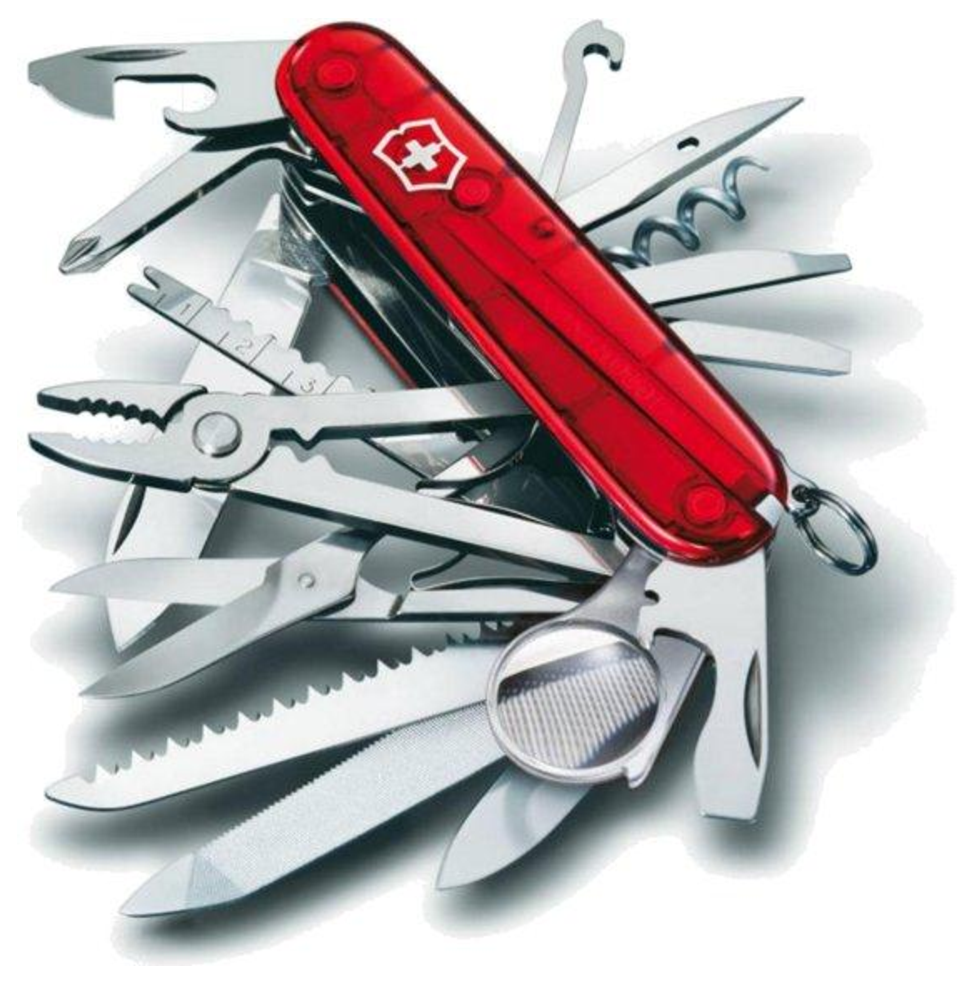
\includegraphics[height=100mm]{couteau-suisse}}
   \author{Vincent \textsc{Manet}}%\\[+2mm]
%   \textcolorgreen{\emph{manet.vim2\symbol{64}laposte.net}}}
   \maketitle
\else
   \thispagestyle{empty}\mbox{}%
   \AddToShipoutPicture*{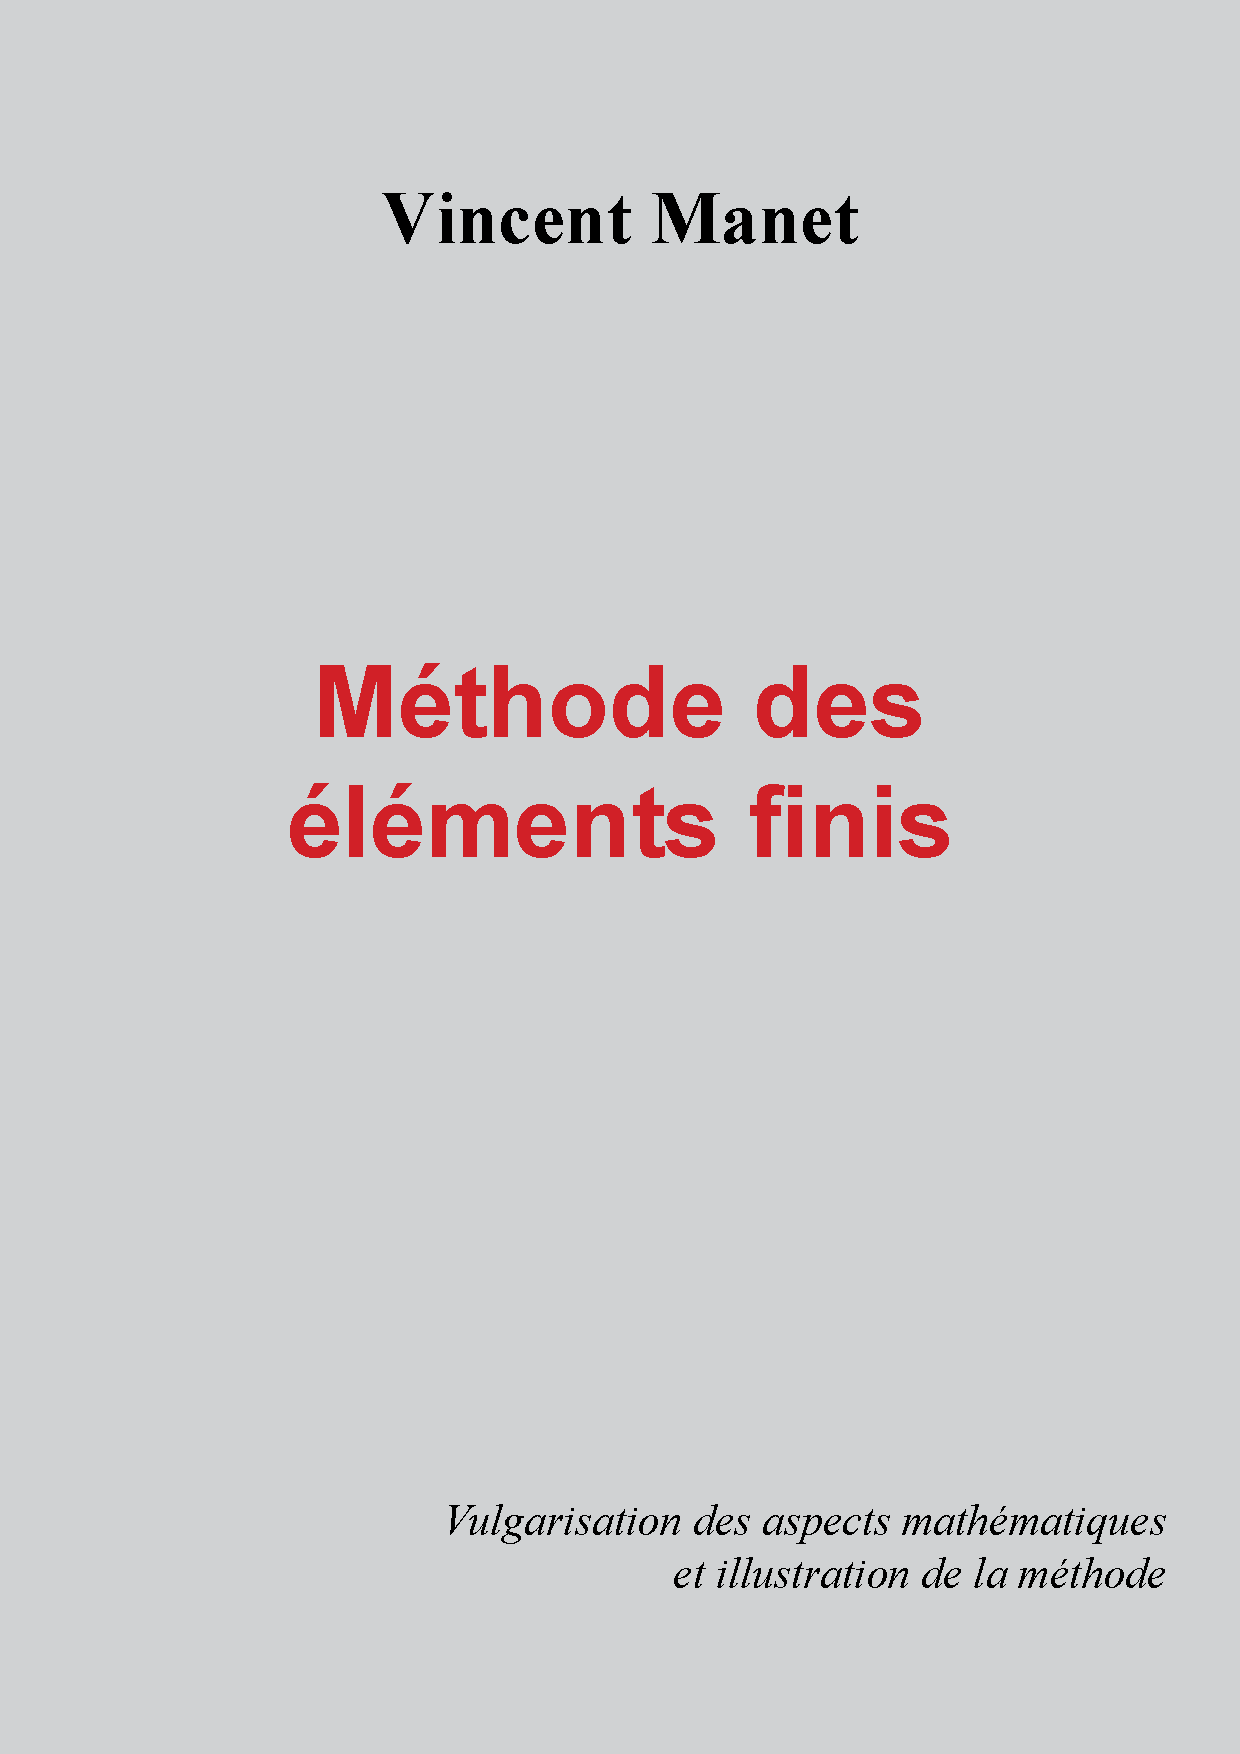
\includegraphics{Front}}%
%
   \setlength{\abovedisplayskip}{6pt plus 2pt minus 1pt}
   \setlength{\belowdisplayskip}{\abovedisplayskip}
   \setlength{\abovecaptionskip}{3pt}
   \setlength{\belowcaptionskip}{0pt}
   \title
\fi
% Verso de la page de titre
\newpage\mbox{}\thispagestyle{empty}%
\vspace*{2cm}

\vfill\normalsize\selectfont
\ifVersionDuDocEstVincent Ceci est la version<<~cours~>>{} de ce document.
\else
\noindent Vincent Manet --- 2013 (Ceci est la version <<~livre~>> {} de ce document)\\
Ce document est sous licence Creative Commons 3.0 France:
\begin{itemize}
\item paternité;
\item pas d'utilisation commerciale;
\item partage des conditions initiales à l'identique;
\end{itemize}
\url{http://creativecommons.org/licenses/by-nc-sa/3.0/deed.fr}\\[8pt]

\includegraphics[width=5cm]{IconTog.eps}
\fi
\newpage%  



\chapter*{Introduction}
%\addcontentsline{toc}{chapter}{Introduction}
\markboth{Introduction}{}

Dans ce (de moins en moins court) document, plutôt à destination d'ingénieurs
mécaniciens  connaissant déjà la méthode des éléments finis,
nous allons essayer de faire une présentation un peu plus théorique que ce qui 
leur est généralement proposé (et qui est quand même souvent de type 
<<~preuve par les mains~>>, ce qui occulte trop de points).

Nous ne ferons appel qu'à des notions mathématiques de bases généralement 
déjà vues pour la plupart en taupe (ou en tout début de cycle d'ingé)... bien
que des compléments que l'on peut qualifier d'élémentaires nous aient été
demandés et aient été inclus.

Nous espérons, grâce à cette présentation théorique
montrer toute la souplesse et la puissance de la méthode, afin
de permettre au lecteur d'envisager d'autres simulations que celles
qu'il a pu déjà réaliser par le passé.





\bigskip
\section*{But du document}
\markboth{But du document}{}
\addcontentsline{toc}{section}{But du document}

Le but initial était de \emph{présenter brièvement la théorie mathématique} derrière
les éléments finis afin que les ingénieurs utilisant cette méthode puisse en envisager
toutes les applications, ainsi que de \emph{couvrir les aspects qui}, selon nous, \emph{devraient être
connus de tout ingénieur mécanicien impliqué ou intéressé par le calcul numérique}.

Toutefois, il s'envisage comme \textcolorblue{support de référence à plusieurs cours}, 
cours qui ne portent pas sur tous les aspects traités dans ce document, et pendant lesquels les aspects 
pratiques sont plus développés (avec mise en situation sur machine).

\medskip
Même si nous avons voulu rester le plus succinct possible, l'introduction de
notions de proche en proche à conduit à un document fait aujourd'hui une
certaine taille (par exemple, nous avons besoins des espaces de Sobolev, mais
comment les introduire sans parler des espaces de Lebesgue, mais comment
les introduire sans parler...).

Aussi le document a-t-il finalement été découpé en plusieurs parties:
un survol des notions mathématiques, puis le traitement du problème
continu constituent l'ossature théorique nécessaire à assoir la MEF
sur un socle solide. La discrétisation par éléments finis à proprement parler
n'est aborder qu'ensuite, et d'ailleurs un seul chapitre suffirait à en faire
le tour... sauf à entrer plus dans le détail concernant <<~ce qui fâche~>>:
homogénéisation, non linéarité, dynamique, ce qui est fait dans des
chapitres séparés.

\medskip
Enfin, d'autres méthodes sont abordées car également très
employées aujourd'hui. Aussi est-il indispensable selon nous d'en avoir 
entendu parlé et d'en connaître les principales notions (BEM, FEEC...).

\medskip
En annexes, se trouve un petit fourre-tout comprenant des choses censées être 
maîtrisées depuis la taupe (mais qui parfois nous sont demandées) et les
compléments qui alourdiraient encore les propos précédents.

\medskip
Certaines notions (essentiellement de topologie) ne sont pas présentées dans ce 
document.
Il nous a semblé que le lecteur devait avoir quelques souvenirs de ce qu'est un
ouvert, un fermé, l'adhérence, la densité...
Par ailleurs, leur nom peut être suffisamment évocateur pour se passer d'une
définition formelle dans le contexte de ce document.

\bigskip
Attention, \textcolorred{ce document n'est pas un document de mathématiques}, il ne contient
d'ailleurs aucune preuve.
C'est, dans ces deux premières parties, un \textcolorblue{document de vulgarisation} de 
notions mathématiques nécessaires à une bonne compréhension de la méthode des éléments finis.

%\medskip
Nous avons voulu réaliser un survol des notions importantes, mais malgré tout, afin de ne
pas être parfois trop laconique, nous avons un peu débordé. \ifVersionDuDocEstVincent\textcolorgris{Dans ce cas, 
les passages considérés comme moins importants ont été mis en gris.}\fi

\medskip
\ifVersionDuDocEstVincent
D'ailleurs un certain <<~code couleur~>> sera plus ou moins respecté dans ce document.
En \textcolorblue{bleu} ou en \textcolorred{rouge}, les termes ou points importants,
en \textcolorgris{gris, les choses moins importantes} dont la lecture peut être
oubliée et enfin en
\textcolorgreen{vert, des remarques <<~de bon sens~>>} sur ce qui est exposé.
%\else
\fi

\medskip
En fin de document, un petit index des noms propres permettra au lecteur
de replacer les divers développements mentionnés dans l'histoire...
Il se peut qu'il subsistent quelques erreurs, notamment au niveau des
nationalités mentionnées, car il n'est pas toujours aisé de déterminer rapidement cette 
information (et nous ne connaissons pas toutes les biographies des personnes citées).

\medskip
\emph{Ce document a été réalisé très rapidement, et de manière extrêmement hachée.
Il comporte forcément encore beaucoup de fautes: merci de m'en faire part.}




\bigskip
\section*{Démarche de l'ingénieur numéricien}
\markboth{Preface}{Démarche de l'ingénieur numéricien}
\addcontentsline{toc}{section}{Démarche de l'ingénieur numéricien}

En préambule à ce document, nous tenions à synthétiser \textcolorblue{la
démarche complète de l'ingénieur numéricien}:
\begin{itemize}
   \item Modélisation / mise en équations -- Construction du problème continu (système d'EDP).
   \item Analyse mathématique du problème posé -- Existence, unicité, propriétés des solutions.
   \item Conception d'une méthode numérique -- Construction d'un problème discrétisé.
   \item Analyse numérique -- Questions de stabilité, convergence, précision.
   \item Algorithmique -- Choix de méthodes de résolution en dimension finie.
   \item Mise en œuvre sur ordinateur -- Programmation.
   \item Pre et Post Traitement (maillages / visualisation) -- Interpolation, extrapolation, outils de la CAO.
\end{itemize}

\medskip
Tous ces points ne seront évidemment pas abordés dans ce document!
\vfill
\noindent
\textcolorred{\textbf{Remerciements:}}

Nous n'avions pas prévu de réaliser une deuxième version aussi rapidement.
Celle-ci existe suite aux sollicitations de Mathias Legrand\index[aut]{Legrand (Mathias), ?- , Français}.
C'est lui  qui a développé les macros nécessaires à l'amélioration très très nette de la 
qualité typographique (environnements pour les notes historiques, les théorèmes, lemmes...).

C'est également pourquoi coexistent aujourd'hui deux versions (mais issues du même code source):
l'une que nous appelons <<~version cours~>> (plus en accord avec ce que nous proposons en cours),
et l'autre <<~version livre~>>, plus proche d'un ouvrage.

%\vfill
%
%\bigskip\colorgris
%\section*{Dans la même collection}
%
%Sont (ou seront) également disponibles les cours suivants:
%\begin{itemize}
%   \item calcul en fatigue des matériaux composites;
%   \item composites: lois de comportements, rupture, essais (et dynamique)
%   \item les structures algébriques;
%   \item l'acoustique numérique;
%   \item la mécanique stochastique;
%   \item le traitement du signal;
%   \item ...
%\end{itemize}


%\colorblack
%\medskip
%\colorgris
\tableofcontents%\markboth{Table des matières}{}
%\colorblack


%\bigskip
%\bibliographystyle{frunsrt}
%\bibliography{VM_MEF}
%\nocite{*}


% RIFF
% Lattice-Boltzmann

% \part{Survol mathématique}
% \chapter{Les espaces de base}\label{Ch-Esp}
\begin{abstract}
Dans les problèmes que nous envisageons de traiter \emph{in fine}, il n'est finalement
besoin que d'espaces vectoriels normés finis sur le corps des réels.
On pourrait rapidement en donner les principales propriétés qui sont sans doute encore
en mémoire des lecteurs tant elles sont «naturelles».

Mais en faisant cela, nous ne respecterions pas nos engagements de présenter un
peu plus avant les fondements mathématiques.

Sans toutefois aller trop loin dans les notions topologiques générales, nous allons
essayer dans ce chapitre de passer en revue la liste des espaces depuis les espaces
topologiques jusqu'aux espaces de Hilbert, de manière succincte et didactique (nous
l'espérons) en relevant les points importants essentiellement du point de vue de leur
utilité.
\end{abstract}

\section{Panorama non exhaustif des espaces}

\begin{histoire}%
Le mot «topologie» vient de la contraction des noms grecs «topos» (lieu) et «logos» (étude), c'est donc l'étude du lieu. On a d'ailleurs commencé par l'appeler \emph{Analysis Situs}, le terme «topologie» n'étant introduit qu'en 1847, en allemand, par Johann Benedict Listing dans Vorstudien zur Topologie.\index[aut]{Listing (Johann Benedict), 1808-1882, Allemand}

La topologie vise à définir ce qu'est un lieu (i.e. un espace) et quelles peuvent être ses propriétés (je dirais uniquement en tant que tel, sans autre ajout). Elle s'intéresse plus précisément à ce que l'on appelle aujourd'hui espaces topologiques et aux applications, dites continues, qui les lient, ainsi qu'à leurs déformations (``\emph{A topologist is one who doesn't know the difference between a doughnut and a coffee cup}'').

\sbox{\MaBoiteAvecPhotos}{\setlength{\tabcolsep}{0pt}\scriptsize%
\begin{tabular}{ccc}%
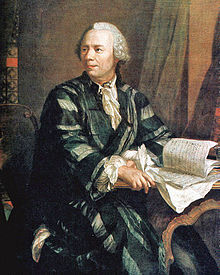
\includegraphics[height=\the\HauteurDesPhotos]{Euler}&%
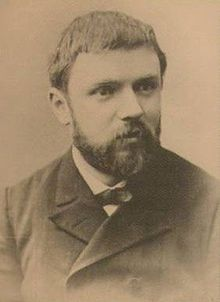
\includegraphics[height=\the\HauteurDesPhotos]{Poincare}&%
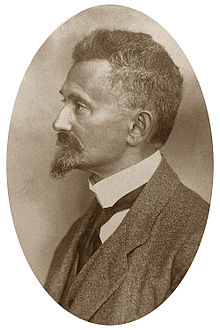
\includegraphics[height=\the\HauteurDesPhotos]{Hausdorff}\\%
Euler&Poincaré&Hausdorff%
\end{tabular}}
\medskip
\ImageADroite{%
En analyse, elle fournit des informations sur l'espace considéré permettant d'obtenir un certain nombre de résultats (existence et/ou unicité de solutions d'équations au dérivées partielles, notamment). Les espaces métriques ainsi que les espaces vectoriels normés sont des exemples d'espaces topologiques. L'origine de la topologie est l'étude de la géométrie dans les cultures antiques. Le travail de Leonhard Euler\index[aut]{Euler (Leonhard Paul), 1707-1783, Suisse} datant de 1736 sur le problème des sept ponts de Königsberg est considéré comme l'un des premiers résultats de géométrie qui ne dépend d'aucune mesure, i.e. l'un des premiers résultats topologiques.
}

Henri Poincaré\index[aut]{Poincaré (Henri), 1854-1912, Français} publia \emph{Analysis Situs} en 1895, introduisant les concepts d'homotopie et d'homologie. Bien d'autres mathématiciens ont contribué au sujet parmi lesquels nous citerons: Cantor, Volterra, Arzelà, Hadamard, Ascoli, Fréchet, Hausdorff...\index[aut]{Cantor (Georg Ferdinand Ludwig Philip), 1845-1918, Allemand}\index[aut]{Hadamard (Jacques Salomon), 1865-1963, Français}\index[aut]{Ascoli (Giulio), 1843-1896, Italien}\index[aut]{Fréchet (Maurice René), 1878-1973, Français}\index[aut]{Hausdorff (Felix), 1868-1942, Allemand}

Finalement, une dernière généralisation en 1922, par Kuratowski, donna le concept actuel d'espace topologique.\index[aut]{Kuratowski (Kazimierz), 1896-1980, Polonais}
\end{histoire}
\colorblack


\newpage
\subsection{Point de vue topologique}

\medskip
\begin{marge}
\noindent\tikz[remember picture,baseline] \node[fill=ocre!10,inner sep=3pt](t1) {$E$, un ensemble};

{\small \colorgreen
\noindent
Cela suffit déjà pour pouvoir s'intéresser par exemple à des fonctions, à des relations d'équivalence (donc au quotient)... décomposition canonique, permutation...

On peut ensuite définir un ensemble ordonné...}

\medskip %\noindent
\textcolorblue{Une topologie}\index{topologie}~$T$ est
un ensemble de parties de~$E$ que l'on définit comme les ouverts de~$(E,T)$, vérifiant les propriétés suivantes:
\begin{itemize}
  \item L'ensemble vide et~$E$ appartiennent à~$T$.
  \item Toute réunion quelconque d'ouverts est un ouvert, i.e. si~$(O_i)_{i\in I}$ est une famille 	d'éléments de~$T$, indexée par un ensemble~$I$ quelconque (pas nécessairement fini ni 	même dénombrable) alors~$\bigcup_{i \in I}O_i \in T$.
  \item Toute intersection finie d'ouverts est un ouvert, i.e. si~$O_1, ..., O_n$ sont des éléments de~$T$ (avec~$n > 0$), alors~$O_1\cap \ldots \cap O_n \in T$.
\end{itemize}

\medskip
\noindent\tikz[remember picture,baseline] \node[fill=ocre!10,inner sep=3pt](t2) {Espace topologique};\index{espace!topologique}

{\small \colorgreen\noindent
À partir des ouverts, on définit les fermés, l'adhérence, l'intérieur, l'extérieur, voisinage...}

\medskip
\textcolorblue{Séparation}: % (dit aussi «axiome~$T_2$» au sein des axiomes de séparation):

deux points distincts quelconques admettent toujours des voisinages disjoints.

\medskip
\noindent\tikz[remember picture,baseline] \node[fill=ocre!10,inner sep=3pt](t3) {Espace séparé (ou de Hausdorff)};\index{espace!séparé}\index{espace!de Hausdorff}\index[aut]{Hausdorff (Felix), 1868-1942, Allemand}

{\small \colorgreen
\noindent Intérêts:
\begin{itemize}
  \item Unicité de la limite de tout filtre convergent.
  \item Une suite convergente a une limite unique.
  \item Une topologie plus fine qu'une topologie séparée est séparée.
  \item Tout sous-espace d'un espace séparé est séparé.
  \item Deux applications continues à valeurs dans un séparé qui coïncident sur une partie dense sont égales.
\end{itemize}
}

\medskip
\textcolorblue{Régularité}:

Il est possible de séparer un point~$x$ et un fermé~$F$ ne contenant pas~$x$ par deux ouverts disjoints.

On peut même alors choisir ces deux ouverts de manière à ce que leurs adhérences respectives soient disjointes.

\medskip
\noindent\tikz[remember picture,baseline] \node[fill=ocre!10,inner sep=3pt] (t4) {Espace régulier};\index{espace!régulier}

{\small \colorgreen
\noindent Application:
\begin{itemize}
  \item Tout point admet une base de voisinages fermés.
  \item Tout fermé est l'intersection de ses voisinages fermés.
\end{itemize}
}

\medskip
\textcolorblue{Compacité} (recouvrement fini):\index{compacité}

Un espace séparé est compact (vérifie la propriété de Borel-Lebesgue), si chaque fois qu'il est recouvert par des ouverts, il est recouvert par un nombre fini d'entre eux.

\medskip
\noindent\tikz[remember picture,baseline] \node[fill=ocre!10,inner sep=3pt] (t5) {Espace compact};\index{espace!compact}

{\small \colorgreen \noindent L'intérêt des compacts est de pouvoir étendre des propriétés trivialement vérifiées par des applications définies sur un ensemble fini à des applications définies sur des espaces topologiques infinis, à condition bien sûr qu'elles soient continues.

\noindent Tout produit de compacts est compact.

\noindent $\overline{\RR}$ est compact

\noindent Un espace peut ne pas être compact, mais une de ses parties l'être:
\begin{itemize}
  \item~$\RR$ n'est pas fermé, mais tout~$[a;b]$ fermé borné l'est.
  \item~$\RR^n$ n'est pas compact, mais tout pavé fermé l'est (voir théorème \ref{Th-BL}).
\end{itemize}
}
\begin{tikzpicture}[remember picture,overlay]
  \draw[->,thick,ocre] (t1.west) -- +(-10pt,0) |-([yshift=2pt]t2.west);
  \draw[->,thick,ocre] ([yshift=-2pt]t2.west) -- +(-10pt,0) |-([yshift=2pt]t3.west);
  \draw[->,thick,ocre] ([yshift=-2pt]t3.west) -- +(-10pt,0) |-([yshift=2pt]t4.west);
  \draw[->,thick,ocre] ([yshift=-2pt]t4.west) -- +(-10pt,0) |-(t5.west);
\end{tikzpicture}
\end{marge}

\medskip
\textcolorred{Notons bien que rien n'est dit sur les éléments de l'ensemble~$E$. Ce peuvent être des éléments discrets, des scalaires, des vecteurs, des fonctions...}

\newpage
\subsection{Point de vue métrique}
Comme nous le mentionnions au paragraphe précédent, lorsque l'on parle d'espace
on a intuitivement envie de parler de «distance».

%\medskip
\begin{histoire}
Unifiant les travaux de ses prédécesseurs sur les espaces de fonctions, c'est en 1906 que Maurice Fréchet introduit le concept d'espace métrique.\index[aut]{Fréchet (Maurice René), 1878-1973, Français}

\sbox{\MaBoiteAvecPhotos}{\setlength{\tabcolsep}{0pt}\scriptsize%
\begin{tabular}{cc}%
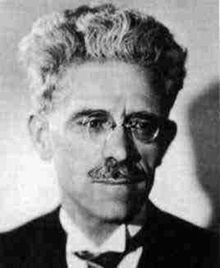
\includegraphics[height=\the\HauteurDesPhotos]{Frechet}&%
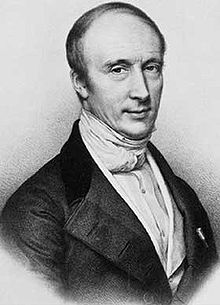
\includegraphics[height=\the\HauteurDesPhotos]{Cauchy}\\%
Fréchet&Cauchy%
\end{tabular}}
\medskip
\ImageADroite{%
La métrique qui nous est la plus usuelle est évidemment la métrique euclidienne,\index[aut]{Euclide, -325-- -265, Grec} qui est celle que nous utilisons en géométrique «classique» (euclidienne): la distance entre deux points est égale à la longueur du segment les reliant.
La structure métrique fournit beaucoup plus d'information sur la forme géométrique des objets que la structure topologique.\\
\indent
Enfin nous redonnerons le si important critère de Cauchy\index[aut]{Cauchy (Augustin Louis, baron -), 1789-1857, Français} (qui est valable pour tout espace uniforme, dont notamment les espaces métriques) qui permet de définir la toute aussi importante notion de complétude.}
\end{histoire}
\colorblack

\medskip
\begin{marge}%
\noindent\tikz[remember picture,baseline] \node[fill=ocre!10,inner sep=3pt] (n1) {$E$, un ensemble};

Une \textcolorblue{distance ou métrique}~$d$\index{distance}\index{métrique}
est une application de~$E\times E \rightarrow \RR_+$ telle que:
\begin{itemize}
  \item~$d(x,y)=d(y,x)$ (symétrie);
  \item~$d(x,y)>0$ si~$x\ne y$, et~$d(x,x)=0$ (positivité);
  \item~$d(x,z)\le d(x,y)+d(y,z)$ (inégalité triangulaire).
\end{itemize}

\medskip
\noindent\tikz[remember picture,baseline] \node[fill=ocre!10,inner sep=3pt] (n2) {Espace métrique\index{espace!métrique}};

{\small \colorgreen\noindent
On peut réexprimer les notions d'ouvert, fermé, adhérence... densité, continuité... avec la métrique
(les~$\varepsilon$...).

\noindent Deux normes sont équivalentes si elles définissent la même topologie.

\noindent Deux normes~$\|\cdot\|_1$ et~$\|\cdot\|_2$ sont équivalentes s'il existe deux constantes strictement positives~$k'$ et~$k''$ telles que $\forall x\in E$, $\|x\|_1\le k'\|x\|_1$ et $\|x\|_2\le k'' \|x\|_1$.}

\medskip
\textcolorblue{Critère de Cauchy:}\index{critère de Cauchy}\index[aut]{Cauchy (Augustin Louis, baron -), 1789-1857, Français}

Soit~$E$ un espace métrique et soit~$x_0$, $x_1$, ..., $x_n$, ...
une suite d'éléments de~$E$.
Cette suite est de Cauchy de~$E$ si:
\begin{equation}
\forall\varepsilon>0, \exists N\in\NN, (\forall n\in\NN, \forall m\in\NN,
n\ge N, m\ge N): d(x_m,x_n)\le\varepsilon
\end{equation}
ou encore:~$d(x_m,x_n)$ tend vers~$0$ quand~$m$ et~$n$ tendent
vers l'infini.

\medskip
\noindent \tikz[remember picture,baseline] \node[fill=ocre!10,inner sep=3pt] (n3) {Espace métrique complet\index{espace!métrique!complet}};

{\small \colorgreen\noindent
Toute suite convergente est de Cauchy.

\noindent Réciproque: si~$x_0$, $x_1$, ..., $x_n$, ... est de Cauchy sur
$\RR$ ou~$\CC$, alors elle converge.
}

\medskip\noindent
\textcolorred{Cette propriété est fondamentale car elle permet de reconnaître si une suite
converge sans connaître sa limite.}
%Mais attention, ce n'est pas vrai quelque soit l'espace métrique, mais sur~$\RR$ et~$\CC$.

\medskip\noindent
Attention, la notion d'espace complet est une notion métrique et non topologique
(elle peut donc être vraie pour une métrique et fausse pour une autre).

\medskip\noindent
\textcolorred{L'importance de la complétude} tient à ce que la solution d'un problème passe souvent
par une solution approchée. Si la suite des solutions approchées est de Cauchy d'un espace convenable,
et si cet espace est complet, alors la convergence vers une solution du problème est assurée.
\begin{tikzpicture}[remember picture,overlay]
  \draw[->,thick,ocre] (n1.west) -- +(-10pt,0) |-([yshift=2pt]n2.west);
  \draw[->,thick,ocre] ([yshift=-2pt]n2.west) -- +(-10pt,0) |-(n3.west);
\end{tikzpicture}
\end{marge}

\medskip
\subsection{Point de vue algébrique}

\medskip
Jusqu'à présent, nous n'avons pas vraiment parlé d'opérations que nous pourrions effectuer à l'intérieur des espaces que nous avons définis, ou entre ces espaces.
\textcolorgris{\small Pour une présentation des structures algébriques on se reportera au cours homonyme. Elles sont riches et nombreuses. Dans le cadre de ce document, nous ne nous intéresserons qu'au cas de la structure d'espace vectoriel, le but étant, comme mentionné en introduction, d'en arriver aux espaces de Hilbert, fondements de l'analyse fonctionnelle.}

\medskip
\begin{histoire}
Lorsque l'on demande de citer l'un des grands mathématiciens du \textsc{xx}\fup{e} siècle, Henri Poincaré\index[aut]{Poincaré (Henri), 1854-1912, Français} et David Hilbert\index[aut]{Hilbert (David), 1862-1943, Allemand} se partagent souvent la première place, aussi bien pour l'éventail considérable des sujets qu'ils ont abordés que pour avoir fait émerger de nombreuses idées fondamentales.

\sbox{\MaBoiteAvecPhotos}{\setlength{\tabcolsep}{0pt}\scriptsize%
\begin{tabular}{cc}%
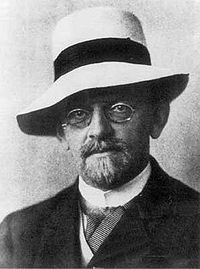
\includegraphics[height=\the\HauteurDesPhotos]{Hilbert}&%
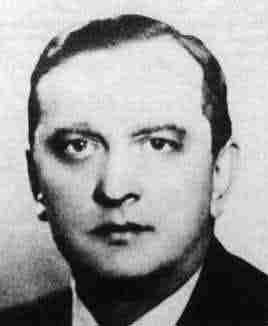
\includegraphics[height=\the\HauteurDesPhotos]{Banach}\\%
Hilbert&Banach%
\end{tabular}}
\medskip
\ImageADroite{%
Hilbert reste célèbre pour ses 23 problèmes (dits problèmes de Hilbert) qu'il présenta au deuxième congrès international des mathématiciens à Paris en 1900, qui tenaient jusqu'alors les mathématiciens en échec et devaient marquer le cours des mathématiques du \textsc{xx}\fup{e} siècle (et il avait raison; tous ne sont pas résolus à ce jour).
Notons que c'est von Neumann,\index[aut]{Neumann (John, von -), 1903-1957, Hongrois} reprenant les travaux de Hilbert, qui formalise et nomme ces espaces les espaces de Hilbert en 1927.\\
\indent
Nous croiserons également un autre fondateur de l'analyse fonctionnelle, Stephan Banach\index[aut]{Banach (Stephan), 1892-1945, Polonais} qui a généralisé entre autre les travaux de Hilbert sur les équations intégrales, notamment en approfondissant la théorie des espaces vectoriels topologiques.}
\end{histoire}
\colorblack


\medskip
\begin{marge}
\noindent\tikz[remember picture,baseline] \node[fill=ocre!10,inner sep=3pt] (b1) {$E$, un ensemble};

\medskip
\textcolorblue{Structure d'espace vectoriel}:

C'est une structure comportant une loi de composition interne et une loi de composition externe sur un corps~$\KK$ permettant d'effectuer des combinaisons linéaires (voir cours sur les structures algébriques).

La loi de composition interne, notée~$+$ en fait un groupe abélien, la loi de composition externe est la multiplication par un scalaire, scalaire pris sur le corps~$\KK$ considéré.

\medskip
\noindent\tikz[remember picture,baseline] \node[fill=ocre!10,inner sep=3pt] (b2) {Espace vectoriel (topologique)\index{espace!vectoriel!topologique}};

{\small \colorgreen\noindent Sur un espace vectoriel de dimension finie sur~$\RR$ ou~$\CC$, deux normes quelconques sont équivalentes.}

\medskip
Une \textcolorblue{norme sur un espace vectoriel}~$E$\index{norme} est une fonction, $x \mapsto \|x\|$ possédant les propriétés:
\begin{itemize}
  \item positivité:~$\|x\|>0$ pour~$x\ne0$, $\|0\|=0$;
  \item transformation par les homothéties:~$\|\lambda x\|=|\lambda|\| x\|, \lambda\in\KK$;
  \item inégalité de convexité:~$\|x+y\|\le\|x\|+\|y\|$.
\end{itemize}

La \textcolorblue{distance issue de la norme} est la distance définie par~$d(x,y)=\|x-y\|$.

\medskip
\noindent\tikz[remember picture,baseline] \node[fill=ocre!10,inner sep=3pt] (b3) {Espace vectoriel normé\index{espace!vectoriel!normé}};

{\small \colorgreen\noindent Tout espace vectoriel normé est automatiquement un espace métrique (avec la distance issue de sa norme).\index{distance!issue d'une norme} De plus:
\begin{itemize}
  \item la distance est invariante par translation:~$d(x-a,y-a)=d(x,y)$.
  \item une homothétie de rapport~$\lambda$ multiplie la distance par~$|\lambda|$:~$d(\lambda x,\lambda y)=|\lambda| d(x,y)$.
\end{itemize}

\noindent Tout espace vectoriel normé de dimension finie est localement compact (i.e. tout point possède au moins un voisinage compact), car toute boule fermée est compacte.

\noindent L'intérêt des distances issues d'une norme est qu'elles rendent continues les opérations de l'espace vectoriel et qu'en particulier les translations sont des homéomorphismes.
}

\medskip
Comme un espace vectoriel normé muni avec la distance issue de sa norme est un espace métrique, on peut se demander si cet espace métrique vérifie le \textcolorblue{critère de Cauchy} (voir paragraphe précédent) afin d'en faire un espace complet.

\medskip
\noindent\tikz[remember picture,baseline] \node[fill=ocre!10,inner sep=3pt](b4) {Espace de Banach\index{espace!de Banach}\index[aut]{Banach (Stephan), 1892-1945, Polonais}};
\begin{tikzpicture}[remember picture,overlay]
  \draw[->,thick,ocre] (b1.west) -- +(-10pt,0) |-([yshift=2pt]b2.west);
  \draw[->,thick,ocre] ([yshift=-2pt]b2.west) -- +(-10pt,0) |-([yshift=2pt]b3.west);
  \draw[->,thick,ocre] ([yshift=-2pt]b3.west) -- +(-10pt,0) |-([yshift=2pt]b4.west);
\end{tikzpicture}

{\small \colorgreen\noindent
C'est donc finalement un espace vectoriel normé sur un sous-corps $\KK$ de~$\CC$ (en général, $\KK=\RR$ ou~$\CC$), complet pour la distance issue de sa norme.

\noindent Comme la topologie induite par sa distance est compatible avec sa structure d'espace vectoriel, c'est un espace vectoriel topologique.
}

\medskip
Une norme~$\|\cdot\|$ \textcolorblue{découle d'un produit scalaire ou hermitien}\index[aut]{Hermite (Charles), 1822-1901, Français}\index{produit scalaire} $\langle\cdot,\cdot\rangle$ si l'on a:~$\| x\| = \sqrt{\langle x,x \rangle}$.

\medskip
\noindent\tikz[remember picture,baseline] \node[fill=ocre!10,inner sep=3pt](b5) {Espace de Hilbert\index{espace!de Hilbert}\index[aut]{Hilbert (David), 1862-1943, Allemand}};
\begin{tikzpicture}[remember picture,overlay]
  \draw[->,thick,ocre] ([yshift=-2pt]b4.west) -- +(-10pt,0) |-(b5.west);
\end{tikzpicture}

{\small \colorgreen\noindent C'est donc un espace préhilbertien complet, i.e. un espace de Banach dont la norme découle d'un produit scalaire ou hermitien\index[aut]{Hermite (Charles), 1822-1901, Français} \textcolorred{unique}.

\noindent Un espace de Hilbert est la généralisation en dimension quelconque d'un espace euclidien\index[aut]{Euclide, -325-- -265, Grec} ou hermitien\index[aut]{Hermite (Charles), 1822-1901, Français} (Un \textbf{espace vectoriel euclidien} est un espace vectoriel réel de dimension finie muni d'un produit scalaire).
}
\end{marge}

\medskip
\textcolorred{Le plus important} est de disposer d'un produit scalaire, car on va alors pouvoir déterminer des parties orthogonales de l'espace, donc en somme directe (voir théorème~\ref{th:projHilbert}).

	On rappelle, si besoin, qu'un \textcolorblue{produit scalaire}\index{produit scalaire} est une forme bilinéaire\index{forme!bilinéaire} (i.e. une application\index{application} de~$E\times E$ dans~$\RR$, linéaire pour chacune des deux variables) possédant les propriétés:
	\begin{itemize}
	  \item symétrie:~$\forall x,y \in E$, $\langle x\, , \, y \rangle = \langle y\, , \, x\rangle$
	  \item positivité:~$\forall x \in E$, $\langle x\, , \, x \rangle \; \ge \; 0$
	  \item définie:~$\forall x \in E$, $\big(\ \langle x\, , \, x \rangle = 0 \; \Rightarrow x = 0\ \big)$
	\end{itemize}
ce qui se traduit pas la définition: «Un produit scalaire sur un espace vectoriel réel~$E$ est une forme bilinéaire symétrique définie positive».

\medskip
%On dispose également du théorème suivant, particulièrement utile.
\begin{theoreme}\label{Th-SsH}
Tout sous-espace vectoriel fermé d'un espace de Hilbert est un espace de Hilbert.
\end{theoreme}

\medskip
Voici quelques espaces de Banach couramment utilisés:
\begin{itemize}
\item Les espaces euclidiens\index[aut]{Euclide, -325-- -265, Grec}~$\RR^n$ et
les espaces hermitiens\index[aut]{Hermite (Charles), 1822-1901, Français}~$\CC^n$
munis de la norme:
\begin{equation}\|(x_1,\ldots,x_n)\| = \sqrt{\dsum_{i=1}^n x_i \overline{x_i}}\end{equation} où~$\overline{x_i}$
désigne le conjugué de~$x_i$.

\item L'espace des fonctions (dans~$\RR$ ou~$\CC$) continues et bornées sur un espace topologique~$X$,
muni de la norme~$\|f\| = \sup_{x \in X}(|f(x)|)$.
En particulier, l'espace des fonctions continues sur un espace~$X$ compact, comme un intervalle réel~$\intff{a}{b}$.

\item Pour tout réel~$p \ge 1$, l'espace~$L^p$ des classes de fonctions mesurables, dans~$\RR$ ou~$\CC$, sur un espace mesuré~$X$.
\end{itemize}

\medskip
Voici quelques espaces de Hilbert classiques:
\begin{itemize}
  \item L'espace euclidien\index[aut]{Euclide, -325-- -265, Grec}~$\RR^n$ muni du produit scalaire usuel est hilbertien,\index[aut]{Hilbert (David), 1862-1943, Allemand} 
  \item L'espace~$L^2$ des fonctions de carré intégrable (voir chapitre~\ref{Ch-Lp}).
  \item Certains espaces de Sobolev (voir chapitre~\ref{Ch-Sobo}) sont des espaces de Hilbert (ceux qui nous intéresserons en général, ça tombe bien).
\end{itemize}

\medskip
\begin{theoreme}[Théorème de complétion sur un espace de Banach]\label{th:complbanach}\index{théorème!de complétion (sur un Banach)}
Soit~$E$ un espace vectoriel normé incomplet.
Alors~$E$ est isomorphe, en tant qu'espace vectoriel, et isométrique à un sous-espace vectoriel dense dans un espace de Banach~$\overline{E}$.

Cet espace de Banach~$\overline{E}$ est unique à un isomorphisme isométrique près.
\end{theoreme}

Ce théorème de complétion répond par l'affirmative à la question: si l'espace normé~$E$ n'est pas complet, existe-t-il un Banach minimal~$\overline{E}$ le
contenant ?

\medskip
\begin{theoreme}[Théorème de projection dans un espace de Hilbert]\label{th:projHilbert}\index{théorème!de projection (dans un Hilbert)}
Soit~$F$ un sous-espace vectoriel fermé d'un espace de Hilbert~$H$ (il est alors lui-même un espace de Hilbert d'après le théorème~\ref{Th-SsH}). Alors:
\begin{itemize}
  \item son orthogonal~$F^\bot$, qui est l'ensemble des vecteurs orthogonaux à chaque 	vecteur de~$F$, est un sous-espace vectoriel fermé (donc est aussi un espace de Hilbert, toujours en vertu du théorème~\ref{Th-SsH});
  \item et est également le supplémentaire de $F$: tout~$h\in H$ s'écrit de façon unique~$h=h'+h''$ où~$h'$ est le projeté orthogonal de~$h$ sur~$F$, et~$h''$ le projeté orthogonal de~$h$ sur~$F^\bot$.
\end{itemize}

\medskip
Ainsi, $F^\bot$ est l'orthogonal et le supplémentaire de $F$, et ces deux sous-espaces sont donc en sommes directe. On a donc=~$H=F\oplus F^\bot$ (on utilise parfois le terme de «somme hilbertienne»).
\end{theoreme}

\textcolorgris{Ce résultat subsiste si l'on suppose seulement que $H$ est un espace préhilbertien et que $F$ est un sous-espace vectoriel complet de $H$.}

\medskip\ifVersionDuDocEstVincent\else\newpage\fi
\section{Tribu, mesure, espaces mesurable et mesuré}\label{Sec-Mesure}

En complément à l'aspect métrique (Fréchet 1906),\index[aut]{Fréchet (Maurice René), 1878-1973, Français} nous allons maintenant aborder l'aspect mesure.

\medskip
\textcolorgreen{Le but, à travers la notion de mesure}, est d'étendre la notion usuelle de longueur pour les ensembles de~$\RR$, ou de volume pour ceux de~$\RR^n$, et ceci de deux manières:
\begin{itemize}
\item on veut d'une part pouvoir considérer des espaces de base plus généraux (plus «abstraits»: espaces de dimension infinie, espaces sur lesquels on définit les probabilités...); 
\item et d'autre part on veut englober dans le même cadre mathématique les notions de longueurs, surface, volume, mais aussi de masses ou charges ponctuelles issues de la mécanique, de l'électricité... car toutes ces quantités possèdent une même propriété évidente: l'\textcolorblue{additivité} (i.e. si l'on désigne par~$\mu(A)$ le volume, la masse, la charge électrique... d'une partie «raisonnable»~$A$, alors~$\mu(A\cap B)=\mu(A)+\mu(B)$ dès que~$A$ et~$B$ sont disjoints).
\end{itemize}

\medskip
Afin de réaliser cela, il faut en passer par quelques complications mathématiques, et cela essentiellement pour deux raisons:
\begin{itemize}
   \item Il nous faut tout d'abord définir ce qu'est une partie «raisonnable» d'un ensemble~$E$ (s'il est aisé de définir le volume d'un polyèdre par exemple, il existe des parties dont la «frontière» est si complexe qu'elles ne possèdent pas de notion de volume).

   \item Ensuite, la propriété d'additivité si dessus est un peu trop naïve et se révèle insuffisante pour avoir de bonnes propriétés pour les mesures.

En effet, la classe des mesures additives a une structure mathématique extrêmement pauvre, ne permettant pas, en particulier, de définir une notion satisfaisante d'intégrale par rapport à ces mesures additives.
On est donc conduit à utiliser les mesures possédant la propriété de~$\sigma$-additivité (voir définition d'une mesure ci-dessous), ce qui nous oblige à considérer comme classe d'ensembles «mesurables» une tribu (voir définition~\ref{Def-tribu}) au lieu de la notion plus simple d'algèbre.
\end{itemize}

\medskip
\begin{definition}[Algèbre]
Une \textcolorblue{algèbre (de Boole)\index[aut]{Boole (George), 1815-1864, Anglais}~$\mathcal{E}$} sur un ensemble $X$ est un \textcolorred{ensemble} non vide de parties de~$X$, stable par passage au complémentaire et par union finie (donc aussi par intersection finie), i.e.:
\begin{enumerate}
 \item~$\mathcal{E} \not=\varnothing$
 \item~$\forall A \in \mathcal{E}$, ${}^c A \in\mathcal{E}$, où~${}^cA$ désigne le complémentaire de~$A$ dans~$X$.
	(donc~$X\in \mathcal{A}$)
\item si~$A_1,\ldots,A_n$~$\in\mathcal{E}$ alors~$A_1\cup ...\cup A_n \in\mathcal{E}$
\end{enumerate}
\end{definition}

\medskip
\begin{definition}[Tribu]\label{Def-tribu}
Une \textcolorblue{tribu~$\mathcal{A}$}\index{tribu} sur un ensemble~$X$ est un \textcolorred{ensemble} non vide de parties de~$X$, stable par passage au complémentaire et par union dénombrable (donc aussi par intersection dénombrable), i.e.:
\begin{enumerate}
 \item~$\mathcal{A} \not=\varnothing$
 \item~$\forall A \in \mathcal{A}$, ${}^c A \in\mathcal{A}$%, où~${}^cA$ désigne le complémentaire de~$A$ dans~$X$. (donc~$X\in \mathcal{A}$)
\item si~$\forall n \in \mathbb{N}$, $A_n \in\mathcal{A}$ alors~$\bigcup_{n\in\mathbb{N}} A_n \in\mathcal{A}$
\end{enumerate}
\end{definition}
\medskipvm
Ces deux dernières définitions étant placées l'une sous l'autre, leur différence doit apparaître clairement: dans le cas d'une algèbre, on a à faire à un nombre fini d'intersection ou de réunions, dans celui d'une tribu, on prend en compte un ensemble dénombrable (donc fini ou non).

\medskip
Il est donc évident que toute tribu est une algèbre, la réciproque étant fausse.

\medskip
\begin{definition}[Espace mesurable]
Le couple \textcolorblue{$(X,\mathcal{A})$} est appelé \textcolorblue{espace mesurable}\index{espace!mesurable (probabilisable)} ou espace probabilisable en fonction du contexte.
Sur les espaces mesurables on définit des mesures (voir ci-après); sur les espaces probabilisables, on appelle ces mesures des probabilités.
\end{definition}

\medskip
\begin{histoire}
La théorie de la mesure s'occupe de regarder un peu plus en détail ce qui se passe à l'intérieur des espaces dits mesurés (définis plus bas): il s'agit de mesurer les différentes parties existant dans un tel espace, parties en lien avec la topologie, ce qui reboucle le sujet...

\medskip
Lorsque l'on évoque le concept de mesure, on en arrive assez rapidement à se demander: Est-ce que l'on peut tout mesurer? Est-ce que l'on doit tout mesurer? Qu'est-ce qui est négligeable ?

\sbox{\MaBoiteAvecPhotos}{\setlength{\tabcolsep}{0pt}\scriptsize%
\begin{tabular}{ccc}%
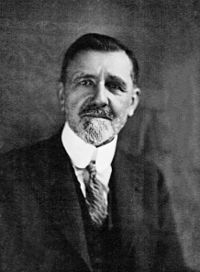
\includegraphics[height=\the\HauteurDesPhotos]{Borel}&%
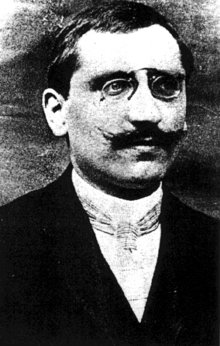
\includegraphics[height=\the\HauteurDesPhotos]{Lebesgue}&%
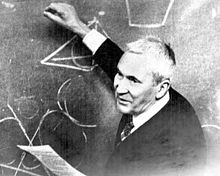
\includegraphics[height=\the\HauteurDesPhotos]{Kolmogorov}\\%
Borel &Lebesgue &Kolmogorov%
\end{tabular}}
\medskip
\ImageADroite{%
En 1894, Émile Borel\index[aut]{Borel (Félix Édouard Justin Émile), 1871-1956, Français} énonce la première définition d'ensemble négligeable.
En 1897, il définit les ensembles mesurables.
En 1901, Henri-Léon Lebesgue\index[aut]{Lebesgue (Henri-Léon), 1875-1941, Français}  introduit la notion de mesure.
La théorie se développe jusque dans les années 1950.\\\indent
Andreï Kolmogorov\index[aut]{Kolmogorov (Andreï Nikolaïevitch), 1903-1987, Russe} proposera une axiomatisation du calcul des probabilités basée notamment sur l'intégrale définie à partir d'une mesure.
}
\end{histoire}

\medskip
Les parties de~$X$ qui appartiennent à la tribu~$\mathcal{A}$ sont appelées \textcolorblue{ensembles mesurables}.\index{ensemble mesurable}
Dans un contexte probabiliste, on les appelle événements (il suffit que~$\mu(X)=1$ pour que~$\mu$ soit une probabilité).

%\medskip
Une \textcolorblue{mesure~$\mu$}\index{mesure} sur un ensemble~$X$ est une fonction qui associe à chaque élément d'une tribu d'un ensemble~$X$ un \textcolorred{scalaire positif} (une longueur, un volume, une probabilité...).

\begin{definition}[Mesure]
\medskip
Soit~$(X,\mathcal{A})$, un espace mesurable.
Une application~$\mu$ définie sur~$\mathcal{A}$, à valeurs dans~$[0,+\infty]$ est appelée
mesure lorsque les deux propriétés suivantes sont satisfaites:
\begin{enumerate}
  \item L'ensemble vide a une mesure nulle:~$\mu\left(\varnothing\right)=0$
  \item L'application~$\mu$ est~$\sigma$-additive:
si~$E_1$, $E_2$, ... est une famille dénombrable de parties de~$X$ appartenant à
$\mathcal{A}$ et si ces parties sont deux à deux disjointes, alors la mesure~$\mu(E)$ de leur réunion
$E$ est égale à la somme des mesures des parties:
\begin{equation}
\mu\left(\bigcup_{k=1}^{\infty}E_{k}\right)=\sum_{k=1}^{\infty}\mu(E_{k}).1
\end{equation}
\end{enumerate}
\end{definition}

On appelle \textcolorblue{espace mesuré un triplet~$(X,\mathcal{A},\mu)$},
\index{espace!mesuré} où~$X$ est un ensemble, $\mathcal{A}$ une tribu sur
$X$ et~$\mu$ une mesure sur~$\mathcal{A}$.

\medskip
\colorgris
Soient~$(X,T)$ et~$(Y,U)$ deux espaces mesurables.
On appelle rectangle mesurable du produit~$\Omega=X\times Y$, toute partie de~$\Omega$ de la forme~$A\times B$ où~$A$ et~$B$ sont des éléments resp de~$T$ et~$U$-mesurables.

On appelle produit tensoriel des deux tribus~$T$ et~$U$, la tribu engendrée par l'ensemble des rectangles mesurables.
Cette tribu est notée~$T \otimes U$, et est la plus petite tribu de~$\Omega$ qui contient toutes les parties de la forme~$A\times B$, $A\in T$, $B\in U$.

Le produit des espaces mesurables est~$(X\times Y, T \otimes U)$ et est un espace mesurable:
\begin{equation}
\dint f\,\dd(\mu \otimes \nu) = \dint\dint f(x,y) \dd\mu(x)\dd\nu(y)
\end{equation}
\colorblack

\medskip
\section{Tribu borélienne, mesures de Dirac et Lebesgue}

\begin{definition}[Tribu borélienne]
On appelle \textcolorblue{tribu borélienne}\index{tribu!borélienne} sur un espace topologique donné la tribu engendrée par les ensembles ouverts.
Dans le cas simple et fondamental de l'espace usuel à~$n$ dimensions, la tribu borélienne de~$\RR^n$ est engendrée par une famille dénombrable de parties, les pavés dont les sommets sont à coordonnées rationnelles.
\end{definition}

%\medskip
On aura besoin de ces notions (dont la tribu borélienne) pour l'intégrale de Lebesgue et par extension toute la théorie de l'intégration qui est à la base de l'analyse numérique (et oui, formulation faible, quand tu nous tiens) ainsi notamment que pour le théorème de représentation de Riesz fondamental en éléments finis.

\medskip
Notons que tout intervalle ouvert, fermé ou semi-ouvert appartient à la tribu borélienne de~$\RR$.
Il en est de même de toute réunion finie ou dénombrable de ces intervalles.

\medskip
Il n'est pas possible de donner une description plus concrète de la tribu borélienne de~$\RR$ que ce qui a été fait. Toutes les réunions finies ou dénombrables d'intervalles sont des boréliens, mais certains boréliens ne sont pas de cette forme. 
\textcolorgreen{En fait, toutes les parties de~$\RR$ que l'on rencontre dans la pratique sont des boréliens. Il existe des parties de~$\RR$ qui ne sont pas boréliennes, mais il faut un peu de sueur pour les construire.}

\medskip
Les tribus sont des familles de parties qui sont destinées à être mesurées. Pour pouvoir mesurer des parties suffisamment compliquées comme celles qui ne peuvent être définies que par des passages à la limite (comme l'ensemble triadique de Cantor),\index[aut]{Cantor (Georg Ferdinand Ludwig Philip), 1845-1918, Allemand} les tribus doivent être assez fines pour être stables par des opérations relativement générales comme le passage au complémentaire, les réunions et intersections dénombrables. Néanmoins, elles ne doivent pas être trop fines afin de ne pas contenir de parties non mesurables.

\medskip
Rappelons également deux mesures simples et importantes:
\begin{itemize}
  \item la \textcolorblue{mesure de comptage}, qui donne le nombre d'éléments d'un ensemble.
  \item la \textcolorblue{mesure de Dirac}\index{mesure!de Dirac}\index[aut]{Dirac (Paul Adrien Maurice), 1902-1984, Anglais} ou masse de Dirac est une mesure supportée par un singleton et de masse totale~$1$.
\end{itemize}

\begin{definition}[Mesure de Dirac]
Pour un espace mesurable~$(X,\mathcal{A})$ et un point~$a$ de~$X$, on appelle mesure de Dirac au point~$a$ la mesure notée~$\delta_a$ sur~$(X, \mathcal{A})$ telle que:
\begin{equation}
  \forall A \in \mathcal{A},\quad ( \delta_a(A)=1 \; \text{ si } a \in A \text{ et } \delta_a(A)=0  \text{ si } a \notin A )
\end{equation}
Le support\index{support} de~$\delta_a$ est réduit au singleton~$\{a\}$.
\end{definition}

Les masses de Dirac sont très importantes, notamment dans la pratique car elles permettent par exemple de construire des mesures par approximations successives.


%\bigskip
\begin{definition}[Mesure complète]
Soit~$(X,\mathcal{A},\mu)$ un espace mesuré,\index{espace!mesuré} on dit que~$\mu$ est une \textcolorblue{mesure complète}\index{mesure!complète} lorsque tout ensemble négligeable pour~$\mu$ appartient à la tribu~$\mathcal{A}$, i.e.:
\begin{equation}
\forall M,\, N\in\mathcal{P}(X),\quad \left(N\subset M,\, M\in\mathcal{A} \text{ et } \mu(M)=0\right)\quad\Rightarrow\quad N\in\mathcal{A}
\end{equation}
\end{definition}

\medskip
La \textcolorblue{mesure de Lebesgue}\index{mesure!de Lebesgue}\index[aut]{Lebesgue (Henri-Léon), 1875-1941, Français} a permis de bâtir une théorie de l'intégration palliant les insuffisances de l'intégrale de Riemann (il suffit de vouloir intégrer~$\mathbbmss{1}_{\QQ}$ sur~$\intff{0}{1}$ avec Riemann pour être dans l'impasse).
Nous détaillerons cela un peu plus au chapitre~\ref{Ch-Lp} sur les espaces de Lebesgue.\label{Sec-impasse}

%\medskip
Parmi les définitions de cette mesure, nous présentons la plus intuitive, celle qui consiste à généraliser la notion de volume en gardant les mesures sur les pavés de~$\RR^n$.

\begin{definition}[Mesure de Lebesgue]
Il existe une plus petite mesure définie sur une tribu de parties de~$\RR^n$ qui soit complète et coïncide sur les pavés avec leur volume (i.e. avec le produit des longueurs de leurs côtés).

Cette mesure est appelée la mesure de Lebesgue (notée~$\lambda_n$) et sa tribu de définition la tribu de Lebesgue (notée~$\mathcal L_n$ et que nous ne définissons pas ici, et dont les éléments sont dits Lebesgue-mesurables).
\end{definition}

%\medskip
Cette restriction aux boréliens de la mesure de Lebesgue est parfois dénommée mesure de Borel-Lebesgue.

\medskip
Si pour la mesure de Lebesgue~$\lambda$ sur~$\RR$, la notion de «presque partout» correspond bien à l'intuition, ce n'est pas vrai en général.
Par exemple, pour~$\mu=\delta_a$ sur la tribu de l'ensemble des parties de~$X$, une propriété est vraie~$\mu$-pp simplement si elle est vérifiée en~$a$.

Si la mesure~$\mu$ est nulle, toute propriété est vérifiée pp (ainsi que sa négation).

\medskip
\colorgris
«Construire une mesure», c'est montrer qu'il existe une unique mesure qui vérifie certaines propriétés. 
Pour cela, on utilise le théorème (ou lemme) de la classe monotone (dû à Wacław Sierpiński\index[aut]{Sierpiński (Wacław Franciszek), 1882-1969, Polonais} et popularisé par Dynkin\index[aut]{Dynkin (Eugène Borisovitch), 1924-, Russe}) pour montrer l'unicité et le théorème de Carathéodory\index[aut]{Carathéodory (Constantin), 1873-1950, Grec} pour montrer l'existence.
\colorblack

%\medskip
\section{Propriétés de la mesure de Lebesgue}\index{mesure!de Lebesgue}\index[aut]{Lebesgue (Henri-Léon), 1875-1941, Français}

On appelle \textcolorblue{mesure de Lebesgue sur un espace euclidien~$E$}\index[aut]{Euclide, -325-- -265, Grec} la mesure image de la mesure de Lebesgue\index[aut]{Lebesgue (Henri-Léon), 1875-1941, Français} sur~$\RR^n$ par n'importe quelle isométrie de~$\RR^n$ dans~$E$.

Soit~$A$ une partie Lebesgue-mesurable d'un espace euclidien~$E$.
On appelle \textcolorblue{mesure de Lebesgue sur~$A$} la restriction à~$A$ de la mesure de Lebesgue de~$E$.

\begin{theoreme}
\textcolorblue{La mesure de Lebesgue est invariante sous toutes les isométries.}
Elle est en particulier invariante sous les translations: c'est une mesure de Haar\index[aut]{Haar (Alfréd), 1885-1933, Hongrois} 
du groupe topologique~$\RR^n$.
\end{theoreme}

\textcolorgris{Oui, la mesure de Lebesgue peut être vue comme une mesure de Haar. Mais, historiquement, la mesure de Haar est définie plus tard (on parle souvent de \emph{la} mesure de Haar, alors que l'on devrait parler d'\emph{une} mesure de Haar). Elle généralise celle de Lebesgue.}

%\bigskip
\begin{definition}[Mesure régulière]
Une mesure (positive)~$\mu$ définie sur une tribu contenant la tribu borélienne d'un espace topologique~$X$ est dite \textcolorblue{régulière}\index{mesure!régulière} lorsque elle est à la fois intérieurement régulière et extérieurement régulière:
\begin{enumerate}
\item~$\forall A\subset X$ de la tribu, $\mu(A)=\sup\{\mu(K)\,\mid\, K \text{ compact contenu dans } A\}$;
\item~$\forall A\subset X$ de la tribu, $\mu(A)=\inf\{\mu(O)\,\mid\, O \text{ ouvert contenant } A\}$.
\end{enumerate}
\end{definition}

%\medskip
\begin{theoreme}
La mesure de Lebesgue est finie sur tout compact; chaque compact, qui est borné, pouvant être enfermé dans un cube.
\end{theoreme}

Elle est par voie de conséquence régulière, $\RR^n$ étant métrisable, localement compact et séparable.
\begin{itemize}
  \item~$\RR^n$ est métrisable: un espace topologique est un espace métrisable lorsqu'il est homéomorphe à un espace métrique (un homéomorphisme est une application bijective  continue entre deux espaces topologiques dont la réciproque est continue);
  \item~$\RR^n$ est localement compact: un espace localement compact est un espace séparé qui, sans être nécessairement compact lui-même, admet des voisinages compacts pour tous 	ses points (De plus, on a la propriété: Tout espace localement compact est régulier);
  \item~$\RR^n$ est séparable: un espace séparable est un espace topologique contenant un 	sous-ensemble fini ou dénombrable et dense, i.e. contenant un ensemble fini ou dénombrable de points dont l'adhérence est égale à l'espace topologique tout entier.
\end{itemize}

\medskipvm
\begin{theoreme}[Théorème de Borel-Lebesgue]\label{Th-BL}\index{théorème!de Borel-Lebesgue}\index[aut]{Borel (Félix Édouard Justin Émile), 1871-1956, Français}\index[aut]{Lebesgue (Henri-Léon), 1875-1941, Français}
On retiendra de ce théorème que dans~$\RR^n$, les compacts sont les ensembles fermés bornés.
\end{theoreme}

\medskipvm\ifVersionDuDocEstVincent\else\newpage\fi
\begin{histoire}%
En complément à la première note historique de ce chapitre, nous vous proposons une illustration très concrète de l'application de la topologie, que vous avez très certainement rencontrée: la carte du métro.

\sbox{\MaBoiteAvecPhotos}{\setlength{\tabcolsep}{3pt}\scriptsize%
\begin{tabular}{cc}%
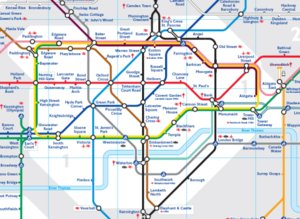
\includegraphics[height=\the\HauteurDesPhotos]{metro}&%
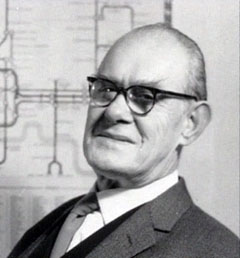
\includegraphics[height=\the\HauteurDesPhotos]{Beck}\\%
Carte&Beck%
\end{tabular}}
\medskip
\ImageAGauche{%
La représentation schématique généralement utilisée pour représenter un réseau de métro a été mise au point, la première fois, en 1931 par Henry Beck,\index[aut]{Beck (Henry Charles, dit Harry), 1902-1974, Anglais} alors dessinateur industriel de 29 ans et engagé comme intérimaire par la société du métro londonien.
Facile à comprendre et à utiliser, esthétique... elle est pourtant fausse à tous les égards sauf deux.\\
\indent Elle n'est pas à l'échelle, donc toutes les distances sont fausses; les lignes droites reliant les stations ne traduisent absolument pas le cheminement réel du métro sous les rues; les orientations sont fausses (une ligne verticale ne signifie pas que le trajet s'effectue selon l'axe nord-sud).\\
\indent Le premier aspect exact est que si une station de métro est représentée au nord de la Tamise, alors il en est de même pour la station réelle.
Le second aspect exact est la description du réseau: l'ordre des stations sur chaque ligne et les interconnexions entre les lignes sont fidèles à la réalité. C'est d'ailleurs ce second aspect qui est finalement le seul dont les voyageurs ont effectivement besoin.\\
\indent Notons enfin que cette illustration permet de comprendre aisément comment la notion de distance peut être appréhendée en topologie.
}
\end{histoire}

\medskip
\section{Petit exemple amusant d'injection dans un Hilbert}
Soient~$V$ et~$H$ deux espaces de Hilbert sur~$\RR$ et~$V$ inclus dans~$H$ avec injection continue et~$V$ dense dans~$H$.

\medskip
Comme~$V$ est inclus dans~$H$, l'injection est tout bêtement $i: x\mapsto x$.

\medskip
Dans ces conditions, $H$ est un espace de Hilbert avec un produit scalaire $(\ \mid\ )_H$, et $V$ muni du produit scalaire induit est un sous-espace dense, donc \textcolorred{ne peut pas être un espace de Hilbert} par restriction du produit scalaire $(\ \mid\ )_H$.
La structure hilbertienne de $V$ est définie par un produit scalaire $(\ \mid\ )_V$ propre à $V$.

\medskip
Il y a donc deux topologies sur $V$: la topologie hilbertienne propre à $V$ et la topologie héritée de la structure hilbertienne de $H$.
La continuité de l'injection $i$ impose donc une condition sur ces topologies: la topologie hilbertienne de $V$ est plus fine que la trace sur $V$ de la topologie hilbertienne de $H$.

\medskip
\textcolorgris{... et maintenant que le terme «injection» a été prononcé, il est temps
de passer au chapitre suivant...} 
% \include{./tex/Operat}
% \chapter{Continuité et dérivabilité}
\begin{abstract}
Dans ce chapitre, nous nous intéresserons aux notions de continuité et de
dérivabilité, les espaces nécessaires ayant été définis précédemment,
ainsi que les notions d'application...

Dans la mesure où les problèmes que nous souhaitons aborder, i.e. ceux issus de
la physique, sont généralement décrits par des équations différentielles ou des équations différentiellesP, on comprend bien
que la notion de dérivation est centrale.

Mais n'oublions pas que ces notions de continuité et de différentiabilité n'ont pas toujours
été définies de manière précise au cours de l'histoire et ont donné lieu à de bien
terribles affrontements entre nos glorieux anciens.
\end{abstract}



\medskip
\section{Continuité et classe~$C^0$}\index{Continuité!$C^0$}

\medskip
\begin{histoire}%
Dans le manuscrit de 1673 \emph{la Méthode inverse des tangentes ou à
propos des fonctions}, Leibniz\index[aut]{Leibniz (Gottfried Wilhelm), 1646-1716, Allemand} dit:
 <<~J'appelle fonctions toutes les portions des lignes droites
qu'on fit en menant des droites indéfinies qui répondent au point fixe et aux points de la courbe;
comme sont abscisse, ordonnée, corde, tangente, perpendiculaire, sous-tangente, sous-perpendiculaire...
et une infinité d'autres d'une construction plus composée, qu'on ne peut figurer.~>>
Finalement, au terme d'une correspondance nourrie entre Leibniz\index[aut]{Leibniz (Gottfried Wilhelm), 1646-1716, Allemand}
et Jean Bernoulli,\index[aut]{Bernoulli (Jean), 1667-1748, Suisse} celui-ci donne en 1718 la
définition suivante: <<~On appelle fonction d'une grandeur variable une quantité composée,
de quelque manière que ce soit, de cette grandeur variable et des constantes.~>>.
Il propose la notation~$\phi x$.

La continuité est en quelque sorte contenue, sous-jacente à ces définitions car
les fonctions considérées sont <<~physiques~>> et ne présentent au plus qu'un nombre
fini de discontinuités.

\sbox{\MaBoiteAvecPhotos}{\setlength{\tabcolsep}{0pt}\scriptsize%
\begin{tabular}{ccc}%
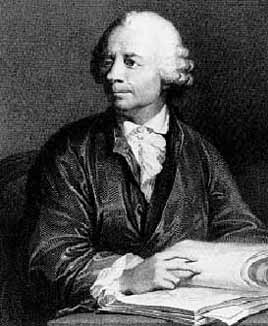
\includegraphics[height=\the\HauteurDesPhotos]{Euler3}&%
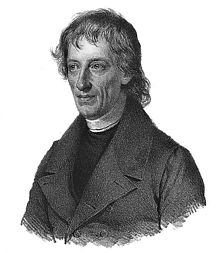
\includegraphics[height=\the\HauteurDesPhotos]{Bolzano}&%
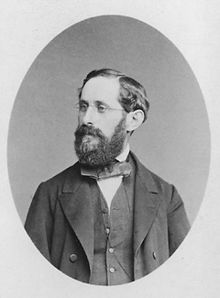
\includegraphics[height=\the\HauteurDesPhotos]{Heine}\\%
Euler &Bolzano&Heine%
\end{tabular}}
\medskip
\ImageADroite{%
Dans son \emph{Introductio in analysin infinitorum} de 1748, Euler\index[aut]{Euler (Leonhard Paul), 1707-1783, Suisse}
définit une fonction d'une quantité variable comme <<~une
expression analytique composée d'une manière quelconque de cette quantité
variable et de nombres ou de quantités constantes~>>. Le mot <<~analytique~>>
n'est pas davantage précisé.
En fait, pour Euler, une fonction\index[aut]{Euler (Leonhard Paul), 1707-1783, Suisse} est une
combinaison quelconque d'opérations prises dans le stock des opérations et
des modes de calcul connus de son temps, et applicables aux nombres:
opérations classiques de l'algèbre, exponentielle, logarithme, passage d'un
arc à ses lignes trigonométriques..., certaines de ces opérations pouvant être
itérées un nombre illimité de fois...}

Dans ce même ouvrage, Euler\index[aut]{Euler (Leonhard Paul), 1707-1783, Suisse}
dit qu'une fonction est continue si elle est définie par une seule expression anlytique
(finie ou infinie) et mixte ou discontinue si elle possède plusieurs expression analytiques
suivant ses intervalles de définition.
\medskip
La définition actuelle est celle due à Bernard Bolzano\index[aut]{Bolzano (Bernard Placidus Johann Nepomuk), 1781-1848, Allemand}
 dans sa théorie des
fonctions en 1816: <<~La fonction~$f(x)$ varie suivant la loi de continuité pour la valeur~$x$
si la différence~$| f(x + w) -f(x) |$ peut-être rendue plus petite que toute valeur donnée.~>>
Il existe une notion de continuité uniforme qui est plus forte que la simple continuité
et fixée par Heinrich Eduard Heine\index[aut]{Heine (Eduard), 1821-1881, Allemand}
 en 1872.
\end{histoire}
%\colorblack


\medskip
La continuité est une propriété topologique (donc indépendante de la métrique).

\medskip
\begin{definition}[Continuité d'une fonction en un point (version topologique)]
Soit~$f$ une application d'un espace topologique~$E$ dans un espace topologique
$F$.
On dit que \textcolorblue{$f$ est continue en un point}~$a$ de~$E$ si, quelque
soit le voisinage~$W$ de~$f(a)$ dans~$F$, il existe un voisinage~$V$ de~$a$ dans~$E$
tel que:
\begin{equation}
\forall x\in V, \quad f(x)\in W
\end{equation}
i.e. que l'image réciproque de tout voisinage de~$f(a)$ est un voisinage de~$a$.
\end{definition}

\textcolorgris{Cette définition est donnée pour la culture, car nous n'avons pas
rappelé la notion de voisinage dans ce document. Cela n'a pas d'importance
dans ce contexte puisque nous travaillerons sur des cas moins généraux.}

\medskip
Évidemment, une application de~$E$ dans~$F$ est \textcolorblue{continue} si
elle est continue en tout point de~$E$.

\medskip
Ramenons nous à des choses plus connues et plus en lien avec ce document.
Dans le cas des espaces métriques, la continuité se définit comme suit.

\begin{definition}[Continuité d'une fonction en un point (version métrique)]
Soient~$(E,d)$ et~$(E',d')$ deux espaces métriques, $f: E \to E'$ et~$a \in E$.
On dit que l'application~$f$ est continue en~$a$ si:
\begin{equation}
  \forall \varepsilon > 0, \quad \exists \eta > 0, \quad \forall x \in E, \quad \Bigl[d(x,a)<\eta \implies d'(f(x),f(a))<\varepsilon\Bigr]
\end{equation}
Ainsi~$f$ est continue en~$a$ si et seulement si la limite de~$f$ en~$a$ existe
(elle vaut alors nécessairement~$f(a)$).
\end{definition}

\medskip
Considérons la fonction~$f$ définie sur~$\RR^2$ par:
\begin{equation}
  f(x,y)=\left\{\begin{aligned}&\frac{xy}{x^2+y^2}&&\text{si~$(x,y)\neq(0,0)$} \\
&0&&\text{si~$(x,y)=(0,0)$} \end{aligned}\right.
\end{equation}
Elle n'a pas de limite en~$(0,0)$.

\colorgris\small
En effet, $f(x,y)$ est continue partout sur~$\RR^2\backslash\{(0,0)\}$.
Elle est continue sur l'axe des abscisses et des ordonnées où elle est~$\equiv0$.
Elle est donc séparément continue à l'origine, et par suite dans tout le plan.
Mais elle n'est pas continue par rapport à l'ensemble des variables à l'origine,
car sur la droite~$y=mx$, elle prend la valeur~$m/(1+m^2)$ en dehors de
l'origine; or~$\frac{m}{1+m^2}\ne0$ dès que~$m\ne0$, et par conséquent elle
ne tend pas vers~$0$ lorsque~$(x,y)$ tend vers l'origine.\colorblack
\normalsize

\medskip
\textcolorred{Pour une fonction réelle, on peut définir une fonction continue
comme une fonction dont on peut tracer le graphe sans lever le crayon}.
Si l'on exclut certains fonctions très particulières (comme les fractales), alors l'idée générale
de la continuité est bien traduite par cette phrase (la fonction ne présente pas de <<~saut~>>).

\medskip
%Définie de cette manière simple, une fonction~$f: I\subset\RR \to \RR$ sera dite \textcolorblue{continue
%au point~$a\in I$} si:
\begin{definition}[Continuité d'une fonction réelle en un point]
Une fonction~$f: I\subset\RR \to \RR$ sera dite \textcolorblue{continue
au point~$a\in I$} si:
\begin{equation}
  \forall \varepsilon > 0, \quad \exists \eta > 0, \quad \forall x \in I, \quad \Bigl[|x - a| <\eta \implies |f(x) - f(a)|<\varepsilon\Bigr].
\end{equation}
\end{definition}

\medskip
\textcolorblue{La classe des fonctions continues} est notée~$C^0$.
Elle inclut par exemple les fonctions continues par morceaux ainsi que les constantes (dont
la fonction nulle).

\medskip
Attention à ne pas confondre la classe des fonctions continues~$C^0$ avec
$C_0$ l'ensemble des fonctions continues qui s'annulent à l'infini (sous-espace de l'espace
des fonctions continues).

\medskip
\section{Continuité de Hölder et Lipschitz}\index{Continuité!Hölder}\index{Continuité!Lipschitz}%
\index[aut]{Hoelder@Hölder (Otto Ludwig), 1859-1937, Allemand}\index[aut]{Lipschitz (Rudolph Otto Sigismund), 1832-1903, Allemand}

\colorgreen\textbf{Remarque:}
Dans le cas des espaces métriques, nous avons vu qu'il était possible
de redéfinir la continuité à l'aide des~$\varepsilon$ plutôt que
par les voisinages.\vskip15pt

\sbox{\MaBoiteAvecPhotos}{\setlength{\tabcolsep}{0pt}\scriptsize%
\begin{tabular}{cc}%
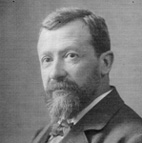
\includegraphics[height=\the\HauteurDesPhotos]{Holder}&%
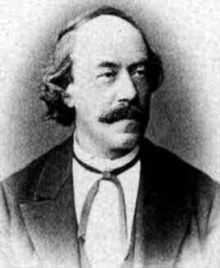
\includegraphics[height=\the\HauteurDesPhotos]{Lipschitz}\\%
Hölder &Lipschitz%
\end{tabular}}
\bigskip\ImageADroite{\colorgreen
Avec Hölder\index[aut]{Hoelder@Hölder (Otto Ludwig), 1859-1937, Allemand}
 et Lipschitz,\index[aut]{Lipschitz (Rudolph Otto Sigismund), 1832-1903, Allemand}
 la notion de <<~continuité uniforme~>> nous est proposée.
La distinction entre continuité et continuité uniforme est la même que celle entre la
convergence simple et la convergence uniforme dans le cas des séries (pour le lecteur
qui s'en souviendrait).
En effet, cette continuité uniforme ne regarde pas comment (quel~$\varepsilon$) la fonction
est continue en chaque point, mais comment elle est continue dans sa globalité, i.e.
lorsque ce fameux~$\varepsilon$ n'est plus lié à la position sur la courbe, mais est fixé
pour la fonction entière.}
\colorblack
\medskip
La \textcolorblue{continuité höldérienne} ou \textcolorblue{condition de Hölder}
est une condition suffisante (mais non nécessaire) pour qu'une application définie entre
deux espaces \textcolorred{métriques} soit continue.

La définition s'applique en particulier pour les fonctions d'une variable réelle.

\medskip
\begin{definition}[Fonction~$a$-höldérienne]
Si~$(E, d)$ et~$(F, d')$ sont deux espaces métriques, une fonction~$f: E \rightarrow F$ est dite
$a$-höldérienne s'il existe une constante~$C > 0$ telle que:
\begin{equation}
  \forall (x, y) \in \mathrm{e}^2,\quad d'\left(f(x), f(y)\right) \le C\,d\left(x,y\right)^a
\end{equation}
\end{definition}
\medskip
La continuité höldérienne d'une fonction dépend donc d'un paramètre réel
strictement positif~$a \in \intof{0}{1}$, et prend en compte toutes les variations de la valeur de
la fonction sur son ensemble de définition.
\medskip
Si~$0 < a \leq1$ est fixé, l'ensemble des fonctions réelles~$a$-höldériennes est un
espace vectoriel, conventionnellement noté~$\mathcal{C}^{0, a}(E,\RR)$.

\medskip
\begin{theoreme}
Toute application~$f$ qui est~$a$-höldérienne est continue. Mieux, elle est
\textcolorblue{uniformément continue}, dans le sens suivant:
\begin{equation}
\text{Si} \varepsilon>0\text{, alors pour} \eta = \left( \varepsilon / C \right)^{1 / a},\quad d\left( x, y \right) < \eta \ \Rightarrow\ d\left( f(x), f(y) \right) < \varepsilon
\end{equation}
Le réel~$\eta$ dépend de~$\varepsilon$ mais est indépendant de la variable~$x$
parcourant l'espace de définition de l'application.
\end{theoreme}
%%%#\bigskip
\begin{definition}[Fonction lipschitzienne]
Lorsque~$a = 1$, l'application est dit \textcolorblue{lipschitzienne}.
Une application lipschitzienne est plus <<~régulière~>> qu'une fonction
simplement continue.
\end{definition}
\medskip
Toute fonction lipschitzienne (en tant que fonction höldérienne) est uniformément continue.
\medskip
Toute fonction réelle lipschitzienne est (absolument continue donc à variation bornée donc)
dérivable presque partout pour la mesure de Lebesgue et sa dérivée est essentiellement bornée.
\medskip
\section{Dérivée}\index{dérivée!classique}
\medskip
\begin{definition}[Dérivée d'une fonction]
Soit~$f$ une application d'un ouvert~$\Omega$ du corps des scalaires~$\KK$ (resp. un invervalle
de~$\RR$) dans un espace affine normé~$F$ (resp.~$\RR$), alors on peut donner un sens,
pour~$a\in\Omega$ à la quantité:
\begin{equation}
f'(a)=\lim_{\substack{h\ne0\\h\to0\\a+h\in\Omega}} \dfrac{f(a+h)-f(a)}h \in F
\end{equation}
que l'on appelle le vecteur dérivé ou simplement la \textcolorblue{dérivée} de
$f$ en~$a$.
\end{definition}

\begin{histoire}%
Au XVIIe siècle, la compréhension mais surtout la modélisation (i.e. la mise en équations)
de phénomènes physiques et techniques conduit à la création au siècle suivant de
l'analyse en tant que branche des mathématiques
abordant les notions de dérivation, intégration et équations différentielles.

\sbox{\MaBoiteAvecPhotos}{\setlength{\tabcolsep}{0pt}\scriptsize%
\begin{tabular}{cc}%
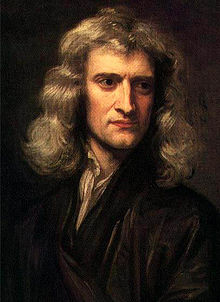
\includegraphics[height=\the\HauteurDesPhotos]{Newton}&%
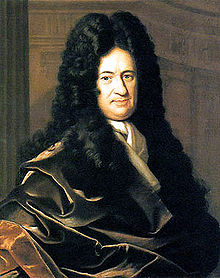
\includegraphics[height=\the\HauteurDesPhotos]{Leibniz}\\%
Newton &Leibniz%
\end{tabular}}
\medskip
\ImageADroite{%
Les échanges, les conceptions et la compréhension des infinitésimaux ont animé le monde scientifique
pendant bien longtemps, la discussion était tout autant philosophique que mathématique, ce
qui est somme toute assez normal compte tenu du sujet...
Les fondateurs incontestés de l'analyse sont Newton\index[aut]{Newton (Isaac, Sir -), 1643-1727, Anglais}
 et Leibniz.\index[aut]{Leibniz (Gottfried Wilhelm), 1646-1716, Allemand}
La portée de ces travaux est considérable car ils vont permettre non seulement la compréhension
des courbes (puis le calcul des aires), mais aussi celle du mouvement des corps.
C'est véritablement une révolution où l'on passe d'une science de la statique à une
science de la dynamique.
}

Un débat houleux sur la paternité du calcul différentiel entre mathématiciens britanniques et allemands
fit rage, mais Newton et Leibniz s'en tinrent à l'écart.
Toutefois, cette polémique entre les deux camps ne sera pas sans effet.
Celle-ci fera que les anglais resteront à l'écart du développement général des mathématiques
au XVIIIe siècle, la tradition newtonienne dominante ayant abouti à une certaine stagnation
scientifique. Au début du XIXe siècle, avec la diffusion des notations symboliques leibniziennes
du calcul infinitésimal, un petit groupe de mathématicien de Cambridge se mettront
à réfléchir sur le rôle et l'importance de la symbolique.

\medskip
L'opinion générale est aujourd'hui que Leibniz s'est presque
certainement inspiré de certaines des idées de Newton (dont les travaux sont antérieurs, mais non publiés au moment
où Leibniz publie), mais que sa contribution reste suffisamment importante pour que le
mérite de l'invention du calcul différentiel soit accordé aux deux hommes.

L'approche de Newton est proche de la physique: il parle en termes de mouvement physique et ses notations
ne sont employées que très rarement en dehors de la sphère des physiciens.

L'approche de Leibniz en revanche est plus géométrique et conduit à une présentation plus naturelle,
encore utilisée aujourd'hui, et qui va rapidement être adoptée en Europe. C'est lui également qui
introduit la notation~$dy/dx$ encore utilisée.

\sbox{\MaBoiteAvecPhotos}{\setlength{\tabcolsep}{0pt}\scriptsize%
\begin{tabular}{cc}%
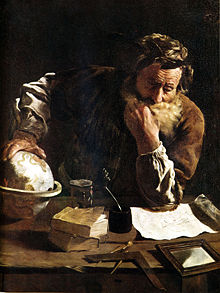
\includegraphics[height=\the\HauteurDesPhotos]{Archimede}&%
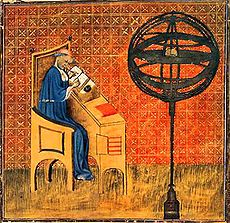
\includegraphics[height=\the\HauteurDesPhotos]{Oresme}\\%
Archimède&Oresme%
\end{tabular}}
\medskip
\ImageAGauche{%
Pourtant, si on regarde un peu plus dans l'Histoire, on peut dire que la méthode d'exhaustion,
telle qu'elle a été développée et utilisée par Archimède\index[aut]{Archimède de Syracuse, -287-- -212, Grec}
(i.e. avec toute la rigueur nécessaire, en usant du procédé d'encadrement évitant
le recourt aux~$\varepsilon$) est réellement la première utilisation des infinitésimaux.
Malgré, ou peut-être à cause de, la grande originalité de ses travaux, Archimède\index[aut]{Archimède de Syracuse, -287-- -212, Grec}
n'a été que peu suivi dans le monde grec et n'a pas eu de disciple direct.\\
\indent
Les savants arabes commenceront d'ailleurs dès le IXe siècle à s'intéresser aux procédés
infinitésimaux mis en œuvre par le génial Alexandrin.\\
\indent
Notons également que le plus grand progrès théorique réalisé au Moyen-Âge est l'étude
quantitative de la variabilité par Nicole Oresme\index[aut]{Oresme (Nicole), 1325-1382, Allemand}.
%(l'Einstein du XIVe siècle).
Éveillé par la diffusion des méthodes infinitésimales des Anciens, et d'Archimède\index[aut]{Archimède de Syracuse, -287-- -212, Grec}
en particulier, nourri par les spéculations scolastiques sur l'infini, le goût des
mathématiciens pour les considérations infinitésimales se développe peu à peu.
Ils s'appliquent d'abord à imiter le modèle archimédien, puis s'émancipent et essaient
de trouver des substituts pour la méthode d'exhaustion, jugée trop lourde.
}

\medskip
En 1748, Euler\index[aut]{Euler (Leonhard Paul), 1707-1783, Suisse}
 définit les deux nouvelles opérations que sont la différentiation et l'intégration
dans \emph{Introductio in analysin infinitorum}, puis dans \emph{Calculi differentialis} (1755) et
\emph{Institutiones calculi integralis} (1770) essaie de mettre au point les règles d'utilisation des
infiniment petits et développe des méthodes d'intégration et de résolution d'équations différentielles.
\end{histoire}
\colorblack

\medskip
La dérivabilité est elle-aussi une notion topologique et non métrique (même si on sait
l'écrire en termes métrique comme ci-dessus), elle ne dépend donc pas
de la norme choisie (du moment que celle-ci est compatible avec la topologie choisie...).

\medskip
\section{Fonctions de classe~$C^k$}\index{Continuité!$C^k$}
%%%%%%%%%%%%%%%%%%
\medskipvm
Il est évident que si la dérivée (telle que définie au dessus) existe partout dans
$\Omega$, alors on peut à nouveau considérer sa dérivée... et ainsi de suite.

On définit donc les \textcolorblue{classes~$C^1$, $C^2$, ...~$C^k$, ...~$C^\infty$}
de fonctions 1 fois, 2 fois, ..., $k$ fois continûment dérivables ou même indéfiniment
dérivables.
%%%%%%%%%%%%%%%%%%
\medskipvm
Pour~$k=0$, on retombe sur la définition de l'ensemble des fonctions
continues.
%%%%%%%%%%%%%%%%%%
\medskipvm
Pour être très clair, \textcolorred{une fonction est de classe~$C^k$ signifie que
toutes ses dérivées jusqu'à l'ordre~$k$ sont continues dans~$\Omega$}.
%%%%%%%%%%%%%%%%%%
\medskipvm
Toutes les fonctions polynomiales sont~$C^\infty$, car à partir d'un certain rang
leur dérivée est identiquement nulle.

\medskip
\section{Dérivées partielles}\index{dérivée!partielle}
Nous allons maintenant étendre la dérivation au cas où une fonction dépend
de plusieurs variables.
Évidemment, il faudra que dans le cas où la fonction ne dépend que d'une seule
variable, les deux notions coïncident.

\medskip
\textcolorblue{La dérivée partielle d'une fonction de plusieurs variables est la dérivée par rapport
à l'une de ses variables, les autres étant gardées constantes.}
%%%%%%%%%%%%%%%%%%
\medskipvm
La dérivée partielle de la fonction~$f$ par rapport à la variable~$x$ est notée
$\frac{ \partial f}{ \partial x}$ ou~$\partial_x f$ ou encore~$f'_x$.
%%%%%%%%%%%%%%%%%%
\medskipvm
De la même manière, on peut noter des dérivés secondes,...~$k$-èmes par
rapport à différentes variables.
Par exemple~$\frac{ \partial^2 f}{ \partial x^2} = f_{xx}' = \partial_{xx} f = \partial^2_x f$,
mais également~$\frac{ \partial^2 f}{\partial x\,\partial y} = f_{yx}' = \partial_{yx} f$, ou
$\frac{ \partial^2 f}{\partial y\,\partial x} = f_{xy}' = \partial_{xy} f~$, mais également
$\frac{ \partial^{i+j+k} f}{ \partial x^i\, \partial y^j\, \partial z^k} = f_{kz jy ix}' = \partial_{kz jy ix} f~$.

\medskip
\begin{definition}[Dérivée partielle d'ordre 1 en un point]
%La définition se fait de manière analogue au cas de la dérivée <<~classique~>>.
%
Soient~$\Omega$ un ouvert de~$\RR^n$ et~$f$ une fonction de~$n$ variables:
\begin{equation}
f: \begin{array}{ccc}
\Omega &\to& \RR\\
 \mathbf{x} = (x_1,\dots,x_n) &\mapsto& f(\mathbf{x}) = f(x_1,\dots,x_n)
\end{array}\end{equation}
On définit la \textcolorblue{dérivée partielle d'ordre 1 de~$f$ au point~$\mathbf{a} = (a_1,\dots,a_n) \in \Omega$
par rapport à la~$i$-ème variable~$x_i$} par:
\begin{equation}
  \frac{ \partial f}{\partial x_i}(\mathbf{a}) = \lim_{h \to 0}{ f(a_1, \dots , a_{i-1}, a_i+h, a_{i+1}, \dots ,a_n) - f(a_1, \dots ,a_n) \over h}
\end{equation}
\end{definition}

\medskip
\textcolorred{Attention:}
Même si toutes les dérivées partielles~$\frac{ \partial f}{\partial x_1}(\mathbf{a}),\, \dots,\, \frac{ \partial f}{\partial x_n}(\mathbf{a})$
existent en un point~$\mathbf{a}$, la fonction peut ne pas être continue en ce point.
Si l'on considère à nouveau la fonction~$f$ définie sur~$\RR^2$ par:
\begin{equation}
  f(x,y)=\left\{\begin{aligned}&\frac{xy}{x^2+y^2}&&\text{si~$(x,y)\neq(0,0)$}\\
&0&&\text{si~$(x,y)=(0,0)$}\end{aligned}\right.
\end{equation}
on voit qu'elle vérifie~$\frac{\partial f}{\partial x} (0,0)= \frac{\partial f}{\partial y} (0,0)=0$
mais elle n'a pas de limite en~$(0,0)$ comme nous l'avons vu avant.


\medskip
Si \textcolorred{toutes} les dérivées partielles (d'ordre 1) existent et sont \textcolorred{continues} dans
un voisinage de~$\mathbf{a}$, alors~$f$ est différentiable dans ce voisinage et la différentielle
est continue. Dans ce cas, on dit que~$f$ est une fonction de \textcolorblue{classe~$C^1$} sur ce
voisinage de~$\mathbf{a}$.

%%%#\bigskip
Si \textcolorred{toutes} les dérivées partielles secondes de~$f$ existent et sont \textcolorred{continues}
sur l'ouvert~$\Omega$, on dit que~$f$ est une fonction de \textcolorblue{classe~$C^2(\Omega)$}.
L'ordre de dérivation peut alors être changé sans que cela modifie le résultat.
C'est le \textcolorblue{théorème de Schwarz%\footnotemark
}.\index[aut]{Schwarz (Hermann Amandus), 1843-1921, Allemand}
\begin{theoreme}[Théorème de Schwarz]
Si~$f\in C^2(\Omega)$, alors:
\begin{equation}\colorred
  \frac{\partial^2f}{\partial x_i\, \partial x_j} = \frac{\partial^2f} {\partial x_j\, \partial x_i}
\end{equation}
\end{theoreme}
%\footnotetext{
%\begin{tabular}{c}
%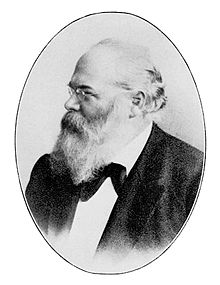
\includegraphics[height=32mm]{Schwarz}\\
%Hermann Amandus Schwarz\\
%1843-1921\\
%\end{tabular}
%}

%%%#\bigskip
\begin{definition}[Différentielle totale]
On appelle \textcolorblue{différentielle totale} de~$f$ l'expression:
\begin{equation}
  \dd f=\frac{\partial f}{\partial x_1}\,\dd x_1+\cdots+\frac{\partial f}{\partial x_n}\,\dd x_n
=  \dsum_i \frac{\partial f}{\partial x_i}\,\dd x_i
\end{equation}
\end{definition}

\medskip
\section{Retour sur les classes~$C^k$ pour une fonction de plusieurs variables}

Ce paragraphe met l'accent sur le cas multi-dimensionnel des classes~$C^k$
(ce qui est le cas avant, mais peut-être moins visiblement).
Nous en profitons également pour introduire des notations et notions dont nous
nous servirons plus loin.

\medskip
\begin{definition}[Fonctions~$k$ fois différentiables]
Si~$\Omega$ est un ouvert de~$\RR^n$, on définit l'ensemble des
fonctions~$k$ fois différentiables dans~$\Omega$, à valeurs
dans~$\RR$ dont toutes les dérivées jusqu'à l'ordre~$k$ sont continues dans
$\Omega$ par:
\begin{equation}
C^k(\Omega) = \left\{f\in C^{k-1}(\Omega), \dfrac{\partial f}{\partial x_i}\in C^{k-1}(\Omega),
i=1, ..., n\right\}, k\ge 1
\end{equation}
\end{definition}

\medskip
\begin{definition}[Multi-indice]
On appelle \textcolorblue{multi-indice}~$\alpha$ un~$n$-uplet d'entiers
$\alpha=(\alpha_1, ..., \alpha_n)$, $\alpha_j\in\NN$.
Sa \textcolorblue{longueur} est~$|\alpha|=\alpha_1+ ... + \alpha_n$,
et on note \textcolorblue{$\partial^\alpha$} la quantité (l'opération)
\begin{equation}\partial^\alpha=\left(\dfrac{\partial}{\partial x_1}\right)^{\alpha_1}...\left(\dfrac{\partial}{\partial x_n}\right)^{\alpha_n}\end{equation}
\end{definition}

\medskip\colorgris
$C^k(\Omega)$ est l'espace vectoriel des fonctions~$f: \Omega \to \RR$ telles que
$\forall \alpha$, $|\alpha|\le k$, $x\mapsto \partial^\alpha f(x)$ existe et appartient
à~$C^0(\Omega)$.

Pour~$f$ et~$g$ dans~$C^k(\Omega)$, on définit:
\begin{equation}
d(f,g)=\dsum_{i=1}^\infty \dfrac1{2^i}\dfrac{\dsum_{|\alpha|\le k} \sup_{K_i}|\partial^\alpha f(x)-g(x)|}{%
1+\dsum_{|\alpha|\le k} \sup_{K_i}|\partial^\alpha f(x)-g(x)|}
\end{equation}
qui est une distance sur~$C^k(\Omega)$ qui en fait un espace complet. L'espace~$C^\infty(\Omega)$ peut se définir par: \begin{equation} C^\infty(\Omega)=\bigcup\limits_{k\in\NN}C^k(\Omega)\end{equation}
qui est également complet pour la même distance.
%\textcolorblue{Cette définition permet de clairement voir les inclusions successives des espaces~$C^k$.}

\bigskip\colorblack
On définit également~$C^k_b(\Omega)$ comme le sous-espace vectoriel des éléments
de~$C^k(\RR^n)$ dont \textcolorblue{toutes les dérivées jusqu'à l'ordre~$k$ sont bornées}
sur~$\Omega$.

On définit alors:
\begin{equation}
\|f\|_{C^k_b(\Omega)}=\dsum_{|\alpha|\le k} \sup_{\Omega} |\partial^\alpha f(x)|
\end{equation}
qui est une norme sur~$C^k_b(\Omega)$ et en fait un espace de Banach (i.e. normé
complet pour cette norme).

\medskip
\begin{definition}\label{Def-Cc}
On définit, pour~$k\in\NN\cup\{\infty\}$, l'ensemble \textcolorblue{$C_c^k(\Omega)$} par:
$f\in C_c^k(\Omega)$ si~$f\in C^k(\Omega)$ et si~$f$ est de support compact inclus dans~$\Omega$.
\end{definition}

Pour tout ouvert~$\Omega$ de~$\RR^n$, et pour tout~$k\in\NN\cup\{\infty\}$:
\begin{itemize}
  \item~$C_c^k(\Omega)$ est dense dans~$C^k(\Omega)$
  \item~$C_c^\infty(\Omega)$ est dense dans~$C^k(\Omega)$
\end{itemize}

\medskip
\section{Nabla et comparses}
\subsection{Champs de vecteurs et de scalaires}
\begin{definition}[Champ de vecteurs]
Soit~$E$ un espace vectoriel euclidien\index[aut]{Euclide, -325-- -265, Grec}
de dimension~$n$ et~$\Omega$ un ouvert de E.
Un \textcolorblue{champ de vecteurs} sur~$\Omega$ est une application~$F$ de~$\Omega$ dans~$E$,
définie par ses~$n$ fonctions composantes:
\begin{equation}
  F: \VV*{x_1\\\vdots\\x_n} \longmapsto \VV*{F_1(x_1,\dots,x_n)\\ \vdots\\ F_n(x_1,\dots,x_n)}
\end{equation}
C'est donc une fonction qui à un vecteur fait correspondre un vecteur.
\end{definition}
\medskip
\begin{definition}[Champ de scalaires]
Un \textcolorblue{champ de scalaires} sur~$\Omega$ est une application~$f$ de~$\Omega$ dans~$\RR$ ou~$\CC$,
i.e. une fonction qui à un vecteur fait correspondre un scalaire.
\end{definition}
La dérivée d'un champ scalaire est un champ vectoriel appelé \textcolorblue{gradient} (voir plus bas).

\medskip
\colorblue Nabla, noté~$\nabla$, est un pseudo-vecteur \colorblack servant à noter un opérateur
différentiel:
\begin{equation}
\nabla = \VV*{{\dfrac\partial{\partial x}}\\ \dfrac\partial{\partial y}\\ \dfrac\partial{\partial z}}_{\text{cartésiennes}}
= \VV*{\dfrac\partial{\partial \rho}\\ \dfrac1\rho \dfrac\partial{\partial \varphi}\\ \dfrac\partial{\partial z}}_{\text{polaires}}
= \VV*{\dfrac\partial{\partial r}\\ \dfrac1r \dfrac\partial{\partial \theta}\\\dfrac1{r\sin\theta} \dfrac\partial{\partial \varphi}}_{\text{sphériques}}
\end{equation}

\medskip
\subsection{Gradient, divergence, rotationnel, Laplacien et D'Alembertien}\index{Gradient}\index{divergence}\index{Rotationnel}\index{Laplacien}\index{D'Alembertien}
Les quantités présentées ci-après apparaîtront constamment dans les
problèmes physiques.%\footnote{
%\begin{tabular}{ccc}
%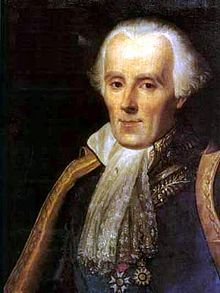
\includegraphics[height=32mm]{Laplace}&
%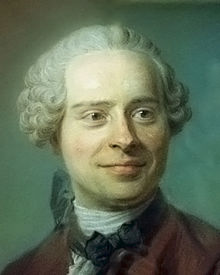
\includegraphics[height=32mm]{dAlembert}\\
%Pierre-Simon de Laplace &
%Jean le Rond D'Alembert\\
%1749-1827 &
%1717-1783\\
%\end{tabular}
%}



\medskip
Soient~$\mathbf{A}~$ un champ de vecteur et~$f$ un champ scalaire, on définit:
\begin{itemize}
\item Le \textcolorblue{gradient}:
\begin{equation} \gradb f \equiv \nabla f \end{equation}

\item La \textcolorblue{divergence}:
\begin{equation} \dive \mathbf{A} \equiv \nabla\cdot\mathbf{A} \end{equation}

\item Le \textcolorblue{rotationnel}:
\begin{equation} \rotb {\mathbf{A}} \equiv \nabla \wedge \mathbf{A} \end{equation}

\item Le \textcolorblue{Laplacien} (scalaire et vectoriel):
\begin{align} &\Delta f = \nabla^2 f\\
&\Delta \mathbf{A} = \nabla^2 \mathbf{A} \end{align}

\item Le \textcolorblue{D'alembertien}: il s'agit plus d'une <<~contraction d'écriture~>>.
En coordonnées cartésiennes, $\Box$ s'écrit:
\begin{equation}
  \Box = \frac{1}{c^2}\frac{\partial^2}{\partial t^2} - \left(\frac{\partial^2}{\partial x^2} + \frac{\partial^2}{\partial y^2} + \frac{\partial^2}{\partial z^2}\right)
  = \frac{1}{c^2}\frac{\partial^2}{\partial t^2} - \Delta
\end{equation}
\end{itemize}
où~$c$ est la vitesse de la propagation considérée (ou la vitesse de la lumière).

\medskip
En coordonnées cartésiennes, il vient explicitement:
\begin{itemize}
  \item gradient:~$ \gradb f=
	\VV*{{\partial f \over \partial x}\\ {\partial f \over \partial y}\\ {\partial f \over \partial z}}$
  \item divergence:~$ \dive \mathbf{A} =
	{\partial A_x \over \partial x} + {\partial A_y \over \partial y} + {\partial A_z \over \partial z}$
  \item rotationnel:~$ \rotb {\mathbf{A}} =
	\VV*{{\partial A_z \over \partial y} - {\partial A_y \over \partial z} \\
	{\partial A_x \over \partial z} - {\partial A_z \over \partial x} \\
	{\partial A_y \over \partial x} - {\partial A_x \over \partial y}}$
  \item Laplacien scalaire:~$\Delta f ={\partial^2 f \over \partial x^2} + {\partial^2 f \over \partial y^2} + {\partial^2 f \over \partial z^2}$
  \item Laplacien vectoriel:~$\Delta \mathbf{A} =
	\VV*{\Delta A_x \\ \Delta A_y \\ \Delta A_z}$
\end{itemize}

\medskip
De plus:
\begin{align}
&\dive \gradb f = \nabla \cdot (\nabla f) = \nabla^2 f = \Delta f\\
&\rotb\gradb f = \nabla \wedge ( \nabla f)
\colorred = \boldsymbol 0\\
&\dive\rotb \mathbf{A} = \nabla \cdot ( \nabla \wedge \mathbf{A} ) \colorred = 0\\
&\rotb\rotb\mathbf{A} = \nabla \wedge (\nabla \wedge \mathbf{A} ) =\nabla ( \nabla \cdot \mathbf{A} ) - \nabla^2 \mathbf{A} = \gradb\dive \mathbf{A} - \Delta \mathbf{A} \\
&\Delta f g = f \Delta g + 2 \nabla f \cdot \nabla g + g \Delta f
\end{align}

\medskip
\subsection{Normale et dérivée normale}\index{dérivée!normale}\index{Normale}

\begin{definition}[Normale]
On appelle \textcolorblue{normale} au domaine~$\Omega$ un champ de vecteurs
$n(x)$ défini sur le bord~$\Gamma=\partial\Omega$ de~$\Omega$ et tel qu'en tout point
$x\in\Gamma$ où le bord est régulier, $n(x)$ soit orthogonal au bord
et de norme~$1$.
\end{definition}

\medskip
On appelle \textcolorblue{normale extérieure} une normale qui pointe vers
l'extérieur du domaine en tout point.

\medskip
\begin{definition}[Dérivée normale]
On appelle \textcolorblue{dérivée normale} d'une fonction régulière~$u$
sur~$\Gamma$, la fonction définie sur les points réguliers de~$\Gamma$ par:
\begin{equation}\dfrac{\partial u}{\partial n}(x)=\nabla u(x)\cdot n(x)\end{equation} Il s'agit d'un produit
scalaire car~$\nabla u$ est un vecteur, tout comme~$n(x)$.
\end{definition}

\medskip
\subsection{Potentiel d'un champ vectoriel}

Le \textcolorblue{potentiel d'un champ vectoriel} est une fonction scalaire ou vectorielle qui,
sous certaines conditions relatives au domaine de définition et à la régularité,
permet des représentations alternatives de champs aux propriétés particulières.
Ainsi:
\begin{itemize}
  \item Un champ vectoriel irrotationnel (de rotationnel nul) peut être identifié au gradient d'un potentiel scalaire.
  \item Un champ vectoriel solénoïdal (de divergence nulle) peut être identifié au rotationnel d'un potentiel vecteur.
\end{itemize}
Dans les deux cas, on dit que le champ d'origine \textcolorblue{dérive d'un potentiel}
(allusion entre une fonction et sa primitive).

\medskip
Ces potentiels permettent non seulement d'appréhender certains champs vectoriels sous un angle
complémentaire (pour un traitement parfois plus aisé), mais ils légitiment des abstractions essentielles
comme, par exemple en physique, l'énergie potentielle associée à un champ de forces conservatives.

\medskip
Un champ de vecteurs~$\mathbf{A}~$ continu et irrotationnel dérive d'un potentiel scalaire~$U$:
\begin{equation}
 \mathbf{A} = -\gradb U
\end{equation}
Le même résultat se vérifie dans l'espace entier à condition que, vers l'infini, le champ
décroisse <<~assez~>> rapidement.

Le potentiel scalaire n'est pas unique, il est défini à une constante près.

\medskip
Un champ de vecteurs~$\mathbf{A}~$ régulier et de divergence nulle dérive d'un potentiel vectoriel
$\mathbf{B}~$:
\begin{equation}
  \mathbf{A} = -\rotb \mathbf{B}
\end{equation}
Le même résultat se vérifie dans l'espace entier à condition que, vers l'infini, le champ
décroisse <<~assez~>> rapidement.

Le potentiel vecteur n'est pas unique, il est défini à un <<~gradient~>> près (i.e.
$ \mathbf{B} ' = \mathbf{B} + \gradb f$ convient
également).

\medskip
\subsection{Signification <<~physique~>>}

Un \textcolorgreen{champ de scalaires}, c'est un <<~truc~>>, une application, qui à un vecteur
associe un scalaire. Typiquement, on peut penser à la \textcolorgreen{température}.
Une application~$T(x,y,z)$ qui à chaque point de l'espace de coordonnées~$(x,y,z)$ associe
sa température~$T$ est un champ de scalaire.

Un \textcolorgreen{champ de vecteurs}, c'est un <<~truc~>>, une application, qui à un vecteur
associe un autre vecteur. Typiquement, on peut penser à la \textcolorgreen{vitesse}.
Une application~$\mathbf{V}(x,y,z)$ qui à chaque point de l'espace de coordonnées~$(x,y,z)$
associe son vecteur vitesse~$\mathbf{V}$ est un champ de vecteurs.

\medskip
Si~$f$ est une fonction de classe~$C^1$, alors le \textcolorgreen{gradient} de~$f$ au point~$\mathbf{a}$,
quand il est non nul, s'interprète comme la direction selon laquelle~$f$ varie le plus vite,
i.e. la ligne de plus grande pente.

La \textcolorgreen{divergence} d'un champ de vecteurs mesure comment son courant déforme
un volume \textcolorgris{(on devrait dire comment son flot déforme une forme volume au sens
de la géométrie différentielle)}.
{\small L'idée est un peu la suivante: imaginons un écoulement de fluide et intéressons-nous au
courant en fonction de la profondeur. Lorsque l'on est un peu en dessous de la surface et loin
du sol, on peut imaginer que le courant est à peu près constant, donc une section (ou un volume)
de fluide perpendiculaire à l'écoulement se retrouve, un instant plus tard, un peu plus
loin, mais toujours perpendiculaire au sol, i.e. la section n'a pas varié.
Si l'on est proche du fond, on peut penser que le courant est plus faible très près du
sol, par exemple à cause du frottement. Si l'on considère à nouveau une section
de fluide perpendiculaire au sol, alors un instant plus tard, elle n'est plus perpendiculaire
au sol: près du sol, les particules ont effectué un petit déplacement, celles plus éloignées ont
beaucoup plus avancé. La section n'a ni la même forme, ni la même longueur
qu'à l'instant précédent. La divergence mesure justement ce type d'écart.}
\textcolorgreen{D'une manière plus générale, la divergence traduit la conservation (si elle
est nulle) ou non d'une grandeur physique en un point: cela mesure donc, en chaque point
si une grandeur (par exemple le volume comme avant) est conservative ou non.}


Le \textcolorgreen{rotationnel} exprime la tendance qu'ont les lignes de champ d'un champ vectoriel
à tourner autour d'un point: sa circulation locale sur un petit lacet entourant ce point est non nulle
quand son rotationnel ne l'est pas (nous n'avons pas défini la notion de lacet, nous compterons
sur l'imagination du lecteur). \textcolorgris{On rappelle que les lignes de champ sont les
lignes qui, en première approche, représente le chemin que l'on suivrait en partant d'un point.
Ce sont en fait les lignes orthogonales aux équipotentielles, ou surfaces de niveau, du champ.}

\medskip
Concernant le \textcolorgreen{Laplacien scalaire}, la quantité~$\Delta f$ est une mesure de la
différence entre la valeur de~$f$ en un point quelconque~$P$ et la valeur moyenne~$\overline{f}$
au voisinage du point~$P$.

Le \textcolorgreen{Laplacien scalaire} d'une fonction peut aussi être interprété comme la
courbure moyenne locale de la fonction, que l'on visualise aisément pour une fonction à
une seule variable~$f(x)$.
La dérivée seconde (ou courbure)~$f''$ représente la déviation locale de la moyenne par
rapport à la valeur au point considéré.


\bigskip
Les notions de rotationnel, gradient, Laplacien... interagissent. Par exemple en
\textcolorgreen{mécanique des fluides}, le rotationnel de la vitesse décrit une rotation de la particule fluide.
Si l'écoulement est irrotationnel (son rotationnel est nul en tout point), alors le vecteur vitesse est le gradient du
potentiel (on dit alors que les vitesses dérivent d'un potentiel).
Si le fluide peut être considéré comme incompressible, la divergence de ce vecteur s'annule.
Le laplacien du potentiel est donc nul: il s'agit d'un potentiel harmonique qui satisfait l'équation de Laplace.

\medskip
\section{Quelques théorèmes sur les intégrales}

Les relations ci-après permettent de passer d'intégales sur un domaine à des
intégrales sur le bord de ce domaine.


\medskip
\begin{theoreme}[Théorème du gradient]\index{Gradient}\index{théorème!du gradient}

Ce théorème met en relation l'intégrale de volume du gradient d'un champ scalaire et l'intégrale
de surface de ce même champ:
 \begin{equation}
  \int_\Omega \nabla f = \int_\Gamma f \vect{n}(x)
\end{equation}
où~$\Gamma$ est le bord du domaine~$\Omega$ et~$f$ un champ scalaire (i.e. une fonction régulière).
\end{theoreme}

\medskip
\begin{theoreme}[Théorème du rotationnel]\index{Rotationnel}\index{théorème!du rotationnel}

Ce théorème met en relation l'intégrale de volume du rotationnel d'un champ vectoriel et l'intégrale
de surface du même champ:
\begin{equation}
\int_\Omega \rotb {\mathbf{A}} =
-\int_\Gamma {\mathbf{A}} \wedge \vect{n}(x)
\end{equation}
où~$\Gamma$ est la frontière de~$\Omega$, $\wedge$ est le produit vectoriel et~$n(x)$ est
la normale dirigé vers l'extérieur.
\end{theoreme}

\medskip\colorgris
Une autre identité remarquable met en relation l'intégrale de surface du rotationnel d'un champ vectoriel
et l'intégrale curviligne (ou circulation) du même champ sur la frontière.
Elle découle du théorème de Green qui, pour une surface~$S$ (généralement non fermée) de
frontière~$C$, implique:
\begin{equation}
\iint_S \rotb {\mathbf{A}} \cdot \dd\mathbf{s} = \oint_C {\mathbf{A}} \cdot \dd\mathbf{l}
\end{equation}
Si~$S$ est fermée, $C$ est vide (ou réduit à un point) et le membre de droite est nul.

\medskip
L'orientation de la surface et celle de la courbe frontière sont liées puisque le changement
d'une orientation modifie le signe de l'intégrale correspondante.
En fait, la relation est satisfaite lorsque ces orientations sont telles que, sur un point frontère,
le vecteur tangent à la surface~$\dd \vec s \wedge \dd \vec l$ est orienté
en direction de la surface.
\colorblack


\medskip
\begin{theoreme}[Théorème de Green--Riemann]\index{théorème!de Green--Riemann}%
\index[aut]{Green (George), 1793-1841, Anglais}\index[aut]{Riemann (Georg Friedrich Bernhard), 1826-1866, Allemand}

Ce théorème donne la relation entre une intégrale curviligne autour d'une courbe simple fermée~$C$ et l'intégrale double sur la région du plan~$S$ délimitée par~$C$.

Soit~$C$, une courbe plane simple, positivement orientée et~$C^1$ par morceaux, $S$ le domaine compact lisse du plan délimité par~$C$ et 
$P\dd x + Q\dd y$ une 1-forme différentielle sur~$\RR^2$. Si~$P$ et~$Q$ ont des dérivées partielles continues sur une région ouverte incluant~$S$, alors:
\begin{equation}
\int_C P\,\dd x + Q\,\dd y = \iint_S \left( \frac{\partial Q}{\partial x} - \frac{\partial P}{\partial y}\ \right) \dd x\dd y
\end{equation}
\end{theoreme}

\medskip\colorgris
Il existe une autre façon de noter ce théorème.
On se place sur un domaine compact lisse du plan~$\Omega$, de bord~$\partial\Omega$,
en notant la forme différentielle~$\omega$.
Alors la dérivée extérieure de~$\omega$ s'écrit:
\begin{equation}
\dd \omega = \left( \frac{\partial Q}{\partial x} - \frac{\partial P}{\partial y} \right) \dd x \wedge \dd y
\end{equation}

On peut alors résumer le théorème de Green par la formule:
\begin{equation}
\oint_{\partial \Omega} \omega = \iint_{\Omega} \dd\omega
\end{equation}
(Le cercle sur l'intégrale précise que le bord décrit une courbe fermée).
\colorblack

\medskip
\begin{theoreme}[Théorème de Green-Ostrogradsky (flux-divergence)]\index[aut]{Green (George), 1793-1841, Anglais}%
\index[aut]{Ostrogradsky (Mikhaïl Vassilievitch), 1801-1862, Ukainien}\index{théorème!de Green-Ostrogradsky}%
\index{théorème!du flux-divergence}
(<<~Ostrogradsky~>> peut s'écrire avec un <<~y~>> ou un <<~i~>> à la fin.)
\medskip
\index{divergence}

Soit~$\Omega$ un domaine de~$\RR^2$ ou~$\RR^3$ de frontière~$\Gamma$
et~${\mathbf{A}}$ un champ de vecteurs:
\begin{equation}
  \int_\Omega \dive\ {\mathbf{A}} = \int_\Gamma {\mathbf{A}}\cdot n
\end{equation}
\end{theoreme}

\medskip
Ce théorème prend aussi le nom de théorème du flux-divergence ou plus simplement formule de la
divergence.

\begin{theoreme}[Formule de Green]
Du théorème de Green-Ostrogradsky on peut déduire la formule de Green:\index[aut]{Green (George), 1793-1841, Anglais}
soit~$\Omega$ un domaine de~$\RR^2$ ou~$\RR^3$ de frontière~$\Gamma$
et~$u$ et~$v$ deux fonctions régulières:
\begin{equation}
  \int_\Omega (\Delta u)v = -\dint_\Omega \nabla u\cdot\nabla v + \dint_\Gamma \dfrac{\partial u}{\partial n}v
\end{equation}
\end{theoreme}

\medskip
On en déduit certaines formules utiles du calcul vectoriel.
Soit~$\Omega$ un domaine de~$\RR^2$ ou~$\RR^3$ de frontière~$\Gamma$,
${\mathbf{A}}$ et~${\mathbf{B}}$ des champ de vecteurs, $f$ et~$g$ des
fonctions régulières, et~$n(x)$ la normale extérieure au point considéré:
\begin{align}
  &\int_\Omega \left( {\mathbf{A}}\cdot \nabla f + f \left(\nabla \cdot {\mathbf{A}}\right)\right)=
  \int_\Gamma f {\mathbf{A}}\cdot n(x)\\
&\int_\Omega \left( {\mathbf{B}}\cdot\left(\nabla \wedge {\mathbf{A}}\right) - {\mathbf{A}}\cdot \left(\nabla
\wedge {\mathbf{B}}\right) \right)
= \int_\Gamma \left({\mathbf{A}} \wedge {\mathbf{B}}\right)\cdot n(x)\\
&\int_\Omega \left( f \nabla^{2} g + \nabla f \cdot \nabla g \right)
= \int_\Gamma f \nabla g \cdot \vect{n}(x)
\end{align}
Ces formules sont exploitées pour obtenir des formulations faibles associées à des problèmes aux dérivées partielles. 
% \chapter{Espaces de Lebesgue}\label{Ch-Lp}
\begin{abstract}
Les espaces~$L^p$ sont indispensables à la définition des espaces de Sobolev après lesquels nous courons depuis quelques chapitres.

La mesure de Lebesgue a été introduite, les notions d'application et de continuité ont été rappelées... nous en avons plus qu'il ne nous en faut pour définir de tels espaces.
\end{abstract}
Comme promis au paragraphe~\ref{Sec-impasse}, nous fournissons maintenant quelques compléments sur l'intégration. Nous avons mentionné la mise en défaut de l'intégrale de Riemann\index[aut]{Riemann (Georg Friedrich Bernhard), 1826-1866, Allemand} dans le cas de l'indicatrice des rationnels.
Ce contre-exemple a été historiquement fourni par Dirichlet.\index[aut]{Dirichlet (Johann Peter Gustav Lejeune), 1805-1859, Allemand}, et on appelle encore cette fonction, fonction de Dirichlet.
Regardons toutefois d'un peu plus près d'où tout cela provient.

\medskip
\begin{histoire}%
Dans le chapitre VI, «Développement d'une fonction arbitraire en séries trigonométriques» de sa \emph{Théorie analytique}, Fourier\index[aut]{Fourier (Jean Baptiste Joseph), 1768-1830, Français} considère une fonction~$f$ définie dans~$]-\pi/2,+\pi/2[$ dont le développement en série trigonométrique est de la forme:
\begin{equation} f(x)=a_1\sin x+a_2\sin 2x +\ldots+a_k\sin kx +\ldots\end{equation}
\sbox{\MaBoiteAvecPhotos}{\setlength{\tabcolsep}{0pt}\scriptsize%
\begin{tabular}{c}%
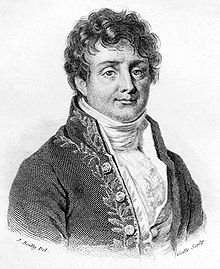
\includegraphics[height=\the\HauteurDesPhotos]{Fourier}\\
Fourier%
\end{tabular}}
%\medskip
\ImageAGauche{%
Le problème est de calculer les coefficients~$a_k$ dans le cas même, dit-il, où «la fonction~$f(x)$ représente une suite de valeurs ou ordonnées dont chacune est arbitraire... On ne suppose point que ces coordonnées soient assujetties à une loi commune; elles se succèdent d'une manière quelconque et chacune d'elles est donnée comme le serait une seule quantité».\\ \indent
On notera au passage que la fonction considérée par Fourier\index[aut]{Fourier (Jean Baptiste Joseph), 1768-1830, Français} n'est définie que par la donnée de ses points (si en plus ils sont en nombre fini, cela représente alors un échantillonnage). %\\ \indent
%
Fourier\index[aut]{Fourier (Jean Baptiste Joseph), 1768-1830, Français} conduit son calcul selon une voie nouvelle: en multipliant l'expression précédente par~$\sin kx$ et en intégrant terme à terme la série, mais sans justification, il obtient:
\begin{equation}a_k=\frac2{\pi}\dint_0^{\pi} f(x)\sin kx \dd x\end{equation}
Fourier\index[aut]{Fourier (Jean Baptiste Joseph), 1768-1830, Français} observe que dans tous les cas envisagés, ces intégrales ont un sens et en conclut que toute fonction d'une variable peut-être représentée par une série trigonométrique. }
Même manquant de rigueur, Fourier,\index[aut]{Fourier (Jean Baptiste Joseph), 1768-1830, Français} aboutit à un résultat juste pour les fonctions qu'il considère.
Or les fonctions considérées en l'occurrence «vont bien» pour l'intégrale de Riemann\index[aut]{Riemann (Georg Friedrich Bernhard), 1826-1866, Allemand} telle qu'elle est définie.

\medskip
\index[aut]{Riemann (Georg Friedrich Bernhard), 1826-1866, Allemand}
\begin{definition}[Intégrale de Riemann]
Soit~$f$ une fonction réelle définie sur un intervalle~$\intff{a}{b}$.
On considère une suite~$(x_i)$, $0\le i\le n$ de subdivisions de cet intervalle:
$a=x_0 < x_1 <\ldots < x_{n-1} <x_n=b$.
Notons~$\delta_i=x_i-x_{i-1}$ et~$S=\delta_1f(a+\varepsilon_1\delta_1) +
\delta_2 f(x_1+\varepsilon_2\delta_2)+ \ldots + \delta_nf(x_{n-1}+\varepsilon_n\delta_n)$,
où~$0\le \delta_i\le 1$.

Si la somme~$S$ a la propriété, de quelque manière que les~$\delta$ et les
$\varepsilon$ puissent être choisis, de s'approcher indéfiniment d'une limite fixe~$A$,
quand les~$\delta$ tendent vers zéro, cette limite s'appelle la valeur de l'intégrale
définie~$\int_a^b f(x)\dd x$.
\end{definition}
En termes modernes, on dira que pour qu'une fonction bornée soit Riemann-intégrable,\index[aut]{Riemann (Georg Friedrich Bernhard), 1826-1866, Allemand}
il faut et il suffit que l'ensemble des points de discontinuité de~$f$ soit de mesure nulle.
\medskipvm
\textcolorgris{En complément, on rappellera également que l'intégrale de Riemann n'est que la généralisation
de celle de Cauchy:\index[aut]{Cauchy (Augustin Louis, baron -), 1789-1857, Français} la valeur retenue pour calculer
la fonction sur chaque sous-intervalle n'est plus celle du point de gauche, mais peut être prise n'importe où dans ledit sous-intervalle.}

\sbox{\MaBoiteAvecPhotos}{\setlength{\tabcolsep}{0pt}\scriptsize%
\begin{tabular}{ccc}%
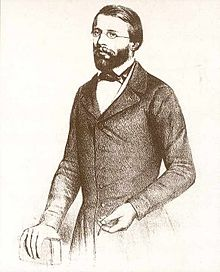
\includegraphics[height=\the\HauteurDesPhotos]{Riemann}&
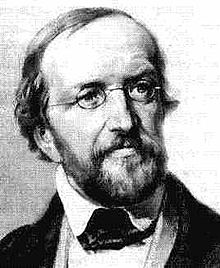
\includegraphics[height=\the\HauteurDesPhotos]{Dirichlet}&
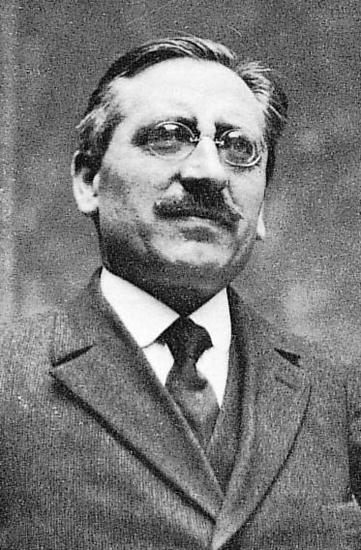
\includegraphics[height=\the\HauteurDesPhotos]{Lebesgue2}\\
Riemann&Dirichlet&Lebesgue%
\end{tabular}}
\medskip
\ImageADroite{%
Dès la fin de son mémoire de 1829, \emph{Sur la convergence des séries trigonométriques qui servent à représenter une fonction arbitraire entre des limites données}, Dirichlet\index[aut]{Dirichlet (Johann Peter Gustav Lejeune), 1805-1859, Allemand} donne l'exemple, d'une nature toute nouvelle, d'une fonction discontinue en tous ces points: la fonction~$f(x)$ qui vaut une constante~$c$ si~$x$ est un rationnel et qui vaut une autre constante~$d$ si~$x$ est irrationnel.
On voit alors directement que la Riemann-intégrabilité est mise à mal.\index[aut]{Riemann (Georg Friedrich Bernhard), 1826-1866, Allemand} Le travail consistera alors à définir précisément ce que l'on peut négliger, i.e. les parties de mesure nulle.}

\medskip
Lebesgue\index[aut]{Lebesgue (Henri-Léon), 1875-1941, Français} va commencer par définir un \textcolorblue{ensemble mesurable}: c'est un ensemble dont la mesure extérieure (i.e. la borne inférieure de la mesure des ouverts le contenant) est égale à sa mesure intérieure (i.e. la borne supérieure de la mesure des fermés qu'il contient): est-il besoin de rappeler la différence entre borne inférieure et minimum et entre borne supérieure et maximum ? La borne supérieure (ou le supremum) d'une partie d'un ensemble partiellement ordonné est le plus petit de ses majorants. Une telle borne n'existe pas toujours, mais si elle existe alors elle est unique. Elle n'appartient pas nécessairement à la partie considérée.
Dualement, la borne inférieure (ou l'infimum) d'une partie est le plus grand de ses minorants...

\textcolorblue{L'intégrale de Lebesgue}\index[aut]{Lebesgue (Henri-Léon), 1875-1941, Français} peut être définie de manière géométrique: pour une fonction positive~$f$ définie sur~$\intff{a}{b}$, elle est égale à la mesure de dimension deux de l'ensemble $\{(x,y)\in\RR^2 / a\le y\le f(x), a\le x\le b\}$ quand cette mesure existe.
D'une manière analytique, cette définition de l'intégrale de Lebesgue devient:\index[aut]{Lebesgue (Henri-Léon), 1875-1941, Français}

\begin{definition}[Intégrale de Lebesgue]
soit~$f$ une fonction réelle, bornée, définie sur~$\intff{a}{b}$.
Supposons~$m\le f(x)\le M$ pour~$x\in\intff{a}{b}$.
Pour tous~$\xi, \eta$ tels que~$\xi\le\eta$, on définit:
$V_{\xi,\eta}=\{x\in\intff{a}{b}/ \xi\le f(x)\le\eta\}$.
Si pour tous~$\xi$, $\eta$, $V_{\xi,\eta}$ est mesurable, alors~$f$ est mesurable.

En considérant la partition~$m=\xi_1<\xi_2<...<\xi_n<\xi_{n+1}=M$ et
$V_i=\{x/ \xi_i\le f(x)\le\xi_{i+1}\}$, on définit les sommes
\begin{equation} \dsum_{i=1}^n\xi_i m(V_i) \quad \text{ et }\quad \dsum_{i=1}^n\xi_{i+1} m(V_i) \end{equation}
où~$m(V)$ est la mesure de l'ensemble~$V$.
\textcolorblue{L'intégrale de Lebesgue}\index[aut]{Lebesgue (Henri-Léon), 1875-1941, Français} est la \textcolorblue{limite commune} de ces deux sommes, dont on peut montrer qu'elle existe lorsque~$f$ est mesurable.
\end{definition}

%\medskip
Voici par quelle image Lebesgue\index[aut]{Lebesgue (Henri-Léon), 1875-1941, Français} expliquait la nature de son intégrale:\\
«Je dois payer une certaine somme; je fouille dans mes poches et j'en sors des pièces et des billets de différentes valeurs. Je les verses à mon créancier dans l'ordre où elles se présentent jusqu'à atteindre le total de ma dette. C'est l'intégrale de Riemann.\index[aut]{Riemann (Georg Friedrich Bernhard), 1826-1866, Allemand} Mais je peux opérer autrement. Ayant sorti tout mon argent, je réunis les billets de même valeur, les pièces semblables et j'effectue le paiement en donnent ensemble les signe monétaires de même valeur. C'est mon intégrale.»

\medskip
La théorie de Lebesgue\index[aut]{Lebesgue (Henri-Léon), 1875-1941, Français} éclaire bien des difficultés des discussions du \textsc{xix}\fup{e} siècle (notamment sur les propriétés de différentiabilité des fonctions continues) et fournit un cadre général simplifié à de nombreux théorèmes alors que la théorie de Riemann\index[aut]{Riemann (Georg Friedrich Bernhard), 1826-1866, Allemand} multiplie les hypothèses et les conditions restrictives.

De plus, toute cette évolution s'est accompagnée de l'idée qu'on doit manipuler les fonctions comme des objets mathématiques en soi, des points de nouveaux espaces, les \emph{espaces fonctionnels}. Avec l'extension du langage ensembliste, il devient naturel d'employer un langage géométrique à propos de ces espaces.

\medskip
\colorgris Malgré tout ce qui vient d'être dit, rendons quand même hommage à cette belle (et malgré tout puissante) intégrale de Riemann, qui a de plus le bon goût d'être souvent très bien comprise des élèves.\\ \indent
L'intégrale de Riemann nous apprend à nous poser la question «où se passent les choses importantes?», question qui n'a pas de sens pour l'intégrale de Lebesgue qui ne connaît pas la question «où?», mais seulement «combien souvent?».\\ \indent
De plus, les techniques riemanniennes consistant à localiser les problèmes et à découper l'intégrale sur plusieurs intervalles restent des outils indispensables pour aborder bien des problèmes.\colorblack

\sbox{\MaBoiteAvecPhotos}{\setlength{\tabcolsep}{0pt}\scriptsize%
\begin{tabular}{cc}%
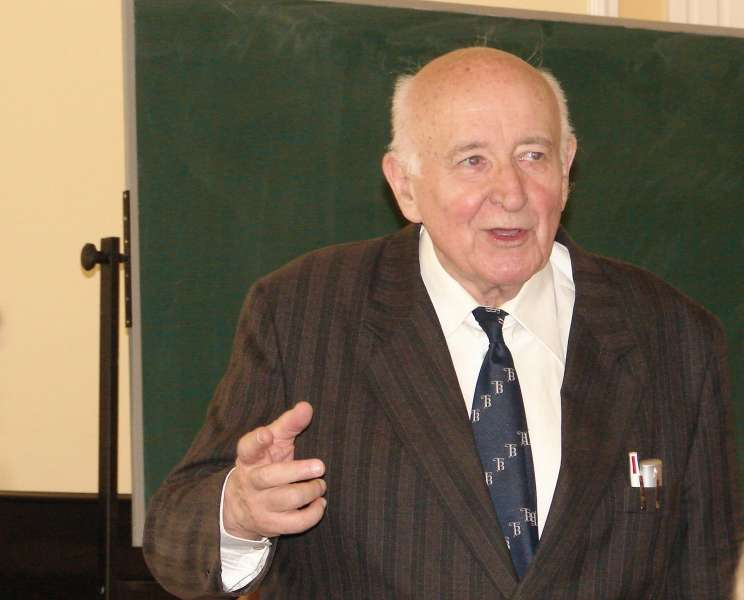
\includegraphics[height=\the\HauteurDesPhotos]{Kurzweil}&
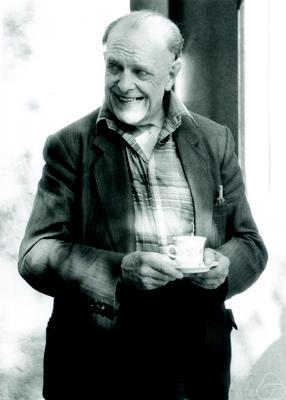
\includegraphics[height=\the\HauteurDesPhotos]{Henstock}\\
Kurzweil&Henstock%
\end{tabular}}
\medskip
\ImageAGauche{%
\textcolorgris{Dans les années 50 a été mise au point l'intégrale de Kurzweil-Henstock\index[aut]{Kurzweil (Jaroslav), 1926-, Tchèque}\index[aut]{Henstock (Ralph), 1923-2007, Anglais} (ou KH-intégrale, ou intégrale de jauge) à partir de celle de Riemann. On retravaille un peu les sous-intervalles et les points de calcul de la fonction: chaque point est appelé «marque» et l'on parle de «subdivision marquée» (pour plus de détails, chercher «lemme de Cousin». Pierre Cousin\index[aut]{Cousin (Pierre), 1867-1933, Français} était un étudiant de Henri Poincaré).\index[aut]{Poincaré (Henri), 1854-1912, Français}\\ 
\indent Sans faire appel à la théorie de la mesure, on dispose alors d'une intégrale aussi puissance que celle de Lebesgue (mais moins générale, car définie uniquement sur~$\RR$). Et on dispose même d'un très beau résultat: toute fonction dérivée est intégrable, et il n'est pas nécessaire d'introduire la notion d'intégrale impropre. L'intégrale de Lebesgue peut alors être introduite comme un cas particulier de cette intégrale.}}
\end{histoire}\colorblack




\medskip
\section{Présentation des espaces de Lebesgue~$L^p$}\index{espace!de Lebesgue}\index[aut]{Lebesgue (Henri-Léon), 1875-1941, Français}

\begin{definition}[Ensemble des fonctions mesurables]
Soit~$(E,\mathcal{A},\mu)$ un espace mesuré.
Si~$\colorred p\in\intfo{1}{+\infty}$, on note~$\colorblue \mathcal{L}^p=\mathcal{L}^p(E,\mathcal{A},\mu)$ l'ensemble de toutes
les fonctions mesurables sur~$(E,\mathcal{A})$, à valeurs dans~$\RR$, telles que la fonction
$|f|^p$ soit~$\mu$-intégrable.

Si~$f\in\mathcal{L}^p$, on pose:
\begin{equation}\|f\|_p=\left(|f|^p\dd\mu\right)^{1/p} \end{equation}
\end{definition}

\begin{theoreme}
Chaque espace~$\mathcal{L}^p$ est un espace vectoriel.
\end{theoreme}

\begin{definition}[Espace~$L^p$]
Soit~$(E,\mathcal{A},\mu)$ un espace mesuré.
Si~$\colorred p\in\intfo{1}{+\infty}$, on note~$\colorblue L^p=L^p(E,\mathcal{A},\mu)$ l'ensemble des
classes d'équivalence des fonctions de~$\mathcal{L}^p$ pour la relation d'équivalence
«égualité~$\mu$-presque partout».

Si~$f\in L^p$, on note~$\|f\|_p$ la valeur commune des~$\| g\| _p$ pour toutes les fonctions~$g$
appartenant à la classe de~$f$.
\end{definition}

De manière équivalente, on peut également définir~$L^p$ comme étant le quotient de~$\mathcal{L}^p$ par la relation d'équivalence «égalité~$\mu$-presque partout».
%%%%%%%%%%%%%%%%%%%%%%%%%%%%
\medskipvm
Il est clair que chaque espace~$L^p$ est une classe d'équivalence obtenu en identifiant les fonctions qui ne diffèrent que sur un ensemble négligeable. Ainsi, si~$f\in L^p$, on appelle «représentant» de~$f$, toute fonction mesurable~$g\in\mathcal{L}^p$ qui appartient à la classe d'équivalence de~$f$.

Comme, par construction, deux représentant d'une même classe auront la même intégrale, on
appelle (abusivement, mais sans confusion) tout~$f\in L^p$ une fonction de~$L^p$ et non pas une classe d'équivalence ou un représentant de la classe d'équivalence.
En d'autres termes, on identifie une classe à l'un quelconque de ses représentants.

\medskip
\textcolorgris{En toute généralité, on aura bien remarqué que les définitions précédentes sont liées à la mesure~$\mu$ utilisée. Si l'on considère simultanément deux mesures~$\mu$ et~$\nu$, les classes d'équivalences ne sont pas les mêmes respectivement à chacune de ces mesures, et l'identification d'une classe à l'un quelconque de ses représentant ne peut plus se faire.}

\begin{theoreme}
Chaque espace~$L^p$ est un espace vectoriel.
\end{theoreme}

Un espace~$L^p$ est un espace vectoriel (des classes) de fonctions dont la puissance d'exposant~$p$ est
intégrable au sens de Lebesgue, où~$p$ est un nombre réel strictement positif.
Le passage à la limite de l'exposant aboutit à la construction des espaces~$L^\infty$ des fonctions
bornées.

\medskip
\begin{theoreme}
Chaque espace~$L^p$ est un espace de Banach lorsque son exposant~$p$ est~$\ge 1$.
\end{theoreme}

\begin{theoreme}
Lorsque~$0 < p < 1$, l'intégrale définit une quasi-norme qui en fait un espace complet.
\end{theoreme}


\medskip
\begin{definition}[Exposants conjugués]\index{exposant conjugué!de Lebesgue}
Soient~$p$ et~$q\in [1,+\infty]$. On dit que~$p$ et~$q$ sont des exposants conjugués si:
\begin{equation}\colorred\dfrac1p + \dfrac1q = 1 \end{equation}
\end{definition}

\begin{theoreme}
Soient~$p$ et~$q$ des exposants conjugués, alors il existe une \textcolorblue{dualité} entre les espaces d'exposants~$p$ et~$q$.
\end{theoreme}
\colorgris
Il suffit en effet de considérer, à~$g\in L^q$ fixé (de mesure~$\mu$), l'application~$\varphi_g: f\mapsto \int fg\dd\mu$. Cette dernière
définie une forme linéaire continue sur~$L^p$.
\colorblack

\medskip
\section{Construction de~$L^p$}

On considère~$\Omega$ un ouvert de~$\RR^n$.
Les fonctions~$f$ seront considérées de~$\Omega$ dans~$\RR$ ou~$\CC$.

\medskip
On appelle~$\colorblue L^p \colorblack= L^p_M(\Omega,\CC)$ pour~$p<\infty$ l'espace des fonctions~$f$ mesurables, de~$\Omega \rightarrow \CC$, telles que $\mu(|f|^p)<\infty$ où~$\mu$ est une mesure sur~$\Omega$.

\medskip
Comme une fonction s'annulant presque partout est d'intégrale nulle, on peut définir l'espace~$L^p(X, \mathcal{A}, \mu)$ comme le quotient de l'espace des fonctions~$p$ intégrables $L^p(X, \mathcal{A}, \mu)$ par le sous-espace vectoriel des fonctions presque nulles.

\textcolorgreen{Ce quotient identifie donc les fonctions qui sont presque partout égales, autrement dit qui ne diffèrent que sur un ensemble de mesure nulle.}

\medskip
\begin{definition}[Norme~$L^p$]
Pour~$p<\infty$, on appelle \textcolorblue{norme~$L^p$} et on note~$\|\cdot\|_p$, l'application définie par:
\begin{equation}\|f\|_p=\left(\dint_\Omega |f|^p\right)^{1/p}
\end{equation}
\end{definition}
\begin{itemize}
\item Sur~$\RR$, cela donne:
\begin{equation}\|f\|_p=\left(\dint_a^b |f(t)|^p\dd t\right)^{1/p}\end{equation}
\item Sur un espace mesuré~$(X, \mathcal{A}, \mu)$ et à valeurs réelles ou complexes:
\begin{equation}\|f\|_p=\left(\dint_X |f|^p\dd\mu\right)^{1/p}\end{equation}
\end{itemize}
\medskip
\begin{theoreme}
Si l'espace~$X$ est fini et est muni d'une mesure finie~$\mu(X)<\infty$, alors tous les espaces~$L^p$ (resp.~$\mathcal{L}^p$), pour~$1\le p\le \infty$ sont les mêmes.
\end{theoreme}

\begin{definition}[Espace des suites]
Soit~$X=\NN$ muni de sa tribu~$\mathcal{A}=\mathcal{P}(X)$ et de sa mesure de comptage~$\mu$.
On note~$\ell^p$ l'espace~$L^P(X,\mathcal{A},\mu)=\mathcal{L}^p(X,\mathcal{A},\mu)$.
Cet espace est l'espace des suites~$(u_n)_{n\in\NN}$ telles que:
\begin{equation}
\left\{
\begin{array}{lll}
\text{Si } 1\le p<\infty: &\quad \dsum_n |u_n|^p<\infty, &\quad \text{ et } \|u_n\|_p=\left(\dsum_n|u_n|^p\right)^{1/p}\\
\text{Si } p=\infty: &\quad \sup_n |u_n|^p<\infty, &\quad \text{ et } \|u_n\|_\infty=\sup_n|u_n|
\end{array}
\right.
\end{equation}
\end{definition}

\medskip
\section{Espace~$L^0$}
L'espace~$L^0$ est l'ensemble des fonctions mesurables.
$L^0$ est l'espace obtenu en quotientant~$\mathcal{L^0}$ par les fonctions nulles.

\medskip
Soit~$\varphi$ une fonction mesurable strictement positive et~$\mu$-intégrable, alors:
\begin{equation}
\rho(f,g)=\dint \frac{\|f-g\|}{1+\|f-g\|} \varphi \dd\mu
\end{equation}
définit une distance sur~$L^0$ qui redonne la topologie de la convergence en mesure.

\begin{theoreme}
Muni de cette distance, l'espace~$L^0$ est complet.
\end{theoreme}

\medskip
Rappel: la notion de convergence (de suite) est une propriété topologique et non métrique (l'écriture avec les~$\varepsilon$ n'est que la traduction métrique de l'écriture topologique avec les boules).

\medskip
\section{Espace~$L^\infty$ et dualité avec~$L^1$}
Dans le cas où l'exposant est infini, on procède de la même manière.

\medskip
L'espace~$L^\infty(X, \mathcal{A}, \mu)$ est défini comme l'espace vectoriel des fonctions $\mu$-essentiellement bornées (i.e. des fonctions bornées presque partout).

L'espace~$L^\infty(X, \mathcal{A}, \mu)$ est l'espace vectoriel quotient de~$L^\infty(X, \mathcal{A}, \mu)$
par la relation d'équivalence «$f \sim g$» ssi «$f$ et~$g$ sont égales presque partout».

\begin{theoreme}
L'espace dual de~$L^1$ est~$L^{\infty}$ mais l'espace dual de~$L^{\infty}$ contient strictement~$L^1$.
\end{theoreme}

\medskip
\section{Espace~$L^2$}

Par définition, si~$\Omega$ est un ouvert donné de~$\RR^n$, $L^2(\Omega)$ est l'espace des fonctions (réelles ou complexes) qui sont de carré intégrable au sens de l'intégrale de Lebesgue.

\medskip
\begin{theoreme}
\textcolorred{L'espace~$L^2$ est un espace de Hilbert lorsqu'il est muni du produit scalaire:
\begin{equation}(f,g) = \dint_{\Omega} f \bar g \,\dd\mu\end{equation}}\index{produit scalaire!de~$L^2$}
\end{theoreme}

\medskip
La formule des exposants conjugués conduit dans le cas~$p=2$, à~$q=2$, i.e. que \textcolorred{$L^2$ s'identifie à son dual.}

\textcolorgris{Si l'on reprend la remarque précédente sur la dualité, cela devient dans~$L^2$ (et dans tout espace de Hilbert~$H$): en associant à tout~$v\in H$ l'application~$\varphi_v(u)=\langle u,v\rangle$, on peut identifier l'espace de Hilbert~$H$ a son dual~$H'$.}

\medskip
\textcolorgreen{Comme mentionné, l'intérêt d'avoir un espace de Hilbert est de disposer d'un produit scalaire, donc de pouvoir décomposer un vecteur. Ce que l'on retrouve dans le théorème \ref{th:projHilbert}, que nous réécrivons ci-dessous, et vrai dans~$L^2$ en tant qu'espace de Hilbert:}

\begin{theoreme}[Théorème de projection dans un espace de Hilbert]\index{théorème!de projection (dans un Hilbert)}
Tout vecteur~$u$ d'un espace de Hilbert~$H$ se décompose de manière unique en une somme~$u=v+w$ avec $v\in K$ et~$w\in K^\bot$, et les sous-espaces~$K$ et~$K^\bot$ sont supplémentaires dans~$H$.
\end{theoreme}

On rappelle que:
\begin{definition}[Orthogonal d'une partie]
$K$ étant une partie de~$H$, on note~$K^\bot$ l'ensemble des vecteurs~$u\in H$ qui sont orthogonaux à tous les
vecteurs de~$K$.
\end{definition}

\begin{theoreme}
L'orthogonal~$K^\bot$ de toute partie de~$K$ d'un espace de Hilbert~$H$ est un sous-espace vectoriel fermé de $H$, donc lui-même un espace de Hilbert (théorème \ref{Th-SsH}).

On a~$(K^\bot)^\bot = K$.
\end{theoreme}

\medskip
\section{Compléments}

Commençons par quelques exemples ultra classiques:
\begin{itemize}
  \item La fonction~$1/\sqrt{x}$ est~$L^1$ mais pas~$L^2$.
  \item La fonction~$1/|x|$ est~$L^2$ mais pas~$L^1$.
  \item La fonction~$\mathrm{e}^{-|x|}/\sqrt{|x|}$ est~$L^1$ mais pas~$L^2$
\end{itemize}

\medskip
Poursuivons par quelques inégalités bien utiles.

\begin{theoreme}[Inégalité de Minkowski]\index[aut]{Minkowski (Hermann), 1864-1909, Allemand}
Soient~$p\in[1,\infty]$, et~$f$ et~$g$ dans~$L^p$, alors on a:
\begin{equation}\|f+g\|_p\le\|f\|_p+\|g\|_p\end{equation}
\end{theoreme}

\begin{theoreme}[Inégalité de Hölder]\index[aut]{Hoelder@Hölder (Otto Ludwig), 1859-1937, Allemand}
Soient~$p$, $q$ et~$r$ des nombres de~$[1,\infty]$ vérifiant;
\begin{equation}\dfrac1p+\dfrac1q=\dfrac1r\end{equation} (avec la convention~$1/\infty=0$).
Si~$f\in L^p$ et~$g\in L^q$, alors le produit~$fg\in L^r$, et on a:
\begin{equation}\|fg\|_r\le\|f\|_p\|g\|_q\end{equation}
\end{theoreme}

L'inégalité de Hölder conduit au théorème suivant:
\begin{theoreme}
Si~$\mu$ est une mesure finie et si~$1\le p\le q\le \infty$, on a:
\begin{equation}L^q\subset L^p\end{equation}
\end{theoreme}

\medskip
Terminons en revenons un peu à nos fonctions continues~$C^k$, et plus précisément sur les fonctions continues à support compact
dans un ouvert~$\Omega$ mesurable de~$\RR^n$ (voir la définition~\ref{Def-Cc} page \pageref{Def-Cc}).
On dispose des résultats de \textcolorblue{densité} suivants:
\begin{itemize}
  \item L'espace~$C_c^0(\Omega)$ des fonctions continues à support compact est dense dans~$L^p(\Omega)$ pour~$1\le p<\infty$
	(mais n'est pas dense dans~$L^\infty(\Omega)$)

	\colorgris Dans le cas~$p=1$, cela se traduit par: 	$ \forall f\in L^1(\Omega), \forall\varepsilon>0, \exists g\in C_ c^0(\Omega), \text{ tel que }
	  \|f-g\|_{L^1(\Omega)}\le\varepsilon$ \colorblack

  \item L'espace~$C_c^\infty(\Omega)$ des fonctions infiniment dérivables à support compact est dense dans~$L^p(\Omega)$ pour~$1\le p<\infty$
	(mais n'est pas dense dans~$L^\infty(\Omega)$)
  \item L'espace~$C_c^\infty(\Omega)$ est dense dans le sous espace de~$L^\infty(\Omega)$ des fonctions bornées qui tendent vers 0 en l'infini.
  \item L'ensemble des fonctions continues à support compact de~$L^p(\RR^n)$ est dense dans~$L^p(\RR^n)$, pour~$p\neq\infty$. 
\end{itemize}

\textcolorgreen{Les arguments de densité ont une importance pratique dans certaines démonstrations:}
si l'on doit démontrer qu'une propriété est vérifiée sur~$L^p(\Omega)$, alors on peut commencer par montrer que cette propriété est vraie sur~$C_c^\infty(\Omega)$, avant de passer à la limite en utilisant l'argument de densité: «$C_c^\infty(\Omega)$ est dense dans~$L^p(\Omega)$».

\medskip
L'espace~$C_c^{\infty}(\Omega)$ est également noté~$\mathcal{D}(\Omega)$ et appelé espace des fonctions tests. 
Les distributions sont définies comme les éléments de~$\mathcal{D}'(\Omega)$, dual topologique de~$\mathcal{D}(\Omega)$, muni d'une topologie adéquate.
Nous allons les aborder dès a présent, au chapitre~\ref{Ch-Sobo}.

% \chapter{Espaces de Sobolev}\label{Ch-Sobo}\index[aut]{Sobolev (Sergueï Lvovitch), 1908-1989, Russe}
\begin{abstract}
Les espaces de Sobolev sont des espaces fonctionnels.
Plus précisément, un espace de Sobolev est un espace vectoriel de fonctions muni de la norme obtenue par la combinaison de la norme~$L^p$ de la fonction elle-même ainsi que de ses dérivées jusqu'à un certain ordre.
Les dérivées sont comprises dans un sens faible, au sens des distributions afin de rendre l'espace complet.

Les espaces de Sobolev sont donc des espaces de Banach.
Intuitivement, un espace de Sobolev est un espace de Banach ou un espace de Hilbert de fonctions pouvant être dérivées suffisamment de fois (pour donner sens par exemple à une équation aux dérivées partielles) et muni d'une norme qui mesure à la fois la taille et la régularité de la fonction.

Les espaces de Sobolev sont un outil très important et très adapté à l'étude des équations aux dérivées partielles. En effet, les solutions d'équations aux dérivées partielles, appartiennent plus naturellement à un espace de Sobolev qu'à un espace de fonctions continues dont les dérivées sont comprises dans un sens classique (mais rien n'empêche d'avoir de la chance).
\end{abstract}

\medskip
\begin{histoire}%
Le \textsc{xx}\fup{e} siècle avait commencé par la thèse de Lebesgue\index[aut]{Lebesgue (Henri-Léon), 1875-1941, Français} \emph{intégrale, longueur, aire}, qui constitue vraiment le début de la théorie de la mesure.
La théorie de Lebesgue mène à l'étude des espaces~$L^p$, qui permettront, sur les traces de Hilbert,\index[aut]{Hilbert (David), 1862-1943, Allemand} Riesz\index[aut]{Riesz (Frigyes), 1880-1956, Hongrois} et Banach,\index[aut]{Banach (Stephan), 1892-1945, Polonais} l'étude des opérateurs différentiels.

\sbox{\MaBoiteAvecPhotos}{\setlength{\tabcolsep}{0pt}\scriptsize%
\begin{tabular}{cccc}
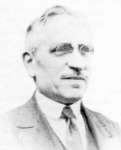
\includegraphics[height=\the\HauteurDesPhotos]{Lebesgue3}&
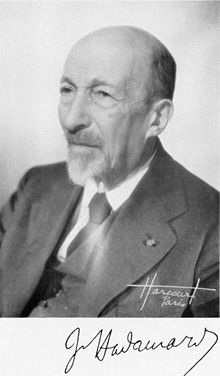
\includegraphics[height=\the\HauteurDesPhotos]{Hadamard}&
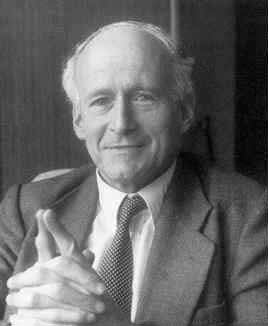
\includegraphics[height=\the\HauteurDesPhotos]{Schwartz}&
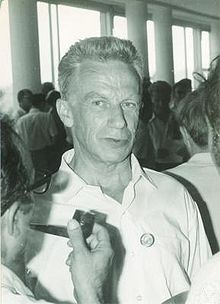
\includegraphics[height=\the\HauteurDesPhotos]{Sobolev}\\
Lebesgue &Hadamard &Schwartz &Sobolev%
\end{tabular}}
\medskip
\ImageADroite{%\ifVersionDuDocEstVincent\begin{cutout}{0}{0.50\linewidth}{0pt}{8}\else\begin{cutout}{0}{0.44\linewidth}{0pt}{8}\fi
Cauchy\index[aut]{Cauchy (Augustin Louis, baron -), 1789-1857, Français} avait publié nombre d'applications de sa théorie dans des recueils d'exercices, notamment concernant l'évaluation d'intégrales réelles, qu'il n'hésita pas à généraliser en ce qu'on appelle aujourd'hui la «valeur principale de Cauchy», un peu moins d'un siècle avant que Hadamard\index[aut]{Hadamard (Jacques Salomon), 1865-1963, Français} en ait besoin dans sa résolution des équations aux dérivées partielles dans un problème d'hydrodynamique par les «parties finies» et que Laurent Schwartz\index[aut]{Schwartz (Laurent), 1915-2002, Français} n'en vienne aux distributions.}

\medskip
L'étude des conditions de régularité des solutions des équations aux dérivées partielles permet à Sergueï Sobolev\index[aut]{Sobolev (Sergueï Lvovitch), 1908-1989, Russe} et ses continuateurs de définir ses espaces de fonctions et les théorèmes de trace en fonction des propriétés géométriques du domaine.

\medskip
Quelques mots s'imposent au sujet de la théorie des distributions.
Parmi tous les travaux ayant valus à leur auteur la médaille Fields, la théorie des distributions de Laurent Schwartz\index[aut]{Schwartz (Laurent), 1915-2002, Français} est l'une des très rares à être abordable par les étudiants dès leur premier cycle universitaire. C'est une partie de l'explication du réel engouement pour les distributions, l'autre partie étant sa puissance, sa commodité d'usage et surtout sa très grande beauté.

Si cette théorie fournit aux analystes un cadre général et un formalisme agréable pour l'étude des espaces fonctionnels et des équations aux dérivées partielles dans lesquels ils aiment à se placer, elle n'est pourtant pas indispensable.
D'une part, les spécialistes d'équations aux dérivées partielles parviennent toujours à trouver des formulations bien adaptées à leurs problèmes, en s'inspirant des idées sous-jacentes à la théorie des distributions, mais sans y avoir recours explicitement. D'autre part, on peut étudier la plupart des espaces fonctionnels intéressants sans la notion de distribution: par exemple, les espaces de Sobolev peuvent être définis en termes de  distributions, ou bien en termes de complétion de l'espace des fonctions $C^\infty$ à support compact pour des normes bien choisies. %L'équivalence de ces deux points de vue est d'ailleurs un résultat célèbre dû à Meyers et Serin.

En utilisant uniquement des espaces de Sobolev et leurs espaces duals, on peut obtenir la grande majorité des distributions que l'on rencontre en pratique: par exemple, la dérivée de la «fonction de Dirac»\index[aut]{Dirac (Paul Adrien Maurice), 1902-1984, Anglais} peut être vue comme un élément de l'espace dual des fonctions $C^1$. Plus généralement, quand on rencontre une distribution dans un problème concret, c'est presque à coup sûr un élément du dual d'un espace de Sobolev bien choisi, au moins localement. La topologie des espaces de Sobolev étant beaucoup plus simple que celle des distributions, on comprend que l'étude des espaces de Sobolev soit plus populaire et certainement plus utile en pratique. De plus, les résultats que l'on obtient en utilisant des méthodes plus terre-à-terre sont souvent meilleurs (plus constructifs, plus quantitatifs...).

Pour autant, la théorie des distributions fournit un formalisme commode et élégant, qui apporte de l'ordre dans le paysage fonctionnel, et facilite la communication entre mathématiciens d'horizons très divers. En outre, les principes qui la sous-tendent, bien plus que les théorèmes principaux, s'avèrent d'une importance capitale en pratique. Pour toutes ces raisons, une bonne familiarité avec le langage des distributions est presque indispensable à un analyste. Schwartz\index[aut]{Schwartz (Laurent), 1915-2002, Français} lui-même avait bien conscience que le principal mérite de son approche ne résidait pas dans l'introduction d'outils nouveaux, mais dans une synthèse claire et accessible de recettes multiples qui étaient, déjà auparavant, employées dans des contextes divers.
\end{histoire}
\colorblack

\medskip
\section{Distributions}\index{distribution}
Une distribution (également appelée fonction généralisée) est un objet qui généralise la notion de fonction et de mesure. La théorie des distributions étend la notion de dérivée à toutes les fonctions localement intégrables et au-delà.

\begin{histoire}
\noindent\emph{Généralisation de la notion de fonction:}\\
\sbox{\MaBoiteAvecPhotos}{\setlength{\tabcolsep}{0pt}\scriptsize%
\begin{tabular}{c}
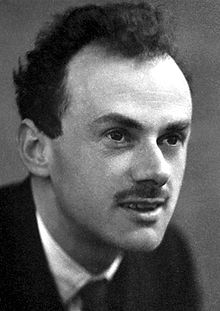
\includegraphics[height=\the\HauteurDesPhotos]{Dirac}\\
Dirac%
\end{tabular}}
\ImageADroite{%
Depuis le milieu des années 1920, les théoriciens de la physique quantique, et en particulier Dirac,\index[aut]{Dirac (Paul Adrien Maurice), 1902-1984, Anglais} utilisaient des objets étranges qu'ils manipulaient comme des fonctions. Le plus typique était la «fonction de Dirac»,\index[aut]{Dirac (Paul Adrien Maurice), 1902-1984, Anglais} mystérieuse fonction qui vaut $0$ partout, sauf en $0$ où elle vaut $+\infty$, et dont l'intégrale est égale à $1$ (en violation de toutes les règles de la théorie de l'intégration de Lebesgue). Non seulement Dirac\index[aut]{Dirac (Paul Adrien Maurice), 1902-1984, Anglais} utilisait cette fonction à des fins de calcul formel, mais encore il se permettait de la dériver à volonté, se contentant de remarquer que les dérivées successives étaient «de plus en plus singulières».\\
\indent L'utilité et le caractère intuitif de ces objets rendait presque indispensable leur incorporation dans une théorie mathématique; c'est ce qu'a réalisé la théorie des distributions. Leur interprétation est d'ailleurs très simple, et cause beaucoup moins de
maux de tête que les interrogations que l'on peut avoir sur la nature des «fonctions»
considérées par Dirac.\index[aut]{Dirac (Paul Adrien Maurice), 1902-1984, Anglais}}

\medskip
\noindent\emph{Réhabilitation de la dérivation:}\\
\sbox{\MaBoiteAvecPhotos}{\setlength{\tabcolsep}{0pt}\scriptsize%
\begin{tabular}{cc}
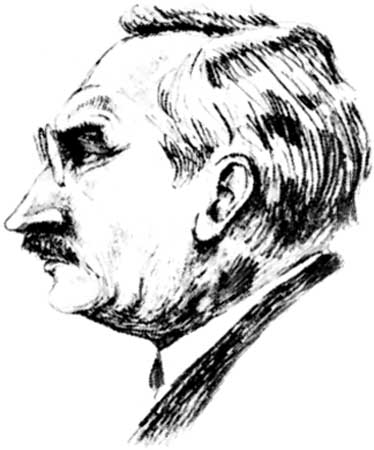
\includegraphics[height=\the\HauteurDesPhotos]{Lebesgue4}&
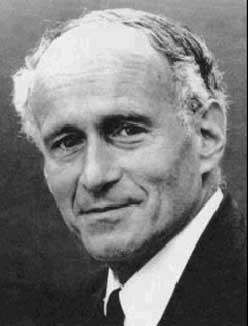
\includegraphics[height=\the\HauteurDesPhotos]{Schwartz2}\\
Lebesgue&Schwartz%
\end{tabular}}
\ImageAGauche{%
Au début du vingtième siècle, la théorie de l'intégration de Lebesgue a pris un essor rapide, et l'intégration apparaît désormais comme l'opération reine de l'analyse. La plupart des fonctions sont intégrables, alors que très peu sont dérivables. En outre, la théorie de Lebesgue montre que l'intégration est souvent une opération continue vis-à-vis de la convergence des fonctions, uniforme ou même simple (ponctuelle), alors que la dérivation est une opération grossièrement discontinue.\\
\indent
Dans la théorie de Schwartz\index[aut]{Schwartz (Laurent), 1915-2002, Français} au contraire, ces problèmes disparaîtront: à toute fonction continue on pourra associer des «fonctions dérivées» à tous les ordres, selon une notion qui prolongera celle de dérivée des fonctions continûment dérivables. De manière plus générale, toute distribution sera dérivable à tout ordre, et on pourra définir une notion de convergence qui prolongera la notion de convergence uniforme, et pour laquelle l'opération de dérivée sera continue.}

\medskip
\noindent\emph{Extension des espaces de solutions acceptables:}\\[+2.5mm]
Leray\index[aut]{Leray (Jean), 1906-1998, Français} en 1934 et Sobolev\index[aut]{Sobolev (Sergueï Lvovitch), 1908-1989, Russe} en 1936 introduisent de nouvelles notions de solutions d'équations aux dérivées partielles, appelées solutions faibles ou solutions généralisées, qui permettent de formuler des équations aux dérivées partielles sans supposer nécessairement l'existence de dérivées au sens classique. Leur approche préfigure très bien la théorie des distributions, qui ne sera mise au point qu'une quinzaine d'années plus tard. Les contributions de Leray et Sobolev ne constituent pas les seuls travaux précurseurs de la théorie des distributions. Dans les années 30 et 40, de nombreux chercheurs vont utiliser les concepts de solutions généralisées pour étudier les solutions de diverses équations aux dérivées partielles: Courant\index[aut]{Courant (Richard), 1888-1972, Américain} et Hilbert,\index[aut]{Hilbert (David), 1862-1943, Allemand} Bochner,\index[aut]{Bochner (Salomon), 1899-1982, Américain} Friedrichs,\index[aut]{Friedrichs (Kurt Otto), 1901-1982, Allemand} Krylov...\index[aut]{Krylov (Aleksey Nikolaevich), 1863-1945, Russe}

\sbox{\MaBoiteAvecPhotos}{\setlength{\tabcolsep}{0pt}\scriptsize%
\begin{tabular}{cc}
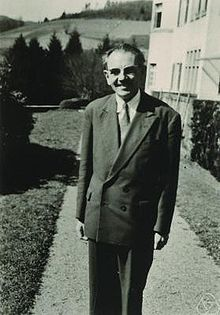
\includegraphics[height=\the\HauteurDesPhotos]{Leray}&
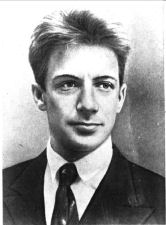
\includegraphics[height=\the\HauteurDesPhotos]{Sobolev2}\\
Leray&Sobolev%
\end{tabular}}
\ImageADroite{%
Nous arrivons maintenant à l'idée majeure de la théorie des distributions, déjà présente dans les travaux de Sobolev\index[aut]{Sobolev (Sergueï Lvovitch), 1908-1989, Russe} et Leray.\index[aut]{Leray (Jean), 1906-1998, Français} Du point de vue physique, on peut la motiver comme suit. Le résultat ou l'interprétation d'une expérience physique faisant intervenir une certaine grandeur, qui varie en fonction du temps ou de l'espace, ne dépend que très rarement des valeurs ponctuelles de cette grandeur, mais plus souvent de sa valeur moyenne (ou intégrale) prise contre une fonction du temps ou de l'espace, plus ou moins localisée. En d'autres termes, plutôt qu'une fonction $u$, c'est plutôt une «moyenne» de la forme $\int u\varphi$ qui sera accessible en pratique. Ainsi, un signal électrique oscillant avec une période très élevée fournira, de manière apparemment paradoxale, un signal plat quand on l'utilisera pour alimenter un oscilloscope: dans le processus de moyenne inhérent à la mesure, les valeurs positives et négatives se compenseront.}

Dans le cas de l'équation des ondes aussi bien que dans celui des équations de transport avec données singulières, on résout ainsi le dilemme qui nous est proposé, en reformulant l'équation par son action sur les fonctions-test.

Explicitons plus en détail la réflexion de Sobolev.\index[aut]{Sobolev (Sergueï Lvovitch), 1908-1989, Russe} Pour des raisons ayant trait
à l'analyse (fonctionnelle) de certaines classes d'équations aux dérivées partielles,
il cherchait à étudier les fonctions possédant une dérivée carré-intégrable, dans un
cadre suffisamment général... et en particulier, sans supposer la fonction dérivable!
Il montra que l'on pouvait donner une définition utile et pratique du concept de «fonction dont la dérivée est de carré intégrable», qui ne présuppose pas l'existence d'une dérivée au sens usuel. L'espace ainsi défini est aujourd'hui appelé espace de Sobolev $W^{1,2}$ ou $H^1$.

\medskip
\noindent\emph{Simplification de problèmes non linéaires ardus:}\\[+2.5mm]
L'utilisation de solutions généralisées peut venir d'une nécessité de modélisation, mais également par l'incapacité à prouver l'existence de solutions classiques. L'exemple archétypal en la matière est celui des équations de la mécanique des fluides, en particulier l'équation de Navier-Stokes\index[aut]{Navier (Claude Louis Marie Henri), 1785-1836, Français}\index[aut]{Stokes (George Gabriel), 1819-1903, Anglais} incompressible, dont la première étude mathématique moderne est due à Leray.\index[aut]{Leray (Jean), 1906-1998, Français} L'écriture même de l'équation de Navier-Stokes incompressible présuppose apparemment la dérivabilité de la fonction inconnue $u$, mais rien ne semblait permettre d'affirmer l'existence de solutions dérivables pour des données initiales assez générales. Ce problème est d'ailleurs toujours ouvert, et compte parmi les sept problèmes du millénaire de l'Institut Clay, mais nous en reparlerons au paragraphe~\ref{Sec-NavierStokes}. Leray\index[aut]{Leray (Jean), 1906-1998, Français} eut l'idée de définir une solution de l'équation de Navier-Stokes incompressible par une formulation duale qui ne présupposait pas de régularité. De telles solutions sont aujourd'hui appelées solutions faibles.

\medskip
La théorie des distributions exploite au maximum l'idée de moyenner les solutions contre des fonctions-test qui se comportent bien: on définit au départ une classe agréable de fonctions-test, à la fois très régulières et bien localisées, à savoir les fonctions indéfiniment dérivables, à support compact. Toutes les propriétés des objets que l'on cherche à définir sont alors définies en fonction des «intégrales» de ces objets contre les fonctions-test.
\end{histoire}

\medskip
\begin{definition}[Espace des fonctions tests~$\mathcal{D}(\Omega)$]
Soit~$\Omega$ un sous-espace topologique de~$\RR^n$ (ou~$\CC^n$).
\textcolorblue{L'espace des fonctions tests~$\mathcal{D}(\Omega)$} est l'ensemble des fonctions à valeurs réelles indéfiniment dérivables de~$\Omega$ à support compact inclus dans~$\Omega$.

On munit cet espace vectoriel de la topologie suivante: un ensemble~$U \subset \mathcal{D}(\Omega)$ est ouvert si et seulement si~$\forall K \subset \Omega$ compact et~$f \in U$ dont le support est inclus dans~$K$, il existe~$\epsilon > 0$ et~$k \ge 0$ tels que:
\begin{equation}
  \{ g \in \mathcal{D}(\Omega)\;\mid\; \operatorname{supp}(g) \subset K\quad\text{ et }\quad\forall x \in K,\; |f^{(k)}(x)-g^{(k)}(x)|\le \epsilon \}\;\subset\;U.
\end{equation}
Muni de cette topologie, $\mathcal{D}(\Omega)$ est un espace vectoriel topologique \textcolorred{non métrisable}.
\end{definition}

\medskip
\begin{definition}[Distribution]
\textcolorblue{Une distribution} est une \textbf{forme linéaire continue}\index{forme!linéaire} sur~$\mathcal{D}(\Omega)$.
\end{definition}

L'ensemble des distributions est donc le dual topologique de~$\mathcal{D}(\Omega)$ et est par conséquent noté~$\mathcal{D}'(\Omega)$.\index{dual topologique d'un espace vectoriel}

\begin{remarque}
L'espace des distributions est extrêmement grand, et contient tous les espaces fonctionnels que nous avons mentionnés jusqu'à présent et leur dual, y compris les espaces à poids et les espaces locaux (non présentés dans ce document).
\end{remarque}\colorgris
\begin{remarque}[Complément topologique]
L'espace~$\mathcal{D}$ n'est pas métrisable. Définir sa topologie n'est pas équivalent à définir la convergence des suites. Cependant, dans la pratique c'est presque la seule notion de convergence que l'on utilise.

\medskip
Soit~$\Omega$ un ouvert de~$\RR^n$. On muni~$\mathcal{D}'(\Omega)$ de la topologie faible-* induite par~$\mathcal{D}(\Omega)$. Alors:\\
-- $\mathcal{D}'(\Omega)$ est un espace topologique complet (et un espace de Montel);\index[aut]{Montel (Paul Antoine Aristide Montel), 1876-1975, Français}\\
-- Le dual topologique de~$\mathcal{D}'(\Omega)$ s'identifie à~$\mathcal{D}(\Omega)$, qui est donc réflexif;\\
-- La topologie de~$\mathcal{D}'(\Omega)$ n'est pas métrisable.

\medskip
Notons que la convergence dans le dual de n'importe quel espace de Sobolev implique la convergence au sens des distributions.
\end{remarque}\colorblack

Toujours aussi classiquement, si~$T$ est une distribution et~$\varphi$ une fonction test de $\mathcal{D}(\Omega)$ alors on note~$T(\varphi)=\langle T,\varphi \rangle$. (où~$\langle\cdot,\cdot\rangle$ désigne comme d'habitude le crochet de dualité).
\medskipvm
Dans~$\mathcal{D}'(\mathbb{R})$, l'application qui à~$\varphi$ associe~$\varphi(0)$ est une distribution et c'est la distribution de Dirac\index{distribution!de Dirac}\index[aut]{Dirac (Paul Adrien Maurice), 1902-1984, Anglais}:
\begin{equation}
\langle\delta,\varphi\rangle=\varphi(0)
\end{equation}
\medskipvm
Une propriété fondamentales est que \textcolorblue{toute fonction localement intégrable~$f$ représente aussi une distribution~$T_f$ définie par la forme intégrale suivante}:
\begin{equation}
  \langle T_f,\varphi\rangle=\int_{\mathbb{R}}f(x)\varphi(x)\,\dd x, \quad \forall \varphi\in\mathcal{D}(\Omega)
\end{equation}


\medskip
\section{Dérivées au sens des distributions}\index{dérivée!au sens des distributions}
Pour définir la dérivée d'une distribution, considérons d'abord le cas d'une fonction différentiable et intégrable~$f:\mathbb{R}\rightarrow\mathbb{R}$.
Soit~$\varphi$ une fonction test, supposée régulière et à support compact.
Une intégration par parties permet d'écrire:
\begin{equation}
  \int_\RR f'(x) \varphi(x)\,\dd x = -\int_\RR f(x)\varphi'(x)\,\dd x \qquad\text{ soit }\qquad I_{f'}(\varphi)=I_{-f}(\varphi')
\end{equation}
En effet, puisque la fonction~$\varphi$ est nulle en dehors d'un ensemble borné (elle est à support compact), les termes de bords s'annulent.

\medskip
\begin{definition}[Dérivée d'une distribution]\label{Def-DerivDistrib}
Si~$S$ est une distribution, cet exemple suggère que l'on puisse \textcolorblue{définir sa dérivée~$S'$ comme la forme linéaire} qui à une fonction test~$\varphi$ fait correspondre la valeur~$- S(\varphi')$. On pose donc:
\begin{equation}\colorred
  \langle S', \varphi \rangle = - \langle S, \varphi' \rangle
\end{equation}
Cette définition étend la notion classique de dérivée: chaque distribution devient \textcolorred{indéfiniment dérivable} et l'on peut montrer les propriétés usuelles des dérivées.
\end{definition}

\medskip
Cette notion peut aussi se définir comme la dérivée du produit de dualité~$\langle S,\varphi\rangle$.
On note~$\varphi_h:x\rightarrow\varphi(x-h)$ la translatée de~$\varphi$ par la valeur~$h\in{\mathbb R}$, alors, en utilisant la linéarité et la continuité par rapport au deuxième terme:
\begin{equation}
\langle\frac{\dd S}{\dd x},\varphi\rangle= \lim_{h\rightarrow 0}\frac{ \langle S,\varphi_h\rangle- \langle S,\varphi\rangle}{h}
= \langle S,\lim_{h\rightarrow 0} \frac{\varphi_h-\varphi}{h} \rangle= -\langle S,\frac{\dd\varphi}{\dd x}\rangle
\end{equation}
Lorsque la distribution~$S$ modélise un phénomène physique, la fonction test~$\varphi$ peut s'interpréter comme un instrument de mesure, $\langle S,\varphi\rangle$ en étant le résultat; la définition ci-dessus représente alors la mesure expérimentale (au moins de pensée) de la dérivée du phénomène~$S$ à l'aide de l'instrument~$\varphi$.

\medskip
\textcolorgris{Nous définirons dans un autre cours (sur le traitement du signal) les notions de distribution à support compact, les distributions tempérées et la décroissance rapide utiles en analyse de Fourier ainsi que les espaces de Schwartz.}

\colorgris
\begin{remarque}[Complément au sujet des opérations sur des distributions]
L'addition, la soustraction et la multiplication par un scalaire sont telles qu'on les imagine.

Le cas de la dérivation (pour lequel les distributions ont été inventées) a été traité ci-dessus à la définition~\ref{Def-DerivDistrib}.

\medskip
Les distributions permettent de changer momentanément l'ouvert~$\Omega$ sur lequel on travaille. Pour cela, on dispose des trois opérations suivantes:\\
-- Opération de \emph{restriction}:
Soient~$\Omega$ un ouvert de~$\RR^n$, et~$\Omega'$ un ouvert de~$\Omega$. Toute distribution~$T\in\mathcal{D}'(\Omega)$ définit une distribution sur~$\Omega'$, simplement par restriction de l'espace des fonctions test: $\mathcal{D}(\Omega') \subset \mathcal{D}(\Omega)$. On peut donc restreindre une distribution à un ouvert plus petit que celui sur lequel elle était définie initialement.\\
-- Opération de \emph{localisation}: Soient un compact~$K$ (au voisinage duquel on veut étudier la distribution), $O$ un ouvert contenant~$K$, et~$T\in\mathcal{D}(\Omega)$ une distribution. On peut trouver une autre distribution~$T'$ dont le support est inclus dans~$O$, et qui coïncide avec~$T$ dans un voisinage de~$K$. Pour cela il suffit de définir $\langle T',\varphi\rangle = \langle T,\chi_\varphi\rangle$ où $\chi_\varphi$ est une fonction plateau identiquement 1 au voisinage de~$K$,à support compact inclus dans~$O$.\\
-- Opération de \emph{recollement}: Soient~$(\Omega_i)_{i\in J}$ une famille(éventuellement
infinie) d'ouverts de~$\RR^n$, et~$\Omega$ la réunion des~$\Omega_i$. Pour chaque~$i$, on se donne une distribution~$T_i\in\mathcal{D}'(\Omega_i)$. On peut définir dans~$\Omega$ une distribution~$T$ dont la restriction à chaque~$\Omega_i$ soit~$T_i$, sous la condition nécessaire que~$T_i=T_j$ dans~$\Omega_i\cap\Omega_j$. On utilise le théorème de partition de l'unité pour construire cette distribution, et on montre que celle-ci est indépendante de la partition choisie.

\medskip
La multiplication des distributions pose des problèmes considérables et ne se résout que partiellement.
\end{remarque}

\begin{remarque}[Exemples de calculs avec les distributions]
Considérons la fonction~$f(x) =|x|$ sur~$\RR$. Alors~$f'$ est la fonction «signe», $f'' = 2\delta_0$, $f'''$ vaut 2 fois l'application «évaluation de la dérivée en 0». Attention donc à ne pas confondre ces dérivées au sens des distributions avec les dérivées presque partout, qui sont nulles à partir du rang 2.

\medskip
Soit~$f(x)=x\log|x|-x$ dans~$\RR$, alors on peut écrire, au sens des distributions, $f'(x) = \log|x|$, $f''(x) = v.p.(1/x)$ (où $v.p.$ est la valeur principale).

\medskip
Soit~$(u_n)$ la suite de fonctions définie par~$u_n(x) = (1/n)sin(nx)$. Alors la famille $(u'_n)$ converge au sens des distributions vers 0.
\end{remarque}
\colorblack


\medskip
\section{Espaces~$W^{m,p}(\Omega)$}\index{espace!de Sobolev!$W^{m,p}(\Omega)$}\index[aut]{Sobolev (Sergueï Lvovitch), 1908-1989, Russe}

\begin{definition}[Espace~$W^{m,p}(\Omega)$]
Soient~$\Omega \subset \RR^n$ un ouvert quelconque, $p$ un réel tel que~$1\leqslant p\leqslant \infty$ et~$m$ un entier naturel positif.
On définit l'espace de Sobolev~$W^{m,p}(\Omega)$ par:
\begin{equation}\label{Eq-SoboW}\colorred
W^{m, p}(\Omega)=\{u\in L^p(\Omega); D^\alpha u \in L^p(\Omega)\}
\end{equation}
où~$\alpha$ est un multi-indice tel que~$0\leqslant |\alpha| \leqslant m$ , $D^\alpha u$ est une dérivée partielle de~$u$ au sens faible (i.e. au sens des distributions) et~$L^p$ un espace de Lebesgue.
\end{definition}

\medskip
La norme sur~$W^{m,p}(\Omega)$ est:\index{norme!sur~$W^{m,p}(\Omega)$}
\begin{equation}
\| u \|_{W^{m, p}} = \begin{cases} \left( \sum \limits_{0\leqslant | \alpha | \leqslant m} \| D^{\alpha} u \|_{L^{p}}^{p} \right)^{1/p}, & 1 \leqslant p < + \infty; \\ \max\limits _{0\leqslant | \alpha | \leqslant m} \| D^{\alpha} u \|_{L^{\infty}}, & p = + \infty; \end{cases}
\end{equation}
où~$\|\cdot\|_{L^{p}}$ désigne la norme des espaces de Lebesgue.
Muni de cette norme~$W^{m,p}(\Omega)$ est un espace de Banach.\index{espace!de Banach}
Dans le cas où~$p<\infty$, c'est aussi un espace séparable.
\medskipvm
La norme:
\begin{equation}
\| u \|_{W^{m, p}} = 
   \begin{cases} 
   \sum\limits _{0\leqslant | \alpha | \leqslant m} \| D^{\alpha} u \|_{L^{p}}, & 1 \leqslant p < + \infty; \\ \sum\limits _{0 \leqslant | \alpha | \leqslant m} \| D^{\alpha} u \|_{L^{\infty}}, & p = + \infty. 
   \end{cases}
\end{equation}
est une norme équivalente à la précédente. On utilisera donc indifféremment l'une de ces normes, et on notera la norme employée~$\|\cdot\|_{W^{m, p}}$ ou plutôt~$\|\cdot\|_{m, p}$.

\medskip\colorgris
Si~$p<\infty$, alors~$W^{m,p}(\Omega)$ est identique à la fermeture de l'ensemble $\lbrace u \in C^m(\Omega) ; \left\|u \right\|_{m,p} < \infty \rbrace$ par rapport à la norme $\left\|\cdot\right\|_{m,p}$ où~$C^m(\Omega)$ désigne l'espace de Hölder des fonctions de
classe~$m$ sur~$\Omega$.
\medskipvm
\begin{remarque}
Le théorème de Meyers-Serrin\index{théorème!de Meyers-Serrin}\index[aut]{Meyers (Norman George), 1930-, Américain}\index[aut]{Serrin (James Burton), 1926-2012, Américain} dit~«$H=W$» (qui est le titre de leur article de 1964 \cite{bib-WH}) montre l'équivalence de deux définitions des espaces de Sobolev~$W^{m,p}(\Omega) = H^{m,p}(\Omega)$, i.e. dans notre cas, donne une définition équivalente, par complétion de l'espace vectoriel normé:
\begin{equation}
\{u\in C^\infty(\Omega);\| u \|_{H^{m, p}} < \infty\}\quad\text{ avec }\quad
\| u \|_{H^{m, p}}:= \left( \sum_{| \alpha | \leqslant m} \| D^{\alpha} u \|_{L^{p}}^p \right)^{1/p}
\end{equation}
où~$D^\alpha u$ est une dérivée partielle de~$u$ au sens classique ($u \in C^\infty(\Omega)$).
\end{remarque}
\colorblack


\medskip
\section{Espaces~$H^m(\Omega)$, $H^m_0(\Omega)$ et~$H^{-m}(\Omega)$}\index{espace!de Sobolev!$H^m(\Omega)$}\index[aut]{Sobolev (Sergueï Lvovitch), 1908-1989, Russe}\index{espace!de Sobolev!$H_0^m(\Omega$}\index{espace!de Sobolev!$H^{-m}(\Omega)$}

\begin{definition}[Espace~$H^m(\Omega)$]\label{Th-Hm}\index{espace!de Sobolev!$H^m(\Omega)$}
\textcolorblue{Dans le cas~$p=2$, on note~$H^m(\Omega)$ l'espace~$W^{m,2}(\Omega)$, défini par la relation (\ref{Eq-SoboW}).}
\end{definition}

\medskip
Les espaces de Sobolev~$H^m$ ont un intérêt particulier car il s'agit alors d'\textcolorred{espaces de Hilbert.}\index{espace!de Hilbert}\index[aut]{Hilbert (David), 1862-1943, Allemand}
Leur norme est induite par le produit intérieur suivant:\index{produit scalaire!de~$H^m(\Omega)$}
\begin{equation}(u,v)_{m} =\sum \limits _{0 \leqslant \vert \alpha\vert\leqslant m} \left( D^{\alpha} u, D^{\alpha} v\right)
\end{equation}
où: 
\begin{equation}(u,v) = \int_{\Omega} u(x) \overline{v}(x)\, \dd x
\end{equation}
est le produit intérieur dans $L^{2} ( \Omega)$; produit scalaire dans le cas réel, hermitien\index[aut]{Hermite (Charles), 1822-1901, Français} dans le cas complexe.

%\medskip
\begin{theoreme}
Si~$\Omega$ est Lipschitzien, alors l'ensemble~$C^\infty(\overline{\Omega})$ des fonctions régulières jusqu'au bord de~$\Omega$ est dense dans~$H^m(\Omega)$.
\end{theoreme}

\colorgris
\begin{remarque}[Complément]
De plus, dans le cas où la transformation de Fourier peut être définie dans~$L^{2} ( \Omega)$, l'espace~$H^k(\Omega)$ peut être défini de façon naturelle à partir de la transformée de Fourier (voir cours sur le traitement du signal).
\medskipvm
Par exemple si~$\Omega = \RR^{n}$, si~$\widehat{u}$ est la transformée de Fourier de~$u$:
\begin{equation}
H^{m}\left( \RR ^{n}\right)=\lbrace u \in L^{2}\left( \RR^{n}\right);\; \int_{\RR^{n}}\vert\hat{u}\left( \xi\right) \xi^{\alpha}\vert ^{2}\dd\xi \;<\infty
\end{equation}
pour $\vert\alpha\vert \leqslant m \rbrace$, ou ce qui est équivalent:
\begin{equation}
H^{m}\left( \RR ^{n}\right)=\left\lbrace u \in L^{2}\left( \RR^{n}\right);\; \int_{\RR^{n}}\vert\hat{u}\left( \xi\right) \vert ^{2}\left( 1+\xi^{2}\right)^{m} \dd\xi \;<\infty \right\rbrace
\end{equation}
et que:
\begin{equation}
(u,v)_{m}=\int_{\RR^{n}}\hat{u}(\xi) \overline{\hat{v}(\xi)} \left(1 + \xi^{2} \right) ^{m} \dd\xi
\end{equation}
est un produit hermitien\index[aut]{Hermite (Charles), 1822-1901, Français} équivalent à celui défini plus haut. Encore, si~$\Omega =\intoo{0}{1}$, on vérifie que:
\begin{equation}
H^m(\intoo{0}{1}) = \left\{ u\in L^2(\intoo{0}{1});\sum\limits_{n=-\infty}^{+\infty} (1+n^2 + n^4 + \dotsb + n^{2m}) |\widehat{u}_n|^2 < \infty \right\}
\end{equation}
où~$\widehat{u}_n$ est la série de Fourier de~$u$.
On peut aussi utiliser la norme équivalente:
\begin{equation}
\|u\|^2=\sum\limits_{n=-\infty}^{+\infty} (1 + |n|^{2})^m |\widehat{u}_n|^2
\end{equation}
\end{remarque}
\colorblack


\medskip
%\section{Espaces~$H^m_0(\Omega)$}\index{espace!de Sobolev!$H_0^m(\Omega$}\index[aut]{Sobolev (Sergueï Lvovitch), 1908-1989, Russe}

\begin{definition}[Espace~$H^m_0(\Omega)$]\label{Th-Hmz}\index{espace!de Sobolev!$H_0^m(\Omega$}
On définit \textcolorblue{$H^m_0(\Omega)$} comme l'adhérence dans~$H^m(\Omega)$ de~$\mathcal{D}(\Omega)$, ensemble des fonctions de classe~$C^\infty$ et à support compact dans~$\Omega$.
\end{definition}
Plus exactement et de manière générale, $W^{m,p}_0$ est l'adhérence de~$\mathcal{D}(\Omega)$ dans l'espace $W^{m,p}$. La définition ci-dessus correspond donc au cas~$p=2$.

\medskip
\begin{remarque}
Il faut bien comprendre que cela signifie quelque chose de simple: c'est l'ensemble constitué des fonctions qui sont à la fois~$\mathcal{D}(\Omega)$ et~$H^m(\Omega)$.
Comme on s'intéresse à la frontière (puisque l'on prend l'adhérence), et que~$\Omega$ est un ouvert, la valeur que prennent les fonctions de cet ensemble sur la frontière est celle que prennent les fonctions de classe~$C^\infty$ et à support compact dans~$\Omega$, soit~$0$ !
\end{remarque}

\textcolorgreen{Ainsi, «physiquement» les espaces~$H^m_0(\Omega)$ sont les fonctions de~$H^m(\Omega)$ qui sont nulles sur~$\Gamma=\partial\Omega$, ainsi que leurs dérivées «normales» jusqu'à l'ordre~$m-1$.}\index{dérivée!normale}
Plus mathématiquement, on dit que ces fonctions sont de trace nulle sur la frontière, comme par exemple:
\begin{equation}
  H_0^2(\Omega)=\left\{v / v\in H^2(\Omega), v|_\Gamma=0,
  \frac{\partial v}{\partial n}|_\Gamma=0\right\}
\end{equation}
Les espaces trace sont définis plus loin.\index{espace!trace}.
\medskipvm
\textcolorred{Les espaces~$H^m_0(\Omega)$ sont des espaces de Hilbert.}\index{espace!de Hilbert}\index[aut]{Hilbert (David), 1862-1943, Allemand}


\medskip
%\section{Espaces~$H^{-m}(\Omega)$}\index{espace!de Sobolev!$H^{-m}(\Omega)$}\index[aut]{Sobolev (Sergueï Lvovitch), 1908-1989, Russe}
%\colorgris
\begin{definition}[Espace~$H^{-m}(\Omega)$]\label{Th-Hmm}\index{espace!de Sobolev!$H^{-m}(\Omega)$}
Il est possible de caractériser le dual topologique de~$H^m_0(\Omega)$ de la façon suivante.\index{espace!vectoriel!topologique} Pour tout~$m\ge 1$, on définit l'espace des distributions suivant:
\begin{equation}
H^{-m}(\Omega) =\left\{
f\in \mathcal{D}'(\Omega), f=\dsum_{|\alpha|\le m} \partial^\alpha f_\alpha,
\text{ avec } f_\alpha\in L^2(\Omega)
\right\}
\end{equation}
muni de la norme:\index{norme!sur~$H^{-m}(\Omega)$}
\begin{equation}
\|f\|_{H^{-m}} = \inf \left( \dsum_{|\alpha|\le m} \|f_\alpha\|^2_{L^2} \right)^{1\over2}
\end{equation}
l'infimum étant pris sur toutes les décompositions possibles de~$f$ sous la forme intervenant dans la définition de~$H^{-m}$.
\end{definition}
\medskipvm
Ainsi défini, l'espace~$H^{-m}(\Omega)$ est un espace de Hilbert isomorphe au dual topologique de~$H^m_0(\Omega)$, et le crochet de dualité s'écrit:\index{dual topologique d'un espace vectoriel}
\begin{equation}
\langle f,u\rangle_{H^{-m},H_0^m} = \dsum_{|\alpha\le m} (-1)^\alpha \dint_\Omega
f_\alpha \partial^\alpha u \dd x,
\quad \forall f\in H^{-m}(\Omega),\quad \forall u\in H^m_0(\Omega)
\end{equation}
Cette formule ne dépend pas de la décomposition de~$f$ en somme des~$\partial^\alpha f_\alpha$.
\medskipvm
Remarquons que le dual de~$H^m(\Omega)$ n'est pas un espace de distribution et ne possède donc pas de caractérisation aussi simple.
%\colorblack

\medskip
\section{Prise en compte du contour du domaine}

\subsection{Trace}\label{Sec-SoboTrace}\index{espace!trace}
Dans ce paragraphe, nous essayons de présenter la notion de trace de manière simple et intuitive.

\medskip
\textcolorgreen{Afin de pouvoir parler de la valeur d'une fonction sur la frontière de~$\Omega$, il nous faut définir le prolongement (la trace) d'une fonction sur ce bord.}

\medskip
Cas~$n=1$:
on considère un intervalle ouvert~$I =]a;b[$ borné. On a vu que~$H^1(I)\subset C^0(\overline{I})$.
Donc, pour~$u\in H^1(I)$, $u$ est continue sur~$[a;b]$, et~$u(a)$ et~$u(b)$ sont bien définies.

\medskip
Cas~$n>1$:
il nous faut définir la trace lorsque l'on n'a plus~$H^1(I)\subset C^0(\overline{I})$. On procède ainsi:
\begin{itemize}
  \item On définit l'espace:
	\begin{equation}C^1(\overline{\Omega}) = \left\{\varphi:\Omega\rightarrow\RR/ \exists O
	\text{ ouvert contenant } \overline{\Omega}, \exists \psi\in C^1(O), \psi_{|\Omega}=\varphi
	\right\}\end{equation}
	$C^1(\overline{\Omega})$ est donc l'espace des fonctions~$C^1$ sur~$\Omega$, prolongeables par continuité sur~$\partial\Omega$ et dont le gradient est lui-aussi prolongeable par continuité.
	Il n'y a donc pas de problème pour définir la trace de telles fonctions.
  \item On montre que, si~$\Omega$ est un ouvert borné de frontière~$\partial\Omega$  «assez régulière», alors~$C^1(\overline{\Omega})$ est dense dans~$H^1(\Omega)$.
  \item L'application linéaire continue, qui à toute fonction~$u$ de~$C^1(\overline{\Omega})$ associe sa trace sur~$\partial\Omega$, se prolonge alors en une application linéaire continue de~$H^1(\Omega)$ dans~$L^2(\partial\Omega)$, notée~$\gamma_0$, qu'on appelle \textcolorblue{application trace}. On dit que~$\gamma_0(u)$ est la trace de~$u$ sur $\partial\Omega$.
\end{itemize}
Pour une fonction~$u$ de~$H^1(\Omega)$ qui soit en même temps continue sur~$\overline{\Omega}$, on a évidemment~$\gamma_0(u) = u_{|\partial\Omega}$. \textcolorred{C'est pourquoi on note souvent par abus simplement~$u_{|\partial\Omega}$ plutôt que~$\gamma_0(u)$.}

\medskip
De manière analogue, on peut définir~$\gamma_1$, l'application trace qui permet de prolonger la définition usuelle de la dérivée normale sur~$\partial\Omega$.
Pour~$u\in H^2(\Omega)$, on a~$\partial_iu\in H^1(\Omega)$, $\forall i=1,\ldots,n$ et on peut donc définir~$\gamma_0(\partial_iu)$. La frontière~$\partial\Omega$ étant «assez régulière» (par exemple, idéalement, de classe~$C^1$), on peut définir la normale~$n = (n_1,\ldots,n_n)^T$ en tout point de~$\partial\Omega$.
On pose alors:
\begin{equation}\gamma_1(u) = \dsum_{i=1}^n \gamma_0(\partial_iu)n_i\end{equation}
Cette application continue~$\gamma_1$ de~$H^2(\Omega)$ dans~$L^2(\partial\Omega)$) permet donc bien de prolonger la définition usuelle de la dérivée normale.
Dans le cas où~$u$ est une fonction de~$H^2(\Omega)$ qui soit en même temps dans~$C^1(\overline{\Omega})$, la dérivée normale au sens usuel de~$u$ existe, et~$\gamma_1(u)$ lui est évidemment égale.
\textcolorred{C'est pourquoi on note souvent, par abus, $\partial_n u$ plutôt que~$\gamma_1(u)$.}

\medskip
\subsection{Espace trace}\index{espace!trace}\index[aut]{Sobolev (Sergueï Lvovitch), 1908-1989, Russe}

%\textcolorgreen{Compte tenu du paragraphe précédent qui exposait la notion de trace, cette section n'a plus vraiment d'intérêt si l'on ne souhaite pas entrer trop dans les détails mathématiques.}
%
%\medskip
Dans le cas d'exposant entier, on note souvent l'ordre avec la lettre~$m$, dans le cas non-entier, on utilisera la lettre~$s$, et donc les espaces seront notés:~$W^{s,p}$ ou~$H^s$.

\medskip
\subsubsection{Cas~$p=2$ et~$\Omega=\RR^{n}$}

\colorgris
Dans ce cas, l'espace de Sobolev~$H^{s}(\RR^n)$, $s\geqslant 0$, peut être défini grâce à la transformée de Fourier:
\begin{equation}
H^{s} (\RR^n) = \left\{ u \in L^{2}(\RR^n) \colon \int_{\RR^n} ( 1 + | \xi |^{2} )^{s} | \hat{u} (\xi) |^{2} \, \dd\xi < + \infty \right\}.
\end{equation}
$H^{s}(\RR^n)$ est un espace de Hilbert muni de la norme:
\begin{equation}\| u \|_{H^{s}}^{2} = \int_{\RR^n} ( 1 + | \xi |^{2} )^{s} | \hat{u} (\xi) |^{2} \, \dd\xi \end{equation}
\colorblack

\medskip
\subsubsection{Cas~$p=2$ et~$\Omega \subset \RR^{n}$ quelconque}
On peut alors caractériser les espaces de Sobolev d'ordre fractionnaire~$H^s(\Omega)$ grâce au produit intérieur donné par:
\begin{equation}
(u, v)_{H^{s} (\Omega)} = (u,v)_{H^{k} (\Omega)} + \sum_{| \alpha | = k} \int_{\Omega} \int_{\Omega} \frac{( D^{\alpha}u (x) - D^{\alpha}u (y) ) (D^{\alpha}v (x) - D^{\alpha}v (y) )}{| x - y |^{n + 2 t}} \, \dd x \dd y
\end{equation}
où~$s = k + T$, $k$ est un entier tel que~$0 < T < 1$ et~$n$ est la dimension du domaine $\Omega \subset \RR^{n}$.
La norme induite est essentiellement l'analogue pour~$L^2$ de la continuité au sens de Hölder.

\medskip
\subsubsection{Cas~$p\neq 2$ et~$\Omega = \intoo{0}{1}$}

\colorgris
On définit un opérateur~$D^s$ de dérivation d'ordre fractionnaire~$s$ par:
\begin{equation}
D^{s}u=\sum_{n=-\infty}^\infty (in)^s\widehat{u}(n)\mathrm{e}^{int}
\end{equation}

En d'autres mots, il s'agit de prendre la transformée de Fourier, de la multiplier par~$(in)^s$ et à prendre la transformée de Fourier inverse (les opérateurs définis par la séquence: transformation de Fourier --- multiplication --- transformation inverse de Fourier sont appelés des multiplicateurs de Fourier).
Cet opérateur permet de définir la norme de Sobolev de~$H^s(\intoo{0}{1})$ par: 
$\|u\|_{s,p}=\|u\|_p+\|D^s u\|_p$ et de définir l'espace de Sobolev~$H^s(\intoo{0}{1})$
comme l'espace des fonctions pour lesquelles cette norme est finie.
\colorblack

\medskip
\subsubsection{Cas général des espaces~$H^s$}\index[aut]{Sobolev (Sergueï Lvovitch), 1908-1989, Russe}

Soit~$s > \frac{1}{2}$. Si~$\Omega$ est un ouvert dont la frontière~$\partial \Omega$ est «suffisamment régulière», alors on peut définir un \textcolorblue{opérateur de trace~$T$} qui à une fonction~$u \in H^{s}(\Omega)$ lui associe sa trace, i.e sa restriction sur la frontière de~$\Omega$: \textcolorgreen{$Tu=u|_{\partial \Omega}$.}

Une hypothèse simple qui satisfasse la condition de régularité est que~$\partial \Omega$ soit uniformément~$C^m$ pour~$m \geqslant s$.
Ainsi défini, cet opérateur de trace~$T$ a pour domaine de définition~$H^s(\Omega)$ et son image est précisément~$H^{s-1/2}(\partial \Omega)$.

En fait, $T$ est d'abord défini pour les fonctions indéfiniment dérivables et cette définition est ensuite étendue par continuité à tout l'ensemble~$H^s(\Omega)$.
De façon intuitive, on peut dire que l'on perd en régularité «une demi-dérivée» en prenant la trace d'une fonction de~$H^s(\Omega)$.

\textcolorgreen{Nous nous servirons de ces espaces dans le cas des éléments finis pour un problème de continuité des contraintes à une interface entre deux milieux solides ayant des propriété matérielles différentes. Ce problème sera abordé plusieurs fois dans ce document, et le paragraphe~\ref{Sec-interf} fera une synthèse des stratégies possibles pour le résoudre.}

\medskip
\subsubsection{Cas général des espaces~$W^{s,p}$}\index[aut]{Sobolev (Sergueï Lvovitch), 1908-1989, Russe}

\colorgris
Définir la trace d'une fonction de~$W^{s,p}$ est très difficile et demande d'utiliser les techniques plus compliqués (dont les espaces de Besov).

De façon plus intuitive, on peut dire que l'on perd en régularité~$1/p$-ème de dérivée en prenant la trace d'une fonction de~$W^{s,p}(\Omega)$.
\colorblack



\medskip
\section{Espaces~$H^1(\Omega)$, $H^1_0(\Omega)$ et~$H^{-1}(\Omega)$}\index{espace!de Sobolev!$H_0^1(\Omega)$}\index{espace!de Sobolev!$H^1(\Omega)$}\index{espace!de Sobolev!$H^{-1}(\Omega)$}\index[aut]{Sobolev (Sergueï Lvovitch), 1908-1989, Russe}

Nous avons déjà défini les espaces~$H^m(\Omega)$, $H^m_0(\Omega)$ et~$H^{-m}(\Omega)$.
Toutefois, dans la pratique, nous n'irons guerre au delà de $m=2$, et même le plus souvent nous nous contenterons de $m=1$. Nous donnons ici quelques compléments dans ce dernier cas.

\medskip
En application de la définition~\ref{Th-Hm}, nous avons:
\begin{equation}
H^1(\Omega)=\left\lbrace u\in L^2(\Omega);\; \forall i =1,\ldots,n,\; \frac{\partial u}{\partial x_i}\in L^2(\Omega) \right\rbrace
\end{equation}
Muni du produit scalaire:
\begin{equation}(u,v)_1 = \dint_{\Omega} \left(uv + \sum_{i=1}^N \frac{\partial u}{\partial x_i} \frac{\partial v}{\partial x_i} \right )
\end{equation}
$H^1(\Omega)$ est un espace de Hilbert.\index{produit scalaire!de~$H^1(\Omega)$}\index{espace!de Hilbert}\index[aut]{Hilbert (David), 1862-1943, Allemand}

\textcolorgreen{%
En physique et en mécanique, l'espace~$H^1(\Omega)$ est également appelé «espace d'énergie» au sens où il est constitué des fonctions d'énergie finie (i.e. de norme finie).}\index{espace!d'énergie}


\medskip
\begin{theoreme}[Théorème de densité]\index{théorème!de densité}
Si~$\Omega$ est un borné régulier de classe~$C^1$, ou si~$\Omega=\RR^n_+$, ou encore si $\Omega=\RR^n$, alors~$C_c^\infty(\overline{\Omega})$ est dense dans~$H^1(\Omega)$.
\end{theoreme}

\textcolorgreen{%
En pratique, il est très important de savoir si les fonctions régulières sont denses dans l'espace de Sobolev~$H^1(\Omega)$. Cela justifie en partie la notion d'espace de Sobolev qui apparaît ainsi très simplement comme l'ensemble des fonctions régulières complétées par les limites des suites de fonctions régulières dans la norme de l'énergie.
Cela permet de démontrer facilement de nombreuses propriétés en les établissant d'abord sur les fonctions régulières puis en utilisant un argument de densité.}

\medskip
Par définition de~$H_{0}^1(\Omega)$, et en prenant en compte une remarque précédente:
\begin{equation}
  H_0^1(\Omega)=\left\{v\left/v\in H^1(\Omega), v|_\Gamma=0\right.\right\}
\end{equation}
\textcolorgreen{On voit que sur cet espace, la condition de Dirichlet est satisfaite automatiquement sur tout le pourtour~$\Gamma=\partial\Omega$.}\index{condition aux limites!de Dirichlet}\index[aut]{Dirichlet (Johann Peter Gustav Lejeune), 1805-1859, Allemand}
\medskipvm
La frontière~$\Gamma$ est généralement partitionnée en deux sous-frontière $\Gamma_D$ et~$\Gamma_N$ sur lesquelles on satisfait les conditions de Dirichlet et de Neumann respectivement~:~$\Gamma=\Gamma_D \cup \Gamma_N$\index[aut]{Neumann (Carl Gottfried), 1832-1925, Allemand}\index{condition aux limites!de Neumann}
\begin{equation}
  H_{0,D}^1(\Omega)=\left\{v\left/v\in H^1(\Omega), v|_{\Gamma_D}=0\right.\right\}
\end{equation}
et \textcolorred{$H_0^1(\Omega)\subset H_{0,D}^1(\Omega)\subset H^1(\Omega)$.}

\medskip
\textcolorgris{%
On rappelle que l'espace~$H^{-1}(\Omega)$ est le dual de~$H^1_0(\Omega)$.
Or, grâce au théorème de représentation de Riesz-Fréchet (théorème \ref{Th-RF} du chapitre~\ref{Ch_FFaible} portant sur les formulations faibles), on sait que l'on peut identifier le dual d'un espace de Hilbert avec lui-même.
Cependant en pratique, on n'identifie pas~$H^{-1}(\Omega)$ et~$H^1_0(\Omega)$.
En effet, ayant défini~$H^1_0(\Omega)$ comme un sous-espace strict mais dense de~$L^2(\Omega)$, et ayant déjà identifié~$L^2(\Omega)$ à son dual (muni du produit scalaire usuel, voir chapitre précédent), on ne peut pas en plus identifier~$H^{-1}(\Omega)$ et~$H^1_0(\Omega)$ (avec un autre produit scalaire). On a donc les inclusions strictes suivantes:
\begin{equation} H^1_0(\Omega)\subset L^2(\Omega)\equiv \left(L^2(\Omega)\right)'\subset H^{-1}(\Omega)
\end{equation}}
\medskipvm
\textcolormagenta{%
Grâce à~$H^{-1}(\Omega)$, on pourrait définir une nouvelle notion de dérivation pour les fonctions de~$L^2(\Omega)$, plus faible encore que la dérivée faible.
Devant l'afflux de notions de dérivations, rassurons le lecteur en disant qu'elles sont toutes des avatars de la dérivation au sens des distributions (c'est l'intérêt de la théorie des distribution que d'avoir unifié ces divers types de dérivation).}

\bigskip
L'exemple le plus simple à retenir, et le plus utile pour la suite, est que tout élément~$f$ de~$H^{-1}(\Omega)$ s'écrit, au sens des distributions, sous la forme:
\begin{equation}\colorred
f = u + \dive G
\end{equation}
avec~$u \in L^2(\Omega)$ et~$G \in (L^2(\Omega))^n$.
\medskip
\begin{theoreme}[Dérivation des fonctions composées dans les espaces de Sobolev]\index{théorème!de dérivation des fonctions composées dans les espaces de Sobolev}
%\colorgris
Soit~$\Omega$ un ouvert borné de~$\RR^n$.
Pour toute fonction~$u \in H^1(\Omega)$ et toute fonction~$T: \RR \to \RR$ de classe $C^1$ à dérivée bornée nous avons:
\begin{equation}
T(u) \in H^1(\Omega)\quad\text{ et }\quad\nabla T(u) = T'(u)\nabla u
\end{equation}
De plus, l'application~$u \in H^1(\Omega) \mapsto T(u) \in H^1(\Omega)$ est continue.
\end{theoreme}
\colorblack
\medskip
On se contente ici de donner les résultats concernant l'espace~$H^1(\Omega)$ même si des résultats similaires peuvent êtres démontrés pour les espaces~$H^m(\Omega)$ ou les espaces~$W^{1,p}(\Omega)$, avec~$p\ne 2$ (voir théorème~\ref{Th-Inj-Sobo}).
Soit~$\Omega$ un ouvert borné Lipschitzien de~$\RR^n$.
\begin{itemize}
  \item si~$n=1$, on a une injection continue de~$H^1(\Omega)$ dans l'espace de Hölder~$C^{0,\frac12}(\Omega)$;
  \item si~$n=2$, on a une injection continue de~$H^1(\Omega)$ dans l'espace $L^p(\Omega)$ pour tout~$p<\infty$ (et donc pas dans~$L^\infty(\Omega)$.
  \item si~$n\ge 3$, on a une injection continue de~$H^1(\Omega)$ dans l'espace $L^{p*}(\Omega)$ avec~$p*=\frac{2n}{n-2}$.
\end{itemize}
De plus les injection non critiques sont compactes.

Comme on va s'intéresser par la suite à la discrétisation de problème aux dérivées partielles, le cadre de domaines bornés nous suffira.

%\medskip
%\section{Relèvement d'espace}
\medskip%\ifVersionDuDocEstVincent\else\newpage\fi
\section{Espaces~$H(\dive)$ et~$H(\rot)$}\index[aut]{Sobolev (Sergueï Lvovitch), 1908-1989, Russe}

\begin{definition}[Espace~$H(\dive,\Omega)$]\index{espace!de Sobolev!$H(\dive)$}
L'espace \textcolorblue{$H(\dive,\Omega)$} est un espace intermédiaire entre~$L^2(\Omega)$ et $H^1(\Omega)$, qui est défini par:
\begin{equation}
H(\dive,\Omega)=\left\{ f\in L^2(\Omega)^n;\; \dive f\in L^2(\Omega)\right\}
\end{equation}
%où~$\dive f$ est la divergence faible, que nous ne définissons pas dans ce document.
\end{definition}
C'est un espace de Hilbert, muni du produit scalaire:\index{produit scalaire!de~$H(\dive)$}\index{espace!de Hilbert}\index[aut]{Hilbert (David), 1862-1943, Allemand}
\begin{equation}
\langle f,g \rangle = \dint_\Omega \left( f(x)\cdot g(x)+\dive f(x) \dive g(x) \right) \dd x
\end{equation}
et de la norme~$\|f\|_{H(\dive,\Omega)}=\sqrt{\langle f,f\rangle}$.
\medskipvm
\textcolorgreen{%
Un des intérêts de l'espace~$H(\dive,\Omega)$ est qu'il permet de démontrer un théorème de trace et une formule de Green avec encore moins de régularité que dans~$H^1(\Omega)$. En effet, si~$f\in H(\dive,\Omega)$, on ne «contrôle» qu'une seule combinaison de ses dérivées partielles, et non pas toutes comme dans~$H^1(\Omega)$, mais on peut quand même donner un sens à la trace normale~$f\cdot n$ sur~$\partial\Omega$.}

\medskip
\begin{definition}[Espace~$H(\rot,\Omega)$]\index{espace!de Sobolev!$H(\rot)$}
L'\textcolorblue{espace~$H(\rot,\Omega)$} est défini par:
\begin{equation}
H(\rot,\Omega) = \left\{ f\in (L^2(\Omega))^2;\; \rot(f) \in L^2(\Omega)\right\}
\end{equation}
\end{definition}
$H(\rot,\Omega)$ est un espace de Hilbert muni de la norme:\index{espace!de Hilbert}\index[aut]{Hilbert (David), 1862-1943, Allemand}\index{norme!sur~$H(\rot)$}
\begin{equation}
\|f\|_{H(\rot,\Omega)} = \left( \|f\|^2_{L^2(\Omega)} + \|\rot(f)\|^2_{L^2(\Omega)}\right)^{1/2}
\end{equation}
L'application trace tangentielle~$f \mapsto f \wedge n$ est continue de $H(\rot,\Omega)$ sur un espace de Hilbert de fonctions définies sur~$\partial\Omega$ qui n'est pas précisé. On peut introduire l'espace~$H_0(\rot,\Omega)$ des fonctions de~$H(\rot,\Omega)$ de trace tangentielle nulle.
\medskipvm
\textcolorgreen{Cet espace peut être utiliser pour la modélisation de phénomènes électromagnétiques par les équations de Maxwell.}

\medskip
En fait, il est possible de définir de nombreux espaces de Sobolev en fonction du problème considéré et c'est tout l'intérêt.

\medskip
\section{Inégalités utiles}
Dans ce paragraphe, nous présentons quelques inégalités utilisées pour borner une fonction à partir d'une estimation sur ses dérivées et de la géométrie de son domaine de définition. Nous en aurons besoin pour les formulations faibles ainsi que pour les problèmes d'homogénéisation.
%%%
\begin{definition}[Exposant conjugué de Sobolev]\index{exposant conjugué!de Sobolev}
On s'intéresse à~$\Omega$ un ouvert de~$\RR^n$ (qui peut être~$\RR^n$ tout entier), ainsi qu'aux espaces de type~$W^{m,p}(\Omega)$.

On appelle conjugué de Sobolev du nombre~$p$, le nombre~$p^*$, défini par la relation:
\begin{equation}
  \frac{1}{p^*} = \frac{1}{p} - \frac{m}{n}
\end{equation}
\end{definition}
\begin{theoreme}[Injections continues de Sobolev]\label{Th-Inj-Sobo}\index{théorème!d'injections continues de Sobolev}
Soit~$\Omega$ un ouvert de~$\RR^n$. Si~$\Omega$ est borné et a une frontière Lipschitz-continue, alors, pour tout entier~$m\ge 0$ et pour tout~$p\in\intfo{1}{+\infty}$, on dispose des inclusions avec injections continues suivantes:
\begin{equation}
\left\{\begin{aligned}
&W^{m,p}(\Omega) \hookrightarrow L^{p*} && \text{ si } m<\frac{n}p\\
&W^{m,p}(\Omega) \hookrightarrow L^q && \forall q\in\intfo{1}{+\infty}, \text{ si } m=\frac{n}p\\
&W^{m,p}(\Omega) \hookrightarrow C(\overline{\Omega}) && \text{ si } \frac{n}p<m
\end{aligned}\right.
\end{equation}
\end{theoreme}

\begin{theoreme}[Inégalité de Poincaré]\index{inégalité!de Poincaré}\index[aut]{Poincaré (Henri), 1854-1912, Français}
Soit~$p$, tel que~$1 \le p <\infty$, et~$\Omega$ un ouvert de largeur finie
(i.e. borné dans une direction).
Alors il existe une constante~$C$, dépendant uniquement de~$\Omega$ et~$p$, telle que, pour toute fonction~$u\in W_0^{1,p}(\Omega)$, on ait:
\begin{equation}
\|u\|_{L^p(\Omega)} \le C \|\nabla u\|_{L^p(\Omega)}
\end{equation}
\end{theoreme}

\begin{theoreme}[Inégalité de Poincaré-Friedrichs]\index{inégalité!de Poincaré-Friedrichs}\index[aut]{Poincaré (Henri), 1854-1912, Français}\index[aut]{Friedrichs (Kurt Otto), 1901-1982, Allemand}
Si~$\Omega$ est borné de diamètre~$d$, alors la constante de Poincaré précédente s'exprime en fonction de ce diamètre. On a, pour toute fonction~$u\in W_0^{k,p}(\Omega)$:
\begin{equation}
\|u\|_{L^p(\Omega)} \le d^p \left( \dsum_{|\alpha|\le k} \|D^\alpha u\|^p_{L^p(\Omega)}\right)^{1/p}
\end{equation}
\end{theoreme}

En particulier pour~$p=2$:
\begin{equation} \colorred\forall u\in H^1_0(\Omega),\quad \|u\|^2_{L^2(\Omega)} \le d^2
\|\nabla u\|^2_{L^2(\Omega)} \end{equation}

\begin{theoreme}[Inégalité de Poincaré-Wirtinger]\index{inégalité!de Poincaré-Wirtinger}\index[aut]{Poincaré (Henri), 1854-1912, Français}\index[aut]{Wirtinger (Wilhelm), 1865-1945, Autrichien}
Soit~$p$, tel que~$1 \le p <\infty$ et~$\Omega$ un domaine (i.e. un ouvert connexe) lipschitzien (i.e. borné et «à frontière lipschitzienne») de l'espace euclidien\index[aut]{Euclide, -325-- -265, Grec} $\RR^n$.
Alors il existe une constante~$C$, dépendant uniquement de~$\Omega$ et~$p$, telle que, pour toute fonction~$u\in W^{1,p}(\Omega)$, on ait:
\begin{equation}
\|u-u_\Omega\|_{L^p(\Omega)} \le C \|\nabla u\|_{L^p(\Omega)}
\end{equation}
où~$u_\Omega=\frac1{|\Omega|}\int_\Omega u(y)\dd y$ est la valeur moyenne de~$u$ sur~$\Omega$, $|\Omega|$ désignant la mesure de Lebesgue du domaine~$\Omega$.
\end{theoreme}

\begin{theoreme}[Inégalité de Korn]\index{inégalité!de Korn}\index[aut]{Korn (Arthur), 1870-1945, Allemand}
Soit~$\Omega$ un ouvert borné de~$\RR^n$ de la frontière est «suffisamment» régulière (par exemple~$C^1$ par morceaux).
Notons~$\varepsilon(v)=\frac{1}{2}\left(\nabla v + (\nabla v)^T \right)$ le linéarisé du tenseur des déformations défini pour tout~$v\in V=\left(H^1(\Omega)\right)^n$ ou $\left(H^1_0(\Omega)\right)^n$.
Alors il existe une constante (dite constante de Korn)~$C_K>0$ telle que:
\begin{equation}
\forall v\in V, \quad
 \|v\|_{V} \le C_K \left( \|v\|^2_{L^2(\Omega)}+ \|\varepsilon(v)\|^2_{L^2(\Omega)}
\right)
\end{equation}
\end{theoreme}

Cette inégalité est assez puissante puisqu'elle contient, dans son membre de gauche, toutes les dérivées partielles de~$v$, alors que son membre de droite ne fait intervenir que certaines combinaisons linéaires des dérivées partielles.

L'inégalité inverse de l'inégalité de Korn étant évidente, on en déduit que les deux membres définissent des \textcolorred{normes équivalentes.}

\medskip
\begin{histoire}%
Arthur Korn\index[aut]{Korn (Arthur), 1870-1945, Allemand} a été un étudiant de Henri Poincaré.\index[aut]{Poincaré (Henri), 1854-1912, Français}\\

\sbox{\MaBoiteAvecPhotos}{\setlength{\tabcolsep}{0pt}\scriptsize%
\begin{tabular}{cccc}
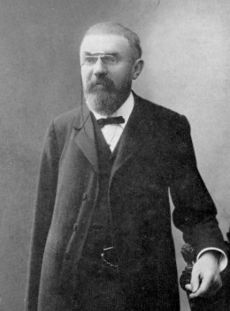
\includegraphics[height=\the\HauteurDesPhotos]{Poincare2}&
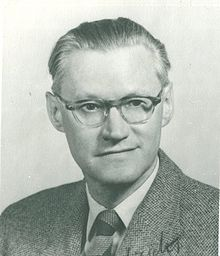
\includegraphics[height=\the\HauteurDesPhotos]{Friedrichs}&
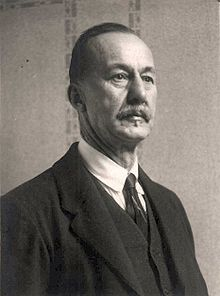
\includegraphics[height=\the\HauteurDesPhotos]{Wirtinger}&
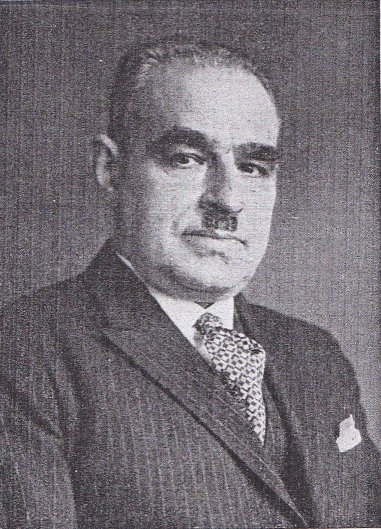
\includegraphics[height=\the\HauteurDesPhotos]{Korn}\\
Poincaré&Friedrichs&Wirtinger&Korn%
\end{tabular}}
\ImageADroite{%
Il est plus connu comme pionnier des télécommunications, plus précisément comme l'inventeur de la téléphotographie. Il met au point un téléautographe, un système de transmission des images fixes à distance, par le biais du fil télégraphique, en recourant aux propriétés photoélectriques du sélénium.}
\end{histoire}

\medskip
\textcolorgreen{%
En mécanique, l'inégalité de Korn\index[aut]{Korn (Arthur), 1870-1945, Allemand} dit que l'énergie élastique (qui est proportionnelle à la norme du tenseur des déformations dans~$L^2(\Omega)$) contrôle (i.e. est supérieure à) la norme du déplacement dans~$H^1(\Omega)$ à l'addition près de la norme du déplacement dans~$L^2(\Omega)$.
Ce dernier point permet de prendre en compte les «mouvements de corps rigides», i.e. les déplacements~$u$ non nuls mais d'énergie élastique nulle.}


% \chapter*{Résumé des outils d'analyse fonctionnelle}
%\addcontentsline{toc}{chapter}{Résumé des outils d'analyse fonctionnelle}

\section*{Norme, produit scalaire, espaces}

Soit~$E$ un \textcolorblue{espace vectoriel}.

\medskip
$\|\cdot\|: E\rightarrow \RR_+$ est une \textcolorblue{norme}\index{norme} sur~$E$ ssi elle vérifie:
\begin{enumerate}
  \item~$(\|x\|=0) \Longrightarrow (x=0)$;
  \item~$\forall\lambda\in\RR, \forall x\in E, \|\lambda x\|=|\lambda|\| x\|, \lambda\in\KK$;
  \item~$\forall x,y\in E, \|x+y\|\le\|x\|+\|y\|$ (inégalité triangulaire).
\end{enumerate}

La \textcolorblue{distance issue de la norme} est la distance définie par~$d(x,y)=\|x-y\|$.\index{distance!issue d'une norme}

\medskip
Toute forme bilinéaire symétrique définie positive\index{Forme!bilinéaire} 
$\langle.,.\rangle: E\times E\rightarrow\RR$ est un \textcolorblue{produit scalaire} sur~$E$.\index{Produit scalaire}
Elle vérifie les propriétés:
\begin{enumerate}
  \item bilinéarité:~$\forall x,y,z\in E, \forall\lambda,\mu\in\RR, \langle x,\lambda y+\mu z\rangle
=\lambda\langle x,y\rangle+\mu\langle x,z\rangle$;
  \item symétrie:~$\forall x,y \in E \quad \langle x\, , \, y \rangle = \langle y\, , \, x\rangle$;
  \item positivité:~$\forall x \in E \quad \langle x\, , \, x \rangle \; \ge \; 0$;
  \item définie:~$\forall x \in E \quad \big(\ \langle x\, , \, x \rangle = 0 \; \Rightarrow x = 0\ \big)$.
\end{enumerate}

La \textcolorblue{norme induite} par le produit scalaire est~$\|x\|=\sqrt{\langle x,x\rangle}$.\index{norme!induite par un produit scalaire}

L'inégalité triangulaire donne alors l'inégalité de Cauchy-Schwarz:~$|\langle x,y\rangle|\le\|x\| \|y\|$.\index{inégalité!de Cauchy-Schwarz}\index[aut]{Cauchy (Augustin Louis, baron -), 1789-1857, Français}\index[aut]{Schwarz (Hermann Amandus), 1843-1921, Allemand}

Un espace vectoriel muni d'une norme est appelé \textcolorblue{espace normé}.\index{espace!vectoriel normé}

Un espace vectoriel muni d'un produit scalaire est appelé \textcolorblue{espace préhilbertien}, \index{espace!préhilbertien}
qui est donc également un espace normé pour la norme induite.

\medskip
Exemple:
Pour~$E = \RR^n$ et~$x = (x_1, ..., x_n)\in\RR^n$, on a les normes:
\[
\|x\|_1=\dsum_{i=1}^n|x_i| \qquad
\|x\|_2= \sqrt{\dsum_{i=1}^nx_i^2} \qquad
\|x\|_\infty=\sup_i|x_i|
\]

Le produit scalaire défini par~$\langle x,y\rangle=\dsum_{i=1}^nx_iy_i$ a pour norme induite
la norme~$\|\cdot\|_2$.

\medskip
Soit~$E$ un espace vectoriel et~$(x_n)_n$ une suite de~$E$. 
$(x_n)_n$ est une \textcolorblue{suite de Cauchy} ssi 
$\forall\varepsilon>0, \exists N, \forall p> N, \forall q> N: \|x_p-x_q\|>\varepsilon$.

Toute suite convergente est de Cauchy. La réciproque est fausse.

Un espace vectoriel est \textcolorblue{complet} ssi toute suite de Cauchy y est convergente.\index{espace!métrique complet}

Un \textcolorblue{espace de Banach} est un espace normé complet.\index{espace!de Banach}\index[aut]{Banach (Stephan), 1892-1945, Polonais}

Un \textcolorblue{espace de Hilbert} est un espace préhilbertien complet.\index{espace!de Hilbert}\index[aut]{Hilbert (David), 1862-1943, Allemand}

Un \textcolorblue{espace euclidien}\index[aut]{Euclide, -325-- -265, Grec} est un espace de Hilbert 
de dimension finie.\index{espace!euclidien}






\medskip
\section*{Espaces fonctionnels}

Un \textcolorblue{espace fonctionnel} est un espace vectoriel dont les éléments sont des
fonctions.

Dans la suite, nous considérons les fonctions définies sur un ouvert~$\Omega\subset\RR^n$ et à
valeurs dans~$\RR$ ou~$\RR^p$.

Un fonction~$u$ est \textcolorblue{mesurable} ssi~$\{x/ |u(x)|<r\}$ est mesurable~$\forall r>0$.

On définit les espaces~$\mathscr{L}^p(\Omega)$, pour~$1\le p<\infty$ par:\index{espace!de Lebesgue}\index[aut]{Lebesgue (Henri-Léon), 1875-1941, Français}
\[
\mathscr{L}^p(\Omega)=\left\{u:\Omega\rightarrow\RR, \text{ mesurable, et telle que }
\dint_\Omega|u|^p<\infty\right\}
\]

\medskip
$L^p(\Omega)$ est la classe d'équivalence des fonctions de~$\mathscr{L}^ p(\Omega)$ 
pour la relation d'équivalence <<égalité presque partout>>: on confondra deux fonctions 
dès qu'elles sont égales presque partout, i.e. lorsqu'elles ne différent que sur un ensemble
de mesure nulle.

Les formes:
\[
\|u\|_{L^p}=\left(\dint_\Omega |u|^p\right)^{1/p}, 1\le p<\infty \qquad \text{ et }
\qquad \|u\|_{L^\infty}=\sup_\Omega |u|
\]
ne sont pas des normes sur~$\mathscr{L}^P(\Omega)$
(en effet, $\|u\|_{L^p}=0$ implique que~$u$ est nulle presque partout dans~$\mathscr{L}^p(\Omega)$
et non pas~$u = 0$, d'où la définition des espaces~$L^p(\Omega)$.

Ces formes sont des normes sur~$L^p(\Omega)$ et en font des espaces de Banach (i.e. complets).\index{norme}\index{espace!de Banach}\index[aut]{Banach (Stephan), 1892-1945, Polonais}

\medskip
Dans le cas particulier~$p=2$, on ontient l'espace~$L^2(\Omega)$ des fonctions de carré 
sommable pp. sur~$\Omega$. On remarque que le norme~$\|u\|_{L^2}=\sqrt{\int_\Omega u^2}$
est induite par le produit scalaire~$(u,v)_{L^2}=\int_\Omega uv$, ce qui fait de
l'espace~$L^2(\Omega)$ un espace de Hilbert.\index{Produit scalaire!de~$L^2$}





\medskip
\section*{Dérivée généralisée}\index{dérivée!généralisée}

Les éléments des espaces~$L^p$ ne sont pas nécessairement des fonctions très régulières.
Leurs dérivées partielles ne sont donc pas forcément définies partout.
C'est pourquoi on va étendre la notion de dérivation. 
Le véritable outil à introduire pour cela est la notion de distribution.
Une idée simplifiée en est la notion de dérivée généralisée (certes plus limitée que
les distributions, mais permettant de sentir les aspects nécessaires pour aboutir aux formulations
variationnelles).

\medskip
\subsection*{Fonctions tests}\index{Fonction!test}

On note~$\mathcal{D}(\Omega)$ l'espace des fonctions de~$\Omega$ vers~$\RR$, de
classe~$C^\infty$, et à support compact inclus dans~$\Omega$.
$\mathcal{D}(\Omega)$ est parfois appelé espace des fonctions-tests.

Théorème: \textcolorred{$\overline{\mathcal{D}(\Omega)}=L^2(\Omega)$}

\medskip
\subsection*{Dérivée généralisée}

Soit~$u\in C^1(\Omega)$ et~$v\in\mathcal{D}(\Omega)$. 
Par intégration par parties (ou Green) on a l'égalité:
\[
\dint_\Omega \partial_iu \varphi = -\dint_\Omega u \partial_i\varphi
+\dint_{\partial\Omega} u\varphi n
= -\dint_\Omega u \partial_i\varphi
\]
(car~$\varphi$ est à support compact donc nulle sur~$\partial\Omega$).

Le terme~$\int_\Omega u \partial_i\varphi$ a un sens dès que~$u\in L^2(\Omega)$,
donc~$\int_\Omega \partial_iu \varphi$ aussi, sans que~$u$ ait besoin d'être~$C^1$.
Il est donc possible de définir~$\partial_i u$ même dans ce cas.

\medskip
Cas~$n=1$: Soit~$I$ un intervalle de~$\RR$, pas forcément borné. 
On dit que~$u\in L^2(I)$ admet une dérivée généralisée dans~$L^2(I)$ 
ssi~$\exists u_1\in L^2(I)$ telle que~$\forall\varphi\in\mathcal{D}(I)$,
$\int_I u_1\varphi = \int_I u\varphi'$.

Par itération, on dit que~$u$ admet une \textcolorblue{dérivée généralisée
d'ordre~$k$} dans~$L^2(I)$, notée~$u_k$, ssi:~$\forall\varphi\in\mathcal{D}(I)$,
$\dint_I u_k\varphi = (-1)^k\dint_I u\varphi^{(k)}$.

Ces définitions s'étendent au cas où~$n>1$.

\medskip
Théorème: Quand elle existe, la dérivée généralisée est unique.

Théorème: Quand~$u$ est de classe~$C^1(\overline{\Omega})$ la dérivée généralisée 
est égale à la dérivée classique.




\medskip
\section*{Espaces de Sobolev}

\medskip
\subsection*{Espaces~$H^m$}\index{espace!de Sobolev~$H^m(\Omega)$}

L'\textcolorblue{espace de Sobolev d'ordre~$m$} est défini par:
\[
H^m(\Omega)=\left\{u\in L^2(\Omega)/ \partial^\alpha u\in L^2(\Omega),
\forall\alpha=(\alpha_1, ..., \alpha_n)\in\NN^n \text{ tel que } |\alpha|=\alpha_1+...+\alpha_n\le m
\right\}
\]

On voit que~$H^0(\Omega)=L^2(\Omega)$.

\medskip
$H^m(\Omega)$ est un espace de Hilbert avec le produit scalaire et la norme induite:\index{norme!sur~$H^m(\Omega)$}\index{norme!induite par un produit scalaire}\index{Produit scalaire!de~$H^m(\Omega)$}
\[
(u,v)_m=\dsum_{|\alpha|\le m}(\partial^\alpha u,\partial^\alpha v)_0 
\quad \text{ et } \quad
\|u\|_m=\sqrt{(u,u)_m}
\]

Théorème: Si~$\Omega$ est un ouvert de~$\RR^n$ de frontière <<suffisament
régulière>>, alors on a l'inclusion:~$H^m(\Omega)\subset C^k(\overline{\Omega})$
pour~$k<m-\frac{n}2$.

\medskip
\subsection*{Trace}\index{espace!trace}

Dans les problèmes physiques que nous rencontrerons (voir partie 2), nous devrons
pouvoir imposer des conditions aux limites.
Ceci est vrai, que l'on s'intéresse aux formulations forte ou faible.

Pour cela, il faut que la valeur d'une fonction sur la frontière soit définie.
C'est justement ce que l'on apelle sa trace. 
La trace est le prolongement d'une fonction sur le bord de l'ouvert~$\Omega$.

De manière analogue, il est possible de prolonger la définition de la dérivée normale
sur le contour de~$\Omega$, ce qui permet de prendre en compte des conditions
aux limites de type Neumann par exemple.


\medskip
\subsection*{Espace~$H^1_0(\Omega)$}\index{espace!trace}\index{espace!de Sobolev~$H_0^1(\Omega)$}

Soit~$\Omega$ ouvert de~$\RR^n$. 
L'espace~$H^1_0(\Omega)$ est défini comme l'adhérence de~$\mathcal{D}(\Omega)$
pour la norme~$\|\cdot\|_ 1$ de~$H^1(\Omega)$.

\medskip
Théorème: Par construction~$H^1_0(\Omega)$ est un espace complet. 
C'est un espace de Hilbert pour la norme~$\|\cdot\|_ 1$.

\medskip
$H^1_0(\Omega)$ est le sous-espace des fonctions de~$H^1(\Omega)$ de trace nulle 
sur la frontière~$\partial\Omega$ (on a:~$H^1_0(\Omega)=\ker\gamma_0$ où~$\gamma_0$
est l'application trace).

\medskip
Pour toute fonction~$u$ de~$H^1(\Omega)$, on peut définir:
\[
|u|_1=\sqrt{\dsum_{i=1}^n\|\partial_i u\|_ 0^2} =
\sqrt{\dint_\Omega\dsum_{i=1}^n (\partial_i u)^2}
\]

\medskip
Inégalité de Poincaré:\index{inégalité!de Poincaré}\index[aut]{Poincaré (Henri), 1854-1912, Français}
Si~$\Omega$ est borné dans au moins une direction, alors il
existe une constante~$C(\Omega)$ telle que~$\forall u\in H^1_0(\Omega)$; 
$\|u\|_0 \le C(\Omega) |u|_1$.
On en déduit que~$|.|_1$ est une norme sur~$H^1_0(\Omega)$, équivalente à 
la norme~$\|\cdot\|_1$.

\medskip
Corollaire: 
Le résultat précédent s'étend au cas où l'on a une condition de Dirichlet nulle
seulement sur une partie de~$\partial\Omega$, si~$\Omega$ est connexe.

\textcolorgris{On suppose que~$\Omega$ est un ouvert borné connexe, de frontière~$C^1$ 
par morceaux. Soit~$V = \{v\in H^1(\Omega); v = 0 \text{ sur } \Gamma_0\}$
où~$\Gamma_0$ est une partie de~$\partial\Omega$ de mesure non nulle. 
Alors il existe une constante~$C(\Omega)$ telle que~$\forall u\in V$;~$\|u\|_{0,V} \le
C(\Omega) |u|_{1,V}$, où~$\|\cdot\|_{0,V}$ et~$|.|_{1,V}$ sont les norme et semi-norme induites 
sur~$V$.
On en déduit que~$|.|_{1,V}$ est une norme sur~$V$ équivalente à la norme~$\|\cdot\|_{1,V}$.}



% \part{Problème continu}
% \chapter{Problèmes physiques: équations différentielles et aux dérivées partielles}
\begin{abstract}
La première partie était uniquement des <<~rappels~>> de notions
mathématiques nécessaires pour disposer d'un certains nombre d'outils.
Maintenant que nous avons ces outils, nous allons nous intéresser
à des problèmes concrêts de la physique (au sens général).

Cette deuxième partie va donc présenter des problèmes physiques,
sous leur forme forte (dans ce chapitre), puis sous forme faible et
variationnelle; la théorie de la formulation faible étant exposée entre temps.
\end{abstract}



\medskip
\section{Introduction}

Une \textcolorblue{équation différentielle} est une relation entre une ou plusieurs fonctions inconnues et 
leurs dérivées. 
\textcolorblue{L'ordre d'une équation différentielle} correspond au degré maximal de dérivation auquel l'une des fonctions inconnues 
a été soumise.

Pour les méthodes explicites de résolution des équations différentielles, on ira voir en annexes.


\medskip
\begin{histoire}%
Les problèmes posés ou menant à des équations différentielles sont aussi vieux que l'analyse elle-même (XVIIe-XVIIIe,
voir notes précédentes sur les fonctions et sur la continuité et la dérivabilité). 
Avant même qu'on ait complètement élucidé la question des infiniment petits 
l'on se préoccupe déjà de résoudre des problèmes de tangente, qui mènent 
invariablement à une équation différentielle. 
Dès les débuts de la mécanique classique, dite newtonienne, on est confronté
à l'intégration de systèmes d'ED du second ordre (voir exemples ci-dessous).

\medskip
On s'habitue progressivement à ce que l'inconnue d'une équation puisse être une fonction, 
même si la fonction a encore à l'époque un statut flou. 

\sbox{\MaBoiteAvecPhotos}{\setlength{\tabcolsep}{0pt}\scriptsize%
\begin{tabular}{cccc}
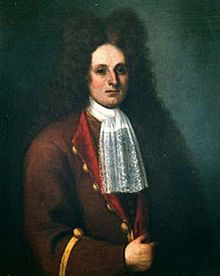
\includegraphics[height=\the\HauteurDesPhotos]{Riccati}&
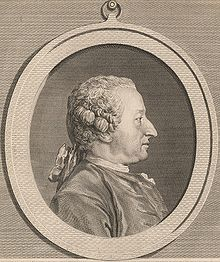
\includegraphics[height=\the\HauteurDesPhotos]{Clairaut}&
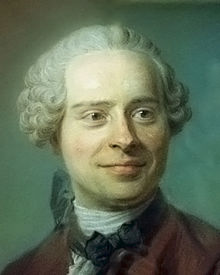
\includegraphics[height=\the\HauteurDesPhotos]{dAlembert}&
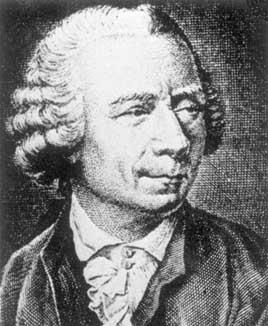
\includegraphics[height=\the\HauteurDesPhotos]{Euler4}\\
Riccati &Clairaut &D'Alembert&Euler%
\end{tabular}}
\bigskip
\ImageADroite{%
On résout les équations différentielles par la méthode des séries entières sans s'encombrer des notions
de convergence, bien que l'on entrevoit parfois certaines difficultés dues justement
à ces problèmes de convergence... et on en arrive presque aux séries asymptotiques 
qui ne seront conceptualisées qu'au XIXe.\\
\indent
Un autre problème reste d'écrire, à l'aide de fonctions simples, les solutions
des équations différentielles.
La liste des équations différentielles que l'on sait résoudre de cette manière est plutôt maigre:
Leibniz\index[aut]{Leibniz (Gottfried Wilhelm), 1646-1716, Allemand}
 et sa méthode de décomposition en éléments simples, les Bernouilli et
les équations différentielles linéaires du premier ordre, puis Riccati...\index[aut]{Riccati (Jacopo Francesco), 1676-1754, Italien}%
}

\medskip
La découverte par Clairaut\index[aut]{Clairaut (Alexis Claude), 1713-1765, Français}
 en 1734 de l'existence d'une solution singulière
à l'équation~$y - xy' + f(y') = 0$ (à la famille de droites~$y = Cx + f(C)$ qui est l'expression 
générale des courbes intégrales, il faut adjoindre l'enveloppe de cette famille pour avoir toutes 
les solutions analytiques de l'équation) relance la dynamique.
D'Alembert,\index[aut]{d'Alembert (Jean le Rond), 1717-1783, Français} 
en 1748, trouve un second cas d'intégrale singulière. 
Mais c'est Euler\index[aut]{Euler (Leonhard Paul), 1707-1783, Suisse} et 
Lagrange\index[aut]{Lagrange (Joseph Louis, comte de -), 1736-1813, Italien} 
qui élucident ce qui se passe en général en exhibant la courbe
qui est le lieu des points singuliers.

\medskip
Si l'on sait, dès la fin du XVIIe siècle intégrer les équations différentielles linéaires du premier et du second ordre 
à coefficients constants par des sommes d'exponentielles, il faut attendre 1760 pour que la 
théorie vienne à bout des équations différentielles linéaires à coefficients constants d'ordre quelconque. 
En 1739, Euler\index[aut]{Euler (Leonhard Paul), 1707-1783, Suisse} 
rencontre une équation différentielle linéaire à coefficients constants du 4e ordre 
sur un problème de vibration des tiges qu'il ne sait pas intégrer. 
C'est en 1743 qu'il forme ce qu'on appelle aujourd'hui l'équation caractéristique, qu'il complète
un peu plus tard lorsqu'une racine de cette équation polynomiale est multiple.

\sbox{\MaBoiteAvecPhotos}{\setlength{\tabcolsep}{0pt}\scriptsize%
\begin{tabular}{cccc}
\includegraphics[height=\the\HauteurDesPhotos]{Lagrange2}&
\includegraphics[height=\the\HauteurDesPhotos]{Laplace}&
\includegraphics[height=\the\HauteurDesPhotos]{Sturm}&
\includegraphics[height=\the\HauteurDesPhotos]{Liouville}\\
Lagrange &Laplace &Sturm&Liouville%
\end{tabular}}
\medskip
\ImageADroite{%
D'Alembert\index[aut]{d'Alembert (Jean le Rond), 1717-1783, Français} 
remarque que pour les équations différentielles non homogènes, l'adjonction d'une solution particulière 
à la solution générale de l'équation homogène donne la solution générale de l'équation homogène.
Lagrange\index[aut]{Lagrange (Joseph Louis, comte de -), 1736-1813, Italien} 
introduit la méthode de variation des constantes pour résoudre par quadratures l'équation 
linéaire non homogène lorsque l'on connaît la solution générale de l'équation homogène. 
}

\medskip
Clairaut, D'Alembert, Euler, Lagrange et Laplace consacrent de nombreux mémoires au problème
des~$n$ corps.
Le premier exemple du problème de Sturm-Liouville\index[aut]{Sturm (Jacques Charles François), 1803-1855, Français}\index[aut]{Liouville (Joseph), 1809-1882, Français}
 est donné par D'Alembert\index[aut]{d'Alembert (Jean le Rond), 1717-1783, Français} 
à propos de la vibration d'une corde non homogène.
\end{histoire}

\medskip
Les mathématiciens du XVIIIe siècle admettent sans discussion l'existence de solutions des 
ED et EDP sans chercher le domaine d'existence de ces solutions.
Il faut attendre Cauchy,\index[aut]{Cauchy (Augustin Louis, baron -), 1789-1857, Français} 
vers 1820, pour que soit abordée l'existence d'une solution à 
l'ED~$y' = f(x,y)$, où~$f$ est supposée continument différentiable en chaque variable.
Sans connaître les travaux de Cauchy, Lipschitz,\index[aut]{Lipschitz (Rudolph Otto Sigismund), 1832-1903, Allemand} 
en 1868, retrouve le résultat de Cauchy mais, s'affranchit de l'hypothèse de différentiabilité 
de~$f$ au profit de la condition dite aujourd'hui de Lipschitz.
En 1837, Liouville\index[aut]{Liouville (Joseph), 1809-1882, Français} 
utilise, pour le cas particulier d'une équation linéaire du second ordre une 
méthode d'approximation successive: on construit une suite de fonctions convergeant
vers la solution.
\colorblack


\medskip
Si l'on considère une fonction~$f$, sa dérivée~$f'$ exprime sa variation: 
positive~$f$ est croissante (et plus sa value est grande, plus la croissance est rapide), 
négative~$f$ est décroissante...

À partir de là on peut considérer une population de personnes. Le nombre de total
de personnes à un instant~$t$ est donné par~$f(t)$.
Plus la population est nombreuse, plus elle se reproduit: en d'autres termes, la
vitesse de croissance de la population est proportionnelle à la taille de la population.
On peut donc écrire: \begin{equation} %$\colorgreen
f'(t)=k\,f(t)\end{equation}%$.
C'est une équation différentielle très simple, mais qui modélise le problème dit de dynamique de population.\index{ED-EDP!dynamique de population}

\medskip
Un autre problème simple, toujours en dynamique des populations, est celui de deux
populations interdépendantes: les proies~$g(t)$ et le prédateurs~$m(t)$.
Les proies se reproduisent et sont mangées par les prédateurs, alors que
les prédateurs meurent sauf s'ils peuvent manger des proies.

Cela conduit au système de Lotka-Volterra:\index{ED-EDP!Lotka-Volterra}\index{ED-EDP!système proie-prédateur}\index[aut]{Volterra (Vito), 1860-1940, Italien}\index[aut]{Lotka (Alfred James), 1880-1949, Américain}
\begin{equation}%$\colorgreen
  \begin{cases} g'(t)&=A\,g(t)-B\,g(t)\,m(t) \\ m'(t)&=-C\,m(t)+D\,g(t)\,m(t) \end{cases} 
\end{equation}
où il est nécessaire de résoudre les équations simultanément (on dit que les équations
sont couplées)

\medskip
Pour revenir à des exemples plus connus du lecteurs, on n'oubliera pas que
la relation fondamentale de la dynamique, de Newton: \begin{equation} %$\colorgreen
m\ddot{x}=f(x)\end{equation}%$
est une d'ED du second ordre.\index{ED-EDP!relation fondamentale de la dynamique}\index[aut]{Newton (Isaac, Sir -), 1643-1727, Anglais}

On pourrait multiplier les exemples comme l'équation de l'oscillation d'une masse
suspendue à un ressort: \begin{equation}%~$\colorgreen
\ddot{x} = - c \dot{x} - \omega^2x \end{equation}%$
avec ($c>0$) ou sans ($c=0$) frottement.\index{ED-EDP!oscillation d'une masse suspendue à un ressort}

\medskip
Comme on le voit sur les exemples ci-dessus, et comme on s'en souvient sans doute,
il est nécessaire, pour déterminer complètement la solution d'une équation différentielle (ou d'une équation aux dérivées partielles),
de disposer de valeurs de la solution en certains points.
On appelle ces <<~contraintes~>>, des \textcolorblue{conditions aux limites}.

Les conditions aux limites types sont présentées au paragraphe suivant.


\medskip
\begin{histoire}%
Concernant les équations aux dérivées partielles, elles sont initialement résolues par des méthodes ad-hoc, le plus souvent 
géométriques. 
On n'écrit pas l'équation aux dérivées partielles linéaires. On ne s'étonnera donc pas que la première équation aux dérivées partielles 
n'apparaisse qu'assez tard.

\sbox{\MaBoiteAvecPhotos}{\setlength{\tabcolsep}{0pt}\scriptsize%
\begin{tabular}{cccc}
\includegraphics[height=\the\HauteurDesPhotos]{Cauchy3}&
\includegraphics[height=\the\HauteurDesPhotos]{Lipschitz2}&
\includegraphics[height=\the\HauteurDesPhotos]{Dirichlet2}&
\includegraphics[height=\the\HauteurDesPhotos]{Neumann}\\
Cauchy&Lipschitz&Dirichlet&Neumann%
\end{tabular}}
\medskip
\ImageADroite{%
La théorie de l'intégration des équations aux dérivées partielles du premier ordre ne date que de 1734. 
L'idée d'Euler\index[aut]{Euler (Leonhard Paul), 1707-1783, Suisse} 
est de ramener ladite intégration à celle des équations différentielles ordinaires. 
Euler montre qu'une famille de fonctions dépendant de deux paramètres vérifie une 
EDP du premier ordre en éliminant ces paramètres entre les dérivées partielles. 
Inversement, une telle équation admet une solution dépendant d'une fonction arbitraire. 
Il parvient ainsi à intégrer plusieurs équations de ce type.
}

\medskip
Lagrange,\index[aut]{Lagrange (Joseph Louis, comte de -), 1736-1813, Italien} 
dans un mémoire de 1785, résume les connaissances de l'époque sur ces questions. 
Il ne sait intégrer que onze types d'équations aux dérivées partielles du premier ordre.

\medskip
La solution de l'intégration de ces équations allait venir d'un mathématicien peu connu, 
mort en 1784, Paul Charpit.\index[aut]{Charpit de Villecourt (Paul), ?-1784, Français}
Son mémoire, présenté en 1784 à l'académie des sciences n'a 
jamais été publié et est resté longtemps une énigme. Une copie de ce mémoire a été
trouvée en 1928.
\end{histoire}
\colorblack

\medskip
\section{Conditions aux limites}\index{Conditions aux limites}

Comme nous venons de le dire, les \textcolorblue{conditions aux limites} sont des
contraintes (des valeurs) que l'on impose à la fonction solution (ou à certaines de
ces dérivées) sur tout ou partie du domaine~$\Omega$, et/ou sur toute ou partie 
de sa frontière~$\Gamma=\partial\Omega$.

D'un point de vue <<~vocabulaire~>>, certains types de conditions aux limites standard
existent qui sont listées ci-après.

\medskip
\subsection{Dirichlet -- valeurs aux bords}\index{Conditions aux limites!de Dirichlet}\index[aut]{Dirichlet (Johann Peter Gustav Lejeune), 1805-1859, Allemand}

On parle de \textcolorblue{condition de Dirichlet} imposée à une équation différentielle ou une équation aux dérivées partielles,
lorsque l'on spécifie les \textcolorred{valeurs} que la solution doit vérifier sur toute ou partie de
la frontière du domaine.

\medskip
Il peut s'agir par exemple d'un déplacement imposé (par exemple nul) en des points
d'une structure (points d'appuis rigides).

\medskip
\subsection{Neumann -- gradients aux bords}\index{Conditions aux limites!de Neumann}\index[aut]{Neumann (Carl Gottfried), 1832-1925, Allemand}

On parle de \textcolorblue{condition de Neumann} imposée à une équation différentielle ou une équation aux dérivées partielles,
lorsque l'on spécifie les \textcolorred{valeurs des dérivées} que la solution doit vérifier sur la frontière du 
domaine (flux, contraintes...)

\medskip
\subsection{Robin -- relation gradient/valeurs sur le bord}\index{Conditions aux limites!de Robin}\index[aut]{Robin (Victor Gustave), 1855-1897, Français}

On parle de \textcolorblue{condition de Robin} ou \textcolorblue{condition de Fourier} 
ou \textcolorblue{condition d'impédance} imposée à une équation différentielle ou une équation aux dérivées partielles,
lorsque l'on spécifie une \textcolorred{relation linéaire} entre les valeurs de la fonction et les
valeurs de la dérivée de la fonction qui est solution du problème sur toute ou partie de
la frontière du domaine.

C'est donc une pondérations de conditions de Dirichlet et de Neumann.

\medskip
\subsection{Condition aux limites dynamique}\index{Conditions aux limites!dynamique}

On parle de \textcolorblue{condition aux limites dynamique} imposée à une équation différentielle ou une équation aux dérivées partielles,
lorsque l'on spécifie une \textcolorred{combinaison linéaire} entre la dérivée temporelle et 
la dérivée normale que la solution doit vérifier sur toute ou partie la frontière du 
domaine.

\medskip
\subsection{Condition aux limites mêlée}\index{Conditions aux limites!mêlée}

On parle de \textcolorblue{condition aux limites mêlée} lorsque l'on juxtapose
plusieurs conditions aux limites différentes sur toute ou partie de la frontière du 
domaine.






\medskip
\section{Types d'équations aux dérivées partielles}

La forme générale d'une équation aux dérivées partielles linéaire, scalaire, d'ordre 2 est:
\begin{equation}
au + c \nabla u + \dive (A\nabla u) = f
\end{equation}
où~$a: \Omega\rightarrow\RR$, $c: \Omega\rightarrow\RR^n$, 
$A: \Omega\rightarrow\RR^{n\times n}$ et~$f: \Omega\rightarrow\RR$ sont
les coefficients de l'équation aux dérivées partielles linéaires.

\medskip
Dans le cas où~$u$ est scalaire ($n = 1$) et les coefficients sont constants, on obtient:
\begin{equation}
\alpha\dfrac{\partial^2 u}{\partial x^2}+\beta\dfrac{\partial^2 u}{\partial x\partial y}
+\gamma \dfrac{\partial^2 u}{\partial y^2} + \delta \dfrac{\partial u}{\partial x}
+ \epsilon \dfrac{\partial u}{\partial y} +\gamma u = f
\end{equation}
où~$\alpha$, $\beta$, $\gamma$, $\delta$, $\epsilon$, $\gamma$ sont des scalaires.

Cette équation est dite:
\begin{itemize}
  \item \textcolorblue{elliptique} si~$\beta^2-4\alpha\gamma>0$;
  \item \textcolorblue{parabolique} si~$\beta^2-4\alpha\gamma=0$;
  \item \textcolorblue{hyperbolique} si~$\beta^2-4\alpha\gamma<0$.
\end{itemize}

\medskip
\colorgreen
On peut dire que:
\begin{itemize}
  \item les problèmes elliptiques vont concerner les problèmes de la mécanique;
  \item les problèmes paraboliques ceux de type équation de la chaleur;
  \item les problèmes hyperboliques ceux de la propagation des ondes.
\end{itemize}
\colorblack

\medskip
\section{Phénomènes de propagation et de diffusion}


Dans ce paragraphe, nous avons regroupé les notions de propagation
et de diffusion.

La propagation est la diffusion sont liées.
La diffusion, c'est en quelque sorte l'homogénéisation d'une grandeur dans un milieu et
dans le temps.
Or pour qu'il y ait diffusion, il faut bien que ledit phénomène se propage.


\medskip
\begin{histoire}%
Le déplacement des atomes, ions ou molécules dans un milieu, que celui-ci soit solide (cristallin ou amorphe), 
liquide ou gazeux, est appelé de manière générale <<~migration~>>. 

\sbox{\MaBoiteAvecPhotos}{\setlength{\tabcolsep}{0pt}\scriptsize%
\begin{tabular}{cc}
\includegraphics[height=\the\HauteurDesPhotos]{Brown}&
\includegraphics[height=\the\HauteurDesPhotos]{Fick}\\
Brown&Fick%
\end{tabular}}
\medskip
\ImageADroite{%
Au sens large la diffusion désigne des transferts obéissant aux lois de Fick,\index[aut]{Fick (Adolf Eugene), 1829-1901, Allemand} 
i.e. dont la résultante macroscopique vérifie l'équation de diffusion. 
La turbulence entraine ainsi une forte diffusion dans les fluides. 
La diffusion moléculaire est la migration sous l'effet de l'agitation thermique, à l'exception des autres 
phénomènes. 
Elle intervient par exemple dans des procédés d'amélioration des caractéristiques mécaniques 
(traitements de surface comme la nitruration ou cémentation), la résistance à la corrosion et les 
procédés d'assemblage par brasage.
}

\medskip
En 1827, le botaniste Robert Brown\index[aut]{Brown (Robert), 1773-1859, Écossais} 
observe le mouvement erratique de petites particules de pollen 
immergées dans de l'eau. Il ne s'agit pas d'un phénomène de diffusion, puisque ce qui bouge est 
une particule macroscopique, mais cette <<~marche aléatoire~>>, que l'on appellera <<~mouvement 
brownien~>>, servira de modèle pour la diffusion:
Le mouvement brownien, ou processus de Wiener, 
est le mouvement aléatoire d'une <<~grosse~>> particule immergée dans un fluide et qui n'est soumise 
à aucune autre interaction que des chocs avec les <<~petites~>> molécules du fluide environnant. 
Il en résulte un mouvement très irrégulier de la grosse particule.
Ce mouvement, qui permet de décrire avec succès le comportement thermodynamique des gaz 
(théorie cinétique des gaz), est aussi très utilisé dans des modèles de mathématiques financières.

\medskip
En 1855, Adolph Fick\index[aut]{Fick (Adolf Eugene), 1829-1901, Allemand} 
propose des lois phénoménologiques, empiriques, inspirées de la loi de 
Fourier\index[aut]{Fourier (Jean Baptiste Joseph), 1768-1830, Français} 
pour la chaleur (établie en 1822). 
C'est Albert Einstein\index[aut]{Einstein (Albert), 1879-1955, Suisse-américain} 
qui démontrera les lois de Fick\index[aut]{Fick (Adolf Eugene), 1829-1901, Allemand} 
en 1905 avec ses travaux sur la loi stochastique. 
La première loi de Fick énonce que <<~le flux de diffusion est proportionnel au gradient de 
concentration~>>.
\end{histoire}
\colorblack

\medskip
Nous nous placerons dans un cadre beaucoup plus macroscopique, où les interactions
entre particules sont quantifiées au travers de variables macroscopiques continues, comme
par exemple la température, la pression, mais également le frottement fluide, la
conductivité thermique, la masse volumique...

L'analogie de formulation mathématique nous fera également considérer les cas
de propagation des ondes dans des milieux donnés.
C'est d'ailleurs essentiellement via la propagation des ondes que nous aborderons
les formulations... l'équation de la chaleur constituant le liant idéal pour illustrer
les liens entre propagation et diffusion.

\medskip
\subsection{Équations de Laplace et Poisson}
L'\textcolorblue{équation de Laplace, ou Laplacien} est l'équation:\index{ED-EDP!de Laplace}\index[aut]{Laplace (Pierre Simon de -), 1749-1827, Français}\index{Laplacien}
\begin{equation}\Delta \varphi=0\end{equation}
Elle est elliptique.

Elle apparaît dans de nombreux problèmes physiques: astronomie, électrostatique, 
mécanique des fluides, propagation de la chaleur, diffusion, mouvement brownien, mécanique quantique.

Les fonctions solutions de l'équation de Laplace sont appelées les \textcolorblue{fonctions harmoniques}.
Toute fonction holomorphe est harmonique.

\medskip
L\textcolorblue{'équation de Poisson} est l'équation:\index{ED-EDP!de Poisson}\index[aut]{Poisson (Siméon Denis), 1781-1840, Français}
\begin{equation}\Delta \varphi=f\end{equation}
où~$f$ est une fonction donnée. Elle est elliptique.

\medskip
Par exemple, en électrostatique, on exprime le potentiel électrique~$V$ associé à une distribution 
connue de charges~$\rho$ (dans le vide) par la relation:
\begin{equation}
  \Delta V = - \dfrac{\rho}{\epsilon_0}
\end{equation}

En gravitation universelle, le potentiel gravitationnel~$\Phi$ est relié à la masse volumique 
$\mu$ par la relation:
\begin{equation}
\Delta \Phi = 4 \pi \, G \, \mu 
\end{equation}

\medskip
\subsection{Équation d'onde, phénomènes vibratoires}

Il s'agit encore d'une extension de l'équation de Laplace.

L'\textcolorblue{équation d'onde} est l'équation générale qui décrit la propagation d'une onde
(sonore ou électromagnétique dont la lumière),
qui peut être représentée par une grandeur scalaire ou vectorielle.


Dans le cas vectoriel, en espace libre, dans un milieu homogène, linéaire et isotrope, l'équation d'onde s'écrit:\index{ED-EDP!des ondes}
\begin{equation}
  \Delta u \ = - \frac1{c^2} \dfrac{\partial^2 u}{\partial t^2} \quad \text{ ou} \quad \square u =0
\end{equation}
où la fonction d'onde inconnue est notée~$u(x,y,z,t)$, $t$ représente le temps, et 
le nombre~$c$ représente la célérité ou vitesse de propagation de l'onde~$u$ 
(rappel:~$\square$ est le d'Alembertien). Elle est hyperbolique.

\medskip
Dans le cas de \textcolorblue{l'acoustique}, alors cette équation est obtenue à partir des 
équations de la mécanique ainsi que de l'hypothèse de fluide parfait:
\begin{itemize}
  \item conservation de la masse:~$\dot{\rho}+\dive(\rho u)=0$ avec
	$\rho$ la masse volumique du milieux et~$u$ sa vitesse;
  \item conservation de la quantité de mouvement:~$\dive(\sigma)=\rho\dot{u}$, avec
	$\sigma$ le tenseur des contraintes
  \item le fluide est parfait, et sa relation de comportement est donc:~$\sigma=-p'I$ avec
	$p'$ la pression dans le fluide.
\end{itemize}

À partir de ces trois équations, on retrouve l'équation des ondes sous la forme:\index{ED-EDP!de l'acoustique}
\begin{equation}
\Delta p' - \dfrac1{c^2} \ddot{p}' = 0
\end{equation}
avec~$c$ la célérité de l'onde acoustique dans le milieu (vitesse du son).

\medskip
L'équation des ondes permet également de modéliser le problème de l'évolution 
de la déformation d'une membrane tendue (peau de tambour).\index{ED-EDP!de la déformation d'une membrane}
Dans ce cas là, on note plutôt:
\begin{equation}
 \sigma \Delta u = \rho\ddot{u} \text{ dans}\Omega
\end{equation}
où~$\Omega$ est notre domaine qui est une surface, donc~$\Omega\subset\RR^2$.

\textcolorblue{La même équation en dimension deux ou trois modélise la plupart des phénomènes 
vibratoires.}
En dimension 1, cette équation s'appelle l'\textcolorblue{équation des cordes vibrantes.}



%É
\medskip
\subsection{Équation de la chaleur}

L'\textcolorblue{équation de la chaleur} est une équation aux dérivées partielles parabolique, introduite initialement en 1811 par Fourier 
pour décrire le phénomène physique de conduction thermique.\index{ED-EDP!de la chaleur}\index[aut]{Fourier (Jean Baptiste Joseph), 1768-1830, Français}

\medskip
\begin{histoire}%
\textbf{À propos de l'effet régularisant de la chaleur:}

L'équation de la chaleur a un <<~effet régularisant~>>:
quelque soit la distribution initiale de la température pour un problème donné,
même discontinue, on aboutit rapidement à une distribution continue et même
lisse de la température.

\sbox{\MaBoiteAvecPhotos}{\setlength{\tabcolsep}{0pt}\scriptsize%
\begin{tabular}{ccc}
\includegraphics[height=\the\HauteurDesPhotos]{Nirenberg}&
\includegraphics[height=\the\HauteurDesPhotos]{Nash}&
\includegraphics[height=\the\HauteurDesPhotos]{DeGiorgi}\\
Nirenberg&Nash&De Giorgi%
\end{tabular}}
\medskip
\ImageADroite{%
En 1956, Louis Nirenberg\index[aut]{Nirenberg (Louis), 1925- , Américain} 
propose un nouveau problème à John Nash\index[aut]{Nash (John Forbes), 1928- , Américain} 
(qui est <<~aussi pressé que X, aussi exaspérant que Y, quels que soient X et Y~>> selon
Warren Ambrose): la continuité des solutions de l'équation de la chaleur dans
les milieux discontinus, i.e. lorsque le coefficient de conductivité est quelconque,
et peut même varier brutalement d'un point à l'autre et que l'on a seulement des
bornes inférieure et supérieure sur la conductivité.
}

\medskip
John Nash\index[aut]{Nash (John Forbes), 1928- , Américain} 
résout le problème, notamment à l'aide du concept d'entropie de 
Boltzmann,\index[aut]{Boltzmann (Ludwig), 1944-1906, Autrichien} 
mais n'obtiendra pas le triomphe escompté, le problème ayant été résolu, en même temps, 
mais par une autre méthode, par l'italien De Giorgi,\index[aut]{De Giorgi (Ennio), 1928-1996, Italien} 
qui lui deviendra célèbre (mais John Nash\index[aut]{Nash (John Forbes), 1928- , Américain} 
est célèbre pour d'autres travaux... prix Nobel d'économie en 1994, voir
le film <<~un homme d'exception~>> (A Beautiful Mind) de Ron Howard\index[aut]{Howard (Ronald William), 1954- , Américain} 
en 2001).
\end{histoire}
\colorblack

\medskip
Soit~$\Omega$ un domaine de~$\RR^3$ de frontière~$\Gamma=\partial \Omega$ et~$T(x,t)$ 
un champ de température sur ce domaine (champ de scalaires). 
En présence d'une source thermique dans le domaine, et en l'absence de convection, i.e.
de transport de chaleur (i.e. on s'intéresse à la propagation de la température au sein d'un 
milieu <<~stable~>>, \textcolorgreen{i.e. qui ne bouge pas; on ne s'intéresse pas à la propagation de chaleur
due par exemple à l'existence d'un courant d'air, d'un courant de convection. La convection
est plutôt un problème de mécanique des fluides.)}, 
l'équation de la chaleur s'écrit:
\begin{equation}
\forall x \in\Omega, \quad \frac{\partial T (x,t)}{\partial t} = D \, \Delta T(x,t) + \frac{f}{\rho c}
\end{equation}
où:
\begin{itemize}
  \item~$\Delta$ est l'opérateur Laplacien;
  \item~$D$ est le coefficient de diffusivité thermique (en~$m^2/s$);
  \item~$f$ une éventuelle production volumique de chaleur (en~$W/m^3$);
  \item~$\rho$ est la masse volumique du matériau (en~$kg/m^3$);
  \item~$c$ la chaleur spécifique massique du matériau (en~$J/kg·K$).
\end{itemize}

\medskip\colorgris
L'équation de la chaleur est donc une équation de la forme:
\begin{equation}
\dot{u}-\Delta u=f
\end{equation}
Elle est parabolique.\colorblack

\medskip
Pour que le problème soit bien posé, il faut spécifier:
\begin{itemize}
  \item une condition initiale:~$\forall x\in\Omega, \quad T (x,0) = T_0(x)~$;
  \item une condition aux limites sur le bord du domaine, par exemple:

    de Dirichlet:~$\forall x\in\partial \Omega, \quad T (x,t) = 0~$;

    ou de Neumann:~$\forall x\in\partial \Omega, \quad \frac{\partial T (x,t)}{\partial n} \ 
	= n(x) \cdot \nabla T(x,t) = 0$, où~$n(x)$ est le vecteur normal unitaire au point~$x$.
\end{itemize}

\medskip
L'équation de la chaleur, introduite initialement pour décrire la conduction thermique, permet
de décrire le phénomène de diffusion.

La diffusion est un phénomène de transport irréversible qui se traduit à terme
par une homogénéisation de la grandeur considérée (par exemple la température
dans un domaine, la concentration en produits chimiques dans une solution...).

D'un point de vue phénoménologique, et au premier ordre, ce phénomène est régi par une 
\textcolorblue{loi de Fick} (par exemple sorption d'eau dans les matériaux composites, diffusion d'actifs au travers
de la peau).\index[aut]{Fick (Adolf Eugene), 1829-1901, Allemand}
Dans l'équation précédente, $T$ représente alors la répartition de la grandeur
considérée (eau dans un composite, concentration d'un constituant chimique...) et 
le terme source dans~$\Omega$ est souvent nul (i.e.~$f=0$).





\medskip
\section{Mécanique des fluides}
La mécanique des fluides est une des deux composantes de la mécanique des milieux continus;
l'autre composante étant la mécanique des solides qui sera traitée un peu plus loin.





\medskip
\subsection{Équation de Navier-Stokes}

\begin{histoire}%
Des 23 problèmes de Hilbert\index[aut]{Hilbert (David), 1862-1943, Allemand} 
énoncés en 1900, la moitié est aujourd'hui complètement
résolue, l'un a été démontré indécidable, cinq ne le sont pas du tout, les autres 
étant partiellement traités.

\sbox{\MaBoiteAvecPhotos}{\setlength{\tabcolsep}{0pt}\scriptsize%
\begin{tabular}{cccc}
\includegraphics[height=\the\HauteurDesPhotos]{Navier}&
\includegraphics[height=\the\HauteurDesPhotos]{Stokes}&
\includegraphics[height=\the\HauteurDesPhotos]{Perelman}\\
Navier &Stokes &Perelman%
\end{tabular}}

\medskip
\ImageADroite{%
Des 7 problèmes de l'institut Clay (ou problèmes du prix du millénaire, dotés chacun
d'un million de dollars américains) énoncés en 2000, seule la conjecteure de Poincaré\index[aut]{Poincaré (Henri), 1854-1912, Français} 
a été démontrée en 2003 par Grigori Perelman\index[aut]{Perelman (Grigori Iakovlevitch), 1966- , Russe} 
(qui a refusé le prix, ainsi que la médaille Field. D'ailleurs il n'a pas publié son
travail dans un journal, mais l'a rendu publique et gratuit sur internet...).
Notons au passage que Grigori Perelman\index[aut]{Perelman (Grigori Iakovlevitch), 1966- , Russe} 
est analyste, i.e. un spécialiste des équations aux dérivées partielles, un sujet que beaucoup de topologues avaient 
l'habitude de regarder de loin. Ils ont changé d'avis depuis! 
}

\sbox{\MaBoiteAvecPhotos}{\setlength{\tabcolsep}{0pt}\scriptsize%
\begin{tabular}{c}%
\includegraphics[height=30mm]{Ricci.eps}%
\end{tabular}}
\medskip
\ImageAGauche{%
Pour information, la preuve de Perelman suit le programme de Hamilton,\index[aut]{Hamilton (Richard Streit), 1943-, Américain}
qui le premier a pensé à utiliser le flot de Ricci\index[aut]{Ricci-Curbastro (Gregorio), 1853-1925, Italien} pour s'attaquer
à ce problème.
Deux mots en aparte sur le flot de Ricci dont on entend beaucoup parlé en ce moment...
Regardons se qui se passe dans le plan. On part d'une courbe (au centre de l'image ci-contre) qui
est <<~biscournue~>> et peut même comporter des boucles.
Si on la modifie de sorte que chacun de ses points est bougé proportionnellement à sa courbure,
alors on obtient une seconde courbe, un peu plus lisse... et en itérant le procédé, on
finit par retomber sur un cercle (i.e. sur une sphère en dimension 2), et donc on <<~voit~>>
que la conjecture de Poincaré\index[aut]{Poincaré (Henri), 1854-1912, Français} est vraie.
En d'autres termes, le flot de Ricci permet d'homogénéiser la courbure de la courbe (de la variété dans le
cas général).
}

\medskip
Le problème des équations de Navier-Stokes\index[aut]{Navier (Claude Louis Marie Henri), 1785-1836, Français}\index[aut]{Stokes (George Gabriel), 1819-1903, Anglais}
 figure parmi ces 7 problèmes, c'est dire
si le problème n'est pas simple. Et c'est, des 7 problèmes du millénaire, le seul
qui soit en lien direct avec la physique (en lien très direct...).
De plus, l'Institut Clay n'a pas fixé comme objectif la démonstration de l'existence
de solutions pour les équations de Navier-Stokes et la démonstration que les solutions,
si elles existent, sont uniques. Il a <<~simplement~>> proposé de récompenser des
<<~progrès essentiels~>> sur le sujet.
Pourtant des calculs en mécaniques des fluides sont effectués chaque jour, par exemple
au sein de bureaux d'études pour dimensionner des voitures en aérodynamique.

On n'a pas pu prouver, pour ces équations, qu'il existe en toutes circonstances une
solution parfaitement déterminée par les conditions initiales. 
Pour expliquer sommairement où réside la difficulté avec ces équations,
on pourait dire qu'avec les équations de Navier-Stokes, on passe du discret au continu.

\medskip
Le problème c'est que l'on n'est pas sûr que ce qui est calculé est réellement une
solution approchée et si le résultat est fidèle à la réalité: nous nous trouvons dans
un cas où l'existence et l'unicité des solutions n'est pas facile à prouver.
S'il existe des cas où des solutions régulières parfaitement déterminées à partir des
conditions aux limites, cela n'est pas vrai en toutes circonstances et pour tous temps (on
ne sait pas si une solution régulière ne peut pas devenir turbulente près un temps
suffisamment long par exemple).

\sbox{\MaBoiteAvecPhotos}{\setlength{\tabcolsep}{0pt}\scriptsize%
\begin{tabular}{cc}
\includegraphics[height=\the\HauteurDesPhotos]{Boltzmann}&
\includegraphics[height=\the\HauteurDesPhotos]{Villani}\\
Boltzmann&Villani%
\end{tabular}}
\medskip
\ImageADroite{%
La non linéarité de ces équations joue des tours conduisant à des solutions qui peuvent
par exemple ne pas se superposer sans s'influencer (alors que ce n'est pas le cas avec les équations
linéaires). La viscosité n'est pas exempte de problème non plus, puisqu'elle conduit
aux turbulences (que l'on pourrait qualifier de problème de passage d'échelle). 
D'ailleurs une description à un niveau intermédiaire entre une description atomiste 
(microscopique) et une description continue (macroscopique) a été faite par Boltzmann\index[aut]{Boltzmann (Ludwig), 1944-1906, Autrichien} 
(niveau mésoscopique, description statistique), mais nous ne la présenterons pas ici.
Les travaux de Cédric Villani\index[aut]{Villani (Cédric), 1973- , Français}
 (médaillé Fields 2010) ont répondu en grande 
partie au problème de la théorie cinétique (qui décrit un système constitué d'un très 
grand nombre de particules en interaction).
Il a également prouvé des formes quantifiées du second principe de la thermodynamique: 
Boltzmann avait prouvé la croissance de l'entropie, et Cédric Villani en collaboration avec 
Laurent Desvillettes\index[aut]{Desvillettes (Laurent), 1966- , Français} 
et Giuseppe Toscani\index[aut]{Toscani (Giuseppe), ?- , Italien} 
a permis de quantifier la production d'entropie et le retour à l'équilibre.
Ses travaux sur l'effet Landau\index[aut]{Landau (Lev Davidovitch), 1908-1968, Russe} 
(phénomène de relaxation non collisionnelle) ont des 
répercussions théoriques et pratiques, par exemple dans les modèles de mécanique classique 
en astrophysique.
}

\medskip
La description faible du problème, qui sera présentée dans un autre chapitre,
comporte elle-aussi ses problèmes car on n'est pas sûr de la convergence vers
la solution forte.

Bien que des résultats d'existences et d'unicité existent, aucun ne permet soit de
conclure à l'existence de solutions régulières pour tout temps, soit à l'apparition
de singularité... On retrouve ici la notion de chaos, déterministe ou non, que nous n'aborderons
pas dans ce document, mais pour lequel il est aisé de trouver de la documentation.
Signalons quand même qu'il est identique de parler de dynamique non linéaire ou
de théorie du chaos. On pourra donc se servir de ces deux points d'entrée pour toute
recherche sur le sujet.
\end{histoire}
\colorblack


\medskip
Les équations de Navier-Stokes sont des équations aux dérivées partielles non linéaires qui décrivent le mouvement 
des fluides newtoniens (visqueux) dans l'approximation des milieux continus. 
Elles modélisent par exemple les mouvements de l'air de l'atmosphère, les courants océaniques, 
l'écoulement de l'eau dans un tuyau, et de nombreux autres phénomènes d'écoulement de fluides.

\medskip
Nous considérons l'équation de Navier-Stokes sous la forme:\index{ED-EDP!de Navier-Stokes}\index[aut]{Navier (Claude Louis Marie Henri), 1785-1836, Français}\index[aut]{Stokes (George Gabriel), 1819-1903, Anglais}
\begin{equation}
\rho \dot{u} + \rho (u\cdot\nabla)u - \eta \Delta u
- \left( \zeta + \frac{\eta}{3} \right) \gradb (\dive u)
= \rho f - \nabla p
\end{equation}
où:
\begin{itemize}
  \item~$u$ est la vitesse du fluide ;
  \item~$p$ est la pression dans le fluide ;
  \item~$\rho$ est la masse volumique du fluide;
  \item~$\eta$ est la viscosité dynamique en cisaillement du fluide;
  \item~$\zeta$ est la viscosité dynamique en compression du fluide;
  \item~$f$ est une force massique s'exerçant dans le fluide (par exemple: pesanteur).
\end{itemize}

\medskip
Si de plus le fluide est incompressible (bonne approximation pour les liquides), alors~$\dive u = 0$ 
et l'équation se simplifie:
\begin{equation}
\rho \dot{u} + \rho (u\cdot\nabla)u - \eta \Delta u
= \rho f - \nabla p
\end{equation}



\medskip
\subsection{Équation de Stokes}

Il s'agit d'un cas particulier de l'équation de Navier-Stokes (termes inertiels absents ou négligés).

Lorsqu'un fluide visqueux s'écoule lentement en un lieu étroit ou autour d'un petit objet, 
les effets visqueux dominent sur les effets inertiels. 
Son écoulement est alors appelé écoulement de Stokes.
On parle aussi d'écoulement à faible nombre de Reynolds (le nombre de Reynolds\index[aut]{Reynolds (Osborne), 1842-1912, Irlandais} 
mesure le poids relatif des termes visqueux et inertiel dans l'équation de Navier-Stokes). Ce nombre
de Reynolds est alors beaucoup plus petit que~$1$.

\medskip
L'équation de Stokes, qui décrit l'écoulement d'un fluide newtonien incompressible en régime 
permanent et à faible nombre de Reynolds,\index[aut]{Reynolds (Osborne), 1842-1912, Irlandais} 
s'écrit dans~$\Omega$:\index{ED-EDP!de Stokes}\index[aut]{Stokes (George Gabriel), 1819-1903, Anglais}
\begin{equation}
-\eta \Delta u + \nabla p = \rho f
\end{equation}

On rappelle que si de plus le fluide est incompressible, alors on a également 
$\dive u = 0$ dans~$\Omega$.


\medskip
Contrairement à l'équation de Navier-Stokes, l'équation de Stokes est linéaire.
Les écoulements solutions de cette équation possèdent par conséquent des propriétés bien particulières:
\begin{itemize}
  \item \textbf{unicité}: 
	pour des conditions aux limites données (valeur de la vitesse au niveau des parois et/ou à l'infini), 
	il existe un et un seul écoulement vérifiant l'équation de Stokes;
  \item \textbf{additivité}: 
	les solutions de l'équation de Stokes vérifient le principe de superposition: 
	si~$u_1$ et~$u_2$ sont solutions, alors toute combinaison linéaire~$\lambda_1 u_1 
	+ \lambda_2 u_2$ le sera aussi (ceci n'est pas incompatible avec la propriété d'unicité: seul 
	l'écoulement vérifiant les bonnes conditions aux limites sera observé);
  \item \textbf{réversibilité}: 
	si un champ de vitesse~$u$ est solution de l'équation, alors~$-u$ 
	l'est aussi, à condition de changer le signe des gradients de pression, ainsi que des vitesses aux 
	parois et à l'infini; cette propriété est contraire à l'intuition, fondée sur notre expérience 
	des écoulements macroscopiques: la réversibilité des écoulements à bas nombre de Reynolds\index[aut]{Reynolds (Osborne), 1842-1912, Irlandais} 
	a ainsi poussé les êtres vivants de très petite taille à développer des moyens de propulsion originaux.
  \item \textbf{paradoxe de Stokes}: 
	il faut prendre garde au fait que les solutions mathématiques de l'équation de Stokes, 
	dans un cas donné ou dans certaines régions du domaine de solution, peuvent être 
	physiquement fausses. Ceci est dû au <<~paradoxe de Stokes~>> à savoir que les 
	conditions physiques permettant de ramener l'équation de Navier-Stokes à l'équation 
	de Stokes ne sont pas nécessairement réalisées dans tout le domaine de solution, à priori. 
	On aboutit alors à des solutions présentant des comportements potentiellement aberrants 
	dans certaines limites. C'est le cas par exemple <<~à l'infini~>> où souvent le terme inertiel 
	finit par l'emporter sur le terme visqueux, sans qu'on puisse le préjuger à priori.
\end{itemize}




\medskip
\subsection{Équation d'Euler}


L'équation d'Euler établie en 1755 en appliquant le principe fondamental de la dynamique
à une particule fluide (i.e. sous forme locale), s'applique dans le cas d'un fluide parfait, i.e. 
un fluide non visqueux et sans conductivité thermique. 
Le fluide peut être incompressible ou compressible (à condition, dans ce dernier cas, de 
se placer dans l'hypothèse de vitesses faibles). 

Il s'agit d'un cas particulier de l'équation de Navier-Stokes.

\medskip
Toujours avec les mêmes notations, elle s'écrit dans~$\Omega\times\RR^+$:\index{ED-EDP!d'Euler}\index[aut]{Euler (Leonhard Paul), 1707-1783, Suisse}
\begin{equation}
\rho \dot{u} + \nabla p = \rho f
\end{equation}

Et, si de plus le fluide est incompressible, alors on a également 
$\dive u = 0$ dans~$\Omega$.

\medskip\colorgris
Dans le cas où la description du problème est une description eulérienne (i.e. le champ de
vitesse est associé à chaque point et est considéré de manière instantanée), on peut alors écrire:
\begin{equation}
  \rho f - \nabla p = \rho \dot{u} =
	\rho \left(\dot{u} + (u\cdot\nabla)u \right)=
	\rho \left( \dot{u} + \frac12 \nabla u^2 + (\nabla\wedge u)\wedge u \right)
\end{equation}\colorblack

\medskip
\textcolorgreen{Bien que ces équations correspondent à une simplification de l'équation de Navier-Stokes, elles n'en sont pas plus stables... bien au contraire.}

\medskip
\section{Équations de la mécanique des milieux continus des solides}
La mécanique des milieux continus traite aussi bien de la déformation des solides que de l'écoulement des fluides.
Ce dernier point a déjà été abordé auparavant aux paragraphes sur les équation de Navier-Stokes et de Stokes.
Intéressons-nous maintenant au cas de la déformation des solides.

\medskip\colorgris
\subsection{Notions générales conduisant aux équations de la mécanique}
Comme ce document est initialement prévu pour un public d'ingénieur mécanicien,
c'est dans cette section que se trouve du <<~matériel~>> qui aurait pu être présenté avant. Il va nous permettre de montrer que les équations de la mécanique comme celles de la chaleur, de Faraday, d'Ohm... viennent toutes d'une équation d'équilibre (ou de conservation) et d'une équation de flux (ou loi de comportement). Il est donné à titre de culture général.

\medskip
\subsubsection{Équation aux dérivées partielles elliptique linéaire}
Si l'on considère le cas scalaire, i.e. celui d'une fonction inconnue~$u$ définie sur un domaine 
ouvert~$\Omega\subset\RR^2$, une \textcolorblue{EDP elliptique linéaire} se met sous la forme:
\begin{equation}a(x, y)u_{xx}(x, y) + b(x, y)u_{yy}(x, y) + c(x, y)u_x(x, y) + d(x, y)u_y(x, y) + eu(x, y) = f(x, y)\end{equation}
avec~$a(x, y)b(x, y) > 0$.

Dans le cas où la fonction~$u$ est définie sur~$\Omega\subset\RR^n$, une équation aux dérivées partielles elliptique 
linéaire est définie par:
\begin{equation} \mathcal{L}u(x) = f(x),\quad \forall x\in\Omega \end{equation}
où l'opérateur différentiel~$\mathcal{L}$ est défini par:
\begin{equation}
\mathcal{L}u = \sum_{i=1, j=1}^n a_{ij}(x)u_{x_ix_j} (x) +
\sum_{i=1}^n b_i(x)u_{x_i}(x) + c(x)u(x)
\end{equation}
avec les valeurs propres de la matrice~$A = a_{ij}$ qui sont toutes non nulles et de même signe. 
On rappelle que le matrice~$A$ peut toujours être choisie symétrique du fait de la symétrie 
$u_{x_ix_j} = u_{x_jx_i}$ et donc que les valeurs sont réelles.

D'ailleurs, en dimension finie, le fait que toutes les valeurs propres sont strictement positives
est équivalent au fait que la matrice~$A$ est définie positive.

\medskip
\subsubsection{Flux conservatif}
Les équations aux dérivées partielles elliptiques conduisent à la notion physique de flux conservatif donné
par un gradient. Considérons le cas scalaire. On associe à la fonction~$u(x)$ un \textcolorblue{flux}
$q(x)$ qui est nul vers l'extérieur:
\begin{equation}\dint_{\delta\omega} q(x)\cdot n_x ds=0,\quad\forall\text{ volume}\omega\subset\Omega\end{equation}
En utilisant la formule de divergence-flux, il vient:~$\int_\omega \dive_xq(x)\mathrm dx=0$, et
en supposant la fonction~$q(x)$ suffisament régulière on en déduit
$\dive_xq(x)=0$, $\forall x\in\Omega$.

En supposant que ce flux est une fonction linéaire du gradient~$\nabla u$, et qu'il est orienté 
dans la direction opposée (physiquement, les flux se font souvent de façon opposée au gradient 
d'une grandeur), on écrit~$q(x) = -a(x)\nabla u$ et on obtient une \textcolorblue{loi de conservation 
à l'équilibre} du type:
\begin{equation}\dive(a(x)\nabla u(x)) = 0\end{equation}

Pour~$a(x) \equiv 1$, on retrouve la plus simple des équations elliptiques, l'équation de Laplace:
\begin{equation}\dive\nabla u(x) = \Delta u(x) = 0\end{equation}

\medskip
\subsubsection{Équilibre des lois de conservation en comportement linéaire}
Le raisonnement précédent peut être mené en considérant les lois de conservations 
dans les milieux continus. Les ingrédients principaux qui vont nous conduire à une grande famille 
d'équations elliptiques sont les suivants:
\begin{itemize}
  \item Conservation d'une grandeur;
  \item Milieu immobile et régime stationnaire;
  \item Loi de comportement linéaire entre le flux de cette grandeur et le gradient.
\end{itemize}
Les deux premières notions sont souvent associées à l'équilibre d'un système.

\medskip
\paragraph{Lois de conservation}
Soit~$\Omega\subset\RR^n$, $n=1, 2$ ou~$3$.
Pour tout sous-domaine~$\omega(t)\subset\Omega$, on définit, d'une manière 
générale, une grandeur~$\mathcal{U}(t)$ à partir de sa densité spécifique
$u(x,t)$ à l'aide de la masse volumique du milieu~$\rho$ par:
\begin{equation}\mathcal{U}(t)=\dint_{\omega(t)} \rho(x,t)u(x,t)dx\end{equation}
On suppose que la variation de cette grandeur~$\mathcal{U}(t)$ ne peut se faire
que par un apport extérieur volumique noté~$\int_{\omega(t)} \varphi u dv$
et/ou un apport extérieur surfacique~$\int_{\partial\omega(t)} J_{\mathcal{U}} \mathrm ds$.

Le Lemme de Cauchy affirme alors l'existence d'un tenseur~$j_{\mathcal{U}}$ tel que 
$J_{\mathcal{U}} = j_{\mathcal{U}}\cdot n$ et que l'on a la loi de conservation locale:
\begin{equation}\dfrac\partial{\partial t}(\rho u) + \dive (\rho uv) = \varphi u-\dive j_{\mathcal{U}}\end{equation}
Cette équation de conservation local peut, en utilisant la conservation de la masse,
se mettre sous la forme:
\begin{equation}
\rho \dfrac{Du}{Dt} = \varphi u-\dive j_{\mathcal{U}}
\end{equation}

\medskip
\paragraph{Hypothèse de milieu immobile et de régime stationnaire}
Si le milieu est immobile, la vitesse eulérienne (particulaire), $v(x, t)$ est nulle et donc 
la dérivée particulaire se réduit à:
\begin{equation}\rho\dfrac{Du}{Dt}=\rho\dfrac{\partial u}{\partial t}+\nabla u(x,t)\cdot v(x,t)=\rho\dfrac{\partial u}{\partial t}\end{equation}
L'équation de conservation précédente devient alors:
\begin{equation}
\rho \dfrac{\partial u}{\partial t} = \varphi u-\dive j_{\mathcal{U}}
\end{equation}
Si de plus, on est en régime stationnaire, i.e.~$\rho \dfrac{\partial u}{\partial t} =0$, alors:
\begin{equation}
\varphi u-\dive j_{\mathcal{U}} =0
\end{equation}

\medskip
\paragraph{Hypothèse de loi de comportement linéaire}
On va maintenant introduire dans l'équation précédente la loi de comportement
du milieu.
Le choix le plus simple est celui liant de manière linéaire le flux et le gradient:
\begin{equation}
j_{\mathcal{U}}(x,t)=A(x,t)\nabla u(x,t)
\end{equation}
En reportant cette loi dans l'équation de conservation, il vient~$\dive A(x,t)\nabla u(x,t)=\varphi u$,
soit:
\begin{equation}
A \Delta u + \nabla A \nabla u = \varphi u
\end{equation}
Cette équation est de type elliptique dès que l'opérateur~$A(x)$ possède de
bonnes propriétés de positivité.

\medskip
\subsubsection{Équilibre général}
Pour résumer, les modèles elliptiques se mettent sous la forme:
\begin{itemize}
  \item Équation de flux (ou loi de comportement dans le cas vectoriel):
	\begin{equation}j = -A(x)\nabla u\end{equation}
  \item Équation d'équilibre ou de conservation:
	\begin{equation}\dive j=f-c(x)u\end{equation}
\end{itemize}
où:
\begin{itemize}
  \item la fonction scalaire inconnue~$u: \Omega\in\RR^n\rightarrow\RR$ est appelée un potentiel;
  \item la fonction vectorielle inconnue~$j: \Omega\in\RR^n\rightarrow\RR^n$ est appelée un flux;
  \item la fonction scalaire connue~$f: \Omega\in\RR^n\rightarrow\RR$ correspond au termes
	sources du potentiel;
  \item les fonctions scalaires connues~$A(x)$ et~$c(x)$ sont les données du problème.
\end{itemize}
Dans le cas vectoriel:
\begin{itemize}
  \item~$u$ devient une fonction vectorielle~$\Omega\in\RR^n\rightarrow\RR^n$;
  \item~$j$ un tenseur d'ordre 2;
  \item~$A(x)$ un tenseur d'ordre 4;
  \item et~$c(x)$ une fonction vectorielle.
\end{itemize}

\medskip
\subsubsection{Retour sur les exemples précédents}
Si~$u \longrightarrow T$ est la température, $j \longrightarrow q$ le flux de
chaleur, $f$ la source de chaleur, $A(x) \longrightarrow \kappa(x)$ la conductivité
du matériaux et~$c(x)\equiv0$, on retrouve l'équation de la chaleur.\index{ED-EDP!de la chaleur}

\medskip
Si~$u\longrightarrow V$ est le potentiel électrostatique, $\nabla u\longrightarrow E$
le champ électrostatique, $j\longrightarrow D$ le déplacement électrique ou
flux de densité de courant, $f\longrightarrow\rho$ la densité de charge,
$A(x)\longrightarrow\epsilon(x)$ le tenseur diélectrique et~$c(x)\equiv0$, on
retrouve la loi de Faraday.\index{ED-EDP!de Faraday}

\medskip
Si~$u\longrightarrow V$ est le potentiel électrique, $\nabla u\longrightarrow E$ le champ
électrique, $j\longrightarrow J$ la densité de courant, $f\equiv 0$, $A(x)
\longrightarrow\sigma(x)$ le tenseur de conductivité et~$c(x)\equiv 0$, on
retrouve la loi d'Ohm.\index{ED-EDP!d'Ohm}

\medskip
Si~$u\longrightarrow C$ est la concentration, $j$ le flux molaire,
$f\longrightarrow\rho$ le taux d'absorption ou le taux de réaction, $A(x)\longrightarrow
D(x)$ la constante de diffusion et~$c(x)$ la coefficient de réaction, alors on retrouve 
le cas de la diffusion moléculaire.\index{ED-EDP!de la diffusion moléculaire}

\medskip
Si~$u$ est le déplacement orthogonal, $\nabla u\longrightarrow\varepsilon$
la déformation, $j\longrightarrow\sigma$ la contrainte dans le plan, $f$
la force volumique extérieure, $A(x)\longrightarrow H(x)$ le tenseur des
rigidités et~$c(x)=0$, on se retrouve dans le cas de l'élasticité plane ($n=2$)
linéaire.\index{ED-EDP!de l'élasticité plane}
\colorblack

\medskip
\subsection{Formulation générale}

En repartant du second principe de la dynamique, et en introduisant un terme
de dissipation visqueuse, on écrira le problème général sous la forme:
\begin{equation}
\left\{
\begin{array}{llr}
\dive\sigma + f = \rho \ddot{u} + \mu \dot{u} & \text{ dans} \Omega & \text{ équation de la dynamique}\\
\sigma=H(\varepsilon-\varepsilon_{th}) & \text{ dans} \Omega & \text{ loi de comportement}\\
\end{array}
\right.
\end{equation}\index{ED-EDP!relation fondamentale de la dynamique}\index{Loi de comportement}
où~$f$ est une force de volume, $\rho$ la masse volumique, $\mu$ est un facteur
traduisant l'amortissement visqueux, $\varepsilon_{th}$ est la déformation d'origine
thermique et~$H$ traduit la \textcolorblue{relation de Hooke},\index{Loi de comportement!Hooke}\index[aut]{Hooke (Robert), 1635-1703, Anglais}
i.e. la loi de comportement.
\textcolorgreen{Les inconnues sont donc les déplacements~$u$, les déformations~$\varepsilon$
et les contraintes~$\sigma$.}


\medskip
Nous allons maintenant faire quelques remarques concernant ces équations,
notamment des simplifications correspondant à certains cas courant d'étude.

\medskip
\subsection{Dynamique / statique}
La formulation générale est celle de la dynamique avec amortissement.

Une structure est sans amortissement si~$\mu=0$.

Le problème est \textcolorblue{statique} s'il ne dépend pas du temps,
i.e. s'il n'y a plus les termes~$\ddot{u}$ et~$\dot{u}$.

\medskip
\subsection{Grands / petits déplacements}
La relation entre déformation et déplacement est donnée par:
\begin{equation}\varepsilon=\frac12\left(\nabla u+(\nabla u)^T\right)%\end{equation}
\text{ soit pour chaque composante:}
\varepsilon_{ij}=\frac12\left(\frac{\partial u_i}{\partial x_j}+\frac{\partial u_j}{\partial x_i}
+\frac{\partial u_k}{\partial x_i}\frac{\partial u_k}{\partial x_j}
\right)\end{equation}

\medskip
Dans le cas des petits déplacements (termes d'ordre 2 négligés), elle devient:
\begin{equation}
\varepsilon_{ij}=\frac12\left(\frac{\partial u_i}{\partial x_j}+\frac{\partial u_j}{\partial x_i}\right)
\text{ que l'on note}
\varepsilon_{ij}=\frac12(u_{i,j}+u_{j,i})
\end{equation}

\colorgris
Dans le cas de \textcolorred{grandes déformations}, on décompose les différentes grandeurs
en deux parties: l'une symétrique, l'autre antisymétrique.
On ne parle plus de contraintes de Cauchy (qui est l'application linéaire reliant le
vecteur contrainte à la normale unitaire au point considéré), mais
de contraintes nominales et de contraintes de Piola-Kirchhoff de seconde espèce (plus
de contrainte corotationnelle pour les poutres ou les coques).
Pour les déformations, on remarque qu'elles sont le produit d'une rotation pure
par une déformation pure...\colorblack 
Ces tenseurs sont présentés au paragraphe~\ref{Sec-TensS}, quant
aux grandes déformation, elles sont exposées au paragraphe~\ref{Sec-NLg}.

\medskip
\subsection{Loi de comportement}\label{Sec-Loi}
La loi de comportement, reliant contrainte et déformation, peut être relativement compliquée 
selon les cas, et varie en fonction du niveau de chargement. On se reportera alors au paragraphe~\ref{Sec-NLMat}.
Si elle est linéaire, on parle alors d'\textcolorblue{élasticité linéaire}.
%Voici quelques illustrations de lois de compotement très classiques:\\
%\begin{center}
%\begin{tabular}{cccc}
%\includegraphics[height=3cm]{eps-sig0.eps}&
%\includegraphics[height=3cm]{eps-sig1.eps}&
%\includegraphics[height=3cm]{eps-sig2.eps}&
%\includegraphics[height=3cm,width=4cm]{eps-sig3.eps}\\
%courbe type & acier laminé à chaud & acier profilé à froid & béton\\
%\end{tabular}
%\end{center}
La \fig{Fig-sig-eps} présente quelques lois types de comportement pour différents matériaux.
\begin{figure}[ht]
  \centerline{\includegraphics[height=5cm]{sig-eps.eps}}
  \caption{\label{Fig-sig-eps} Quelques lois types de comportement pour différents matériaux.}
\end{figure}

\medskip
Dans le cas de matériaux \textcolorblue{isotropes} (i.e. possédant les mêmes
propriétés matérielles quelque soit l'orientation), les relations constitutives s'écrivent
à l'aide des coefficients de Lamé~$\lambda$ et~$\mu$:\index{Coefficients de Lamé}\index[aut]{Lame@Lamé (Gabriel), 1795-1870, Français}
%\footnote{%
%\begin{tabular}{ccc}
%\includegraphics[height=32mm]{Lame}&
%\includegraphics[height=32mm]{Poisson}&
%\includegraphics[height=32mm]{YoungT}\\
%Gabriel Lamé (Gabriel)&
%Siméon Denis Poisson&
%Thomas Young\\
%1795-1870&
%1781-1840&
% 1773-1829\\
%\end{tabular}}
\begin{equation}\sigma = 2\mu\varepsilon+\lambda Tr(\varepsilon)I\end{equation}
i.e.~$\sigma_{ij}=2\mu\varepsilon_{ij}+\lambda\varepsilon_{kk}\delta_{ij}$.
On rappelle également que:
\begin{equation}\lambda=\dfrac{E}{2(1+\nu)} \quad \text{ et} \quad \mu=\dfrac{E\nu}{(1-2\nu)(1+\nu)}
\end{equation}
avec~$E$ le module d'Young et~$\nu$ le coefficient de Poisson, que l'on exprime, inversement:\index[aut]{Young (Thomas), 1773-1829, Anglais}\index{Coefficients de Poisson}\index[aut]{Poisson (Siméon Denis), 1781-1840, Français}\index{Module d'Young}
\begin{equation}
E=\dfrac{\mu(3\lambda+2\mu)}{\lambda+\mu} \quad\text{ et}\quad
\nu=\dfrac{\lambda}{2(\lambda+\mu)}
\end{equation}
Pour assurer que la matrice~$H$ est définie positive, il faut que~$0<\nu<0,5$.

\medskip
Le cas~$\nu=0,5$ correspond au cas d'un matériau \textcolorred{incompressible}, comme par
exemple le caoutchouc.\index{Loi de comportement!incompressible}
Nous verrons que selon les formulations il est plus ou moins aisé de prendre en compte
ces matériaux. De plus, la littérature ne manque pas sur le sujet.

\medskip\colorgreen\noindent
\ifVersionDuDocEstVincent\begin{tabular}{p{3cm}p{136mm}}\else\begin{tabular}{p{3cm}p{113mm}}\fi
\raisebox{-16mm}{\includegraphics[width=3cm]{mtx_poisson.eps}} &
La signification physique du coefficent de Poisson est simple:
$2\nu$ traduit le pourcentage de déformation dans le sens transverse
à l'effort. En restant dans le cas plan, quand on fait subit à une pièce un effort de 
compression telle qu'elle subit une déformation (de compression) de 1, alors elle 
s'élargit de~$2\nu$ dans la direction transverse ($\nu$ de chaque côté par symétrie).\\
\raisebox{-16mm}{\includegraphics[width=3cm]{mtx_incompressible}} &
Ainsi, il devient évident qu'un matériau incompressible\index{Loi de comportement!incompressible}
est caractérisé par~$2\nu=1$,
i.e. lorsqu'il perd un volume~$1$ selon une direction, il reprend un volume~$1$ dans
la direction transverse: en d'autres termes, il ne varie pas de volume, il est donc
incompressible [ce qui ne veut pas dire <<~incomprimable~>> !].
\end{tabular}

\medskip\noindent
\ifVersionDuDocEstVincent\begin{tabular}{p{115mm}p{45mm}}\else\begin{tabular}{p{93mm}p{45mm}}\fi
Attention, cette signification physique du coefficient de Poisson n'est exacte que dans le cas 
de matériaux non seulement isotropes mais pleins.
Pour un assemblage de matériaux ou de géométries, cette relation est mise en
défaut.

Par exemple, la rigidité globale d'un assemblage de couches de composites
renforcés de fibres peut conduire, selon les orientations des plis, à un coefficient
de Poisson supérieur à 1 sans problème.&
\raisebox{-27mm}{\includegraphics[width=50mm]{mtx-comp2.eps}} \\
\end{tabular}

\medskip\noindent
\ifVersionDuDocEstVincent\begin{tabular}{p{55mm}p{111mm}}\else\begin{tabular}{p{55mm}p{88mm}}\fi
\raisebox{-25mm}{\includegraphics[width=55mm]{mtx_auxetique.eps}} &
Si l'on considère un matériau constitué d'alvéoles (de type hexagonal), mais dont
les pointes sont rentrantes et non sortantes, alors le coefficient de Poisson macroscopique 
de ce matériau est négatif (quand on le comprime, il ne gonfle pas mais rétrécit).

\medskip
On parle alors d'un matériau auxétique.\index{Loi de comportement!auxétique}
\end{tabular}
\colorblack

\medskip
Notons également que si~$\mu\ne0$ et~$3\lambda+2\mu\ne0$, alors on peut inverser la
relation contrainte/dé\-pla\-ce\-ment:
\begin{equation}
\varepsilon_{ij}=\dfrac1{2\mu}\left(\sigma_{ij}-\dfrac\lambda{3\lambda+2\mu}Tr(\sigma)\delta_{ij}\right)
\end{equation}

\medskip
Nous reviendrons plus tard sur ces aspects non linéaires au chapitre~\ref{Ch-NL}.


\medskip
\section{Équations de l'acoustique}\index{ED-EDP!de l'acoustique}
L'acoustique, de manière la plus générale, a pour objet l'étude des sons et des ondes mécaniques. 
Elle fait appel aux phénomènes ondulatoires et à la mécanique vibratoire.

\textcolorblue{C'est là tout <<~le problème~>> de la vibro-acoustique: elle met en jeu des échelles
d'énergies très différentes.}
Considérons l'étude vibro-acoustique d'un véhicule.
Alors, on doit aussi bien prendre en compte les effets mécaniques ayant une forte
énergie (la rotation du moteur fait bouger tout le véhicule), qu'à des éléments finisfets ayant
une énergie comparativement très faible: la composante aérienne du bruit.
\textcolorgreen{Dans le premier cas, vous êtes face à quelque chose capable de faire <<~sauter~>> 
une voiture sur place, alors que dans le second vous êtes face au déplacement d'une 
feuille de papier lorsque vous criez devant elle !}

\medskip
Il est clair qu'il sera nécessaire d'étudier chaque aspect:
\begin{itemize}
\item \textcolorblue{solidien/solidien:} il s'agit d'une étude mécanique <<~classique~>>, bien que l'on se trouve
	dans le cas d'une sollicitation qui dépend du temps. Celle-ci est d'ailleurs généralement
	périodique, d'où l'utilisation d'outils appropriés (en fréquence). On est dans
	le cas de propagation solidienne d'onde;
  \item \textcolorblue{aérien/aérien:} il s'agit de la propagation d'une onde acoustique de sa source
	jusqu'au récepteur. On est en présence d'un modèle purement de propagation
	d'onde;
  \item \textcolorblue{solidien/aérien:} il s'agit du cas du rayonnement. Une vibration mécanique fait
	vibrer un élément qui se met à émettre une onde dans l'air;
  \item \textcolorblue{aérien/solidien:} dans le cas de sources acoustiques très puissantes, l'onde
	acoustique se propageant dans l'air peut arriver à déformer et à faire 
	vibrer une surface physique (par exemple un tablier de voiture).
\end{itemize}
Les deux derniers cas sont typiquement des cas dits de couplage fluide/structure.

\medskip
D'un point de vue de la formulation d'EDP, tout à été dit précédemment.
Nous verrons plus loin comment prendre en compte tous ces aspects de manière
plus appliquée.

\medskip
\section{Multiplicateurs de Lagrange}\index{Multiplicateurs de Lagrange}\index[aut]{Lagrange (Joseph Louis, comte de -), 1736-1813, Italien}

Les multiplicateurs de Lagrange ont une grande utilité, car leurs applications sont
vraiment très larges.
\textcolorgreen{Pour rester très général, on va dire qu'ils permettent de <<~faire des liens~>>
entre des grandeurs.}
Nous allons expliquer cela sur quelques exemples.

\medskip
Si l'on reprend les équations de l'élasticité, on peut les réécrire en fonction
uniquement des déplacements.
L'avantage est que l'on dispose qu'un problème qui ne dépend que d'un unique
champ inconnu, pour lequel les conditions aux limites correspondent à des choses 
très physiques: les déplacements imposés (appui simple, encastrement, contact).

Lorsque l'on résout un problème avec uniquement le champ de déplacements,
alors évidemment, on obtient le champ de déplacements, mais uniquement lui!
Alors comment remonter aux autres grandeurs? En utilisant les relations
existantes... mais: entre déplacement et déformation, on a une dérivation,
qui peut faire perdre en qualité d'approximation, d'autant plus lorsque l'on
néglige les termes du second ordre.
Ensuite on se sert des relations entre déformation et contraintes, mais encore
faut-il être capable de mesurer ces grandeurs... et même si l'on sait le faire,
que se passe-t-il à l'interface entre deux matériaux distincts, comme par exemple
entre l'une des peaux et l'âme d'un matériau sandwich? (sur le sujet, abordé en
plusieurs fois dans ce document, voir synthèse au paragraphe~\ref{Sec-interf})

\medskip
Le cas du calcul des contraintes à l'interface entre deux matériaux est un exemple
typique d'application des multiplicateurs de Lagrange.
Si l'on considère chacun des deux matériaux comme indépendant, alors au sein
de chaque matériau, les relations fonctionnent.
Si l'on impose maintenant la \textcolorblue{continuité des déplacements à l'interface} 
entre les deux matériaux (en écrivant que~$\lambda$ (qui représente les multiplicateurs de Lagrange)
multiplié par la différence entre les déplacements de part et d'autre de l'interface est nul: analogie
immédiate avec les résidus pondérés -- voir chapitre suivant), 
alors on s'aperçoit (ce sera détaillé dans le chapitre sur les 
formulations variationnelles) que les multiplicateurs de Lagrange s'interprètent comme
les composantes des contraintes qui doivent être continues à l'interface (on parle
de trace... comme défini au chapitre sur les espaces de Sobolev).

\medskip
Si maintenant l'un des domaines est l'air et l'autre la structure considérée, alors
on se doute que les multiplicateurs de Lagange peuvent servir à <<~faire le lien~>> 
entre ces deux domaines, à les \textcolorblue{coupler} en écrivant une équation
liant la pression dans le fluide aux efforts de surface sur la structure par exemple...
On voit comment on peut résoudre les problèmes évoqués dans le court paragraphe 
sur l'acoustique.

\medskip
Mais les multiplicateurs de Lagrange peuvent également être utilisés directement
afin d'améliorer les méthodes numériques: ils permettent par exemple de <<~passer~>>
les informations entre des maillages incompatibles, permettant par exemple de circonscrire
une zone de maillage raffiné (avec raffinnement automatique en plus si l'on veut) et une
zone de maillage plus léger...

Une illustration de leur utilisation pour imposer des conditions aux limites en déplacement
est donnée en~\ref{Ch-DispLag}.

\medskip
\textcolorgreen{%
Les multiplicateurs de Lagrange peuvent être introduits partout où l'on veut
créer un lien entre des grandeurs, et cela sans se soucier de leur signification
physique. Toutefois, dans de nombreux cas, il se trouve que ces multiplicateurs
représentent certaines grandeurs, permettant une analogie entre
différentes formulation d'un même problème.}




% \chapter{Formulations faible et variationnelle}\label{Ch_FFaible}
\begin{abstract}
Un problème physique est généralement décrit par la donnée d'équations différentielles ou plus certainement aux dérivées partielles. Une telle formulation est appelée \textcolorblue{formulation forte} du problème.

Nous allons voir qu'il est possible d'exprimer ces équations différentielles ou équations aux dérivées partielles d'une manière «moins contraignante» pour les solutions recherchées. Une telle formulation sera qualifiée de formulation faible, et ses solutions appelées solutions faibles.

Évidemment, une solution forte du problème d'origine est également solution de la formulation faible.
\end{abstract}


\medskip
\section{Principe des formulations faible et variationnelle}\index{formulation faible}
Quand on cherche la solution d'une équation aux dérivées partielles, on peut être confronté aux problèmes suivants:
\begin{itemize}
  \item La solution ou les coefficients de l'équation aux dérivées partielles linéaires peuvent ne pas être assez réguliers pour donner un sens classique à l'équation;
  \item La solution peut être régulière mais l'espace de régularité en question n'a pas les bonnes propriétés pour obtenir directement l'existence de la solution dans cet espace.
\end{itemize}


\medskip
On va donc essayer de donner un sens plus faible à la notion de solution, sans perdre de vue si possible les notions les plus naturelles. Donner un sens faible à une équation aux dérivées partielles signifie:
\begin{enumerate}
  \item Chercher une solution dans un espace de régularité plus faible que souhaité;
  \item Établir, en général à l'aide de fonction tests et d'intégrations par parties «formelles», une série d'équations que doit vérifier cette solution. Cette série  d'équations doit être construite (si possible) de telle sorte que les éventuelles 	solutions régulières soient aussi solutions faibles et, a contrario, que des solutions faibles qui seraient régulières soient aussi solutions classiques du problème initial.
\end{enumerate}


\medskip
Les difficultés d'une telle approche sont nombreuses:
\begin{itemize}
  \item Le choix de l'espace fonctionnel dans lequel on va chercher la solution est crucial, pas toujours unique et parfois non trivial.
  \item Si l'on affaiblit trop la notion de solution, il sera \emph{a priori} plus facile de démontrer l'existence mais les propriétés d'unicité seront plus difficiles à obtenir.
  \item Si l'on n'affaiblit pas suffisamment l'équation, l'existence sera ardue à prouver mais l'unicité sera plus simple.
\end{itemize}


\medskip
Il s'agit donc de trouver un juste équilibre...

Dans le cas des équations elliptiques, celles-ci ont pour propriété, en général, de mettre en jeu des dérivées d'ordre pair de la solution dans le terme principal de l'équation. L'idée première pour résoudre ces problèmes aussi bien d'un point de vue théorique que numérique va être de multiplier formellement l'équation par une fonction test régulière, puis d'intégrer sur le domaine et enfin d'intégrer par parties un nombre suffisant de fois pour faire porter autant de dérivées sur la solution que sur les fonctions tests. On pourra ainsi envisager d'utiliser le même espace fonctionnel pour la solution et les fonctions tests.

\bigskip
Étant donné un opérateur différentiel~$A(\cdot)$ et une fonction~$f$ définie sur un domaine ouvert~$\Omega$, la \textcolorblue{formulation forte} du problème est la suivante:
\begin{center}
  Trouver la \textcolorblue{fonction}~$u$ définie sur~$\Omega$ vérifiant~$A(u)=f$ en tout point de~$\Omega$.
\end{center}

\medskip
Une solution~$u$ du problème précédent est alors également solution du problème suivant
appelé \textcolorblue{formulation faible} (On appelle~$v$ une fonction test):
\begin{center}
  Trouver une fonction~$u$ définie sur~$\Omega$ vérifiant~$\dint_\Omega A(u),\quad v = \int_\Omega f\ v$
$\forall v$ définie sur~$\Omega$.
\end{center}


\colorgreen%
\paragraph{Justification}
Tout réside dans le fait de «multiplier par une fonction test et d'intégrer».
Pourquoi peut-on faire ça ?
%Pourquoi les solutions aux deux problèmes sont-elles les mêmes ?

Partons de l'équation forte:
\begin{equation}A(u)=f,\quad \forall x\in\Omega\end{equation}
Nous pouvons multiplier les deux membres de l'équation par une fonction~$v$ à condition que cette fonction~$v$ ne soit pas identiquement nulle. Dans ce cas, la solution de 
\begin{equation}A(u)v=f\cdot v,\quad \forall x\in\Omega\end{equation} 
est la même~$\forall v$ suffisamment sympathique.
Comme cette seconde équation est vraie en tout point de~$\Omega$, alors elle est encore vraie sous forme intégrale, i.e. sous forme faible, à condition que $v$ soit suffisamment régulière pour pouvoir être intégrée.

On entrevoit alors clairement la suite des opérations: si en plus d'être régulière, la fonction~$v$ est différentiable, alors on va pouvoir réaliser sur le terme~$\int A(u)\cdot v$ une intégration par parties pour diminuer les conditions de dérivabilité portant sur~$u$, mais en augmentant celles portant sur~$v$.

Si l'ordre de dérivation de~$u$ est paire (disons~$2k$), alors on pourra faire en sorte par un nombre suffisant de manipulations que~$u$ et~$v$ aient à être différentiables à l'ordre~$k$... et on pourra essayer de faire en sorte que~$u$ et~$v$ appartiennent au même espace fonctionnel...

\medskip
\colorgris
Petit aparté sur d'autres manières de présenter «la chose»: en mécanique, on parle également du «principe du travail virtuel» (ou des puissances virtuelles), de «minimisation de l'énergie potentielle», ou encore de «méthode des résidus pondérés»,
Toutes ces méthodes sont «équivalentes» à celle exposée ici, mais souvent leur démonstration se fait uniquement «par les mains», ce qui peut être frustrant.

\medskip
\paragraph{Principe des puissances virtuelles}\index{principe!des puissances virtuelles}\index{principe!des travaux virtuels}
Le Principe des travaux virtuels est un principe fondamental en mécanique, qui postule un équilibre de puissance dans un mouvement virtuel, il s'agit d'une formulation duale du principe fondamental de la dynamique. On raisonne comme suit: si un solide est à l'équilibre (statique du solide), la somme des efforts est nulle. Donc si l'on fait faire un déplacement fictif (virtuel) à l'objet, la somme des puissances des forces et moments est nulle. Ce principe constitue la base d'une démarche de modélisation pour les milieux continus (théorie du premier gradient, théorie du second gradient). On parle parfois du principe des travaux virtuels qui est sensiblement identique.



\medskip



\begin{histoire}%
L'origine de ce principe revient à Jean Bernoulli\index[aut]{Bernoulli (Jean), 1667-1748, Suisse},\index[aut]{Bernoulli (Jean), 1667-1748, Suisse} qui énonce en 1725 le principe des vitesses virtuelles, qui consiste à considérer la perturbation de l'équilibre d'un système mécanique par un mouvement infinitésimal respectant les conditions de liaison du système, un mouvement virtuel, et d'en déduire une égalité de puissance.

\sbox{\MaBoiteAvecPhotos}{\setlength{\tabcolsep}{0pt}\scriptsize%
\begin{tabular}{ccc}%c}
\includegraphics[height=\the\HauteurDesPhotos]{Bernoulli-Jean}&
\includegraphics[height=\the\HauteurDesPhotos]{dAlembert2}&
\includegraphics[height=\the\HauteurDesPhotos]{Lagrange3}\\
%\includegraphics[height=\the\HauteurDesPhotos]{Galerkine}\\
J. Bernoulli &D'Alembert&Lagrange% & Galerkine%
\end{tabular}}
\medskip
\ImageADroite{%
Ce principe a été par la suite généralisé par D'Alembert\index[aut]{d'Alembert (Jean le Rond), 1717-1783, Français} et Lagrange\index[aut]{Lagrange (Joseph Louis, comte de -), 1736-1813, Italien} en ce qui est connu actuellement sous le nom de principe de D'Alembert (1743).\index{principe! de d'Alembert}

Le principe des puissances virtuelles est une synthèse de ces principes, ancrée dans un cadre beaucoup plus rigoureux et mathématique (on parle alors de «dualisation» et non plus de «perturbation» de l'équilibre ou du mouvement par un mouvement infinitésimal).}
\end{histoire}

\colorgris
\medskip
\paragraph{Minimisation de l'énergie potentielle}\index{énergie potentielle}
L'énergie potentielle d'un système physique est l'énergie liée à une interaction, qui a le «potentiel» de se transformer en énergie cinétique.

Cette énergie est une fonction de ce système, dépendant des coordonnées d'espace, et éventuellement du temps, ayant la dimension d'une énergie et qui est associée à une force dite conservative dont l'expression s'en déduit par dérivation (ce qui veut dire au passage que dans les cas où toutes les forces ne sont pas conservatives, par exemple s'il y a du frottement, alors la méthode ne fonctionne pas et doit être «adaptée»). La différence entre les énergies potentielles associées à deux points de l'espace est égale à l'opposé du travail de la force concernée pour aller d'un point à l'autre, et ce quel que soit le chemin utilisé.

\medskip
\paragraph{Méthode des résidus pondérés}\index{résidus pondérés}\label{Sec-ResPond}
Si l'on considère l'équation~$A(u)=f, \forall x\in\Omega$ sur~$\Omega$, on appelle résidu des équations d'équilibre la quantité~$R(x)=A(u)-f$. Aux bords, on a les conditions $B(u)=h, \forall x\in\Gamma=\partial\Omega$, et on appelle résidu des équations de bords la quantité~$\overline{R}(x)=B(u)-h$. En écrivant le problème dans~$\Omega$ et sur son contour~$\Gamma$ de manière intégrale, on retombe sur une formulation faible.

La méthode des résidus pondérés consiste à calculer les composantes de la solution approchée par la projection sur des couples de fonctions de projection, appelées fonctions de pondération.

Selon les fonctions de pondération on retrouve les méthodes de collocation par sous-domaine (fonctions constante sur chaque sous-domaine), de collocation par point (fonctions non nulles en un seul point), des fonctions splines (en ajoutant des conditions des raccordements des fonctions et des dérivées), de Galerkine\index[aut]{Galerkine (Boris), 1871-1945, Russe} (mêmes fonctions pour les fonctions de forme et de pondération).
\colorblack

\medskip
Selon la nature du problème (donc selon la nature de l'opérateur~$A$), l'égalité précédente (la formulation faible) peut être transformée (par exemple par intégration par parties), ce qui permet de faire apparaître une forme symétrique ayant la nature d'un produit scalaire (ou d'un produit hermitien\index[aut]{Hermite (Charles), 1822-1901, Français} dans le cas de fonctions complexes). Les deux fonctions~$u$ et~$v$ appartiennent alors à un même espace fonctionnel.

\medskip
La \textcolorblue{formulation variationnelle} d'un problème régi par des équations aux dérivées partielles correspond à une formulation faible de ces équations qui s'exprime en termes d'algèbre linéaire dans le cadre d'un espace de Hilbert.

Il n'y a donc fondamentalement \textcolorred{pas de différence entre formulation faible et formulation variationnelle}, sauf que cette dernière appellation est généralement réservée à des cas «qui vont bien»... et de manière très pragmatique aux cas où la formulation faible peut être transformée en un problème de minimisation: on dit alors qu'il existe une \textcolorblue{fonctionnelle}~$\Pi$ dont la \textcolorgreen{variation}~$\delta\Pi$ correspond au problème faible, d'où le terme de formulation variationnelle \textcolorgreen{(d'un point de vue physique, la fonctionnelle représente l'énergie du système, et le lieu où sa variation est nulle $\delta\Pi=0$ l'état recherché)}.

\medskip
Par ailleurs, d'autres contraintes sur la frontière de~$\Omega$ peuvent (doivent) être imposées à~$u$ (et à~$v$). Ce sont les \textcolorblue{conditions aux limites}.
Les conditions aux limites types ont été présentées au chapitre~\ref{Ch-EDPphy}.

\medskip
\section{Théorème de représentation de Riesz-Fréchet}\index{théorème!de représentation de Riesz-Fréchet}\index[aut]{Riesz (Frigyes), 1880-1956, Hongrois}\index[aut]{Fréchet (Maurice René), 1878-1973, Français}
Le théorème le plus fondamental pour la méthode des éléments finis sera le théorème de Lax-Milgram, toutefois, nous aurons besoin du théorème de représentation de Riesz-Fréchet pour sa démonstration. \textcolorgris{Ce magnifique théorème fait lui-aussi des outils de base d'analyse fonctionnelle.}

\medskip
Pour tout vecteur~$y$ d'un espace de Hilbert~$H$, la forme linéaire qui à~$x$ associe~$\langle y,x\rangle$ est continue sur~$H$ (sa norme est égale à celle de~$y$, d'après l'inégalité de Cauchy-Schwarz). Le théorème de Riesz énonce la réciproque: toute forme linéaire continue sur~$H$ s'obtient de cette façon.

\medskip
\subsection{Cas des formes linéaires}

\begin{theoreme}[Théorème de représentation de Riesz-Fréchet]\label{Th-RF}
%\colorblue
Soient~$H$ un espace de Hilbert (réel ou complexe) muni de son produit scalaire noté $\langle\cdot,\cdot\rangle$ et~$f \in H'$ une forme linéaire continue sur~$H$.
Alors il existe un unique~$y$ dans~$H$ tel que pour tout~$x$ de~$H$ on ait~$f(x)=\langle y,x\rangle$. En d'autres termes:
\begin{equation}
\exists\,!\ y \in H\,, \quad \forall x\in H\,, \quad f(x) = \langle y,x\rangle
\end{equation}
\end{theoreme}
%\colorblack

\medskip
\subsection{Extension aux formes bilinéaires}

\colorgris%
Si~$a$ est une forme bilinéaire continue sur un espace de Hilbert réel~$H$ (ou une forme sesquilinéaire complexe continue sur un Hilbert complexe), alors il existe une unique application $A$ de~$H$ dans~$H$ telle que, pour tout~$(u,v)\in H\times H$ on ait $a(u,v)=\langle Au,v \rangle$.

De plus, $A$ est linéaire et continue, de norme égale à celle de~$a$.
\begin{equation}
\exists !\,A\in \mathcal{L}(H),\quad \forall (u,v)\in H\times H,\quad a(u,v)=\langle Au,v \rangle
\end{equation}
\colorblack

\medskip
\section{Théorème de Lax-Milgram}\index{théorème!de Lax-Milgram}\label{Sec-ThLaxMilgram}\index[aut]{Lax (Peter), 1926-, Américain}\index[aut]{Milgram (Arthur Norton), 1912-1961, Américain}\label{Sec:LaxMil}

\medskip
\begin{definition}[Continuité d'une forme linéaire]
Une forme bilinéaire~$a$ est dite \textcolorblue{continue} si elle vérifie:
\begin{equation}
\exists\,c>0,\quad \forall (u,v)\in H^2\,,\quad |a(u,v)|\leq c\|u\|\|v\|
\end{equation}
\end{definition}

\medskip
\begin{definition}[Coercitivité d'une forme linéaire]
Une forme bilinéaire~$a$ est dite \textcolorblue{coercitive} si elle vérifie:
\begin{equation}
\exists\,\alpha>0,\quad \forall u\in H\,,\quad a(u,u) \geq \alpha\|u\|^2
\end{equation}
\end{definition}

\begin{theoreme}[Théorème de Lax-Milgram]
Soit~$H$ un espace de Hilbert réel ou complexe muni de son produit scalaire noté $\langle\cdot,\cdot\rangle$, de norme associée~$\|\cdot\|$.

Soit~$a(\cdot,\cdot)$ une forme bilinéaire (ou une forme sesquilinéaire dans le cas complexe) continue et coercitive sur~$H\times H$, et soit~$f$ une forme linéaire continue sur~$H$ (i.e. $f\in H'$).

Alors il existe un unique~$u$ dans~$H$ tel que l'équation~$a(u,v) = f(v)$ soit vérifiée~$\forall v \in H$.
\begin{equation}
  \exists!\ u \in H,\quad \forall v\in H,\quad a(u,v)=f(v)
\end{equation}
\colorblack
\end{theoreme}


\medskip
{\noindent\footnotesize\colorgris
\textbf{Preuve}\hskip5pt
La continuité et la coercitivité de~$a$ permettent de dire que~$a$ définit un produit scalaire~$(\cdot,\cdot)_a$ dont la norme associée~$\|\cdot\|_a$ est équivalente à la norme~$\|\cdot\|$. 
Le problème devient: trouver~$u$ tel que~$\forall v\in H, (u,v)_a=f(v)$.

Or~$f(v)=<f,v>$ dans la dualité~$H$~$H'$ et le problème devient:
trouver~$u$ tel que~$\forall v\in H, (u,v)_a=<f,v>$.

Le théorème de représentation de Riesz-Fréchet permet de conclure à l'existence et à l'unicité de la solution.~$\square$

\noindent
Une autre preuve consiste à étudier directement le problème de minimisation de la fonctionnelle \textcolorblue{$J=\frac12 a(v,v)-f(v)$} (ce qui est une façon de montrer le théorème de Riesz) en considérant une suite minimisante et en montrant qu'elle est de Cauchy par l'identité du parallélogramme.~$\square$
\colorblack}


\medskip
\textcolorred{Ce théorème est l'un des fondements de la méthode des éléments finis} dits «classiques» ou «en déplacement». Dans le cas d'éléments finis plus «exotiques» tels que les éléments mixtes, hybrides, mixtes-hybrides et des multiplicateurs de Lagrange, on a besoin d'un peu plus... c'est ce que nous allons voir au paragraphe suivant.


\begin{theoreme}[Forme variationnelle du théorème du Lax-Milgram]
Si de plus la forme bilinéaire~$a$ est symétrique, alors~$u$ est l'unique élément de~$H$ qui minimise la fonctionnelle
$J: H\rightarrow\RR$ définie par~$J(v) = \frac12 a(v,v)-f(v)$ pour tout~$v$ de~$E$:
\begin{equation}
\exists!\ u \in H,\quad J(u) = \min_{v\in H}\ J(v) = \min_{v\in H} \left( \frac12 a(v,v) - f(v) \right)
\end{equation}
\end{theoreme}


\medskip
\colorgreen
Pour les problèmes issus de la mécanique des solides déformables, la quantité~$\frac12 a(v,v)$ représente l'énergie de déformation du solide associé à un «déplacement virtuel»~$v$, et~$f(v)$ l'énergie potentielle des forces extérieures appliquées au solide pour le même déplacement virtuel~$v$.
\colorblack

\medskip
\begin{histoire}
Nous venons de voir le théorème de Lax-Milgram, fondement de la méthode des éléments finis.

\sbox{\MaBoiteAvecPhotos}{\setlength{\tabcolsep}{0pt}\scriptsize%
\begin{tabular}{cccc}%
\includegraphics[height=\the\HauteurDesPhotos]{Lax}&
%\includegraphics[height=\the\HauteurDesPhotos]{Milgram}&
\includegraphics[height=\the\HauteurDesPhotos]{Babuska}&
\includegraphics[height=\the\HauteurDesPhotos]{Brezzi}&
\includegraphics[height=\the\HauteurDesPhotos]{Ladyzhenskaya}\\
Lax&Babuška&Brezzi&Ladyjenskaïa%
\end{tabular}}
\medskip
\ImageADroite{%
Dans le but d'étendre encore la portée de celle-ci, plusieurs cas ont été étudiés.
En 1971/72, Babuška a cherché, et à réussi, à étendre le théorème de Lax-Milgram aux problèmes non nécessairement coercitifs (i.e. la forme bilinéaire n'est plus supposée coercitive), élargissant le champ d'application de la méthode des éléments finis.\\
\indent
Puis, en 1974, Brezzi s'est chargé d'étendre le théorème de Lax-Milgram au cas où le problème n'est plus écrit à l'aide d'une seule variable ($u$ jusqu'à présent), mais à l'aide de plusieurs variables, ouvrant ainsi la porte aux \textcolorblue{formulations mixtes.}
Ce faisant, il a eu besoin d'imposer des conditions, connues sous le nom de \textcolorblue{conditions inf-sup}, mais également de condition BBL pour Babuška-Brezzi-Ladyjenskaïa.\\
\indent Enfin, Brezzi a remplacé sa condition de $V$-ellipticité par des conditions de Babuška dans son théorème généralisé.
}
\end{histoire}

\medskip
\section{Théorème de Babuška et condition inf-sup}\index{théorème!de Babuška}\label{Sec-ThBabuska}\index[aut]{Babuška (Ivo Milan), 1926-, Tchèque}

\begin{theoreme}[Théorème de Babuška]
Soient~$H$ et~$M$ deux espaces de Hilbert.
Soient~$a(\cdot,\cdot)$ une forme bilinéaire continue sur~$H \times M$ et~$f(\cdot)$ une forme linéaire continue sur~$M$.
On s'intéresse au problème: Existe-t-il~$u\in H$ tel que~$a(u,v)=f(v)$, $\forall v\in M$ ?

Si~$a(\cdot,\cdot)$ vérifie:
\begin{equation}\left\{
\begin{aligned}
&\displaystyle\inf_{\substack{u\in H\\\|u\|_H=1}} \sup_{\substack{v\in M\\\|v\|_M=1}} a(u,v) > 0\\[+2mm]
&\displaystyle\sup_{\substack{u\in H\\\|u\|_H=1}} a(u,v) > 0, \quad\forall v\in M\backslash\{0\}\\
\end{aligned}\right.
\end{equation}
Alors~$\forall f\in M'$, le problème admet une unique solution~$u$.
\end{theoreme}
\colorblack

\medskip
La première condition s'écrit aussi:
\begin{equation}
\exists \beta > 0, \sup_{\substack{v\in M\\\|v\|_M=1}} a(u,v) \ge \beta \|u\|_H, \forall u\in H
\end{equation}
Alors que le seconde s'écrit:
\begin{equation}
\forall v\in M\backslash\{0\},\quad \exists u\in H,\quad a(u,v)>0
\end{equation}


\medskip
\textcolorgris{La preuve du théorème de Babuška revient à montrer que l'opérateur~$A$ associé à la forme bilinéaire~$a$ est un homéomorphisme.}


\section{Théorèmes de Brezzi et condition BBL}\index{théorème!de Brezzi}\index{condition BBL}\label{Sec-ThBrezzi}\index[aut]{Brezzi (Franco), 1945-, Italien}

\begin{theoreme}[Théorème de Brezzi (1974)]
%\colorblue
Considérons le problème variationnel mixte suivant:
Trouver ($u, \lambda)$ dans~$H\times M$ tels que:
 \begin{equation}\label{Eq-PM}\left\{
\begin{array}{rcl}
 a(u,v) + b(v, \lambda) &=& \langle f,v\rangle \quad \forall v\in H,\\
b(u,\mu) &=& \langle g,\mu\rangle \quad \forall \mu \in M.
\end{array}\right.
\end{equation}

Si les conditions suivantes sont satisfaites:
\begin{itemize}
%  \item~$f\in X'$, $g\in M'$;
  \item~$a(\cdot,\cdot)$ est continue;
  \item~$a(\cdot,\cdot)$ est coercitive sur~$V$ ou~$V$-elliptique (uniquement sur~$V$ et pas sur~$H$ tout entier) \textcolorgris{(sur~$\ker B$)}:
  \begin{equation}\exists \alpha> 0 \text{ tel que: } a(v,v)\ge\alpha\|c\|^2, \quad \forall v\in V=\{v\in H; b(v,\mu)=0, \forall \mu\in M \}\end{equation}
  \item~$b(\cdot,\cdot)$ est continue;
  \item~$b(\cdot,\cdot)$ vérifie la condition inf-sup suivante:
\begin{equation}\inf_{\substack{\mu\in M\\\|\mu\|_M=1}} \sup_{\substack{v\in H\\\|v\|_H=1}} b(v,\mu) > 0\end{equation}
\end{itemize}
Alors, $\forall (f,g)\in H'\times M'$, le problème précédent possède une unique solution
$(u,\lambda) \in H\times M$.
\end{theoreme}
\colorblack

\medskip
\textcolorgreen{%
Rappel: on parle de condition inf-sup ou condition de Brezzi, ou condition de Babuška-Brezzi-Ladyjenskaïa, ou condition BBL.}\index{condition inf-sup}\index[aut]{Ladyjenskaïa (Olga Aleksandrovna), 1922-2007, Russe}\index[aut]{Brezzi (Franco), 1945-, Italien}\index[aut]{Babuška (Ivo Milan), 1926-, Tchèque}


La condition de~$V$-ellipticité s'écrit également:
\begin{equation}\inf_{v\in V\backslash\{0\}} a(v,v)>0 \end{equation}
et la condition BBL:
\begin{equation}
\exists \beta > 0,\quad \sup_{v\in H} \dfrac{b(v,\mu)}{\|v\|_H}\ge \beta \|\mu\|_M,\quad \forall \mu\in M
\end{equation}


\medskip
On va écrire la démarche de la démonstration car elle est typique de la résolution de ce genre de problème.

\colorgris{\footnotesize\noindent\textbf{Preuve:}
On va se servir de~$H=V\oplus V^\bot$ avec~$V=\ker B$ où évidemment~$B$ est l'opérateur définit de~$H$ dans~$M'$ tel que:~$\langle Bu,\mu\rangle_M=b(u,\mu)$, $\forall\mu\in M$. Pour le produit scalaire induit, $V$ et~$V^\bot$ sont des Hilbert.

La solution cherchée est~$u=u_0+u_\bot$.

Les inconnues seront donc~$u_0$, $u_\bot$ et~$\lambda$.

On a les équations pour~$v_0$, $v_\bot$ et~$\mu$.
Pour~$v_\bot$ l'équation est:
\begin{equation}\left\{
\begin{array}{rcll}
a(u_\bot,v_\bot)+a(u_0,v_\bot)+b(v_\bot,\lambda) &=& \langle f,v_\bot\rangle &\forall v_\bot\in V^\bot\\
a(u_\bot,v_0)+a(u_0,v_0)+b(v_0,\lambda) &=& \langle f,v_0\rangle &\forall v_0\in V\\
b(u_\bot,\mu)+b(u_0,\mu) &=& \langle g,\mu\rangle &\forall \mu\in M
\end{array}
\right.\end{equation}
Or dans la seconde équation, $b(v_0,\lambda)=0$ car~$v_0\in\ker b$ et dans l'équation 3, $b(u_0,\mu)=0$
car~$u_0\in V$.

On est ramené à 3 sous-problèmes:
\begin{itemize}
  \item sous-problème 1: chercher~$u_\bot\in V^\bot$ tel que~$b(u_\bot,\mu)=g(\mu)$, $\forall\mu\in M$,
	ce qui est effectivement le cas d'après le théorème de Babuška;
  \item sous-problème 2: chercher~$u_0\in V$ tel que~$a(u_0,v_0)=\langle f,v_0\rangle-a(u_\bot,v_0)$,
	$\forall v_0\in V$.
	Il suffit de vérifier que le second membre définit un opérateur tel que l'on a bien les
	hypothèses du théorème de Lax-Milgram;
  \item sous-problème 3: chercher~$\lambda\in M$ tel que~$b(v_\bot,\lambda)=\langle f,v_\bot\rangle-a(u,v_\bot)$,
	$\forall v_\bot\in V^\bot$.
	Il faut un peu plus travailler pour vérifier que l'on est dans le cas d'application du théorème de Babuška, mais ça se
	fait (une quinzaine de lignes en détail).
\end{itemize}
}\colorblack



\medskip
On peut remplacer les conditions de~$V$-ellipticité sur~$a(\cdot,\cdot)$ par des conditions de Babuška.

\medskip
\begin{theoreme}[Théorème généralisé de Brezzi]
\index{théorème!de Brezzi!généralisé}\index[aut]{Brezzi (Franco), 1945-, Italien}
Considérons le problème variationnel mixte suivant:
Trouver ($u, \lambda)$ dans~$H\times M$ tels que:
 \begin{equation}\left\{
\begin{array}{rcl}
 a(u,v) + b(v, \lambda) &=& \langle f,v\rangle \quad \forall v\in H,\\
b(u,\mu) &=& \langle g,\mu\rangle \quad \forall \mu \in M.
\end{array}\right.
\end{equation}
Si les conditions suivantes sont satisfaites:
\begin{itemize}
  \item~$a(\cdot,\cdot)$ est continue;
  \item~$a(\cdot,\cdot)$ vérifie les deux conditions suivantes:
  \begin{equation}\exists \alpha> 0 \text{ tel que: } \sup_{v\in V\backslash\{0\}} \frac{a(u,v)}{\|v\|} \ge\alpha\|u\|_H^2, \quad \forall u\in V=\ker B\end{equation}
 ~$\forall v\in V\backslash\{0\}, \exists u\in V, a(u,v)\ne 0~$ ou de manière équivalente
~$\displaystyle\forall v\in V\backslash\{0\}, \sup_u a(u,v)> 0~$
  \item~$b(\cdot,\cdot)$ est continue;
  \item~$b(\cdot,\cdot)$ vérifie la condition inf-sup suivante:
\begin{equation}\inf_{\substack{\mu\in M\\\|\mu\|_M=1}} \sup_{\substack{v\in H\\\|v\|_H=1}} b(v,\mu) > 0\end{equation}
\end{itemize}
Alors, $\forall (f,g)\in H'\times M'$, le problème précédent possède une unique solution
$(u,\lambda) \in H\times M$.
\end{theoreme}
\colorblack
\medskipvm
Pour vérifier la condition LBB, \textcolorred{il est souvent plus simple de vérifier} le critère suivant:
la condition inf-sup sur~$b(\cdot,\cdot)$ est équivalente à:
\begin{equation}\colorred
\forall\mu\in M, \exists v\in H \text{ (uniquement dans } V^\bot\text{) tel que: }
b(v,\mu)=\|\mu\|^2 \text{ et } \|v\|\le \dfrac1\beta \|\mu\|
\end{equation}









\medskip
\section{Multiplicateurs de Lagrange}\index{multiplicateurs de Lagrange}\index[aut]{Lagrange (Joseph Louis, comte de -), 1736-1813, Italien}\label{Sec-MultLag}
Nous avons déjà présenté les multiplicateurs de Lagrange d'un point de vue pratique au chapitre précédent. Regardons maintenant l'aspect mathématique.

Dans les paragraphes~\ref{Sec-ThLaxMilgram} et~\ref{Sec-ThBabuska} sur les théorèmes de Lax-Milgram et de Babuška, nous avons traité le cas d'un problème décrit par un seul champ inconnu. Dans le paragraphe~\ref{Sec-ThBrezzi} sur le théorème de Brezzi, nous avons traité le cas d'un problème formulé avec deux champs inconnus (mais on pourrait l'étendre à autant de champs que nécessaire).
Dans ce paragraphe, nous allons traiter un cas un peu «au milieu»: par exemple deux domaines possédant chacun leur formulation, mais couplés. Il est donc nécessaire dans ce cas d'introduire une «équation de couplage» entre ces formulations. C'est ce que l'on se propose de réaliser à l'aide des multiplicateurs de Lagrange.

\medskip
\begin{definition}[Formulation comme problème de minimisation sous contrainte]
Soient~$H$ et~$M$ deux espaces de Hilbert.
Soient~$a(\cdot,\cdot): H\times H\rightarrow\RR$ une forme bilinéaire \textcolorred{symétrique et continue}
et~$b(\cdot,\cdot): H\times M\rightarrow\RR$ une forme bilinéaire \textcolorred{continue}.
Soient enfin~$f\in H'$ et~$g\in M'$ deux formes linéaires. On notera
$\langle\cdot,\cdot\rangle_H$ et~$\langle\cdot,\cdot\rangle_M$ les produits de dualité entre~$H$ et~$H'$
et entre~$M$ et~$M'$ respectivement.

\medskip
On considère le problème suivant:
\begin{equation}
\begin{array}{c}
\text{Trouver } u\in H \text{ tel que } a(u,v)=f(v), \forall v\in H \\
\text{ \textcolorred{et} vérifiant les
\textcolorblue{contraintes} supplémentaires: } b(v,\mu)=g(\mu), \forall \mu\in M.
\end{array}
\end{equation}

\medskip
Ce problème est équivalent à:
\begin{equation}\label{Eq-Pmin}
\begin{array}{c}
\text{Trouver} u\in H \text{ tel que }
J(u)=\min\{J(v), v\in H \text{ et } b(v,\mu)=\langle g,\mu\rangle_M, \mu\in M\} \\[+3mm]
\text{ avec }
J(v)=\frac12 a(v,v)-\langle f,v\rangle_H
\end{array}
\end{equation}
%On notera ce problème (Pmin), et
On parle de \textcolorblue{problème de minimisation sous contrainte}.
\end{definition}

\medskip



On introduit un \textcolorblue{Lagrangien}:
$\mathscr{L}(v,\mu) = J(v)+b(v,\mu) - \langle g,\mu\rangle_M$.
Évidemment, $\forall\mu, \mathscr{L}(v,\mu)=J(v)$ si~$v$ vérifie les contraintes.
L'idée est de considérer~$\min_{v\in H} \mathscr{L}(v,.)$.
La question devient alors: \textcolorblue{existe-t-il un multiplicateur particulier~$\lambda\in M$ tel que
~$\min_{v\in H} \mathscr{L}(v,\lambda)$ soit égale à~$u\in H$ solution de (\ref{Eq-Pmin})?}
\textcolorgreen{$\lambda$ est parfois également appelé pénalité ou fonction de pénalisation.}


\medskip



En notant que:
\begin{equation}\langle\frac{\partial\mathscr{L}}{\partial v}(u,\lambda),v\rangle_H
=\frac d{dt}\mathscr{L}(y+tv,\lambda)|_{t=0}
=a(u,v)-\langle f,v\rangle_H+b(v,\lambda)
\end{equation}
Alors~$(u,\lambda) \in H\times M$ est solution du problème mixte (\ref{Eq-PM}):
 \begin{equation}\left\{
\begin{array}{rcl}
 a(u,v) + b(v, \lambda) &=& \langle f,v\rangle \quad \forall v\in H,\\
b(u,\mu) &=& \langle g,\mu\rangle \quad \forall \mu \in M.
\end{array}\right.
\end{equation}
et \textcolorred{on se retrouve dans le cadre du théorème de Brezzi} au paragraphe~\ref{Sec-ThBrezzi}.

\medskip
De plus, si~$a(v,v)\ge 0$, $\forall v\in H$, alors~$(u,\lambda)$ est solution de (\ref{Eq-PM}) correspond à~$(u,\lambda)$ est un \textcolorblue{point-selle} de~$\mathscr{L}$, i.e.:
\begin{equation}
\forall\mu\in M, \mathscr{L}(u,\mu) \le \mathscr{L}(u,\lambda) \le
\mathscr{L}(v,\lambda), \forall v\in H
\end{equation}


\medskip
Remarquons enfin que si l'on note:
\begin{align}&A((u,\lambda),(v,\mu))=a(u,v)+b(v,\lambda)+b(u,\mu)\\
&L((v,\mu))=f(v)+g(\mu)\end{align}
et que l'on pose les nouvelles variables~$\mathscr{U}=(u,\lambda)$ et~$\mathscr{V}=(v,\mu)$, alors \textcolorred{on revient à un problème de type Lax-Milgram}: trouver~$\mathscr{U}\in H\times M$
tel que pour tout~$\mathscr{V}\in H\times M$, $A(\mathscr{V},\mathscr{U})=L(\mathscr{V})$.
%\newpage% Pour version livre du 20130712

\begin{histoire}%
Comme nous l'avons déjà mentionné, Lagrange\index[aut]{Lagrange (Joseph Louis, comte de -), 1736-1813, Italien} est le fondateur du calcul des variations avec Euler.\index[aut]{Euler (Leonhard Paul), 1707-1783, Suisse}

\sbox{\MaBoiteAvecPhotos}{\setlength{\tabcolsep}{0pt}\scriptsize%
\begin{tabular}{c}%
\includegraphics[height=32mm]{Lagrange4}\\%
Lagrange%
\end{tabular}}
\medskip
\ImageADroite{%
Il est également le fondateur de la théorie des formes quadratiques, et démontre le théorème de Wilson\index[aut]{Wilson (John), 1741-1793, Anglais} sur les nombres premiers et la conjecture de Bachet\index[aut]{Bachet (Claude-Gaspard, dit - de Mérizac), 1581-1638, Français} sur la décomposition d'un entier en quatre carrés (connu aussi sous le nom de théorème des quatre carrés de Lagrange). On lui doit un cas particulier du théorème auquel on donnera son nom en théorie des groupes, un autre sur les fractions continues, l'équation différentielle de Lagrange.\index[aut]{Lagrange (Joseph Louis, comte de -), 1736-1813, Italien}\\
\indent
En physique, en précisant le principe de moindre action, avec le calcul des variations, vers 1756, il invente la fonction de Lagrange,\index[aut]{Lagrange (Joseph Louis, comte de -), 1736-1813, Italien} qui vérifie les équations de Lagrange, puis développe la mécanique analytique, vers 1788, pour laquelle il introduit les multiplicateurs de Lagrange.\index{multiplicateurs de Lagrange} Il entreprend aussi des recherches importantes sur le problème des trois corps en astronomie, un de ses résultats étant la mise en évidence des points de libration (dits points de Lagrange) en 1772.\\
\indent
En mécanique des fluides, il introduisit le concept de potentiel de vitesse en 1781, bien en avance sur son temps. Il démontra que le potentiel de vitesse existe pour tout écoulement de fluide réel, pour lequel la résultante des forces dérive d'un potentiel. Dans le même mémoire de 1781, il introduisit, en plus, deux notions fondamentales: le concept de la fonction de courant, pour un fluide incompressible, et le calcul de la célérité d'une petite onde dans un canal peu profond. Rétrospectivement, cet ouvrage marqua une étape décisive dans le développement de la mécanique des fluides moderne.}
\end{histoire}

% \chapter{Problèmes physiques: formulations faibles et variationnelles}
\begin{abstract}
Nous allons maintenant reprendre les problèmes types exposés sous forme forte dans le chapitre \ref{Ch-EDPphy}, pour leur appliquer les méthodes du chapitre précédent.
Nous obtiendrons alors les formulations faibles et variationnelles des mêmes problèmes.
\end{abstract}

\medskip
\section{Phénomènes de propagation et de diffusion}
\medskip
\subsection{Équations de Laplace et Poisson}\index{ED-EDP!de Laplace}\index{ED-EDP!de Poisson}\index[aut]{Laplace (Pierre Simon de -), 1749-1827, Français}\index[aut]{Poisson (Siméon Denis), 1781-1840, Français}\index{laplacien}

Sur ce premier exemple, nous détaillerons plus la démarche et les étapes que dans la suite des cas présentés.

\medskip
\subsubsection{Laplacien de Dirichlet}\index[aut]{Dirichlet (Johann Peter Gustav Lejeune), 1805-1859, Allemand}\index{ED-EDP!de Laplace}\index{laplacien}\index{ED-EDP!de Poisson}\index{condition aux limites!de Dirichlet}\index[aut]{Poisson (Siméon Denis), 1781-1840, Français}
On considère l'équation de Poisson (Laplace si~$f=0$) avec les conditions aux limites de Dirichlet, i.e. le problème suivant:
\begin{equation}\left\{\begin{aligned}
-&\Delta u=f &&\text{ dans } \Omega\\
&u=0 &&\text{ sur } \Gamma=\partial\Omega
\end{aligned}
\right.
\end{equation}
Multiplier par une fonction test~$v$ et intégrer par parties (ou utiliser la formule de Green) conduit à:
\begin{equation}
\dint_\Omega \nabla u\cdot\nabla v -\dint_\Gamma \dfrac{\partial u}{\partial n}v =
\dint_\Omega fv
\end{equation}
Comme, rappelons le, le but est de faire en sorte que~$u$ et~$v$ jouent un rôle symétrique, on veut donc qu'ils aient même régularité et mêmes conditions aux limites. La régularité nécessaire est~$u$ et~$v$ sont $H^1(\Omega)$, et la prise en compte des conditions aux limites conduit finalement à chercher $u$ et~$v$ dans~$H^1_0(\Omega)$.

Le problème est donc:
\begin{equation}
\text{Trouver } u \in H^1_0(\Omega) \text{ tel que }
\forall v\in H^1_0(\Omega),\quad
\dint_\Omega \nabla u\cdot\nabla v = \dint_\Omega fv
\end{equation}
dont le second membre n'a de sens que si~$f\in L^2(\Omega)$, ce qui sera supposé.
\textcolorgris{Notons que le problème est également bien défini dans le cas où~$f\in H^{-1}(\Omega)$, car~$v\in H^1_0(\Omega)$.}

Avec cette formulation, le théorème de Lax-Milgram permet de conclure à l'existence et à l'unicité de la solution.

\medskip\colorgreen
\paragraph{Équivalence des solutions}
Nous avons construit un problème variationnel dont on sait qu'il a une unique solution. Une question naturelle est alors de savoir en quel sens on a résolu le problème initial.

Il est facile de voir que l'équation~$-\Delta u = f$ est vérifiée au sens des distributions. Or~$f\in L^2(\Omega)$, donc~$-\Delta u \in L^2(\Omega)$, et l'égalité a donc lieu presque partout. De la même manière, on a~$u = 0$ presque partout sur~$\Gamma$ (pour la mesure surfacique sur~$\Gamma$).

On comprend pourquoi, parmi différentes formulations faibles, on en retient une plutôt qu'une autre: afin d'obtenir une formulation variationnelle à partir de laquelle on raisonne rigoureusement, i.e. existence et unicité du résultat, puis retour au problème initial.
\colorblack

\medskip\colorgris
\paragraph{Une autre formulation variationnelle}
Afin d'illustrer la remarque précédente, construisons une autre formulation variationnelle du même problème. Pour cela, intégrons une nouvelle fois par parties, afin de chercher une solution encore plus faible. Le problème devient:
\begin{equation}
\text{Trouver } u \in L^1(\Omega) \text{ tel que }
\forall v\in C_c^\infty(\Omega),\quad
-\dint_\Omega u\Delta v = \dint_\Omega fv
\end{equation}
Tout d'abord, on peut remarquer que l'on ne peut plus appliquer Lax-Milgram. Ensuite, rappelons une remarque déjà faite: plus on cherche des solutions en un sens faible, plus il est facile de prouver l'existence de solutions, mais plus il est difficile d'obtenir l'unicité de la solution.

En travaillant dans~$L^1(\Omega)$, on ne pourrait pas, par exemple, donner de sens à~$u = 0$ sur~$\Gamma$.
\colorblack

\medskip
Comme nous l'avons vu au chapitre précédent, \textcolorred{l'intérêt des problèmes symétriques, c'est qu'ils peuvent s'interpréter en terme de minimisation.}

La solution du problème initial est également la fonction~$u$ qui réalise le minimum de:
\begin{equation}
\min_{u\in H^1_0(\Omega)} \dfrac12\dint_\Omega |\nabla u|^2-\dint_\Omega fu
\end{equation}

\medskip
\subsubsection{Laplacien de Dirichlet relevé}\index[aut]{Dirichlet (Johann Peter Gustav Lejeune), 1805-1859, Allemand}\index{ED-EDP!de Laplace}\index{laplacien}\index[aut]{Poisson (Siméon Denis), 1781-1840, Français}\index{ED-EDP!de Poisson}\index{condition aux limites!de Dirichlet}\index[aut]{Laplace (Pierre Simon de -), 1749-1827, Français}
On considère l'équation de Laplace-Poisson avec les conditions aux limites suivantes:
\begin{equation}\left\{\begin{aligned}
-&\Delta u=f &&\text{ dans } \Omega\\
&u=g &&\text{ sur } \Gamma=\partial\Omega
\end{aligned}
\right.
\end{equation}
où~$g\in H^{1/2}(\Gamma)$ est une fonction donnée.

\medskip
L'idée est évidemment de se ramener au cas précédent en réalisant un \textcolorblue{relèvement d'espace}.

Pour cela, on considère la fonction~$v = u - \overline{u}$ où $\overline{u}\in H^1(\Omega)$ est un relèvement de la condition au bord, i.e. tel que~$\overline{u}=g$ sur~$\Gamma$.

On utilise ensuite la surjectivité de l'application trace, $\gamma_0$ (ce qui devrait malgré tout rester compréhensible bien que la trace ait été définie de manière «un peu légère» au chapitre sur les espaces de Sobolev).

\medskip
La formulation variationnelle du problème est:
\begin{equation}
\text{Trouver } u \in \left\{ v\in H^1(\Omega), v=g \text{ sur } \Gamma\right\}
 \text{ tel que }
\forall v\in H^1_0(\Omega),
\quad\dint_\Omega \nabla u\cdot\nabla v = \dint_\Omega fv
\end{equation}

\medskip
\subsubsection{Laplacien de Neumann}\index{ED-EDP!de Laplace}\index{laplacien}\index[aut]{Poisson (Siméon Denis), 1781-1840, Français}\index{ED-EDP!de Poisson}\index[aut]{Laplace (Pierre Simon de -), 1749-1827, Français}\index[aut]{Neumann (Carl Gottfried), 1832-1925, Allemand}\index{condition aux limites!de Neumann}
On considère l'équation de Laplace-Poisson avec les conditions aux limites de Neumann, i.e. le problème suivant:
\begin{equation}\left\{\begin{aligned}
-&\Delta u=f &&\text{ dans } \Omega\\
&\dfrac{\partial u}{\partial n}=g &&\text{ sur } \Gamma=\partial\Omega
\end{aligned}
\right.
\end{equation}

\medskip
On obtient immédiatement la formulation variationnelle suivante:
\begin{equation}
\text{Trouver } u \in H^1(\Omega) \text{ tel que }
\forall v\in H^1(\Omega),\quad \dint_\Omega \nabla u\cdot\nabla v = \dint_\Omega fv + \dint_\Gamma gv
\end{equation}
qui nécessite~$f\in L^2(\Omega)$ et~$g\in L^2(\Gamma)$.

\medskip
On peut remarquer qu'ici une simple intégration par parties a suffit à intégrer les conditions aux limites dans la formulation variationnelle, i.e. les conditions aux limites n'ont pas eu à être introduites dans l'espace fonctionnel pour~$u$, contrairement au cas du Laplacien de Dirichlet (en même temps, demander à une fonction de~$H^1(\Omega)$ d'avoir une dérivée normale égale à une fonction~$g$ au bord n'a pas de sens).

Lorsque les conditions aux limites s'introduisent d'elles-mêmes comme dans le cas du Laplacien de Neumann, on dit que l'on tient compte des conditions aux limites de \textcolorblue{manière naturelle}. Lorsqu'il faut les inclure, on dit qu'on en tient compte de \textcolorblue{manière essentielle}.\index{condition aux limites!essentielle}\index{condition aux limites!naturelle}

\medskip
Il faut remarquer que le problème variationnel ne peut avoir de solution que si~$f$ et~$g$ vérifient une \textcolorblue{condition de compatibilité}, i.e. si:
\begin{equation}
\dint_\Omega f + \dint_\Gamma g = 0
\end{equation}

\medskip
Il faut aussi remarquer que si~$u$ est une solution du problème, alors~$u+c$, où~$c$ est une constante, est également solution. On ne peut donc pas espérer prouver qu'il existe une unique solution au problème sans restreindre l'espace fonctionnel pour~$u$.
Pour éliminer l'indétermination due à cette constante additive, on introduit, par exemple, $V = \{u\in H^1(\Omega), \int_\Omega u=0\}$ et on pose le problème sous la forme:
\begin{equation}
\text{Trouver } u \in V \text{ tel que }
\forall v\in V,\quad \dint_\Omega \nabla u\cdot\nabla v = \dint_\Omega fv + \dint_\Gamma gv
\end{equation}

En utilisant l'inégalité de Poincaré-Wirtinger, on montre que le problème est bien coercitif et donc qu'il admet une unique solution.

\medskip
Remarquons que si la condition de compatibilité n'est pas vérifiée, alors la solution de la dernière formulation résout bien le problème initial avec un~$f$ ou un~$g$ modifié d'une constante additive, de manière à vérifier la condition de compatibilité.

\medskip
Il y aurait lieu à quelques discussions sur l'interprétation des résultats, mais celle-ci serait beaucoup plus abstraite que dans le cas du Laplacien de Dirichlet. Le lecteur désireux de rentrer (à raison) dans ce genre de détail trouvera aisément un cours de M2 sur le sujet. Cela dépasse le cadre que nous nous sommes fixé dans ce document.

\medskip
\subsubsection{Laplacien avec conditions mixtes}\index{ED-EDP!de Laplace}\index{laplacien}\index{ED-EDP!de Poisson}\index{condition aux limites!mêlée}\index[aut]{Laplace (Pierre Simon de -), 1749-1827, Français}\index[aut]{Poisson (Siméon Denis), 1781-1840, Français}
On considère l'équation de Laplace-Poisson avec les conditions aux limites mixtes suivantes:
\begin{equation}\left\{\begin{aligned}
-&\Delta u=f &&\text{ dans } \Omega\\
&\dfrac{\partial u}{\partial n}+\alpha u=0 &&\text{ sur } \Gamma=\partial\Omega
\end{aligned}
\right.
\end{equation}

\medskip
On obtient la formulation variationnelle:
\begin{equation}
\text{Trouver } u \in H^1(\Omega), \text{ tel que }
\forall v\in H^1(\Omega),\quad \dint_\Omega \nabla u\cdot\nabla v +\dint_\Gamma \alpha u v = \dint_\Omega fv + \dint_\Gamma gv
\end{equation}

\medskip
\subsection{Équation d'onde}
Rappelons que l'équation des ondes correspond à un problème d'évolution hyperbolique linéaire. Différentes conditions aux limites peuvent être imposées. Dans le cadre de ce document, nous nous intéresserons plus particulièrement à l'acoustique. Ce paragraphe est donc traité un peu plus loin dans le document.

\medskip
\subsection{Équation de la chaleur}\index{ED-EDP!de la chaleur}\index{condition aux limites!de Dirichlet}
Après avoir présenté le problème elliptique du Laplacien, intéressons-nous maintenant au cas parabolique de l'équation de la chaleur. Pour cela, considérons le problème suivant:
Trouver~$u(x,t)$ tel que:
\begin{equation}
\left\{
\begin{aligned}
&\partial_t u -\Delta u = f &&\text{ dans } \intff{0}{T}\times\Omega\\
&u(t,\cdot) = 0 &&\text{ sur } \intff{0}{T}\times\Gamma\\
&u(0,\cdot)=u_0 &&\text{ sur } \Omega
\end{aligned}
\right.
\end{equation}
\medskip
On opère comme précédemment. Toutefois, nous faisons jouer à la variable de temps~$t$ et la variable d'espace~$x$ des rôles différents: on considère la fonction~$u(t, x)$ comme une fonction du temps, à valeur dans un espace fonctionnel en~$x$, et on prend comme fonctions tests des fonctions qui dépendent seulement de la variable~$x$. On obtient alors facilement la formulation variationnelle suivante:
\begin{equation}
\text{Trouver } u \text{ tel que } \forall v\in H^1_0(\Omega),\quad
\dfrac{\mathrm d}{\mathrm dt}\dint_\Omega uv+\dint_\Omega \nabla u\cdot\nabla v=\dint_\Omega fv
\end{equation}
Pour donner un sens à cette formulation variationnelle, une certaine régularité de~$u$ est requise:
\begin{equation}
u\in V = C^0\left(0,T;L^2(\Omega)\right)\cap L^2\left(0,T;H^1_0(\Omega)\right)
\end{equation}
L'espace~$C^0\left(0,T;L^2(\Omega)\right)$ est l'espace des fonctions~$v(t,x)$ telles que pour tout~$t$, $v(t,\cdot)$ est une fonction de~$L^2(\Omega)$; l'espace~$L^2\left(0,T;H^1_0(\Omega)\right)$ est l'espace des fonctions~$v(t,x)$ telles
que pour presque tout~$t$, $v(t,\cdot)$ est une fonction de~$H^1_0(\Omega)$ et $\int_0^T \|v\|^2_{H^1_0(\Omega)}<\infty$. Le premier est un Banach, le second, un Hilbert.

\medskip
La formulation variationnelle est donc:
\begin{equation}
\text{Trouver } u\in V \text{ tel que } u(0,\cdot)=u_0 \text{ et tel que } \forall v\in H^1_0(\Omega),\quad
\dfrac{\mathrm d}{\mathrm dt}\dint_\Omega uv+\dint_\Omega \nabla u\cdot\nabla v=\dint_\Omega fv
\end{equation}
\medskip
Pour résoudre le problème, il faut utiliser une méthode numérique. On montre l'existence puis l'unicité par les estimateurs à priori. Nous détaillerons cela plus loin.

\medskip
\section{Mécanique des fluides}
Pour la présentation des formulations faibles, nous commencerons par le cas de l'équation de Stokes avant de passer à celui de l'équation de Navier-Stokes (afin de nous permettre d'introduire les notations progressivement).


\medskip
\subsection{Équation de Stokes}\index{condition aux limites!de Dirichlet}\index[aut]{Dirichlet (Johann Peter Gustav Lejeune), 1805-1859, Allemand}\index{ED-EDP!de Stokes}\index[aut]{Stokes (George Gabriel), 1819-1903, Anglais}
Si l'on considère la problème de Stokes pour un fluide incompressible avec condition de Dirichlet, il nous faut résoudre le système:
\begin{equation}\left\{
\begin{aligned}
-&\eta \Delta u + \nabla p = \rho f && \text{ dans } \Omega\\
&\dive u = 0&& \text{ dans } \Omega\\
&u =0&& \text{ sur } \Gamma=\partial\Omega
\end{aligned}\right.
\end{equation}
La formulation mixte qui en découle est:
\begin{equation}
\eta\dint_\Omega \nabla u: \nabla v %d\Omega
- \dint_\Omega p \dive v %d\Omega
= \dint_\Omega f\cdot v %d\Omega
\end{equation}
On introduit les formes bilinéaires:
\begin{equation}
\begin{aligned}
&a: H^1_0(\Omega)^n\times H^1_0(\Omega)^n \rightarrow \RR \\
&(u,v) \mapsto a(u,v)=\eta\dint_\Omega \nabla u: \nabla v
\end{aligned}
\end{equation}
et
\begin{equation}
\begin{aligned}
&b: H^1_0(\Omega)^n\times L^2(\Omega) \rightarrow \RR\\
&(u,q) \mapsto b(u,q)=-\dint_\Omega (\dive v) q
\end{aligned}
\end{equation}
\medskip
On introduit également \textcolorblue{l'espace~$L^2_0(\Omega)$ des fonction~$L^2(\Omega)$ à moyenne nulle}:
\begin{equation}L^2_0(\Omega)=\left\{ q\in L^2(\Omega),\quad \dint_\Omega q %d\Omega
= 0\right\}\end{equation}
\medskip
La \textcolorblue{formulation variationnelle mixte (vitesse/pression)} est alors:
Trouver~$(u,p)\in H^1_0(\Omega)\times L^2_0(\Omega)$ tels que:
\begin{equation}\left\{
\begin{aligned}
a(u,v)+b(v,p) &= (f,v) && \forall v\in H^1_0(\Omega)^n \\
b(u,q) &=0 &&\forall q \in L^2_0(\Omega)
\end{aligned}\right.
\end{equation}
Notons que dans le seconde équation, la fonction test~$q$ pourrait de manière équivalente être cherchée dans~$L^2(\Omega)$ (pas besoin de la moyenne nulle).

Par contre, il est important de chercher~$p \in L^2_0(\Omega)$. C'est cette condition de pression nulle qui assure l'unicité de la pression (comme dans le cas précédent du Laplacien de Neumann).

\medskip
Il est possible de formuler ce problème de manière non mixte, i.e. sous une forme compatible avec Lax-Milgram.
Considérons~$V=\left\{ u\in H^1_0(\Omega)^n / \dive u=0 \text{ dans } \Omega\right\}$.
Alors~$u$ (la vitesse) est solution du problème:
\begin{center}
Trouver~$u\in V$ tel que~$a(u,v)=(f,v)$, $\forall v\in V$.
\end{center}
D'ailleurs c'est cette formulation qui permet ($a$ est continue et coercitive sur~$V$) de conclure à l'existence et à l'unicité de~$u$. De là, il ne reste plus qu'à démontrer la même chose pour~$p$ dans la formulation mixte.

\medskip
\subsection{Équation de Navier-Stokes}\index{condition aux limites!de Dirichlet}\index{ED-EDP!de Navier-Stokes}\index[aut]{Stokes (George Gabriel), 1819-1903, Anglais}\index[aut]{Navier (Claude Louis Marie Henri), 1785-1836, Français}\index[aut]{Dirichlet (Johann Peter Gustav Lejeune), 1805-1859, Allemand}

Considérons le problème de Navier-Stokes, pour un fluide incompressible, et soumis à des conditions initiales en temps et sur le contour~$\Gamma=\partial\Omega$:
\begin{equation}\left\{
\begin{aligned}
&\dfrac{\partial u}{\partial t} + (u\cdot\nabla) u + \eta\Delta u + \nabla p = \rho f && \text{ dans } \Omega\times\RR^+\\
&\dive u = 0&& \text{ dans } \Omega\times\RR^+\\
&u=g &&\text{ sur } \Gamma\times\RR^+\\
&u(\cdot,0) =u_0 &&\text{ dans }\Omega
\end{aligned}\right.
\end{equation}

\textcolorblue{La fonction~$g=g(x,t)$ dans la condition de type Dirichlet sur le bord du domaine doit être à flux nul sur~$\Gamma$}, i.e. on suppose que:
\begin{equation}
\dint_\Gamma g\cdot n %d\Gamma
= 0
\end{equation}
avec~$n$ la normale extérieure à~$\Gamma$. Cette condition est \textcolorred{nécessaire} pour que le problème de Navier-Stokes admette une solution.

\medskip
Introduisons également \textcolorblue{les espaces de fonctions} à valeurs dans un espace
de Banach~$B$. Pour~$q\ge1$, on a:
\begin{equation}
L^q(0,T;B) =\left\{ v: \intff{0}{T}\rightarrow B; v \text{ est mesurable et }
\dint_0^T \|v(t)\|^q_B \mathrm dt<+\infty\right\}
\end{equation}
Ces espaces sont munis de la norme:
\begin{equation}
\|u\|_{L^q(0,T;B)} = \left(\dint_\Omega\|u(t)\|^q_B \mathrm dt\right)^{1/q}
\end{equation}
Notons que ces espaces ont été «présentés» au paragraphe précédent sur l'équation de la chaleur. La notation était un peu différente mais il s'agit bien des mêmes espaces. Nous avons voulu profiter de ces exemples pour introduire ces deux notations, différentes mais désignant bien la même chose.

\medskip
Posons~$X=H^1_0(\Omega)^n$ et~$Y=L^2_0(\Omega)^n$.
\medskip
La \textcolorblue{formulation variationnelle mixte des équations de Navier-Stokes} s'écrit: Soit~$f\in L^2(0,T;L^2(\Omega)^n)$ et~$u_0\in L^2(\Omega)^n$.
Trouver:
\begin{equation}u\in W(0,T)=\left\{v\in L^2(0,T;X), \dfrac{\mathrm dv}{\mathrm dt}\in L^2(0,T;X') \right\}\end{equation} et
$p\in L^2(0,T;Y)$, tels que p.p.~$t\in(0,T)$, on a:
\begin{equation}\left\{
\begin{aligned}
&\langle\dfrac{\mathrm du}{\mathrm dt}(t),v\rangle_{X',X}+a(u(t),v)+c(u(t),u(t),v)+b(v,p(t)) = (f(t),v) &&
\forall v\in X\\
&b(u(t),q) =0 &&\forall q \in Y\\
&u(0)=u_0
\end{aligned}\right.
\end{equation}
où~$c: X\times X\times X\rightarrow\RR$ est la forme trilinéaire définie par:
\begin{equation}
c(w,z,v) = \dint_\Omega [(w\cdot\nabla)z]\cdot v %d\Omega
=\dsum_{i,j=1}^n \dint_\Omega w_j\dfrac{\partial z_i}{\partial x_j} v_i %d\Omega
\end{equation}

\medskip
Cette forme trilinéaire a certaines propriétés, par exemple lorsque l'on permute des termes où lorsque l'on considère que certaines variables sont à divergence nulle...

\medskip
Pour des raisons de stabilité, la forme~$c$ est remplacée par le forme~$\tilde{c}$ définie par:
\begin{equation}
\tilde{c} = \dfrac12 \left(c(w,z,v)-c(w,v,z)\right)
\end{equation}
qui est antisymétrique et possède par conséquent la propriété~$\tilde{c}(w,z,z)=0$,
$\forall w,x,z \in X$.

Nous ne rentrons pas plus avant dans la méthode, car il faudrait alors parler dès à présent du schéma numérique associé, ce qui sera fait plus tard.

\medskip
\subsection{Équation d'Euler}\index{ED-EDP!d'Euler}\index[aut]{Euler (Leonhard Paul), 1707-1783, Suisse}
Nous avons déjà vu que sans le cas d'un nombre de Reynolds\index[aut]{Reynolds (Osborne), 1842-1912, Irlandais} élevé, alors le terme de convection non-linéaire~$(u.\nabla)u$ devient prépondérant, et on obtient alors l'équation d'Euler. Pour un fluide incompressible, le problème à résoudre est donc:
\begin{equation}\left\{
\begin{aligned}
&\dfrac{\partial u}{\partial t} + (u\cdot\nabla) u + \nabla p = \rho f && \text{ dans } \Omega\times\RR^+\\
&\dive u = 0&& \text{ dans } \Omega\times\RR^+
\end{aligned}\right.
\end{equation}
On considérera qu'il s'agit d'un cas simplifié de Navier-Stokes, et on le traitera comme tel.

\medskip
\section{Équations de la mécanique des milieux continus des solides}
\medskip
\subsection{Formulation générale}
La formulation la plus générale du problème est:\index{ED-EDP!relation fondamentale de la dynamique}\index{loi de comportement}\index{condition aux limites!de Dirichlet}\index{condition aux limites!de Neumann}\index[aut]{Dirichlet (Johann Peter Gustav Lejeune), 1805-1859, Allemand}\index[aut]{Neumann (Carl Gottfried), 1832-1925, Allemand}
\begin{equation}
\left\{
\begin{aligned}
&\dive\sigma + f = \rho \ddot{u} + \mu \dot{u} && \text{ dans } \Omega && \text{ équation de la dynamique}\\
&\sigma=D(\varepsilon-\varepsilon_{th}) && \text{ dans } \Omega && \text{ loi de comportement}\\
\end{aligned}\right.
\end{equation}
à laquelle il est nécessaire d'ajouter les conditions aux limites suivantes:
\begin{equation}
\left\{
\begin{aligned}
&u=\overline{u} && \text{ sur } \Gamma_D && \text{ déplacement imposé}\\
&\sigma\cdot n(x)=g_N && \text{ sur } \Gamma_N && \text{ condition sur le bord}\\
&\dot{u}(t=0) = \dot{u}_0&& && \text{ condition initiale en vitesse}\\
&u(t=0) = u_0 && && \text{ condition initiale en déplacement}\\
\end{aligned}
\right.
\end{equation}
avec comme d'habitude, $\Gamma_D$ et~$\Gamma_N$ une partition de la frontière~$\Gamma=\partial\Omega$ du domaine~$\Omega$.

\medskip
Pour obtenir une formulation faible, on applique les mêmes recettes que ci-dessus. Dans un premier temps, on ne traite que l'équation de la dynamique, la loi de comportement n'étant là finalement que pour «simplifier» l'équation en permettant de lier des variables entre elles. Ainsi, la formulation faible générale est:
\begin{equation}
\dint_\Omega \rho v\ddot{u} + \dint_\Omega \mu v\dot{u}
+\dint_\Omega \varepsilon:\sigma - \dint_\Omega fv
-\dint_{\Gamma_N} g_N v =0, \quad \forall v \text{ tel que } v=\overline{u} \text{ sur } \Gamma_D
\end{equation}
Nous sommes restés très prudents sur l'appartenance des différentes grandeurs à des espaces, car cela dépend du choix des variables.

\medskip
\subsection{Choix des variables}\label{Sec-form}

Dans la formulation variationnelle présentée, on ne manquera pas de remarquer que les variables sont: les déplacements (et leurs dérivées temporelles: vitesse et accélération), les déformations et les contraintes.

Il est possible de choisir de conserver toutes ces variables, i.e. d'avoir un problème dépendant de trois champs inconnus:~$u$, $\varepsilon$ et~$\sigma$. Une telle formulation est qualifiée de \textcolorblue{mixte}. On qualifie d'ailleurs de mixte, toute formulation ayant plus d'un seul champ inconnu.

Comme on connaît des relations entre les différents champs (relation déplacement / déformation et relation déformation / contrainte), il est possible d'obtenir des formulations ayant deux ou même un seul champ inconnu, comme nous l'avons déjà vu au paragraphe~\ref{Sec-ThBrezzi} (théorèmes de Brezzi).\index[aut]{Brezzi (Franco), 1945-, Italien}

\medskip
\subsubsection{Formulation classique en déplacements}
L'intérêt de réduire le nombre de champ inconnu est évident. Faut-il donc opter définitivement pour une formulation à un seul champ?
Ce n'est pas évident. En effet, utiliser une formulation à~$k$ champs parmi~$n$ se traduira par n'obtenir que ces~$k$ champs comme solution directe du système. Les~$n-k$ champs manquant doivent alors être obtenus à partir des $k$ champs choisis... et cela peut poser certains problèmes, dont nous parlerons plus tard.

Il est à noter que la formulation dite \textcolorblue{en déplacements}, également qualifiée de \textcolorblue{classique}, est la plus utilisée. Comme son nom l'indique, elle ne comporte que le champ de déplacement comme inconnu. Il suffit de considérer, dans la formulation précédente, que les contraintes sont obtenues à partir des déformations, via la loi de comportement, et que les déformations sont obtenues à partir des déplacements par la relation idoine (en petits ou grands déplacements).

\medskip
Dans la formulation en déplacement, on suppose que les relations liant les déformations aux déplacements (opérateur de dérivation en petites ou grandes déformations) et les contraintes aux déplacements (en fait les contraintes aux déformations via la loi de comportement, puis les déformations aux déplacements comme ci-avant) sont connues et vérifiées:
\begin{equation}
\dint_\Omega \rho v\ddot{u} + \dint_\Omega \mu v\dot{u}
+\dint_\Omega \varepsilon(v):\sigma(u) - \dint_\Omega fv
-\dint_{\Gamma_N} g_N v =0, \quad \forall v \text{ tel que } v=\overline{u} \text{ sur } \Gamma_D
\end{equation}
\colorgris
De manière plus explicite, si on note~$\varepsilon=\mathcal{L}u$ la relation entre déformations et déplacements et~$\sigma = H\varepsilon = H\mathcal{L}u$ la relation entre contraintes et déplacement, alors il vient:
\begin{equation}
\dint_\Omega \rho v\ddot{u} + \dint_\Omega \mu v\dot{u}
+\dint_\Omega \mathcal{L}v:H\mathcal{L}u - \dint_\Omega fv
-\dint_{\Gamma_N} g_N v =0, \quad \forall v \text{ tel que } v=\overline{u} \text{ sur } \Gamma_D
\end{equation}
où n'apparaissent effectivement plus que les déplacements comme inconnues.\colorblack

\textcolorgreen{On se contente toutefois généralement d'écrire~$\varepsilon(u)$ et~$\sigma(u)$ pour dire que l'inconnue est bien~$u$, ce qui évite d'alourdir l'écriture.}

\medskip
Cette formulation «en déplacement» correspond au problème de minimisation de la \textcolorblue{fonctionnelle de l'énergie potentielle totale}\index{fonctionnelle!de l'énergie potentielle totale} que l'on appelle également \textcolorblue{fonctionnelle primale}\index{fonctionnelle!primale}:
\begin{equation}
J(u)=
\frac12 \dint_\Omega \varepsilon(v):\sigma(u) - \dint_\Omega fv -
\dint_{\Gamma_N} g_N v
\end{equation}
où le champ de déplacements doit vérifier~$v=\overline{u}$ sur~$\Gamma_D$.
Les relations entre déformations et déplacements et entre contraintes et déplacements sont supposées vérifiées de manière implicite dans~$\Omega$.

\medskip
\subsubsection{Illustration: formulation en déplacements de la statique des matériaux isotropes}\index{ED-EDP!relation fondamentale de la dynamique}\index{loi de comportement}\index{condition aux limites!de Dirichlet}\index{condition aux limites!de Neumann}\index[aut]{Dirichlet (Johann Peter Gustav Lejeune), 1805-1859, Allemand}\index[aut]{Neumann (Carl Gottfried), 1832-1925, Allemand}\index{loi de comportement!Hooke}\index[aut]{Hooke (Robert), 1635-1703, Anglais}

En se plaçant dans le cas statique, et en écrivant «en déplacements», i.e. en supprimant le champ de contrainte des inconnues (et en utilisant, au passage, la symétrie de~$\sigma$), la formulation variationnelle précédente devient:
\begin{equation}
\dint_\Omega H_{ijkl}\varepsilon_{ij}(u)\varepsilon_{kl}(v) = \dint_\Omega fv +
\dint_{\Gamma_N} g_N v, \quad \forall v\in H^1_D(\Omega)
\end{equation}
\textcolorgris{Notons que pour prouver la coercitivité de la forme bilinéaire, il faut recourir à l'inégalité de Korn.}

\medskip
Si en plus le matériau est isotrope, cette expression se simplifie en:
\begin{equation}
\dint_\Omega \lambda \dive(u)\dive(v)+2\mu\varepsilon(u)\cdot\varepsilon(v) = \dint_\Omega fv +
\dint_{\Gamma_N} g_N v, \quad \forall v\in H^1_D(\Omega)
\end{equation}
que l'on peut voir comme un problème de minimisation de la fonctionnelle:
\begin{equation}
J(u)=
\dint_\Omega \lambda (\dive u)^2+2\mu\dsum_{ij}\varepsilon_{ij}(u)^2 - \dint_\Omega fv -
\dint_{\Gamma_N} g_N v
\end{equation}
\medskip
D'une manière générale, toute formulation faible, quelque soit le nombre de champs inconnus, s'écrit en mécanique sous la forme de minimisation d'une fonctionnelle, dont on sait trouver la signification physique.

\medskip
\subsubsection{Formulations mixte et hybride}\label{Sec-MH}
La formulation la plus générale est celle comportant les trois champs de déplacements $u$, de déformations~$\varepsilon$, et de contraintes~$\sigma$ comme inconnues.
Cette formulation mixte est connue sous le nom de \textcolorblue{principe de Hu-Washizu} (1975).\index[aut]{Hu (Haichang), 1928-2011, Chinois}\index[aut]{Washizu (Kyuichiro), 1921-1981, Japonais} Sous forme variationnelle, elle s'écrit:\index{fonctionnelle!de Hu-Washizu}
\begin{equation}
J(u,\varepsilon,\sigma) =
\frac12 \dint_\Omega \varepsilon:\sigma
+\dint_\Omega (\nabla u) \sigma
- \dint_\Omega f v
- \dint_{\Gamma_N} g_N v
- \dint_{\Gamma_D} (u-\overline{u}) (\sigma(v)\cdot n)
\end{equation}
et ne comporte aucune condition (puisqu'elles sont toutes formellement présente dans la formulation).

\medskip
Il est possible d'obtenir une formulation n'ayant que le champ de contraintes comme inconnue. Il s'agit de la \textcolorblue{fonctionnelle duale}:\index{fonctionnelle!duale}
\begin{equation}
J(\sigma) =
-\frac12 \dint_\Omega \sigma S \sigma
-\dint_\Omega \sigma(v) S\sigma_0
+ \dint_{\Gamma_D} \overline{u} \sigma(v)\cdot n
\end{equation}
où le champ de contrainte doit vérifier les conditions aux limites~$\dive \sigma + f =0$ sur~$\Omega$ et~$\sigma n = g_N$ sur~$\Gamma_N$. $S$ désigne la loi de comportement donnée sous forme inverse (i.e. sous forme de souplesse, i.e.~$S=H^{-1}$).

\medskip
L'utilisation de multiplicateurs de Lagrange permet de construire des fonctionnelles multi-champs. La \textcolorblue{fonctionnelle de l'énergie complémentaire}\index{fonctionnelle!de l'énergie complémentaire} est la suivante:
\begin{equation}
J(\sigma,\lambda,\mu) =
-\frac12\dint_\Omega \sigma S \sigma
-\dint_\Omega \lambda (\dive \sigma + f)
+ \dint_{\Gamma_D} \overline{u}\sigma\cdot n
+ \dint_{\Gamma_N} \mu (\sigma\cdot n -g_N)
\end{equation}
où~$\lambda$ et~$\mu$ sont les multiplicateurs de Lagrange.\index{multiplicateurs de Lagrange}\index[aut]{Lagrange (Joseph Louis, comte de -), 1736-1813, Italien}
\medskipvm
Les multiplicateurs de Lagrange présentés ci-dessus ont une signification physique (que l'on trouve en écrivant la stationnarité de la fonctionnelle). En remplaçant les multiplicateurs par les quantités qu'ils représentent, i.e. en remplaçant $\lambda$ par~$u$ dans~$\Omega$ et~$\mu$ par~$u$ sur~$\Gamma_N$, on obtient la \textcolorblue{fonctionnelle d'Hellinger-Reissner}\index{fonctionnelle!d'Hellinger-Reissner}\index[aut]{Hellinger (Ernst David), 1883-1950, Allemand}\index[aut]{Reissner (Max Erich, dit Eric), 1913-1996, Américain} sous sa première forme:
\begin{equation}\label{Eq-Fonc-Reiss}
J(u,\sigma) =
-\frac12 \dint_\Omega \sigma S \sigma
-\dint_\Omega (\dive \sigma+f) u
+ \dint_{\Gamma_D} \overline{u}\sigma\cdot n
- \dint_{\Gamma_N} (\sigma\cdot n-g_N) v
\end{equation}
En notant:
\begin{align} 
&a(\sigma,\sigma)=-\dint_\Omega \sigma S\sigma\\
&b(\sigma,u)=-\dint_\Omega \dive\sigma u + \dint_{\Gamma_D} \overline{u}\sigma\cdot n + \dint_{\Gamma_N} u\sigma\cdot n\\
&L(u)=\dint_\Omega fu + \dint_{\Gamma_N} g_N v\end{align}
alors, le première fonctionnelle de Reissner se met sous la forme:
\begin{equation} J(\sigma,u) = \frac12a(\sigma,\sigma)+b(\sigma_u)-L(u)\end{equation}
\medskip
En effectuant une intégration par parties du terme mixte~$b(\sigma,u)$, on obtient la
\textcolorblue{fonctionnelle d'Hellinger-Reissner}\index{fonctionnelle!d'Hellinger-Reissner}\index[aut]{Hellinger (Ernst David), 1883-1950, Allemand}\index[aut]{Reissner (Max Erich, dit Eric), 1913-1996, Américain}
sous sa deuxième forme:
\begin{equation}
\label{Eq-HR2}
J(u,\sigma) =
-\frac12 \dint_\Omega \sigma S \sigma
+\dint_\Omega \sigma:\varepsilon
- \dint_\Omega f v
- \dint_{\Gamma_N} g_N v
\end{equation}
où le champ de déplacement doit vérifier~$v=\overline{u}$ sur~$\Gamma_D$, et où la relation entre déformations et déplacement est supposée vérifiée dans~$\Omega$.

Cette fonctionnelle d'Hellinger-Reissner est également appelée \textcolorblue{fonctionnelle mixte}.\index{fonctionnelle!mixte}
\medskipvm
L'adjectif \textcolorblue{hybride} peut être adjoint à l'une quelconque des formulations précédentes si le ou les champs sont interpolés d'une part sur tout le domaine~$\Omega$ et d'autre part sur tout ou partie du contour~$\Gamma$ de façon indépendante.

Il est possible de modifier la fonctionnelle de l'énergie complémentaire de plusieurs manières.
Nous ne présentons que celle conduisant à ce que l'on appelle souvent \textcolorblue{fonctionnelle hybride}\index{fonctionnelle!hybride} et qui est la \textcolorblue{fonctionnelle de Pian et Tong}\index{fonctionnelle!de Pian et Tong}\index[aut]{Pian (Theodore H.H.), 1919-2009, Américain}\index[aut]{Tong (Pin), ? , Chinois} (1978):
\begin{equation}
J(u,\varepsilon) =
-\frac12 \dint_\Omega \sigma S \sigma
+\dint_\Gamma u \sigma(v)\cdot n
- \dint_{\Gamma_N} g_N v
\end{equation}

Sa variation:
\begin{equation}
\delta J(u,\varepsilon) =
-\dint_\Omega \sigma S \sigma
+\dint_\Gamma u \sigma(v)\cdot n + v \sigma(u)\cdot n
- \dint_{\Gamma_N} g_N v
\end{equation}
a l'avantage de \textcolorred{ne pas comporter de dérivée}.

\medskip
Au paragraphe~\ref{Sec-champs}, nous reprendrons ces formulations pour les exprimer, peut-être de manière plus «explicite» pour le lecteur sous forme matricielle.

\medskip
\section{Équations de l'acoustique}\label{Sec-EqFblAcou}\index{ED-EDP!de l'acoustique}
On s'intéresse à la propagation et à la réflexion d'ondes de pression dans un fluide parfait non pesant. On supposera le mouvement harmonique autour d'un état moyen (ambiance) au repos \textcolorgris{(ce qui est le lien «physique» avec l'introduction de l'espace~$L^2_0(\Omega)$ présenté pour l'équation de Stokes)}.

\medskip
On rappelle que l'équation des ondes acoustiques de célérité~$c$ dans un milieu est:
\begin{equation}
\Delta p' - \dfrac1{c^2} \ddot{p}' = 0
\end{equation}

\medskip
\subsection{Équation de Helmholtz}\index{ED-EDP!de Helmholtz}\index[aut]{Helmholtz (Hermann Ludwig Ferdinand von -), 1821-1894, Allemand}
Il s'agit de la formulation générale d'un problème acoustique linéaire. Elle est obtenue en cherchant la \textcolorblue{solution harmonique} de l'équation des ondes, i.e. une solution sous la forme:~$p'(x,y,z,t)=p(x,y,z)\mathrm \mathrm{e}^{i\omega t}$. \textcolorgris{(Au passage, les physiciens utilisent plutôt~$j$ au lieu de~$i$ pour gagner en clarté sans doute... comme s'ils passaient leur temps à parler d'intensité!)}

On obtient alors l'\textcolorblue{équation de Helmholtz}:
\begin{equation}\label{Eq-Helm} \Delta p + k^2 p=0 \end{equation}
où~$k$ est le \textcolorblue{nombre d'onde}:~$k=\dfrac\omega{c}=\dfrac{2\pi}\lambda$.

\medskip
\subsection{Conditions aux limites en acoustique}\index{condition aux limites!de Dirichlet}\index{condition aux limites!de Neumann}\index{condition aux limites!de Robin}\index[aut]{Dirichlet (Johann Peter Gustav Lejeune), 1805-1859, Allemand}\index[aut]{Neumann (Carl Gottfried), 1832-1925, Allemand}\index[aut]{Robin (Victor Gustave), 1855-1897, Français}
Soit~$\Gamma=\partial\Omega$ la frontière du domaine concerné. On considère que~$\Gamma$ est \textcolorblue{partitionné} en trois zones (i.e. dont l'union vaut~$\Gamma$ et dont aucune n'intersecte les autres) qui portent chacune une condition aux limites différente:~$\Gamma_D$ de Dirichlet, $\Gamma_N$ de Neumann et~$\Gamma_R$ de Robin.
\medskipvm
On a donc:
\begin{itemize}
  \item Dirichlet:~$p=\overline{p}$ sur~$\Gamma_D$;\\[-2ex]
  \item Neumann:~$\partial_n p = -i\rho\omega \overline{V}_n$ sur~$\Gamma_N$;\\[-2ex]
  \item Robin:~$\partial_n p=-i\rho\omega A_n p$ sur~$\Gamma_R$.
\end{itemize}
\medskipvm\colorgreen
\paragraph{Condition de Neumann}
$\overline{V_n}$ est la valeur imposée de la composante normale de la vitesse. Cette condition limite modélise la \textcolorred{vibration} d'un panneau, ce qui en fait la condition la plus souvent utilisée lorsque l'on a un couplage faible entre la structure et le fluide. On effectue alors une étude vibratoire de la structure, puis grâce à celle-ci une étude acoustique du fluide sans se préoccuper des interactions fluide-structure.

\medskip
\paragraph{Condition de Robin}
$A_n$ est appelé coefficient d'admittance, il vaut l'inverse de l'impédance~$Z_n$:
$A_n\cdot Z_n=1$. Physiquement, ce coefficient représente l'\textcolorred{absorption} de l'onde par le matériau environnant dont la frontière est modélisée par~$\Gamma_R$.
\colorblack

\medskip
\subsection{Formulation faible}
En notant~$H^1_D(\Omega)=\left\{p\in H^1(\Omega), p=\overline{p} \text{ sur } \Gamma_D\right\}$ et $H^0_D(\Omega)=\left\{v\in H^1(\Omega), v=0 \text{ sur } \Gamma_D\right\}$, les espaces qui sont des sous-espaces de~$H^1(\Omega)$, on trouve finalement:
\begin{equation}a(p,\tilde{w})=b(\tilde{w}), \quad \forall w\in H^0_D(\Omega)\end{equation}
avec~$\tilde{\cdot}$ la conjugaison complexe, $a(p,q): H^1_D\times H^1_D \rightarrow \CC$ la forme sesquilinéaire définie par:
\begin{equation}a(p,q)=\dint_\Omega \partial_{x_i}p\partial_{x_i}\tilde{q}-k^2p\tilde{q} +
\dint_{\Gamma_R} i\rho ckA_n\tilde{q}
\end{equation}
et~$b(a): H^1_D\rightarrow\CC$ définie par:
\begin{equation}b(q)=-\dint_{\Gamma_N} i\rho c k\overline{V_n} q\end{equation}

\medskip
Et comme on peut vérifier que l'on est dans un cas qui va bien, on définit l'énergie potentielle totale du domaine par:
\begin{equation}W_p=\frac12 a(p,\tilde{p})-b(\tilde{p})\end{equation}
et la résolution du problème devient:
\begin{equation}
\text{Trouver } p\in H^1_D(\Omega) \text{ tel que } W_p \text{ soit minimal}
\end{equation}
ou de manière équivalente:
\begin{equation}
\text{Trouver } p\in H^1_D(\Omega) \text{ tel que } \delta W_p=0,\quad \forall\delta p\in H^1_0(\Omega)
\end{equation} %\include{./tex/phy-varia}% inclus dans mhy-ffble
% \ifVersionAvecExemplesSepares\else
  % \ifVersionAvecExemplesSepares
   \chapter{Sur la partie II: formulation variationnelle d'un problème de Neumann}
\else
   \chapter{Exemple de formulation variationnelle d'un problème de Neumann}
\fi
\begin{abstract}
Dans cet exemple, portant sur formulation d'un problème de Neumann,\index[aut]{Neumann (Carl Gottfried), 1832-1925, Allemand}
nous allons essayer de montrer comment la réflexion mathématique se
fait et évolue <<~au fil de l'eau~>> pour transformer un problème initial donné et obtenir
les bonnes conditions d'existence et d'unicité de la solution sur les <<~espaces qui vont
bien~>> (et qui eux, feront ensuite l'objet d'une discrétisation numérique).
\end{abstract}

Supposons que nos <<~investigations~>> sur un problème nous aient
conduit à sa formulation sous forme d'un problème de Neumann\index[aut]{Neumann (Carl Gottfried), 1832-1925, Allemand}
(avec $f\in L^2(\Omega)$, ce qui n'est pas une condition si forte finalement, et c'est ce que l'on aimerait avoir):
\begin{equation}\left\{
\begin{aligned}
-&\Delta u = f && \text{ dans } \Omega\\
&\frac{\partial u}{\partial n}=0 && \text{ sur }\Gamma=\partial\Omega
\end{aligned}
\right.
\end{equation}
Nous allons donc nous poser la question de l'existence et de l'unicité de la solution de ce problème.

\medskip
\section{Étude directe de l'existence et l'unicité de la solution}
\textcolorgreen{Sans être magicien, il doit sembler à peu près évident qu'une condition nécessaire d'existence
doit être que $f\in L^2_0(\Omega)$, et que les conditions imposées semblent un peu courtes
pour assurer l'unicité.}

On voit en effet que l'existence implique que
\begin{equation}\dint_\Omega -\Delta u = \dint_\Gamma \frac{\partial u}{\partial n}=0\end{equation}
qui conduit à:\begin{equation}\dint_\Omega f =0\end{equation} i.e. $f\in L^2_0(\Omega)$.
Donc \textcolorblue{$f\in L^2_0(\Omega)$ est bien une condition nécessaire d'existence.}

De même, d'après ce qui précède, on voit que si $u$ est solution, alors
$u+c$ est solution, ce qui prouve qu'\textcolorblue{il n'y a pas unicité de la solution.}

\medskip
\section{Formulation variationnelle}
\textcolorgreen{Nous allons écrire la formulation variationnelle de notre problème dans $H^1(\Omega)$.
Nous regarderons si nous retrouvons la même condition d'existence.
Nous nous demanderons ensuite si, en nous restreignant à un certain espace, il n'est
pas possible d'obtenir l'unicité de la solution.}

\medskip
Nous commençons donc par écrire notre problème sous la forme:
\begin{equation}
\dint_\Omega -\Delta u\cdot v = \dint_\Omega \nabla u\cdot \nabla v - \dint_\Gamma \frac{\partial u}{\partial n} v
\end{equation}
et comme le dernier terme est nul (condition aux limites), il reste:
\begin{equation}
\dint_\Omega -\Delta u\cdot v = \dint_\Omega \nabla u\cdot \nabla v
\end{equation}
Comme nous voulons la formulation variationnelle dans $H^1(\Omega)$ (i.e. $u\in H^1(\Omega))$, il vient:
\begin{equation}
\dint_\Omega \nabla u\cdot \nabla v = \dint_\Omega f v, \quad \forall v\in H^1(\Omega)
\end{equation}
\medskip
Si nous considérons $u=u_0+c$ et $v=v_0+d$, alors il vient:
\begin{equation}
\dint_\Omega \nabla u_0\cdot\nabla v_0 = \dint_\Omega f v_0 + d\dint_\Omega f, \quad \forall v_0\in H^1(\Omega),\quad \forall d
\end{equation}
ce qui implique, pour que ce soit vrai pour tout $d$ que $\int_\Omega f=0$, et on retrouve
bien que \textcolorblue{$f\in L^2_0(\Omega)$ est une condition nécessaire d'existence.}

\medskip
Mézalor, il est naturel de considérer $u_0\in H^1(\Omega)\cap L^2_0(\Omega)$ \textcolorgreen{(car
on veut que $u$ et $v$ vivent dans le même espace pour pouvoir appliquer nos <<~méthodes~>>)}, et
la formulation précédente donne:
\begin{equation}
\dint_\Omega \nabla u_0\cdot\nabla v_0 = \dint_\Omega f v_0,
\quad \forall v_0\in H^1(\Omega)\cap L^2_0(\Omega)
\end{equation}
i.e. nous sommes ammenés à considérer l'espace \textcolorblue{$V=H^1(\Omega)\cap L^2_0(\Omega)$.}

\medskip
L'espace $V$ est un espace de Hilbert\index[aut]{Hilbert (David), 1862-1943, Allemand}
normé par $\|\cdot\|_{H^1(\Omega)}$.
\begin{itemize}
\item $v\in V \Rightarrow v\in H^1(\Omega)$ tel que $\int_\Omega v=0$ et l'application $v\in H^1(\Omega) \mapsto \int_\Omega v$ est continue sur $H^1(\Omega)$, donc $V$ est un sous-espace fermé de $H^1$, donc est un Hilbert. \textcolorgreen{Et donc
	maintenant que l'on sait que $V$ est un Hilbert, on aimerait bien appliquer Lax-Milgram\index[aut]{Lax (Peter), 1926-, Américain}\index[aut]{Milgram (Arthur Norton), 1912-1961, Américain}\index{Théorème!de Lax-Milgram}
	(voir \ref{Sec:LaxMil}),
	c'est pourquoi il faut s'intéresser à la forme bilinéaire définissant le problème. C'est ce
	qui suit.}
   \item Si l'on considère la \textcolorblue{forme bilinéaire}: \begin{equation} a(u_0, v_0) = \int_\Omega \nabla u_0\cdot\nabla v_0\end{equation}
	alors on voit que \begin{equation}a(u_0, v_0) \le |u_0|_1 \overline{|v_0|}_1 \le \| u_0\|_{H^1} \|v_0\|_{H^1}\end{equation}
	et donc $a$ est \textbf{continue}.
   \item $(v_0, v_0) =|v_0|^2_1$. Or on a l'inégalité de type Poincaré suivante: $\exists c(\Omega)>0$ tel que: 
	\begin{equation}|\varphi|_{0,\Omega} \le c(\Omega)|\varphi|_{1,\Omega}, \quad \forall \varphi\in V\end{equation}
	Cela conduit à: \begin{equation}\dfrac{|v_0|^2_1}{|v_0|^2_1+|v_0|^2_0} \ge \dfrac1{1+c^2(\Omega)},\quad 
	\forall v\in V\end{equation} Donc $a$ est \textbf{V-elliptique}.
\end{itemize}
\textcolorblue{Le théorème de Lax-Milgram\index{Théorème!de Lax-Milgram}\index[aut]{Lax (Peter), 1926-, Américain}\index[aut]{Milgram (Arthur Norton), 1912-1961, Américain}
permet donc de conclure à l'existence et à l'unicité
de la solution $u_0\in V$}.

\medskip
\section{Formulation mixte duale}
\textcolorgreen{On va regarder maintenant ce qui se passe si l'on exprime le problème sous forme mixte, i.e. en
se servant de deux variables. C'est une voie fréquente pour <<~simplifier~>> les conditions
aux limites.}

En effet, plutôt que considérer $\frac{\partial u}{\partial n}=0$ sur $\Gamma=\partial\Omega$,
on peut interpréter cela comme une pression nulle sur les bords, i.e. $p.n=0$ sur $\Gamma$.

\medskip
Le problème considéré se formule alors de la manière suivante:
\begin{equation}\left\{
\begin{aligned}
-&\Delta u +p =0 && \text{ loi de comportement dans } \Omega\\
&\dive p = -f && \text{ loi de conservation dans } \Omega\\
& p\cdot n=0 && \text{ condition aux limites sur }\Gamma
\end{aligned}
\right.
\end{equation}

On peut alors écrire la loi de conservation:
\begin{equation}
\dint_\Omega (\dive p) v = -\dint_\Omega fv,\quad \forall v\in L^2(\Omega) \text{ (à priori)}
\end{equation}
et la loi de comportement:
\begin{equation}
0=\dint_\Omega (p-\nabla u)\cdot q = \dint_\Omega p\cdot q + \dint_\Omega u \dive q=\langle u,q\cdot n\rangle
\end{equation}
On n'a pas d'information sur $u$.
Par contre, on a un terme $p\cdot n=0$.
Et il serait bien de disposer de son <<~symétrique~>>, i.e. d'un terme $q.n=0$ qui serait imposé
par le choix de l'espace dans lequel vivrait $u$.
\textcolorgreen{Ce que l'on a en tête c'est bien sûr de pouvoir utiliser le théorème
de Brezzi.}\index[aut]{Brezzi (Franco), 1945-, Italien}\index{Théorème!de Brezzi}

\medskip
En correspondance avec les notations du paragraphe \ref{Sec:Brezzi}, on choisit alors les espaces:
\textcolorblue{$H=\{ q\in H(\dive;\Omega); q\cdot n_{|\Gamma}=0\}$}
et $M=L^2(\Omega)$.
Le problème est donné, dans la formulation de Brezzi,\index{Théorème!de Brezzi}\index[aut]{Brezzi (Franco), 1945-, Italien}
par les deux formes bilinéaires
\begin{equation}a(p,q)=\dint_\Omega p\cdot q\quad\text{ et }\quad b(v,q)=\dint_\Omega v\dive q\end{equation}
Quant aux formes linéaires définissant le problème, la première est nulle et la
seconde vaut:\begin{equation}-\dint_\Omega fv\end{equation}

\medskip
Maintenant que nous nous sommes rapprochés du cadre du théorème de Brezzi,\index{Théorème!de Brezzi}\index[aut]{Brezzi (Franco), 1945-, Italien}
il va nous falloir vérifier si toutes les conditions sont vérifiées.
\textcolorgreen{Toutefois, d'après ce qui a été vu dans les paragraphes précédents,
il semble naturel de se demander s'il faudra bien conserver $L^2(\Omega)$, ou s'il faudra passer
à $L^2_0(\Omega)$, et ce qu'il se passe quand $u=u_0+c$.}

\medskip
Pour l'instant, on a:
\begin{equation}\dint_\Omega v \dive p = -\dint_\Omega fv,\quad\forall v\in L^2(\Omega)\end{equation}
Si l'on prend $v=1$, alors il vient:
\begin{equation}\dint_\Omega \dive p = -\dint_\Gamma p\cdot n =0
\end{equation}
ce qui
implique que $\int_\Omega f=0$, soit $f\in L^2_0(\Omega)$
\medskip
On a également:
\begin{equation}\int_\Omega p\cdot q + \dint_\Omega u \dive q =0,\quad\forall q\in H\end{equation}
Or $q\in H$ implique $\int_\Omega \dive q =0$, ce qui implique aussi que si $u$ est solution, alors
$u+c$ l'est aussi.

Encore une fois il n'y a pas uncitié de la solution. Pour l'imposer, il faut donc une condition sur $u$, comme
par exemple $\int_\Omega u=0$, i.e. $u\in L^2_0(\Omega)$.
Si de plus $\dive p\in L^2_0(\Omega)$ (et avec $f\in L^2_0(\Omega)$ comme vu au dessus), alors ce
implique que:
\begin{equation}\dint_\Omega (\dive p + f)(v_{L^2_0}+c) = \dint_\Omega (\dive p+f) v_{L^2_0}\end{equation}
\medskip
Donc le choix \textcolorblue{$M=L^2_0(\Omega)$} semble un choix convenable à priori.

\medskip
Il reste alors maintenant à \textbf{vérifier que toutes les conditions du théorème de Brezzi}\index[aut]{Brezzi (Franco), 1945-, Italien}\index{Théorème!de Brezzi}
sont bien satisfaites pour pouvoir conclure à l'existence et à l'unicité de la solution.
Ces conditions sont:
\begin{itemize}
   \item $H$ et $M$ sont des Hilbert;
   \item $a$, $b$ et $f$ sont continues;
   \item $a$ est V-elliptique;
   \item condition inf-sup sur $b$.
\end{itemize}

\begin{description}
\item[$H$ est un Hilbert]
Pour montrer que $H$ est un Hilbert, on s'appuie sur le fait que l'application:
$\varphi: q\in H(\dive;\Omega)\mapsto q\cdot n\in H^{-1/2}(\Gamma)$ est continue
(car $\|q,0\|_{-1/2,\Gamma}\le \|q\|_{H(\dive;\Omega)}$).

Il en résulte alors que $H=\varphi^{-1}(0)$ est fermé et que $H(\dive;\Omega)$ étant un
Hilbert, c'est également un Hilbert pour la norme de $H(\dive)$.

\medskip
\item[$M$ est un Hilbert]
Pour montrer que $M$ est un Hilbert, on s'appuie sur le fait que l'application:
$\varphi: v\in L^2(\Omega)\mapsto \int_\Omega v=0$ est continue
car $|\int v| \le \sqrt{|\Omega|} |v_{L^2(\Omega)}|$.

Il en résulte que $M=\varphi^{-1}(0)$ est fermé et que $L^2(\Omega)$ étant un
Hilbert, c'est également un Hilbert pour la norme de $L^2(\Omega)$.

\medskip
\item[$a$ est continue]
\begin{equation}a(p,q)=\dint_\Omega p\cdot q\le |p|_0 |q|_0 \le \|p\|_{H(\dive;\Omega)} \|q\|_{H(\dive;\Omega)}\end{equation}
et donc $a$ est continue et $\|a\|\le 1$.

\medskip
\item[$b$ est continue]
\begin{equation}b(v,q)=\dint_\Omega v \dive q \le |v|_0 |\dive q|_0 \le |v|_0 \|q\|_{H(\dive;\Omega)}\end{equation}
et donc $b$ est continue et $\|b\|\le 1$.

\medskip
\item[$f$ est continue]
\begin{equation}\dint_\Omega fv\le |f|_0 |v|_0\end{equation} ce qui implique que la norme de la forme linéaire
est $\le |f|_0$.

\medskip
\item[$a$ est V-elliptique]
On a:
\begin{equation}V=\left\{ q\in H; \dint_\Omega v \dive q =0,\quad \forall v\in L^2_0(\Omega)\right\}\end{equation}

$q\in H$ implique que $\dint_\Omega (v+c)\dive q =0$, et donc
$\dint_\Omega w \dive q=0$, $\forall w\in L^2(\Omega)$, ce qui finalement
implique que $\dive q=0$ dans $L^2(\Omega)$.

On a donc $V=\left\{ q\in H; \dive q=0\right\}$.

On a alors:
\begin{equation}a(q,q)=\dint_\Omega |q|^2 = \|q\|^2_{H(\dive;\Omega)}\end{equation} si $q\in V$, et
donc la V-ellipticité de $a$ est démontrée.

\medskip
\item[Condition inf-sup]\index{Condition inf-sup}
Pour montrer la conditions inf-sup, nous construirons $q$ à partir d'un $\varphi$ vérifiant
$\frac{\partial\varphi}{\partial n}=0$ sur $\Gamma$, i.e.:
\begin{equation}
\forall v\in M,\quad \exists q\in H;\quad \dint_\Omega v \dive q = |v|_0^2 \quad\text{ et }\quad
\|q\|_{H(\dive)}\le \frac1\beta |v|_0
\end{equation}
$q\in H$, $\dive q=v$ et $q=-\nabla\varphi$, $q\cdot n=0$ donc $\frac{\partial\varphi}{\partial n}=0$,
et:
\begin{equation}\left\{
\begin{aligned}
-&\Delta \varphi = v\\
&\frac{\partial \varphi}{\partial n}=0
\end{aligned}
\right.
\end{equation}
\end{description}
Comme au paragraphe sur la formulation variationnelle, $\exists!\varphi\in H^1(\Omega)\cap L^2_0(\Omega)$
car  $v\in L^2_0(\Omega)$:
\begin{equation}
|q|_0^2=\dint_\Omega |\nabla \varphi|^2 = |\varphi|_1^2 = \dint_\Omega v\varphi \le |v|_0 |\varphi|_0
\le c(\Omega) |V|_0 |\varphi|_1\end{equation} d'où $|a|_0\le c(\Omega) |V|_0$. De plus:
\begin{equation}|q|_0^2+|\dive q|_0^2 = |q|_0^2+|v|_0^2 \le (C^2(\Omega)+1)|v|_0^2\end{equation}
d'où:
\begin{equation}\beta = \frac1{\sqrt{1+c^2(\Omega)}}\end{equation}

\medskip
\textcolorblue{On peut donc appliquer le théorème de
Brezzi\index{Théorème!de Brezzi}\index[aut]{Brezzi (Franco), 1945-, Italien}
et conclure à l'existence et à l'unicité de la solution.}




% exemple formulation math
% \fi

% \part{Éléments finis}
% \chapter*{Introduction}
En introduction à cette partie, il nous semblait important d'en exposer sa structure, car
elle peut sembler un peu décousue à la simple lecture de la table des matières.

\medskip
Après les pré-requis exposés dans les deux premières parties, la partie III va s'ouvrir
«tout naturellement» sur une présentation générale de la méthode des éléments finis au chapitre~\ref{Ch-MEF}.

\medskip
Immédiatement après, compte tenu du public visé, le chapitre~\ref{Ch-Model} essayera
de mettre en avant les spécificités et surtout la complexité de la mécanique comme champ
d'application de la méthode des éléments finis.

Cette mise en garde, au regard de l'expérience, nous semble importante:
on a tendance souvent à considérer que la mécanique est quelque chose de très bien
maîtrisé, et ce n'est pas le cas. Bien des sujets restent pointus, voire ouverts. Il convient
donc de rester prudent, surtout pour ceux ayant une expérience de calcul importante qui les
porte parfois à sous estimer les difficultés.

\medskip
Le chapitre~\ref{Ch-Elts}, qui fait suite logiquement en terme de présentation de la méthode des éléments finis, au
chapitre~\ref{Ch-MEF}, est souvent le mieux maîtrisé par le public d'ingénieurs, au moins
concernant les éléments de Lagrange.

Nous l'avons complété de remarques sur les modèles à plusieurs champs (qui peut faire pour
partie écho au chapitre~\ref{Ch-Model}).

Encore une fois, pour le public visé, c'est surtout le paragraphe~\ref{Sec-ValidEF} sur
la validation pratique des éléments finis qui aura sans doute le plus de valeur ajoutée. Le contenu
de ce paragraphe fait souvent partie des choses oubliées.

\medskip
Comme nous en serons sur des choses un peu oubliées, nous en profiterons au chapitre~\ref{Ch-Amelio}
pour continuer dans le même sillon et rappeler quelques méthodes d'amélioration de la
performance du calcul. Nous y présentons des choses qui sont utilisées plus ou moins
fréquemment par notre public.

Seuls les paragraphes~\ref{Sec-PInv} et~\ref{Sec-Deriv} (sur les méthodes de réanalyse et aux dérivées
d'ordre élevé) sont généralement moins bien connus. Nous avons voulu les introduire ici plutôt qu'au
chapitre~\ref{Ch-XFEM} car ils sont vraiment en lien avec les préoccupations directes de notre
public.

\medskip
Pour continuer sur les choses pouvant avoir un réel intérêt pratique pour le public d'ingénieurs
mécaniciens (ou acousticiens), nous aborderons au chapitre suivant~\ref{Ch-Homog} les
méthodes d'homogénéisation.

Si les méthodes les plus «physiques» sont bien connues,
l'approche mathématique (généralisante) est bien souvent quasi totalement inconnue.

\medskip
À ce niveau du document, il nous semble que nous aurons parcouru bon nombre des applications
typiques de la méthode des éléments finis, surtout dans le cadre de la mécanique... mais uniquement sous l'angle
statique !

Il sera donc temps d'aborder «le temps», i.e. les problèmes non stationnaires, au
chapitre~\ref{Ch-temps}.
La propagation des ondes, quant à elle, ne sera traitée qu'au chapitre~\ref{Ch-ondes}.
C'est d'ailleurs dans ce chapitre que seront abordés également les modes propres, dont
nous n'aurons pas parlé jusqu'alors (à quelques exception près lors de remarques diverses
et variées... mais rien de sérieux).

\medskip
Dès lors, on pourra considérer qu'une présentation assez complète de la méthode des éléments finis a été faite.
Toutefois, ce qui était encore de l'ordre de la recherche il y a une décennie fait aujourd'hui
partie des phénomènes que notre public doit prendre en compte de plus en plus souvent.
Ces phénomènes, un peu plus complexes, un peu plus exotiques, sont souvent liés à
ce que l'on appelle la ou plutôt les non linéarités. C'est ce qui sera abordé au chapitre
\ref{Ch-NL}.

Parmi toutes les non linéarités, c'est celle des lois de comportement qu'il nous est demandé
d'exposer en priorité. Les problèmes de contact ou de grands déplacements, qui seront
abordés dans ce chapitre, nous sont bien moins demandés car souvent traités par des
personnes très au fait des méthodes et même souvent en lien avec la recherche dans
le domaine.

\medskip
Enfin, un chapitre sera dédié au traitement de la modélisation de la rupture en mécanique
au chapitre~\ref{Ch-rupt}.
Il s'agit néanmoins d'une affaire de spécialistes, et nous ne ferons qu'aborder le sujet.

\medskip
Le chapitre~\ref{Ch-XFEM} permet de mettre l'accents sur le fait que même si la méthode des éléments finis
est une méthode extrêmement générale, performante et répandue, elle n'est qu'une
méthode numérique parmi une multitude d'autres méthodes.

Ce chapitre n'a pas vocation bien évidemment à approfondir aucune des méthodes
abordées, mais uniquement à fournir un petit complément culturel qui nous semblait
indispensable dans le monde actuel.

\medskip
Le chapitre~\ref{Ch-Singul} clôt cette partie sur un petit rappel lié aux singularités,
juste comme une petite piqûre de rappel sur des problèmes dont les ingénieurs pratiquant
le calcul numérique restent assez conscients. Il nous a semblé que passer les singularités
sous silence pouvait laisser à penser que ce problème n'était peut-être pas si
important, ce qui n'est pas le cas bien évidemment.


\medskip
Enfin, à notre grand regret (mais ce document est déjà suffisamment, voire même trop,
volumineux) certaines méthodes n'ont pas été abordées et feront l'objet de fascicules
séparés.

Nous pensons par exemple en acoustique aux méthodes de tir de rayons, les méthodes
énergétiques simplifiées, les «Wave based methods»... i.e. les méthodes aussi bien
temporelles que spectrales.

En mécanique, nous pensons notamment à toutes les méthodes probabilistes de la
«mécanique aléatoire», incluant l'approche spectrale et reliées au calcul des
l'indice de fiabilité d'une structure.



% \chapter{La méthode des éléments finis}\label{Ch-MEF}
\begin{abstract}
Une fois le travail précédent accompli, i.e. une fois que l'on dispose d'une
formulation faible, <<~il n'y a plus qu'à~>> calculer la solution!
La méthode des éléments finis est l'un des outils numérique développé pour cela.

La méthode des éléments finis se propose de mettre en place, sur la base de
formulations faibles, un algorithme discret (discrétisation) permettant de rechercher
une solution approchée d'un problème aux dérivées partielles sur un domaine
compact avec conditions aux bords et/ou dans l'intérieur du compact.

Il s'agit donc de répondre aux questions d'existence et d'unicité de la solution,
de stabilité, convergence des méthodes numériques, ainsi que d'apprécier
l'erreur entre la solution exacte et la solution approchée (indicateurs et estimateurs
d'erreur, à priori et à posteriori).
\end{abstract}

\medskip
\section{Introduction}
Les chapitres des parties précédentes ont eu pour but de nous permettre de décrire
un problème physique à partir d'EDP, mais à aucun moment nous n'avons encore
parlé de la manière de résoudre ces équations (que ce soit la formulation forte ou la faible).

Ce sera le but de ce chapitre, dans lequel la mise en œuvre de la méthode
des éléments finis  va être exposée.

\medskip
Nous avons vu dans la partie précédente, comment passer d'une formulation
forte à une formulation faible.
Dans de nombreux cas, nous avons montré qu'il y a équivalence (existence et unicité de
la solution) entre l'étude des deux formulations.

Il faut toutefois bien garder en tête que dans certains cas, l'équivalence entre les deux
formulations n'est pas évidente.

Une condition qui n'a pas été vraiment évoquée jusque là est le cas où
le bord du domaine n'est pas suffisamment régulier, par exemple
s'il possède des points singuliers (par exemple point d'inflexion ou de rebroussement, ou
dans le cas des fissures en MMC).

Cela peut également se produire si l'on ne peut pas assurer que la fonction $f$
(celle agissant dans tout le domaine) n'est pas suffisamment dérivable.
Comme en général on suppose dans les problèmes physiques que la solution est $C^\infty$,
on n'est pas confronté à ce genre de problème.

\medskip
L'idée de la méthode des éléments finis est de \textcolorblue{décomposer} (on dit discrétiser) le domaine $\Omega$
en un certain nombre de sous-domaines (les \textcolorblue{éléments}).
Les éléments \textcolorred{recouvriront l'intégralité du domaine}
 \textcolorgris{(de la frontière pour les éléments de frontière qui est une autre méthode)}
et \textcolorred{sans chevauchement entre eux}
\textcolorgris{(les éléments peuvent se chevaucher dans la méthode des volumes finis)}.
De plus, on va chercher la fonction solution $u$ comme étant interpolée par des <<~bouts~>>
de solutions définis sur chaque élément.

\medskip
Le problème étant interpolé sur les éléments, on se doute que le
\textcolorblue{nombre d'éléments} va jouer sur la qualité de cette approximation de la solution.
On se doute également que, comme on résout un problème comportant des
dérivées, c'est plutôt dans les endroits où la solution \textcolorblue{va varier vite} qu'il
sera nécessaire de <<~resserrer~>> le maillage.

\medskip
\begin{histoire}%
C'est l'ingénieur américain Ray William Clough\index[aut]{Clough (Ray William), 1920-?, Américain} qui,
semble-t-il, a utilisé le terme de méthode des éléments finis (Finite Element Method) le premier dans
un article de 1960.
Dans le titre d'un autre de ses articles de 1956 apparaissait déjà le mot rigidité (Stiffness).

\sbox{\MaBoiteAvecPhotos}{\setlength{\tabcolsep}{0pt}\scriptsize%
\begin{tabular}{ccc}%
\includegraphics[height=\the\HauteurDesPhotos]{Clough}&%
\includegraphics[height=\the\HauteurDesPhotos]{Courant}&
\includegraphics[height=\the\HauteurDesPhotos]{ZIENKIEWICZ}\\
Clough&Courant&Zienkiewicz%
\end{tabular}}
\medskip
\ImageADroite{%
Si on veut replacer très brièvement cela dans un contexte plus global, on peut dire que l'analyse
des structures est née vers 1850.\\
\indent
La RdM, recourant au calcul manuel,  était développée par Maxwell,\index[aut]{Maxwell (James Clerk), 1831-1879, Écossais}
Castigliano,\index[aut]{Castigliano (Carlo Alberto), 1847-1884, Italien}
Mohr.\index[aut]{Mohr (Christian Otto), 1835-1918, Allemand}\\
\indent
Le concept d'éléments finis est né vers 1940, avec des figures comme Newmark,\index[aut]{Newmark (Nathan Mortimore), 1910-1981, Américain}
Hrennikoff (1941),\index[aut]{Hrennikoff (Alexander), 1896-1984, Russe}
Mc Henry,
Courant (1942)...\index[aut]{Courant (Richard), 1888-1972, Américain}\\
\indent
Son réel essort ne commence toutefois que dans les années 60 avec le développement du
calcul numérique sur ordinateur.
}



\medskip
La méthode des éléments finis (MEF) prend ses origines dans le besoin de résoudre des problèmes
complexes d'élasticité et d'analyse de structures en ingénierie civile et aéronautique.
Son développement remonte aux travaux d'Alexander Hrennikoff (1941) et de Richard Courant (1942).
Bien qu'utilisant des approches différentes, ces deux pionniers partagent la même caractéristique
essentielle à savoir la discrétisation par maillage du domaine continu en sous-domaines discrets, que l'on
appelle éléments.
C'est Olgierd Zienkiewicz\index[aut]{Zienkiewicz (Olgierd Cecil), 1921-2009, Anglais} de l'Imperial College
qui synthétisa ces deux méthodes en ce que l'on peut appeler la méthode des éléments finis et qui fit la première formalisation
mathématique de la méthode.

\sbox{\MaBoiteAvecPhotos}{\setlength{\tabcolsep}{0pt}\scriptsize%
\begin{tabular}{ccc}%
\includegraphics[height=\the\HauteurDesPhotos]{Argyris}&
\includegraphics[height=\the\HauteurDesPhotos]{Strang}&
\includegraphics[height=\the\HauteurDesPhotos]{Galerkine}\\
Argyris&Strang&Galerkine%
\end{tabular}}
\medskip
\ImageAGauche{%
Dans ses travaux, Hrennikoff discrétise le domaine en utilisant une analogie avec les treillis, tandis que
l'approche de Courant divise le domaine en sous-régions finies triangulaires pour résoudre les
EDP elliptiques du second ordre issues du problème de la torsion d'un cylindre.
On peut dire que la contribution de Courant était une évolution s'appuyant sur un vaste corpus de
résultats antérieurs pour les EDP développés par Rayleigh,\index[aut]{Rayleigh (John William Strutt, troisième baron -), 1842-1919, Anglais}
Ritz\index[aut]{Ritz (Walther), 1878-1909, Suisse} et Galerkin.\index[aut]{Galerkine (Boris), 1871-1945, Russe}
}

\medskip
Le développement de la méthode des éléments finis a véritablement commencé au milieu de années 1950 pour l'analyse
structurale et aéronautique, et prit de l'ampleur à l'Université de Stuttgart grâce au travail de
John Argyris\index[aut]{Argyris (John Hadji), 1913-2004, Grec} et à Berkeley grâce au travail de
Ray W. Clough\index[aut]{Clough (Ray William), 1920-?, Américain} dans le 1960 pour l'utilisation dans
le génie civil.

\medskip
À la fin des années 50, les concepts clés de matrice de rigidité et d'assemblage d'éléments existaient
quasiment sous la forme actuelle.
La NASA publia une demande de propositions pour le développement du logiciel d'éléments finis NASTRAN en 1965.

\medskip
La base mathématique rigoureuse de la méthode des éléments finis a été consolidée en 1973 avec la publication de
Strang\index[aut]{Strang (William Gilbert), 1934-, Américain} et
Fix\index[aut]{Fix (George J.), 1939-2002, Américain} de \emph{An Analysis of The Finite Element Method}.
Elle a depuis été intégrée comme une branche des mathématiques appliquées à la modélisation
numérique des systèmes physiques dans une large variété de disciplines.
\end{histoire}
\colorblack

On veillera également à ce que les éléments ne soient pas trop
\textcolorblue{distordus}. Des critères dits <<~de forme~>> existent. Néanmoins, dans
certains cas il est possible de violer allègrement ces critères tout en
obtenant une très bonne approximation de la solution.


\medskip
Bien que la méthode des éléments finis soit théoriquement généralisable à toutes les dimensions d'espace et à
tous les ordres de dérivation, dans la pratique, l'augmentation de ces paramètres accroît de
manière dramatique la difficulté et on se contente de résoudre des problèmes limités à
\textcolorred{trois dimensions en espace et deux ordres de dérivation}.

Par exemple, un problème à trois dimensions d'espace et une dimension de temps,
qui pourrait être discrétisé par une formulation à quatre dimensions
\textcolorgris{(les éléments finis espace-temps existent)}, sera traité par
une discrétisation EF à trois dimensions d'espace couplé à un schéma en
différences finis en temps.

Pour des problèmes avec des ordres de dérivations supérieurs \textcolorgris{(des
techniques dites d'ordres élevés existent)}, comme par exemple en statique des poutres
où l'on  a une dérivation partielle d'ordre 4, on introduit des variables supplémentaires
afin de diminuer les ordres des dérivées (déformations, contraintes... \textcolorgreen{cela
a été évoqué en parlant du <<~choix des variables~>> en mécanique, nous
détaillerons un peu plus loin la formulation EF de ces formulations mixtes}).


\medskip
\section{Problèmes de la modélisation <<~réelle~>>}

Pour faire suite aux dernières remarques faites au paragraphe précédent, il faut
se rendre à l'évidence que les équations qui modélisent les principales théories
de la physique ont été présentées (et développées) dans un \textcolorred{cadre
idéalisé}.
Dans les problèmes réels, il est souvent difficile de rester dans ce cadre à cause de
nombreuses difficultés telles que les problèmes géométriques, d'échelle et du couplage
de différents modèles.

Toutefois, cela ne signifie pas qu'il est alors impossible de simuler le problème, mais seulement
qu'il est nécessaire d'ajouter encore un peu plus d'intelligence et d'astuce.
En effet, ces difficultés peuvent souvent être \textcolorblue{découplées} dans un
calcul numérique par des algorithmes adéquats et l'on se ramène alors à la
\textcolorblue{résolution itérée de problèmes standard}
(d'où la nécessité de disposer de méthodes sûres et performantes pour calculer
des solutions numériques de ces problèmes standard).

\medskip
Nous allons présenter quelques exemples de problèmes pouvant survenir
dans une modélisation, sachant qu'un certains nombre seront traités dans des
chapitres ultérieurs (mais pas tous).

\medskip
\subsection{Problèmes géométriques}
Jusqu'à présent, nous avons supposé que le domaine $\Omega$ dans lequel le problème
était considéré était fixe.
Or, dans de nombreux problèmes ce \textcolorred{domaine est variable}, on parle de
\textcolorblue{problèmes  à surface libre}, dont voici quelques exemples:
\begin{itemize}
\item Le problème le plus évident pour le lecteur, et qui a déjà été évoqué, est celui de la \textcolorblue{grande déformation} d'un solide.
\item L'étude des mouvements d'un liquide, notamment les vagues ou le mouvement de l'eau
	dans un réservoir.
	Quand la variation de la forme du domaine n'est pas trop grande on peut définir
	le domaine inconnu comme l'image d'un domaine fixe par une certaine fonction.
	Cette fonction devient alors une inconnue du problème qui se ramène à une équation
	plus complexe que l'équation initiale mais sur un domaine fixe.
	Mais, parfois, le domaine peut être amené à se fragmenter comme dans le cas de la
	formation de gouttes...
   \item La fusion de la glace dans l'eau : la frontière entre la glace et l'eau est alors une inconnue
	du problème.
\end{itemize}

\medskip
\subsection{Problèmes d'échelle}
La formulation d'un problème peut dépendre de l'échelle à laquelle on regarde
ce problème, comme cela a été mentionné précédemment.
Mais il se peut également que différentes échelles interagissent...

Quelques problèmes classiques d'échelle sont:
\begin{itemize}
   \item Nous avons déjà évoqué un peu cela en mécanique des fluides:
	dans l'écoulement d'un fluide la \textcolorblue{turbulence} est un phénomène qui fait apparaître
	des mouvements à très petite échelle. La complexité de ces mouvements rend nécessaire,
	dans un calcul numérique, le remplacement des valeurs exactes des champs inconnus par leur
	moyenne, en un sens à préciser. Cela conduit à des modèles de turbulence qui se
	différencient par les hypothèses supplémentaires qui sont faites.
   \item Dans un champ plus proche des considérations du lecteur, on pensera évidemment
	aux ondes.
	Une \textcolorblue{excitation à très haute fréquence} crée une onde de longueur très petite.
	Or une longueur d'onde très petite ne peut pas être prise en compte dans un calcul
	numérique à grande échelle. La prise en compte de ce phénomène dans l'équation
	des ondes conduit à des modèles asymptotiques dans lesquels l'étude des ondes se
	ramène à la théorie de l'optique géométrique plus ou moins enrichie pour tenir
	compte de phénomènes comme la diffraction.

	Mais si la longueur d'onde est proche des longueurs des variations géométriques
	du bord du domaine d'étude il faut revenir à l'équation des ondes pour étudier
	l'effet de ces variations géométriques. On peut donc être amener à coupler
	l'optique géométrique et une étude directe de l'équation des ondes.
   \item Un autre champ lui-aussi déjà mentionné est celui des \textcolorblue{hétérogénéités
	d'un milieu continu}, qui,  quand elles sont à très petite échelle, peuvent empêcher
	la prise en compte exacte de celles-ci, au moins dans une approximation numérique.

	C'est le cas des solides formés de matériaux composites, des fluides comme l'air
	chargé de gouttelettes d'eau ou de l'eau contenant des bulles de vapeur.
	On est conduit à définir des modèles limites dits homogénéisés
	dans lesquels on remplace les grandeurs usuelles (vitesse, masse volumique), qui ont une forte
	variation locale, par leur valeur moyenne.

	Les équations obtenues peuvent avoir la même forme que les équations initiales
	comme dans le cas de la théorie élastique des matériaux composites (le seul
	problème est de calculer les propriétés matérielles du matériau homogénéisé,
	mais nous présenterons cela plus loin) ou bien, quand les paramètres des
	hétérogénéités (la densité de bulles par exemple) dépendent de la solution,
	ces paramètres s'ajoutent aux grandeurs inconnues initiales et le nombre d'équations
	peut donc s'accroître.
\end{itemize}

\medskip
\subsection{Couplage géométrique}
De nombreux problèmes impliquent la prise en compte de plusieurs modèles selon le point
considéré.

C'est le cas de l'\textcolorblue{interaction d'un fluide et d'une structure}
(l'écoulement d'un fluide par exemple peut faire vibrer une structure qui en retour fait vibrer le fluide).
Une des difficultés vient de ce que les inconnues utilisées dans la modélisation de chacun
des milieux sont de natures différentes : les déplacements dans le solide et les vitesses dans le fluide.

Comme illustration de ce couplage, nous proposons le cas d'un poisson, issu de l'intéressante étude de
San Mart\'in et al.\index[aut]{San Mart\'in (Jorge), ?- , Chilien}
Le déplacement d'un poisson dans son millieu, illustré à la \fig{Fig-fish}.a, n'est pas imposé mais résulte
de l'interaction entre la déformation propre du poisson (donnée à la \fig{Fig-fish}.b, et qui elle est imposée)
et le fluide.
\begin{figure}[htb]
\begin{center}
  \begin{tabular}{cc}
   \includegraphics[height=32mm]{fish1.eps} &% ~~~
   \includegraphics[height=32mm]{fish0.eps}\\
   a) poisson et son environnement & b) déformation
  \end{tabular}
\end{center}
\caption{Interaction fluide/structure: déplacement d'un poisson}
\label{Fig-fish}
\end{figure}

On retrouve aussi les problèmes d'interaction fluide/structure dans la \textcolorblue{modélisation de la circulation sanguine}:
le sang est un liquide très faiblement compressible, alors que les vaisseaux sanguins sont déformables et susceptibles
de grands déplacements

Le \textcolorblue{contact} entre deux solides peut également être placé dans cette
catégorie.


\medskip
\subsection{Couplage intrinsèque}

L'étude de la convection naturelle d'un fluide, pour la météorologie par exemple, se
modélise par le couplage des équations de la dynamique des fluides d'une part, de la
diffusion et du transport de la chaleur d'autre part: ce sont en effet les variations de
température qui créent les variations de densité responsables du mouvement de l'air,
mais ce mouvement lui-même entraîne un transport de chaleur responsable de
variations de la température. Même si l'on considère un modèle simplifié
linéarisé pour modéliser l'écoulement du fluide, le couplage fait apparaître une
non linéarité.

L'étude des plasmas oblige à coupler les équations de dynamiques des fluides et les
équations de Maxwell puisque ce sont les forces électromagnétiques qui font se mouvoir
les particules chargées mais leur mouvement est lui même la cause d'un champ
électromagnétique induit.

\medskip
\section{Principe de la méthode: résolution d'un système matriciel}

Soit $\Omega$ un domaine ouvert de $\RR^n$ ($n = 1, 2$ ou $3$ en pratique),
de frontière $\Gamma=\partial\Omega$ et sur lequel on cherche à résoudre une
EDP munie de conditions aux limites.

\medskip
Ce problème, mis sous forme variationnelle, est:
\begin{equation}\label{Eq-P}
\text{ Trouver } u\in  V \text{ tel que } a(u,v) = f(v),\quad \forall v\in V
\end{equation}
où $V$ est un espace de Hilbert.
On supposera également que l'équation de départ a de bonnes propriétés,
i.e. que l'on est dans les hypothèses vues précédemment permettant d'affirmer
que le problème admet une solution unique $u$.

\medskip
La méthode des éléments finis se propose de \textcolorblue{discrétiser} le problème considéré.
La discrétisation intervient à plusieurs niveaux:
\begin{itemize}
   \item \textcolorblue{discrétisation}:
	il est nécessaire de disposer d'une description du domaine $\Omega$ sur lequel
	on souhaite travailler. Cette description va se faire en l'approchant par
	un \textcolorblue{maillage}, qui sera constitué d'\textcolorblue{éléments}.
   \item \textcolorblue{interpolation}:
	il est ensuite nécessaire de disposer d'une manière de représenter le ou
	les champs inconnus. Ce que se proposer de faire la MEF, c'est d'approcher
	ces champs par des fonctions plus simples (disons polynomiales de
	degré un ou deux) définies sur chacun des éléments du maillage
	(le champ est approché par des bouts de fonctions qui, elles, ne sont définies
	chacune que sur un seul élément).
   \item \textcolorblue{approximation}:
	selon le type d'approximation, on remplace non seulement l'espace $V$
	(qui correspond, selon les notations utilisées au chapitre sur la formulation faible, aux espaces
	$H$, $V$, $M$ ou même $H\times M$), de dimension infinie, par des approximations $V_h$
	de dimension finie, mais parfois également les formes bilinéaires et linéaires définissant
	le problème (nous expliquerons plus tard les motivations).
\end{itemize}

\medskip
De manière classique, on notera $\mathcal{T}_h$ le maillage de $\Omega$ considéré.

Il est caractérisé par les dimensions géométriques représentatives que sont
le \textcolorblue{diamètre maximum des éléments, $h$}\index{Diamètre d'un EF}
et le \textcolorblue{facteur de forme du maillage,\index{Facteur de forme du maillage}
$\sigma$} (qui caractérise l'applatissement du maillage).

Le maillage est constitué d'éléments, généralement notés $K$.
On note $h_K$ le \textcolorblue{diamètre de l'élément $K$},\index{Diamètre d'un EF}
 i.e. le maximum des distances (euclidiennes)\index[aut]{Euclide, -325-- -265, Grec}
entre deux points de $K$, et $\rho_K$ la \textcolorblue{rondeur de l'élément $K$},\index{Rondeur d'un EF}
i.e. le diamètre maximum des sphères incluses dans $K$.
\begin{figure}[ht]
\begin{center}
\includegraphics[width=40mm]{h-rho}
\end{center}
\caption{\label{h-rho} Dimensions géométriques caractéristiques d'un élément.}
\end{figure}

On a donc évidemment
$h_K\le h, \forall K\in\mathcal{T}_h$
puisque par définition $h=\max_{K\in\mathcal{T}_h} h_K$,
et $\frac{h_K}{\rho_K}\le\sigma, \forall K\in\mathcal{T}_h$.

On notera $\hat{K}$ l'\textcolorblue{élément de référence} correspondant à
l'élément $K$ du maillage $\mathcal{T}_h$, et d'une manière générale on ajoutera
ce <<~chapeau~>> $\hat{~}$ sur toute quantité relative à un élément de référence
(voir plus loin le chapitre sur la formulation pratique des EF).

\medskip
Les types d'approximation du problème (\ref{Eq-P}), qui seront détaillés un peu plus loin,
sont:\index{Approximation conforme}\index{Approximation non conforme}
\begin{table}[!ht]\centering\small
\begin{tabular}{cccl}
   type d'approximation & espaces & formes & problème $(P) \Rightarrow$ problème approché $(P_h)$\\
   \hline
   conforme 	  & $V_h\subset V$ & inchangées & Trouver $u_h\in V_h$ tq $a(u_h,v_h) = b(v_h), \forall v_h\in V_h$\\
   non conforme & $V_h\subset V$ & approchées & Trouver $u_h\in V_h$ tq $a_h(u_h,v_h) = b_h(v_h), \forall v_h\in V_h$\\
   non conforme & $V_h\not\subset V$ & approchées & Trouver $u_h\in V_h$ tq $a_h(u_h,v_h) = b_h(v_h), \forall v_h\in V_h$\\
   \hline
\end{tabular}
\caption{Relations approximation et espaces}
\end{table}
\textcolorgreen{En fait, on expose généralement les méthodes à partir de la méthode
dite conforme selon le tableau ci-dessus, alors qu'en pratique on travaille souvent dans le
second cas, i.e. approximation conforme en espace (i.e. $V_h\subset V$) mais non conforme
concernant les formes, car au moins les intégrations sont réalisées numériquement.}

\medskip
Toujours est-il que dans tous les cas, l'espace $V$ est remplacé par un espace $V_h$, de dimension
finie $N_h$, dont $(e_1,\ldots, e_{N_h})$ en est une base.
L'approximation $u_h$ de $u$ dans cette base s'écrit:
\begin{equation}
u_h=\dsum_{i=1}^{N_h} q_i e_i
\end{equation}
\medskip
Le problème de la méthode des éléments finis devient donc:
\begin{equation}
\text{ Trouver } q_1,\ldots, q_{N_h} \text{ tels que }
\dsum_{i=1}^{N_h} q_i a_h(e_i,v_h) = f_h(v_h) \quad , \forall v_h\in V_h
\end{equation}
soit, en exploitant les linéarités de $a_h(\cdot,\cdot)$ et $f_h(\cdot)$ et en décomposant $v_h$:
\begin{equation}\label{Eq-Ph}
\text{ Trouver } q_1,\ldots, q_{N_h} \text{ tels que }
\dsum_{i=1}^{N_h} q_i a_h(e_i,e_j) = f_h(e_j) \quad ,\forall j=1,\ldots, N_h
\end{equation}
\medskip
Il s'agit donc de résoudre le système linéaire:
\begin{equation}
\MMM{\begin{array}{ccc}
a_h(e_1,e_1) & \dots & a_h(e_{N_h},e_1)\\
$\vdots$ & & $\vdots$ \\
a_h(e_1,e_{N_h}) & \dots & a_h(e_{N_h},e_{N_h})\\
\end{array}}
\VVV{\begin{array}{c}
q_1\\
$\vdots$\\
q_{N_h}\\
\end{array}}
=
\VVV{\begin{array}{c}
f_h(e_1)\\
$\vdots$\\
f_h(e_{N_h})\\
\end{array}}
\end{equation}
que l'on note (dans la tradition mécanicienne):
\begin{equation}\mathbf{Kq=F} \quad \text{ ou encore } \quad \MMM{K}\VVV{q}=\VVV{F}
\end{equation}
\medskip
Telle que formulée, la matrice $\MM{K}$ semble pleine à priori.
L'astuce consiste à choisir des fonctions de base $e_i$ dont le support sera petit,
i.e. chaque fonction $e_i$ sera nulle partout sauf sur quelques mailles.
Ainsi les termes $a(e_i,e_j)$ seront le plus souvent nuls et la matrice A sera creuse.
De plus, on ordonnera les $e_i$ de sorte que $\MM{K}$ soit à structure bande, avec une
largeur de bande la plus faible possible.
Il existe un moyen avantageux de stocker une matrice creuse qui s'appelle le
\textcolorblue{stockage en ligne de ciel} ou \textcolorblue{skyline}.


\medskip
Les difficultés majeures en pratique sont de trouver les $e_i$ et de les manipuler
pour les calculs d'intégrales nécessaires à la construction de $\MM{K}$.
Indiquons d'ores et déjà que la plupart de ces difficultés seront levées
grâce à trois idées principales qui seront détaillées au chapitre sur
la formulation pratique des EF:
\begin{description}
 \item[Principe d'unisolvance]

	On s'attachera à trouver des \textcolorblue{degrés de liberté} (ou
	ddl) tels que la donnée de ces ddl détermine de façon univoque
	toute fonction de $V_h$.
	Il pourra s'agir par exemple des valeurs de la fonction en quelques points.
	Déterminer une fonction reviendra alors à déterminer ses valeurs sur ces ddl.
   \item[Définition des $e_i$]

	On définira les fonctions de base par $e_i = 1$ sur le $i$ème ddl, et
	$e_i = 0$ sur les autres ddl.
	La manipulation des $e_i$ sera alors simplifiée, et les $e_i$
	auront par ailleurs un support réduit à quelques mailles.

	\item[Notion de <<~famille affine d'éléments~>>]

	Le maillage sera tel que toutes les mailles soient identiques à une
	transformation affine près.
	De ce fait, tous les calculs d'intégrales pourront se ramener à
	des calculs sur une seule maille de référence, par un simple changement
	de variable.
\end{description}
\medskip
Notons que la matrice $\MM{K}$ est appelée \textcolorblue{matrice de rigidité} par
analogie avec la mécanique des solides.

\medskip
Si la forme bilinéaire $a$ est coercive, alors $\MM{K}$ est symétrique, définie positive
donc inversible. On obtient donc l'existence et l'unicité de $\VV{q} = \MMI{K}\VV{F}$.

De nombreuses méthodes permettent de résoudre le système matriciel (d'inverser la
matrice de rigidité): Gauss, mais également toutes sortes de décomposition de la matrice
de rigidité comme LU, LDLT, LLT (Cholesky).\index[aut]{Cholesky (André-Louis), 1875-1918, Français}
Lorsque $K$ est symétrique définie-positive, la méthode de Cholesky\index[aut]{Cholesky (André-Louis), 1875-1918, Français}
est la meilleure. Elle consiste à décomposer la matrice $A$ en le produit $L.L^T$,
où la matrice $L$ est une matrice triangulaire inférieure.


\medskip
\section{Approximation conforme et lemme de Céa}
\index[aut]{Cea@Céa (Jean), ?- , Français}\index{Approximation conforme}\index{Lemme de Céa}

Dans le cas d'une \textcolorblue{approximation conforme (dite aussi approximation
interne)}, on se propose de construire un espace $V_h$, de dimension $N_h$, comme
étant un \textcolorred{sous-espace vectoriel de $V$}.


\medskip
%\subsection{Principe général}
\subsection{Cas Lax-Milgram}
\index[aut]{Lax (Peter), 1926-, Américain}\index[aut]{Milgram (Arthur Norton), 1912-1961, Américain}\index[aut]{Cea@Céa (Jean), ?- , Français}\index{Théorème!de Lax-Milgram}\index{Lemme de Céa}

On se place dans la cas d'une formulation relevant du théorème de Lax-Milgram.

$V_h$ étant de dimension finie, c'est un fermé de $V$.
$V$ étant un espace de Hilbert, $V_h$ l'est donc aussi.
D'où l'existence et l'unicité de $u_h$, à partir de Lax-Milgram.

\medskip
L'espace $V_h$ sera en pratique construit à partir d'un maillage du domaine $\Omega$,
et l'indice $h$ désignera la \textcolorblue{taille typique} des mailles.
Lorsque l'on construit des maillages de plus en plus fins, la suite de sous-espaces
$(V_h)_h$ formera une \textcolorblue{approximation interne de $V$} , i.e.
pour tout élément $\varphi$ de $V$, il existe une suite de $\varphi_h\in V_h$
telle que $\|\varphi-\varphi_h\|\rightarrow 0$ quand $h\rightarrow 0$.

Cette méthode d'approximation interne est appelée \textcolorblue{méthode de
Galerkine} \textcolorgris{(Galerkine ou Galerkin)}.\index[aut]{Galerkine (Boris), 1871-1945, Russe}



\medskip
%\subsection{Signification de $u_h$}
\paragraph{Signification de $u_h$}
On a $a(u,v) = f(v)$, $\forall v\in V$, donc en particulier
$a(u,v_h) = f(v_h)$, $\forall v_h\in V_h$, car $V_h\subset V$.
Par ailleurs, $a(u_h,v_h) = f(v_h)$, $\forall v_h\in V_h$.
Par différence, il vient $a(u-u_h,v_h) = 0$, $\forall v_h\in V_h$.

Dans le cas où $a(\cdot,\cdot)$ est symétrique, il s'agit d'un produit scalaire sur $V$.
$u_h$ peut alors être interprété comme la \textcolorgreen{projection
orthogonale de $u$ sur $V_h$ au sens de $a(\cdot,\cdot)$.}


\medskip
%\subsection{Estimation d'erreur: lemme de Céa}
\begin{lemme}[Lemme de Céa]
$a(\cdot,\cdot)$ étant continue (de constante de majoration $M$) et coercitive
(de constante de minoration $\alpha$), il est aisé d'obtenir la majoration
de l'erreur appelée \textcolorblue{lemme de Céa:}
\begin{equation}
\|u-u_h\|\le\dfrac{M}{\alpha}\|u-v_h\|, \forall v_h\in V_h
\quad \text{ c'est-à-dire } \quad
\|u-u_h\|\le\dfrac{M}{\alpha}d(u,V_h)
\end{equation}
où $d$ est la distance induite par la norme $\|\cdot\|$.
\end{lemme}

Cette majoration donnée par le lemme de Céa ramène l'étude de l'\textcolorblue{erreur
d'approximation} $\|u-u_h\|$ à celle de l'\textcolorblue{erreur d'interpolation} $d(u,V_h)$.



\medskip
\subsection{Cas Babuška}
\index[aut]{Babuška (Ivo Milan), 1926-, Tchèque}\index[aut]{Cea@Céa (Jean), ?- , Français}\index{Lemme de Céa}
\index{Théorème!de Babuška}
On se place cette fois dans le cas d'un problème relevant du théorème de Babuška.
Le problème est ($v$ est dans $M$ et non plus $V$):
\begin{equation}\label{Eq-Pp}
\text{ Trouver } u\in  V \text{ tel que } a(u,v) = f(v), \forall v\in M
\end{equation}
L'approximation conforme du problème (\ref{Eq-Pp}) est le problème approché:
\begin{equation}\label{Eq-Pph}
\text{ Trouver } u_h\in V_h \text{ tel que } a(u_h,v_h) = f(v_h), \forall v_h\in M_h
\end{equation}
où $V_h\subset V$ et $M_h\subset M$.
\medskip
\textcolorred{Attention : rien ne garantit à priori que la condition inf-sup discrète
sera vérifiée, même si la condition inf-sup est vérifiée.}
$V_h$ et $M_h$ étant de dimension finie, il faut nécessairement que $\dim V_h=\dim M_h$.
\medskip
Le problème (\ref{Eq-Pph}) est bien posé, i.e. admet une unique solution, si:
\begin{equation}\left\{
\begin{aligned}
&\displaystyle\exists\alpha_h>0 \text{ tel que } \inf_{v_h\in V_h}\sup_{w_h\in M_h}\dfrac{a(v_h,w_h)}{\|v_h\|_{V_h}\|w_h\|_{M_h}}\ge\alpha_h\\
&\forall w_h\in M_h,\quad \left(a(v_h,w_h)=0\right)\Rightarrow(w_h=0)
\end{aligned}
\right.\end{equation}
ce qui est équivalent aux conditions:
\begin{equation}\left\{
\begin{aligned}
&\displaystyle\exists\alpha_h>0 \text{ tel que } \inf_{v_h\in V_h}\sup_{w_h\in M_h}\dfrac{a(v_h,w_h)}{\|v_h\|_{V_h}\|w_h\|_{M_h}}\ge\alpha_h\\
&\dim V_h=\dim M_h
\end{aligned}
\right.\end{equation}
Le première relation est appelée \textcolorblue{condition inf-sup discrète}.

\textcolorred{Attention : ces propriétés doivent être démontrées.}

\medskip
On dispose de plus de la majoration d'erreur suivante:
\begin{equation}
\|u-u_h\| \le \left(1+\dfrac{M}{\alpha_h}\right) \inf_{v_h\in V_h} \left\{\|u-v_h\|\right\}
\end{equation}
\medskip
\subsection{Cas Brezzi}
\index[aut]{Brezzi (Franco), 1945-, Italien}\index[aut]{Cea@Céa (Jean), ?- , Français}\index{Théorème!de Brezzi}\index{Lemme de Céa}
On se place cette fois dans le cas d'un problème relevant du théorème de Brezzi
(problème mixte).
Le problème est de trouver ($u, \lambda)$ dans $H\times M$ tels que:
 \begin{equation}\label{Eq-PMi}
\left\{
\begin{aligned}
 &a(u,v) + b(v, \lambda) = \langle f,v\rangle \quad \forall v\in H,\\
&b(u,\mu) = \langle g,\mu\rangle \quad \forall \mu \in M.
\end{aligned}\right.
\end{equation}
\medskip
Dans ce cas, on va faire une hypothèse forte d'injection continue...
\medskip
Le problème discrétisé correspondant à (\ref{Eq-PMi}) est bien posé, si:
le problème (\ref{Eq-PMi}) vérifie les conditions de Brezzi, et si
$(H_h\hookrightarrow H, M_h\hookrightarrow M)$ vérifie les conditions de
Brezzi (de constantes $\alpha^*$ et $\beta^*$).
\medskip
De plus, on dispose alors de la majoration d'erreur:
\begin{equation}
\|u-u_h\|_H + \|\lambda-\lambda_h\|_M \le C\left[
\inf_{v_h\in H_h} \|u-v_h\|
+ \inf_{\mu_h\in M_h} \|\lambda-\mu_h\|
\right]
\end{equation}
où la constante $C$ ne dépend que de $\|a\|$, $\alpha^*$ et
$\beta^*$.


\medskip
\section{Approximations non conformes et lemmes de Strang}
\index[aut]{Strang (William Gilbert), 1934-, Américain}\index{Approximation non conforme}\index{Lemme de Strang}

Lorsque les formes linéaires et linéaires définissant le problèmes doivent
être approchées, on se trouve alors en présence d'une \textcolorblue{approximation
non conforme}.
Comme mentionné, il existe deux types d'approximations non conformes selon que
$V_h\subset V$ ou $V_h\not\subset V$.
\medskip
\subsection{Cas $V_h\subset V$}\index[aut]{Strang (William Gilbert), 1934-, Américain}\index{Approximation non conforme}\index{Lemme de Strang}

Le problème est donc:
\begin{equation}
\text{ Trouver } u_h\in V_h \text{ tel que } a_h(u_h,v_h) = f_h(v_h), \forall v_h\in V_h
\end{equation}
où $V_h\subset V$ est de dimension finie, et $a_h$ et $f_h$ sont des approximations
de $a$ et $f$ définies sur $V_h\times V_h$ et $V_h$ resp.
\medskip
\textcolorgreen{Dans le pratique, $a_h$ et $f_h$ sont définies sur un espace plus grand que
$V_h$, mais pas sur $V$.}
\medskip
\paragraph{Motivation}
Considérons la forme:
\begin{equation}a(u,v)=\dint_\Omega (a\nabla u,\nabla v)(x)dx\end{equation}
Comme $a=a(x)$, le problème est: comment intégrer ?
On prend des formules d'intégrations, donc on ne calcule par $a(\cdot,\cdot)$,
mais $a_h(\cdot,\cdot)$ et $f_h(\cdot)$.
\medskip
Une majoration de l'erreur est donnée par le lemme 1 de Strang.

\begin{lemme}[Lemme 1 de Strang]
S'il existe $\alpha^*>0$ tel que $\forall h, a_h(v_h,v_h)\ge\alpha^*\|v_h\|^2, \forall v_h\in V_h$,
alors il existe une constante $C$ indépendante de $h$ telle que:
\begin{equation}
\|u-u_h\|\le C\left[
\inf_{v_h\in V_h} \left\{ \|u-v_h\| + \sup_{w_h\in V_h} \dfrac{|a(v_h,w_h)-a_h(v_h,w_h)|}{\|w_h\|}\right\}
+\sup_{w_h\in V_h}\left\{\dfrac{|f(w_h)-f_h(w_h)|}{\|w_h\|}\right\}
\right]
\end{equation}
Le premier terme $ \|u-v_h\|$ est appelé \textcolorblue{erreur d'approximation},
le reste \textcolorblue{erreur de consistence}.
\end{lemme}

\medskip
\subsection{Cas $V_h\not\subset V$}\index[aut]{Strang (William Gilbert), 1934-, Américain}\index{Approximation non conforme}\index{Lemme de Strang}
Le problème est encore:
\begin{equation}
\text{ Trouver } u_h\in V_h \text{ tel que } a_h(u_h,v_h) = f_h(v_h),\quad \forall v_h\in V_h
\end{equation}
mais $V_h\not\subset V$ est de dimension finie, et $a_h$ et $f_h$ sont des approximations
de $a$ et $f$ définies sur $V_h\times V_h$ et $V_h$ resp.

\medskip
\paragraph{Motivation}
Considérons le problème du Laplacien de Dirichlet.
L'espace $V$ est $H^1_0(\Omega)$.

On considère l'espace des éléments finis triangulaires engendrés par l'élément
ayant une pression constante par élément et les nœuds au centre des arêtes du
triangles. Nous notons cet espace $V_h$; alors $V_h\not\subset H^1(\Omega)$.
Nous prenons maintenant l'espace $V_{h,0}$ qui tient compte des C.L. de Dirichlet.
Si on prend:
\begin{equation}a(u,v)=\dint_\Omega \nabla u\cdot \nabla v\end{equation} alors, dans $\Omega$, il y a
des sauts et l'intégrale n'a pas de sens.
Par contre, si l'on considère:
\begin{equation} a_h(u_h,v_h)=\dsum_{K\in\mathcal{T}_h}\dint_K \nabla u_h\cdot\nabla v_h\end{equation}
l'intégrale sur chaque élément a un sens.

\medskip
Une majoration de l'erreur est donnée par le lemme 2 de Strang.
\begin{lemme}[Lemme 2 de Strang]
Si la norme $\|\cdot\|_h$ est définie sur $V_h+V$,
et s'il existe deux constantes indépendantes de $h$, $\alpha^*>0$ et $M^*>0$ tq:
$a_h(v,v)\ge\alpha^*\|v\|^2_h, \forall v\in V_h$ et
$|a_h(u,v)|\le M^*\|u\|_h\|v\|_h, \forall u\in V_h+V, \forall v\in V_h$,
alors: il existe une constante $C$ indépendante de $h$ telle que:
\begin{equation}
\|u-u_h\|\le C\left[
\inf_{v_h\in V_h} \left\{ \|u-v_h\|\right\} +
\sup_{w_h\in V_h} \left\{\dfrac{|a(u,w_h)-f_h(w_h)|}{\|w_h\|_h}\right\}
\right]
\end{equation}
Le premier terme $ \|u-v_h\|_h$ est appelé \textcolorblue{erreur d'approximation},
le second \textcolorblue{erreur de consistence}.
\end{lemme}



\medskip
\section{Convergence de la méthode des éléments finis en approximation conforme ou non lorsque $V_h\subset V$}\index{Approximation non conforme}\index{Approximation conforme}

Reprenons un cadre général, i.e. considérons $\Omega$ notre domaine
de $\RR^n$, et notre problème que nous résolvons de manière approchée
par la MEF.
Il s'agit maintenant de fournir une estimation de l'erreur $\|u-u_h\|_m$ dans $H^m$
(souvent $m = 0$, $1$ ou $2$).
La régularité de $u$ et de $u_h$ (et donc les valeurs possibles pour $m$) dépendent
du problème continu considéré ainsi que du type d'éléments finis choisis pour sa
résolution.

\medskip
On rappelle que $\mathcal{T}_h$ est le maillage de $\Omega$ considéré.
On supposera de plus le domaine $\Omega$ \textcolorred{polygonal},
ce qui permet de le recouvrir exactement par le maillage.
Si ce n'est pas le cas, il faut prendre en compte de \textcolorred{l'écart} entre le domaine couvert
par le maillage et le domaine réel.


\medskip
\subsection{Calcul de la majoration d'erreur}

Les étapes du calcul de la majoration de l'erreur sont les suivantes:
\begin{itemize}
   \item $\|u-u_h\|_m\le C\|u-\pi_hu\|_m$: l'erreur d'approximation est bornée par l'erreur
	d'interpolation;
   \item $\|u-\pi_hu\|^2_m=\dsum_{K\in\mathcal{T}_h}\|u-\pi_hu\|^2_{m,K}$:
	décomposition en majorations locales sur chaque élément;
   \item $\|u-\pi_hu\|_{m,K}\le C(K)\|\hat{u}-\hat{\pi}\hat{u}\|_{m,\hat{K}}$:
	passage à l'élément de référence;
   \item $\|\hat{u}-\hat{\pi}\hat{u}\|_{m,\hat{K}}\le \hat{C}|\hat{u}|_{k+1,\hat{K}}$:
	majoration sur l'élément de référence;
   \item $\|u-\pi_hu\|_m\le C'h^{k+1-m}|u|_{k+1}$:
	assemblage des majorations locales.
\end{itemize}

\colorgris%\scriptsize
\medskip
\subsubsection{Majoration par l'erreur d'interpolation}

En appliquant le lemme de Céa à $v_h=\pi_hu$, il vient:
\begin{equation}
\|u-u_h\|\le\dfrac{M}{\alpha}\|u-\pi_hu\|
\end{equation}

\medskip
\subsubsection{Décomposition en majorations locales sur chaque élément}

\begin{equation}
\|u-\pi_hu\|^2_m=\dsum_{K\in\mathcal{T}_h}\|u-\pi_hu\|^2_{m,K}=\dsum_{K\in\mathcal{T}_h}\dsum_{l=0}^m |u-\pi_hu|^2_{l,K}
\end{equation}
et le calcul est ramené à un calcul sur chaque élément, pour toutes les semi-normes
$\|\cdot\|_{l,K}$ pour $l=0$,\ldots, $m$.

\medskip
\subsubsection{Passage à l'élément de référence}

On se sert du théorème suivant:

\begin{theoreme}
Soit $K$ un élément quelconque de $\mathcal{T}_h$, et $\hat{K}$ l'élément de
référence. Soit $F$ la transformation affine de$\hat{K}$ vers $K$:
$F(\hat{x}) = B\hat{x} + b$, avec $B$ inversible. On a :
\begin{equation}
\forall v\in H^l(K), \quad
|\hat{v}|_{l,K} \le C(l,n) \|B\|_2^l |\det B|^{-1/2} |v|_{l,K}
\end{equation}
Ce résultat n'est rien d'autre qu'un résultat de changement de variable
dans une intégrale.
\end{theoreme}
On a même:
\begin{equation}
\forall v\in H^l(K), \quad
|\hat{v}|_{l,K} \le C(l,n) \|B^{-1}\|_2^l |\det B|^{1/2} |v|_{l,\hat{K}}
\end{equation}
\medskip
%Notons $h_K$ le \textcolorblue{diamètre de l'élément $K$}, i.e. le maximum
%des distances (euclidiennes) entre deux points de $K$, et $\rho_K$ la
%\textcolorblue{rondeur de l'élément $K$}, i.e.le diamètre maximum des
%sphères incluses dans $K$.
%
%Alors, on a:
Et avec les données géométriques de l'élément:
\begin{equation}
\|B\|\le\dfrac{h_K}{\hat{\rho}} \quad\text{ et }\quad
\|B^{-1}\|\le\dfrac{\hat{h}}{\rho_K}
\end{equation}

\medskip
\subsubsection{Majoration sur l'élément de référence}
On a le théorème suivant:

\begin{theoreme}
soient $l$ et $k$ deux entiers tels que $0\le l\le k+1$.
Si $\hat{pi}\in\mathcal{L}(H^{k+1}(\hat{K}),J^l(\hat{K}))$ laisse
$P_k(\hat{K})$ invariant, i.e.  si $\forall \hat{p}\in P_k(\hat{K}), \hat{\pi}\hat{p}=\hat{p}$,
alors:
\begin{equation}
\exists C(\hat{K},\hat{\pi}), \forall \hat{v}\in H^{k+1}(\hat{K}), |\hat{v}-\hat{\pi}\hat{v}|_{j,\hat{K}}
\le C |\hat{v}|_{k+1,\hat{K}}
\end{equation}
\end{theoreme}

\medskip
\subsubsection{Majoration sur un élément quelconque}
De ce qui précède, il vient:
\begin{equation}
|v-\pi_Kv|_{l,K}\le \hat{C}(\hat{\pi},\hat{K},l,k,n) \dfrac{h_K^{k+1}}{\rho_K^l} |v|_{k+1,K}
\end{equation}
où il faut remarquer que la constante $\hat{C}$ est indépendante de l'élément $K$.

\medskip
\subsubsection{Assemblage des majorations locales}
Il ne reste plus qu'à assembler les résultats précédents pour tous les éléments $K$
du maillage $\mathcal{T}_h$ et pour toutes les valeurs des semi-normes, i.e. pour $l=0,\ldots, m$.
%Toutefois, il faut préalablement introduire les quantités représentatives du maillage que sont
%le \textcolorblue{diamètre maximum des éléments, $h$} et le \textcolorblue{facteur
%de forme du maillage, $\sigma$} (qui caractérise l'applatissement du maillage).
%
%On a $h_K\le h, \forall K\in\mathcal{T}_h$ et $\frac{h_K}{\rho_K}\le\sigma, \forall K\in\mathcal{T}_h$.

\medskip
Par majoration et sommation sur les éléments, on obtient:
\begin{equation}
\|v-\pi_hv\|_m\le C(\mathcal{T}_h,m,k,n) h^{k+1-m} |v|_{k+1}
\end{equation}

\colorblack\normalsize
\medskip
\subsection{Majoration de l'erreur}

On obtient au final, le résultat classique de majoration d'erreur:
\begin{equation}
\|u-u_h\|_m\le C h^{k+1-m} |u|_{k+1}
\end{equation}
Quelques remarques:
\begin{itemize}
   \item On rappelle que la formule précédente a été obtenue pour domaine $\Omega$
	\textcolorred{polygonal}. Si ce n'est pas le cas, elle n'est plus valable.
	Les éléments linéaires conduisent à une erreur en $O(h)$.
	Utiliser des éléments plus raffinés (de degré 2 au lieu d'éléments linéaires) permet,
	même si la géométrie n'est également ici pas décrite de manière exacte, d'obtenir une
	erreur asymptotique en $O(h^2)$.
	\textcolorgreen{Quelque soit le degré de l'approximation, si le domaine $\Omega$ n'est pas représenté
	de manière exact, alors cela revient à une modification des conditions aux limites.}
   \item Les calculs, et plus précisément les \textcolorred{intégrations}, ont été réalisées
	\textcolorred{sans erreur}.
	Si celles-ci sont faites de manière numérique, il convient d'introduire encore un
	terme correctif supplémentaire, appelé \textcolorblue{erreur de consistance} due au remplacement des
	formes par leur approximation ($a(\cdot,\cdot)$ par $a_h(\cdot,\cdot)$, $f(\cdot)$ par $f_h(\cdot)$...). Toutefois, cette
	erreur supplémentaire peut être estimée en $O(h^k)$ selon la précision du schéma
	d'intégration utilisé.
   \item Le résultat de majoration d'erreur est souvent utilisé dans le cas $m=1$.
	Comme l'espace des polynômes $P_k(\hat{k})\subset H^1(\hat{K})$, alors si
	$\hat{\pi}$ est bien défini sur $H^{k+1}(\hat{K})$, on a:
	\begin{equation}
	\text{si } u\in H^{k+1}(\Omega), \quad \|u-u_h\|_1\le C h^k |u|_{k+1}
	\end{equation}
\end{itemize} 
% \include{./tex/model}
%%\chapter{Formulation pratique d'éléments finis}\label{Ch-Elts}
\begin{abstract}
L'intégralité de la méthode des éléments finis a été présentée au chapitre~\ref{Ch-MEF}.

Dans ce chapitre et dans les suivants, nous allons détailler certains aspects.
Nous proposons dans ce chapitre d'exposer un peu plus complètement les notions
d'interpolation sur un élément, ainsi que le lien entre approximation locale
(sur un élément) et approximation globale (construction de la base de~$V_h$).
\end{abstract}


Nous avons dit vouloir interpoler le problème sur chaque élément.
Pour ce faire, il faut prendre une \textcolorblue{base} sur chaque élément.
Plusieurs choix sont possibles, mais en général, les fonctions de base utilisées pour les
éléments finis sont dites \textcolorblue{interpolantes}, c'est-à-dire que les
\textcolorblue{valeurs nodales} sont les valeurs des grandeurs inconnues aux nœuds,
et que c'est à partir de ces valeurs que l'on effectue l'interpolation.

\medskip
La méthode la plus simple consiste à utiliser les polynômes de Lagrange.\index[aut]{Lagrange (Joseph Louis, comte de -), 1736-1813, Italien}
Dans cette méthode les fonctions de base valent 1 à un nœud du maillage et 0 à tous les autres.
La fonction de base~$i$ est alors la fonction valant 1 au nœud~$i$ et 0 sur les autres nœuds
et qui est polynomiale sur chaque élément.
Il y a autant de fonctions de base par élément que de nombre de nœuds.
On appelle \textcolorblue{élément} la donnée d'une \textcolorblue{géométrie}
(souvent polygonale en deux dimensions, polyédrique en trois dimensions) et de \textcolorblue{fonctions de base associées
à cette géométrie}.

\medskip
D'autres solutions peuvent exister pour les fonctions de base.
Par exemple, les éléments finis d'Hermite\index[aut]{Hermite (Charles), 1822-1901, Français}
ont la particularité d'avoir deux fonctions de base associées à chaque nœud.
La valeur de la solution est alors ajustée avec la première fonction alors que la deuxième
permet d'ajuster la valeur de la dérivée.
Ce type de fonctions de base peut avoir un intérêt pour la résolution de certaines EDP
(telle que l'équation des plaques en Mécanique des Milieux Continus), même si elle nécessite d'avoir deux fois plus
de fonctions pour un maillage donné.








\medskip
\section{Éléments de Lagrange}\index{élément fini!de Lagrange}\index[aut]{Lagrange (Joseph Louis, comte de -), 1736-1813, Italien}

Les éléments de Lagrange sont les éléments finis les plus simples.

\medskip
\subsection{Unisolvance}\index{unisolvance}\label{Sec-unisolvance}

\begin{definition}[Unisolvance]
Soit~$\Sigma=\{a_1,\ldots, a_N\}$ un ensemble de~$N$ points distincts de~$\RR^n$.
Soit~$P$ un espace vectoriel de dimension finie de fonctions de~$\RR^n$ à valeurs dans~$\RR$.
On dit que~$\Sigma$ est \textcolorblue{$P$-unisolvant} ssi pour tous réels~$\alpha_1$,\ldots, $\alpha_N$,
il existe un unique élément~$p$ de~$P$ tel que~$\forall i=1,\ldots, N$, $p(a_i) = \alpha_i$.
(ce qui revient à dire que la fonction de~$P$ dans~$\RR^N$ qui à~$p$ fait correspondre
$(p(a_i),\ldots, p(a_N))=(\alpha_1,\ldots, \alpha_N)$ est bijective).
\end{definition}

\medskip
\subsection{Éléments finis de Lagrange}\index{élément fini!de Lagrange}

\begin{definition}[Éléments finis de Lagrange]
Un \textcolorblue{élément fini de Lagrange} est un triplet~$(K, \Sigma, P)$ tel que:
\begin{itemize}
\item~$K$ est un élément géométrique de~$\RR^n$, compact, connexe, et d'intérieur
	non vide;
\item~$\Sigma=\{a_1,\ldots, a_N\}$ un ensemble de~$N$ points distincts de~$\RR^n$;
\item~$P$ est un espace vectoriel de dimension finie de fonctions réelles définies sur~$K$, et tel
	que~$\Sigma$ soit~$P$-unisolvant (donc~$\dim P = N$).
\end{itemize}
\end{definition}
\medskip
Les \textcolorblue{fonctions de bases locales} de l'élément fini de Lagrange~$(K, \Sigma, P)$
sont les~$N$ fonctions de~$P$ telles que~$p_i(a_j)=\delta_{ij}$ pour~$1\le i,j\le N$.
\medskip
\paragraph{Remarque}~$(p_1,\ldots, p_N)$ est une base de~$P$.
\medskip
\begin{definition}[Opérateur de~$P$-interpolation]
Un \textcolorblue{opérateur de~$P$-interpolation sur~$\Sigma$} est un opérateur~$\pi_K$
qui à toute fonction~$v$ définie sur~$K$ associe la fonction~$\pi_Kv$ de~$P$ définie par:
$\pi_Kv=\dsum_{i=1}^N v(a_i)p_i$.
\end{definition}
\begin{theoreme}
$\pi_kv$ est l'unique élément de~$P$ qui prend les mêmes valeurs que~$v$ sur les
points de~$\Sigma$.
\end{theoreme}
\medskip
On notera \textcolorblue{$P_k$ l'espace vectoriel des polynômes de degré total inférieur ou égal à~$k$.}
\begin{itemize}
\item sur~$\RR$, $P_k=\vectt\{1, X,\ldots, X^k\}$ et~$\dim P_k=k+1$;
\item sur~$\RR^2$, $P_k=\vectt\{X^iY^j, 0\le i+j\le k\}$ et~$\dim P_k=\frac{(k+1)(k+2)}2$;
\item sur~$\RR^3$, $P_k=\vectt\{X^iY^jZ^l, 0\le i+j+l\le k\}$ et~$\dim P_k=\frac{(k+1)(k+2)(k+3)}6$.
\end{itemize}
\medskip
On notera \textcolorblue{$Q_k$ l'espace vectoriel des polynômes de degré inférieur ou égal à~$k$ par rapport
à chaque variable.}
\begin{itemize}
\item sur~$\RR$, $Q_k=P_k$;
\item sur~$\RR^2$, $Q_k=\vectt\{X^iY^j, 0\le i,j\le k\}$ et~$\dim Q_k=(k+1)^2$;
\item sur~$\RR^3$, $Q_k=\vectt\{X^iY^jZ^l, 0\le i,j,l\le k\}$ et~$\dim Q_k=(k+1)^3$.
\end{itemize}



\medskip
\subsection*{Éléments finis unidimensionnels}
On discrétise le segment~$\intff{a}{b}$ avec des polynômes de degrés~$1$ à~$m$.
On obtient les éléments du tableau~\ref{tab:Elem:uni}.
\begin{table}[ht]\centering\small
\begin{tabular}{c|cccc}
Élément &~$P_1$ &~$P_2$ & ... &~$P_m$\\
\hline
$K$	  &~$\intff{a}{b}$ &~$\intff{a}{b}$ & ... &~$\intff{a}{b}$\\
$\Sigma$ &~$\{a,b\}$ &~$\{a,\frac{a+b}2, b\}$& ... &$\{a+i\frac{b-a}m, i=0,\ldots, m\}$\\
$P$   &~$P_1$ &~$P_2$ & ... &~$P_m$\\
\hline
\end{tabular}
\caption{Éléments de Lagrange unidimensionnels de degrés 1 à~$m$}\label{tab:Elem:uni}
\end{table}

\medskip
\subsection*{Éléments finis bidimensionnels triangulaires}
On discrétise le triangle de sommets~$\{a_1, a_2, a_3\}$ avec, le long de chaque
arête une interpolation polynomiale de degré~$1$ à~$m$.
On obtient les éléments du tableau~\ref{tab:Elem:bi}.
\begin{table}[ht]\centering\small
\begin{tabular}{c|cc}
Élément &~$P_1$ &~$P_2$ \\
\hline
$K$	  & triangle de sommets~$\{a_1, a_2, a_3\}$ & triangle de sommets~$\{a_1, a_2, a_3\}$\\
$\Sigma$ &~$\{a_1, a_2, a_3\}$ &~$\{a_{ij}=\frac{a_i+a_j}2, 1\le i,j\le 3\}$ \\
$P$   &~$P_1$ &~$P_2$ \\
\hline
\end{tabular}
\caption{Éléments de Lagrange bidimensionnels triangulaires de degrés 1 et 2}\label{tab:Elem:bi}
\end{table}

\paragraph{Remarque}Les fonctions de base pour l'élément~$P_1$ sont définies par~$p_i(a_j) = \delta_{ij}$. Ce sont les coordonnées barycentriques:~$p_i = \lambda_i$.

\medskip
\subsection*{Éléments finis bidimensionnels rectangulaires}
On discrétise le rectangle de sommets~$\{a_1, a_2, a_3, a_4\}$ de côtés
parallèles aux axes. La formulation est décrite dans le tableau~\ref{tab:Elem:bibi}.
\begin{table}[ht]\centering\small
\begin{tabular}{c|c}
Élément &~$Q_1$\\
\hline
$K$ & rectangle de sommets~$\{a_1, a_2, a_3, a_4\}$ de côtés parallèles aux axes.\\
$\Sigma$ &~$\{a_1, a_2, a_3, a_4\}$\\
$P$ &~$Q_1$\\
\hline
\end{tabular}
\caption{Élément de Lagrange bidimensionnel rectangulaire de degré 1}\label{tab:Elem:bibi}
\end{table}

\begin{figure}[ht]
\centering
\includegraphics[height=30mm]{Lagrange2D.eps}
\caption{\label{Lagrange2D} Éléments finis de Lagrange 2D: triangulaire~$P_1$, triangulaire~$P_2$ et rectangulaire~$Q_1$}
\end{figure}

\medskip
\subsection*{Éléments finis tridimensionnels}

On distingue les éléments finis tridimensionnels suivants, qui seront illustrés à la figure~\ref{Lagrange3D}:
\begin{figure}[ht]
\centering
\includegraphics[width=\textwidth]{Lagrange3D.eps}
\caption{Éléments finis de Lagrange tridimensionnels: tétraédriques~$P_1$ et~$P_2$, parallélépipédique~$Q_1$ et prismatique}\label{Lagrange3D}
\end{figure}
\begin{itemize}
\item les éléments tétraédriques, définis dans le tableau~\ref{tab:Elem:tri};
\begin{table}[ht]\centering\small
\begin{tabular}{c|cc}
Élément &~$P_1$ &~$P_2$ \\
\hline
$K$	  & tétraèdre de sommets~$\{a_1, a_2, a_3, a_4\}$ & tétraèdre de sommets~$\{a_1, a_2, a_3, a_4\}$\\
$\Sigma$ &~$\{a_1, a_2, a_3, a_4\}$ &~$\{a_i\}_{1\le i\le4}\cup\{a_{ij}\}_{1\le i<j\le 4}$ \\
$P$   &~$P_1$ &~$P_2$ \\
\hline
\end{tabular}
\caption{Éléments de Lagrange tridimensionnels tétrahédriques de degrés 1 et 2}\label{tab:Elem:tri}
\end{table}
\item les élément parallélépipédique, définis au tableau~\ref{tab:Elem:para};
\begin{table}[ht]\centering\small
\begin{tabular}{c|c}
Élément &~$Q_1$\\
\hline
$K$ & parallélépipède de sommets~$\{a_1,\ldots, a_8\}$ de côtés parallèles aux axes.\\
$\Sigma$ &~$\{a_i\}_{1\le i\le8}$\\
$P$ &~$Q_1$\\
\hline
\end{tabular}
\caption{Élément de Lagrange tridimensionnel parallélépipédique de degré 1}\label{tab:Elem:para}
\end{table}
\item et les élément prismatique, définis selon le tableau~\ref{tab:Elem:pri}.
\begin{table}[ht]\centering\small
\begin{tabular}{c|c}
Élément &~$Q_1$\\
\hline
$K$ & prisme droit de sommets~$\{a_1,\ldots, a_6\}$\\
$\Sigma$ &~$\{a_i\}_{1\le i\le6}$\\
$P$ &~$\{p(X,Y,Z) = (a + bX + cY ) + Z(d + eX + fY ), a,b,c,d,e,f\in\RR\}$\\
\hline
\end{tabular}
\caption{Élément de Lagrange tridimensionnel prismatique}\label{tab:Elem:pri}
\end{table}
\end{itemize}


\medskip
\subsection{Famille affine d'éléments finis et élément de référence}\index{élément fini!de référence}\index{élément fini!famille affine d'}
En fait, la notion de transformation affine entre un élément~$K$ d'un maillage
$\mathcal{T}_h$ et un élément de référence a déjà été utilisée en
calcul de majoration d'erreur, mais la transformation elle-même n'a pas été
détaillée.

\medskip\colorgris
Deux éléments finis~$(\hat{K}, \hat{\Sigma}, \hat{P})$ et~$(K, \Sigma, P)$ sont
affine-équivalents ssi il existe une fonction affine~$F$ inversible telle que
$K=F(\hat{K})$, $a_i=F(\hat{a_i})$, i=1,\ldots, N, et~$P=\{\hat{p}\circ F^{-1}, \hat{p}\in\hat{P}\}$.
\colorblack\normalsize

\medskip
\begin{definition}[Famille affine d'éléments finis]
On appelle \textcolorblue{famille affine d'éléments finis} une famille d'éléments finis
tous affine-équivalents à un même élément fini appelé \textcolorblue{élément
de référence}.
\end{definition}
\medskip
\textcolorgreen{D'un point de vue pratique, le fait de travailler avec une famille affine d'éléments finis permet
de ramener tous les calculs d'intégrales à des calculs sur l'élément de référence.}
Voir figure~\ref{trsfaffine} pour une illustration d'une transformation affine.
\begin{figure}[ht]
\centering
\includegraphics[height=45mm]{trsfaffine.eps}
\caption{\label{trsfaffine} Transformation affine sur un triangle}
\end{figure}
\medskip
Les éléments finis de références sont ceux obtenus, dans les cas présentés ci-dessus avec:
\begin{itemize}
\item le segment~$\intff{0}{1}$ en une dimension;
\item le triangle unité de sommets~$(0,0)$, $(0,1)$, $(1,0)$,
\item et le carré unité~$\intff{0}{1}\times\intff{0}{1}$ en deux dimensions;
\item le tétraèdre unité de sommets~$(0,0,0)$, $(1,0,0)$, $(0,1,0)$, $(0,0,1)$,
\item le cube unité~$\intff{0}{1}\times\intff{0}{1}\times\intff{0}{1}$,
\item le prisme unité de sommets~$(0,0,0)$, $(0,1,0)$, $(1,0,0)$, $(0,0,1)$, $(0,1,1)$, $(1,0,1)$.
\end{itemize}

\medskip
\subsection{Construction de la base globale}
Revenons à notre problème décrit par une équation aux dérivées partielles sous forme faible dans un domaine
$\Omega$ sur lequel on réalise un maillage~$\mathcal{T}_h$ à partir d'une famille affine
de~$N_e$ éléments finis~$(K_i, \Sigma_i, P_i)_{i=1,\ldots,N_e}$.
\medskip
Par unisolvance, la solution approchée~$u_h$ sera entièrement définie sur chaque élément fini
par ses valeurs sur les points de~$\Sigma_i$, nommés \textcolorblue{nœuds} du maillage.
Notons~$(a_1,\ldots, a_{N_h})$ les nœuds du maillage ($N_h<N_e \cdot \card\Sigma_i$).
Le problème approché revient à déterminer les valeurs de~$u_h$ aux points~$a_i$:
ce sont les \textcolorblue{degrés de liberté} du problème approché.
\medskip
On va construire une base de~$V_h$ en associant à chaque ddl~$a_i$ un vecteur de la base.
On définit ainsi les fonctions de base globales~$\varphi_i$~$(i = 1,\ldots, N_h)$ par:
\begin{equation}\varphi_i|_{K_j} \in P_j, j = 1,\ldots, N_e \quad \text{ et }\quad \varphi_i(a_j) = \delta_{ij}, 1\le i,j\le N_h\end{equation}
et l'espace d'approximation interne est~$V_h=\vectt\{\varphi_1,\ldots, \varphi_{N_h}\}$.
On remarquera qu'une telle fonction~$\varphi_i$ est nulle partout sauf sur les éléments
dont~$a_i$ est un nœud.
\begin{figure}[ht]
\centering
\includegraphics[height=40mm]{phi1}~\includegraphics[height=40mm]{phi2.eps}
\caption{\label{BaseVh} Base de~$V_h$: exemple de fonction de base globale~$\varphi_i$ sur un maillage avec des éléments triangulaires~$P_1$.}
\end{figure}

\medskip
De plus, sur un élément~$K$ dont~$a_i$ est un nœud, $\varphi_i$ vaut~$1$ en~$a_i$ et
$0$ aux autres nœuds de~$K$. Donc~$\varphi_i|_K$ est une fonction de base locale de~$K$.
On voit donc que la fonction de base globale~$\varphi_i$ est construite comme réunion des
fonctions de base locales sur les éléments du maillage dont~$a_i$ est un nœud.

\medskip
\paragraph{Remarque} ce qui précède est vrai dans le cas d'un maillage conforme, i.e si
l'intersection entre deux éléments est soit vide, soit réduite à un
sommet ou une arête en dimension 2, ou à un sommet, une arête ou une face
en dimension 3.
\begin{figure}[ht]
\centering
\includegraphics[height=25mm]{MaillageNC.eps}
\caption{Maillage non conforme: situations interdites}\label{maillageNC}
\end{figure}

\medskip
\section{Éléments d'Hermite}\index{élément fini!d'Hermite}\index[aut]{Hermite (Charles), 1822-1901, Français}

\medskip
\subsection{Classe d'un élément fini}\index[aut]{Hermite (Charles), 1822-1901, Français}

Une question naturelle est de savoir quelle est la régularité de la solution approchée
$u_h$. En particulier, $u_h$ est-elle continue? dérivable?

$u_h$ est obtenue par combinaison linéaire des fonctions de base globales
$\varphi$, la question revient donc à déterminer la régularité de celles-ci.
Par construction, on voit que la régularité de~$\varphi_i$ sera donnée par sa
régularité au niveau des interfaces entre les éléments adjacents formant
son support.

Dans les éléments finis de Lagrange, $\varphi_i$ est construite pour être continue
d'un élément à l'autre, mais pas sa dérivée... c'est cette contrainte que
nous allons introduire maintenant.


\medskip
\subsection{Éléments finis d'Hermite}\index{élément fini!d'Hermite}\index[aut]{Hermite (Charles), 1822-1901, Français}

\begin{definition}[Élément fini d'Hermite]
Un \textcolorblue{élément fini d'Hermite ou élément fini général} est un
triplet~$(K, \Sigma, P)$ tel que:
\begin{itemize}
\item~$K$ est un élément géométrique de~$\RR^n$, compact, connexe, et d'intérieur
	non vide;
\item~$\Sigma=\{\sigma_1,\ldots, \sigma_N\}$ un ensemble de~$N$ \textcolorred{formes linéaires}
	sur l'espace des fonctions définies sur~$K$, ou sur un sous-espace plus régulier contenant~$P$;
\item~$P$ est un espace vectoriel de dimension finie de fonctions réelles définies sur~$K$, et tel
	que~$\Sigma$ soit~$P$-unisolvant.
\end{itemize}
\end{definition}

\medskip
\begin{definition}[Opérateur de~$P$-interpolation]
Un \textcolorblue{opérateur de~$P$-interpolation sur~$\Sigma$} est un opérateur~$\pi_K$
qui à toute fonction~$v$ définie sur~$K$ associe la fonction~$\pi_Kv$ de~$P$ définie par:
$\colorred\pi_Kv=\dsum_{i=1}^N \sigma_i(v)p_i$.
\end{definition}
\medskip
$\pi_kv$ est l'unique élément de~$P$ qui prend les mêmes valeurs que~$v$ sur les
points de~$\Sigma$.
\medskip
On remarque immédiatement que si~$\sigma_i(p) = p(ai), i=1,\ldots, N$, on retrouve les éléments finis
de Lagrange.\index[aut]{Lagrange (Joseph Louis, comte de -), 1736-1813, Italien}\index{élément fini!de Lagrange}
Cette généralisation permet d'introduire des opérations de dérivation dans~$\Sigma$,
et donc d'améliorer la régularité des fonctions de~$V_h$.
\medskip
Les \textcolorblue{fonctions de base globales}~$\varphi_i$, $(i=1,\ldots, N_h)$ sont
définies par:
\begin{equation}
\varphi_i|_{K_j} \in P_j, j=1,\ldots, N_e \quad \text{ et } \quad \colorred
\sigma_j(\varphi_i)=\delta_{ij}, 1\le i,j\le N_h
\end{equation}

Suivant les éléments utilisés, ces fonctions de base pourront être de classe~$C^1$
ou même plus, et il en sera donc de même pour la solution approchée~$u_h$.


\medskip
\subsection{Éléments uni- et bidimensionnels}
%\subsection*{Éléments finis unidimensionnels}

Nous présentons quelques éléments finis d'Hermite utilisés classiquement, dont certains seront illustrés
à la figure~\ref{Hermite2D}:
\begin{figure}[ht]
\centering
\includegraphics[width=\textwidth]{Hermite2D.eps}
\caption{Éléments finis d'Hermite triangulaire cubique, élément d'Argyris et élément rectangulaire~$Q_3$}\label{Hermite2D}
\end{figure}
\begin{itemize}
\item les \textcolorblue{éléments finis unidimensionnels cubiques et quintiques} sont définis au tableau~\ref{tab:ElemH:uni};
\begin{table}[ht]\centering\small
\begin{tabular}{c|cc}
Élément & cubique & quintique\\
\hline
$K$	  & segment~$\intff{a}{b}$ & segment~$\intff{a}{b}$\\
$\Sigma$ &~$\{p(a), p'(a), p(b), p'(b)\}$ &~$\{p(a), p'(a), p''(a), p(b), p'(b), p''(b)\}$\\
$P$   &~$P_3$ &~$P_3$\\
Régularité &~$C^1$ et~$H^2$ &~$C^2$ et~$H^3$\\
\hline
\end{tabular}
\caption{Éléments d'Hermite unidimensionnels de degrés 3 et 5}\label{tab:ElemH:uni}
\end{table}
\item les \textcolorblue{éléments finis bidimensionnels triangulaires}:
	on distingue l'élément \textcolorblue{cubique d'Hermite}, qui est~$C^0$, et
  l'éléments \textcolorblue{d'Argyris}, qui est~$C^1$.
	Ils sont présentés dans les tableaux~\ref{tab:ElemH:bi} et~\ref{tab:ElemA:bi};
\begin{table}[ht]\centering\small
\begin{tabular}{c|c}
Élément &\\
\hline
$K$	  & triangle de sommets~$\{a_1, a_2, a_3\}$\\
$\Sigma$ &~$\left\{p(a_i), \frac{\partial p}{\partial x}(a_i), i=1, 2, 3\right\} \cup\left\{p(a_0)\right\}$\\
$P$   &~$P_3$\\
Régularité &~$C^0$, mais pas~$C^1$\\
\hline
\end{tabular}\caption{Élément bidimensionnel triangulaire d'Hermite}\label{tab:ElemH:bi}
\end{table}
\begin{table}\centering\small
\begin{tabular}{c|cc}
Élément & \\
\hline
$K$	  & triangle de sommets~$\{a_1, a_2, a_3\}$ \\
$\Sigma$ &~$\left\{p(a_i), \frac{\partial p}{\partial x}(a_i), \frac{\partial p}{\partial y}(a_i),
		\frac{\partial^2 p}{\partial x^2}(a_i), \frac{\partial^2 p}{\partial y^2}(a_i),
		\frac{\partial^2 p}{\partial x\partial y}(a_i), i=1, 2, 3\right\}
		\cup\left\{\frac{\partial p}{\partial n}(a_{ij}), 1\le i<j\le3\right\}$\\
$P$   &~$P_5$\\
Régularité &~$C^1$\\
\hline
\end{tabular}
\caption{Élément bidimensionnel triangulaire d'Argyris}\label{tab:ElemA:bi}
\end{table}
\item l'\textcolorblue{élément fini bidimensionnel rectangulaire} défini au tableau~\ref{tab:ElemH:bibi};

\begin{table}[ht]\centering\small
\begin{tabular}{c|c}
Élément &~$Q_3$ \\
\hline
$K$	  & rectangle de sommets~$\{a_1, a_2, a_3, a_4\}$ de côtés parallèles aux axes\\
$\Sigma$ &~$\left\{p(a_i), \frac{\partial p}{\partial x}(a_i), \frac{\partial p}{\partial y}(a_i),
	\frac{\partial^2 p}{\partial x\partial y}(a_i), i=1,\ldots, 4\right\}$\\
$P$   &~$P_3$ \\
Régularité &~$C^1$\\
\hline
\end{tabular}
\caption{Élément bidimensionnel rectangulaire d'Hermite~$Q_3$}\label{tab:ElemH:bibi}
\end{table}
\end{itemize}

\medskip
\section{Traitement de plusieurs champs}\label{Sec-interf}
Dans ce qui précède, le lecteur aura noté que l'on interpole un seul
champ, en imposant ou non certaines régularités (dérivées partielles).

\medskip
Une question naturelle consiste à se demander comment traiter les
problèmes ayant plusieurs champs inconnus (cela à déjà été abordé,
et certaines stratégies on déjà été présentées: formulation mixte (Brezzi),\index[aut]{Brezzi (Franco), 1945-, Italien}
utilisation de multiplicateurs de Lagrange).\index[aut]{Lagrange (Joseph Louis, comte de -), 1736-1813, Italien}\index{multiplicateurs de Lagrange}

On pourrait imaginer, si ces champs sont <<~dissociés~>> (sans lien les uns avec les
autres), de modéliser chaque champ séparément, i.e. de traiter un
problème par champ (avec pour chaque champ un choix de maillage et
d'élément qui lui est propre).

En fait, les problèmes à plusieurs champs ne concernent généralement
pas des champs indépendants.
Lorsque l'on a plusieurs champs interdépendants, alors on dispose de relations
entre ces champs, qui doivent elles-aussi être satisfaites.

\medskip
Nous avons exposé au chapitre précédent pourquoi la mécanique reste un cas
compliqué. Cela provient de ce que les champs inconnus sont les déplacements,
déformations et contraintes.
De plus, le chapitre précédent a permis une illustration du choix d'un modèle,
même lorsque l'on ne recourt qu'à une théorie à un champ (déplacements).

\medskip
Nous ne construirons pas ici un élément à plusieurs champs, mais nous
allons donner une motivation pour le faire: celui du calcul des contraintes à
l'interface entre deux matériaux différents que nous supposerons parfaitement
collés.

Considérons donc le problème décrit à la figure~\ref{interf}.
\begin{figure}[ht]
\centering
\includegraphics[height=50mm]{interface.eps}
\caption{Interface et continuités}\label{interf}
\end{figure}
Deux domaines~$\Omega_1$ et~$\Omega_2$, consittués chacun de leur
propre loi de comportement, ont une interface commune~$\Gamma_I$.
On supposera que le champ de déplacement est continu le long de~$\Gamma_I$.
La continuité de la composante normale du déplacement à l'interface traduit le
fait qu'il n'y a pas décollement entre les deux domaines; celle de la composante
tangentielle qu'il n'y a pas glissement entre eux.

On peut donc dire qu'en tout point de~$\Gamma_I$, le déplacement est
continu, ce que l'on note~$u_i^1=u_i^2$.

\medskip
L'état d'équilibre des forces doit lui-aussi être vérifié le long de l'interface.
Cela implique que les composantes normales des contraintes doivent être également
continues le long de cette interface, i.e. que la trace du tenseur des contraintes doit
être continue le long de l'interface.
Par contre, les autres composantes peuvent (et doivent selon les cas) être
discontinues.

\bigskip
Plusieurs stratégies sont envisageables:
\begin{description}
\item[\textcolorblue{Post-traitement:}]\index{post-traitement}

	Dans cette méthode, on effectue le calcul en déplacements, de manière classique.
	On obtient les contraintes de manière toute aussi classique, mais celles-ci
	n'ont évidemment pas les continuités et discontinuités souhaitées.

	On utilise une méthode de post-traitement qui va modifier le calcul des contraintes
	sur les éléments situés de part et d'autre de l'interface, par exemple
	en imposant la vérification des équations d'équilibre (voir par exemple
	la méthode de Reissner locale, qui applique la fonctionnelle de Reissner uniquement
	le long de l'interface).\index[aut]{Reissner (Max Erich, dit Eric), 1913-1996, Américain}
\item[\textcolorblue{Élément mixte:}]

	La fonctionnelle d'Hellinger-Reissner\index[aut]{Reissner (Max Erich, dit Eric), 1913-1996, Américain}\index[aut]{Hellinger (Ernst David), 1883-1950, Allemand}\index{fonctionnelle!d'Hellinger-Reissner}
	possède les champs de déplacement et de
	contrainte comme inconnues. Elle conduit à un système de type mixte
	(équation \eqref{Eq:SysMixte}) avec une matrice qui n'est plus définie-positive.

	Il s'en suit que ces deux champs sont continus, et notamment que toutes les
	composantes des contraintes le sont, ce qui ne satisfait pas les conditions
	d'équilibre.

	Si l'on souhaite utiliser ce type d'élément, il faudra par exemple, faire une
	condensation statique des composantes devant être discontinues, ou
	utiliser une méthode de post-traitement.
\item[\textcolorblue{Élément hybride:}]

	La fonctionnelle de Pian et Tong (mixte hybride)\index[aut]{Pian (Theodore H.H.), 1919-2009, Américain}\index[aut]{Tong (Pin), ? , Chinois}
	présentée précédemment
	a l'avantage de ne pas faire intervenir de dérivée. Elle conduit elle-aussi
	à un système de type mixte, mais la matrice de rigidité n'est même
	plus symétrique (dans une discrétisation <<~brutale~>>). On sait la retraiter.

	Toutes les composantes des contraintes sont là aussi continues, et il faudra appliquer les
	mêmes remèdes que ci-dessus.

	Notons qu'un avantage de cette formulation c'est qu'elle nécessite la matrice
	de souplesse~$[S]$ au lieu de la matrice de Hooke~$[H]$, ce qui permet de
	traiter le cas des matériaux incompressibles.\index{loi de comportement!Hooke}\index{loi de comportement!incompressible}\index[aut]{Hooke (Robert), 1635-1703, Anglais}
\item[\textcolorblue{Multiplicateurs de Lagrange:}]\index{multiplicateurs de Lagrange}\index[aut]{Lagrange (Joseph Louis, comte de -), 1736-1813, Italien}
	
	D'une manière évidente, la continuité du champ de déplacements
	à l'interface~$\li$ entre deux éléments~$~^1$ et~$~^2$ peut être
	imposée par l'ajout à al fonctionnelle de la condition:
	\begin{equation} -\dint_{\li} \lambda_i(U_i^1-U_i^2)\ \dd\Gamma \end{equation}

	Cette condition est facile à écrire et facile à implémenter (mais on perd la
	définie-positivité de la matrice de rigidité).
	
	De plus, l'interprétation physique de ces multiplicateurs de Lagrange montre
	que ceux-ci sont égaux aux composantes normales des contraintes.
\end{description}
\medskip
Voilà quelques stratégies. D'autres peuvent exister, surtout si en plus on veut passer
sur des modèles poutre ou plaque.

Le but était de montrer que non seulement il est possible de développer de nombreux
éléments finis, mais que même à partir d'éléments existants, il est toujours
possible de construire une méthode numérique permettant d'obtenir les résultats
souhaités.

Les méthodes de post-traitement,\index{post-traitement} que nous n'aborderons pas dans ce document,
sont très riches et permettent de faire beaucoup de choses.
Elles ont en outre l'avantage d'être parfois plus faciles à implémenter dans des
codes industriels que de nouveaux éléments.

\medskip
\section{Validation pratique et indicateurs d'erreur}\label{Sec-ValidEF}
Les tests numériques des éléments et au delà des codes de calcul sont indispensables.
Non seulement ils permettent de vérifier la satisfaction de critères de convergence
et d'évaluer la précision des éléments finis développés, ce qui peut être
réalisé par une analyse mathématique, mais ils permettent également de s'assurer
de la bonne programmation.
\medskip
Plusieurs types de tests peuvent et doivent être faits, sur plusieurs problèmes
types. Ces tests concernent aussi bien un seul élément, que plusieurs
(\textcolorblue{patch-test}),\index{patch-test} et même différents maillages.
\medskip
En mécanique, on distingue les cas listés dans le tableau~\ref{tab:Elem:test}.
\begin{table}[ht]\centering\footnotesize
\begin{tabular}{>{\raggedright\arraybackslash}p{25mm}|>{\raggedright\arraybackslash}p{25mm}|>{\raggedright\arraybackslash}p{35mm}|>{\raggedright\arraybackslash}p{35mm}}
\hline
Problème / solution de référence & Maillage & Vérification & Importance \\ \hline
Mouvement rigide et déformations constantes & 1 élément & base polynomiale complète / modes parasites & \multirow{2}{35mm}{convergence du modèle élément fini vers la solution théorique lorsque le nombre d'élément tend vers l'infini. Test particulièrement pour les non standard ou non conformes.} \\ \cline{1-3}
Mouvement rigide et déformations constantes & plusieurs éléments: patch-test cinématique\index{patch-test} ou mécanique & base complète, conformité, indépendance par rapport au maillage (vérification
de l'assemblage), absence de modes parasites & \\ \hline
Champ de déformations générales & différents maillages & précision et influence de la distorsion sur les déplacements et la contrante & qualité de l'élément par raport à d'autres éléments existants.\\
\hline
\end{tabular}\caption{Test de validation}\label{tab:Elem:test}
\end{table}

\medskip
\subsection{Modes rigides et parasites}
Le problème consiste à savoir si un élément fini, que l'on définira ici par sa matrice
$\MM{K}$, peut présenter l'état de déformation nulle ou d'énergie interne nulle (mode ou
mouvement de corps rigide).

\medskip
Une méthode consiste à déterminer le nombre de valeurs propres \textcolorred{nulles} de~$\MM{K}$.
Ce nombre doit être égal au nombre de modes rigides: soit 3 en deux dimensions (2 translations, 1 rotation),
6 en trois dimensions et 1 en axisymétrique. On notera~$m_r$ le nombre de modes rigides.
S'il y a plus de valeurs propres nulles que de modes rigides, alors c'est qu'il y a des
\textcolorblue{modes parasites} à énergie nulle.
Ces modes parasites doivent disparaître après assemblage de plusieurs éléments
afin d'éviter que la matrice de rigidité soit singulière (d'où le test sur plusieurs éléments).
Le schéma d'intégration choisi pour la définition de l'élément (par exemple intégration
complète, réduite ou sélective) peut influer sur les modes parasites.
C'est pourquoi, il n'est pas toujours aussi simple de déterminer mathématiquement
ce facteur.

\medskip
Dans ce cas, il est possible d'introduire un champ de déplacement représentant le
mouvement rigide.
Pour chaque mode rigide~$i$, le vecteur~$\VV{u}^i_n$ associé à la matrice~$\MM{K}$ doit
vérifier:
\begin{equation}\MM{K}\VV{u}^i_n=\VV{0}\end{equation}
Un mode rigide quelconque étant une combinaison linéaire des modes~$\VV{u}^i_n$,
on construit un problème éléments finis dans lequel on impose~$m_r$ valeurs du vecteur~$\VV{u}^i_n$
et on détermine numériquement les~$n-m_r$ composantes (non imposées) de~$\VV{u}^i_n$.
Celles-ci doivent être identiques aux valeurs théoriques associées au mode
rigide~$i$. Si ce n'est pas le cas, c'est qu'il existe des modes rigides.
\medskip
\subsection{Modes associés aux déformations constantes}
Pour converger correctement l'élément doit également représenter
exactement l'état de déformations ou contraintes constantes (ou plus
généralement la représentation <<~constante~>> de tous les termes de la
forme variationnelle).

Dans un premier temps, on calcule les efforts nodaux correspondant à une contrainte fixée.
Dans un second temps, on introduit les efforts nodaux comme condition aux limites dans le modèle
élément fini et on vérifie si l'on retrouve bien l'état de contrainte initialement choisi.

\medskip
\subsection{Patch-tests}\index{patch-test}
Le domaine choisi doit posséder au moins un nœud à l'intérieur du domaine.
On définit un champ de déplacement conduisant à un état de déformation
désiré (constant ou non), que l'on introduit comme condition aux limites dans le modèle élément fini.
On vérifie qu'au point intérieur, l'état de déformation obtenu est bien celui
désiré.

\medskip
\subsection{Test de précision d'un élément}
On confronte le modèle élément fini à un ou des cas tests représentatifs de ce pour
quoi l'élément à été développé (élasticité tridimensionnelle,
bidimensionnelle, problème de torsion, problème avec concentrations locales de
déformations ou de contraintes, prise en compte des frontières courbes...).

Sur les composantes d'<<~intérêt~>>, on regardera s'il y a bien convergence
du modèle et sa vitesse de convergence en fonction du nombre d'éléments,
de la distorsion de ceux-ci...

\medskip
La <<~mesure~>> de l'écart peut demander une <<~jauge~>> particulière.
C'est ce que l'on appelle un \textcolorblue{estimateur d'erreur}.
Nous n'avons abordé jusqu'à présent que la mesure de l'erreur due à la
MEF elle-même, mais chaque problème particulier peut demander un
estimateur particulier.
Pour la mécanique, les estimateurs sont souvent liés à la qualité des
contraintes ou à des estimateurs d'énergie.

\medskip
Un \textcolorblue{indicateur local d'erreur} pourra par exemple être basé
sur l'écart entre les contraintes aux nœuds et aux frontières après
extrapolation des points d'intégration de chaque élément. On rappelle
que certaines contraintes doivent être nulles sur les frontières libres.

On trouve par exemple l'écart sur les contraintes équivalentes (selon un
sens à définir en fonction du type de matériau: par exemple von Mises\index[aut]{Mises (Richard Edler, von -), 1883-1953, Autrichien}
pour un matériau isotrope, Hill,\index[aut]{Hill (Rodney), 1921-2011, Anglais}
Tsaï-Hill,\index[aut]{Tsaï (Stephen W), ?-, Américain}
Tsaï-Wu...\index[aut]{Wu (Edward Ming-Chi), 1938-2009, Américain}
pour les matériaux anisotropes, les mousses, les os, les composites...);
l'écart sur la contrainte moyenne...

On peut également utiliser la densité d'énergie interne de
déformation sur chaque élément, l'idéal étant que tous les
éléments contribuent de manière identique à l'estimation de
l'énergie interne totale.

\medskip
Un \textcolorblue{indicateur global d'erreur} pourra être par exemple
la valeur de l'énergie potentielle totale. Plus sa valeur sera petite, meilleur
sera le modèle.

\medskip
On peut également s'assurer que certaines équations d'équilibre sont vérifiées
à l'intérieur d'un élément ou le long d'une frontière entre éléments (par
exemple à l'interface entre deux domaines, un problème évoqué un peu avant
au paragraphe~\ref{Sec-interf})...


\ifVersionAvecExemplesSepares\else
 \section{Exemple: quelques variations sur le thème des éléments unidimensionnels}

Dans ce paragraphe, nous appliquons ce que nous venons de voir sur quelques cas simples d'éléments unidimensionnels.

\medskipvm
\subsection{Élément de référence unidimensionnel linéaire à deux nœuds}\label{Sec-Elt1D2}

Considérons un segment reliant deux points dans l'espace. Ce segment est défini par un point courant dont les coordonnées sont le vecteur~$\VV{x}$. On peut paramétrer ce segment par le paramètre~$\xi \in [-1,1]$, et le vecteur position s'exprime par~$\LL{x}=\LL{x(\xi), y(\xi), z(\xi)}$.
\begin{figure}[ht]\centering\small
   \subfloat[Élément de référence]{\includegraphics[width=60mm]{Elt1D-ref.eps}} \hspace{5em}
   \subfloat[Segment réel (3D)]{\includegraphics[width=40mm]{Elt1D-espace.eps}}
   \caption{Correspondance entre élément de référence et géométrie réelle}\label{fig-e1rr}
\end{figure}
\medskipvm
Cet élément (segment) est défini par ses seules extrémités. Nous avons donc deux nœuds de coordonnées~$\LLP{x_1, y_1, z_1}$ et~$\LLP{x_2, y_2, z_2}$.
\medskipvm
Un point courant de cet élément sera obtenu par interpolation linéaire entre les deux nœuds, paramétrée par~$\xi$. On Cherche cette interpolation sous la forme~$x(\xi)=\LL{N(\xi)}\VV{x_n}$, $y(\xi)=\LL{N(\xi)}\VV{y_n}$ et~$z(\xi)=\LL{N(\xi)}\VV{z_n}$, avec
$\LL{N(\xi)}=\LLL{N_1(\xi), N_2(\xi)}$ et~$N_1(\xi)=\frac12 (1-\xi)$, $N_2(\xi)=\frac12(1+\xi)$.
De manière plus «compacte», on peut écrire:
\begin{equation} N_i(\xi)=\frac12(1+\xi_i\xi), \qquad i=1,2, \quad \xi_i=\pm1 \quad (\text{et } \xi\in[-1,1]) \end{equation}
\medskipvm
Dans cette interpolation (comme dans toute interpolation), on a une relation entre~$\dd\VV{x}$ et $\dd\xi$. Notons~$\dd\VV{x} = \VV{a} \dd \xi$. Alors:
\begin{equation} \LL{a} = \LLL{x_{,\xi}, y_{,\xi}, z_{,\xi}} = \frac12 \LLL{x_{21}, y_{21}, z_{21}}\end{equation}
avec ici~$x_{21}=x_2-x_1$, $y_{21}=y_2-y_1$ et~$z_{21}=z_2-z_1$.
On voit ainsi comment passer d'une intégrale sur le segment réel à une intégrale sur l'élément de référence.

\medskipvm
De même, on peut chercher la relation entre~$\dd s=\dd\VV{x}\cdot\dd\VV{x}$. Nous notons $\dd s=m \dd \xi$. On a alors: 
\begin{equation}m=|\VV{a}| = \frac12 \sqrt{x_{21}^2+y_{21}^2+z_{21}^2} = \frac{L_e}2 \end{equation}
avec~$L_e$ la longueur de l'élément. On voit alors l'égalité des intégrations:
\begin{equation}\int_{L_e} \ldots \dd s = \int_{-1}^{+1}\ldots m \dd \xi\end{equation}

\medskipvm
Par ailleurs, on a la relation:
\begin{equation} \frac{\dd}{ \dd \xi} = \frac{\dd s}{ \dd \xi}\frac{\dd}{\dd s}=m\frac{\dd}{\dd s}\end{equation}

\medskip
\subsection{Rappels sur la jacobienne et le jacobien d'une transformation}\label{Sec-Jacob}\index{jacobien}\index{jacobienne}

Nous considérons une transformation de~$\RR^n$ dans~$\RR^m$ donnée par la fonction~$f$: 
$\left(x_1, \ldots, x_n \right) \mapsto \left(f_{y_1}, \ldots, f_{y_m} \right)$.
\medskipvm
La \textcolorblue{matrice jacobienne}\index{jacobienne} (d'après Carl Jacobi)\index[aut]{Jacobi (Carl Gustav Jakob), 1804-1851, Allemand} associée à~$f$ est définie par:
\begin{equation}
J_f = \MM*{\LL{\nabla f_{y_1}} \\ \vdots \\ \LL{\nabla f_{y_m}}}
\end{equation}
i.e., sous forme complètement développée la jacobienne de~$f$ s'écrit:
\begin{equation}
J_f = \MM*{\dfrac{\partial f_{y_1}}{\partial x_1} & \cdots & \dfrac{\partial f_{y_1}}{\partial x_n} \\ \vdots & \ddots & \vdots \\ \dfrac{\partial f_{y_m}}{\partial x_1} & \cdots & \dfrac{\partial f_{y_m}}{\partial x_n}}
\end{equation}
\medskipvm
Au voisinage d'un point~$M$, l'approximation linéaire de la fonction~$f$ est donnée par:
%\ifVersionDuDocEstVincent
\begin{equation} f\left(X\right) \approx f\left(M\right) + J_f\left(M\right) \overrightarrow{MX}\end{equation}
%\else
%\begin{equation} f\left(X\right) \approx f\left(M\right) + J_f\left(M\right) \mathbf{MX}%\end{equation}
%\fi
\medskipvm
La composée~$f\circ g$ de fonctions différentiables est différentiable, et sa matrice jacobienne s'obtient par la formule:
\begin{equation} J_{f \circ g}= \bigl( J_f \circ g \bigr) \cdot J_g\end{equation}
\medskipvm
Dans le cas où \textcolorred{$m = n$}, on appelle~$j_f$ le \textcolorblue{jacobien}\index{jacobien} de~$f$, 
défini comme le déterminant de sa matrice jacobienne: \index{jacobien}\index{jacobienne}
\begin{equation} j_f = \det\, \left(J_f \right) \end{equation}
Dire que le jacobien est non nul revient donc à dire que la matrice jacobienne est inversible.
\medskipvm
Si le jacobien\index{jacobien} est positif au point~$M$, l'orientation de l'espace est conservée au voisinage de ce point. À l'inverse, l'orientation est inversée si le jacobien est négatif.
\medskipvm
Le jacobien\index{jacobien} d'une composée de fonctions est le produit des jacobiens individuels.
\medskipvm
Le jacobien\index{jacobien} de la réciproque d'une fonction est l'inverse du jacobien de la fonction.
\medskipvm
\colorgris
Cette dernière propriété est liée au théorème d'inversion locale (qui peut être vu entre autre comme une extension du théorème des fonctions implicite en dimension supérieure à 1 dans le cas réel).
\medskipvm
Une fonction~$f$ de classe~$C^1$ est inversible au voisinage de~$M$ avec une réciproque~$f^{-1}$ de classe~$C^1$ si et seulement si son jacobien en~$M$ est non nul (théorème d'inversion locale). De plus, la matrice jacobienne de~$f^{-1}$ se déduit de l'inverse de la matrice jacobienne de~$f$ au moyen de la formule:\index{jacobien}\index{jacobienne}
\begin{equation}J_{f^{-1}} = \bigl( J_f \circ f^{-1} \bigr)^{-1}\end{equation}

\begin{theoreme}[Théorème d'inversion locale]\index{théorème!d'inversion locale}
Soit~$f$ une application de~$U$ dans~$F$, où~$U$ est un ouvert d'un espace de Banach réel et $F$ un espace de Banach et soit~$x$ un point de~$U$.

Si~$f$ est de classe~$C^p$, avec~$p$ un entier strictement positif et si la différentielle de~$f$ au point $x$ (définie au paragraphe \ref{Sec-Differentielle}) est un isomorphisme bicontinu, alors il existe un voisinage ouvert~$V$ de~$x$ et un voisinage ouvert $W$ de~$f(x)$ tels que~$f$ se restreigne en une bijection de~$V$ dans~$W$ dont la réciproque est de classe~$C^p$.
\end{theoreme}
\colorblack
\medskipvm
\textcolorgreen{Comme illustré au paragraphe précédent, le jacobien sert surtout pour effectuer des changement de variables dans le calculs des intégrales.}
\medskipvm
\begin{theoreme}[Théorème de changement de variables dans les intégrales multiples]\index{théorème!de changement de variables dans les intégrales multiples}
Soient~$U$ un ouvert de~$\RR^n$, $f$ une injection de classe~$C^1$ de~$U$ dans~$\RR^n$ et~$V=f(U)$.

Si~$g$ est une fonction mesurable de~$V$ dans~$\intfo{0}{+\infty}$, on a égalité des intégrales pour la mesure de Lebesgue sur~$\RR^n$:
\begin{equation}  \int_V g(y_1,\ldots,y_n)~\dd y_1\ldots\dd y_n = \int_U g\left(f\left(x_1,\ldots,x_n\right)\right) 
\left|\det J_f(x_1,\ldots,x_n)\right|~\dd x_1\ldots\dd x_n.
\end{equation}
\end{theoreme}
\medskipvm
\textcolorgreen{Si l'on considère un «petit» domaine, le volume de l'image de ce domaine par la fonction~$f$ sera celui du domaine de départ multiplié par la valeur absolue du jacobien.}\index{jacobien}

\medskip
\subsection{Éléments de référence unidimensionnels linéaires à~$n$ nœuds}

Il est possible de généraliser en considérant un segment ayant plusieurs nœuds intermédiaires comme indiqué sur la figure~\ref{fig:ex2:noeudint}.
\begin{figure}[ht]\centering
\includegraphics[width=140mm]{Elt1D-ex.eps}
\caption{Nœuds intermédiaires}\label{fig:ex2:noeudint}
\end{figure}
\medskipvm
Si l'on considère le cas général à~$n$ nœuds de la figure~\ref{fig:ex2:casgen}
\begin{figure}[ht]\centering
\includegraphics[width=60mm]{Elt1D-n.eps}
\caption{Cas général}\label{fig:ex2:casgen}
\end{figure}
alors il vient:
\begin{equation} N_i(\xi) = \prod_{r=1\atop r\ne i}^n \dfrac{\xi_r-\xi}{\xi_r-\xi_i} \end{equation}
\medskipvm
Si de plus, les~$n$ nœuds sont régulièrement espacés:
\begin{equation}\xi_i = -1+2\frac{i-1}{n-1} \qquad
N_i(\xi) = \prod_{r=1\atop r\ne i}^n \dfrac{(2r-n-1)-\xi(n-1)}{2(r-i)} \end{equation}

\medskip
\subsection{Élément de référence unidimensionnel infini}

Dans certains cas, il peut être nécessaire de prendre en compte des conditions aux limites situées à l'infini: problèmes de fondations, d'acoustique, de couplage fluide-structure.

Il est possible, comme aux paragraphes précédents, de proposer une transformation entre un élément de référence de longeur 2 et un élément réel infini, transformation illustrée sur la figure~\ref{fig:ex2:trans}.
\begin{figure}[ht]\centering
\begin{tabular}{cc}
\subfloat[Élément de référence]{\includegraphics[width=65mm]{Elt1D-ref.eps}} \hspace{5em}
\subfloat[Élément réel (infini)]{\includegraphics[width=65mm]{Elt1D-infty.eps}}
\end{tabular}\caption{Correspondance entre l'élément de référence et l'élément réel infini}\label{fig:ex2:trans}
\end{figure}
\medskipvm
Nous ne considèrerons que le cas de l'élément unidimensionnel linéaire à 2 nœuds dans ce paragraphe, mais on pourrait étudier le cas de l'élément linéaire unidimensionnel à~$n$ nœuds, ou des éléments bidimensionnels par exemple.
\medskipvm
Nous allons toujours avoir une interpolation de la fonction solution sous la forme:
\begin{equation} u =\frac{1-\xi}2 u_1 + \frac{1+\xi}2 u_2\end{equation}
car concrètement~$u_2$ est connu (et fini): c'est le «lieu» où l'on situe l'infini dans le modèle éléments finis.
\medskipvm
Par contre, l'interpolation du point courant sera donnée par:
\begin{equation}
x=x_1+\frac{1+\xi}{1-\xi}\alpha
\end{equation}
où~$\alpha$ est une constante.
\medskipvm
On aura également:
\begin{equation} u_{,x} = \frac{u_2-u_1}{4\alpha} (1-\xi)^2 \end{equation}

\medskip
\subsection{Élément fini de barre unidimensionnel}\label{Sec-barre1D}

On considère la barre de la figure~\ref{fig-barre}, de section~$A$, de longueur~$L$,  constituée d'un matériau homogène isotrope de module d'Young\index[aut]{Young (Thomas), 1773-1829, Anglais}\index{module d'Young} $E$ et densité~$\rho$ et soumise uniquement à son poids propre.
\begin{figure}[h!]
\centering
\includegraphics[width=40mm]{Elt1D-barre.eps}
\caption{Barre encastrée-libre}\label{fig-barre}
\end{figure}
On souhaite discrétiser ce problème à l'aide d'un élément unidimensionnel linéaire
tel que présenté au paragraphe~\ref{Sec-Elt1D2}.
\medskipvm
La forme variationnelle de ce problème d'élasticité linéaire unidimensionnel (théorie des poutres) est:
\begin{equation}
W=\dint_0^L EA v_{,x}u_{,x} \dd x - \dint_0^L \rho g A v = 0, \quad \forall v
\end{equation}
avec les conditions aux limites~$u(0)=0$ et~$v(0)=0$.
Cette forme variationnelle s'écrit pour l'élément (ou pour chaque élément si on en avait plusieurs):
\begin{equation}
W = \LL{v} \left( \MM{K}\VV{u} - \VV{f} \right)
\end{equation}
\medskipvm
Nous avons vu que la géométrie, représentée par un élément, est approximée par:
\begin{equation} x=\frac{1-\xi}2 x_1 + \frac{1+\xi}2 x_2, \quad \xi\in[-1;1] \end{equation}
La représentation de la fonction solution, est:
\begin{equation} u = \frac{1-\xi}2 u_1 + \frac{1+\xi}2 u_2, \quad \xi\in[-1;1] \end{equation}
\medskipvm
Nous obtenons la matrice de rigidité élémentaire:
\begin{equation} 
\MM{K} = \frac{2EA}L \MM*{1 & -1\\ -1& 1}
\end{equation}
et le vecteur des forces nodales élémentaires:
\begin{equation} 
\VV{f} = \rho g A \frac{L}4 \VV*{1 \\1}
\end{equation}
\medskipvm
En prenant en compte les conditions aux limites~$u_1=0$ et~$v_1=0$, l'expression~$W=0$ donne:
\begin{equation} u_2 = \frac{\rho g L^2}{8 E} \end{equation}
\medskipvm
La déformation est donnée par~$\varepsilon=u_{,x}=\LL{B}\VV{u_n}$ avec~$\LL{B}=\frac1L \LLL{-1, 1}$.
On obtient:
\begin{equation}
\varepsilon=\frac{\rho g L}{8 E}
\end{equation} 
Elle est constante sur l'élément. Quant à la contrainte, elle est obtenue par~$\sigma=E\varepsilon$, soit:
\begin{equation}\sigma=\frac{\rho g L}8\end{equation}
Elle est également constante sur l'élément.

\medskip
\subsection{Assemblage de trois éléments unidimensionnels linéaires à deux nœuds}\label{Sec-ass}

Poursuivons le cas de la poutre du paragraphe précédent, mais considérons une discrétisation de la barre à l'aide de trois éléments, comme montré sur la figure~\ref{fig-ex2ass}.
\begin{figure}[h!]\centering
\includegraphics[width=60mm]{Elt1D-ass.eps}
\caption{Discrétisation de la barre en trois éléments}\label{fig-ex2ass}
\end{figure}
\medskipvm
Chaque élément~$e$ (de longueur~$L_e$) possède une matrice de rigidité élémentaire~$\MM{k_e}$ et un vecteur des forces nodales élémentaires~$\VV{f_e}$ définis par:
\begin{equation}\label{Eq-Ke}
\MM{K_e} = \frac{2EA}{L_e} \MM*{\begin{array}{cc} 1 & -1\\ -1& 1 \end{array}}
\qquad \text{ et } \qquad
\VV{f_e} = \rho g A \frac{L_e}4 \VV*{\begin{array}{c} 1 \\1 \end{array}}
\end{equation}
\medskipvm
Les variables nodales sont~$\LL{q}=\LL{u_1, u_2, u_3, u_4}$. Les matrices élémentaires,
issues de l'équation~(\ref{Eq-Ke}), s'écrivent en fonction de ces variables nodales:
\begin{equation*}
\MM{K}_1 = \frac{2EA}{L_1} \MM*{1 & -1 & 0 & 0\\ -1& 1 & 0 & 0\\ 0&0&0&0\\0&0&0&0}
\quad
\MM{K}_2 = \frac{2EA}{L_2} \MM*{0&0&0&0\\ 0& 1 & -1 & 0\\ 0 & -1& 1& 0\\0&0&0&0}
\quad
\MM{K}_3 = \frac{2EA}{L_3} \MM*{0&0&0&0\\0&0&0&0\\0& 0& 1 & -1\\ 0&0 & -1& 1}
\end{equation*}
et les forces nodales, quant à elles, s'expriment sous la forme:
\begin{equation*}
\VV{f_1} = \rho g A \frac{L_1}4 \VV*{1 \\1\\0\\0}
\quad
\VV{f_2} = \rho g A \frac{L_2}4 \VV*{0\\1 \\1\\0}
\quad
\VV{f_3} = \rho g A \frac{L_3}4 \VV*{0\\0\\1 \\1}
\end{equation*}
\medskipvm
L'\textcolorblue{assemblage} permettant de constituer le système complet est simplement obtenu par:
\begin{equation} \MM{K}=\MM{K}_1+\MM{K}_2+\MM{K}_3 \qquad \text{ et } \qquad \VV{F}=\VV{f_1}+\VV{f_2}+\VV{f_3} \end{equation}
\medskipvm
On résout alors~$\MM{K}\VV{q}=\VV{F}$ avec la condition aux limites~$u_1=0$.

\medskip
\begin{remarque}
La matrice~$\MM{K}$ obtenue sur cet exemple a un \textcolorblue{caractère bande} (la matrice est vide en dehors d'une zone centrée sur la diagonale). Ceci est dû à la numérotation des nœuds. Une autre numérotation pourrait faire perdre ce caractère important (stockage et résolution).
C'est pourquoi les programmes éléments finis peuvent comporter une étape de renumémoration automatique des nœuds.
\end{remarque}

\medskip
\subsection{Élément de barre unidimensionnel de type Hermite (élément subparamétrique)}\index[aut]{Hermite (Charles), 1822-1901, Français}\index{élément fini!d'Hermite}

En restant encore sur notre élément linéaire unidimensionnel, nous allons voir comment ajouter des contraintes sur les dérivées aux nœuds, comme illustré à la figure~\ref{fig-ex2Her}.
\begin{figure}[h!]\centering
\subfloat[Élément de référence]{\includegraphics[width=60mm]{Elt1D-ref.eps}} \hspace{5em}
\subfloat[Segment réel (2 nœuds, 4ddl)]{\includegraphics[width=60mm]{Elt1D-hermite.eps}}
\caption{Élément de barre unidimensionnel de type Hermite}\label{fig-ex2Her}
\end{figure}
\medskipvm
La géométrie est encore une fois approximée par:
\begin{equation} x=\frac{1-\xi}2 x_1 + \frac{1+\xi}2 x_2, \quad \xi\in[-1;1] \end{equation}
\medskipvm
Mais cette fois, l'approximation de la fonction solution est voulue sous la forme:
\begin{equation}
u = \LLL{N_1, N_2, N_3, N_4}\VV{u_n} \qquad \text{ avec les ddl } \qquad
\LL{u_n}=\LLL{u_1, u_{,x_1}, u_2, u_{,x_2}} 
\end{equation}
\medskipvm
Les fonctions~$N_i$ choisies sont des fonctions cubiques de type Hermite assurant une continuité de~$u$ et~$u_{,x}$ aux nœuds 1 et 2. On a:
\begin{equation}
N_1=\frac14(1-\xi)^2(2+\xi); \qquad
N_2=\frac{L}8(\xi^2-1)(1-\xi); \qquad
N_3=\frac14(1+\xi)^2(2-\xi); \qquad
N_2=\frac{L}8(\xi^2-1)(1+\xi)
\end{equation}
\medskipvm
Le champ~$u_{,x}$, qui est la déformation~$\varepsilon$, est donné par~$\varepsilon=\LL{B}\{u_n\}$ avec:
\begin{equation} \LL{B}=\LLL{\frac3{2L}(\xi^2-1), \quad \frac14(3\xi^2-2\xi-1), \quad \frac3{2L}(1-\xi^2), \quad
\frac14(3\xi^2+2\xi-1)}\end{equation}
\medskipvm
La contrainte, dans le cas où le coefficient d'élasticité~$H$ est constant est donnée par:
\begin{equation}\sigma_x=H \LL{B}\VV{u_n}\end{equation}

\medskip
\subsection{Élément mixte unidimensionnel}

Continuons avec notre élément de référence linéaire unidimensionnel. Cette fois-ci nous souhaitons le mettre en relation avec un segment réel dont les inconnues nodales sont les déplacements $u_1$ et~$u_2$, mais qui possède en plus une approximation constante de la contrainte par élément, comme montré sur la figure~\ref{fig-ex2mixte}.
\begin{figure}[ht]\centering
\subfloat[Élément de référence]{\includegraphics[width=60mm]{Elt1D-ref.eps}} \hspace{5 em}
\subfloat[Élément réel]{\includegraphics[width=60mm]{Elt1D-mixte.eps}}
\caption{Élément mixte unidimensionnel}\label{fig-ex2mixte}
\end{figure}
\medskipvm
Nous cherchons donc une approximation~$C^0$ du déplacement et~$C^{-1}$ de la
contrainte.
\medskipvm
Pour la géométrie, nous avons une fois encore:
\begin{equation} x=\frac{1-\xi}2 x_1 + \frac{1+\xi}2 x_2, \quad \xi\in[-1;1] \end{equation}
\medskipvm
Pour la contrainte, nous avons:
\begin{equation} \sigma_x(x)=\sigma_1 \text{ (constante)} \end{equation}
\medskipvm
La fonctionnelle d'Hellinger-Reissner sous sa deuxième forme (ou fonctionnelle mixte), donnée dans sa formulation générale par l'équation~(\ref{Eq-HR2}),\index[aut]{Reissner (Max Erich, dit Eric), 1913-1996, Américain}\index[aut]{Hellinger (Ernst David), 1883-1950, Allemand}\index{fonctionnelle!d'Hellinger-Reissner}\index{fonctionnelle!mixte} s'écrit, dans le cas de l'élasticité linéaire unidimensionnelle:
\begin{equation}
W=\dint_0^L A\left(-\sigma_x^*\frac1H\sigma_x+\sigma_x^*u_{,x}+v_{,x}\sigma_x\right) \dd x
-\dint_0^L Avf_x \dd x - (v f_S)_{S_f} = 0\qquad \forall v,\sigma^*
\end{equation}
avec les conditions aux limites~$u=\overline{u}$ et~$u^*=0$ sur~$S_u$.
\medskipvm
De manière discrétisée, il vient:
\begin{equation}
W = \LLL{v_1, v_2, \sigma_1^*}\left(
\MM*{\mO & \VV{b}\\ ~\\ \LL{b} & -a}
\VV*{u_1\\u_2\\ \sigma_1}
- \VV*{\VV{f_n}\\~\\ \sigma_1}
\right)\end{equation}
avec:
\begin{equation}
\VV{b}=\dint_0^L \frac{A}L \VV*{-1\\1}; \qquad
a=\dint_0^L \frac{A}H \dd x; \qquad
\VV{f_n} = \dint_{-1}^{+1} A \VV*{N_1\\N_2} \frac{L}2 f_x \dd\xi =
 A f_x \frac{L}2 \VV*{1\\1}
\end{equation}
\medskipvm
On pourrait s'arrêter là avec le système précédent à résoudre. Toutefois, $\sigma_1$ est une variable locale sans couplage avec les autres éléments. On peut donc l'exprimer en fonction des autres degrés de liberté de l'élément~$u_1$ et~$u_2$. La dernière ligne du système donne:
$\sigma_1^*=\left(\LL{b}\VV{u_n}-a\sigma_1\right)=0$, $\forall \sigma_1^*$,
d'où:
\begin{equation} \sigma_1 = \frac1a \LL{b}\VV{u_n} \end{equation}
\medskipvm
Le système devient alors:
\begin{equation} W=\LL{v_n}\left( \VV{b}\sigma_1 -\VV{f_n}\right) =
\LL{v_n} \left( \MM{K}\VV{u_n}-\VV{f_n}\right) \end{equation}
avec:
\begin{equation} \MM{K}=\VV{b}\frac1a\LL{b} \end{equation}
Dans le cas où~$H$ est constant, la matrice de rigidité obtenue est identique à celle du modèle en déplacements du paragraphe~\ref{Sec-barre1D}.
% élts 1D
 \section{Sur les déplacements imposés}\label{Ch-DispLag}% et les multiplicateurs de Lagrange}

\medskip
\subsection{Problème considéré}

Nous repartons de l'élément de barre 1D défini au paragraphe~\ref{Sec-barre1D}, et nous rappelons que la matrice de rigidité élémentaire et le vecteur des forces nodales élémentaires sont:
\begin{equation} \MM{K} = \frac{2EA}L \MM*{1 & -1\\ -1& 1} %\end{equation}
\qquad \text{ et } \qquad
\VV{f} = \rho g A \frac{L}4 \VV*{1 \\1} \end{equation}
\medskipvm
L'assemblage de trois éléments, décrit au pagraphe~\ref{Sec-ass}, conduit à:
\begin{equation} \MM{K}=\MM{K_1}+\MM{K_2}+\MM{K_3} \qquad \text{ et } \qquad \VV{F}=\VV{f_1}+\VV{f_2}+\VV{f_3} \end{equation}
\medskipvm
On traitera le cas où les trois éléments ont la même longueurs ($L_1=L_2=L_3=L$) et où seul le nœud 4 est soumis à une force.
%\medskip
%Dans ce cas, on obtient les matrices élémentaires:
%\begin{equation}
%[k_1] = \frac{2EA}{L} \left[ \begin{array}{cccc} 1 & -1 & 0 & 0\\ -1& 1 & 0 & 0\\ 0&0&0&0\\0&0&0&0 \end{array}\right]
%\quad
%[k_2] = \frac{2EA}{L} \left[ \begin{array}{cccc}0&0&0&0\\ 0& 1 & -1 & 0\\ 0 & -1& 1& 0\\0&0&0&0 \end{array}\right]
%\quad
%[k_3] = \frac{2EA}{L} \left[ \begin{array}{cccc}0&0&0&0\\0&0&0&0\\0& 0& 1 & -1\\ 0&0 & -1& 1\end{array}\right]
%\end{equation}
%et les forces nodales:
%\begin{equation}
%\{f_1\} = \{f_2\} = \left\{ \begin{array}{c} 0\\0 \\0\\0 \end{array}\right\}
%\quad
%\{f_3\} = \rho g A \frac{L}4 \left\{ \begin{array}{c} 0\\0\\0 \\1 \end{array}\right\}
%\end{equation}
%
%\medskip
%On s'intéresse à la résolution du système~$[K]\{q\}=\{F\}$ avec les conditions aux limites~$u_1=0$.
%Explicitement, on s'intéresse donc à la résolution du système:
%\medskip
On obtient alors un système de type~$\MM{K}\VV{q}=\VV{F}$ à résoudre, avec la condition aux limites~$u_1=0$, qui s'écrit explicitement dans ce cas:
\begin{equation}
\MM*{1 & -1 & 0 & 0 \\ -1 & 2 & -1 & 0 \\ 0 & -1 & 2 & -1\\ 0&0&-1&1}
\VV*{u_1\\u_2\\u_3\\u_4}
=
\VV*{0\\0\\0\\F'}
\end{equation}
(avec~$F'=\rho g L^2/(8E)$).

\medskip
\subsection{Retour sur la résolution de systèmes linéaires}

Soit à résoudre un système linéaire de type:
\begin{equation}\label{Eq-lin} \MM{A}\VV{x}=\VV{b} \end{equation}
Ce système peut être réécrit par blocs sous la forme:
\begin{equation} 
\MM*{A_{11} & A_{12}\\ A_{21} & A_{22}}
\VV*{x_1 \\ x_2} =
\VV*{b_1\\ b_2}
\end{equation}
\medskipvm
Si~$A_{11}$ est inversible, alors on peut écrire la première ligne:
\begin{equation}
x_1 = A_{11}^{-1}\left( b_1-A_{12}x_2 \right)
\end{equation}
ce qui donne, dans la deuxième ligne:
\begin{equation}
A_{22} - A_{21}A_{11}^{-1}A_{12}x_2 = b_2 - A_{21}A_{11}^{-1}b_1
\quad \text{ que l'on note: }
S x_2=c
\end{equation}
\textcolorblue{La matrice~$S$ est appelée complément de Schur}\index{complément de Schur}\index[aut]{Schur (Issai), 1875-1941, Russe} (présenté au paragraphe~\ref{Sec-Schur}), ou matrice condensée sur les degrés de liberté~$x_2$. Ce calcul est également identique à celui présenté à propos de la condensation statique au paragraphe~\ref{Sec-condens}. Dans ce cas, la matrice~$S$ est la matrice de rigidité du super-élément considéré.

\medskip
Le système initial (\ref{Eq-lin}) est équivalent à:
\begin{equation}\label{Eq-Sch1}
\MM*{A_{11} & A_{12}\\ \mO & S}
\VV*{x_1\\ x_2} =
\VV*{b_1\\ c}
\end{equation}
qui peut être réécrit:
\begin{equation}
\MM*{I & \mO{} \\ A_{21}A_{11}^{-1} & I}
\MM*{A_{11} & A_{12}\\ \mO{} & S}
\VV*{x_1\\ x_2} =
\MM*{I & \mO{} \\ A_{21}A_{11}^{-1} & I}
\VV*{b_1\\ c}
\end{equation}

\medskip
\subsection{Complément de Schur et déplacements imposés}\index{complément de Schur}\index[aut]{Schur (Issai), 1875-1941, Russe}

Nous cherchons toujours à résoudre notre système:
\begin{equation}\MM{K}\VV{q}=\VV{f}\end{equation}

\medskip
Considérons la matrice~$\MM{D}$, \textcolorblue{matrice booléenne}, permettant d'extraire de l'ensemble des inconnues nodales~$\VV{q}$ le sous-ensemble~$\VV{q_2}=\MM{D}\VV{q}$ sur lesquels portent les conditions de déplacements imposés~$\VV{q_d}$ \textcolorred{(ici on traite le cas général, i.e. les déplacements imposés peuvent être nuls ou non)}. La matrice \textcolorblue{$\MM{D}$ n'est pas rectangulaire}: si on souhaite imposer~$d$ déplacements parmi les~$n$ degrés de liberté du système, alors~$\MM{D}$ est de dimension~$d\times n$, et donc~$\VV{q_2}$ est bien un vecteur à~$d$ composantes, comme~$\VV{u_d}$.

\medskip
Le système~$\MM{K}\VV{q}=\VV{F}$ peut alors s'écrire, par blocs, en utilisant le complément de Schur (\ref{Eq-Sch1}) sous une forme triangulaire d'où l'on tire le sous-système correspondant aux déplacements non imposés:
\begin{equation}
\MM{K_{11}}\VV{q_1} = \VV{f_1} - \MM{K_{12}}\VV{u_d}
\end{equation}
\medskipvm
Ce système est \textcolorblue{réduit}, i.e. possède moins d'inconnues que le problème initial, mais il est nécessaire de modifier le chargement extérieur.

Son inconvénient est qu'il est nécessaire d'effectuer un \textcolorred{tri explicite} au sein des degrés de liberté, ce qui a pour conséquence de «remplir» le terme~$\MM{K_{12}}$, et par suite peut générer un surcoût de calcul lorsque le nombre de degrés de liberté bloqués est grand.

C'est ainsi que procède le code \abaqus pour imposer les déplacements.

\medskip
\subsection{Multiplicateurs de Lagrange et déplacements imposés}\index{multiplicateurs de Lagrange}\index[aut]{Lagrange (Joseph Louis, comte de -), 1736-1813, Italien}\label{Sec-cast}

Une autre technique, pour imposer des déplacements, consiste à utiliser les multiplicateurs de Lagrange:\index{multiplicateurs de Lagrange}\index[aut]{Lagrange (Joseph Louis, comte de -), 1736-1813, Italien} les contraintes sont relaxées, puis réintroduites via des multiplicateurs de Lagrange.

Dans ce cas, il n'est plus nécessaire de séparer explicitement les degrés de liberté, mais \textcolorred{la taille du problème augmente} puisqu'il faut lui adjoindre les multiplicateurs.

Le système à résoudre s'écrit très simplement:
\begin{equation}\label{Eq-Lag1}
\MM*{\MM{K} & -\MM{D}^T\\ -\MM{D} & \mO{}}
\VV*{q\\ \lambda} =
\MM*{A}
\VV*{q\\ \lambda} =
\VV*{F\\ -u_d}
\end{equation}
Il est intéressant de remarquer que la première ligne montre que \textcolorblue{les multiplicateurs de Lagrange sont bien les réactions aux appuis}.\index{multiplicateurs de Lagrange}\index[aut]{Lagrange (Joseph Louis, comte de -), 1736-1813, Italien}

Par contre, la matrice du système (\ref{Eq-Lag1}), $\MM{A}$, si elle reste bien symétrique, \textcolorred{n'est plus définie positive}. Elle possède des valeurs propres négatives.
%%%%%%%%%%%%%%%%%%%
\medskipvm
Toutefois, on dispose du résultat suivant:

\begin{theoreme}
si~$\MM{K}$ est symétrique définie positive, alors:
\begin{equation}
\MM{A} \text{ inversible } \Longleftrightarrow \MM{D} \text{ injective } \Longleftrightarrow \ker \MM{D} = \emptyset
\end{equation}
\end{theoreme}
ce qui correspond aux cas où toutes les liaisons sont indépendantes.

\bigskipvm
Afin de ne pas détruire la structure bande de~$\MM{K}$ (ce que ferait une factorisation de Gauß),\index[aut]{Gauß (Johann Carl Friedrich), 1777-1855, Allemand} et d'éviter des pivotages (que ferait une factorisation de Crout, i.e.~$\MM{LDL}^T$), on peut développer une autre technique, dite \textcolorblue{technique de double multiplicateur}, qui est celle employée dans \castem:\index{multiplicateurs de Lagrange}\index[aut]{Lagrange (Joseph Louis, comte de -), 1736-1813, Italien}
\begin{equation}
\left\{\begin{aligned}
&\MM{K}\VV{q} = \VV{F} - \MMT{D}\left(\VV{\lambda_1} - \VV{\lambda_2}\right) \\
&\VV{\lambda_1} = \VV{\lambda_2} \\ 
&\MM{D}\VV{q} = \VV{u_d}
\end{aligned}\right.
\end{equation}
\textcolorred{L'inconvénient reste l'augmentation de la taille du système lorsque l'on a de nombreux blocages.}

\medskip
\subsection{Actions extérieures et déplacements imposés}

L'interprétation physique des multiplicateurs de Lagrange conduit naturellement à une autre méthode: il est possible de considérer un déplacement imposé comme une action extérieure, par exemple comme la réaction d'un ressort ayant une raideur~$k$ très grande et un déplacement imposé à sa base.

\medskip
On se retrouve alors avec un système du type:
\begin{equation}
\left(\MM{K} + \MMT{D}k\MM{D}\right) \VV{q} = \VV{F} + \MMT{D}k\MM{D}\VV{u_d}
\end{equation}
dans lequel on n'a fait qu'ajouter des termes à la matrice de rigidité sur les degrés de liberté correspondant à ces déplacements et au vecteur des forces généralisées sur les efforts duaux.

\medskip
\textcolorred{Le problème réside dans le choix de la valeur de~$k$}: trop petite, la condition est mal imposée; trop grande, le système devient très mal conditionné, voire numériquement singulier.

\medskip
\subsection{Retour sur notre exemple}

Nous devons toujours résoudre:
\begin{equation}
\MM*{1 & -1 & 0 & 0 \\ -1 & 2 & -1 & 0 \\ 0 & -1 & 2 & -1\\ 0&0&-1&1}
\VV*{u_1\\u_2\\u_3\\u_4}
=
\VV*{0\\0\\0\\F'}
\end{equation}
avec la condition aux limites~$u_1=0$.
\medskipvm
Tout d'abord, on pourra essayer de résoudre sans introduire de conditions aux limites afin de voir que le système est alors singulier. On obtient~$u_1=u_2=u_3=u_4$ et~$F'=0$.
\medskipvm
La méthode la plus rudimentaire consiste à prendre en compte directement et explicitement la condition aux limites. On supprime donc du système matriciel la ligne et la colonne correspondant à~$u_1$, et on résout:
\begin{equation}\label{Eq-Base}
u_1=0 \text{ et }
\MM*{2 & -1 & 0 \\ -1 & 2 & -1\\ 0&-1&1}
\VV*{u_2\\u_3\\u_4}
=
\VV*{0\\0\\F'}
\qquad \text{ d'où: } 
\left\{\begin{aligned} &u_1=0 \\ &u_2=F' \\ &u_3=2F' \\ &u_4=3F' \end{aligned}\right.
\end{equation}
\medskipvm
Séparons maintenant les déplacements imposés des autres degrés de liberté, par une matrice booléenne~$\MM{D}$:
$\MM{D}$ est une matrice~$1\times 4$, et seul le terme~$D_{11}=1$ est non nul:~$\VV{q_2}=\MM{D}\VV{q}=\VV{u_1}$,
et le déplacement imposé est~$\VV{u_d}=\VV{0}$.

Le système s'écrit:
\begin{equation}
\MM*{K_{11} & K_{12}\\ K_{21} & K_{22}}
\VV*{q_1\\ q_2} =
\VV*{f_1\\ f_2}
\end{equation}
avec:
\begin{equation*}
%\left[\begin{array}{cc} K_{11} & K_{12}\\ K_{21} & K_{22} \end{array} \right]
%\left\{\begin{array}{c} q_1\\ q_2 \end{array} \right\} =
%\left\{\begin{array}{c} f_1\\ f_2 \end{array} \right\} 
%\text{ i.e. }
\MM*{%
\MM{K}_{11}=\MM*{2 & -1 & 0 \\ -1 & 2 & -1\\ 0 & -1 & 1} &
\MM{K}_{12}=\MM*{-1 \\ 0\\ 0}\\
\MM{K}_{21}=\MM*{-1 & 0 & 0} &
% \left[ \begin{array}{c} 1 \end{array} \right]
\MM{K}_{22} =\MM*{1}
}
\VV*{\VV{q}_1=\VV*{u_2\\u_3\\u_4}\\
\VV{q}_2 =\VV*{u_1}}
=
\VV*{\VV{f}_1 =\VV*{0\\0\\F'}\\ 
\VV{f}_2=\VV*{u_d=0}}
\end{equation*}
\medskipvm
Par la méthode du complément de Schur, on est encore ramené à la résolution du système (\ref{Eq-Base}). On pourra s'amuser à calculer~$\MM{K}_{11}^{-1}$, $\MM{S}$...
%$[K_{11}]^{-1} = \left[\begin{array}{ccc} 1&1&1 \\ 1&2&2\\ 1&2&3 \end{array} \right]$
\medskipvm
Par la méthode des multiplicateurs de Lagrange, on obtient le système:
\begin{equation}
%\MM{\begin{array}{ccccc} 1& -1 & 0 & 0 & -1 \\ -1 & 2 & -1 & 0 & 0 \\ 0 & -1 & 2 & -1 & 0\\ 0&0&-1&1& 0 \\ -1&0&0&0&0 \end{array}}
\MM*{1& -1 & 0 & 0 & -1 \\ -1 & 2 & -1 & 0 & 0 \\ 0 & -1 & 2 & -1 & 0\\ 0&0&-1&1& 0 \\ -1&0&0&0&0}
\VV*{u_1\\u_2\\u_3\\u_4\\ \lambda}
=
\VV*{0\\0\\0\\F' \\ u_d=0}
\qquad \text{ d'où: } 
\left\{\begin{array}{l} u_1=0 \\ u_2=F' \\ u_3=2F' \\ u_4=3F' \\ \lambda = -F' \end{array}\right.
\end{equation}
\medskipvm
Par la technique du double multiplicateur, on obtient le système:
\begin{equation}
\MM*{1 & -1 & 0 & 0 & 1&-1 \\ -1 & 2 & -1 & 0 & 0&0 \\ 0 & -1 & 2 & -1 & 0&0\\ 0&0&-1&1& 0&0 \\ 1&0&0&0&0&0}
\VV*{u_1\\u_2\\u_3\\u_4\\ \lambda_1 \\ \lambda_2}
=
\VV*{0\\0\\0\\F' \\ 0 \\ u_d=0}
\qquad \text{ d'où: } 
\left\{\begin{array}{l} u_1=0 \\ u_2=F' \\ u_3=2F' \\ u_4=3F' \\ \lambda_1 = -F' \\ \lambda_2 = -F' \end{array}\right.
\end{equation}
\medskipvm
En considérant une action extérieure, on obtient le système:
\begin{equation}
\MM*{1+k & -1 & 0 & 0 \\ -1 & 2 & -1 & 0 \\ 0 & -1 & 2 & -1\\ 0&0&-1&1}
\VV*{u_1\\u_2\\u_3\\u_4}
=
\VV*{0+k\cdot u_d = 0\\0\\0\\F'}
\qquad \text{ d'où: } 
\left\{\begin{array}{l} u_1=0 \\ u_2=F' \\ u_3=2F' \\ u_4=3F' \end{array}\right.
\end{equation}

\medskip
Dans tous les exemples présentés, nous avons résolu les systèmes à la main, ce qui masque d'éventuels problèmes numériques (notamment dans le dernier cas).

\medskip
\subsection{Relations linéaires entre ddl}

Cette situation se présente par exemple lors de la prise en compte de conditions de symétrie, de conditions aux limites périodiques... Il s'agit à chaque fois de conditions de type:
\begin{equation}
\MM{D}\VV{q} = \VV{u_d}
\end{equation}
où~$\MM{D}$ n'est plus forcément booléenne.

\medskip
Nous allons l'appliquer ici, à titre d'exemple simple, au cas où la poutre considérée est maintenant constituée de deux poutres, que l'on va «coller» par une telle relation.
\begin{figure}[ht]
\centering
\includegraphics[width=60mm]{Elt1D-ass2.eps}
\end{figure}
La poutre est constituée de la poutre~$1-2$ et de la poutre~$3-4-5$, les points~$2$ et~$3$ étant astreints à rester collés ensembles.
\medskipvm
En ajoutant la relation~$u_2=u_3$ par l'intermédiaire d'un multiplicateur de Lagrange\index{multiplicateurs de Lagrange}\index[aut]{Lagrange (Joseph Louis, comte de -), 1736-1813, Italien}, c'est-à-dire en ajoutant le terme~$\lambda_1(u_2-u_3$), on obtient le système:
\begin{equation}
\MM*{1&-1&0&0&0&0 \\ -1&1&0&0&0&1 \\ 0&0&1&-1&0&-1\\ 0&0&-1&2&-1&0\\ 0&0&0&-1&1&0 \\ 0&1&-1&0&0&0}
\VV*{u_1\\u_2\\u_3\\u_4\\ u_5\\ \lambda_1}
=
\VV*{0\\0\\0\\F' \\ 0 \\ u_d=0}
\end{equation}
auquel il faut également ajouter la condition aux limites~$u_1$=0.

Si cette condition aux limites est imposée par un multiplicateur de Lagrange~$\lambda_2$, alors finalement, il faut résoudre:
\begin{equation}
\MM*{1&-1&0&0&0&0&-1 \\ -1&1&0&0&0&1&0 \\ 0&0&1&-1&0&-1&0\\ 
0&0&-1&2&-1&0&0\\ 0&0&0&-1&1&0&0 \\ 0&1&-1&0&0&0&0 \\ 1&0&0&0&0&0&0}
\VV*{u_1\\u_2\\u_3\\u_4\\ u_5\\ \lambda_1 \\ \lambda_2}
=
\VV*{0\\0\\0\\F' \\ 0 \\ 0 \\ 0}
\qquad \text{ d'où: } 
\left\{\begin{array}{l} u_1=0 \\ u_2=F' \\ u_3=F' \\ u_4=2F' \\ u_5=3F' \\ \lambda_1 = -F' \\ \lambda_2 = -F' \end{array}\right.
\end{equation}
% déplacements imposés en multiplicateurs de Lagrange 1D
\fi

% \chapter{Calcul efficient: qualité des résultats et efforts de calcul}\label{Ch-Amelio}


\medskip
\section{Amélioration d'un modèle: méthodes $r$, $h$ et $p$}\label{Sec-rhp}

Les indicateurs d'erreur ont pour but de nous indiquer si <<~nous sommes loin de
la solution~>>, afin de pouvoir modifier le modèle si besoin.
Ainsi, par itérations successives, on pourra tendre vers une solution
de plus en plus proche de la solution exacte.

Les indicateurs locaux nous permettent notamment de faire des modifications uniquement
locales du modèles, i.e. uniquement là où il y en a besoin, par exemple en
raffinant le maillage.

\medskip
Globalement, il existe trois stratégies pour améliorer la précision de la
solution obtenue:
\begin{description}
\item[\textcolorblue{Méthode $r$:}]\index{méthode $r$} Pour un maillage et un type d'élément donné, il s'agit de déplacer les nœuds, en fonctions des indicateurs d'erreur, et donc sans impacter le nombre de ddl du système. Ainsi, la taille des éléments peut augmenter (maillage plus grossier) dans les zones les moins sollicitées et diminuer (maillage plus fin) dans les zones les plus sollicitées. On voit que la restriction de la méthode est qu'elle ne joue pas sur le nombre de nœuds, et que par conséquent, sans violer les contraintes de distorsion, elle est limitée.
\item[\textcolorblue{Méthode $h$:}]\index{méthode $h$} En conservant le même type d'élément, on les subdivise dans les zones les plus sollicitées selon le ou les indicateurs d'erreur choisis. Dans cette méthode, on augmente le nombre de nœuds afin de contrôler les erreurs et la précision du modèle. Il est nécessaire de se fixer une limite dans la précision recherchée afin de ne pas trop raffiner le maillage.
\item[\textcolorblue{Méthode $p$:}]\index{méthode $p$} À nombre d'éléments constant, dans les zones les plus sollicitées, on va modifier les éléments en introduisant des fonctions de formes polynomiales d'ordre plus élevé, dites hiérarchiques. La complexité du système est cette fois encore accrue.
\end{description}

\medskip
Évidemment, ces méthodes peuvent être combinées.
La \textcolorblue{méthode -$hp$-}\index{Méthode hp} propose de modifier à la fois le maillage et
les fonctions d'interpolation. Elle semble aujourd'hui être la méthode optimale en terme
d'efficacité et de vitesse de convergence.

Notons que les méthodes -$r$- et -$h$- dépendent des capacités du mailleur automatique implémenté. De nombreux travaux existent sur le maillage automatique, nous n'entrerons pas dans ce détail.

\medskip
\section{Post-traitement}\index{Post-traitement}\label{Sec-PT}
Une manière d'améliorer les résultats est de recourir à des méthodes dites
de post-traitement, i.e. des méthodes qui, à partir des données issues de la
résolution du système matriciel correspondant au problème, fournissent
des données complémentaires ou améliorent toute ou partie des données
déjà disponibles.

En fonction des problèmes (donc des données disponibles et des données
souhaitées) de nombreuses méthodes existent. Elles sont généralement
dédiées à un problème donné.

\medskip
Un exemple déjà abordé dans ce document est celui où, à partir des déplacement
nodaux obtenus par un calcul EF d'une structure mécanique composée de deux matériaux
différents dans une discrétisation classique <<~en déplacements~>>, on souhaite remonter
aux contraintes à l'interface entre lesdits matériaux.

Une méthode déjà mentionnée est la méthode dite de <<~Reissner local~>>\index[aut]{Reissner (Max Erich, dit Eric), 1913-1996, Américain}
qui consiste à intégrer les équations d'équlibre sous la forme mixte de Reissner,\index[aut]{Reissner (Max Erich, dit Eric), 1913-1996, Américain}
mais uniquement sur des paires d'éléments ayant des propriété matérielles différentes
et possédant une face commune.

On obtient alors un champ de contrainte complètement continu dont on ne retient que
les composantes correspondant à la trace\index{Trace} des contraintes, les autres étant calculées
comme dans la méthode classique. On montre que l'on améliore grandement la qualité
de l'approximation des contraintes aux interfaces, mêmes avec un maillage grossier.

\medskip
Un autre exemple serait, disposant d'un point de pression constant par élément, de
calculer la pression en un point quelconque comme interpolation (linéaire ou non) à
partir des points disponibles.

\medskip
Un troisième exemple serait à partir des données nodales dans un modèle 1D
(poutre ou barre selon le cas), de remonter à la répartition des contraintes en un
points quelconque de la structure (donc via les hypothèses faites dans le modèle
sur la répartition des contraintes dans une section + via un interpolation lorsque l'on se
trouve dans une section ne passant pas par un nœud)...

\ifVersionAvecExemplesSepares\else
   \section{Exemple d'implémentation d'un post-traitement dans \ansys}

Dans ce chapitre, nous présentons un manière d'implémenter la méthode «Reissner local» mentionnée aux paragraphes~\ref{Sec-PT} et~\ref{Sec-interf}.

Il s'agit de calculer les contraintes à l'interface entre deux matériaux en utilisant la fonctionnelle mixte d'Hellinger-Reissner\index[aut]{Reissner (Max Erich, dit Eric), 1913-1996, Américain}\index[aut]{Hellinger (Ernst David), 1883-1950, Allemand}\index{fonctionnelle!d'Hellinger-Reissner}\index{fonctionnelle!mixte}
donnée à l'équation (\ref{Eq-HR2}).

\medskip
Le but est de montrer que même sur un maillage grossier, il est possible de correctement estimer les contraintes aux interfaces, pour peu que l'on dispose d'une méthode appropriée. Nous espérons qu'au passage, nous démontrerons également qu'il est assez simple d'implémenter des fonctions dans un code existant.


\medskip
\subsection{Macro dans \ansys}

Si un code ne dispose pas de la méthode que l'on souhaite utiliser, il est toujours possible de retraiter les résultats... toutefois, selon les codes, il est plus ou moins aisé d'implémenter des fonctions dans ledit code.

\medskip
\ansys est souvent qualifié de «code industriel», ce qui pourrait laisser supposer qu'il n'a pas la même capacité à résoudre les problèmes que des codes dits «de recherche» ou «spécialisés». Or il n'en est rien (même si en toute rigueur, il y a une quinzaine d'années il était plus faible que d'autres sur les non linéarités, ce qui n'est plus vrai depuis longtemps).

C'est vrai que disposant d'une interface utilisateur remarquable (comparée à celle de nombreux autres codes), il est possible de ne réaliser les calculs que via cette interface, i.e. sans passer par un fichier batch... ce que ne font de toutes façons pas les gens sérieux (donc cet argument ne tient pas).

Le qualificatif d'industriel peut également laisser penser que le logiciel est plus fermé que d'autres, mais ce n'est que partiellement le cas, en tous les cas on peut y remédier facilement, et c'est pourquoi nous allons présenter l'implémentation d'une macro dans ce code.

\medskip
Pour implémenter une nouvelle fonction dans \ansys, plusieurs méthodes s'offrent à nous. Nous citerons:
\begin{itemize}
  \item écrire le bout de programme et recompiler le noyau: c'est faisable en théorie, mais personnellement je n'ai jamais réussi...
  \item partir des fichiers de résultats binaires pour les retravailler: c'est également théoriquement faisable, mais 	il faut décortiquer les formats d'écriture desdits fichiers, les relire, réécrire dans le même format... et c'est donc beaucoup de travail (purement informatique);
  \item programmer la fonction directement sous \ansys (\ansys possède un langage assez riche et puissant);
  \item ou alors, et c'est la voie que nous allons montrer, utiliser \ansys en «coopération» avec un petit programme extérieur.
\end{itemize}

\medskip
La structure de la macro \ansys que nous proposons (et qui peut être également incluse dans les menus d'\ansys, mais nous n'entrons pas dans ce niveau de détail d'interfaçage) est très simple:
\begin{itemize}
  \item on récupère les données dont nous avons besoin et on les stocke dans des fichiers externes (simples);
  \item on lance un programme externe (dont la structure sera exposée plus bas);
  \item on réintègre les résultats dans \ansys.
\end{itemize}
On peut alors se servir de toutes les fonctions de visualisation disponibles dans \ansys avec les résultats modifiés...

\color{gris}\scriptsize
\begin{multicols}{2}
%\begin{verbatim}
\begin{Verbatim}[numbers=left,numbersep=3pt]
/nop
! Vincent MANET
! ENSM.SE, 1998
!
nall
!
! Parametres
*get,Nnoeuds,node,,count
*get,Nmater,mat,,count
*get,Nelem,elem,,count
*cfopen,temp,par
*vwrite,Nnoeuds
(E13.7,' ')
*vwrite,Nelem
(E13.7,' ')
*vwrite,Nmater
(E13.7,' ')
*cfclose
!
! Materiaux
*cfopen,temp,mat
*dim,Mater,,Nmater,3
*do,I,1,Nmater
  *get,Mater(I,1),Ex,I
  *get,Mater(I,2),Ey,I
  *get,Mater(I,3),Nuxy,I
*enddo
*vwrite,Mater(1,1),Mater(1,2),Mater(1,3)
(3(E13.7,' '))
*cfclose
!
! Noeuds
*dim,CoordX,,Nnoeuds
*dim,CoordY,,Nnoeuds
*dim,CoordZ,,Nnoeuds
*vget,CoordX(1),node,,loc,x
*vget,CoordY(1),node,,loc,y
*cfopen,temp,coo
*vwrite,CoordX(1),CoordY(1)
(2(E13.7,' '))
*cfclose
!
! Elements + numero du materiau
*dim,E1,,Nelem,9
*vget,E1(1,1),elem,1,node,1
*vget,E1(1,2),elem,1,node,2
*vget,E1(1,3),elem,1,node,3
*vget,E1(1,4),elem,1,node,4
*vget,E1(1,5),elem,1,node,5
*vget,E1(1,6),elem,1,node,6
*vget,E1(1,7),elem,1,node,7
*vget,E1(1,8),elem,1,node,8
*vget,E1(1,9),elem,1,attr,mat
*cfopen,temp,elt
*vwrite,E1(1,1),E1(1,2),E1(1,3),E1(1,4),E1(1,5),E1(1,6),
        E1(1,7),E1(1,8),E1(1,9)
(9(E13.7,' '))
*cfclose
!
! Resultats
*vget,CoordX(1),node,1,U,x
*vget,CoordY(1),node,1,U,y
*cfopen,temp,res
*vwrite,CoordX(1),CoordY(1)
(2(E13.7,' '))
*cfclose
!
! Contraintes
*vget,CoordX(1),node,1,S,x
*vget,CoordY(1),node,1,S,y
*vget,CoordZ(1),node,1,S,xy
*cfopen,temp,str
*vwrite,CoordX(1),CoordY(1),CoordZ(1)
(3(E13.7,' '))
*cfclose
!
! run locreiss.exe
/sys,'locreiss.exe'
!
! Effacer les fichiers
! generes par ANSYS:
!   - temp.par: parametres
!   - temp.coo: coordonnees nodales
!   - temp.elt: incidences
!   - temp.mat: proprietes materielles
!   - temp.res: deplacements nodaux
!   - temp.str: contraintes nodales
! generes par locreiss.exe:
!   - temp.dum
!   - temp.tmp
! Il reste les fichiers
!   - temp.sij: contraintes nodales modifiees
!
!/sys,'rm ./temp.par'
!/sys,'rm ./temp.coo'
!/sys,'rm temp.elt'
!/sys,'rm temp.mat'
!/sys,'rm temp.res'
!/sys,'rm temp.str'
!/sys,'rm temp.dum'
!/sys,'rm temp.tmp'
!
! lire les valeurs dans temp.sij
! ces fichiers contiennent: sxx, syy, sxy
! ce sont toutes les composantes continues.
! Elles n'ont pas toutes un sens:
! Sxx discontinu, mais dans le repere
! local, donc on la laisse pour qu'ANSYS
! puisse faire la ! rotation de repere
! si necessaire.
*vread,CoordX(1),temp,sxx,,
(E13.7)
*vread,CoordY(1),temp,syy,,
(E13.7)
*vread,CoordZ(1),temp,sxy,,
(E13.7)
*vput,CoordX(1),node,1,S,x
*vput,CoordY(1),node,1,S,y
*vput,CoordZ(1),node,1,S,xy
!
! Cleanup
CoordX(1)=
CoordY(1)=
CoordZ(1)=
Mater(1,3)=
E1(1,9)=
Nnoeuds=
Nmater=
Nelem=
!
/gop
\end{Verbatim}
\end{multicols}
\color{black}\normalsize

Le programme extérieur \verb|locreiss.exe|, est structuré comme suit:

\color{gris}\scriptsize
\begin{Verbatim}[numbers=left,numbersep=3pt]
   PROGRAM VM2
C
   IMPLICIT DOUBLE PRECISION (A-H,O-Z)
   IMPLICIT INTEGER (I-N)
C
C--------------------------------------------------------------------------
C
C  But:
C   1. on relit les fichiers d'ANSYS generes avec la macro INTERF
C   2. on determine les noeuds de post-traitement
C   3. on effectue un Reissner local aux interfaces
C
C  WARNING:
C   On ne traite que le cas de PLANE 82 avec une geometrie definie
C   dans le plan (X,Y)
C
C  MAIN of: VM
C
C  Written by: Vincent MANET
C        EMSE, 98
C
C----------------------------------------------------------------------------
C
   PARAMETER(NODMAX=1000,NELTMAX=300,MATMAX=4)
C
   COMMON /VMCTS/ COMPI,ZERO,ONE,IINP,IOUT,ICON,MONI
   COMMON /NPB/ NNOD,NELT,NMAT,NCAL
C
C
   DIMENSION COORD(NODMAX,3),DISP(NODMAX,2)
   DIMENSION XMAT(MATMAX,3),NLT(NELTMAX,9)
   DIMENSION NCALC(NODMAX,5),NADJ(NODMAX,8),NDT(NODMAX,8)
   DIMENSION D1(3,3),D2(3,3)
C
C---- Presetings
   MONI=0      ! monitoring level (debug)
   ICON=6      ! standard output = screen
   IINP=10      ! input file
   IOUT=20      ! output file
   ZERO=0.0D0    ! zero
   ONE=1.0D0     ! one
   COMPI=DACOS(-ONE) ! pi
C
C
C---- Read input files
   CALL READANS(NODMAX,NELTMAX,MATMAX,COORD,XMAT,NLT,DISP)
C
C---- Find Adjacent elements
   CALL CHELT(NODMAX,NELTMAX,NLT,NCALC,NADJ,NDT)
C
C---- Material properties
   CALL MATER(MATMAX,XMAT,D1,D2,D3,D4,NODMAX,NADJ,NELTMAX,NLT)
C
C---- Computation: Local Reissner
   CALL LOCREISS(NODMAX,NELTMAX,D1,D2,D3,D4,
   x       COORD,NLT,NADJ,DISP)
C
C---- Average multi-computed nodes
   CALL AVERAGE(NODMAX,MULTI)
C
C---- Last line of VM2
   END
\end{Verbatim}
\color{black}\normalsize

\medskip
La routine READANS permet de lire les données. Celles-ci sont stockées dans les matrices COORD(NODMAX,3), DISP(NODMAX,2), XMAT(MATMAX,3) et NLT(NELTMAX,9).

\medskip
la routine CHELT détecte les interfaces, i.e. les faces dont les nœuds appartiennent à des éléments dont les propriétés matérielles sont différentes.
Le vecteur NADJ(NODMAX,8) contient les numéros des deux éléments adjacents (posistions 1 et 2) ainsi que les numéros des nœuds de l'interface (position 3, 4 et 5).

\medskip
La routine MATER construit, pour chacune des faces de l'interface, la matrice de rigidité (aussi bien pour le cas isotrope que pour le cas orthotrope).

\medskip
La routine LOCREISS calcule les contraintes nodales le long de chaque face.

\medskip
Les contraintes ayant été calculées pour les nœuds de chacune des faces de l'interface, on moyenne les résultats pour un nœud appartenant à plusieurs faces. C'est ce que fait la routine AVERAGE. À ce stade, nous disposons donc des contraintes nodales, calculées par la fonctionnelle mixte d'Hellinger-Reissner,\index[aut]{Reissner (Max Erich, dit Eric), 1913-1996, Américain}\index[aut]{Hellinger (Ernst David), 1883-1950, Allemand}\index{fonctionnelle!d'Hellinger-Reissner}\index{fonctionnelle!mixte} le long de toutes les interfaces présentes dans le modèle. Il ne reste plus qu'à écrire ces résultats pour qu'ils soient relus par la macros \ansys.




\medskip
\subsection{Poutre en U}

\begin{figure}[ht]
  \includegraphics[height=80mm]{U-geo.eps} \hfill
  \includegraphics[height=80mm]{U-mesh1.eps}\hfill
  \includegraphics[height=80mm]{U-mesh2.eps}
  \caption{\label{Fig-poutU-geo} a) Géométrie de la poutre en U, b) le maillage utilisé pour le calcul (test de la méthode Reissner local,
c) maillage permettant d'obtenir la «solution de référence» puisqu'il n'y a pas de solution analytique}
\end{figure}

Disposant de la macro précédente, nous allons l'appliquer au calcul d'une poutre en~$U$.

Il s'agit d'une poutre sandwich dont les peaux sont en aluminium et l'âme en résine époxy. Par symétrie, seule une demi-poutre est modélisée. Elle est soumise à une force unitaire sur chaque montant.

\medskip
Les points pour lesquels nous nous intéresserons aux contraintes sont les points indiqués sur la \fig{Fig-poutU-geo}, à savoir les points A, B, C, D, E et F.



\medskip
Le listing \ansys est le suivant:

\color{gris}\scriptsize
\begin{multicols}{2}
\begin{Verbatim}[numbers=left,numbersep=3pt]
!* geom: partie droite
long=20
H1=0.2
H2=1.8
H3=2
!*
!* geom coude
Rint=10
Rh1=Rint+H1
Rh2=Rint+H2
Rh3=Rint+H3
!*
!* maillage
NCUTS=40
NRCUTS=20
NCORE=16
NSKIN=2
Forc=1
!*
/PREP7
!*
ET,1,PLANE82
!*
UIMP,1,EX, , ,70000,
UIMP,1,NUXY, , ,0.3,
UIMP,1,EMIS, , ,1,
!*
!*
UIMP,2,EX, , ,3400,
UIMP,2,NUXY, , ,0.34,
UIMP,2,EMIS, , ,1,
!*
k,1,0,-Rh3
k,2,Rh3,0
k,3,Rh2,0
k,4,0,-Rh2
k,5,0,-Rh1
k,6,Rh1,0
k,7,Rint,0
k,8,0,-Rint
k,9,Rh3,long
k,10,Rh2,long
k,11,Rh1,long
k,12,Rint,long
k,13,0,0
!*
larc,1,2,13,Rh3,NRCUTS
l,2,3,NSKIN
larc,4,3,13,Rh2,NRCUTS
l,1,4,NSKIN
l,4,5,NCORE
l,3,6,NCORE
larc,5,6,13,Rh1,NRCUTS
l,5,8,NSKIN
larc,8,7,13,Rint,NRCUTS
l,6,7,NSKIN
!*
l,2,9,NCUTS
l,9,10,NSKIN
l,10,3,NCUTS
l,10,11,NCORE
l,11,6,NCUTS
l,11,12,NSKIN
l,12,7,NCUTS
!*
mat,1
a,1,2,3,4
a,5,6,7,8
a,2,9,10,3
a,6,11,12,7
mat,2
a,4,3,6,5
a,3,10,11,6
mat,1
amesh,1
amesh,2
amesh,3
amesh,4
mat,2
amesh,5
amesh,6
!*
DL,4,,symm
DL,5,,symm
DL,8,,symm
!*
dk,8,uy,0
!*
fk,9,fx,Forc
!*
FINISH
/SOLU
/STAT,SOLU
SOLVE
FINISH
/POST1
pldisp,1
*USE,INTERF
...
\end{Verbatim}
\end{multicols}
\color{black}\normalsize

On utilise la macro en tapant \verb|*USE,INTERF|, et les contraintes sont directement modifiées dans \ansys. On peut alors utiliser les mêmes fonctions qu'habituellement pour visualiser les différentes composantes des contraintes.


\medskip
Le listing Cast3M est le suivant:

\color{gris}\scriptsize
\begin{multicols}{2}
\begin{Verbatim}[numbers=left,numbersep=3pt]
* geom: partie droite
long=20.0;
H1=0.2;
H2=1.8;
H3=2.0;
*
* geom coude
Rint=10.0;
Rh1=Rint+H1;
Rh2=Rint+H2;
Rh3=Rint+H3;
MRint = -1. * Rint;
MRh1 = -1. * Rh1;
MRh2 = -1. * Rh2;
MRh3 = -1. * Rh3;
*
* maillage
NCUTS=40;
NRCUTS=20;
NCORE=16;
NSKIN=2;
Forc=1.0;
*
OPTION DIMENSION 2 ELEMENT QUA4;
*
k1 = 0. MRh3;
k2 = Rh3 0.;
k3 = Rh2 0.;
k4 = 0. MRh2;
k5 = 0. MRh1;
k6 = Rh1 0.;
k7 = Rint 0.;
k8 = 0. MRint;
k9 = Rh3 long;
k10 = Rh2 long;
k11 = Rh1 long;
k12 = Rint long;
k13 = 0. 0.;
*
L1 = CERCLE NRCUTS k1 k13 k2 ;
L2 = DROITE k2 k3 NSKIN;
L3 = CERCLE NRCUTS k4 k13 k3 ;
L4 = DROITE k1 k4 NSKIN;
L5 = DROITE k4 k5 NCORE;
L6 = DROITE k3 k6 NCORE;
L7 = CERCLE NRCUTS k5 k13 k6 ;
L8 = DROITE k5 k8 NSKIN;
L9 = CERCLE NRCUTS k8 k13 k7 ;
L10 = DROITE k6 k7 NSKIN;
*
L11 = DROITE k2 k9 NCUTS;
L12 = DROITE k9 k10 NSKIN;
L13 = DROITE k10 k3 NCUTS;
L14 = DROITE k10 k11 NCORE;
L15 = DROITE k11 k6 NCUTS;
L16 = DROITE k11 k12 NSKIN;
L17 = DROITE k12 k7 NCUTS;
*
SURF1 = DALLER L1 L2 L3 L4;
SURF2 = DALLER L2 L11 L12 L13;
PEAUEXT = SURF1 ET SURF2;
* ELIMINE PEAUEXT;
SURF1 = DALLER L3 L6 L7 L5;
SURF2 = DALLER L6 L13 L14 L15;
AME = SURF1 ET SURF2;
* ELIMINE AME;
SURF1 = DALLER L8 L7 L10 L9;
SURF2 = DALLER L10 L15 L16 L17;
PEAUINT = SURF1 ET SURF2;
* ELIMINE PEAUINT;
PoutU = PEAUEXT ET AME ET PEAUINT;
*
Model1 = MODL peauext MECANIQUE ELASTIQUE ISOTROPE QUA4;
Model2 = MODL ame MECANIQUE ELASTIQUE ISOTROPE QUA4;
Model3 = MODL peauint MECANIQUE ELASTIQUE ISOTROPE QUA4;
ModelTot = Model1 ET Model2 ET Model3;
*
Mater1 = MATERIAU Model1 YOUNG 70000.0 NU 0.3 RHO 2700.0;
Mater2 = MATERIAU Model2 YOUNG 3400.0 NU 0.34 RHO 1000.0;
Mater3 = MATERIAU Model3 YOUNG 70000.0 NU 0.3 RHO 2700.0;
*
MR1 = RIGIDITE Model1 Mater1;
MR2 = RIGIDITE Model2 Mater2;
MR3 = RIGIDITE Model3 Mater3;
Mrigid = MR1 ET MR2 ET MR3;
*
CondL2 = BLOQUER UX (L4 ET L5 ET L8);
CondL1 = BLOQUER UY k8;
CondLtot = CondL1 ET CondL2;
FOR1 = FORCE(Forc 0.) k9;
Mrigid = Mrigid ET CondLtot;
*
Depl1 = RESOUD Mrigid For1 ;
*
UX1 = EXCO 'UX' depl1;
UY1 = EXCO 'UY' depl1;
Trace UX1 PoutU;
Trace UY1 PoutU;
*
def0 = DEFORMEE poutU Depl1 0.0 BLEU;
def1 = DEFORMEE poutU Depl1 ROUGE;
trace (def0 ET def1);
* ...
\end{Verbatim}
\end{multicols}
\color{black}\normalsize
Il reste maintenant à avoir les résultats dans les repères locaux élémentaires,
et voir ce qui se passe aux interfaces...




\medskip
\subsection{Résultats}

Dans les listings ci-dessus, nous n'avons pas exposé comme atteindre les contraintes, car cela sera fait en TP.

Les résultats directement obtenus sont donnés à la \fig{Fig-poutU-disp} pour la déformée et les déplacements selon~$x$ et~$y$, et à la \fig{Fig-poutU-eps} pour les déformations.
\begin{figure}[h!]
  \includegraphics[height=80mm]{U-def.eps} \hfill
  \includegraphics[height=80mm]{U-ux.eps}\hfill
  \includegraphics[height=80mm]{U-uy.eps}
  \caption{\label{Fig-poutU-disp} Déformée et déplacements}
\end{figure}
\begin{figure}[h!]
  \includegraphics[height=80mm]{U-epsXX.eps} \hfill
  \includegraphics[height=80mm]{U-epsYY.eps}\hfill
  \includegraphics[height=80mm]{U-epsXY.eps}
  \caption{\label{Fig-poutU-eps} Déformations}\label{VMtiti}
\end{figure}

\medskip
Néanmoins nous présentons quelques résultats issus de l'analyse des contraintes aux interfaces avec ou sans utilisation de la méthode de Reissner local. Nous nous concentrerons sur les résultats numériques et graphiques permettant d'apprécier la précision de la méthode de Reissner local par rapport aux résultats d'\ansys aux points~$A$, $B$, $E$ et~$F$ ainsi que d'étudier l'influence de la valeur du rayon~$R$.

\medskip
Une première remarque s'impose: plus la valeur du rayon est faible, plus les résultats sont mauvais, quelle que soit la méthode employée (et vous devez savoir pourquoi à ce niveau du document).

\medskip
Au point~$A$, l'influence des conditions aux limites est encore sensible: en plus de la condition de symétrie de la structure, le blocage du déplacement vertical induit une légère détérioration des résultats numériques. L'influence de cette condition aux limites n'est plus visible au point~$B$.

\medskip
En~$A$ et~$B$, la composante discontinue est~$\sigma_{xx}$, les composantes~$\sigma_{yy}$ et~$\sigma_{xy}$ sont continues. Par contre, aux points~$E$ et~$F$, c'est~$\sigma_{yy}$ la composante discontinue et~$\sigma_{xx}$ et $\sigma_{xy}$ les composantes continues.
\newif\ifVMSurLaMemePage% Dernière fig et 1et tableau sur la même page si true
\VMSurLaMemePagetrue% vrai pour v2b cours

\medskip
D'après les résultats présentés ci-après, il est visible que la méthode de Reissner local permet d'améliorer les résultats par rapport à \ansys.
%
%
%\ifthenelse{\equal{1}{1}}{Même}{Différent}
%\newcounter{PageDeLImage}
%\setcounter{PageDeLImage}{\arabic{\pageref{VMtiti}}}
%\newboolean{VMSurLaMemePage}
%arabic \roman{\protect{\pageref{VMtiti}}} et \arabic{\pageref{VMtoto}};
%    \ifx&\arabic{\pageref{VMtiti}}&\arabic{\pageref{VMtoto}}%
%     true
%    \else
%     false!!!!
%    \fi
%\pageref{VMtiti},\pageref{VMtoto}%\unexpanded{\pageref{VMtiti}}
%\ifdef{\equal{1}{1}}{Même}{Différent}
%\ifthenelse{\equal{\pageref{VMtiti}}{\pageref{VMtoto}}}{True}{False}

%\ifthenelse{\equal{\expandafter{\pageref{Fig-poutU-eps}}}{\expandafter{\pageref{Tab:pt-A}}}}{Même}{Différent}
%\ifthenelse{\equal{\pageref{Fig-poutU-eps}}{\pageref{Tab:pt-A}}}{SUR LA MEME PAGE}{PAGES DIFFRENTES}
%\newpage


%\ifdef{\equal{\pageref{Fig-poutU-eps}}{\pageref{Tab:pt-A}}}{}{\clearpage}
\begin{table}[h!]\label{VMtoto}
\centering\small
  \begin{tabular}{|l||r|r|r|r|r|}
   \hline
   \multicolumn{1}{|c||}{\raisebox{-2.5mm}{Méthode}}&
   \multicolumn{1}{c}{\raisebox{-2.5mm}{$R$}}&
   \multicolumn{1}{|c}{$\sigma_{xx}$}&
   \multicolumn{1}{|c}{$\sigma_{xx}$}&
   \multicolumn{1}{|c}{\raisebox{-2.5mm}{$\sigma_{yy}$}}&
   \multicolumn{1}{|c|}{\raisebox{-2.5mm}{$\sigma_{xy}$}}\\[-3mm]
   &&
   \multicolumn{1}{|c}{peau}&
   \multicolumn{1}{|c|}{âme}&&\\
   &(mm)&
   \multicolumn{1}{|c}{(MPa)}&
   \multicolumn{1}{|c|}{(MPa)}&
   \multicolumn{1}{|c|}{(MPa)}&
   \multicolumn{1}{|c|}{(MPa)}\\
   \hline
   \hline
   Ref &10 &72,085 &4,0121 &1,5883 &-0,0023339  \\
   Reiss&10 &71,957 &3,9670 &1,5987 &-0,0155720  \\
   \ansys&10&71,957 &3,9670 & 1,5116 & 0,0086231  \\
   \hline
   Ref &8 &66,500 &3,8400 &1,8556 &-0,0022273  \\
   Reiss&8 &66,665 &3,7863 &1,8888 &-0,0118667  \\
   \ansys&8 &66,665 &3,7863 & 1,7943 & 0,0111910  \\
   \hline
   Ref &5 &57,289 &3,6598 &2,6317 &-0,0018770  \\
   Reiss&5 &57,727 &3,5771 &2,6979 &-0,0071024  \\
   \ansys&5 &57,727 &3,5771 & 2,6066 & 0,0128210  \\
   \hline
   Ref &3 &49,551 &3,6827 &3,9304 &-0,0014368  \\
   Reiss&3 &49,454 &3,5552 &4,0110 &-0,0046055  \\
   \ansys&3 &49,454 &3,5552 & 3,9621 & 0,0106410  \\
   \hline
   Ref &2 &42,699 &3,8289 &5,4227 &-0,0009727  \\
   Reiss&2 &42,362 &3,6593 &5,4785 &-0,0037443  \\
   \ansys&2 &42,362 &3,6593 & 5,5264 & 0,0059470  \\
   \hline
   Ref &1 &27,171 &4,3142 &9,2850 &-0,0004173  \\
   Reiss&1 &25,876 &4,0707 &9,1122 &-0,0021565  \\
   \ansys&1 &25,876 &4,0707 &9,6345 & 0,0005231  \\
   \hline
  \end{tabular}
\caption{\label{Tab:pt-A} Résultats au point~$A$}
\end{table}

%\begin{figure}
%\centering
%\input{tex/a-sxxc.2012.txt}
%
%  \caption{\label{Fig:asxxc}~$\sigma_{xx}$ dans l'âme en~$A$}
%\end{figure}
%
%\begin{figure}
%\centering
%\input{tex/a-sxxs.2012.txt}
%
%  \caption{\label{Fig:asxxs}~$\sigma_{xx}$ dans la peau en~$A$}
%\end{figure}

%\ifdef{\equal{\pageref{Fig-poutU-eps}}{\pageref{Tab:pt-A}}}{\clearpage}{}
\ifVMSurLaMemePage\clearpage\fi
\begin{figure}[h!]
\centering
\input{tex/a-syy.2012.txt}
\caption{\label{Fig:asyy}~$\sigma_{yy}$ en~$A$}
\end{figure}

%\ifdef{\equal{\pageref{Fig-poutU-eps}}{\pageref{Tab:pt-A}}}{}{\clearpage}
\ifVMSurLaMemePage\else\clearpage\fi
\begin{figure}[h!]
\centering
\input{tex/a-sxy.2012.txt}
\caption{\label{Fig:asxy}~$\sigma_{xy}$ en~$A$}
\end{figure}

%\ifdef{\equal{\pageref{Fig-poutU-eps}}{\pageref{Tab:pt-A}}}{\clearpage}{}%%%
\ifVMSurLaMemePage\clearpage\fi
\begin{table}[h!]
\centering\small
  \begin{tabular}{|l||r|c|c|c|c|}
   \hline
   \multicolumn{1}{|c||}{\raisebox{-2.5mm}{Méthode}}&
   \multicolumn{1}{c}{\raisebox{-2.5mm}{$R$}}&
   \multicolumn{1}{|c}{$\sigma_{xx}$}&
   \multicolumn{1}{|c}{$\sigma_{xx}$}&
   \multicolumn{1}{|c}{\raisebox{-2.5mm}{$\sigma_{yy}$}}&
   \multicolumn{1}{|c|}{\raisebox{-2.5mm}{$\sigma_{xy}$}}\\[-3mm]
   &&
   \multicolumn{1}{|c}{peau}&
   \multicolumn{1}{|c|}{âme}&&\\
   &(mm)&
   \multicolumn{1}{|c}{(MPa)}&
   \multicolumn{1}{|c|}{(MPa)}&
   \multicolumn{1}{|c|}{(MPa)}&
   \multicolumn{1}{|c|}{(MPa)}\\
   \hline
   \hline
   Ref& 10 & -72,248 & -3,0668 & 1,4080 & -0,0023570 \\
   Reiss&10 & -72,542 & -3,1193 & 1,2573 & -0,0138800 \\
   \ansys&10& -72,542 & -3,1193 & 1,5464 & -0,0198700 \\
   \hline
   Ref& 8 & -67,723 & -2,7905 & 1,5799 & -0,0026011 \\
   Reiss&8 & -68,001 & -2,8457 & 1,4570 & -0,0107700 \\
   \ansys&8 & -68,001 & -2,8457 & 1,7111 & -0,0197300 \\
   \hline
   Ref& 5 & -61,079 & -2,3199 & 2,0320 & -0,0024099 \\
   Reiss&5 & -61,335 & -2,3813 & 1,9460 & -0,0067001 \\
   \ansys&5 & -61,335 & -2,3813 & 2,1535 & -0,0186210 \\
   \hline
   Ref& 3 & -56,823 & -1,9080 & 2,6611 & -0,0022154 \\
   Reiss&3 & -57,072 & -1,9756 & 2,5888 & -0,0045050 \\
   \ansys&3 & -57,072 & -1,9756 & 2,7738 & -0,0176540 \\
   \hline
   Ref& 2 & -54,772 & -1,6200 & 3,2396 & -0,0021234 \\
   Reiss&2 & -55,026 & -1,6902 & 3,1612 & -0,0036124 \\
   \ansys&2 & -55,026 & -1,6902 & 3,3438 & -0,0172760 \\
   \hline
   Ref& 1 & -52,491 & -1,1687 & 4,2871 & -0,0020797 \\
   Reiss&1 & -52,777 & -1,2391 & 4,1625 & -0,0031088 \\
   \ansys&1 & -52,777 & -1,2391 & 4,3710 & -0,0174200 \\
   \hline
  \end{tabular}
  \caption{\label{Tab:pt-B} Résultats au point~$B$}
\end{table}
%\clearpage
%\begin{figure}
%\centering
%\input{tex/b-sxxc.2012.txt}
%
%  \caption{\label{Fig:bsxxc}~$\sigma_{xx}$ dans l'âme en~$B$}
%\end{figure}
%
%\begin{figure}
%\centering
%\input{tex/b-sxxs.2012.txt}
%
%  \caption{\label{Fig:bsxxs}~$\sigma_{xx}$ dans la peau en~$B$}
%\end{figure}
%

%\ifdef{\equal{\pageref{Fig-poutU-eps}}{\pageref{Tab:pt-A}}}{\clearpage}{}
\ifVMSurLaMemePage\else\clearpage\fi
\begin{figure}[h!]
\centering
\input{tex/b-syy.2012.txt}
\caption{\label{Fig:bsyy}~$\sigma_{yy}$ en~$B$}
\end{figure}

%\ifdef{\equal{\pageref{Fig-poutU-eps}}{\pageref{Tab:pt-A}}}{}{\clearpage}
\ifVMSurLaMemePage\clearpage\fi
\begin{figure}[h!]
\centering
\input{tex/b-sxy.2012.txt}
\caption{\label{Fig:bsxy}~$\sigma_{xy}$ en~$B$}
\end{figure}

%\ifdef{\equal{\pageref{Fig-poutU-eps}}{\pageref{Tab:pt-A}}}{\clearpage}{}
\ifVMSurLaMemePage\else\clearpage\fi
\begin{table}[h!]
\centering\small
  \begin{tabular}{|l||r|c|c|c|c|}
   \hline
   \multicolumn{1}{|c||}{\raisebox{-2.5mm}{Méthode}}&
   \multicolumn{1}{c}{\raisebox{-2.5mm}{$R$}}&
   \multicolumn{1}{|c}{$\sigma_{yy}$}&
   \multicolumn{1}{|c}{$\sigma_{yy}$}&
   \multicolumn{1}{|c}{\raisebox{-2.5mm}{$\sigma_{xx}$}}&
   \multicolumn{1}{|c|}{\raisebox{-2.5mm}{$\sigma_{xy}$}}\\[-3mm]
   &&
   \multicolumn{1}{|c}{peau}&
   \multicolumn{1}{|c|}{âme}&&\\
   &(mm)&
   \multicolumn{1}{|c}{(MPa)}&
   \multicolumn{1}{|c|}{(MPa)}&
   \multicolumn{1}{|c|}{(MPa)}&
   \multicolumn{1}{|c|}{(MPa)}\\
   \hline
   \hline
   ref& 10 &46,0340 &2,410200 &0,57548 &0,77518 \\
   Reiss&10 &46,0265 &2,397450 &0,48986 &0,71342 \\
   \ansys&10&46,0265 &2,397450 &0,62529 &0,80572 \\
   \hline
   ref& 8  &45,8625 &2,443000 &0,68465 &0,83563 \\
   Reiss&8 &45,8505 &2,421450 &0,62992 &0,76781 \\
   \ansys&8 &45,8505 &2,421450 &0,71910 &0,90760 \\
   \hline
   ref& 5  &45,4490 &2,539450 &1,00620 &1,00390 \\
   Reiss&5 &45,5025 &2,499550 &1,00810 &0,91559 \\
   \ansys&5 &45,5025 &2,499550 &0,94099 &1,19800 \\
   \hline
   ref& 3  &44,5760 &2,694400 &1,56820 &1,25790 \\
   Reiss&3 &45,0015 &2,644550 &1,62260 &1,10690 \\
   \ansys&3 &45,0015 &2,644550 &1,30760 &1,64980 \\
   \hline
   ref& 2  &43,1510 &2,856600 &2,23920 &1,50420 \\
   Reiss&2 &44,1375 &2,805000 &2,32600 &1,25870 \\
   \ansys&2 &44,1375 &2,805000 &1,77080 &2,12250 \\
   \hline
   ref& 1  &37,6330 &3,184100 &4,02110 &1,90380 \\
   Reiss&1 &40,1735 &3,143850 &4,04390 &1,41220 \\
   \ansys&1 &40,1735 &3,143850 &3,04360 &3,15350 \\
   \hline
  \end{tabular}
  \caption{\label{Tab:pt-E} Résultats au point~$E$}
\end{table}

%\begin{figure}
%\centering
%\input{tex/e-sxxc.2012.txt}
%
%  \caption{\label{Fig:esxxc}~$\sigma_{yy}$ dans l'âme en~$E$}
%\end{figure}
%
%\begin{figure}
%\centering
%\input{tex/e-sxxs.2012.txt}
%
%  \caption{\label{Fig:esxxs}~$\sigma_{yy}$ dans la peau en~$E$}
%\end{figure}
%
%\ifdef{\equal{\pageref{Fig-poutU-eps}}{\pageref{Tab:pt-A}}}{}{\clearpage}
\ifVMSurLaMemePage\clearpage\fi
\begin{figure}[h!]
\centering
\input{tex/e-syy.2012.txt}
\caption{\label{Fig:esyy}~$\sigma_{xx}$ en~$E$}
\end{figure}

%\ifdef{\equal{\pageref{Fig-poutU-eps}}{\pageref{Tab:pt-A}}}{\clearpage}{}
\ifVMSurLaMemePage\else\clearpage\fi
\begin{figure}[h!]
\centering
\input{tex/e-sxy.2012.txt}
\caption{\label{Fig:esxy}~$\sigma_{xy}$ en~$E$}
\end{figure}

%\ifdef{\equal{\pageref{Fig-poutU-eps}}{\pageref{Tab:pt-A}}}{}{\clearpage}
\ifVMSurLaMemePage\clearpage\fi
\begin{table}[h!]
\centering\small
  \begin{tabular}{|l||r|c|c|c|c|}
   \hline
   \multicolumn{1}{|c||}{\raisebox{-2.5mm}{Méthode}}&
   \multicolumn{1}{c}{\raisebox{-2.5mm}{$R$}}&
   \multicolumn{1}{|c}{$\sigma_{yy}$}&
   \multicolumn{1}{|c}{$\sigma_{yy}$}&
   \multicolumn{1}{|c}{\raisebox{-2.5mm}{$\sigma_{xx}$}}&
   \multicolumn{1}{|c|}{\raisebox{-2.5mm}{$\sigma_{xy}$}}\\[-3mm]
   &&
   \multicolumn{1}{|c}{peau}&
   \multicolumn{1}{|c|}{âme}&&\\
   &(mm)&
   \multicolumn{1}{|c}{(MPa)}&
   \multicolumn{1}{|c|}{(MPa)}&
   \multicolumn{1}{|c|}{(MPa)}&
   \multicolumn{1}{|c|}{(MPa)}\\
   \hline
   \hline
   ref & 10 & -47,438 &-2,1425 &0,54431 & 0,30073 \\
   Reiss&10 & -47,510 &-2,1533 &0,39416 & 0.38936 \\
   \ansys&10& -47,510 &-2,1533 &0,65814 & 0,30000 \\
   \hline
   ref & 8 & -47,4555 &-2,11415 &0,62480 & 0,24743 \\
   Reiss&8 & -47,5605 &-2,12825 &0,50447 & 0.33138 \\
   \ansys&8 & -47,5605 &-2,12825 &0,72921 & 0,21663 \\
   \hline
   ref & 5 & -47,415 &-2,03645 &0,83167 & 0,10558 \\
   Reiss&5 & -47,5335 &-2,05940 &0,76054 & 0,18360 \\
   \ansys&5 & -47,5335 &-2,05940 &0,87666 & 0,00251 \\
   \hline
   ref & 3 & -47,223 &-1,92305 &1,11940 &-0,10042 \\
   Reiss&3 & -47,1885 &-1,95170 &1,07760 &-0,01314 \\
   \ansys&3 & -47,1885 &-1,95170 &1,05090 &-0,28747 \\
   \hline
   ref & 2 & -46,940 &-1,81445 &1,38480 &-0,29901 \\
   Reiss&2 & -46,6760 &-1,84130 &1,35230 &-0,18934 \\
   \ansys&2 & -46,6760 &-1,84130 &1,21420 &-0,55238 \\
   \hline
   ref & 1 & -46,1935 &-1,61030 &1,85860 &-0,67358 \\
   Reiss&1 & -45,4620 &-1,62185 &1,81270 &-0,50497 \\
   \ansys&1 & -45,4620 &-1,62185 &1,52280 &-1,03400 \\
   \hline
  \end{tabular}
\caption{\label{Tab:pt-F} Résultats au point~$F$}
\end{table}

%\begin{figure}
%\centering
%\input{tex/f-sxxc.2012.txt}
%
%  \caption{\label{Fig:fsxxc}~$\sigma_{yy}$ dans l'âme en~$F$}
%\end{figure}
%
%\clearpage
%
%\begin{figure}
%\centering
%\input{tex/f-sxxs.2012.txt}
%
%  \caption{\label{Fig:fsxxs}~$\sigma_{yy}$ dans la peau en~$F$}
%\end{figure}

%\ifdef{\equal{\pageref{Fig-poutU-eps}}{\pageref{Tab:pt-A}}}{\clearpage}{}
\ifVMSurLaMemePage\else\clearpage\fi
\begin{figure}[h!]
\centering
\input{tex/f-syy.2012.txt}
\caption{\label{Fig:fsyy}~$\sigma_{xx}$ en~$F$}
\end{figure}

%\ifdef{\equal{\pageref{Fig-poutU-eps}}{\pageref{Tab:pt-A}}}{}{\clearpage}
\ifVMSurLaMemePage\clearpage\fi
\begin{figure}[h!]
\centering
\input{tex/f-sxy.2012.txt}
\caption{\label{Fig:fsxy}~$\sigma_{xy}$ en~$F$}
\end{figure}
%\clearpage
% macro Ansys et poutre en U
\fi


\medskip
\section{Sous-structuration et simulation multi-échelles}\label{Sec-ssstruc}\index{Sous-structuration}\index{Multi-échelles}

Le fonctionnement des produits industriels met en jeu des phénomènes physiques à des
échelles très différentes.
La prise en compte de tous ces phénomènes dans les simulations numériques demanderait
d'utiliser des modèles extrêmement détaillés, entraînant des coûts d'identification
et/ou de calcul prohibitifs.
La simulation multi-échelles\index{Multi-échelles} est une réponse à cette problématique.
Elle consiste à simuler chaque phénomène à l'échelle la plus pertinente,
i.e. en utilisant plusieurs modèles de tailles et de finesses différentes; cela permet,
grâce à des solveurs adaptés, de réaliser des simulations qui seraient inaccessibles
par des approches plus directes.

\medskip
Imaginons que nous souhaitions calculer un avion, mais que, pour des raisons
évidente de sécurité nous ayons besoin d'obtenir une precision <<~boulon par boulon~>>.
On se doute bien que l'on ne peut mailler tout l'avion avec un tel niveau de détail...
On recourt alors à une cascade de modèles de dimensions et de finesses différentes,
allant de l'avion tout entier (mais modélisé relativement grossièrement) à
des détails structuraux modélisés très finement (mais limités à de petites zones), comme
montré sur la \fig{Fig-avion}.
\begin{figure}[ht]
\centering\includegraphics[height=60mm]{avion.eps}
\caption{Sous-structuration en aéronautique}\label{Fig-avion}
\end{figure}

La simulation est donc décomposée en différents niveaux, chacun représentant une échelle
différente. Pour coordonner ces niveaux entre eux, on utilise généralement une
\textcolorblue{approche} dite \textcolorblue{descendante}:\index{Approche descendante}
on commence par simuler  le comportement global de l'avion, puis les résultats sont utilisés pour
déterminer les conditions aux limites appliquées sur les niveaux inférieurs.
Toutefois, il est parfois également nécessaire de combiner ces approches descendantes
à des \textcolorblue{approches ascendantes}:\index{Approche ascendante}
les résultats des simulations fines sont utilisés pour construire des modèles de comportements
plus grossiers.

\medskip
De très nombreuses méthodologies multi-échelles existent et reposent
toutes sur le fait de simuler chaque phénomène à l'échelle la plus
pertinente.
Pour cela, il est nécessaire:
\begin{enumerate}
   \item de \textcolorred{distinguer différentes échelles} dans la modélisation et dans la simulation;
   \item de \textcolorred{modéliser les relations existant} entre ces différentes échelles.
\end{enumerate}

\medskip
Considérons un problème comportant deux échelles.
Le point 1 évoqué ci-dessus se traduit par le fait de disposer de deux modèles
distincts:
\begin{itemize}
   \item \textcolorblue{Un modèle macroscopique}\index{Modèle macroscopique}

	Il représente le produit et son environnement extérieur et est constitué
	d'une géométrie et d'un modèle de comportement relativement grossiers
	(puisque n'ayant pas vocation à représenter les phénomènes microscopiques);
   \item \textcolorblue{Un modèle microscopique}\index{Modèle microscopique}

	Il possède une description géométrique et un maillage suffisamment fins ainsi qu'un
	modèle de comportement détaillé. Il ne comprend qu'une ou quelques
	<<~cellules types~>> de petites dimensions.

	Il est souvent possible, pour les matériaux notamment, de disposer d'hypothèses
	simplificatrices (telles que l'élasticité linéaire) permettant de se restreindre à une
	seule cellule type.
	Pour le cas des matériaux anisotropes constitués de plusieurs autres matériaux tels
	que les matériaux composites et fibreux, on se reportera au chapitre suivant sur l'homogénéisation.

	Toutefois, certaines fois on ne dispose pas de telles hypothèses et il faut multiplier le nombre
	de cellules (jusqu'à parfois couvrir tout le modèle macro !)
\end{itemize}

\medskip
Le point 2 consiste donc à relier les deux échelles de modélisation.

En effet, les modèles macro et micro ne sont pas indépendants puisqu'ils
modélisent la même physique à des échelles différentes.
Il est donc nécessaire qu'ils soient cohérents l'un vis-à-vis de l'autre, en tout point et à
chaque instant de la simulation.
Pour cette raison, les modélisations multi-échelles\index{Multi-échelles} comportent des couplages, i.e. des
modèles d'interactions, entre les échelles.

Dans le cadre de la mécanique des solides déformables, on procède
généralement comme suit:
\begin{itemize}
   \item Le modèle de comportement macroscopique:\index{Modèle macroscopique}
	qui modélise des phénomènes se produisant <<~au cœur du matériau~>>,
	doit correspondre à la relation contraintes/déformations observée sur la cellule micro ;

   \item Le modèle de comportement microscopique:\index{Modèle microscopique}
	qui traduisent la façon dont la cellule est sollicitée par son environnement
 	extérieur, doivent correspondre à l'état de contraintes ou de déformations macro.
\end{itemize}

Le modèle macro ayant une résolution beaucoup plus grossière, la cohérence des deux
modèles ne peut donc pas se traduire par une correspondance exacte, point par point, des
conditions aux limites ou du comportement. Pour cette raison, la plupart des approches
multi-échelles postulent que les quantités macroscopiques doivent correspondre à des
<<~moyennes~>> des quantités micro correspondantes,  la définition mathématique exacte de
cette moyenne variant fortement d'une approche à l'autre.

\medskip
\colorgreen On peut donc dire que:
\begin{itemize}
   \item Le modèle de comportement macroscopique\index{Modèle macroscopique} d'un élément de volume est choisi
	égal au comportement moyen de la cellule micro correspondante, calculé en utilisant
	une technique d'homogénéisation;\index{Homogénéisation}

   \item Les conditions aux limites micro sont appliquées en moyenne, car les champs de
	contraintes ou de déplacements macro sont beaucoup trop grossiers.
\end{itemize}\colorblack

\medskip
Le problème est donc \textcolorred{d'échanger des données pertinentes entre les
différentes échelles}, compte tenu des différentes résolutions des modèles.

\medskip
\textcolorred{Dans le sens micro vers macro, on utilisera les techniques d'homogénéisation} \index{Homogénéisation}
dont il sera l'objet au chapitre suivant.

\medskip
\textcolorred{Dans le sens macro vers micro, il s'agit donc de spécifier des conditions aux limites
à appliquer sur le bord des cellules micro, à partir d'une solution macro.}

\textcolorgris{%
Les méthodes les plus simples se contentent d'imposer directement le champ de déplacements (ou
de contraintes) macro comme condition aux limites. Le modèle macro ayant par définition une
résolution beaucoup plus grossière que le modèle micro, il  est incapable de capturer l'allure
microscopique des déplacements ou des contraintes. Ces CL sont donc souvent trop imprécises
par rapport aux finalités du modèle micro. Cela peut dégrader fortement la qualité des
résultats et donc restreindre le domaine de validité de ces approches.%
}

Pour palier ce problème, on écrit les CL micro de manière plus subtile en les décomposant
en la somme d'un terme moyen et d'un terme de moyenne nulle. Ainsi, le champ micro $u^m$
sera écrit $u^m=u^M +v^m$ où $u^M$ est le champ macro (i.e. la moyenne  du champ micro),
et $v^m$ est le reste (à moyenne nulle).
Notre problème devient donc de \textcolorred{déterminer le reste $v^m$}, et c'est là
que les méthodes divergent le plus. On distingue néanmoins deux grosses familles:
\begin{itemize}
   \item \textcolorblue{Condition de périodicité}\index{Condition de périodicité}

	On postule que l'on connaît l'allure du reste. On peut alors enchaîner un calcul macro
	avec un solveur spécifique puis un calcul micro avec un solveur classique;
   \item \textcolorblue{Couplage des cellules micro}\index{Couplage des cellules micro}

	Lorsqu'il n'est pas si simple de <<~séparer~>> les échelles, alors il faut résoudre
	en même temps les deux problèmes micro et macro avec échange de données.
\end{itemize}
Ces deux approches vont être un peu plus détaillées maintenant.




\medskip
\subsection{Condition de périodicité -- méthodes multi-niveaux}\index{Condition de périodicité}\index{Multi-niveaux}

Souvent, les méthodes multi-niveaux sont basées sur des conditions de périodicité
inspirées de l'homogénéisation périodique.\index{Homogénéisation}
Ces conditions supposent que la partie micro du champ de déplacement, $v^m$, est périodique,
i.e. est égale sur chaque paire de faces opposées de la cellule type considérée.
La même hypothèse est formulée sur les contraintes.
On obtient ainsi un ensemble de CL permettant de déterminer entièrement la solution micro à
partir d'une déformation (ou d'une contrainte) macro imposée.

Le résultat micro ainsi obtenu est pertinent à deux conditions:
1) il faut que la microstructure soit effectivement périodique, et 2) que le principe de
Saint-Venant\index[aut]{Saint-Venant (Adhémar Jean Claude Barré de -), 1797-1886, Français}\index{Principe de Saint-Venant}
s'applique, i.e. que l'on se trouve suffisamment loin de la surface de la pièce
(y compris des détails géométriques tels que des trous, des fissures...).
Dans le cas contraire, des effets de bord peuvent affecter l'allure de la solution, qui n'est
alors plus périodique: il faut donc recourir à d'autres modélisations.

\medskip
La simulation multi-niveaux\index{Multi-niveaux} fait appel à deux types de modèles, chacun équipé de son solveur:
\begin{itemize}
   \item un modèle macro\index{Modèle macroscopique} ne possédant pas de relation de comportement du matériau
	prédéfinie, équipé d'un solveur EF modifié;
   \item un ensemble de modèles micro\index{Modèle microscopique} ne possédant pas de CL prédéfinies,
	équipés de solveurs EF classiques.
\end{itemize}

En fait, le solveur EF modifié est un solveur EF classique avec une petite différence:
à chaque fois que le solveur macro a besoin du comportement d'un élément de volume
quelconque, il envoie l'état de déformation macro de cet élément au solveur micro.
Ce dernier a alors toutes les données nécessaires pour simuler numériquement son comportement
à l'échelle microscopique. Il renvoie alors l'état de contraintes macro, selon la décomposition
mentionnée ci-dessus.
\textcolorgreen{Les cellules micro étant pour ainsi dire <<~indépendantes~>>, il est possible de
recourir à des calculateur parallèles.}

Le domaine de validité de ces méthodes est bon dès que l'on sait faire des hypothèses
réalistes sur l'allure de la solution micro. Ce n'est pas toujours le cas: par exemple, la fissuration,
lorsqu'elle sort d'un cadre microscopique pour atteindre un cadre macroscopique, se prête
très mal à cet exercice.
Le cas de la fissuration sera traitée dans un chapitre ultérieur de ce document.

\medskip\colorgreen
\textbf{En résumé:}

Les méthodes multi-niveaux abordent la simulation à l'échelle macro\index{Modèle macroscopique}
et se <<~nourrissent~>>  du comportement simulé à l'échelle microscopique.\index{Modèle microscopique}

Dans les méthodes multi-niveaux,\index{Multi-niveaux} l'emploi d'hypothèses de périodicité se traduit par
des <<~sauts~>> de contraintes et de déplacements d'une cellule à l'autre; si les échelles sont
mal séparées, ces sauts sont non négligeables. Ne correspondant à priori pas à la physique,
ils traduisent un écart avec la réalité.
\colorblack



\medskip
\subsection{Couplage des cellules micro -- méthodes de décomposition de domaine}\index{Couplage des cellules micro}\index{Décomposition de domaine}\label{Sec-dec}

Les méthodes multi-niveaux présentées au paragraphe précédent sont mises à mal
lorsque le comportement micro <<~déborde~>> un peu sur le comportement macro, i.e.
lorsque les échelles ne sont pas suffisamment bien séparées.
On recourt alors aux méthodes de décomposition de domaines,\index{Décomposition de domaine}
dont la validité est plus large, mais qui sont plus complexes.

\medskip
Puisque nous ne pouvons plus supposer une allure de la solution micro,\index{Modèle microscopique}
nous n'allons utiliser que les seules connaissance disponibles à priori: la continuité du champ de déplacements
ainsi que la vérification par les contraintes du principe d'action-réaction. Il <<~suffit~>> donc
d'écrire qu'à l'interface entre deux cellules micro, il y a égalité des déplacements et
nullité de la somme des traces\index{Trace} des contraintes (on retrouve ce que nous avons déjà
plusieurs fois évoqué avec l'état des contrainte à l'interface entre deux matériaux
différents).

\medskip
La présence de couplages entre les cellules micro\index{Couplage des cellules micro}
(qui en quelque sorte correspond à une généralisation de la condition de périodicité
du paragraphe précédent) change complètement le déroulement de la simulation par
rapport aux méthodes  multi-niveaux vues au paragraphe précédent.
En effet, la prise en compte de ces couplages implique d'échanger directement des données
entre les différents solveurs micro, qui ne sont plus <<~indépendants~>>.
En contrepartie, cela permet de propager une information fine sur l'ensemble de la pièce et,
ainsi, de se passer de l'hypothèse de séparation des échelles: il n'est plus nécessaire de
modéliser séparément les phénomènes micro et macro.

\medskip
Concrètement, les méthodes de décomposition de domaine\index{Décomposition de domaine}
sont des solveurs, qui ont généralement un fonctionnement multi-échelles.\index{Multi-échelles}
Elles partent d'un modèle micro\index{Modèle microscopique} du produit
décomposé en sous-structures, et consistent à coupler les sous-structures en échangeant des
contraintes et des déplacements sur les interfaces.
Des versions plus ou moins simples existent. Notons bien qu'il n'y a pas de modèle macro
dans une telle approche.

\medskip\colorgreen
\textbf{En résumé:}

Dans la décomposition de domaine,\index{Décomposition de domaine} la simulation est abordée
à l'échelle la plus fine: la sous-structuration et le problème grossier ne sont utilisés que pour
améliorer l'efficacité de la résolution.

Une simulation par décomposition de domaine\index{Décomposition de domaine} conduit toujours
à un champ de déplacement micro continu sur toute la structure, et un champ de contraintes micro
équilibré (au sens des EF) sur toute la structure.
\colorblack

\medskip
\textcolorgris{Actuellement, la simulation multi-échelles\index{Multi-échelles} est encore
relativement peu répandue dans le monde de l'ingénierie. Elle représente en effet un changement
considérable par rapport aux pratiques usuelles de simulation; de plus, la plupart des logiciels de
calcul multi-échelles\index{Multi-échelles} sont des outils développés par des chercheurs, qui
n'ont pas encore l'ergonomie et la robustesse des solveurs utilisés dans l'industrie. Les industriels
attendent donc l'apparition d'outils mieux adaptés à leurs problématiques avant d'envisager
une utilisation plus fréquente de ces méthodes.}

\textcolorgris{Cependant, à plus long terme, la simulation multi-échelles\index{Multi-échelles}
suscite un intérêt considérable dans l'industrie: en rendant accessibles à la simulation
des phénomènes qui ne peuvent actuellement être étudiés qu'expérimentalement,
elle constitue un pas important en direction du <<~virtual testing~>>.
Pour cette raison, elle fait toujours l'objet de nombreux projets de recherche.
Ceux-ci concernent aussi bien la modélisation, avec notamment la mise au point de
<<~matériaux virtuels~>> (qui ne sont rien d'autre que des modèles multi-échelles, notamment
pour les matériaux composites), que les solveurs qui sont en constante évolution.}

\medskip
\section{Super-éléments}\index{Super-élément}

Dans ce paragraphe, nous allons parler du concept de super-élément, qui n'est qu'une
application de ce qui a été présenté au paragraphe précédent.

\medskip
Un super-élément\index{Super-élément} est un groupement d'éléments qui, après
assemblage, peuvent être vus comme un élément individuel du point de vue du calcul.
Cet assemblage peut être requis pour des raisons de modélisation ou de calcul.

Pour constituer un super-éléments,\index{Super-élément} les éléments groupés ne peuvent être
pris au hasard. Ils doivent au moins constituer une <<~structure~>> en eux-même, mais
d'autres conditions sont nécessaires qui seront détaillées plus loin.

Comme nous l'avons dit au paragraphe précédent, il y a deux voies duales pour considérer
ce processus.

L'approche descendante consiste à considérer un super-élément comme constitué
d'un ensemble d'éléments. On parle alors de macro-élément.\index{Macro-élément}
L'approche ascendante consiste à considérer un super-élément comme un sous-ensemble
d'une structure complète. On parle alors de sous-structure.\index{Sous-structure}\index{Sous-structuration}

Finalement, quand parle-t-on de sous-structure ou de macro-élément?\index{Macro-élément}\index{Sous-structure}\index{Sous-structuration}
En fait, il n'y a pas de règle, et le terme générique de super-élément couvre tout le
spectre depuis l'élément individuel jusqu'à la structure complète.

\medskip
\begin{histoire}
Originellement introduit dans l'aéronautique dans les années 60 (d'où le schéma
au paragraphe précédent), le concept de sous-structuration\index{Sous-structuration}
répondait à trois motivations:
\begin{itemize}
   \item faciliter la division du travail:
	des sous-structures\index{Sous-structure} avec des fonctions différentes (fuselage, ailes, train d'atterrissage...)
	pouvaient être traitées par des groupes d'experts différents. Chaque groupe pouvait
	à loisir améliorer, raffiner... sa partie tant que l'interface avec les autres parties
	restait inchangée.
   \item profiter de la répétition:
	en remarquant qu'une même structure peut contenir plusieurs sous-structures identiques,
	il est possible de diminuer le temps d'étude (par exemple symétrie des ailes...)
   \item contourner les limitations des ordinateurs:
	les ordinateurs de l'époque atteignaient vite leurs limites (par exemple en terme
	de taille mémoire). Diviser une structure complexe, que l'on était incapable de
	calculer en une seule fois, permettait de sauvegarder des résultats sous-structure
	par sous-structure puis d'effectuer <<~l'assemblage~>> des résultats.
\end{itemize}
Si les deux premiers points sont toujours d'actualité, le troisième l'est moins, surtout
depuis le recourt aux algorithmes parallèles.

C'est d'ailleurs le développement  de procédures pour le calcul parallèle qui a conduit
les mathématiciens appliqués au concept de sous-domaines, alors qu'ils devaient grouper
des éléments pour des raisons de calcul.
\end{histoire}
\colorblack

\medskip
\subsection{Condensation statique}\index{Condensation statique}\label{Sec-condens}

En tant qu'assemblage de plusieurs éléments, un super-élément\index{Super-élément} possède:
\begin{itemize}
   \item des degrés de liberté internes:
	qui ne sont pas connectés à des éléments n'appartenant pas au super-élément considéré.
	Les nœuds ayant des ddl internes sont dits nœuds internes.
   \item des degrés de liberté aux frontières:
	qui sont connectés à au moins une entité (élément, super-élément)
	n'appartenant pas au super-élément considéré.
\end{itemize}

L'opération consistant à éliminer tous les ddl internes est appelée
\textcolorblue{condensation statique} ou \textcolorblue{condensation}.\index{Condensation statique}
\medskip
Regardons ce qui se passe d'un point de vue matriciel.
Pour cela, considérons que nous ayons à résoudre le système:
\begin{equation}  \MM{K} \VV{q}=\VV{f}\end{equation}
Le vecteur $\VV{q}$ se compose des composantes internes $\VV{q_i}$ et des composantes
de frontière $\VV{q_b}$, de sorte que le système, une fois réordonné s'écrit:
\begin{equation}
\MM*{\mathbf{K_{bb}} & \mathbf{K_{bi}}\\
\mathbf{K_{ib}} & \mathbf{K_{ii}}}
\VV*{\mathbf{q_b}\\\mathbf{q_i}}
=
\VV*{\mathbf{f_b}\\\mathbf{f_i}}
\end{equation}
Si la matrice $\MM{K}_{ii}$ n'est pas singulière, alors la seconde équation peut être
résolue en terme de variables internes en:
\begin{equation}
\VV{q_i} = \MMI{K_{ii}}\left(\VV{f_i}-\MM{K_{ib}}\VV{q_b}\right)
\end{equation}
En reportant cela dans la première équation, on obtient le système avec \textcolorblue{matrice
de rigidité condensée}:\index{Condensation statique}
\begin{equation}
\MM{\tilde{K}_{bb}}\VV{q_b} = \VV{\tilde{f}_b}
\end{equation}
avec:
\begin{equation}
\MM{\tilde{K}_{bb}}=\MM{K_{bb}} - \MM{K_{bi}}\MMI{K_{ii}}\MM{K_{ib}}
\quad \text{ et }\quad
\VV{\tilde{f}_b}=\VV{f_b} - \MM{K_{bi}}\MMI{K_{ii}}\VV{f_i}
\end{equation}
Après condensation, on peut donc bien considérer le super-élément, d'un point de vue calculatoire,
comme un élément individuel.

\medskip
Notons que la matrice $\MM{K_{ii}}$ n'est pas singulière si elle possède la \textcolorblue{condition
de rang suffisant}, i.e. si elle ne contient que des modes à énergie nulle correspondant aux
modes rigides (cette condition a déjà évoquée à propos de la validation des éléments).
Si cela n'est pas le cas, le super-élément\index{Super-élément} est dit \textcolorblue{flottant}, et
peut quand même être traité (en utilisant les projecteurs et inverses généralisés,
mais c'est un peu plus compliqué).

La condensation statique\index{Condensation statique} est une opération matricielle
appelée \textcolorblue{inversion partielle} ou \textcolorblue{élimination partielle} ou
\textcolorblue{pseudo-inversion}.\index{Pseudo-inversion}

\medskip
\subsection{Remonter aux ddl internes}
Une fois le système condensé résolu, on obtient les valeurs aux nœuds
internes en réutilisant la formule:
\begin{equation}
\VV{q_i} = \MMI{K_{ii}}\left(\VV{f_i}-\MM{K_{ib}}\VV{q_b}\right)
\end{equation}

\medskip
\section{Pseudo-inversion et réanalyse}\index{Pseudo-inversion}\label{Sec-PInv}
\textcolorgreen{On peut être amené, notamment lors de phases de conceptions, à devoir considérer plusieurs
problèmes <<~relativement proches~>> les uns des autres (i.e. tester plusieurs configurations).
On est alors tenté d'utiliser tout ou partie de la première modélisation afin de
réaliser les suivantes.}

\medskip
L'idée de la méthode de réanalyse est d'analyser le comportement d'une structure
élastique par EF \textcolorblue{sans particulariser} le système d'équations final par la prise en
compte de conditions cinématiques.

On obtient alors une solution générale de ce système faisant intervenir une
\textcolorblue{matrice de rigidité régularisée}. La nature de cette matrice (somme
d'une matrice bande et d'une matrice pleine) ne permet pas d'utiliser les méthodes
les plus classiques et optimales de résolution, mais il est possible d'en développer d'autres
permettant d'accéder à \textcolorblue{la quasi-inverse d'une matrice singulière semi-définie
positive} (tout en profitant de son caractère bande).\index{Pseudo-inversion}

Il est alors possible, tout en modifiant les conditions cinématiques et les chargements appliqués,
de procéder à des réanalyses qui consistent alors simplement à résoudre des systèmes
dits secondaires de tailles très inférieures au système global (mais un surcoût a été
<<~payé~>> initialement pour calculer la pseudo-inverse).

Des problèmes de contact avec ou sans frottement entre solides élastiques peuvent
bénéficier de cette méthode, ainsi que la modélisation du comportement élastique
incompressible.

\medskip
\textcolorred{Dans ce paragraphe sur la réanalyse, nous n'utiliserons pas la notation avec les
crochets et les accolades pour les matrices et les vecteurs afin d'alléger l'écriture}.


\medskip
\subsection{Modification du chargement uniquement}
Restons sur le problème structurel correspondant au système matriciel:
%une structure, de matrice de rigidité $\MM{K}$, alors les déplacements de ses
%nœuds $q$, lorsque cette structure est soumise au chargement $F$ sont donnés par
%le système:
\begin{equation}
\MM{K} \VV{q} = \VV{f}
\end{equation}
où $\MM{K}$ est de dimension $n\times n$.%, et $\VV{q}$ et $\VV{f}$ sont des vecteurs \textcolorgris{(on ne
%note plus $[K]\{q\}=\{F\}$ dans ce paragraphe)}.

\medskip
Si l'on souhaite considérer plusieurs cas de chargement $\VV{F_1},\ldots,\VV{F_k}$, on peut soit résoudre
$k$ fois le système précédent, soit résoudre le système:
\begin{equation}
\MM{K} \MM{\overline{q}} =\MM{\overline{F}}
\end{equation}
où $\MM{\overline{F}}$ est la matrice $n\times k$ des $k$ vecteurs de chargement, et $\MM{\overline{q}}$ est la
matrice $n\times k$ des $k$ vecteurs solutions correspondants.

\medskip
Cette méthode, la plus simple des méthodes de réanalyse, permet malgré tout
d'économiser des opérations.


\medskip
\subsection{Modification de la matrice}
Considérons maintenant le cas où ce n'est plus le chargement $\VV{f}$ qui peut varier d'une analyse
à l'autre, mais la matrice $\MM{K}$.

On est amené à chercher une solution du système:
\begin{equation}
\left(\MM{K}+\Delta\MM{ K}\right)\VV{q}=\VV{f}
\end{equation}
en fonction de la solution du système non perturbé, i.e. à calculer $\left(\MM{K}+\Delta\MM{K}\right)^{-1}$
en fonction des autres matrices. On rappelle que $\Delta\MM{ K}$ est appelé \textcolorblue{perturbation}
\index{Perturbation} de la matrice $\MM{K}$.

Certaines formules existent pour des modification mineures de la matrice $\MM{K}$, mais nous ne les
présenterons pas.

\medskip
\subsection{Modification des conditions cinématiques}
Nous ne considérons ici que des modifications des conditions cinématiques.
Généralement, les conditions cinématiques sont prises en compte en supprimant ou en
modifiant les équations de l'équilibre avant résolution, ce qui rend le système régulier.
Nous avons vu que le système à résoudre (incluant les conditions cinématiques) revient
à chercher le minimum de la forme quadratique:
\begin{equation}M=\frac12 \LL{q}\MM{K}\VV{q} -\LL{q}\VV{f}\end{equation}
Notons que l'on peut écrire les $p$ conditions cinématiques sous la forme:
$\MM{C}\VV{q} = \VV{\delta}$
avec $\MM{C}$ une matrice $p\times n$, et $\VV{q}$ et $\VV{\delta}$ des vecteurs.

Nous avons également déjà vu que ces conditions peuvent être prises en compte
par l'intermédiaire de $p$ multiplicateurs de Lagrange\index{Multiplicateurs de Lagrange}\index[aut]{Lagrange (Joseph Louis, comte de -), 1736-1813, Italien} $\VV{\lambda}$ dans la fonctionnelle précédente
qui devient alors:
\begin{equation}
M^*=\frac12 \LL{q}\MM{K}\VV{q} -\LL{q}\VV{f} - \LL{\lambda}(\MM{C}\VV{q} - \VV{\delta})
\end{equation}
Le système à résoudre est symétrique, régulier, mais non défini-positif.

\medskip
Pour pallier la lenteur des algorithmes disponibles pour la résolution numérique d'un tel
système (méthode de Gauss ou de décomposition avec pivotage), il est préférable
de \textcolorblue{régulariser} le système.

Pour cela, on s'appuie sur la connaissance de la matrice $\MM{K}$: celle-ci est singulière d'ordre
$r$, où $r$ correspond aux mouvements de corps rigide, ou modes rigides. Cela veut
également dire qu'elle possède $(n-r)$ valeurs propres strictement positives (et $r$ valeurs
propres nulles).

\textcolorred{Il est évident qu'il faut au moins disposer de $p\ge n$ conditions aux limites cinématiques
pour que le système puisse admettre une solution.} C'est évidemment l'hypothèse que
nous ferons (sinon le problème est mal posé).

\medskip
Nous considérons la matrice $\MM{R}$ de dimension $n\times r$ des $r$ vecteurs propres de $\MM{K}$
correspondant à la valeur propre nulle. Quitte à construire ces vecteurs (qui sont orthogonaux),
nous les choisirons normés. On a alors:
\begin{equation}
\left\{
\begin{aligned}
&\MM{K}\MM{R}=\MM{0}\\
&\MMT{R}\MM{R}=\MM{I_r}
\end{aligned}
\right.
\end{equation}
On introduit la matrice:
\begin{equation} \MM{K_\alpha} = \MM{K}+\alpha \MM{R}\MMT{R} \end{equation}
qui, pour $\alpha>0$ est régulière car symétrique et définie-positive.
Les colonnes de $\MM{R}$ sont vecteurs propres de $\MM{K_\alpha}$ pour la valeur propre $\alpha$.

Dans le système $\MM{K}\VV{q}=\VV{f}$, on remplace $\MM{K}$ par $\MM{K_\alpha}-\MM{R}\MMT{R}$, et en introduisant le
fait que $\MM{K_\alpha}\MM{R}\MMT{R}=\alpha \MM{R}\MMT{R}$, on obtient finalement:
\begin{equation}
\MM{K_\alpha} \left(\MM{I_n}-\MM{R}\MMT{R}\right)\VV{q}=\VV{f}
\end{equation}
Si l'on change de variable en posant $\VV{v}=\left(\MM{I_n}-\MM{R}\MMT{R}\right)\VV{q}$ ($\VV{v}$ est la projection de
$\VV{q}$ sur l'orthogonal du noyau de $\MM{K}$), \textcolorblue{$\VV{v}$ devient l'inconnue du système régularisé}:
\begin{equation}
\MM{K_\alpha}\VV{v}=\VV{f}
\end{equation}
et l'on retrouvera la solution du système initial $\VV{q}$ par:
\begin{equation}\VV{q}=\VV{v}+\MM{R}\MMT{R}\VV{q} = \MMI{K_\alpha}\VV{f}+\MM{R}\MMT{R}\VV{q}\end{equation}
\medskip
On peut remarquer que $\MMI{K_\alpha}$, que l'on note $\MM{S_\alpha}$ possède les mêmes
valeurs propres que $\MM{K_\alpha}$ (et donc les mêmes que $\MM{K}$ et $\MM{R}\MMT{R}$). On est donc
naturellement amené à décomposer $\MM{S_\alpha}$ comme:
\begin{equation} \MM{S_\alpha}=\MM{S}+\frac1\alpha \MM{R}\MMT{R}\end{equation}
avec $\MM{S}\MM{R}=0$ et $\MMT{R}\MM{S}=0$.

C'est cette matrice $\MM{S}$ que l'on appelle \textcolorblue{quasi-inverse}\index{Pseudo-inversion} de $\MM{K}$, car:
\begin{equation} \MM{S}\MM{K} = \MM{K}\MM{S} = \MM{I} -\MM{R}\MMT{R}\end{equation}
Elle est de dimension $n\times n$, symétrique, semi-définie positive (ses valeurs propres
sont de même signe), admet les mêmes valeurs propres que $\MM{K}$ et en particulier ceux
de la valeur propre nulle dont $R$ est une base, mais \textcolorred{elle ne possède pas
de caractère bande}.

\bigskip
\textcolorgreen{Voici brossé, en quelques lignes, les idées principales de la méthode. Nous
n'irons pas plus loin dans sa présentation.}

\medskip
On rappelle que l'intérêt de la méthode est qu'une fois une première étape consistant
à intégrer les données relatives à la structure (géométrie, discrétisation, matériaux)
réalisée, on peut alors effectuer autant de fois que nécessaire la seconde étape qui porte
sur la prise en compte des chargements et conditions aux limites.

Notons qu'il est possible de modifier un peu la forme du système secondaire afin de pouvoir prendre
en compte, lors de la seconde étape, des conditions plus complexes, comme des conditions mixtes
par exemple...


\medskip
\section{Dérivées d'ordre supérieur}\index{Dérivée!d'ordre supérieur}\label{Sec-Deriv}
Au paragraphe précédent, nous avons vu comment, sur une structure donnée, il était
possible de prendre en compte plusieurs chargements et conditions aux limites cinématiques
sans avoir à refaire tout le calcul.

\textcolorgreen{Dans le même état d'esprit, nous allons voir maintenant comment optimiser
la forme d'une structure, sans refaire tous les calculs.}

\medskip
Considérons le cas d'une conception ayant pour but de déterminer la forme la plus
adaptée selon certains critères (rigidité, déformée, contraintes, énergie
transmise...).
Chaque évaluation d'une fonction coût conduit à une analyse par EF.
L'utilisation de \textcolorblue{dérivées} par rapport à la géométrie, ou plus
généralement par rapport à la fonction coût, permet de réduire ce nombre
d'analyse.

En fait, peut-être contrairement à l'intuition, le calcul de ces dérivées est relativement
peu coûteux; il n'est pas difficile et peut être fait automatiquement. Les dérivées
d'ordre supérieur\index{Dérivée!d'ordre supérieur} d'une fonction coût peuvent en fait
être calculées avec autant de précision que la fonction elle-même. Ainsi, en un seul calcul,
il est possible d'obtenir un développement de Taylor de la fonction coût, et donc d'éviter de
nombreuses analyses.

\medskip
\subsection{Dérivées par rapport à la géométrie}\index{Dérivée!par rapport à la géométrie}
En plus de considérer un domaine borné $\Omega$ de $\RR^n$, nous allons considérer
une \textcolorblue{perturbation}\index{Perturbation} $V$ de $\Omega$, et nous noterons:
\begin{equation} \Omega + V = (I+V)(\Omega);\quad V\in W^{1,\infty}(\Omega;\RR^n) \end{equation}
%%%%%%%%%%%%%%%%%
\medskipvm
Nous considérons la \textcolorblue{fonction coût} ${\mathbf J}(\Omega, u_\Omega)$ choisie
pour décrire le problème d'optimisation. Cette fonction dépend donc naturellement
du domaine $\Omega$ et de la solution du problème sur ce domaine $u_\Omega$.
Nous allons donner un sens à la \textcolorblue{dérivée de la fonction coût par
rapport aux variations du domaine}.

\medskip
Si l'on considère le cas simple ${\mathbf J}(\Omega,u)=\int_\Omega u$, alors il vient:
\begin{equation}
\dfrac{\dd{\mathbf J}}{\dd\Omega}(\Omega, u_v,V)=\dint_\Gamma u_\Omega V\cdot n + \dint_\Omega u'_{\Omega;v}
\end{equation}
avec une fois encore $n$ la normale extérieure de $\Gamma=\partial\Omega$, et:
\begin{equation}
u'_{\Omega;V}=\lim_{t\rightarrow0} \dfrac{u_{\Omega+tV}(x)-u_\Omega(x)}t, \quad\forall x\in\Omega
\end{equation}
La méthode de dérivation par transport conduit à:
\begin{equation}
\dfrac{\dd{\mathbf J}}{\dd\Omega}(\Omega, u_v,V)=\dint_\Gamma u_\Omega \dive V + \dint_\Omega \dot{u}_{\Omega;v}
\end{equation}
avec:
\begin{equation}
\dot{u}_{\Omega;V}=\lim_{t\rightarrow0} \dfrac{u_{\Omega+tV}\circ (I+tV)(x)-u_\Omega(x)}t,\quad \forall x\in\Omega
\end{equation}
On définit alors la \textcolorblue{dérivée de la fonction coût par rapport aux variations du domaine}
par:
\begin{equation}
\dfrac{\partial{\mathbf J}}{\partial\Omega}(\Omega, u,V) = \dint_\Gamma u V\cdot n
\end{equation}
La difficulté tient à ce que l'ensemble des domaines $\Omega$ ne consitue pas un espace vectoriel
(les perturbations ne s'ajoutent pas, ou au moins ne sont pas associatives:
$(\Omega+V)+W\ne(\Omega+W)+V$).

\medskip
\textcolorred{Toutefois, si l'on utilise un \textcolorblue{paramétrage} du domaine, il est alors possible
d'utiliser les outils classiques du calcul différentiel dans les espaces normés.}
On introduit alors le paramètre $F$ par:
\begin{equation}
J(F,u)={\mathbf J}(F(\Omega),u\circ F^{-1}),\quad F\in W^{1,\infty}(\Omega;\RR^n)
\end{equation}
et l'on a alors $(F+V)+W=(F+W)+V)$.

La dérivée partielle de $J$ par rapport au paramètre $F$ est définie sans ambiguïté.
Dans notre exemple, cette dérivée, prise au point $F=I$ est:
\begin{equation}
\dfrac{\partial J}{\partial F}(I,u)\cdot V = \dint_\Omega u \dive V
\end{equation}
On pourra alors nous faire remarquer que:
\begin{equation}
\dfrac{\partial{\mathbf J}}{\partial\Omega}(\Omega, u,V)
\ne
\dfrac{\partial J}{\partial F}(I,u)\cdot V
\end{equation}
ce à quoi nous répondrons que c'est le prix à payer pour se ramener à un espace
vectoriel.
Cette démarche peut alors être généralisée aux ordres supérieurs.

\medskip
\subsection{Calcul des dérivées}
Nous n'entrons pas dans le détail, mais en cours de calcul se pose la question intéressante: obtient-on le même résultat si l'on discrétise d'abord et dérive ensuite ? En fait, la réponse est oui, sous certaines conditions de régularité que nous ne mentionnerons pas dans le cadre de ce document.

\medskip
\textcolorgreen{Encore une fois, nous n'avons fait qu'effleurer le problème, juste pour <<~faire connaître~>> la méthode. Il nous semblait intéressant de présenter la notion de dérivée par rapport à la géométrie.}

De telles méthodes sont d'ores et déjà implémentées dans certains codes de calculs. Leur intérêt devrait apparaître clairement au lecteur (nous l'espérons).
% \chapter{Homogénéisation}\label{Ch-Homog}\index{Homogénéisation}
\begin{abstract}
L'idée bien connue de l'homogénéisation\index{Homogénéisation} est de remplacer un milieu
<<~compliqué~>> par un milieu équivalent simple afin de simplifier le modèle
numérique à résoudre.
L'intérêt de ces techniques est donc évident.

Par exemple, un matériau composite composé de plusieurs plis (couches)
constituées chacune de fibres noyées dans une matrice et dont l'orientation
diffère d'une couche à l'autre peut être représenté avantageusement par
un matériau <<~homogénéisé~>> ou <<~équivalent~>>.%, ou encore <<~effectif~>>.

%Néanmoins, si le calcul s'en trouve simplifié, le <<~retour en arrière~>> n'est
%que rarement possible (sous certaines hypothèses de comportement).
%Ainsi, ce que l'on gagne d'un côté est reperdu de l'autre, puisque l'on ne peut
%plus accéder alors au comportement microscopique (ce qui somme toute est normal...),
%du moins directement.
%
Nous allons présenter les méthodes d'homogénéisation ainsi que leurs applications
en mécanique et acoustique, mais également en modélisation.
\end{abstract}

\medskip
\begin{histoire}%
Les \emph{théories des milieux effectifs}\index{Effectif} visent à estimer les propriétés \emph{effectives}\index{Effectif} (i.e. macroscopiques)\index{Modèle macroscopique} d'un
milieu en fonction des propriétés locales de chacun des constituants ainsi
que d'un certain nombre d'informations sur la microstructure.\index{Modèle microscopique}

\sbox{\MaBoiteAvecPhotos}{\setlength{\tabcolsep}{0pt}\scriptsize%
\begin{tabular}{cccc}
\includegraphics[height=\the\HauteurDesPhotos]{Mossotti}&
\includegraphics[height=\the\HauteurDesPhotos]{Maxwell}&
\includegraphics[height=\the\HauteurDesPhotos]{Poisson}&
\includegraphics[height=\the\HauteurDesPhotos]{Lorentz}\\
Mossotti&Maxwell&Poisson&Lorentz%
\end{tabular}}

\medskip
\ImageADroite{%
Les premières théories remontent au \textsc{xix}\fup{e} siècle et sont dues à Mossotti,\index[aut]{Mossotti (Ottaviano-Fabrizio), 1791-1863, Italien}
Maxwell,\index[aut]{Maxwell (James Clerk), 1831-1879, Écossais}
Poisson\index[aut]{Poisson (Siméon Denis), 1781-1840, Français}
ou encore Lorentz.\index[aut]{Lorentz (Hendrik Antoon), 1853-1928, Néerlandais}
Le but de ces modèles est de fournir soit des bornes pour le comportement effectif, soit des
approximations du comportement effectif.
Les bornes sont optimales lorsqu'il existe une microstructure particulière qui réalise exactement
le modèle physique. On évalue les <<~bonnes~>> propriétés de ces théories en les confrontant
à d'autres résultats théoriques, calculs analytiques et numériques...
}

\medskip
Ces théories sont utilisées pour les problèmes de conductivité (milieux diélectriques),
en mécanique, magnétique, thermique... lorsque l'on a des phases de conductivité,
d'élasticité, des coefficients thermiques... variables.
Ces problèmes sont en général très difficiles à résoudre (non-linéaires et anisotropes)
alors qu'en même temps, du point de vue des applications pratiques, il n'est pas forcément
nécessaire de tenir compte de l'ensemble des degrés de liberté de ces systèmes.

\medskip
L'existence d'un \emph{comportement effectif}\index{Effectif} n'est nullement assurée.
On montre que, sous certaines hypothèses (en particulier l'existence d'un \emph{volume
élémentaire représentatif}),\index{Volume élémentaire représentatif} on peut effectivement
remplacer un matériau hétérogène par un milieu homogène équivalent.

Enfin, d'un point de vue purement numérique, ces méthodes peuvent être
utilisées pour <<~simplifier~>> un système à résoudre, que cela ait un sens
physique ou non.
\end{histoire}

\medskip\colorgreen
Notons que les techniques d'homogénéisation ne sont pas que des artefacts,
des trucs et astuces.

Certaines des grandeurs physiques que nous utilisons tous les jours ne
sont que des moyennes.
Le meilleur exemple en est la pression.
Bien qu'en un point donné d'un gaz on voit passer des particules allant en
tous sens, on constate également, à une échelle plus macroscopique,
un schéma d'ensemble qui permet de définir par exemple la pression
qu'exerce ledit gaz sur une paroi... pourtant rien de <<~cohérent~>>
ne se dégage à l'échelle microscopique.
\colorblack

\medskip
Le but de ce chapitre est donc d'effectuer le passage du niveau microscopique au
niveau macroscopique (historiquement les premières homogénéisations,
appelées alors moyennisations, utilisaient les moyennes arithmétique
et harmonique) en fournissant la justification de ce passage (existence et unicité)
ainsi que la formule (l'algorithme) de calcul des coefficients efficaces.

\medskip
Les méthodes que nous présenterons seront les \textcolorblue{méthodes de développement
régulier, de la couche limite, et de développement asymptotique.}

Le cas des \textcolorblue{milieux poreux} sera ensuite considéré.

%Enfin, nous appliquerons ces méthodes au cas de la \textcolorblue{réduction de dimension}
%en présentant un passage 2D-1D dans le cas de l'élasticité.
Enfin, nous mentionnerons une application de ces méthodes pour \textcolorblue{réduire la dimension}
de certains problèmes.


\medskip
\section{Méthodes d'homogénéisation}\index{Homogénéisation}
Nous allons considérer le problème de conductivité linéaire donné par
l'équation de Poisson\index[aut]{Poisson (Siméon Denis), 1781-1840, Français}\index{ED-EDP!de Poisson}
avec condition de Dirichlet.\index[aut]{Dirichlet (Johann Peter Gustav Lejeune), 1805-1859, Allemand}\index{condition aux limites!de Dirichlet}
Nous rappelons qu'il s'agit du problème:
\begin{equation}
\left\{
\begin{aligned}
&\dive(A(x)\nabla u) = f(x)&&\text{ pour } x\in\Omega\\
&u=0 &&\text{ sur } \Gamma=\partial\Omega
\end{aligned}
\right.
\end{equation}
On rappelle également que si~$\Omega$ est un ouvert connexe borné de~$\RR^n$, et
$H_0^1(\Omega)$ l'espace de Sobolev des fonctions qui s'annulent sur~$\Gamma$, alors la solution
$u\in H_0^1(\Omega)$ du problème précédent est également la solution du problème
faible:
\begin{equation}
\forall v\in H_0^1(\Omega),\quad -\dint_\Omega A(x)\nabla u\cdot\nabla v = \dint_\Omega f(x)v
\end{equation}
où~$f\in L^2(\Omega)$.
Pour que ces deux formulation soient équivalentes, on a supposé que~$A(x)$ est
régulière: i.e. que pour chaque~$x$ de~$\Omega$, $A(x)$ est une matrice~$n\times n$,
dont les éléments sont mesurables et qui est symétrique, définie-positive, bornée, i.e. qu'il existe
deux constantes~$K_1$ et~$K_2$~$>0$ telles que:
\begin{equation}\forall v\in\RR^n,\quad K_1 v\cdot v \le A(x) v\cdot v \le K_2 v\cdot v\end{equation}
Mentionnons le cas particulier où~$A(x)$ est régulier dans~$\Omega$ mais
pas sur~$\Gamma$, alors on a deux conditions d'interface:
\begin{equation}
[u]=0 \quad\text{ et }\quad [n\cdot A(x)\nabla u]=0
\end{equation}
Nous savons également que la solution existe et est unique (d'après le théorème de Lax-Milgram,\index[aut]{Lax (Peter), 1926-, Américain}
\index{théorème!de Lax-Milgram}\index[aut]{Milgram (Arthur Norton), 1912-1961, Américain}
 i.e. d'après le théorème de Riesz-Fréchet\index[aut]{Riesz (Frigyes), 1880-1956, Hongrois}\index{théorème!de représentation de Riesz-Fréchet}\index[aut]{Fréchet (Maurice René), 1878-1973, Français}
en remarquant le produit scalaire qui va bien...)

\medskip
Intéressons nous maintenant d'un peu plus près à~$A(x)$.
Supposons que~$A(x)$ possède une certaine périodicité~$\varepsilon$,
par exemple, que le matériau constituant le domaine soit constitué de couches successives
de deux matériaux différents, mais avec une périodicité, comme illustré sur la~\fig{Fig-Ax}.
\begin{figure}[ht]
\centering\includegraphics[height=35mm]{Ax.eps}
\caption{Matériau périodique}\label{Fig-Ax}
\end{figure}
Dans un tel cas, nous dirons que les coefficients~$A$ dépendent de~$x/\varepsilon$.
Cette écriture sous forme normalisée permet de dire que~$A$ est périodique de période 1.

\medskip
Dans le cas unidimensionnel, le problème devient:
\begin{equation}
\left\{
\begin{aligned}
&\dfrac \dd{\dd x}\left(A\left(\frac x\varepsilon\right)\right) \dfrac{\dd u}{\dd x} = f(x)&& \text{ pour } x\in[0,l]\\
&u=0 &&\text{ pour } x=0 \text{ et } x=l
\end{aligned}
\right.
\end{equation}
$A$ est une fonction de~$\RR$ dans~$\RR$ de période 1, et nous la supposerons régulière
par morceaux et telle qu'il existe~$K_1$ et~$K_2$~$>0$ telles que~$K_1\le A(v)\le K_2$.

\medskip
La solution du problème est alors:
\begin{equation}
u(x)=\dint_0^x A^{-1}(y/\varepsilon) \left(\dint_0^y f(v)\dd v + c_1 \right) \dd y + c_2
\end{equation}
avec~$c_2=0$ et
\begin{equation} c_1 = \dfrac{\dint_0^l A^{-1}(y/\varepsilon)\dint_0^y f(v)\dd v \dd y}{\dint_0^l a^{-1}(y/\varepsilon)\dd y} \end{equation}
Le nombre d'intervalles pour le calcul approché de~$c_1$ est très grand (i.e. très supérieur
à~$l/\varepsilon$).

Exprimé autrement, ce résultat devient:
\textcolorblue{le coefficient homogénéisé est~$1/\langle\frac1A\rangle$} et non pas~$\langle A\rangle$
(où~$\langle\cdot\rangle$ désigne la moyenne).


\medskip
\subsection{Méthode de développement régulier}\index{méthode de développement régulier}

Dans la \textcolorblue{méthode de développement régulier}, on se propose de chercher la
solution asymptotique~$u^{(\infty)}$ sous la forme:\index{méthode de développement régulier}
\begin{equation}
u^{(\infty)} \sim \dsum_{i=0}^\infty \varepsilon^iu_i(x)
\end{equation}
\textcolorred{où~$u_i(x)$ ne dépend pas de~$\varepsilon$.}

\medskip
La solution asymptotique~$u^{(\infty)}$ est bien de la forme précédente si en injectant
cette expression dans celle du problème alors on obtient une petite erreur au second membre.

\medskip
Pour le calcul on procède donc comme suit:
\begin{itemize}
  \item on injecte la forme souhaitée (cette forme s'appelle \textcolorblue{l'ansatz});\index{Ansatz}
  \item pour avoir un second membre avec un terme d'erreur petit, on obtient la forme des~$u_i(x)$;
  \item on vérifie que les~$u_i(x)$ trouvés conviennent bien.
\end{itemize}


\medskip
\subsection{Méthode de la couche limite}\index{méthode de la couche limite}
Considérons le problème unidimensionnel:
\begin{equation}
\left\{
\begin{aligned}
&\varepsilon^2u''-p(x)u= f(x) &&\text{ pour } x\in\intff{0}{1}\\
&u(0)=A \text{ et } u(1)=B
\end{aligned}
\right.
\end{equation}
où~$p\in C(\intff{0}{1})$;~$p(x)\ge0, x\in\intff{0}{1}$;~$f\in C(\intff{0}{1})$;~$A\in\RR$, $B\in\RR$ et
$\varepsilon>0$ le petit paramètre.
En négligeant le terme~$\varepsilon^2 u''$, nous arrivons à l'équation~$-p(x)u_r=f(x)$.
\begin{figure}[ht]
\centering\includegraphics[height=50mm]{clim.eps}
\caption{Méthode de la couche limite}\label{Fig-clim}
\end{figure}
En d'autres termes, et comme montré sur la \fig{Fig-clim}, nous disposons de la
courbe correspondant à~$y=u_r=-f(x)/p(x)$ (en noir) qui approche la solution du problème donnée par la courbe rouge.
%La courbe noire correspond à~$y=u_r=-f(x)/p(x)$, et la courbe rouge à la solution du problème.

La solution exacte se confond avec~$u_r$ sur la plus grande partie de l'intervalle~$\intff{0}{1}$,
mais~$u$ et~$u_r$ sont fortement différents dans un voisinage des extrémités.

\medskip
Cherchons une solution asymptotique sous la forme de l'ansatz:\index{Ansatz}
\begin{equation}
u^{(\infty)} \sim \dsum_{i=0}^\infty \varepsilon^i\left( u_i^r(x) + u_i^0(x/\varepsilon)
+u_i^1((x-1)/\varepsilon) \right)
\end{equation}
où les~$u_i^r(x)$ sont les \textcolorblue{termes réguliers}, et~$u_i^0(x/\varepsilon)$ et
$u_i^1((x-1)/\varepsilon)$ les \textcolorblue{termes de couche limite} correspondant aux
extrémités~$x=0$ et~$x=l$.

\medskip
Pour le calcul on procède donc comme suit:
\begin{itemize}
  \item on injecte les termes réguliers de l'ansatz\index{Ansatz} dans la formulation du problème;
  \item on traite les extrémités pour vérifier les conditions aux limites, ce qui donne les termes de couche
	limite;
  \item on vérifie que la solution trouvés conviennent bien (i.e. que l'erreur commise est négligeable).
\end{itemize}


\medskip
\subsection{Méthode de développement asymptotique infini}\index{méthode de développement asymptotique infini}
À ce niveau du texte, on a dû s'apercevoir que la démarche était la même
pour les deux méthodes précédentes, sauf évidemment la forme de l'ansatz.\index{Ansatz}

Dans la \textcolorblue{méthode de développement asymptotique infini}, on va encore procéder
de la même manière, mais on cherchera une solution sous la forme d'ansatz:\index{Ansatz}
\begin{equation}
u^{(\infty)} \sim \dsum_{i=0}^\infty \varepsilon^i u_i(x,x\varepsilon)
\end{equation}
où chaque~$u_i(x,x/\varepsilon)$ est de la forme~$u_i(x,x/\varepsilon)=N_i(x/\varepsilon)v_\varepsilon^{(i)}(x),
\forall i>0$ et~$u_0(x,x/\varepsilon)=v_\varepsilon(x)$, i.e.:
\begin{equation}
u^{(\infty)} \sim \dsum_{i=0}^\infty \varepsilon^i N_i(x/\varepsilon)v_\varepsilon^{(i)}(x)
\end{equation}
et où les~$N_i(x/\varepsilon)$ sont 1-périodiques et~$N_0=1$.

\medskip
\subsection{Cas des coefficients discontinus}
Il est possible d'appliquer la même approche que lorsque les coefficients sont continus
avec quelques modifications: il <<~suffit~>> d'ajouter les conditions d'interfaces présentées
en début de paragraphe et rappelées ci-dessous:
\begin{equation} [u]=0 \quad \text{ et } \quad [n\cdot A(x/\varepsilon)\nabla u] = 0\end{equation}
partout où cela est nécessaire.

On retrouve les mêmes conditions d'existence de la solution que dans le cas
continu et la périodicité de la solution homogénéisée reste inchangée.



\medskip
\section{Homogénéisation simplifiée pour les matériaux composites}\index{Homogénéisation}

Après ce petit tour <<~mathématique~>> des méthodes d'homogénéisation,
nous proposons un petit complément très mécanique, et très <<~pratique~>>.

\medskip
Pour information, la modélisation du muscle cardiaque s'inspire des techniques d'homogénéisation
des matériaux composites.


\medskip
\subsection{Introduction}

D'une manière générale, tous les matériaux, mêmes isotropes, sont hétérogènes
en dessous d'une certaine échelle.
Il peut sembler naturel d'utiliser des propriétés homogènes équivalentes correspondant
à des propriétés mécaniques effectives.
Toutefois, comme nous l'avons déjà vu, ces propriétés effectives\index{Effectif} ne s'obtiennent pas par
une simple moyenne des propriétés des constituants, mêmes pondérées par les fractions
volumiques.

\medskip
Les propriétés effectives du milieu homogène équivalent cherché peuvent être obtenues
en résolvant un problème aux limites sur un \textcolorblue{volume élémentaire}~$dV$, à condition
que celui-ci soit \textcolorblue{suffisamment grand pour être représentatif de la microstructure du matériau hétérogène.}\index{Volume élémentaire représentatif}
Dans le cas où les constituants présentent une structure périodique, le volume~$dV$ peut se
réduire à un \textcolorblue{volume élémentaire}.

\medskip
Une fois le volume élémentaire déterminé, on le soumet à des sollicitations élémentaires
pour déterminer la réponse résultante. \textcolorred{La difficulté réside en fait dans le choix des conditions
aux limites à appliquer au volume élémentaire considéré pour imposer une déformation
ou contrainte globale moyenne donnée.}

\medskip
Dans le cas linéaire, on peut prouver l'existence et l'unicité pour les différents cas de
conditions aux limites existants.

\medskip
Principalement pour les composites stratifiés ou sandwichs, il y a deux niveaux d'homogénéisation:
\begin{itemize}
	\item du niveau micromécanique au niveau mésoscopique:
		Les hétérogénéités de base sont les fibres et la matrice. On effectue ici
		 une étape d'homogénéisation locale.
	\item du niveau mésoscopique au niveau macroscopique:
		Les hétérogénéités de base sont les différentes couches du stratifié.
		 Ces couches sont considérées comme <<~homogènes~>> (étape précédente).
		 Cette fois, il s'agit d'une homogénéisation dans l'épaisseur du stratifié.
\end{itemize}



\medskip
\subsection{Loi des mélanges, bornes de Voigt et de Reuss}\index{loi!des mélanges}\index{borne!de Voigt}\index{borne!de Reuss}\index[aut]{Voigt (Woldemar), 1850-1919, Allemand}

On considère un composite UD de repère d'orthotropie~$(l,t)$, constitué de fibres noyées dans
une matrice polymère. Soit une cellule élémentaire de fraction volumique~$V = 1$ constituée de
fibres et de matrice. On note
$V_m$ la fraction volumique de matrice,
$V_f$ la fraction volumique de fibre, et on a:
\begin{equation} V = V_m + V_f =1 \end{equation}
%%%%%%%%%%%%%%%%%%%%
\medskipvm
À l'échelle locale, on fait les hypothèses suivantes:
\begin{itemize}
  \item Fibres: comportement élastique linéaire fragile isotrope de coefficients~$E_f$ et~$\nu_f$;
  \item Matrice: comportement élastique non-linéaire, isotrope de coefficients~$E_m$ et~$\nu_m$.
\end{itemize}
%%%%%%%%%%%%%%%%%%
\medskipvm
On souhaite déterminer les relations existant entre~$E_l$, $E_t$, $E_f$, $E_m$, $V_m$ et~$V_f$.
%%%%%%%%%%%%%%%%%%
\medskipvm
Pour cela, on fait également les hypothèses suivantes:
\begin{itemize}
  \item On travaille en élasticité linéaire.
  \item La liaison fibres/matrice est parfaite.
  \item Localement, on a:~$\sigma_f = E_f \varepsilon_f$ et~$\sigma_m = E_m \varepsilon_m$.
\end{itemize}
%%%%%%%%%%%%%%%%%
\medskipvm
Loi des mélanges (ou modèles à bornes ou de Reuss et de Voigt):
\begin{itemize}
	\item premier essai --- Il s'effectue dans la direction parallèle aux fibres (compression longitudinale)
		\begin{equation} E_{\text{longitudinal}}=E_l=E_fV_f+E_mV_m \end{equation}
		C'est la loi des mélanges, qui est bien vérifiée dans la direction des fibres.
		Il s'agit de la borne supérieure de Voigt (1887).\index{loi!des mélanges}\index{borne!de Voigt}\index[aut]{Voigt (Woldemar), 1850-1919, Allemand}
	\item deuxième essai --- Il s'effectue dans la direction perpendiculaire aux fibres (compression transversale)
		\begin{equation}\dfrac1{E_{\text{transverse}}}=\dfrac1{E_t} = \dfrac{V_f}{E_f}+\dfrac{V_m}{E_m}\end{equation}
		C'est la loi des mélanges en souplesse.
		Cette relation n'est pas très bien vérifiée transversalement mais donne une
		indication sur la borne inférieure, dit de Reuss (1929).\index{loi!des mélanges}\index{borne!de Reuss}
	\item Module de cisaillement et coefficient de Poisson\index[aut]{Poisson (Siméon Denis), 1781-1840, Français}
		\index{Coefficients de Poisson}d'un UD par la loi des mélanges:\index{loi!des mélanges}
		\begin{equation}\nu_{lt}=\nu_fV_f+\nu_mV_m\quad\text{ et }\quad\dfrac1{G_{lt}} = \dfrac{V_f}{G_f}+\dfrac{V_m}{G_m}\end{equation}
\end{itemize}
%%%%%%%%%%%%%%%
\medskipvm
Les modèles à bornes fournissent un encadrement du comportement mécanique du matériau composite
par des comportements mécaniques limites (bornes).
Ils sont obtenus par la résolution du problème de l'élasticité linéaire sous forme faible.
La minimisation de l'énergie potentielle conduit à la borne supérieure de Voigt.\index{borne!de Voigt}\index[aut]{Voigt (Woldemar), 1850-1919, Allemand}
la résolution en contrainte conduit à la borne inférieure de Reuss.\index{borne!de Reuss}
%%%%%%%%%%%%%%
\medskipvm
Pour gagner un peu en généralité, on peut remplacer les termes fibres et matrice par des phases,
car ces modèles sont applicables à des mélanges de polymères (matériaux composés)
et à des composites chargés par des particules diverses.

Les bornes correspondent aux associations série des deux phases (borne inférieure de Reuss,\index{borne!de Reuss}
équivalent au modèle du module transverse équivalent de la loi des mélanges) et parallèle
(borne supérieure de Voigt,\index{loi!des mélanges}\index{borne!de Voigt}\index[aut]{Voigt (Woldemar), 1850-1919, Allemand} équivalent au modèle du module longitudinal équivalent de la loi des mélanges).

Aucune hypothèse n'est faite sur la morphologie du matériau.
Il est simplement admis que pour le modèle de Reuss, la contrainte est homogène dans les deux
phases (continuité de la contrainte) et, pour le modèle de Voigt,\index[aut]{Voigt (Woldemar), 1850-1919, Allemand}
la déformation est constante (continuité de la déformation) dans tout le composite.
\textcolorred{L'intérêt est limité dès que l'écart des caractéristiques des deux phases est important.}
%%%%%%%%%%%%%%%%%%
\medskipvm
Évidemment, d'autres modèles existent:
\begin{itemize}
	\item Hashin et Shtrikman (1963): resserre les bornes de Reuss et Voigt
	\item Takayanagi (combinaison de Reuss et Voigt)
	\item Halpin - Tsaï: pour le renforcement par des fibres courtes alignées
	\item Tsaï - Pagano: fibres courtes
	\item Halpin - Kardos: extension de la précédente
\end{itemize}

\medskip
\section{Homogénéisation des matériaux poreux}
Considérons à nouveau notre problème de Poisson avec conditions de Dirichlet pour un milieu
poreux.\index[aut]{Poisson (Siméon Denis), 1781-1840, Français}\index{ED-EDP!de Poisson}\index[aut]{Dirichlet (Johann Peter Gustav Lejeune), 1805-1859, Allemand}\index{condition aux limites!de Dirichlet}
$\Omega$ est le domaine (borné) de~$\RR^n$ qui contient~$\Omega_\varepsilon$ l'ensemble des trous
périodiques.
Nous avons donc:
\begin{equation}
\left\{
\begin{aligned}
&\dive(A(x)\nabla u) = f(x) &&\text{ pour } x\in\Omega\backslash\Omega_\varepsilon\\
&u=0 && \text{ sur le contour extérieur } \Gamma=\partial\Omega\\
\end{aligned}
\right.
\end{equation}
Sur le bord des trous, on peut imposer, soit des conditions de Dirichlet:
\begin{equation}u=0 \end{equation}
soit des conditions de Neumann:\index[aut]{Neumann (Carl Gottfried), 1832-1925, Allemand}\index{condition aux limites!de Neumann}
\begin{equation}n\cdot A(x/\varepsilon)\nabla u=0 \end{equation}
On supposera encore que les coefficient sont 1-périodiques.

\medskip
\textcolorblue{Cherchons des solutions dans le cas où l'on a des conditions de Neumann sur le bords des trous.}\index[aut]{Neumann (Carl Gottfried), 1832-1925, Allemand}\index{condition aux limites!de Neumann}

La forme choisie pour l'ansatz\index{Ansatz} est le développement au second ordre suivant:
\begin{equation}u^{(2)} = u_0(x,x/\varepsilon)+\varepsilon u_1(x,x/\varepsilon) + \varepsilon^2 u_2(x,x/\varepsilon)\end{equation}
où les~$u_i(x,x/\varepsilon)$ sont 1-périodiques en~$x/\varepsilon$ qui sera noté~$\xi$.

On obtient un système du type:
\begin{equation}\left\{
\begin{aligned}
&L_{\xi\xi} u_0 &&=0\\
&L_{\xi\xi}u_1+L_{\xi x}u_0+L_{x\xi}u_0 &&=0\\
&L_{\xi\xi}u_2+L_{\xi x}u_1+L_{x\xi}u_1 +L_{xx}u_0 &&=f(x)
\end{aligned}
\right. \end{equation}
et les conditions de Neumann:\index[aut]{Neumann (Carl Gottfried), 1832-1925, Allemand}\index{condition aux limites!de Neumann}
\begin{equation} n\cdot A(\xi)\left[ \varepsilon^{-1}\nabla_\xi u_0 + \varepsilon^0 (\nabla_\xi u_1+\nabla_x u_0) +
\varepsilon(\nabla_\xi u_2+\nabla_x u_1)+\varepsilon^2\nabla_x u_2
\right]=0 \end{equation}
d'où:
\begin{equation}\left\{
\begin{aligned}
&n\cdot A(\xi)\nabla_\xi u_0 &&=0\\
&n\cdot A(\xi) (\nabla_\xi u_1+\nabla_x u_0) &&=0\\
&n\cdot A(\xi)(\nabla_\xi u_2+\nabla_x u_1) &&=0
\end{aligned}
\right. \end{equation}
On peut prouver que si~$v_0$ est solution du problème, alors~$v_0+\text{cte}$ aussi.
%%%%%%%%%%%%%%%%%%%
\medskipvm
Des conditions d'existence de la solution il vient, tous calculs faits, la matrice des
coefficients homogénéisés~$\hat{A}$:
\begin{equation} \hat{A} = [\hat{a}_{i,j} ]
\quad \text{ avec }
\quad
\hat{a}_{i,j}=\dint_{Q\backslash G_0} \dsum_{k=1}^n \left(a_{ik} \frac{\partial N_j}{\partial\xi_k} + a_{ij}
\right) \dd\xi
\end{equation}
où~$G_0$ est un trou de la cellule élémentaire~$Q$.
%%%%%%%%%%%%%%%%%
\medskipvm
Le même type de calcul pourrait être mené avec les conditions de Dirichlet sur le bord des trous.
%%%%%%%%%%%%%%%%%
\medskipvm
Cette homogénéisation des milieux poreux est valable pour l'acoustique comme pour la mécanique.

\medskip
\section{Homogénéisation des problèmes non stationnaires}
Nous n'avons pas encore abordé de manière pratique les problèmes non stationnaires dans ce document, puisqu'ils se trouvent au chapitre~\ref{Ch-temps}.

Il est tout à fait possible d'utiliser les méthodes présentées dans ce chapitre
aux problèmes dépendant du temps.
Il n'y a pas vraiment de précautions supplémentaires à prendre, mais il faut adapter la forme de l'ansatz.\index{Ansatz}
Par exemple, l'ansatz\index{Ansatz} du paragraphe précédent, pour le même type de problème
non stationnaire serait:
\begin{equation}u^{(2)} = u_0(x,\xi,t)+\varepsilon u_1(x,\xi,t) + \varepsilon^2 u_2(x,\xi,t)\end{equation}
avec~$u_i(x,\xi,t)$ 1-périodique en~$\xi$.

\medskip
\section{Changement de dimension et raccord de maillage}
\textcolorgreen{Les méthodes d'homogénéisation peuvent également être utilisées pour
<<~changer (réduire)~>> la dimension d'un problème.}

\medskip
Considérons un problème qui se pose dans un domaine plan de longueur~$1$ et de largeur~$\pm\varepsilon/2$.
Alors, on peut considérer le comportement asymptotique de la solution lorsque~$\varepsilon \longrightarrow 0$.
Une fois cette solution asymptotique trouvée, le problème initial posé sur le pavé
$\intff{0}{1}\times[-\varepsilon/2,+\varepsilon/2]$ est remplacé par le problème homogénéisé posé sur le segment~$\intff{0}{1}$. On a donc bien réduit la dimension du problème.

\medskip
Ce genre de chose correspond typiquement à un modèle plaque ou coque (2D) utilisé à la place d'un modèle tridimensionnel (3D), ou encore mieux à un modèle barre ou poutre (1D).

Cela permet également de développer des éléments finis permettant de raccorder des maillages 3D à des maillages 2D ou à des maillages 1D, afin d'alléger les modèles numériques là où ils peuvent l'être.

\medskip
En mécanique, de nombreuses théories de plaques ou poutres existent (voir la paragraphe~\ref{Sec-PlusModel}). Elles sont généralement présentées de manières <<~physique~>>, mais ne sont rien d'autre que des méthodes d'homogénéisation.

Libre à chacun de préférer une présentation plutôt mécanicienne ou plutôt mathématicienne, le résultat est finalement le même. Mais il nous semble, et c'est la motivation même à l'origine de ce document, que le fait de connaître les deux aide à mieux cerner à la fois les \textcolorblue{hypothèses} sur lesquelles ces développements sont faits (et que l'on oublie parfois, ayant pour conséquence des résultats que l'on peut qualifier de surprenants) ainsi que les \textcolorblue{potentialités} qui s'offrent à nous. 
% \chapter{Problèmes non stationnaires}\label{Ch-temps}
\begin{abstract}
Dans ce chapitre, nous nous intéresserons (brièvement) au cas non stationnaire. Toutefois, nous n'aborderons pas les éléments finis espace-temps, car il s'agit d'une formulation gourmande en ressources, d'où sa très faible utilisation (bien que la méthode soit en elle-même intéressante).

Dans ce chapitre, nous aurons besoin de «dériver numériquement», i.e. de construire des schémas numériques approchant des dérivées. Le chapitre~\ref{Ch-ED} en annexe permettra à certains de se rafraîchir la mémoire en regardant comment on résout les équations différentielles et EDP directement... puis numériquement. Nous utiliserons en effet la méthode de Newmark\index[aut]{Newmark (Nathan Mortimore), 1910-1981, Américain} décrite au paragraphe~\ref{Sec-Newmark}.
\end{abstract}

\medskip
\section{Équation non stationnaire de la dynamique}\index{ED-EDP!relation fondamentale de la dynamique}

Considérons l'équation de la dynamique, sous forme non stationnaire (i.e. dépendant du temps):
\begin{equation} M \ddot u(t) + C \dot u(t) + K u(t)= F(t) \end{equation}
qui sous forme discrétisée par éléments finis sera réécrite:
\begin{equation} \MM{M}\VV{\ddot q}(t) + \MM{C}\VV{\dot q}(t) + \MM{K}\VV{q}(t)= \VV{F}(t) \end{equation}
avec les conditions initiales~$\VV{q}(t=0)=\VV{q}_0$ et~$\VV{\dot q}(t=0)=\VV{\dot q}_0$.

\medskip
On cherche à obtenir la discrétisation~$\VV{q}$ du champ~$u$ et ses dérivées temporelles~$\VV{\dot q}$ et~$\VV{\ddot q}$ à différents instants~$t$ et vérifiant l'équation de la dynamique.

\medskip
Pour résoudre un tel problème, on se propose de réaliser une \textcolorblue{discrétisation temporelle} qui pourra être explicite ou implicite.

\medskip
Le schéma généralement utilisé pour la discrétisation temporelle est celui de Newmark,\index[aut]{Newmark (Nathan Mortimore), 1910-1981, Américain} (qui est présenté dans le cas de la résolution des équations différentielles au paragraphe~\ref{Sec-Newmark}, ce complément nous ayant été demandé).
Le schéma le plus général est, $\Delta_t$ représentant le pas de temps:
\begin{equation}
\begin{aligned}
&\VV{q}_{t+\Delta_t} = \VV{q}_t + \Delta t \VV{\dot q}_t + \frac{\Delta_t^2}2\left((1-2\beta)\VV{\ddot q}_t
+2\beta\VV{\ddot q}_{t+\Delta_t}\right) \\
&\VV{\dot q}_{t+\Delta_t} = \VV{\dot q}_t+\Delta_t\left((1-\gamma)\VV{\ddot q}_t+\gamma\VV{\ddot q}_{t+\Delta_t}
\right)
\end{aligned}
\end{equation}
que nous avons écrit sous la forme discrétisée, mais qui serait valable pour l'approximation continue (comme présenté au chapitre au paragraphe~\ref{Sec-Newmark}).

Les différents \textcolorblue{schémas de Newmark}\index[aut]{Newmark (Nathan Mortimore), 1910-1981, Américain} correspondent à des valeurs particulières de~$\beta$ et~$\gamma$.



\bigskip
\section{Schéma explicite: différences finies centrées}\index{schéma! des différences finies centrées}

Dans le cas où~\textcolorred{$\beta=0$ et~$\gamma=1/2$}, on retombe sur le schéma des \textcolorblue{différences finies centrées}.

On obtient:
\begin{equation}
\begin{aligned}
&\VV{\ddot q}_t = \frac1{\Delta_t^2} \left( \VV{q}_{t+\Delta_t} - 2\VV{q}_t + \VV{q}_{t-\Delta_t}\right)\\
&\VV{\dot q}_t = \frac1{2\Delta_t}\left( \VV{q}_{t+\Delta_t} - \VV{q}_{t-\Delta_t}\right)
\end{aligned}
\end{equation}
et l'équation de la dynamique discrétisée s'écrit sous la forme d'une équation modifiée:
\begin{equation}
\MM{\overline{K}} \VV{q}_{t+\Delta_t} = \VV{R}
\end{equation}
avec:
\begin{equation}
\MM{\overline{K}} = \frac1{\Delta_t^2}\MM{M}+\frac1{2\Delta_t}\MM{C}
\end{equation}
%\quad \text{ et } \quad
et:
\begin{equation}
\VV{R} = \VV{F}_t -\MM{K}\VV{q}_t + \frac1{\Delta_t^2}\MM{M}\left( 2\VV{q}_t -\VV{q}_{t-\Delta_t}\right)
+\frac1{2\Delta_t}\MM{C}\VV{q}_{t-\Delta_t}
\end{equation}
qui ne dépendent bien que de données disponibles.
\medskipvm
Le calcul se déroule donc comme suit:
\begin{itemize}
  \item Solution initiale à~$t=0$:
	\begin{itemize}
	\item connaissant~$\VV{q}_0$ et~$\VV{\dot q}_0$, on calcule~$\VV{\ddot q}_0$ en résolvant
	l'équation «classique» de la dynamique;
	\item on calcule ensuite~$\VV{q}_{-\Delta_t} = \VV{q}_0 -\Delta_t \VV{\dot q}_0 + \frac{\Delta_t^2}2
	\VV{\ddot q}_0$.
	\end{itemize}
  \item On dispose alors de tous les éléments pour, à chaque pas de temps
	$t+\Delta_t$:
	\begin{itemize}
	\item résoudre l'équation modifiée, qui nous fournit~$\VV{q}_{t+\Delta t}$;
	\item puis obtenir~$\VV{\dot q}_t$ et~$\VV{\ddot q}_t$ par le schéma de Newmark adopté,
	ici celui des différences finies centrées.\index{schéma! des différences finies centrées}
	\end{itemize}
\end{itemize}
\bigskip
On peut faire les remarques suivantes sur ce type de calcul:
\begin{itemize}
  \item Pour un pas de temps donné, $\VV{q}_t$ ne dépend que des données du temps passé,
	on a donc une résolution vectorielle rapide.
  \item Si les matrices~$\MM{M}$ et~$\MM{C}$ sont diagonales, alors cette méthode est 
   très efficace même pour les problèmes de grande taille.
  \item Ce schéma est \textcolorblue{inconditionnellement stable 
   si~$\Delta_t\le T_{\min}/\pi$}, avec~$T_{\min}$ la plus petite période du système
   correspondant à l'équation de la dynamique (classique).
  \item la précision est de l'ordre de~$\Delta_t^2$.
  \item L'amortissement numérique est nul.
  \item Il est possible d'introduire un amortissement numérique pour contrôler les hautes
	fréquences. Dans ce cas, il faut considérer le schéma avec~$\beta=0$ et~$\gamma>1/2$.
	Il n'y a pas automatiquement stabilité du schéma, celle-ci est à calculer pour chaque
	schéma.
\end{itemize}

\medskip
\section{Schéma implicite: schéma de Newmark classique}\index{schéma! de Newmark}\index[aut]{Newmark (Nathan Mortimore), 1910-1981, Américain}

Dans le cas où~\textcolorred{$\beta=1/4$ et~$\gamma=1/2$}, on obtient le \textcolorblue{schéma implicite de Newmark},\index{schéma! de Newmark}\index[aut]{Newmark (Nathan Mortimore), 1910-1981, Américain} qui est celui qui est utilisé généralement pour l'analyse dynamique des structures.

Il vient alors:
\begin{equation}
\begin{aligned}
&\VV{\ddot q}_{t+\Delta_t} = \frac4{\Delta_t^2} \left( \VV{q}_{t+\Delta_t} -\VV{q}_t\right)
-\frac4{\Delta_t}\left( \VV{\dot q}_t - \VV{\ddot q}_t\right)\\
&\VV{\dot q}_{t+\Delta_t} = \VV{\dot q}_t + \frac{\Delta_t}2\left( \VV{\ddot q}_{t+\Delta_t} + \VV{\ddot q}_t\right)
\end{aligned}
\end{equation}
et l'équation de la dynamique discrétisée s'écrit encore sous la forme d'une équation modifiée:
\begin{equation}
\MM{\overline{K}} \VV{q}_{t+\Delta_t} = \VV{R}
\end{equation}
mais cette fois avec:
\begin{equation}
\MM{\overline{K}} = \MM{K}+\frac4{\Delta_t^2}\MM{M}+\frac2{\Delta_t}\MM{C}
\end{equation}
%\quad \text{ et } \quad
et:
\begin{equation}
\VV{R} = \VV{F}_{t+\Delta_t} + \MM{M}\left(\frac4{\Delta_t^2}\VV{q}_t + \frac4{\Delta_t}\VV{\dot q}_t
+ \VV{\ddot q}_t\right)
+\MM{C}\left( \frac2{\Delta_t}\VV{q}_t + \VV{\dot q}_t\right)
\end{equation}
qui dépendent également des données au même pas de temps.
\medskipvm
Le calcul se déroule donc comme suit:
\begin{itemize}
  \item Solution initiale à~$t=0$:
	\begin{itemize}
	\item connaissant~$\VV{q}_0$ et~$\VV{\dot q}_0$, on calcule~$\VV{\ddot q}_0$ en résolvant
	l'équation «classique» de la dynamique;
	\item on construit~$\MM{\overline{K}}$ et, si~$\MM{M}$, $\MM{C}$, $\MM{K}$ et~$\Delta_t$ sont constants
	(ce qui est généralement le cas), la triangulariser.
	\end{itemize}
  \item À chaque pas de temps~$t+\Delta_t$:
	\begin{itemize}
	\item calculer~$\VV{R}$ (que l'on appelle le \textcolorblue{résidu}, d'où le choix de la notation);
	\item calculer~$\MM{\overline{K}}$ et triangulariser si nécessaire;
	\item résoudre l'équation modifiée, qui nous fournit~$\VV{q}_{t+\Delta t}$;
	\item puis obtenir~$\VV{\dot q}_t$ et~$\VV{\ddot q}_t$ par le schéma de Newmark adopté,
	ici celui de Newmark implicite.
	\end{itemize}
\end{itemize}
\medskip
On peut faire les remarques suivantes sur ce type de calcul:
\begin{itemize}
  \item Pour un pas de temps donné, $\VV{q}_t$ dépend également des données du même pas de temps,
	on a donc une résolution matricielle coûteuse.
  \item Ce schéma est \textcolorblue{inconditionnellement stable}, \textcolorgreen{et donc comme on
	peut utiliser de plus grands pas de temps, on réduit le coût mentionné à la ligne précédente.}
  \item la précision est de l'ordre de~$\Delta_t^2$, \textcolorgreen{et donc comme on ne
	peut pas utiliser de trop grands pas de temps sans réduire la précision...}
  \item L'amortissement numérique est nul.
  \item Il est possible d'introduire un amortissement numérique pour \textcolorred{contrôler les hautes
	fréquences}. Dans ce cas, il faut considérer le schéma avec~$\gamma>1/2$ et
	$\beta=(\gamma+\frac12)^2$. On obtient encore un schéma stable.
\end{itemize}



\medskip
\section{Comparaison des méthodes explicite et implicite}\index{schéma! de Newmark}\index[aut]{Newmark (Nathan Mortimore), 1910-1981, Américain}\index{schéma! des différences finies centrées}

Concernant la méthode implicite, on retiendra d'abord que cette méthode nécessite moins de mémoire, est donc plus rapide et mieux adaptée aux \textcolorblue{problèmes de grandes tailles}. Comme cette méthode nécessite moins de mémoire et des petits pas de temps (pour la stabilité), elle est bien adaptée au cas des \textcolorblue{chocs}. Comme elle n'est que conditionnellement stable, elle est plutôt adaptée à la résolution élément par élément, donc au \textcolorblue{traitement local}. Enfin, cette méthode est très robuste numériquement et permet de traiter le cas de \textcolorblue{non linéarités couplées}.


\medskip
Concernant la méthode implicite, on retiendra que puisque cette méthode est inconditionnellement stable, elle est bien adaptée à la résolution de \textcolorblue{problèmes globaux} (qui nécessitent qu'il y ait convergence). De plus, cette méthode est bien moins robuste numériquement que la précédente (pivots nuls,  divergence)... Enfin et surtout, on se souviendra que c'est une méthode \textcolorblue{coûteuse} en mémoire et en temps...

\medskip
\begin{figure}[ht]
\centering\includegraphics[height=80mm]{Im-Ex-plicite.eps}
\caption{Domaines d'utilisation des méthodes implicite et explicite}\label{Fig-Im-Ex-plicite}
\end{figure}
La \fig{Fig-Im-Ex-plicite} donne, de manière imagée, les domaines d'utilisation des méthodes implicite et explicite.


\section{Exemple: un calcul de propagation avec \freefem}

\medskip
Quelque soit le logiciel utilisé\footnote{Lorsque l'on parle de codes éléments finis, on cite les grands noms du domaine... et ils correspondent à des codes extraordinairement puissants, mais souvent chers.

Or un certain nombre de codes éléments finis professionnels sont disponibles gratuitement (au téléchargement et à l'utilisation). Les deux plus connus sont \castem (anciennement castem) et \aster développés et maintenus par le CEA et par EDF respectivement.}, il y a toujours un grand nombre d'exemples traités fournis avec, sans compter le nombre d'ouvrages disponibles.

\medskip
Nous avons souhaité néanmoins présenter un listing (qui sera discuté oralement) correspondant à un calcul réalisé sous \freefem.

Ce logiciel gratuit vous permettra de faire vos calculs par éléments finis... mais c'est également un outil pédagogique sans équivalent: sa manipulation se fait en des termes proches de la formulation mathématique, et en cela, il est une passerelle parfaite entre la théorie et la pratique de codes plus «industriels».

Le fait de pouvoir discrétiser à loisir une formulation variationnelle que l'on rentre soi-même est également un argument qui nous semble un vrai plus, même si cela commence à exister dans des codes commerciaux (mais reste confidentiel).\footnote{Notons que pour ceux qui préfèrent, il existe aussi \textsc{Rheolef}, un environnement C++ pour le calcul par éléments finis, qui reste proche, dans sa philosophie, de ce que propose \freefem. Nous ne le connaissons pas assez pour fournir des exemples dans ce document.}

\medskip
Voici donc un petit listing sur lequel nous pourrons revenir de vive voix.

Commençons donc, comme il se doit, par définir la géométrie du problème, paramétrée par~$a$ et~$b$, que nous maillons:

\medskip
\color{gris}\scriptsize
%\begin{multicols}{2}
\begin{Verbatim}[numbers=left,numbersep=3pt]
real mu=1.; 
real rog=0. , ro=1.;
// taille du maillage
int ncuts = 20;

// construction du domaine
real a=pi*0.8, b=1.2*pi ; 

border gam1(t=0.,a){x=t;y=0; label =1;};
border gam2(t=0.,b){x=a;y=t; label =2;};
border gam3(t=a,0.){x=t;y=b; label =3;};
border gam4(t=b,0.){x=0.;y=t; label =4;};

//Maillage
mesh Th=buildmesh(gam1(ncuts)+gam2(ncuts)+gam3(ncuts)+gam4(ncuts)); 
//plot(Th, ps="mesh.eps") ;
//plot(Th, wait=1) ;
\end{Verbatim}
%\end{multicols}
\color{black}\normalsize

\medskip
Nous définissons quelques valeurs afin de pouvoir définir le chargement (le chargement défini par la fonction~$w_1$ ne sera pas utilisée dans le calcul effectué). Notons comme il est aisé de définir des fonctions:

\color{gris}\scriptsize
\begin{multicols}{2}
\begin{Verbatim}[numbers=left,numbersep=3pt,firstnumber=last]
// conditions aux limites essentielles 
real r0=a/10., r, xc=a/3., yc=3.*b/4.; 

// chargement initial sinusoidal
func real pertb(real r)
	{ if(r<r0) {return (1.+cos(pi*r/r0));}
	else return 0.;}

//func real w1( real x, real y)
func real w11( real x, real y)
{
	return pertb(sqrt((x-xc)^2+(y-yc)^2)); 
}

// chargement constant sur un carre
// pas utilise sur cet exemple
func real w1( real c, real d)
{
 if(c>(0.8*xc))
   {if (c<(1.2*xc)) 
    {if (d>(0.8*yc))
      {if (d<(1.2*yc)) {return 0.8;}
      else return 0.;}
    else return 0.;}
   else return 0.;}
	else return 0.;
}

func real w0( real x, real y)
{
	return 0.*sin(x)*sin(y) ; 
}
\end{Verbatim}
\end{multicols}
\color{black}\normalsize

\medskip
Ensuite, nous définissons l'espace des éléments finis utilisés, et les variables appartenant à ces espaces. L'analogie avec la «formulation mathématique» saute au yeux... et c'est pourquoi cet outil nous semble particulièrement intéressant sur le plan pédagogique.

\color{gris}\scriptsize
%\begin{multicols}{2}
\begin{Verbatim}[numbers=left,numbersep=3pt,firstnumber=last]
// Espaces elements finis 
fespace Vh(Th,P2); 
fespace Wh(Th,P1dc);

Vh w, wa, wd, wda, wdd, wdda, fi ; 
Wh sxz, syz ; 
\end{Verbatim}
%\end{multicols}
\color{black}\normalsize

\medskip
Il s'agit d'un exemple non stationnaire, nous allons donc faire une boucle sur le temps. Dans \freefem, nous entrons directement la formulation variationnelle du problème sous forme «mathématique»... le lien entre pratique des éléments finis et théorie est beaucoup plus clair. La boucle de temps est basée sur un schéma de Newmark implicite. Le temps «courant» est le temps~$t+\Delta_t$ et le temps précédent est le temps~$t$ pour rester cohérent avec les notations du chapitre~\ref{Ch-temps}.

Il s'agit d'un problème de déplacement hors plan, dont le champ inconnu est traditionnellement noté~$w$. Ainsi, dans le listing, \verb|w| représente~$q_{t+\Delta_t}$, \verb|wa|$\equiv q_t$, 
\verb|wd|$\equiv \dot{q}_{t+\Delta_t}$, \verb|wda|$\equiv \dot{q}_t$, 
\verb|wdd|$\equiv \ddot{q}_{t+\Delta_t}$ et \verb|wdda|$\equiv \ddot{q}_t$. \verb|fi|$\equiv\varphi$
est la fonction test. La formulation variationnelle, en n'indiçant pas le temps actuel et en utilisant l'indice~$a$ pour le pas de temps précédent ($a$ comme avant), est:
\begin{equation}
\begin{array}{rl}
\text{antiplane}(\dot{w},\varphi) = &
	\dint_{Th} \rho \dot{w} \varphi + 
		\frac{\Delta_t^2}4 \dint_{Th} \mu \left( \dfrac{\partial \dot{w}}{\partial x}\dfrac{\partial \varphi}{\partial x} +
		\dfrac{\partial \dot{w}}{\partial y}\dfrac{\partial \varphi}{\partial y}\right)\\[+3ex]
	& - 	\dfrac{\Delta_t}2 \dint_{Th} \rho_g \varphi 
	- \dint_{Th} \rho\left(\dot{w}_a+\frac{\Delta_t}2 \ddot{w}_a\right)\varphi \\[+3ex]
	& + \dfrac{\Delta_t}2 \dint_{Th} \mu \left( \dfrac{\partial w_a}{\partial x}\dfrac{\partial \varphi}{\partial x}
		+ \dfrac{\partial w_a}{\partial y}\dfrac{\partial \varphi}{\partial y} \right) \\[+3ex]
	& + \dfrac{\Delta_t^2}4 \dint_{Th} \mu \left( \dfrac{\partial \dot{w}_a}{\partial x}\dfrac{\partial \varphi}{\partial x} +
		\dfrac{\partial \dot{w}_a}{\partial y}\dfrac{\partial \varphi}{\partial y} \right) \\[+3ex]
	& + \text{Condition } (\dot{w}=0 \text{ sur les lignes } 1,2,3,4)
\end{array}
\end{equation}

\color{gris}\scriptsize
%\begin{multicols}{2}
\begin{Verbatim}[numbers=left,numbersep=3pt,firstnumber=last]
int n, k, Ntemps=100; 
real T=2.*pi/sqrt(2.), pastemps=T/Ntemps
real dpt=0.5*pastemps; 

problem antiplane(wd,fi, init=1)=int2d(Th)(ro*wd*fi)+ 
		int2d(Th)(dpt^2*mu*(dx(wd)*dx(fi)+dy(wd)*dy(fi))) + 
		int2d(Th)(-dpt*rog*fi)+
		int2d(Th)(ro*(-wda-dpt*wdda)*fi)+
		int2d(Th)(dpt*mu*(dx(wa)*dx(fi)+dpt*dx(wda)*dx(fi)+
		dy(wa)*dy(fi)+dpt*dy(wda)*dy(fi)))+
		on(1,2,3,4,wd=0.); 

// formulation du probleme en temps
// conditions initiales en temps
w=w0(x,y);
wd=w11(x,y); 
wdd=0.; 

real errorw, errorwd, temps, enerC, enerP, enerT; 
real[int] visoS(20);
int ivi; 
for (ivi=0;ivi<10;ivi++){
	visoS[ivi]=-1+0.1*ivi;
	visoS[ivi+10]=(ivi+1)*0.1;
}
\end{Verbatim}
%\end{multicols}
\color{black}\normalsize

\medskip
Enfin, pour tester la qualité des résultats, il nous faut quelques indicateurs... Sans entrer dans le détail, des noms comme~\verb|enerC|, \verb|enerP|, et~\verb|enerT| doivent vous mettre sur la piste.

\color{gris}\scriptsize
%\begin{multicols}{2}
\begin{Verbatim}[numbers=left,numbersep=3pt,firstnumber=last]
real[int] Ec(Ntemps), Ep(Ntemps), Et(Ntemps), tt(Ntemps); 

for (n=0;n<Ntemps;n++){	
	wa=w; wda=wd; wdda=wdd; 	
	temps=n*pastemps; 

	enerC=0.5*int2d(Th)(ro*wd^2);
	enerP=0.5*int2d(Th)(mu*(dx(w)*dx(w)+ dy(w)*dy(w)));
	enerT=enerC+enerP;
	Ec(n)=enerC; Ep(n)=enerP; Et(n)=enerT; tt(n)=temps; 
		
	cout << " iteration n= " << n << " enerP= " << enerP << 
    "enerC= " << enerC << " enerTotale= " << enerT 
     << endl;
	
	temps=(n+1.)*pastemps; 

// resolution du probleme 
	antiplane;
	
	w=wa+dpt*(wda+wd);
	wdd=(wd-wda)/dpt-wdda; 

	sxz=mu*dx(w);
	syz=mu*dy(w); 
	plot(Th,wd,fill=true, value=1, viso=visoS, nbiso=visoS.n, 
     ps=n, wait=0); 	
}

// Energie 
//plot([tt,Ec], [tt,Ep],[tt,Et], ps="energie.eps"); 
\end{Verbatim}
%\end{multicols}
\color{black}\normalsize

\medskip
À la \fig{Fig-Exo6} se trouve une illustration de ce que nous venons de calculer.

\begin{figure}[h!]
  \center
  \includegraphics[height=55mm]{Exo6pas00.eps} \hfill
  \includegraphics[height=55mm]{Exo6pas20.eps} \hfill
  \includegraphics[height=55mm]{Exo6pas40.eps}
  \caption{\label{Fig-Exo6} Propagation: pas de temps 0, 20 et 40}
\end{figure}

% propagation freefem++


\bigskip
\section{Décomposition modale}\index{décomposition modale}

Pour le public visé, le lecteur devrait, à ce moment du document, se demander pourquoi il n'a pas encore été question de projection sur les modes propres.

\medskip
On peut montrer que les modes de vibration de la structure forment une base. Il peut paraître intéressant de chercher la solution en temps du problème sous forme d'une approximation par projection sur la base des quelques~$N$ premiers modes propres, i.e. de rechercher~$N$ fonctions scalaires du temps.

Lorsque l'on dispose déjà des~$N$ premiers modes et lorsque le nombre~$n$ de degrés de liberté est important, cette approche peut s'avérer particulièrement efficace. Par ailleurs, lorsque les modes sont associés à des mouvements simples de la structure, il peut être facile pour un ingénieur un peu expérimenté d'imaginer le nombre de modes à utiliser pour représenter le phénomène.

\medskip
La méthode de la décomposition modale sera exposée au paragraphe~\ref{Sec-RT}, lorsque nous aurons fait quelques rappels sur les modes propres.



%\medskip
%\section{La dynamique rapide}

%\medskip
%\subsection{Impact}

%\medskip
%\subsection{Crash}
% ajouter dynamique rapide ?
% \chapter{Les ondes}\label{Ch-ondes}
\begin{abstract}
Jusqu'ici, nous n'avons quasiment pas parlé de mode propre cela est plus ou moins évoqué à travers, par exemple, «la plus petite période du système» au chapitre précédent... mais cela a été fait à dessein.

En effet, nous avons voulu, dans ce chapitre, regrouper les approches modales, car cela nous a semblé plus en cohérence.
\end{abstract}

\medskip
\section{Introduction}
Dans la mesure où se document s'adresse à des ingénieurs en mécanique (ou en acoustique), la notion de mode propre est une notion relativement maîtrisée.

\bigskip
Un système mécanique atteint un \textcolorblue{mode propre de vibration}\index{mode propre} lorsque tous les points de ce système sont à une fréquence donnée appelée \textcolorblue{fréquence propre}\index{fréquence propre} du système. Une fréquence propre est \textcolorblue{fondamentale} si elle n'est pas le multiple d'une autre fréquence propre; dans le cas contraire, c'est une \textcolorblue{harmonique}.

\medskip
On appelle \textcolorblue{résonance}\index{résonance} le phénomène selon lequel certains systèmes physiques sont particulièrement sensibles à certaines fréquences. Un système résonant peut accumuler une énergie, si celle-ci est appliquée sous forme périodique, et proche d'une fréquence propre. Soumis à une telle excitation, le système est alors le siège d'oscillations de plus en plus importantes, jusqu'à atteindre un régime d'équilibre qui dépend des éléments dissipatifs du système, ou bien jusqu'à rupture d'un composant du système.

\medskip
Si l'on soumet un système résonant à une percussion (pour les systèmes mécaniques) ou à une impulsion (pour les systèmes électriques), et non plus à une excitation périodique, alors le système sera le siège d'oscillations amorties, sur des fréquences proches de ses fréquences propres et retournera progressivement à son état stable. \textcolorgreen{Physiquement, c'est le coup de marteau de choc donné sur une structure pour en déterminer les modes.}

\medskip
Un système susceptible d'entrer en résonance, i.e. susceptible d'être le siège d'oscillations amorties, est un \textcolorblue{oscillateur}\index{oscillateur}. Un tel système a la particularité de pouvoir emmagasiner temporairement de l'énergie sous deux formes: potentielle ou cinétique. L'oscillation est le phénomène par lequel l'énergie du système passe d'une forme à l'autre, de façon périodique.

Si l'on injecte une énergie potentielle au moment où l'énergie potentielle déjà emmagasinée est maximale, l'énergie ainsi injectée s'ajoute à l'énergie déjà emmagasinée et l'amplitude de l'oscillation va augmenter, ainsi que l'énergie totale. Idem pour l'énergie cinétique. Ainsi, si l'on apporte de l'énergie avec une périodicité égale (ou proche) de la périodicité propre du système, l'énergie totale va augmenter régulièrement et l'amplitude des oscillations du système va ainsi croître. L'exemple le plus simple est celui d'une balançoire: l'énergie de chaque poussée s'ajoute à l'énergie totale, à condition de pousser au bon moment...

Le phénomène de \textcolorblue{résonance}\index{résonance} n'est rien d'autre que cet effet d'accumulation de l'énergie en injectant celle-ci au moment où elle peut s'ajouter à l'énergie déjà accumulée, i.e. «en phase» avec cette dernière.

\medskip
Quand l'excitation aura cessé, le système résonant sera le siège d'\textcolorblue{oscillations amorties}: il va revenir plus ou moins vite à son état d'équilibre stable. En effet, l'énergie de départ sera peu à peu absorbée par les éléments dissipatifs du système (amortisseur visqueux en mécanique, résistances en électricité...). Un système peu amorti sera le siège d'un grand nombre d'oscillations qui diminueront lentement avant de disparaître complètement.

\medskip
La \textcolorblue{représentation modale}\index{représentation modale} est pertinente dans le domaine des basses fréquences, i.e. pour les premiers modes propres.\index{mode propre} Dans les domaines moyenne et haute fréquences, on utilise des méthodes adaptées à la \textcolorblue{densité spectrale}\index{densité spectrale} élevée.

Les domaines moyenne fréquence et haute fréquence sont définis par la densité spectrale.\index{densité spectrale} En effet, l'expression en fréquences n'a pas de sens pour définir ces domaines, une similitude sur un système physique modifie les fréquences propres\index{fréquence propre} mais le spectre reste semblable, à un facteur près. Dans le cas de fréquences multiples, il existe un sous-espace propre donc les modes propres\index{mode propre} sont arbitraires dans ce sous espace. Dans le cas de fréquences voisines (densité spectrale élevée),\index{densité spectrale} la représentation modale\index{représentation modale} n'est pas robuste car de faibles perturbations du domaine physique vont entraîner un changement important des modes propres\index{mode propre} associés à ces fréquences. \textcolorblue{Donc la représentation modale n'est pertinente que pour le domaine des basses fréquences, domaine défini par la densité spectrale.} Le domaine basse fréquence s'étendra jusqu'à quelques Hz en génie civil, jusqu'à des milliers de Hz pour de petites structures mécaniques

\medskip
Le phénomène de \textcolorblue{synchronisation},\index{synchronisation} ou \textcolorblue{accrochage de fréquences} est un phénomène par lequel deux systèmes excités chacun selon une fréquences se mettent à osciller selon la même fréquence. On trouve de nombreux exemples de ce phénomène dans la nature:
\begin{itemize}
  \item Le plus connu et le plus facilement observable concerne la Lune: celle-ci présente toujours la même face à la Terre. Cela signifie que la période de rotation de la Lune sur elle-même~$T_0$ est égale à la période de rotation de la lune autour de la Terre~$T\cong 28$~jours. Il s'agit d'une résonance 1:1. L'analyse montre que ce n'est pas une coïncidence, et que cela est dû à un faible couplage gravitationnel entre ces deux mouvements.

  \item Le règne animal n'est pas en reste et fourni lui-aussi des exemples de synchronisation, auxquels on ne pense pas spontanément. Citons le vol d'oiseaux ou le clignotement des lucioles...
\end{itemize}

\medskip
\begin{histoire}
On trouve d'autre exemples historiques relatifs à ce phénomène de synchronisation. En voici deux parmi les plus connus.

\sbox{\MaBoiteAvecPhotos}{\setlength{\tabcolsep}{0pt}\scriptsize%
\begin{tabular}{c}
\includegraphics[height=\the\HauteurDesPhotos]{Huygens}\\
Huygens%
\end{tabular}}
\medskip
\ImageADroite{%
Le premier est celui de la synchronisation des balanciers de deux pendules accrochées au même mur d'une pièce. Un faible couplage par les vibrations transmises dans le mur, et une légère dissipation, expliquent cet accrochage de fréquences et cette résonance 1:1.\\
\indent
	C'est Huygens\index[aut]{Huygens [ou Huyghens] (Christian), 1629-1695, Néerlandais} qui a remarqué et expliqué ce phénomène: le système composé des deux balanciers et du mur a deux fréquences voisines faiblement couplées, il possède par le couplage deux modes propres correspondant aux mouvements en phase et en opposition de phase des deux pendules. C'est sur le premier mode\index{mode propre} que se produit la synchronisation.\index{synchronisation}
}

\sbox{\MaBoiteAvecPhotos}{\setlength{\tabcolsep}{0pt}\scriptsize%
\begin{tabular}{c}
\includegraphics[height=\the\HauteurDesPhotos]{Cantor}\\
Cantor%
\end{tabular}}
%\medskip
\ImageAGauche{%
L'escalier de Cantor,\index[aut]{Cantor (Georg Ferdinand Ludwig Philip), 1845-1918, Allemand} ou escalier du diable est un exemple mathématique incontournable en analyse. Il correspond au graphe d'une fonction continue~$f$, sur~$\intff{0}{1}$, telle que~$f(0)=0$, $f(1)=1$, qui est dérivable presque partout, la dérivée étant presque partout nulle.\\
\indent
	L'escalier de Cantor peut également être vu comme la fonction de répartition d'une variable aléatoire réelle continue qui n'est pas à densité, et qui est même étrangère à la mesure de Lebesgue.\index[aut]{Lebesgue (Henri-Léon), 1875-1941, Français}\\
\indent
	Enfin, l'escalier du diable peut aussi être vu comme résultant d'un phénomène de 	synchronisation.\index{synchronisation} Si on change un paramètre extérieur du système de façon lente et continue, par exemple l'amplitude~$\alpha_0\in\RR$, alors la valeur de l'accrochage~$a=p/q$ va dépendre de ce paramètre. On obtient alors une fonction~$a(\alpha_0)$ de~$\RR$ dans les rationnels~$\QQ$.
	Cette fonction très étrange comporte une multitude de paliers plus ou moins larges... et correspond à l'escalier du diable.
}
\end{histoire}
\medskipvm
En mathématiques, le concept de vecteur propre\index{vecteur propre|see{mode propre}}\index{mode propre} est une notion portant sur une application linéaire d'un espace dans lui-même. Il correspond à l'étude des axes privilégiés, selon lesquels l'application se comporte comme une dilatation, multipliant les vecteurs par une même constante.
Ce rapport de dilatation est appelé valeur propre;\index{valeur propre|see{fréquence propre}}\index{fréquence propre} les vecteurs auxquels il s'applique s'appellent vecteurs propres, réunis en un espace propre.\index{espace!propre}

\medskip
\begin{histoire}%
Bien qu'existant sous une forme non formalisée depuis longtemps, il aura fallu attendre l'invention des structures algébriques nécessaires pour vraiment pouvoir parler des valeurs propres\index{valeur propre|see{fréquence propre}}\index{fréquence propre} (issues par exemple de la cloture algébrique de~$\CC$ démontrée par Gauß).\index[aut]{Gauß (Johann Carl Friedrich), 1777-1855, Allemand}

\medskip
L'exemple immédiat qui vient à l'esprit est le traitement de l'équation de la chaleur\index{ED-EDP!de la chaleur} par Fourier\index[aut]{Fourier (Jean Baptiste Joseph), 1768-1830, Français} qui utilise déjà une base de vecteurs propres,\index{vecteur propre|see{mode propre}}\index{mode propre} bien que le concept n'ait pas encore été défini. Hamilton\index[aut]{Hamilton (William Rowan, Sir -), 1805-1865, Irlandais} introduira la notion de polynôme caractéristique, ce qui permet de déterminer ce que l'on appelle maintenant les valeurs propres\index{valeur propre|see{fréquence propre}}\index{fréquence propre} associées à l'endomorphisme d'une équation différentielle linéaire.

\sbox{\MaBoiteAvecPhotos}{\setlength{\tabcolsep}{0pt}\scriptsize%
\begin{tabular}{cccc}
\includegraphics[height=\the\HauteurDesPhotos]{Cayley}&
\includegraphics[height=\the\HauteurDesPhotos]{Grassmann}&
\includegraphics[height=\the\HauteurDesPhotos]{Sylvester}&
\includegraphics[height=\the\HauteurDesPhotos]{Jordan}\\
Cayley&Grassmann&Sylvester&Jordan%
\end{tabular}}
\medskip
\ImageADroite{%
Plusieurs aller-retour permettront de définir les notions d'espace vectoriel (Cayley,\index[aut]{Cayley (Arthur), 1821-1895, Anglais} Grassmann,\index[aut]{Grassmann (Hermann Günther), 1809-1877, Allemand} Cauchy),\index[aut]{Cauchy (Augustin Louis, baron -), 1789-1857, Français} de matrice (Sylvester,\index[aut]{Sylvester (James Joseph), 1814-1897, Anglais} Cayley)\index[aut]{Cayley (Arthur), 1821-1895, Anglais} et de valeurs propres\index{valeur propre|see{fréquence propre}}\index{fréquence propre} (Sylvester,\index[aut]{Sylvester (James Joseph), 1814-1897, Anglais} Jordan).\index[aut]{Jordan (Marie Ennemond Camille), 1838-1922, Français} Hilbert\index[aut]{Hilbert (David), 1862-1943, Allemand} finalement fera prendre conscience de la profondeur de la notion de valeur propre.\index{valeur propre|see{fréquence propre}}\index{fréquence propre} L'analyse fonctionnelle naît dans la foulée, et elle est l'objet de la première partie de ce document.}
\end{histoire}
\colorblack

\medskip
\section{Notions de valeur, vecteur, mode et fréquence propres}\index{valeur propre|see{fréquence propre}}\index{fréquence propre}\index{vecteur propre|see{mode propre}}\index{mode propre}\index{mode propre}\index{fréquence propre}

\medskip
Étant donné une matrice carrée~$\MM{A}$ d'ordre~$n$ \textcolorgris{(à coefficients dans un anneau commutatif)}, on cherche un polynôme dont les racines sont précisément les valeurs propres de~$\MM{A}$. Ce polynôme est appelé \textcolorblue{polynôme caractéristique}\index{polynôme! caractéristique} de~$\MM{A}$ et est défini par:
\begin{equation} p_A(X):=\det(X\MM{I}_n-\MM{A})\end{equation}
avec~$X$ l'indéterminée du polynôme et~$\MM{I}_n$ la matrice identité d'ordre~$n$.
\medskipvm
Si~$\lambda$ est une \textcolorblue{valeur propre}\index{valeur propre|see{fréquence propre}}\index{fréquence propre} de~$\MM{A}$, alors il existe un \textcolorblue{vecteur propre}\index{vecteur propre|see{mode propre}}\index{mode propre}~$\VV{V}$ non nul tel que~$\MM{A}\VV{V} = \lambda \VV{V}$, i.e. tel que l'on ait~$(\lambda \MM{I}_n-\MM{A})\VV{V} = \VV{0}$.
\medskipvm
Puisque~$\VV{V}$ est non nul, cela implique que la matrice~$\lambda \MM{I}_n-\MM{A}$ est singulière, donc de déterminant nul.
\medskipvm
Cela montre que les valeurs propres de~$\MM{A}$ sont des zéros de la fonction~$\lambda\mapsto \det(\lambda \MM{I}_n - \MM{A})$
i.e. des racines du polynôme~$\det(X\MM{I}_n-\MM{A})$.
\medskipvm
La propriété la plus importante des polynômes caractéristiques\index{polynôme! caractéristique} est que les valeurs propres\index{valeur propre|see{fréquence propre}}\index{fréquence propre} de~$\MM{A}$ sont exactement les racines du polynôme~$p_A(X)$.

\medskip
Quelques propriétés importantes:
\begin{itemize}
  \item~$p_A(X)$ est un polynôme unitaire (coefficient dominant égal à 1) et son degré
	est égale à~$n$.
  \item~$\MM{A}$ et sa transposée ont le même polynôme caractéristique.
  \item Deux matrices semblables ont le même polynôme caractéristique. ($\MM{A}$ et~$\MM{B}$ sont semblables s'il
	existe une matrice inversible~$\MM{P}$ telle que~$\MM{A} = \MM{P}\MM{B}\MMI{P}$).
	Attention, la réciproque n'est pas vraie en général.
  \item Si~$p_A(X)$ peut être décomposé en produit de facteurs de degré 1, alors~$\MM{A}$ est semblable
	à une matrice triangulaire (et même à une matrice de Jordan).
\end{itemize}

\medskip
\colorgris
\paragraph{Pour aller un peu plus loin}
Le \textcolorblue{théorème de Cayley-Hamilton}\index[aut]{Cayley (Arthur), 1821-1895, Anglais}\index[aut]{Hamilton (William Rowan, Sir -), 1805-1865, Irlandais}\index{théorème!de Cayley-Hamilton} (dont la première démonstration est due à Frobenius)\index[aut]{Frobenius (Ferdinand Georg), 1849-1917, Allemand} affirme que tout endomorphisme d'un espace vectoriel de dimension finie~$n$ sur un corps commutatif quelconque annule son propre polynôme caractéristique.

En termes de matrice, cela signifie que: si~$\MM{A}$ est une matrice carrée d'ordre~$n$ et si $p_A(X)$ est son polynôme caractéristique, alors en remplaçant formellement $X$ par la matrice~$\MM{A}$ dans le polynôme, le résultat est la matrice nulle, i.e.:
\begin{equation}p_A(\MM{A})= \MM{A}^n + p_{n-1}\MM{A}^{n-1} + \ldots + p_1 \MM{A} + p_0 \MM{I}_n = \MM{0}_n \end{equation}

Cela signifie que le polynôme caractéristique\index{polynôme! caractéristique} est un
polynôme annulateur de~$\MM{A}$. Les applications sont importantes car le polynôme minimal (qui est l'unique polynôme unitaire qui engendre l'idéal annulateur de l'ensemble des polynômes qui annulent l'endomorphisme dont~$\MM{A}$ est la représentation) cache une décomposition en somme directe de sous-espaces stables.
\colorblack








\medskip
\section{Vibration des structures}

Revenons sur l'équation de la dynamique sous forme matricielle:
\begin{equation} \MM{M}\VV{\ddot{q}}+\MM{C}\VV{\dot{q}}+\MM{K}\VV{q}=\VV{F} \end{equation}
qui peut être vue comme l'équation de la statique~$\MM{K}\VV{q}=\VV{F}$ à laquelle on ajoute des forces \emph{extérieures} d'inertie~$-\MM{M}\VV{\ddot{q}}$ et des forces \emph{extérieures} visqueuses~$-\MM{C}\VV{\dot{q}}$.
\medskipvm
D'un point de vue pratique, on distingue trois types de problèmes:
\begin{itemize}
  \item détermination d'une \textcolorblue{réponse libre}:\index{vibration! libre}
	dans ce cas, la sollicitation est nulle~$\VV{F} = \VV{0}$;
  \item détermination d'une \textcolorblue{réponse périodique}:\index{vibration! périodique}
 	dans ce cas, la sollicitation~$\VV{F}$ est périodique;
  \item détermination d'une \textcolorblue{réponse transitoire}:\index{vibration! transitoire}
	dans ce cas, la sollicitation~$\VV{F}$ est quelconque.
\end{itemize}
Dans les deux premiers cas, les conditions initiales du système n'ont \textcolorblue{aucune importance}.
On cherche à déterminer une solution générale.
\medskipvm
On pourrait considérer que le chapitre~\ref{Ch-temps} répond à ces trois types de problèmes, ce qui n'est pas fondamentalement faux. Toutefois, il est plus judicieux de considérer que seul le cas de la \textcolorblue{dynamique transitoire} y a été explicité, et encore uniquement pour l'aspect non modal (qui sera développé dans ce chapitre un peu plus loin).

En effet, dans les cas des \textcolorblue{vibrations libres (amorties ou non) ou périodique forcées}, il est possible d'utiliser la notion de mode, qui n'avait pas été abordée dans les chapitres précédents.


\medskip
\subsection{Vibrations libres non amorties}\index{vibration!libre}

En l'absence de sollicitation et d'amortissement, l'équation de la dynamique devient:\index{ED-EDP!relation fondamentale de la dynamique}
\begin{equation} \MM{M}\VV{\ddot{q}}+\MM{K}\VV{q}=\VV{0} \end{equation}
dont la solution générale est harmonique et s'écrit:
\begin{equation} \VV{q}=\VV{\overline{q}}\mathrm{e}^{i\omega t} \end{equation}
En injectant la forme de la solution générale dans l'équation de la dynamique, on voit que la pulsation~$\omega$ est solution du problème de valeurs propres suivant:
\begin{equation} \MM{K}\VV{\overline{q}}=\omega^2\MM{M}\VV{\overline{q}} \end{equation}
ce qui conduit à:
\begin{equation} \det\left(\MM{K}-\omega^2\MM{M}\right)=0\end{equation}
\medskipvm
On obtient ainsi les \textcolorblue{$n$ valeurs propres}\index{valeur propre|see{fréquence propre}}\index{fréquence propre}
$\omega_1,\ldots,\omega_n$, où~$n$ est la taille du système (i.e. les matrices~$\MM{M}$ et~$\MM{K}$ sont~$n\times n$).
\medskipvm
On trouve également les~$n$ vecteurs~$\VV{\overline{q}}_i$ appelés \textcolorblue{modes propres du système}\index{mode propre} et que l'on \textcolorred{norme par rapport à la masse}, i.e. tels que:
\begin{equation} \LL{\overline{q}}_i\MM{M}\VV{\overline{q}}_i=1 \qquad (\forall i\in[1,n]) \end{equation}
\medskipvm
\textcolorgreen{La détermination des valeurs propres~$\omega_i$ se fait rarement en cherchant les zéros de l'équation du déterminant en raison de la très grande taille du système dans le cas général, et des considérables différences d'ordre de grandeur entre les valeurs propres.}

De toutes façons, ce sont les premières fréquences qui déterminent le comportement du système.

\medskip
\colormagenta
\paragraph{Rappel du cas unidimensionnel}
L'équation différentielle à résoudre est~$M\ddot{u}+Ku=0$, dont la solution s'écrit: \begin{equation} u=A\sin (\omega_0 t)+B\cos(\omega_0 t) \end{equation}
La \textcolorblue{pulsation propre} du système~$\omega_0$, sa \textcolorblue{fréquence propre}~$f_0$ et sa \textcolorblue{période propre}~$T_0$ sont définies et reliées par les relations:
\begin{equation}
\omega_0=\sqrt{\dfrac{K}M} \qquad\qquad f_0=\dfrac{\omega_0}{2\pi} \qquad\qquad T_0=\dfrac1{f_0}
\end{equation}
Les constantes d'intégration sont déterminées à l'aide des conditions aux limites sur le déplacement~$u_0$ et la
vitesse~$\dot{u}_0$. Il vient: \begin{equation} A=\frac{\dot{u}_0}{\omega_0} \quad\text{ et }\quad B=u_0\end{equation}

\medskip\colorblack
Des méthodes permettant de trouver les premiers zéros d'un polynôme de degré~$n$ ont donc été mises au point. La majeure partie de ces méthodes consiste à écrire la relation du déterminant sous la forme suivante:
\begin{equation} \MM{H}\VV{X}=\lambda\VV{X} \end{equation}
où~$\MM{H}$ est une matrice définie positive.
\medskipvm
On se sert pour cela de la décomposition de Cholesky\index[aut]{Cholesky (André-Louis), 1875-1918, Français} de~$\MM{K}$, i.e. en l'écrivant à partir d'une matrice triangulaire inférieure~$\MM{L}$ sous la forme~$\MM{K}=\MMT{L}\MM{L}$.
\medskipvm
L'équation du déterminant conduit alors à:
\begin{equation} \MMI{L}\MM{M}\MMIT{L}\MMT{L}\VV{\overline{q}}=\frac1{\omega^2}\MMT{L}\VV{\overline{q}} \end{equation}
et l'on obtient la forme cherchée en posant~$\lambda=\omega^{-2}$, $\VV{X}=\MMT{L}\VV{\overline{q}}$
et~$\MM{H}=\MMI{L}\MM{M}\MMIT{L}$, où~$\MM{H}$ est bien symétrique.

\medskip
\colorgris
Si~$\MM{M}$ et~$\MM{K}$ sont définies positives (ce qui est le cas habituel des problèmes en dynamique des structures), il existe~$n$ valeurs propres réelles positives. Ces solutions sont appelées pulsations propres du système.

Si~$\MM{K}$ est singulière (elle ne possède pas d'inverse), alors, afin de pouvoir utiliser les méthodes précédentes, on utilise un artifice qui consiste à introduire un paramètre~$\alpha\in\RR$ du même ordre de grandeur que~$\omega^2$. On doit alors résoudre:
\begin{equation}\left(\MM{K}+\alpha \MM{M}\right)\VV{\overline{q}} = (\omega^2+\alpha)\MM{M} \VV{\overline{q}}\end{equation}
La nouvelle matrice~$\MM{K}+\alpha \MM{M}$ est alors inversible et la solution cherchée est~$\omega^2+\alpha$.
\colorblack

\medskip
\subsection{Vibrations libres amorties}\index{vibration!libre}

\subsubsection{Problèmes du premier ordre}

Si~$\MM{M}=\MM{0}$, l'équation de la dynamique\index{ED-EDP!relation fondamentale de la dynamique} se transforme en celle de la chaleur:\index{ED-EDP!de la chaleur}
\begin{equation} \MM{C}\VV{\dot{q}}+\MM{K}\VV{q}=\VV{0} \end{equation}
dont on cherche une solution générale sous la forme:
\begin{equation} \VV{q}=\VV{\overline{q}}\mathrm{e}^{-\omega t} \end{equation}
ce qui conduit au problème de valeurs propres:\index{valeur propre|see{fréquence propre}}\index{fréquence propre}
\begin{equation} \left(\MM{K}-\omega\MM{C}\right)\VV{\overline{q}}=0\end{equation}

Les matrices~$\MM{C}$ et~$\MM{K}$ sont généralement définies positives, donc~$\omega$ est réelle positive. La solution présente un terme de décroissance exponentielle qui ne correspond pas réellement à un état de régime permanent.

\medskip
\subsubsection{Problèmes du second ordre}

Dans le cas général ($\MM{M}\ne\MM{0}$), on doit donc résoudre l'équation de la dynamique\index{ED-EDP!relation fondamentale de la dynamique} sans sollicitation:
\begin{equation} \MM{M}\VV{\ddot{q}}+\MM{C}\VV{\dot{q}}+\MM{K}\VV{q}=\VV{0} \end{equation}
dont on cherche une solution générale sous la forme:
\begin{equation} \VV{q}=\VV{\overline{q}}\mathrm{e}^{-\alpha t} \end{equation}
avec~$\alpha\in\CC$.
Cela conduit au problème de valeurs propres:\index{valeur propre|see{fréquence propre}}\index{fréquence propre}
\begin{equation} \left(\alpha^2\MM{M}+\alpha\MM{C}+\MM{K}\right)\VV{\overline{q}}=0\end{equation}
où~$\VV{\overline{q}}\in\CC$.

La partie réelle de la solution représente une vibration amortie. Ce problème est plus délicat à résoudre que les précédents si bien que la résolution explicite est peu courante.

\medskip
\colormagenta
\paragraph{Rappel du cas unidimensionnel}
L'équation différentielle à résoudre est:~$M\ddot{u}+C\dot{u}+Ku=0$, que l'on
réécrit, en introduisant le coefficient d'amortissement~$\xi$:
\begin{equation}\ddot{u}+2\xi\omega_0\dot{u}+\omega^2_0 u=0\end{equation}

La solution s'écrit: \begin{equation} u=\left[A\sin (\omega_D t)+B\cos(\omega_D t)\right] \mathrm{e}^{-\xi\omega_0t} \end{equation}
où~$\omega_D$, la \textcolorblue{pseudo-pulsation}, est definie par:
\begin{equation}\omega_D=\omega_0\sqrt{1-\xi^2}\end{equation}
On remarquera que~$\omega_D$ n'est défini que pour~$\xi<e1$, i.e.
dans le cas des systèmes \textcolorblue{sous-critiques} ou \textcolorblue{sous-amortis}.

Les constantes d'intégration sont déterminées à l'aide des conditions aux limites sur le déplacement~$u_0$ et la
vitesse~$\dot{u}_0$. Il vient: \begin{equation} A=\dfrac{\dot{u}_0+u_0\xi\omega_0}{\omega_0} \quad \text{ et } B=u_0\end{equation}

Le système amorti oscille à une pulsation~$\omega_D$ (légèrement) inférieure à la pulsation du
système non amorti~$\omega_0$. Si l'amortissement est positif (ce qui n’est parfois pas le cas
pour des systèmes instables), l'amplitude du mouvement décroît dans le temps de façon
exponentielle (en atteignant une amplitude nulle mais pour un temps infini).

\medskip
Dans le cas d'un \textcolorblue{système sur-amorti} ($\xi>1$), alors, en posant~$\omega'_D=\sqrt{\xi^2-1}$, la solution est du type:
\begin{equation} u=\left[A\mathrm{e}^{\omega'_D t}+B\mathrm{e}^{-\omega'_D t}\right] \mathrm{e}^{-\xi\omega_0t} \end{equation}
avec les constantes d'intégration:
\begin{equation}A=\dfrac{\dot{u}_0+(\omega'_D+\xi\omega_0)u_0}{2\omega'_D} \quad \text{ et }\quad
B=\dfrac{-\dot{u}_0+(\omega'_D-\xi\omega_0)u_0}{2\omega'_D} \end{equation}
Un système sur-amorti n'est pas un oscillateur...

\medskip
Dans le cas d'un \textcolorblue{système critique} ($\xi=1$), alors la solution s'écrit:
\begin{equation}
u = (u_0+\omega_0u_0t+\dot{u}_0t)\mathrm{e}^{-\omega_0 t}
\end{equation}
Ce système n'est pas lui non plus un oscillateur...




\medskip\colorblack
\subsection{Vibrations périodiques forcées}\index{vibration! périodique}

Il s'agit du cas où la sollicitation est périodique. Nous l'écrirons sous la forme:
\begin{equation} \VV{F}=\VV{\overline{F}}\mathrm{e}^{\alpha t} \end{equation}
avec~$\alpha=\alpha_1+i\alpha_2\in\CC$.

La solution générale s'écrit:
\begin{equation} \VV{q}=\VV{\overline{q}}\mathrm{e}^{\alpha t} \end{equation}
En substituant cette forme de solution dans l'équation de la dynamique, il vient:\index{ED-EDP!relation fondamentale de la dynamique}
\begin{equation} \left(\alpha^2\MM{M}+\alpha\MM{C}+\MM{K}\right)\VV{\overline{q}}=\MM{D}\VV{\overline{q}}=-\VV{\overline{F}} \end{equation}
qui \textcolorred{n'est pas un problème de valeurs propres}, mais ce système peut être résolu
comme un problème statique, i.e. en inversant la matrice~$\MM{D}$. Attention, la solution appartient à~$\CC$.

\medskip
On sépare alors les parties réelle et imaginaire en notant:
$\mathrm{e}^{\alpha t}=\mathrm{e}^{\alpha_1 t}(\cos(\alpha_2 t)+i\sin(\alpha_2 t)$, $\VV{\overline{F}}=\VV{\overline{F}}_1
+i\VV{\overline{F}}_2$ et~$\VV{\overline{q}}=\VV{\overline{q}}_1+i\VV{\overline{q}}_2$.

On obtient alors le système suivant:
\begin{equation}
\MM*{(\alpha_1^2-\alpha_2^2)\MM{M}+\alpha_1\MM{C}+\MM{K} & -2\alpha_1\alpha_2\MM{M}-\alpha_2\MM{C}\\
2\alpha_1\alpha_2\MM{M}+\alpha_2\MM{C} & (\alpha_1^2-\alpha_2^2)\MM{M}+\alpha_1\MM{C}+\MM{K}}
\VV*{\VV{\overline{q}}_1\\ \VV{\overline{q}}_2}
=
-\VV*{\VV{\overline{F}}_1\\ \VV{\overline{F}}_2}
\end{equation}
dans lequel toutes les quantités sont réelles.

Il est ainsi possible de déterminer la réponse à toute excitation périodique par résolution directe.

\medskip
\textcolorgreen{Pour une excitation périodique, la réponse après une phase transitoire initiale
n'est plus influencée par les conditions initiales.
La solution obtenue représente la réponse qui s'établit.
Ceci est valable aussi bien pour les problèmes en dynamique des structures que pour les problèmes
de conduction de chaleur.}

\medskip
\colormagenta
\paragraph{Rappel du cas unidimensionnel}
L'équation différentielle à résoudre est:~$M\ddot{u}+C\dot{u}+Ku=F(t)$, que l'on
réécrit: \begin{equation} \ddot{u}+2\xi\omega_0\dot{u}+\omega^2_0 u=F_0/M \cos(\omega t)\end{equation}
en supposant que~$F(t)$ est un chargement monofréquentiel.

La solution est somme d'une solution particulière, appelée régime permanent ou forcé, et d'une
combinaison linéaire de l'équation sans second membre, dit régime transitoire.

On voit alors, de manière intuitive, que:
\begin{itemize}%\colorgreen
  \item La fréquence du régime permanent (ou forcé) est celle de la fréquence d'excitation (qui «force» le système);
  \item La fréquence du régime transitoire est la fréquence propre du système (puisqu'il n'y a pas de second membre).
\end{itemize}
La solution s'écrit:
\begin{equation}
u = \dfrac{F_0}M\dfrac{\cos(\omega t-\theta)}{\sqrt{\left(1-\frac{\omega^2}{\omega_0^2}\right)^2+\left(2\xi\frac{\omega}{\omega_0}\right)^2}}
+\left[A\sin (\omega_D t)+B\cos(\omega_D t)\right] \mathrm{e}^{-\xi\omega_0 t}
\end{equation}

\medskip
En présence d'amortissement, le régime transitoire disparaît après quelques prériodes d'oscillation.






\medskip\colorblack
\subsection{Régimes transitoires}\label{Sec-RT}\index{vibration! transitoire}

Le lecteur aura sans doute remarqué que dans les méthodes présentées ci-dessus, les conditions initiales du problème ne sont pas prises en compte Par exemple le comportement sismique des structures ou l'évolution transitoire d'un problème de conduction de chaleur nécessitent de prendre en compte à la fois les conditions initiales et le caractère non périodique des sollicitations.

L'obtention d'une solution à ce genre de problème nécessite soit l'utilisation d'une discrétisation dans le domaine temporel (voir chapitre~\ref{Ch-temps}, soit l'utilisation de méthodes adaptées. Dans ce dernier cas, il existe deux approches:
\begin{itemize}
  \item la méthode de réponse en fréquence;
  \item la méthode d'analyse modale.
\end{itemize}
Nous allons maintenant présenter cette dernière méthode.

\medskip
\subsubsection{Décomposition modale}\index{décomposition modale}

La méthode de décomposition modale est sans doute l'une des plus importantes et des plus
employées.
\medskipvm
Nous partons toujours de notre équation de la dynamique sous la forme:\index{ED-EDP!relation fondamentale de la dynamique}
\begin{equation} \MM{M}\VV{\ddot{q}}+\MM{C}\VV{\dot{q}}+\MM{K}\VV{q}+\VV{F} = \VV{0} \end{equation}
\medskipvm
Nous avons vu qu'en réponse libre ($\VV{F}=\{0\}$), la solution s'écrit:
\begin{equation} \VV{q} = \VV{\overline{q}} \mathrm{e}^{-\alpha t} = \dsum_{i=1}^n \VV{\overline{q}}_i \mathrm{e}^{-\alpha_i t} \end{equation}
où~$\alpha_i$ sont les valeurs propres et~$\VV{\overline{q}}_i$ les vecteurs propres.
\medskipvm
Pour la réponse forcée, l'idée consiste à \textcolorblue{chercher la solution sous la forme
d'une combinaison linéaire des modes propres}, i.e. sous la forme:
\begin{equation} \VV{q} = \dsum_{i=1}^n \VV{\overline{q}}_i y_i(t) \end{equation}
où la quantité~$y_i(t)$ représente la contribution de chaque mode.
\medskipvm
En injectant cette forme de solution dans l'équation de la dynamique (puis en composant à gauche par $\LL{\overline{q}}_i$), on obtient un \textcolorblue{ensemble d'équations scalaires indépendantes}:
\begin{equation} m_i\ddot{y}_i+c_i\dot{u}_i+k_iy_i+F_i = 0 \end{equation}
dont les paramètres sont, grâce à l'orthogonalité des modes:\index{propriété d'orthogonalité}
\begin{equation}\left\{
\begin{aligned}
	m_i &= \LL{\overline{q}}_i\MM{M}\VV{\overline{q}}_i\\
	c_i &= \LL{\overline{q}}_i\MM{C}\VV{\overline{q}}_i\\
	k_i &= \LL{\overline{q}}_i\MM{K}\VV{\overline{q}}_i\\
	F_i &= \LL{\overline{q}}_i\VV{F}
\end{aligned}
\right.\end{equation}
Les équations scalaires se résolvent ensuite par des méthodes élémentaires indépendamment les unes des autres. Le vecteur total est ensuite obtenu par superposition.
\medskipvm
Toutefois, pour effectuer cette superposition, il n'aura pas échappé au lecteur qu'il faut avoir résolu le problèmes des valeurs propres.\index{valeur propre|see{fréquence propre}}\index{fréquence propre}
Dans le cas général, le calcul des valeurs et des vecteurs propres \textcolorred{complexes} est loin d'être facile. La méthode habituelle consiste à déterminer les valeurs propres \textcolorblue{réelles} du problème vu précédemment:
\begin{equation} \omega^2\MM{M}\VV{\overline{q}}=\MM{K}\VV{\overline{q}} \end{equation}
On montre que le problème est découplé en~$y$ seulement si on a la \textcolorblue{propriété
d'orthogonalité de~$\MM{C}$}: \begin{equation}\LL{\overline{q}}_i\MM{C}\VV{\overline{q}}_i=0\end{equation}
\medskipvm
\textcolorred{Or ceci n'est pas vrai en général} car les vecteurs propres assurent uniquement l'orthogonalité de~$\MM{M}$ et~$\MM{K}$.\index{propriété d'orthogonalité}
\medskipvm
En revanche, si la matrice d'amortissement~$\MM{C}$ est une combinaison linéaire des matrices~$\MM{M}$ et $\MM{K}$, la propriété d'orthogonalité est alors évidemment satisfaite.\index{propriété d'orthogonalité} C'est l'\textcolorblue{hypothèse de Basile}.

\textcolorblue{Dans la suite on suppose que la propriété d'orthogonalité de~$\MM{C}$ est satisfaite}.\index{propriété d'orthogonalité}
L'équation sur~$\omega$ devient alors:
\begin{equation} \omega_i^2\MM{M}\VV{\overline{q}}_i =\MM{K}\VV{\overline{q}}_i \end{equation}
et par suite:
\begin{equation} \omega_i^2m_i = k_i\end{equation}
\medskipvm
\textcolorblue{En supposant que les modes sont normalisés} de telle sorte que~$m_i=1$ et en posant~$c_i = 2\omega_i^2c'_i$ (où \textcolorgreen{$c'_i$ correspond au pourcentage d'amortissement par rapport à sa valeur critique}), on montre que les équations scalaires se mettent sous forme d'une équation différentielle du second ordre:
\begin{equation} \ddot{y_i}+2\omega_i^2c'_i \dot{y_i} + \omega_i^2y_i + F_i = 0 \end{equation}
dont la solution générale est:
\begin{equation} y_i = \dint_0^t F_i \mathrm{e}^{-c'_i\omega_i(t-\tau)}\sin \omega_i (t-\tau) \dd\tau \end{equation}
\medskipvm
Une intégration numérique permet de déterminer une réponse, puis la superposition de ces termes donne la réponse transitoire totale (en principe !).
\medskipvm
\textcolorgreen{On rappelle que la méthode de décomposition modale\index{décomposition modale}
nécessiterait la détermination de l'ensemble des valeurs et modes propres,\index{valeur propre|see{fréquence propre}}\index{fréquence propre}\index{mode propre} ce qui représenterait des calculs considérables. D'un point de vue pratique, on ne prend en compte qu'un nombre limité de modes étant donné que les réponses à des fréquences élevées sont souvent très amorties et prennent par conséquent des valeurs négligeables. Par ailleurs le problème des hautes fréquences n'est souvent abordé que de manière statistique.}

\medskip
\subsection{Calcul des modes propres et méthodes de réduction modale}

Les \textcolorblue{méthodes de réduction modale}, ont pour but d'effectuer un changement de base dans l'étude d'une structure: on souhaite remplacer l'espace vectoriel initial, dont la dimension est égale au nombre de degrés de liberté, par un autre, dont la taille sera inférieure.
\textcolorgreen{En d'autres termes, on cherche une base plus optimale afin de diminuer la taille de cet espace vectoriel, tout en s'assurant que ce qui n'est pas pris en compte est bien négligeable. Or, physiquement, on s'aperçoit que les modes propres (et surtout les premiers modes propres) réalisent cet optimal.}

\medskip
Il existe deux principaux types de méthodes:
\begin{itemize}
  \item les méthodes à interfaces libres (Craig...);\index[aut]{Craig (Roy R. Jr), ?, Américain}
  \item et les méthodes à interfaces fixes (Craig-Bampton).\index[aut]{Bampton (Mervyn Cyril Charles), ?, Américain}\index[aut]{Craig (Roy R. Jr), ?, Américain}
\end{itemize}
Dans ce document, nous ne présenterons que cette dernière, qui, de plus, est particulièrement adaptée au cas de sous-structuration, i.e. lorsque le système considéré est scindé en sous-structures.
\medskipvm
Mais tout d'abord, commençons par présenter succinctement quelques méthodes de calcul des modes propres, ce qui n'est pas si aisé que cela, et peut s'avérer coûteux selon les méthodes et le nombre de modes calculés.

\medskip
%\newpage% Pour version livre du 20130712
\subsubsection{Quotient de Rayleigh}\index[aut]{Rayleigh (John William Strutt, troisième baron -), 1842-1919, Anglais}\index{quotient de Rayleigh}

\begin{definition}[Matrice hermitienne]
Une matrice hermitienne, ou auto-adjointe, est une matrice~$\MM{A}$ carrée à éléments complexes telle que cette matrice est égale à la transposée de sa conjuguée, i.e.:
\begin{equation}
\MM{A} = \overline{\MM{A}}^T
\end{equation}
\end{definition}
En particulier, une matrice à éléments réels est hermitienne si et seulement si elle est symétrique.
\medskipvm
Une matrice hermitienne est orthogonalement diagonalisable et toutes ses valeurs propres sont réelles. Ses sous-espaces propres sont deux à deux orthogonaux.

\begin{definition}[Quotient de Rayleigh]\index[aut]{Rayleigh (John William Strutt, troisième baron -), 1842-1919, Anglais}\index{quotient de Rayleigh}
Soit~$\MM{A}$ matrice hermitienne et~$\VV{x}$ un vecteur non nul, on appelle quotient de Rayleigh~$R(\MM{A},\VV{x})$ le scalaire:
\begin{equation}
  R(\MM{A},\VV{x}) = \frac{\VV{x}^{*} \MM{A} \VV{x}}{\VV{x}^{*}\VV{x}}.
\end{equation}
où~$\VV{x}^{*}$ désigne le vecteur adjoint de~$\VV{x}$, c'est-à-dire le conjugué du vecteur transposé.
\end{definition}

Dans le cas où~$\MM{A}$ et~$\VV{x}$ sont à coefficients réels, alors~$\VV{x}^{*}$ se réduit au vecteur transposé de~$\VV{x}$.
%Notons que pour tout nombre réel~$c$, $R(A, c x) = R(A,x)$.
\medskipvm
Le quotient de Rayleigh atteint un minimum~$\lambda_{\min}$ (qui n'est autre que la plus petite valeur propre de~$\MM{A}$) lorsque~$\VV{x}$ est un vecteur propre~$\VV{v}_{\min}$ associé à cette valeur.
\medskipvm
De plus, $\forall \VV{x}$, $R(\MM{A}, \VV{x}) \leq \lambda_{\max}$ (où~$\lambda_{\max}$ est la plus grande valeur propre de~$\MM{A}$ de vecteur propre associé~$\VV{v}_{\max}$) et~$R(\MM{A}, \VV{v}_{\max}) = \lambda_{\max}$. Ainsi, le quotient de Rayleigh, combiné au théorème du minimax de von Neumann,\index[aut]{Neumann (John, von -), 1903-1957, Hongrois}
permet de déterminer une à une toutes les valeurs propres d'une matrice.

On peut également l'employer pour calculer une valeur approchée d'une valeur propre à partir d'une approximation d'un vecteur propre. Ces idées forment d'ailleurs la base de l'algorithme d'itération de Rayleigh.

\medskip
\subsubsection{Méthode itérative de Rayleigh}\index[aut]{Rayleigh (John William Strutt, troisième baron -), 1842-1919, Anglais}

On utilise l'algorithme suivant:
\begin{enumerate}
  \item choix d'un vecteur initial~$\VV{x}_i$;
  \item résolution de~$\MM{K}\VV{x}_{i+1} = \MM{M} \VV{x}_i$;
  \item test de convergence:
	\begin{itemize}
	  \item si~$|\VV{x}_{i+1}-\VV{x}_i|<\varepsilon$, alors aller au point 4;
	  \item sinon retourner au point 1 pour choisir un nouveau vecteur;
	\end{itemize}
   \ifVersionDuDocEstVincent
      \item~$\VV{\varphi}=\VV{x}_{i+1}$ et~$\omega^2=\dfrac{\langle \VV{\Phi}, \MM{K}\VV{\Phi}\rangle}{\langle \VV{\Phi}, \MM{M}\VV{\Phi}\rangle}$
   \else
     \item~$\VV{\varphi}=\VV{x}_{i+1}$ et~$\omega^2=\dfrac{\langle \boldsymbol{\Phi}, \MM{K}\boldsymbol{\Phi}\rangle}{\langle \boldsymbol{\Phi}, \MM{M}\boldsymbol{\Phi}\rangle}$
   \fi
\end{enumerate}
\textcolorblue{Ce processus converge vers le mode propre fondamental.}
\medskipvm
Lorsque l'on veut déterminer le mode le plus proche d'une pulsation donnée~$\varpi$, il suffit de remplacer la matrice de rigidité par~$\MM{\tilde{K}}=\MM{K} - \varpi^2 \MM{M}$.
\medskipvm
\textcolorblue{Le processus converge alors vers le mode de pulsation~$\tilde{\omega}^2=\omega^2-\varpi^2$.}

\medskip
\subsubsection{Itérations des sous-espaces}

La méthode précédente peut être étendue en prenant plusieurs vecteurs initiaux et en se plaçant dans le sous-espace qu'ils définissent. Les pulsations propres doivent alors être calculées à chaque itération en calculant tous les modes propres du système réduit au sous-espace étudié.

\medskip
\subsubsection{Sous-structuration: méthode de Craig et Bampton}\index[aut]{Bampton (Mervyn Cyril Charles), ?, Américain}\index[aut]{Craig (Roy R. Jr), ?, Américain}

Considérons une structure comportant~$n$ degrés de liberté et ayant une matrice masse~$\MM{M}$ et une matrice rigidité~$\MM{K}$. L'utilisation de la méthode de Craig-Bampton\index[aut]{Bampton (Mervyn Cyril Charles), ?, Américain}\index[aut]{Craig (Roy R. Jr), ?, Américain} impose de décomposer les degrés de liberté de la structure en deux parties:
\begin{itemize}
  \item les \textcolorblue{degrés de liberté «frontière»}: on considère que ces degrés de liberté sont ceux pouvant potentiellement être chargés au cours du temps et ceux sur lesquels s'appliquent des conditions limites (encastrement, appui simple...). Les chargements volumiques (tel le poids) n'influent pas sur la détermination des degrés de liberté frontière, sans quoi cette décomposition n'aurait pas de sens, ces degrés de liberté~$\VV{q}_L$ (L comme liaison).

	Dans le cas de la sous-structuration, les degrés de liberté frontières correspondent trivialement aux degrés de liberté aux interfaces entre les différentes sous-structures.
  \item les \textcolorblue{degrés de liberté «intérieurs»}: il s'agit de tous les autres degrés de liberté (un chargement volumique peut éventuellement s'appliquer sur ces degrés de liberté), ces degrés de liberté seront notés~$\VV{q}_I$.
\end{itemize}
\medskipvm
La base de réduction se compose de deux types de modes.
\begin{itemize}
  \item Les \textcolorblue{modes encastrés}: il s'agit des modes propres de la structure calculés en considérant les degrés de liberté frontière encastrés.
  \item Les \textcolorblue{modes statiques}: ces modes sont obtenus en calculant la déformée statique de la structure lorsqu'un degré de liberté frontière est imposé à 1, tous les autres étant imposés à 0.
\end{itemize}
\medskipvm
\textcolorgreen{Avantages de la méthode:}
\begin{itemize}
  \item elle est facile à programmer
  \item sa stabilité est connue.
  \item elle apporte de bons résultats pour des structures de taille raisonnable.
  \item elle permet d'obtenir les degrés de liberté frontière dans le vecteur réduit ce qui peut s'avérer très utile dans le cas de problèmes de contacts par exemple.
\end{itemize}
\medskipvm
%\newpage% pour version cours 20130712
\textcolorred{Inconvénients de la méthode:}
\begin{itemize}
  \item cette méthode n'est pas celle qui permet d'obtenir la meilleure réduction du système et peut donc s'avérer coûteuse en temps de calcul.
  \item sans amortissement structural, la méthode peut diverger au voisinage des fréquences propres de la structure (à cause du gain infini à la résonance sans amortissement).
\end{itemize}


%\medskip
%\section{Propagation d'une onde dans un milieu, une structure}


%\medskip
%\section{Interaction d'une onde avec une structure}

% Espace des phases => Poincaré
% Chaos: attracteurd étranges

%\section{Présentation des méthodes sur le cas des chocs large bande}% à mettre en complément à la fin du chapitre


\medskip
\section{Remarques sur l'amortissement}

Vous avez peut-être déjà rencontré des cas pour lesquels ont été développés des modèles vibratoires adaptés au problème à traiter. En voici quelques exemples:
\begin{itemize}
  \item vibration transversale des cordes;
  \item vibration longitudinale dans les barres;
  \item vibration de torsion dans les barres;
  \item vibration de flexion dans les poutres;
  \item vibration des membranes;
  \item vibration des plaques;
  \item propagation des ondes quasi-longitudinales dans les barres;
  \item propagation des ondes de flexion dans les poutres...
\end{itemize}

\begin{histoire}
Il ne faut pas négliger ces modèles simplifiés. Ne serait-ce que c'est eux qui ont vu le jour en premier...

\sbox{\MaBoiteAvecPhotos}{\setlength{\tabcolsep}{0pt}\scriptsize%
\begin{tabular}{ccccc}
\includegraphics[height=\the\HauteurDesPhotos]{Chladni}&
\includegraphics[height=\the\HauteurDesPhotos]{Wheatstone}&
\includegraphics[height=\the\HauteurDesPhotos]{Ritz}&
\includegraphics[height=\the\HauteurDesPhotos]{Warburton}&
\includegraphics[height=\the\HauteurDesPhotos]{Leissa}\\
Chladni&Wheatstone&Ritz&Warburton&Leissa%
\end{tabular}}
\medskip
\ImageADroite{%
C'est en 1787 à Leipzig que Chladni\index[aut]{Chladni (Ernst Florens Friedrich), 1756-1827, Allemand} met en évidence expérimentalement la formation de lignes nodales sur une plaque libre avec du sable. Wheatstone\index[aut]{Wheatstone (Charles), 1802-1875, Anglais} et Rayleigh,\index[aut]{Rayleigh (John William Strutt, troisième baron -), 1842-1919, Anglais} respectivement en 1833 et 1873, utiliseront des modes de poutre libre pour essayer de comprendre et d'expliquer les figures de Chladni.\\
\indent
En 1909, Ritz,\index[aut]{Ritz (Walther), 1878-1909, Suisse} toujours sur ce problème de la plaque libre, utilisera pour la première fois la méthode qui porte son nom. Les premiers résultats concernant la plaque encastré ne viendront qu'en 1931, et sont dus à Sezawa.\index[aut]{Sezawa (Katsutada), ?, Japonais}\\
\indent
En 1939, Igushi développe une méthode pour obtenir certains résultats analytiques, mais les premières synthèses complètes sur les méthodes utilisables pour calculer les fréquences naturelles et les déformées modales de plaques ne viendront qu'en 1954 par Warburton,\index[aut]{Warburton (Geoffrey Barratt), 1924-2009, Anglais} et 1969 par Leissa.\index[aut]{Leissa (Arthur W.), 1932-, Américain}}
\end{histoire}

\medskip
La méthodologie est toujours la même et se base sur la \textcolorblue{technique de séparation des variables} qui permet de dire que les variables d'espace et de temps peuvent être séparées. On écrira donc un déplacement transversal~$w(x,y)$ comme produit d'une fonction dépendant de l'espace~$X(x)$ et d'une fonction dépendant du temps~$T(t)$:~$w(x,t)=X(x)T(t)$. Ainsi, il sera «aisé» de résoudre le problème (en ayant pris en compte les conditions aux limites évidemment).

\medskip
Généralement, dans un premier temps, lors du développement de ces modèles de cordes, barres, poutres, membranes et plaques, l'amortissement n'est pas pris en compte. Les solutions obtenues pour les réponses libres ne présentent donc pas de décroissance de l'amplitude des mouvements dans le temps. Il est possible d'intégrer cet amortissement de plusieurs façons:
\begin{itemize}
  \item \textcolorblue{Facteur d'amortissement modal:} il s'agit de la manière la plus simple d'introduire l'amortissement en incluant un terme dissipatif correspondant à un modèle d'amortissement visqueux sur la fonction dépendant du temps uniquement. \textcolorgris{Dans ce cas, la fonction de dépendance temporelle~$T(t)$, qui avait pour équation différentielle $\ddot{T}_n(t)+\omega^2_nT_n(t)=0$, pour les modes~$n\ge1$, devra désormais répondre à l'équation $\ddot{T}_n(t)+2\xi_n\omega_n\dot{T}_n(t)+\omega^2_nT_n(t)=0$, où~$\xi_n$ est le facteur d'amortissement modal};	
  \item \textcolorblue{Coefficient d'amortissement dans l'équation d'onde:}
	un terme dissipatif est introduit directement dans l'équation des ondes. Celui-ci peut être proportionnel au milieu externe dans lequel se produit le phénomène \textcolorgris{(par exemple proportionnel à la vitesse de déformation hors plan d'une membrane vibrant dans un fluide, comme l'air)}, ou proportionnel au milieu interne considéré \textcolorgris{(par exemple proportionnel à la vitesse de fluctuation des contraintes dans une poutre: modèle de Kelvin-Voigt)};
  \item \textcolorblue{Dissipation aux limites:} l'amortissement peut également être introduit dans la définition des conditions aux limites, par exemple pour prendre en compte le mode de fixation de la structure. \textcolorgris{(Par exemple, dans le cas des ondes longitudinales dans une barre, on introduit un ressort et un amortisseur à chaque bout de la barre).}
\end{itemize}

Ces remarques, bien que générales, nécessitent d'être correctement prises en compte pour ces modèles simplifiés.


\medskip
\section{Pour aller plus loin: cas des chocs large bande}

\textcolorgreen{On s'intéresse au cas des chocs, car il constituent un cas plus compliqué que de la «dynamique lente», sans rien enlever en généralité aux méthodes.}

\medskip
\textcolorred{En dynamique transitoire, lorsque le contenu fréquentiel de la sollicitation est large, on montre que les erreurs numériques faites sur chaque longueur d'onde se cumulent, d'où une dégradation de la qualité attendue du résultat plus rapide que prévue.}
De plus, une erreur sur la périodicité des oscillations due à un trop faible nombre de pas de temps et un déphasage des oscillations à cause de cette accumulation des erreurs numériques au cours des pas de temps peuvent être observées.

Dans de tels cas, il est possible de \textcolorblue{se placer dans le domaine fréquentiel}\index{domaine! fréquentiel} (à l'aide de la FFT),\index{transformée de Fourier} ce qui conduit à résoudre un problème de vibrations forcées sur une très large bande de fréquences incluant à la fois les basses et les moyennes fréquences pour l'étude des chocs. La solution temporelle est ensuite reconstruite par transformée de Fourier\index[aut]{Fourier (Jean Baptiste Joseph), 1768-1830, Français}\index{transformée de Fourier} inverse.

Les deux domaines fréquentiels ayant des propriétés différentes, on recourt à des \textcolorblue{outils de résolution différents.}

\medskip
Dans le domaine des \textbf{basses fréquences}, les phénomènes vibratoires générés par l'excitation ont une longueur
d'onde grande face à la structure donc uniquement quelques oscillations sont observables. De plus
la structure présente un comportement modal (modes bien distincts les uns des autres).
La modélisation est maîtrisée: \textcolorblue{éléments finis} sur base modale, complété si besoin de modes
statiques.

\medskip
Pour les \textbf{hautes fréquences}, les longueurs d'ondes sont petites et une centaine d'oscillations est présente sur une dimension de la structure. Il n'est pas approprié de regarder les grandeurs locales, mais plutôt les grandeurs moyennées en espace et en fréquence. On utilise généralement la \textcolorblue{SEA} \index{SEA} qui donne un niveau énergétique vibratoire moyen par sous-structure. Cette méthode ne permet pas d'obtenir une solution prédictive car elle requiert la connaissance \emph{a priori} de facteurs de
couplages mesurés.

\medskip
En \textbf{moyennes fréquences}, plusieurs dizaines d'oscillations apparaissent sur une dimension de la structure, et la déformée est très sensible aux conditions aux limites et aux paramètres matériaux de la structure. Si un comportement modal est encore visible, les modes sont moins bien séparés (par exemple plusieurs modes présents par Hertz, ces modes étant couplés par l'amortissement): la méthode des éléments finis est mal adaptée à cause du raffinement de maillage nécessaire, et le calcul de la base modal est également hors de portée. Les méthodes énergétiques quant à elles sont trop globales et ne permettent pas une description satisfaisante de la solution.

Si la structure est divisible en sous-structures homogènes, on peut utiliser la \textcolorblue{Théorie Variationnelle des Rayons Complexes (TVRC)}\index{Théorie Variationnelle des Rayons Complexes} introduite par Ladevèze en 1996:\index[aut]{Ladevèze (Pierre), ?- , Français} les conditions de continuité en déplacements et en efforts aux interfaces entre sous-structures n'ont pas besoin d'être vérifiées à priori, mais uniquement au sens faible par une formulation variationnelle.

La TVRC permet l'utilisation d'approximations indépendantes par sous-structure. La solution est supposée bien décrite par la superposition d'un nombre infini de modes locaux, appelés rayons, issus de la vérification des équations d'équilibre dynamique et des relations de comportement par sous-structure. Ces rayons sont à deux échelles: une lente et une rapide. L'échelle rapide est traitée analytiquement (sinon coût numérique élevé), et l'échelle lente numériquement, car elle conduit à un problème à faible nombre d'inconnues.

On profitera de la rapide dispersion des modes moyennes fréquences dans les milieux dispersifs amortis ainsi que de la version large bande de la TVRC développée en 2004 et 2005~\cite{Lit-Chevreuil}\index[aut]{Chevreuil (Mathilde), ?- , Française}

\medskip
\subsection{Approches temporelles}\index{domaine! temporel}

\subsubsection{Discrétisation spatiale}
Une discrétisation par la méthode des éléments finis est mal adaptée aux phénomènes à fort gradient tels que les chocs, car il faut soit un maillage très fin, soit une interpolation par des polynômes de degré élevé, ce qui dans les deux cas augmente considérablement l'effort de calcul.

Étant donné le caractère très localisé des ondes propagatives en dynamique transitoire, la \textcolorblue{méthode des éléments finis adaptatifs} répond au besoin d'enrichir le modèle localement en raffinant le maillage uniquement sur les fronts d'onde de manière contrôlée et automatique.

Ces méthodes recourent à un estimateur d'erreur \emph{a priori}:
\begin{itemize}
	\item estimateur construit sur les résidus d'équilibre pour l'adaptation de
		maillage dans le cadre de la propagation d'ondes;
	\item estimateur utilisant le lissage des contraintes;
	\item estimateur basé sur l'erreur en relation de comportement.
\end{itemize}

\medskip
\subsubsection{Décomposition de domaine en dynamique transitoire}\label{Sec-Schur}

Le domaine est décomposé en sous-domaines plus petits à calculer. On pourra se servir de la parallélisation du problème. \textcolorblue{Le problème est donc condensé sur les quantités d'interface entre sous-domaines, ce qui conduit à un problème de taille réduite.}

La plupart des méthodes utilisées sont des méthodes sans recouvrement; elles peuvent être primales, duales ou mixtes. Le problème d'interface est résolu de façon itérative, ce qui évite la construction explicite du complément de Schur\footnote{En algèbre linéaire et plus précisément en théorie des matrices, le complément de Schur\index{complément de Schur}\index[aut]{Schur (Issai), 1875-1941, Russe} est défini comme suit. Soit:
\begin{equation} \MM{M}=\MM*{\MM{A} & \MM{B} \\ \MM{C} & \MM{D}} \end{equation}
une matrice de dimension~$(p+q)\times(p+q)$, où les blocs~$\MM{A}$, $\MM{B}$, $\MM{C}$, $\MM{D}$ sont des matrices de dimensions respectives~$p\times p$, $p\times q$, $q\times p$ et~$q\times q$, avec~$\MM{D}$ inversible.
Alors, le complément de Schur du bloc~$\MM{D}$ de la matrice~$\MM{M}$ est constitué par la matrice de dimension~$p\times p$ suivante:
\begin{equation} \MM{A} - \MM{B}\cdot \MMI{D}\cdot \MM{C}\end{equation}

Lorsque~$\MM{B}$ est la transposée de~$\MM{C}$, la matrice~$\MM{M}$ est symétrique définie-positive si et seulement si~$\MM{D}$ et son complément de Schur dans~$\MM{M}$ le sont.}, mais nécessite un taux de convergence élevé pour être efficace.

Dans la méthode duale, les efforts sont privilégiés: la méthode propose à priori des efforts en équilibre aux interface et cherche à écrire la continuité en déplacements. L'inconnue principale, i.e. les inter-efforts entre sous-structures, sont les multiplicateurs de Lagrange aux interfaces.\index[aut]{Lagrange (Joseph Louis, comte de -), 1736-1813, Italien}\index{multiplicateurs de Lagrange}

\medskip
\subsubsection{Discrétisation temporelle}

Les méthodes d'intégration directe sont nombreuses et mieux adaptées que les techniques de bases réduites pour les chocs relativement rapides qui mettent en jeu des fréquences élevées.

Notons qu'il existe des méthodes qui s'affranchissent de la discrétisation temporelle et s'appuient sur une méthode asymptotique numérique pour déterminer la réponse transitoire de la structure; ces méthodes demandent encore à être développées pour les variations temporelles rapides comme les chocs.

Parmi les méthodes d'intégration directes, on utilise classiquement:
\begin{itemize}
	\item les \textcolorblue{schémas de Newmark}\index[aut]{Newmark (Nathan Mortimore), 1910-1981, Américain}\index{schéma! de Newmark} (voir chapitre précédent) pour une intégration d'ordre 2: 		les schémas précis au second ordre des différences centrées et de l'accélération moyenne sont privilégiés pour les faibles erreurs d'amplitude et de périodicité qu'ils engendrent.
		
		Le schéma des différences centrées\index{schéma! des différences finies centrées}
		est explicite et adapté pour les chargements de dynamique rapide et les
		problèmes non linéaires (car la matrice dynamique à inverser est diagonale),
		mais nécessite de vérifier que le signal ne se propage pas de plus d'un élément
		pendant un pas de temps (condition de Courant).\index[aut]{Courant (Richard), 1888-1972, Américain}
		
		Le schéma de l'accélération moyenne est implicite mais inconditionnellement
		stable, bien adapté pour les chargement peu rapides.
	\item la \textcolorblue{méthode de Galerkine discontinue}:\index[aut]{Galerkine (Boris), 1871-1945, Russe}\index{méthode de Galerkine! discontinue}
		Elle autorise les variables du problème déplacement et vitesse à être
		discontinues en temps.
		À l'ordre zéro (champs constants sur chaque intervalle de temps), elle permet
		de s'affranchir des oscillations numériques occasionnées lors du traitement
		d'un front d'onde.
		Toutefois, ce schéma dissipe énormément et demande une discrétisation
		très fine pour bien représenter les irrégularités.
	\item la \textcolorblue{TXFEM (Time eXtended FEM)}:\index{TXFEM}
		Elle utilise une base de fonctions de forme en temps enrichie formant une partition de l'unité. Le schéma est équivalent à certaines méthodes de Galerkine discontinues, le nombre de pas de temps inférieur à Newmark, et les oscillations numériques atténuées.
		Elle est bien adaptée pour le traitement des discontinuités en temps et
		notamment les chocs. Voir le paragraphe~\ref{Sec-XFEM} pour une courte description.
\end{itemize}

\medskip
\subsection{Approches fréquentielles}\index{domaine! fréquentiel}

Afin de s'affranchir de l'intégration temporelle et des soucis numériques associés, il est possible de réécrire le problème temporelle en un problème fréquentiel (grâce à la FFT).\index{transformée de Fourier}

\textcolorblue{L'approche fréquentielle est également plus adaptée dans les situations pour lesquelles des paramètres physiques dépendent de la fréquence.}\index{domaine! fréquentiel}

\medskip
En appliquant la transformée de Fourier\index[aut]{Fourier (Jean Baptiste Joseph), 1768-1830, Français}\index{transformée de Fourier} à toutes les quantités dépendant du temps, on obtient des quantités qui dépendent de la fréquence. Ce faisant, le problème à résoudre devient un problème de vibration forcée sur une bande de fréquence. Il faut alors calculer des fonctions de réponse en fréquence (FRF)\index{FRF} sur une large plage de fréquences.

\medskip
\subsubsection{Cas des basses fréquences}

Compte tenu de la grande taille des longueurs d'ondes et du fait que l'on a peu de modes, bien séparés, les méthodes utilisées sont basées sur les \textcolorblue{éléments finis}.

En réécrivant le problème dynamique dans le cas d'une sollicitation harmonique de pulsation $\omega$, il vient (comme nous venons de le présenter avant):
\begin{equation}
\left(-\omega^2\MM{M}+i\omega \MM{C}+\MM{K}\right)\VV{q} = \VV{F}
\end{equation}

En utilisant \textcolorblue{l'hypothèse de Basile}\footnote{%
Si le seul amortissement entrant en jeu est un amortissement structurel (dissipation
interne du matériau pour une structure homogène), il est alors licite de faire
l'hypothèse d'un amortissement proportionnel, encore appelé hypothèse de
Basile. Dans ce cas~$\MM{C}$ s'exprime comme combinaison linéaire de~$\MM{M}$ et~$\MM{K}$,
et sa projection sur les modes propres est diagonale.
} sur l'amortissement, il est possible de calculer les premiers modes propres\index{mode propre} associés aux plus petites fréquences propre\index{fréquence propre} du système. La solution approchée est alors projetée sur les sous-espaces propres\index{espace!propre} associés. On résout alors un système diagonale de petite taille.

\medskip
\subsubsection{Cas des moyennes fréquences}

En moyennes fréquences, l'approche précédente (EF) nécessiterait d'utiliser une grande quantité de polynômes à cause du caractère très oscillant, ou à augmenter le degré d'interpolation. De plus, il faut prendre en compte plus de modes, qui sont de moins en moins bien séparés.

\medskip
Notons que l'on peut minimiser l'influence du raffinage du maillage en localisant celui-ci uniquement où la dynamique locale le demande. Pour cela, des estimateurs d'erreur \emph{a posteriori} ont été développés pour les structures, mais également pour l'acoustique.

La dispersion numérique est moindre avec les éléments finis stabilisés: tels que les \textcolorblue{Galerkin Least Squares} et \textcolorblue{Galerkin Gradient Least Squares}\index{méthode de Galerkine! Least Squares}\index{méthode de Galerkine! Gradient Least Squares}... qui n'intervienne pas sur la forme variationnelle mais sur les matrices issues de celle-ci.

\medskip
On peut également essayer de diminuer la taille de la base modale à prendre en compte en ne retenant que les modes propres qui maximisent l'opérateur d'excitabilité; mais pour cela il faut d'abord calculer la base complète...

On peut également utiliser un autre espace de projection que les modes propres classiques: par exemple les premiers modes d'un opérateur d'énergie relatif à une bande de fréquence (Soize 1998).\index[aut]{Soize (Christian), 1948- , Français} Cette approche peut être couplée à la \textcolorblue{théorie des structures floues}\index{théorie des structures floues} (Soize 86) pour prendre en compte la complexité de la structure de manière probabiliste.

\medskip
On peut également sous-structurer le domaine. Dans la \textcolorblue{Component Modal Synthesis},\index{Component Modal Synthesis} les modes propres\index{mode propre} de chaque sous-structures servent de base pour la solution de la structure entière.

\bigskip
Une «deuxième» approche consiste à utiliser des \textcolorblue{éléments enrichis}\index{élément fini!enrichi} (voir encore une fois le chapitre~\ref{Ch-XFEM}). Ces éléments sont développés pour pouvoir prendre en compte le caractère oscillant de la solution en enrichissant les fonctions de base utilisées afin de pouvoir mieux reproduire la solution.

\medskip
Les \textcolorblue{éléments finis hiérarchiques,\index{élément fini!hiérarchique} issus des méthodes~$p$}\index{méthode~$p$} (voir le paragraphe~\ref{Sec-rhp}: \textcolorgreen{l'augmentation du degré polynomial des fonctions de forme peut se voir comme une substitution à un raffinement de maillage, mais les estimateurs d'erreur des p-methods sont meilleurs que ceux des h-methods}),\index{méthode~$h$}\index{méthode~$p$} permettent une réutilisation à l'ordre~$p+1$ des matrices de masse et de raideur élémentaires issues de l'ordre~$p$.

Les \textcolorblue{éléments finis multiéchelles} (voir paragraphe~\ref{Sec-ssstruc}) où la solution est recherchée comme somme d'une composante calculable à l'échelle grossière en espace et d'une composante non calculable associée à l'échelle fine.

La \textcolorblue{Méthode de partition de l'unité (PUM)}\index{partition de l'unité} (voir paragraphe~\ref{Sec-partition}) utilise un recouvrement du domaine initial en un ensemble de maillages, chacun étant enrichi et vérifiant la partition de l'unité. La FEM associée à la PUM donne naissance à deux grandes familles d'approches: la G-FEM (Generalized FEM)\index{G-FEM} et la X-FEM (eXtended FEM),\index{X-FEM}\index{méthode des éléments finis étendue} voir paragraphe~\ref{Sec-XFEM}. Si les fonctions d'enrichissement ne sont pas activées, on se retrouve avec la FEM.

la \textcolorblue{Méthode d'enrichissement discontinu}\index{méthode d'enrichissement discontinu} (Discontinuous Enrichment Method) est une méthode de Galerkine éléments finis discontinue avec multiplicateurs de Lagrange\index{méthode de Galerkine!discontinue!avec multiplicateurs de Lagrange} dédiée aux application de forts gradients ou oscillations rapides.

\bigskip
La \textcolorblue{BEM}\index{élément fini!frontière} (voir paragraphe~\ref{Sec-BEM}) est encore une «troisième» approche. Seuls les bords sont maillés afin de réduire le nombre de degrés de liberté. La formulation intégrale de la frontière établit un lien entre les champs intérieurs et les quantités sur les bords. La matrice obtenue est petite, mais pleine et non symétrique.

\bigskip
Les \textcolorblue{méthodes sans maillage}\index{méthode sans maillage} (voir paragraphe~\ref{Sec-meshless}): Dans la EFGM (Element Free Galerkin Method ou méthode de Galerkine sans maillage),\index{méthode de Galerkine!sans maillage} on n'a plus qu'un nuage de points sans connectivité entre eux. On utilise des fonctions de formes construites selon la méthode des moindres carrés mobiles et formant une partition de l'unité,\index{partition de l'unité} qui peuvent être polynomiales ou sinusoïdales. Néanmoins, comme elle est basée sur une discrétisation nodale, elle nécessite également un grand nombre de nœuds aux fréquences plus élevées.

\bigskip
Les \textcolorblue{méthodes des éléments discontinus}:\index{méthode des éléments discontinus} Pour des géométries simples (utilisation en construction navale), on utilise des solutions analytiques ou semi-analytiques sur des sous-domaines simples (poutres, plaques rectangulaires...) pour construire la structure complète. Lorsque cette méthode est applicable \textcolorblue{elle donne de bon résultats aussi bien en basses fréquences, en moyennes fréquences et en hautes fréquences}.

\bigskip
Les \textcolorblue{méthodes de Trefftz}:\index{méthode de Trefftz}\index[aut]{Trefftz (Erich Immanuel), 1888-1937, Allemand} Elles utilisent des fonctions de base définies sur tout le domaine de la sous-structure considérée et vérifiant exactement l'équation dynamique et la loi de comportement: la solution est représentée par la superposition de ces fonctions; mais il faut encore vérifier les conditions aux limites et de transmission. Les matrices sont de petite taille mais très mal conditionnées.

Les T-éléments lient la démarche Trefftz\index[aut]{Trefftz (Erich Immanuel), 1888-1937, Allemand} et la FEM: Trefftz au sein de chaque élément..

Pour les problèmes de \textcolorblue{vibroacoustique} la \textcolorblue{WBT (Wave Based Technique)}\index{WBT} a été développée: la structure n'est pas discrétisée comme pour les T-éléments mais est décomposée en éléments de grande taille par rapport à la dimension de la structure. les fonctions de base particulières utilisées améliorent le conditionnement des matrices, ce qui conduit à des matrices de petite taille pleines et non symétriques. L'intégration sur les bords coûte cher en moyennes fréquences et le conditionnement de la matrice en hautes fréquences se dégrade du fait de la discrétisation des amplitudes (seules certaines directions de propagation sont prises en compte).

\medskip
\subsubsection{Cas de hautes fréquences}

Comme dit précédemment, on ne représente pas la solution localement mais on ne s'intéresse qu'à des grandeurs moyennées.

\bigskip
La \textcolorblue{SEA\index{SEA} (Statistical Energy Analysis) est la méthode de référence pour les hautes fréquences}. La structure est découpée en sous-structures. Ensuite des regroupements de modes sont construits tels que statistiquement le niveau de chacun des groupes de modes soit semblable: la méthode repose donc sur l'hypothèse d'une forte densité modale dans la bande de fréquence étudiée. Chaque groupe de mode est associé à un degré de liberté: le problème à résoudre issu de l'équilibre énergétique est par conséquent à faible nombre de degrés de liberté. Cet équilibre se traduit par un bilan de puissance dans lequel la puissance injectée à une sous-structure par des forces extérieures, aléatoires et stationnaires sur de larges bandes de fréquences, est égale à la somme de la puissance dissipée dans cette sous-structure par amortissement et la puissance transmise à l'ensemble des sous-structures voisines avec lesquelles elle est connectée, appelée puissance de couplage. \textcolorred{L'hypothèse forte de la SEA\index{SEA} concerne cette puissance de couplage entre deux sous-structures qui est supposée proportionnelle à la différence de leurs énergies par mode,\index{mode propre} le facteur de proportionnalité étant le coefficient de couplage.}

La SEA\index{SEA} est parfaitement adaptée aux hautes fréquences, mais trop globale et trop imprécise pour décrire finement le comportement en moyennes fréquences.

De plus les coefficients de couplages ne sont connus explicitement \emph{a priori} que pour des géométries très particulières et nécessitent donc en général de recourir à des expériences, ce qui fait de la SEA\index{SEA} une méthode non prédictive.

Des stratégies de calcul de ces coefficients de couplage existent, mais pour certains régimes d'excitation la notion même de coefficient de couplage n'est plus réaliste.

\bigskip
La \textcolorblue{méthode de diffusion d'énergie}:\index{méthode de diffusion d'énergie} Elle apporte un effet local à la SEA\index{SEA} en décrivant de manière continue les variables énergétiques. Elle a été appliquée à des cas simples et l'analogie avec la thermique n'est pas démontrée pour des sollicitations et des géométries quelconques. 

\bigskip
L'\textcolorblue{analyse ondulatoire de l'énergie}:\index{analyse ondulatoire de l'énergie} Elle généralise la SEA\index{SEA} en ce qu'elle considère le champ d'ondes non plus diffus mais directionnel en introduisant un champ d'ondes aléatoires propagatives dans les sous-structures et des coefficients de couplages qui varient selon les angles
d'incidence aux interfaces.

\bigskip
Les \textcolorblue{MES (Méthodes Énergétiques Simplifiées)}:\index{méthodes Énergétiques Simplifiées} Elles se proposent de pallier les insuffisances de la méthode de diffusion de l'énergie en donnant une représentation locale des phénomènes. Le bilan de puissance est écrit aussi bien à l'intérieur des sous-structures que de leurs couplages. La connaissance des coefficients de couplages \emph{a priori} demeure un problème.

\bigskip
D'autres méthodes existent encore: développements asymptotiques, méthode de l'enveloppe, méthode des chemins structuraux.

La \textcolorblue{méthode des rayons}:\index{méthode des rayons} consiste à suivre les rayons vibratoires le long de leur parcours par l'étude de leur propagation, réflexion et transmission entre sous-structures par les lois de Snell-Descartes\index[aut]{Snell (Willebrord Snell van - ou Snellius), 1580-1626, Néerlandais}\index[aut]{Descartes (René), 1596-1650, Français} de l'optique géométrique jusqu'à l'amortissement des ondes. La RTM permet de connaître la direction privilégiée de transfert et de répartition spatiale de l'énergie, mais à un coût numérique très élevé. De plus, les coefficients de transmissions ne sont pas connus à priori...

\medskip
\subsection{Remarques}

Dans l'approche fréquentielle, il faut déterminer les fréquences déterminant la jonction BF/MF et MF/HF.

La fréquence BF/MF agit sur le coût de calcul: elle doit être la plus grande possible, mais telle qu'à partir de cette fréquence, les modes de la structure deviennent locaux, tout en conservant la séparation des modes (en pratique entre 300 et 600 Hz).

Le choix de la fréquence MF/HF joue sur la qualité de la vitesse calculée et donc sur l'énergie cinétique qui sert pour restaurer la réponse temporelle. Cette fréquence doit être au moins égale à~$1/T$ où $T$ est la durée du choc d'entrée (si~$T=1$~ms, alors MF/HF = 2000~Hz mini).

la méthode des éléments finis utilisée en basses fréquences doit utiliser les~$n$ premiers modes pour la base réduite avec~$n$ tel que la fréquence de ce mode soit de~$2\times$ la fréquence BF/MF. On utilisera également la règle classique d'\textcolorblue{au moins 10 éléments linéaires par longueur d'onde pour le maillage}.

La FFT\index{transformée de Fourier} requiert par ailleurs que le chargement soit périodique. Le temps correspondant à cette période, $T_0$, doit être choisi judicieusement. Dans le cas d'un choc, on a donc~$T_0 > T$, mais il faut également le choisir tel que la réponse transitoire de la structure s'éteigne avant la fin de cet intervalle de temps. De plus, ce temps influe sur l'échantillonnage fréquentiel du calcul de la FRF. Les pulsations pour lesquelles la FRF est calculée doivent être telles que~$\omega_n=2\pi n f_0$ avec~$f_0=1/T_0$. Il faut également que le nombre de pas de fréquences~$N$ soit une puissance de 2 pour utiliser la FFT\index{transformée de Fourier} et son efficacité, et~$N$ soit être tel que~$N/T_0 \ge 2 f_{\max}$ avec~$f_{\max}$ la fréquence maximale contenue dans le signal.

\medskip
Le choix judicieux de~$T_0$ influe directement sur la reconstruction temporelle de la réponse. Pour les structures peu amorties ou pour des chargements longs, $T_0$ est grand, et donc la FFT\index{transformée de Fourier} coûteuse. Dans ces cas, des méthodes ont été développées: les fonctions de Green;\index[aut]{Green (George), 1793-1841, Anglais} la Implicit Fourier Transform; et l'amortissement artificiel.

% ajouter propagation des modes et interaction fluide/structure ?
% \chapter{Les non linéarités}\label{Ch-NL}
\begin{abstract}
Jusqu'à présent, nous avions évité, autant que faire se peut, d'aborder les problèmes
de non linéarité...

\medskip
Beaucoup de cas de non-linéarité s'imposent par la nature du problème à traiter:
grands déplacements, loi de comportement choisie, contact...
Ils sont donc facilement identifiables, et face à des tels cas, l'utilisateur sera par conséquent
précautionneux et ne se laissera donc pas surprendre.

Toutefois, dans le cas de la dynamique, la non-linéarité existe de manière implicite, même si
tout le reste est <<~linéaire~>> par ailleurs. Cela peut constituer un écueil si l'on n'en est pas
conscient.
\end{abstract}

Plusieurs types de non-linéarités peuvent être considérées. En mécanique des structures, on distinguera:
\begin{itemize}
   \item les \textcolorblue{non-linéarités géométriques} qui se manifestent dans les
	\textcolorred{problèmes des grands déplacements, des grandes rotations et/ou de grandes déformations}.
	La notion de <<~grands~>> déplacements signifie tout simplement que l'hypothèse des petites perturbations
	n'est plus vérifiable. Or celle-ci stipule que géométrie déformée et initiale doivent rester relativement
	proches.
	La notion de grandes déformations, déjà mentionnée dans ce document, fait que la linéarité des
	relations entre déplacements et déformations n'est plus conservée.

\item les \textcolorblue{non-linéarités matérielles} dues à la \textcolorred{loi de comportement du
	solide} (ou plus généralement à la loi de comportement dans le milieu~$\Omega$).
	Le plus souvent, cette loi peut s'exprimer sous la forme d'ED non-linéaires du premier ordre.

	Nous avons déjà évoqué ce phénomènes à plusieurs endroits dans ce document,
	et le chapitre précédent sur l'homogénéisation est une illustration du cas où l'on peut
	substituer un milieu homogénéisé simple à un milieu compliqué. Toutefois, nous irons
	un peu plus loin dans ce chapitre et présenterons les principales lois de comportement
	rencontrées en mécanique.

  \item les \textcolorblue{non-linéarités liées à l'évolution des conditions aux limites}.
	Ce type de non-linéarité apparaît en particulier dans les \textcolorred{problèmes de contact et de
	frottement entre solides}.
	Ces phénomènes sont décrits par des inéquations et des opérations de projection.

  \item les \textcolorblue{non-linéarités liées aux instabilités du comportement} qui se présentent dans
	l'analyse des \textcolorred{problèmes dynamiques}.
\end{itemize}




\medskip
\section{Tenseurs, décomposition des tenseurs}

Le \textcolorblue{déviateur} est un opérateur matriciel utilisé en mécanique des milieux continus,
plus précisément en plasticité.

\medskip
Soit~$\mathcal{M}$ une matrice (ou tenseur d'ordre 2) de dimension~$n$.
Le déviateur de~$\mathcal{M}$, noté~$\mathrm{dev} \mathcal{M}$, vaut:
\begin{equation}  \mathrm{dev} \mathcal{M}=\mathcal{M}-\frac{\trace(\mathcal{M})}{n}I_n \end{equation}
où~$\trace(\mathcal{M})$ est la trace de la matrice, i.e. la somme de ses termes
diagonaux.

\medskip
Le déviateur est un tenseur de trace nulle.

\medskip
\subsection{Tenseur des contraintes}\label{Sec-TensS}

\begin{histoire}%
Le \textcolorblue{tenseur des contraintes}, ou \textcolorblue{tenseur de Cauchy},\index{tenseur! des contraintes de Cauchy}\index[aut]{Cauchy (Augustin Louis, baron -), 1789-1857, Français}
n'est pas forcément introduit par la loi de Hooke généralisée qui le lie au tenseur des
déformations ($\sigma=H\varepsilon$).\index[aut]{Hooke (Robert), 1635-1703, Anglais}

%\colormagenta%
\medskip
D'ailleurs, lorsque Cauchy\index[aut]{Cauchy (Augustin Louis, baron -), 1789-1857, Français} l'introduit
vers 1822, il le fait pour représenter les efforts intérieurs
mis en jeu entre les portions déformées du milieu, via l'équilibre des éléments finisforts pour toute coupure
dans un matériau (i.e. définition sous forme de forces surfaciques).

\medskip
\colorgris%
En tout point~$M$ il existe une infinité de facettes d'orientation différentes.
\colorgris Le théorème de Cauchy
\colorgris permet de définir l'état de contrainte sur une facette d'orientation quelconque
à partir de la connaissance de l'état de contrainte selon trois directions différentes.
L'énoncé de ce théorème est le suivant:

\begin{theoreme}[Théorème de Cauchy] \colorblack [un des nombreux -]:\index{théorème!de Cauchy}
Les composantes du vecteur contrainte en un point~$M$ sur une facette de normale~$\vect{n}$ dépendent
linéairement des composantes de cette normale. Les coefficients linéaires sont les composantes du
tenseur des contraintes.
\end{theoreme}

\medskip\colorgris
Ce théorème conduit à formuler la contrainte s'exerçant sur une facette d'orientation quelconque comme:
\begin{equation}
\vect{T}(M,\vect{n}) = \dsum_{j=1}^3 n_j \vect{T}(M,\vect{e_j})
\end{equation}
et, comme dans ce repère orthonormé~$(\vect{e}_1,\vect{e}_2,\vect{e}_3)$ chacune des trois contraintes
de base a trois composantes, on a:
\begin{equation}
\vect{T}(M,\vect{e_j}) = \dsum_{i=1}^3 \sigma_{ij}\vect{e_i}
\end{equation}
soit au final:
\begin{equation}
\vect{T}(M,\vect{n}) = \dsum_{i,j=1}^3 \sigma_{ij}n_j\vect{e_i}
\end{equation}

Les coefficients linéaires~$\sigma_{ij}$ apparaissent donc comme les éléments d'un tenseur de rang 2:
il s'agit du tenseur des contraintes de Cauchy.\index{tenseur! des contraintes de Cauchy}
\end{histoire}
\colorblack
%%%%%%%%%%%%%%%%%%%%%%%%%%%%%%
\medskipvm
De manière encore plus explicite, on écrit:
\begin{equation}
\vect{T}(M,\vect{n}) =
\MM*{\sigma_{11}&\sigma_{12}&\sigma_{13}\\ \sigma_{21}&\sigma_{22}&\sigma_{23}\\
\sigma_{31}&\sigma_{32}&\sigma_{33}}
\VV*{n_1\\n_2\\n_3}
= \sigma n
\end{equation}
\textcolorgreen{D'un point de vue pratique, chacun des éléments~$\sigma_{ij}$ du tenseur des
contraintes de Cauchy\index{tenseur! des contraintes de Cauchy} rend compte d'une contribution clairement identifiable:
le premier indice~$i$ est l'indice de projection (direction selon laquelle s'exerce la contribution);
le second indice~$j$ repère l'orientation de la surface sur laquelle s'exerce la contribution.
Par exemple~$\sigma_{12}$ correspond à la composante suivant~$\vect{e}_1$ de la contrainte qui
s'exerce sur la facette de normale~$\vect{e}_2$.}


\medskip
En exploitant la condition d'équilibre appliquée au moment résultant, il est possible de démontrer que,
\textcolorblue{en statique, le tenseur des contraintes est nécessairement symétrique}.
%%%%%%%%%%%%%%%%%%%%%%%%%%%%%%
\medskipvm
\colorgreen D'ailleurs, en se servant de cette symétrie, on introduit la \textcolorblue{notation de
Voigt}\index[aut]{Voigt (Woldemar), 1850-1919, Allemand}\index{notation de Voigt}
ou \textcolorblue{notation de l'ingénieur}.
On pose~$\sigma_1=\sigma_{11}$,$\sigma_2=\sigma_{22}$, $\sigma_3=\sigma_{33}$,
puis~$\sigma_4=\sigma_{23}$, $\sigma_5=\sigma_{13}$, $\sigma_6=\sigma_{12}$,
et l'on peut présenter le tenseur des contraintes sous forme de vecteur:
$<\sigma_1, \sigma_2, \sigma_3, \sigma_4, \sigma_5, \sigma_6>$.
Cela facilite l'écriture de la loi de Hooke généralisée et montre en même temps
que l'espace des contraintes est un espace vectoriel à six dimensions.\index[aut]{Hooke (Robert), 1635-1703, Anglais}
\colorblack

\medskip
Il existe (au moins) une base orthonormée dans laquelle le tenseur des contraintes est diagonal.
Pour trouver ce repère, il faut résoudre le problème aux valeurs propres
$\det(\sigma-\lambda I)=0$. Les trois racines de ce polynôme de degré 3 sont les
valeurs propres encore appelées \textcolorblue{contraintes principales}~$\sigma_I$,
$\sigma_{II}$ et~$\sigma_{III}$. Les vecteurs propres associés sont les \textcolorblue{directions
principales} qui forment le \textcolorblue{repère principal}.
\textcolorgris{Dans la mesure où le tenseur des contraintes est symétrique, il
existe bien trois valeurs propres réelles, et les vecteurs propres associés sont orthogonaux.}

\textcolorred{Par convention}, on ordonnera toujours les contraintes principales de sorte que
$\sigma_I > \sigma_{II} > \sigma_{III}$.
%%%%%%%%%%%%%%%%%%%
\medskipvm
Ces contraintes principales permettent de définir les \textcolorblue{invariants du tenseur des contraintes de
Cauchy}:
\begin{align}
I_1 &= \sigma_1 + \sigma_2 + \sigma_3 = \trace(\sigma) \\
I_2 &= \sigma_1 \sigma_2 + \sigma_2 \sigma_3 + \sigma_1 \sigma_3= \sigma_{11}\sigma_{22} + \sigma_{22}\sigma_{33} + \sigma_{33}\sigma_{11} -\sigma_{12}^2 - \sigma_{23}^2 - \sigma_{13}^2\\ I_3 &= \sigma_1 \sigma_2 \sigma_3 = \det(\sigma) 
\end{align}
%%%%%%%%%%%%%%%%%%%%%%%%%%%%%%
\medskipvm
Comme pour les déformations, il est souvent utile (bien que la signification physique nous en échappe
encore) de décomposer le tenseur des contraintes en partie sphérique et déviateur:
\begin{equation} \sigma_{ij} = \frac13\sigma_I\delta_{ij}+s_{ij}
\end{equation}
ou encore:
\begin{equation}
\sigma =
\MM*{\sigma_{11}&\sigma_{12}&\sigma_{13}\\ \sigma_{21}&\sigma_{22}&\sigma_{23}\\
\sigma_{31}&\sigma_{32}&\sigma_{33}}
=
\MM*{s_{11}&s_{12}&s_{13}\\ s_{12}&s_{22}&s_{23}\\
s_{13}&s_{23}&s_{33}}
+\MM*{p&0&0\\0&p&0\\0&0&p}
\end{equation}
où~$p=\frac13\sigma_I\delta_{ij}$ est la partie sphérique (et~$\sigma_I=\sigma_{kk}$)
et~$s_{ij}$ la partie déviatorique.
%%%%%%%%%%%%%%%%%%%
\medskipvm
\textcolorblue{La partie sphérique correspond à une pression isostatique}, i.e. un vecteur
contrainte normal à la facette pour toute direction (généralisation de la notion de pression
hydrostatique dans les liquides).
%%%%%%%%%%%%%%%%%%%
\medskipvm
Physiquement, le déviateur du tenseur des contraintes correspond donc aux contributions des
contraintes autres que surfaciques (cas~$n = 3$) ou linéiques (cas~$n = 2$).
Le déviateur est un tenseur de trace nulle, i.e.~$s_{ii}=0$.
%%%%%%%%%%%%%%%%%%%
\medskipvm
\textcolorblue{Le déviateur a les mêmes directions principales que le tenseur des contraintes},
on a alors dans le repère principal:
\begin{equation}
s_{ij} = \MM*{s_{1} & 0 & 0 \\ 0 & s_{2} & 0 \\ 0 & 0 & s_{3}} 
\end{equation}
On peut définir les \textcolorblue{invariants du déviateur des contraintes de Cauchy}:
\begin{equation}
\left\{\begin{aligned} 
\mathrm{J}_1 &= s_{1} + s_{2} + s_{3} = \trace(s_{ij}) = 0 \\
\mathrm{J}_2 &= - s_1 s_2 - s_2 s_3 - s_1 s_3 \\
\mathrm{J}_3 &= s_1 s_2 s_3 = \det(s_{ij})
\end{aligned}\right.
\end{equation}
Ces invariants sont utiles pour définir \textcolorblue{la contrainte de comparaison},
ou \textcolorblue{contrainte effective}\index{contrainte effective}~$\sigma_e=f(\sigma_{ij})$:
cette valeur est ensuite comparée à la limite élastique pour savoir si l'on est dans le domaine
élastique ou plastique.
%%%%%%%%%%%%%%%%%%%
\medskipvm
Le second invariant du déviateur des contraintes est la contrainte de von
Mises.\index{contrainte de von Mises}\index[aut]{Mises (Richard Edler, von -), 1883-1953, Autrichien}
%%%%%%%%%%%%%%%%%%%
\medskipvm
On appelle \textcolorblue{triaxialité des contraintes~$\eta$} le rapport entre la contrainte
isostatique et la contrainte équivalente de von Mises:
\begin{equation} \eta = \frac{p}{\sigma_{e vm}} = \frac{\sigma_{ii}}{3\sigma_{e vm}} \end{equation}
Ce paramètre est important dans l'étude de l'endommagement et de la mécanique de la rupture.
Notons qu'il caractérise certains cas simples de sollicitation tels que
le cisaillement pur ($\eta= 0$), ou la traction uniaxiale ($\eta = 1/3$).
%%%%%%%%%%%%%%%%%%%
\medskipvm
Lorsque l'on parle de contraintes, on se réfère toujours au tenseur de Cauchy.
Toutefois, plusieurs autres mesures des contraintes ont été développées:
\begin{itemize}
  \item Les tenseurs des contraintes de Piola-Kirchhoff:\index{tenseur! des contraintes de Piola-Kirchhoff}\index[aut]{Piola (Gabrio), 1794-1850, Italien}\index[aut]{Kirchhoff (Gustav Robert), 1824-1887, Allemand}
	ils permettent d'exprimer les contraintes par rapport à une configuration de référence
	(alors que le le tenseur des contraintes de Cauchy les exprime relativement à la configuration
	actuelle).
	Pour des déformations infinitésimales, les tenseurs de Piola-Kirchhoff et de Cauchy sont
	identiques.

	On voit alors que, si le domaine étudié venait à varier, ces tenseurs seraient bien
	appropriés (voir paragraphe~\ref{Sec-NLg} par exemple)

  \item Le \textcolorblue{premier tenseur des contraintes de Piola-Kirchhoff~$P$}\index{tenseur! des contraintes de Piola-Kirchhoff}\index[aut]{Piola (Gabrio), 1794-1850, Italien}\index[aut]{Kirchhoff (Gustav Robert), 1824-1887, Allemand}
	relie les forces dans la configuration actuelle au domaine (aires) dans une
	configuration de référence.
	Pour l'exprimer, nous aurons donc besoin du tenseur gradient de déformation~$F$ et de son
	jacobien~$J$ (voir ci-dessous).
	\begin{equation}P=J\sigma F^T \quad \text{ de coordonnées } \quad
	P_{ij}= J \sigma_{ik}\frac{\partial u_j}{\partial x_k}\end{equation}

  \item Le \textcolorblue{second tenseur des contraintes de Piola-Kirchhoff~$S$},\index{tenseur! des contraintes de Piola-Kirchhoff}\index[aut]{Piola (Gabrio), 1794-1850, Italien}\index[aut]{Kirchhoff (Gustav Robert), 1824-1887, Allemand}
	de manière duale, relie les forces de la configuration de référence avec le domaine actuel.
	Avec les mêmes notations qu'au dessus, on a:
	\begin{equation} S=J F^{-1}\sigma F^{-T} \quad \text{ de coordonnées } \quad
	S_{ij} = J \frac{\partial u_i}{\partial x_k}\frac{\partial u_j}{\partial x_m}\sigma_{km}\end{equation}

  \item Le \textcolorblue{tenseur de contraintes de Kirchhoff}\index{tenseur! des contraintes de Kirchhoff}\index[aut]{Kirchhoff (Gustav Robert), 1824-1887, Allemand}
	$\tau = J\sigma$: il est utilisé dans des 	algorithmes numériques en plasticité des métaux
	(où il n'y a pas de changement de volume pendant la déformation plastique).

  \item ...
\end{itemize}
%%%%%%%%%%%%%%%%%%%
\medskipvm
Pour exprimer les tenseurs de Piola-Kirchhoff\index{tenseur! des contraintes de Piola-Kirchhoff}\index[aut]{Piola (Gabrio), 1794-1850, Italien}\index[aut]{Kirchhoff (Gustav Robert), 1824-1887, Allemand}
nous avons eu besoin du \textcolorblue{tenseur gradient de déformation
$F$}.\index{tenseur! gradient de déformation} Ce dernier est défini comme suit:
\begin{equation} F_{ij}(X,t) = \dfrac{\partial x_i}{\partial X_j} = \delta_{ij} + \frac{\partial u_i}{\partial X_j}
\quad \text{ ou } \quad F = I + \nabla u\end{equation}
où~$X$ est la position de référence à l'instant~$t_0$ (configuration~$\Omega_0$) et~$x$, la position
courante à l'instant~$t$ (configuration actuelle~$\Omega$).
%%%%%%%%%%%%%%%%%%%%
\medskipvm
Localement les formules de transport s'écrivent:
\begin{itemize}
  \item Pour un vecteur:~$\dd x = F \dd X$
  \item Pour un volume:~$\dd v = J \dd V$ avec~$J= J(F) = \det(F)$ le jacobien du tenseur gradient de déformation
  \item Pour une surface orientée:~$\dd s = J F^{-1} \dd S$
\end{itemize}
\medskipvm
Pour caractériser les changements de forme, on introduit le tenseur~$C = F^TF$, symétrique, qui est le
\textcolorblue{tenseur des dilatations} ou encore le \textcolorblue{tenseur de Cauchy-Green droite}.
\medskipvm
Le tenseur~$E = (C-I)/2$, symétrique, est le \textcolorblue{tenseur des déformations de Green-Lagrange}.
Il a les mêmes directions principales que le tenseur~$C$.
\medskipvm
Ces deux tenseurs sont lagrangiens\footnote{la \textcolorblue{description lagrangienne} consiste à suivre dans le temps les particules le long de leurs trajectoires: c'est une description intuitive de leur mouvement.
En représentation lagrangienne, la position d'un point~$M$ à l'instant~$t$ qui se trouvait en~$M_0$ à
l'instant~$t_0$ est donnée par une relation du type~$M = f(M_0,t)$.
Cette méthode présente un inconvénient: le référentiel se déplace avec le fluide.
Il est donc difficile de connaître l'état du fluide en un point donné de l'espace et du temps.

\medskip
La \textcolorblue{description eulérienne} décrit le champ de vitesses qui associe à chaque point un
vecteur vitesse.
La photographie avec un temps de pose assez court d'un écoulement muni de particules colorées permet
de visualiser des éléments de ce champ de vitesses à un instant donné.
Au contraire un temps de pose plus long permet de visualiser des trajectoires de la description lagrangienne.
Le champ de vitesses est décrit en donnant à tout instant~$t$ le vecteur vitesse~$V$ en tout point~$M$
par une relation de type~$V(M,t)$.
} et ils opèrent sur des quantités définies sur la configuration de référence
$\Omega_0$.
\medskipvm
Nous venons d'évoquer des tenseurs de déformation... c'est qu'il est temps de changer de
paragraphe.


\medskip
\subsection{Tenseur des déformations}\label{Sec-TensE}
Le \textcolorblue{tenseur des déformations}, ou \textcolorblue{tenseur de
Green-Lagrange},\index{tenseur! des déformations de Green-Lagrange}\index[aut]{Green (George), 1793-1841, Anglais}\index[aut]{Lagrange (Joseph Louis, comte de -), 1736-1813, Italien}
est obtenu directement à partir des déplacements par la relation:
\begin{equation}\varepsilon=\frac12\left(\nabla u+(\nabla u)^T\right)%\end{equation}
\text{ soit pour chaque composante: }
\varepsilon_{ij}=\frac12\left(\frac{\partial u_i}{\partial x_j}+\frac{\partial u_j}{\partial x_i}
+\frac{\partial u_k}{\partial x_i}\frac{\partial u_k}{\partial x_j}
\right)\end{equation}
\textcolorgris{Cette écrire provient directement du fait d'écrire l'accroissement de déplacement à
partir du déplacement du point~$M$ en~$M'$ que l'on formule en fonction du déplacement du point~$M$,
et d'un accroissement de déplacement, caractérisant le fait que chaque point du solide est susceptible
de subir un déplacement différent à l'origine de la déformation.}

\medskip
On peut alors distinguer deux grands types de contribution à la déformation en décomposant
ce tenseur~$\varepsilon$ comme la somme d'un tenseur symétrique~$E$ et d'un tenseur antisymétrique~$G$:
\begin{equation} E=\frac12(\varepsilon+\varepsilon^T) \qquad \text{ et }\qquad G=\frac12(\varepsilon-\varepsilon^T) \end{equation}
On obtient alors le \textcolorblue{tenseur des déformations pures}:
\begin{equation}E_{ij}=\frac12\left(\frac{\partial u_i}{\partial x_j}+\frac{\partial u_j}{\partial x_i}\right)\end{equation}
et le \textcolorblue{tenseur des rotations pures}:
\begin{equation}G_{ij}=\frac12\left(\frac{\partial u_i}{\partial x_j}-\frac{\partial u_j}{\partial x_i}\right)\end{equation} (on note
souvent~$\gamma_{ij}$ au lieu de~$G_{ij}$).
%%%%%%%%%%%%%%%%%%%%%%%%%
\medskipvm
Lorsque l'on parle de tenseur des déformations, on fait souvent référence au \textcolorblue{tenseur
linéarisé des déformations},\index{tenseur! linéarisé des déformations} obtenu en négligeant
les termes d'ordre 2 du tenseur de Green-Lagrange, ou encore \textcolorblue{tenseur des déformations
dans le cas des petits déplacements}:
\begin{equation}
\varepsilon_{ij}=\frac12\left(\frac{\partial u_i}{\partial x_j}+\frac{\partial u_j}{\partial x_i}\right)
\text{ que l'on note }
\varepsilon_{ij}=\frac12(u_{i,j}+u_{j,i})
\end{equation}
%%%%%%%%%%%%%%%%%%%%%%%%%
\medskipvm
En mécanique des milieux continus, le tenseur des déformations pour les petites déformations
(ou tenseur de Green) est la partie symétrique de la matrice jacobienne du vecteur déplacement
de chaque point du solide.
%%%%%%%%%%%%%%%%%%%%%%%%%
\medskipvm
Si l'on décompose le tenseur des déformations en une somme d'une partie déviatorique
(ou déviateur) et d'une partie sphérique:
\begin{equation} \varepsilon_{ij}=\frac13\varepsilon_I\delta_{ij}+e_{ij} \end{equation}
avec~$\varepsilon_I=\varepsilon_{kk}$ et~$e_{ii}=0$;
on a une signification physique claire de chacun des termes.
On vérifie en effet facilement que~$\varepsilon_I$ caractérise la variation de volume:
\begin{equation} \frac{\Delta V}V=\varepsilon_I=\trace \varepsilon \end{equation}
\colorgris Il suffit, pour s'en convaincre, de partir d'un cube unité (V = 1) dans les axes principaux, et
de calculer le volume du parallélépipède rectangle déformé:
\begin{equation}\begin{aligned}
	1 + \Delta V &= (1+\varepsilon_1) (1+\varepsilon_2) (1+\varepsilon_3)\\
		& = 1+( \varepsilon_1+\varepsilon_2+\varepsilon_3)+O(\varepsilon^2) \\
		&= 1+\varepsilon_I
\end{aligned}\end{equation}\colorblack
Ainsi \textcolorblue{la partie sphérique représente une dilatation}
(si elle est positive, une contraction sinon) \textcolorblue{uniforme dans toutes les directions},
tandis que le \textcolorblue{déviateur correspond à une déformation
isochore} (sans variation de volume).
%%%%%%%%%%%%%%%%%%%%%%%%%
\medskipvm
Il existe une base orthonormée dans laquelle le tenseur des déformation est diagonal:
\begin{equation} \varepsilon = \MM*{\varepsilon_I &0&0\\ 0&\varepsilon_{II}&0\\ 0&0&\varepsilon_{III}} \end{equation}
Les directions propres sont appelées \textcolorblue{directions principales} de déformation,
et les déformations~$\varepsilon_I$, $\varepsilon_{II}$ et~$\varepsilon_{III}$ les \textcolorblue{déformations
principales}.
%%%%%%%%%%%%%%%%%%%%%%%%%
\medskipvm
Les déformations principales sont les valeurs propres du tenseur, et les direction propres, ses vecteurs propres.
Les valeurs propres~$\lambda$ vérifient l'équation~$\det(\varepsilon - \lambda I) = 0$.
%%%%%%%%%%%%%%%%%%%%%%%%%
\medskipvm
\colorgris La trace étant invariante par changement de base, on a~$\varepsilon_{11}+\varepsilon_{22}+\varepsilon_{33}
=\varepsilon_{I}+\varepsilon_{II}+\varepsilon_{III}$ et et ainsi en petites déformations, la variation relative
de volume vaut:
\begin{equation}
  \frac{\Delta \mathrm{V}}{\mathrm{V}_0} = \varepsilon_{I} + \varepsilon_{II} + \varepsilon_{III}
\end{equation}\colorblack

Contrairement aux contraintes principales, la notion de déformation principale est assez peu utilisée pour le calcul.
Elle permet par contre d'exprimer de manière simple l'énergie élastique, et est utile pour dépouiller les
résultats d'extensométrie.
Par ailleurs, \textcolorred{les directions principales sont les mêmes pour le tenseur des déformations
et pour le tenseur des contraintes.}


\bigskip
En vue de prendre en compte les cas les plus généraux, le tenseur des déformations~$\varepsilon$
se décompose en qutre parties:
\begin{itemize}
	\item une \textcolorblue{partie élastique}: directement proportionnelle à la variation du tenseur
		des contraintes (contraintes actuelles moins tenseur des contraintes initiales, généralement
		nul, mais pas forcément);
	\item une \textcolorblue{partie de dilatation thermique}: directement proportionnel à la variation de
		température (température actuelle moins température initiale). Cette partie
		s'écrit à l'aide d'un tenseur~$\alpha$, dépendant éventuellement de la
		température également, et qui est sphérique dans la cas des matériaux isotropes;
	\item une \textcolorblue{partie plastique};
	\item une \textcolorblue{partie viscoélastique}.
\end{itemize}

\medskip
chaque mécanisme responsable du comportement inélastique est caractérisé par un certain
nombre de variables, appelées \textcolorblue{variables d'écrouissage}, caractéristique de l'état
du matériau à un instant donné ainsi que de l'influence de chargement thermomécanique passé.

Les lois d'écrouissage définissent l'évolution du domaine élastique.
Elles complètent le modèle pour le cas d'un matériau dont la résistance à la
déformation évolue avec celle-ci.
Sans écrouissage, le domaine d'élasticité est défini uniquement en fonction de
l'état de contrainte.










\medskip
\section{Non linéarité géométrique}\label{Sec-NLg}
Nous avons exposé en introduction qu'il s'agit du cas où l'hypothèse des petites perturbations
n'est plus vérifiée.
Cela se traduit par le fait que le domaine considéré~$\Omega$ varie et doit donc être introduit comme
une inconnue dans le problème.

Si l'on se place dans le cas de grands déplacements, mais en conservant l'hypothèse de petites
déformations, on est amené à effectuer la formulation variationnelle sur un domaine inconnu
$\Omega_0$ par l'introduction des tenseurs non linéaires de Piola-Kirchhoff\index{tenseur! des contraintes de Piola-Kirchhoff}\index[aut]{Piola (Gabrio), 1794-1850, Italien}\index[aut]{Kirchhoff (Gustav Robert), 1824-1887, Allemand}
(contraintes) et de Green-Lagrange\index{tenseur! des déformations de Green-Lagrange}\index[aut]{Green (George), 1793-1841, Anglais}\index[aut]{Lagrange (Joseph Louis, comte de -), 1736-1813, Italien}
(déformations) tels que:
\begin{equation}
\dint_\Omega \delta\varepsilon:\sigma = \dint_{\Omega_0} \delta\varepsilon_{GL}:\sigma_{PK}
\end{equation}
On obtient la formulation variationnelle:
\begin{equation}
\dint_{\Omega_0}\delta\varepsilon_{GL}:\sigma_{PK} -\dint_{\Gamma_0} \delta u.f_{\Gamma_0}
-\dint_{\Omega_0} \delta u.F_{\Omega_0}
\end{equation}
avec~$\Gamma_0=\delta\Omega_0$

\medskip
Au niveau discret, le système non linéaire nécessite alors de recourir à une technique de linéarisation,
comme la méthode de Newton-Raphson, permettant de manière itérative, d'obtenir une solution convergée.
La méthode\index{méthode de Newton-Raphson} de
Newton-Raphson\index[aut]{Newton (Isaac, Sir -), 1643-1727, Anglais}\index[aut]{Raphson (Joseph), 1648-1715, Anglais}
est présentée en annexe au chapitre~\ref{Ch_NewRaph}.












\medskip
\section{Non linéarité matérielle}\label{Sec-NLMat}

Jusqu'à présent, nous nous sommes placés, de manière implicite, dans le cadre d'un comportement
élastique linéaire. On parle encore de \textcolorblue{loi de
Hooke}.\index[aut]{Hooke (Robert), 1635-1703, Anglais}\index{loi de comportement!Hooke}
Cela a été illustré au paragraphe~\ref{Sec-Loi}.

\colorgris
Lorsque l'on ne considère que le cas de la traction/compression, alors on a proportionnalité entre
contrainte dans cette direction de chargement~$\sigma_{11}$ et déformation dans cette direction
$\varepsilon_{11}$ via le module d'Young\index[aut]{Young (Thomas), 1773-1829, Anglais}~$E$:\index{module d'Young}
$\sigma_{11}=E\varepsilon_{11}$.

La même loi se retrouve pour une sollicitation en cisaillement, et la contrainte de cisaillement~$\tau_{12}$
est proportionnelle à l'angle de déformation relative~$\gamma_{12}$ via le module de
Coulomb\index[aut]{Coulomb (Charles-Augustin), 1736-1806, Français}~$G$:\index{module de Coulomb}
$\tau_{12}=G\varepsilon_{12}$.

Lorsque l'on synthétise tout cela pour toutes les directions, on parle alors de \textcolorblue{loi
de Hooke généralisée},\index[aut]{Hooke (Robert), 1635-1703, Anglais}\index{loi de comportement!Hooke}
que l'on note sous la forme~$\sigma=H\varepsilon$ (i.e.~$\sigma_{ij}=H_{ijkl}\varepsilon_{kl}$):
il y a proportionnalité entre les tenseurs des contraintes et des déformations (On note également
souvent~$C$ ou~$D$ au lieu de~$H$).

\medskip
Nous rappelons que, pour un matériau isotrope, tous les coefficients~$H_{ijkl}$ sont définis
à l'aide du module d'Young~$E$\index{module d'Young}\index[aut]{Young (Thomas), 1773-1829, Anglais}
et du coefficient de Poisson~$\nu$,\index[aut]{Poisson (Siméon Denis), 1781-1840, Français}\index{coefficients de Poisson}
ou de manière équivalente par les coefficients de Lamé\index{coefficients de Lamé}
$\lambda$ et~$\mu$.\index{coefficients de Lamé}\index[aut]{Lame@Lamé (Gabriel), 1795-1870, Français}
\begin{equation}\sigma = 2\mu\varepsilon+\lambda \trace(\varepsilon)I \quad \text{ i.e. } \quad
\sigma_{ij}=2\mu\varepsilon_{ij}+\lambda\varepsilon_{kk}\delta_{ij}\end{equation}
avec:
\begin{equation}\lambda=\dfrac{E}{2(1+\nu)} \quad \text{ et } \quad \mu=\dfrac{E\nu}{(1-2\nu)(1+\nu)} \end{equation}
ou:
\begin{equation}E=\dfrac{\mu(3\lambda+2\mu)}{\lambda+\mu} \quad\text{ et }\quad
\nu=\dfrac{\lambda}{2(\lambda+\mu)} \end{equation}
\colorblack
%%%%%%%%%%%%%%%%%%%%%%%%%
\medskipvm
Dans ce paragraphe, nous proposons d'exposer brièvement quelques lois de
comportement qui vont au delà de la simple élasticité linéaire.

%\medskip
%Nous séparerons les cas <<~instantanés~>>, comme l'élasticité ou la plasticité, des
%cas dépendant du temps comme la viscoplasticité.

\medskip
\subsection{Modèles rhéologiques}
L'allure qualitative de la réponse des matériaux à quelques essais simples (traction, compression,
écrouissage, fluage, relaxation, triaxial, flexion, torsion...) permet de les ranger dans des classes bien
définies.
Ces comportements <<~de base~>>, qui peuvent être représentés par des systèmes mécaniques
élémentaires, sont l'élasticité, la plasticité et la viscosité:
\begin{itemize}
  \item \emph{Le ressort} symbolise l'\textcolorblue{élasticité linéaire parfaite}, pour laquelle la
	déformation est entièrement réversible lors d'une décharge, et où il existe une relation
	biunivoque entre les paramètres de charge et de déformation.
  \item \emph{L'amortisseur} schématise la \textcolorblue{viscosité, linéaire ou non}.
	La viscosité est dite pure s'il existe une relation biunivoque entre la charge et la vitesse de chargement.
	Si cette relation est linéaire, 	le modèle correspond à la loi de Newton.
  \item \emph{Le patin} symbolise l'apparition de déformations permanentes lorsque la
	charge est suffisante.
	Si le seuil d'apparition de la déformation permanente n'évolue pas avec le chargement, le
	comportement est dit \textcolorblue{plastique parfait}.
	Si, de plus, la déformation avant écoulement est négligée, le modèle est
	\textcolorblue{rigide-parfaitement plastique}.
\end{itemize}
%%%%%%%%%%%%%%%%%%%%%%%%%
\medskipvm
Ces éléments peuvent être combinés entre eux pour former des modèles rhéologiques.
La réponse de ces systèmes peut être jugée dans 3 plans différents, qui permettent d'illustrer le
comportement lors d'essais de type:
\begin{itemize}
  \item \emph{Écrouissage}, ou augmentation monotone de la charge ou de la déformation
	(plan~$\varepsilon-\sigma$);
  \item \emph{Fluage}, ou maintien de la charge (plan~$t-\varepsilon$);
  \item \emph{Relaxation}, ou maintien de la déformation (plan~$t-\sigma$).
\end{itemize}
%%%%%%%%%%%%%%%%%%%%%%%%%
\medskipvm
Les réponses de modèles classiques selon ces trois plans précédents sont présentées ci-dessous:
\begin{itemize}
  \item \emph{modèle du solide élastique:}~$\sigma = H \varepsilon$, \textcolorblue{loi de
	Hooke};\index[aut]{Hooke (Robert), 1635-1703, Anglais}\index{loi de comportement!Hooke}
  \item \emph{modèle du solide viscoélastique} comportant un ressort et un amortisseur en parallèle:
	$\sigma=\eta\dot{\varepsilon}+H\varepsilon$, \textcolorblue{modèle de
	Voigt};\index[aut]{Voigt (Woldemar), 1850-1919, Allemand}\index{loi de comportement!Voigt}
  \item \emph{modèle du solide élastique-parfaitement plastique}, constitué par un ressort linéaire et
	un patin en série: \textcolorblue{modèle de
	Saint-Venant}.\index{loi de comportement!Saint-Venant}\index[aut]{Saint-Venant (Adhémar Jean Claude Barré de -), 1797-1886, Français}

	Lorsque le module~$E$ tend vers l'infini, le \emph{modèle devient rigide-parfaitement plastique}.
  \item \emph{modèle du solide élastique-plastique écrouissable}, qui donne une courbe de traction
	linéaire par morceaux: \textcolorblue{modèle de Saint-Venant généralisé};
  \item \emph{modèle du solide élastique-parfaitement viscoplastique}, formé par un amortisseur non linéaire:
	\textcolorblue{modèle de
	Norton-Hoff}.\index{loi de comportement!Norton-Hoff}\index[aut]{Norton (Frederick H.)}\index[aut]{Hoff (Nicholas J.), 1906-1997, Hongrois}
\item \emph{modèle du solide élastique-parfaitement viscoplastique}, qui comporte un ressort linéaire en série
	avec un amortisseur et un patin situés en parallèle: \textcolorblue{modèle de
	Bingham-Norton};\index{loi de comportement!Bingham-Norton}\index[aut]{Norton (Frederick H.)}\index[aut]{Bingham (Eugene Cook), 1878-1945, Américain}

	Lorsque le seuil du patin tend vers zéro, et que l'amortisseur est choisi linéaire, ce dernier modèle
	dégénère en un \emph{modèle de fluide visqueux}, comportant un ressort et un amortisseur en série:
	$\dot{\varepsilon}=\dot{\sigma}/E+\sigma/\eta$, \textcolorblue{modèle de
	Maxwell}.\index[aut]{Maxwell (James Clerk), 1831-1879, Écossais}\index{loi de comportement!Maxwell}
  \item \emph{modèle du solide élastique-viscoplastique écrouissable}, qui représente le schéma le plus complexe.
\end{itemize}
%%%%%%%%%%%%%%%%%%%%%%%%%
\medskipvm
Excepté le cas de l'élasticité (déjà traité), l'ensemble des modèles présentés ci-dessus s'expriment
sous forme \emph{différentielle}, si bien que \textcolorred{la réponse actuelle dépend de la sollicitation actuelle
et de son histoire} (propriété d'hérédité).

Il y a deux manières de prendre en compte cette histoire, \emph{la première} consiste à la décrire par une
dépendance fonctionnelle entre les variables; \emph{la seconde} fait \textcolorblue{l'hypothèse qu'il est possible
de représenter l'effet de l'histoire dans des variables internes, qui <<~concentrent~>> les informations importantes définissant l'état du matériau.}
%%%%%%%%%%%%%%%%%%%%%%%%%
\medskipvm
Sauf quelques cas exceptionnels comme celui de la viscoélasticité linéaire, la seconde méthode de
travail produit des modèles dont la modélisation numérique est plus simple.
%%%%%%%%%%%%%%%%%%%%%%%%%
\medskipvm
Les autres hypothèses importantes qui sont classiquement utilisées pour l'écriture de modèles de
comportement sont:
\begin{itemize}
  \item Le \textcolorblue{principe de l'état local}, qui considère que le comportement en un point ne dépend
	que des variables définies en ce point, et non pas du voisinage;
  \item Le \textcolorblue{principe de simplicité matérielle}, qui suppose que seul intervient dans les équations
	de comportement le premier gradient de la transformation;
  \item Le \textcolorblue{principe d'objectivité}, qui traduit l'indépendance de la loi de comportement vis-à-vis
	de l'observateur, et qui implique que le temps ne peut pas intervenir explicitement dans les relations de
	comportement.
\end{itemize}

\medskip
Mentionnons enfin quelques cas type d'utilisation des modèles mentionnés:
\begin{itemize}
  \item Comportements viscoélastique: pour les polymères thermoplastiques au voisinage de la température
	de fusion, pour les verres au voisinage de la température de transition, pour les bétons frais...
  \item Comportements rigides-parfaitement plastiques: pour l'étude des sols, pour l'analyse limite,
	pour la mise en forme des métaux...
  \item Comportements plastiques: pour les métaux à des températures inférieures au quart de la
	température de fusion, pour les sols et roches...
  \item Comportements viscoplastiques: pour les métaux à moyenne et haute température,
	pour le bois, les sols (dont le sel), pour les céramiques à très haute température...
\end{itemize}

\colorgreen
Un acier à température ambiante peut être considéré comme élastique linéaire pour le calcul des
flèches d'une structure mécanique, viscoélastique pour un problème d'amortissement de vibrations,
rigide-parfaitement plastique pour un calcul de charge limite, élasto-viscoplastique pour l'étude de
contraintes résiduelles, ....

Un polymère peut être considéré comme un solide pour un problème de choc, et comme un fluide
pour l'étude de sa stabilité sur de longues durées...
\colorblack


\medskip
\subsection{Visoélasticité}\index{loi de comportement!viscoélasticité}
Un comportement viscoélastique correspond à la superposition d'un comportement
élastique, traduit par une relation de type~$\sigma = H\varepsilon$ (\textcolorblue{loi de
Hooke}),\index{loi de comportement!Hooke}\index[aut]{Hooke (Robert), 1635-1703, Anglais}
et un comportement visqueux, dont le plus simple est le modèle linéaire dit \textcolorblue{de
Newton},\index[aut]{Newton (Isaac, Sir -), 1643-1727, Anglais}\index{loi de comportement!Newton}
traduit par une relation de type~$\sigma=\eta\dot{\varepsilon}$ ($\eta$ étant la viscosité
du matériau).

\medskip
Un échelon de contrainte appliqué à partir d'un instant~$t_0$ produit une déformation instantanée
suivie d'une déformation différée (fluage).
Si, au-delà d'un instant~$t_1$, la charge est ramenée à zéro, il apparaît, après une nouvelle déformation
instantanée, le phénomène de recouvrance, qui tend à ramener la déformation à zéro.
%%%%%%%%%%%%%%%%%%%%%%%%%
\medskipvm
Si une déformation est appliquée à partir de l'instant~$t_0$, on obtient une contrainte instantanée
puis une diminution de la contrainte à partir de cette valeur instantanée (relaxation).
Si, au-delà d'un instant~$t_1$, la déformation est ramenée à zéro, il apparaît, après une nouvelle contrainte
instantanée, le phénomène d'effacement, qui tend à ramener la contrainte à zéro.
%%%%%%%%%%%%%%%%%%%%%%%%%
\medskipvm
Le comportement viscoélastique se caractérise par le fait que \textcolorblue{le phénomène d'effacement
est total}, i.e. que la contrainte revient effectivement à zéro.

\medskip
De manière générale, une loi viscoélastique s'exprime comme une correspondance entre l'histoire
des déformations et des contraintes par une fonction, ce que l'on note:
\begin{equation} \varepsilon(t) =\Gamma_{\tau<t}(\sigma(t)) \end{equation}
De plus, le comportement sera dit \textcolorblue{viscoélastique linéaire} si le comportement vérifie
le \textcolorblue{principe de superposition de Boltzman}:\index[aut]{Boltzmann (Ludwig), 1944-1906, Autrichien}
la réponse à la somme de deux sollicitations
est la somme des réponses à chaque sollicitation. Cela se traduit par:
\begin{equation} \varepsilon(t) = \Gamma_{\tau<t}(\sigma_1+\sigma_2) = \Gamma_{\tau<t}(\sigma_1)
+\Gamma_{\tau<t}(\sigma_2) \end{equation}


\medskip
\subsection{Visoplasticité}\index{loi de comportement!viscoplasticité}
Plusieurs modèles viscoplastiques existent.
Nous avons mentionné, le \textcolorblue{modèle de
Maxwell}\index[aut]{Maxwell (James Clerk), 1831-1879, Écossais}\index{loi de comportement!Maxwell}
ou \emph{modèle de fluide visqueux}, comportant un ressort et un amortisseur linéaire en série, et
dont la loi s'écrit:
\begin{equation} \dot{\varepsilon}=\frac{\dot{\sigma}}E+\frac{\sigma}{\eta} \end{equation}
Nous avons également mentionné le \textcolorblue{modèle de
Voigt}\index[aut]{Voigt (Woldemar), 1850-1919, Allemand}\index{loi de comportement!Voigt}
ou \emph{modèle du solide viscoélastique}, comportant un ressort et un amortisseur en parallèle,
et dont la loi s'écrit:
\begin{equation} \sigma=\eta\dot{\varepsilon}+H\varepsilon \end{equation}
La \fig{Fig-MaxwellVoigt} illustre les réponses des modèles de Maxwell et Voigt.
\begin{figure}[htb]
\centering\includegraphics[height=45mm]{MaxwellVoigt.eps}
\caption{Modèles de Maxwell et Voigt}\label{Fig-MaxwellVoigt}
\end{figure}

Le modèle de Voigt ne présente pas d'élasticité instantanée.
L'application d'un saut de déformation en~$t = 0$ produit une contrainte infinie.
Ce modèle n'est donc pas utilisable en relaxation, sauf si la mise en charge est progressive, et sera pour
cette raison associé à un ressort pour effectuer des calculs de structure (\textcolorblue{modèle de
Kelvin-Voigt}).\index{loi de comportement!Kelvin-Voigt}\index[aut]{Kelvin (William Thomson, connu sous le nom de Lord -), 1924-1907, Anglais}\index[aut]{Voigt (Woldemar), 1850-1919, Allemand}

De plus, sous l'effet d'une contrainte~$\sigma_0$ constante en fonction du temps, la déformation
dans ce modèle de Voigt tend vers la valeur asymptotique~$\sigma_0/H$: le fluage est donc limité.
Si, après une mise en charge lente, la déformation est fixée à une valeur~$\varepsilon_0$,
la contrainte asymptotique sera~$H\varepsilon_0$: il n'y a donc pas disparition complète de la
contrainte.

Au contraire, dans le cas du modèle de Maxwell,\index[aut]{Maxwell (James Clerk), 1831-1879, Écossais}
\index{loi de comportement!Maxwell} la vitesse de fluage est constante, et la disparition de
contrainte au cours de la relaxation est totale.



\medskip
\subsection{Plasticité}\index{loi de comportement!plasticité}

Les modèles présentés jusqu'à présent étaient des modèles unidimensionnels, ou plus exactement
des modèles correspondant à un \textcolorblue{chargement uniaxial}.
Pourtant, l'étude de ces modèles uniaxiaux (simples) met en évidence la détermination de
seuils ou de limites correspondant à des modifications de comportement.
Afin de pouvoir aborder l'étude des chargements multiaxiaux, il est nécessaire de se donner les
moyens de \textcolorblue{définir de telles limites dans le cas tridimensionnel}.
C'est ce que nous allons maintenant aborder.

\medskip
Considérons le cas du chargement uniaxial d'un matériau isotrope.
Celui-ci fait apparaître un domaine d'élasticité au travers de deux valeurs de contrainte, l'une en traction,
l'autre en compression, pour lesquelles se produit l'écoulement plastique.
On a donc élasticité dans un domaine~$[-\sigma_y,\sigma_y]$, puis plasticité au delà, i.e. par exemple
pour une contrainte supérieure à~$\sigma_y+x$, où~$x=H\varepsilon_p$.

En fait, la limite du domaine de plasticité est défini par une \textcolorblue{fonction de charge~$f$}
de sorte que si~$f(\sigma,x)<0$ l'état de contrainte est élastique, et si~$f(\sigma,x)>0$
l'état de contrainte est plastique.

\medskip
Dans le cas général, l'ensemble des paramètres de départ~$A_I$ contiendra les contraintes et toutes
les variables d'écrouissage, scalaires ou tensorielles, il faut donc définir~$f(\sigma, A_I)$.
On va dans un premier temps limiter la présentation à la définition du domaine d'élasticité initial,
pour lequel on supposera que les variables~$A_I$ sont nulles, si bien qu'on se contentera d'écrire les
restrictions des fonctions~$f$ dans l'espace des contraintes.

L'expérience montre que, \textcolorblue{pour la plupart des matériaux, le domaine d'élasticité initial est
convexe} (c'est en particulier vrai pour les métaux qui se déforment par glissement cristallographique).
La fonction de charge doit donc elle-même être convexe en~$\sigma$, ce qui implique, pour tout
réel~$\lambda$ compris entre 0 et 1, et pour un couple~$(\sigma_1, \sigma_2)$ quelconque de la frontière:
\begin{equation} f (\lambda\sigma_1 + (1-\lambda)\sigma_2) \le \lambda f(\sigma_1) + (1-\lambda) f(\sigma_2) \end{equation}

\textcolorblue{Il faut également respecter les symétries matérielles.}
Ceci implique en particulier dans le cas d'un matériau isotrope que~$f$ soit une fonction symétrique des
seules contraintes principales, ou bien encore, ce qui est équivalent, des invariants du tenseur des contraintes
présentés au paragraphe~\ref{Sec-TensS} (il s'agit de~$I_1$, $I_2$ et~$I_3$).

\medskip
Dans les matériaux métalliques on observe généralement l'incompressibilité plastique ($\varepsilon^p_{ii} = 0$)
et l'indépendance du comportement vis-à-vis de la pression isostatique. Ceci amène à considérer
comme variable critique à faire figurer dans la définition du critère non plus le tenseur de contraintes lui-même,
mais son déviateur~$s$ (et donc ses invariants~$J_1$, $J_2$ et~$J_3$).

En vue de réaliser les comparaisons avec les résultats expérimentaux, il est pratique de disposer d'expressions
des critères dans lesquelles les valeurs de~$f$ sont homogènes à des contraintes.
On peut alors remplacer~$J_2$ par l'invariant~$J$ (contrainte équivalente au sens de von Mises en cisaillement:
$J(\sigma)=\sigma_e= \sqrt{3J_2}$), qui peut également s'exprimer en fonction des contraintes principales,
ou de la contrainte appliquée dans le cas d'un état de traction simple.

\medskip
Nous allons maintenant présenter quelques critères classiques de plasticité: von Mises et Trasca, ne faisant
pas intervenir la pression isostatique, Drucker-Prager, Mohr-Coulomb, Hill et Tsaï, faisant intervenir
la pression isostatique.

\textcolorgreen{Introduire la pression isostatique permet d'exprimer le fait qu'une contrainte isostatique de compression
rend plus difficile la déformation plastique, ce qui conduit à une dissymétrie des critère en
traction/compression.}

\newpage% version cours 20130712
\begin{histoire}
Un critère de plasticité, ou critère d'écoulement plastique, est un critère permettant de savoir, sous des sollicitations données,
si une pièce se déforme plastiquement ou si elle reste dans le domaine élastique.
De nombreux essais ont montré que l'on pouvait utiliser deux critères principaux: le critère de von Mises\index[aut]{Mises (Richard Edler, von -), 1883-1953, Autrichien}
(critère de l'énergie de distorsion élastique) ou le critère de Tresca\index[aut]{Tresca (Henri Édouard), 1814-1885, Français}
(critère de la contrainte de cisaillement maximal).
En résistance des matériaux, on désire parfois rester dans le domaine élastique, on parle alors de critère de résistance.

La contrainte de comparaison n'est pas une contrainte réelle existant à un instant donné à l'intérieur d'un solide, mais est utilisée
en mécanique pour prédire la rupture. Néanmoins, la plupart des ingénieurs l'utilisent pour déterminer si un champ de contrainte
donné dans une pièce est acceptable ou non. On parle aussi de contrainte équivalente ou de contrainte effective. Elle découle des
critères de plasticité.

Cette contrainte est comparée à la limite d'élasticité ou encore la contrainte de rupture obtenue par essai de traction.

\medskip
Le critère dit de von Mises\index[aut]{Mises (Richard Edler, von -), 1883-1953, Autrichien}\index{critère de plasticité!von Mises}
a été formulé initialement par Maxwell en 1865.\index[aut]{Maxwell (James Clerk), 1831-1879, Écossais}
En 1904, Huber\index[aut]{Huber (Tytus Maksymilian), 1872-1950, Polonais} le développa partiellement dans un
article en polonais.
Cependant, sa paternité est généralement attribuée à von Mises (1913).\index[aut]{Mises (Richard Edler, von -), 1883-1953, Autrichien}
On parle aussi parfois de la théorie de Maxwell-Huber-Hencky-von Mises,\index[aut]{Hencky (Heinrich), 1885-1951, Allemand}
ou de critère de Prandtl-Reuss,\index[aut]{Prandtl (Ludwig), 1875-1953, Allemand}\index[aut]{Reuss}
ou encore de critère de l'énergie de distorsion élastique.

\medskip
La renommée de Tresca\index[aut]{Tresca (Henri Édouard), 1814-1885, Français}
était si grande à son époque que Gustave Eiffel\index[aut]{Eiffel (Gustave), 1832-1923, Français}
mit son nom en troisième position sur la Liste des soixante-douze noms de savants inscrits sur la tour Eiffel,
et plus précisément sur le pilier face au Trocadéro.

\medskip
Sur ce même pilier (comportant 18 noms), en plus des mathématiciens Lagrange,\index[aut]{Lagrange (Joseph Louis, comte de -), 1736-1813, Italien}
Laplace,\index[aut]{Laplace (Pierre Simon de -), 1749-1827, Français} Legendre\index[aut]{Legendre (Adrien-Marie), 1752-1833, Français}
et Chasles,\index[aut]{Chasles (Michel), 1793-1880, Français} se trouve
également Navier.\index[aut]{Navier (Claude Louis Marie Henri), 1785-1836, Français}
Celui-ci n'apparaît pas pour ses contributions aux mathématiques et à la physique\footnote{%
Lorsque, en 1822, il modifia les équations d'Euler pour décrire un fluide en incluant la viscosité, son raisonnement
mathématique était erroné, mais par chance, ou grâce à son intuition, il obtint malgré tout les bonnes
équations. Le raisonnement rigoureux fut trouvé quelques années plus tard par le mathématicien irlandais
Stokes\index[aut]{Stokes (George Gabriel), 1819-1903, Anglais}}, mais
parce qu'il était considéré lui-aussi comme l'un des plus grands ingénieurs français et comme personnage
public important: de 1830 à sa mort en 1836, il fut employé par le gouvernement français comme consultant
afin de permettre à la France de progresser grâce aux sciences et aux technologies.
\end{histoire}


\medskip
\subsubsection{Critère de von Mises}

Dans le \textcolorblue{critère de von Mises},\index[aut]{Mises (Richard Edler, von -), 1883-1953, Autrichien}
on considère que le seuil de plasticité est lié à l'énergie élastique de
cisaillement. Cela revient à négliger l'influence du troisième invariant.
Si~$\sigma_y$ est la limite d'élasticité en traction, la fonction de charge est définie par:
\begin{equation} f(\sigma) = J(\sigma) - \sigma_y \end{equation}
La direction d'écoulement est donnée par le déviateur du tenseur des contraintes.

\medskip
\subsubsection{Critère de Tresca}
Le \textcolorblue{critère de Tresca},\index[aut]{Tresca (Henri Édouard), 1814-1885, Français} \index{critère de plasticité!Tresca}
ou critère de Tresca-Guest,\index[aut]{Guest} ou critère de la contrainte de
cisaillement maximal, s'exprime en fonction des cisaillements maxima dans chaque plan principal, représentés
par les quantités~$(\sigma_i-\sigma_j)$ (et non plus à l'énergie élastique de cisaillement).

La spécificité du critère de Tresca est de ne retenir que le plus grand d'entre eux. Le fait
de rajouter une pression à chaque terme de la diagonale ne modifie pas, comme prévu, la valeur du critère.
Contrairement au critère de von Mises, l'expression du critère de Tresca ne définit en général pas une
surface régulière (discontinuité de la normale, points anguleux):
\begin{equation} f(\sigma) = \max(\sigma_i - \sigma_j) - \sigma_y \end{equation}
En d'autres termes, la loi d'écoulement se définit par secteurs dans l'espace des contraintes principales.


\medskip
\subsubsection{Critère de Drucker-Prager}

\textcolorgris{On trouve parfois <<~Drücker~>> au lieu de <<~Drucker~>> dans la
littérature.}

\medskip
La fonction de charge s'écrit~$f(\sigma)=(1-\alpha)J(\sigma)+\alpha tr(\sigma)$, si
bien que la normale possède une composante sphérique.
La déformation plastique évaluée avec un tel critère est accompagnée d'une
augmentation de volume quel que soit le chargement appliqué.

De manière générale, tout critère qui fait apparaître la pression isostatique
produit un terme de changement de volume accompagnant la déformation plastique (mais
pas forcément positif, comme dans le cas du modèle de Drucker-Prager\index{critère de plasticité!Drucker-Prager}\index[aut]{Drucker (Daniel Charles), 1918-2001, Américain}\index[aut]{Prager (William), 1903-1980, Américain}
qui comporte donc un défaut).

On l'écrit aussi sous une forme où il est plus facile de le voir comme une extension du critère de von Mises:\index[aut]{Mises (Richard Edler, von -), 1883-1953, Autrichien}\index{critère de plasticité!von Mises}
\begin{equation} f(\sigma) = J(\sigma) - \dfrac{\sigma_y-\alpha I_1}{1-\alpha} \end{equation}
où le coefficient~$\alpha$ dépend du matériau et est compris entre 0 et~$1/2$. Pour
$\alpha=0$, on retrouve le critère de von Mises.

\medskip
\subsubsection{Critère de Mohr-Coulomb}

Ce critère\index{critère de plasticité!Mohr-Coulomb}\index[aut]{Mohr (Christian Otto), 1835-1918, Allemand}\index[aut]{Coulomb (Charles-Augustin), 1736-1806, Français}
est apparenté à celui de Tresca,\index{critère de plasticité!Tresca}\index[aut]{Tresca (Henri Édouard), 1814-1885, Français}
car il fait intervenir comme lui le cisaillement maximum, mais, contrairement à lui, il ajoute en même temps
la contrainte <<~moyenne~>>, représentée par le centre du cercle de Mohr correspondant au cisaillement
maximum, soit:
\begin{equation} f(\sigma) = \sigma_1 - \sigma_3 + (\sigma_1 + \sigma_3) \sin\varphi - 2C\cos \varphi \quad
\text{ avec } \quad \sigma_3 \le \sigma_2 \le \sigma_1 \end{equation}
Ce critère est sous-tendu par la notion de frottement, et suppose que le cisaillement maximal que peut
subir le matériau est d'autant plus grand que la contrainte normale de compression est élevée.

\medskip
\subsubsection{Critères anisotropes}

La méthode généralement utilisée pour faire apparaître de l'anisotropie consiste à faire intervenir
un tenseur du quatrième ordre dans l'expression du critère, qui vient multiplier le déviateur, ou directement
le tenseur des contraintes.

Une solution couramment adoptée généralise le critère de von Mises, en utilisant à la place de~$J(\sigma)$
l'expression:~$J_H(\sigma) = \sqrt{\sigma: H: \sigma}$.

\medskip
Le \textcolorblue{critère de Hill}\index[aut]{Hill (Rodney), 1921-2011, Anglais}\index{critère de plasticité!Hill}
correspond à une anisotropie particulière qui conserve trois plans de symétrie dans l'état d'écrouissage du
matériau.

\medskip
Le \textcolorblue{critère de Tsaï}\index{critère de plasticité!Tsaï}\index[aut]{Tsaï (Stephen W), ?-, Américain}
est obtenu à partir de celui de Hill afin de représenter la dissymétrie entre traction et compression.







\medskip
\subsection{Les élastomères}\index{loi de comportement!élastomères}

Dans ce paragraphe, nous faisons une présentation sommaire des élastomères de manière
générale.

\medskip
Le comportement des élastomères est fortement non linéaire.
Il faut prendre en compte par exemple la précharge, la fréquence et l'amplitude
d'excitation comme paramètres sur:
\begin{itemize}
	\item en statique: très grandes déformations et retour à la configuration
		initiale sans déformation permanente: lois hyperélastiques.
	\item en dynamique: propriétés amortissantes, dont rigidification en fréquence
		sous excitation harmonique: loi viscoélastique non linéaire.
\end{itemize}

\medskip
Concernant leur fabrication, l'opération de \textcolorblue{vulcanisation} est la suivante:
on malaxe du caoutchouc brut, on ajoute du souffre et on chauffe le
mélange afin d'obtenir un matériau élastique, stable dans une gamme de température
beaucoup plus large que le caoutchouc naturel et résistant au fluage sous contrainte
(découverte de Goodyear en 1839).\index[aut]{Goodyear (Charles), 1800-1860, Américain}

Le premier brevet sur la fabrication d'un élastomère synthétique a été déposé le 12 septembre
1909 par le chimiste allemand Fritz Hofmann.\index[aut]{Hofmann (Friedrich Carl Albert dit Fritz), 1866-1956, Allemand}

\medskip
Les élastomères sont \textcolorblue{quasi incompressibles}.
le module de compressibilité du caoutchouc se situe entre 1000 et 2000~MPa alors
que l'ordre du grandeur de son module de cisaillement est de 1~MPa: cette différence
signifie que le caoutchouc ne change quasiment pas de volume, même sous de
fortes contraintes.

\medskip
\textcolorblue{Les déformations de cisaillement peuvent être considérées comme linéaires:}
le coefficient de cisaillement est relativement indépendant du taux de cisaillement, au moins
jusqu'à des niveaux de déformation modérés.

\medskip
Enfin, notons également un comportement particulier, connu sous le nom d'\textcolorblue{effet
Mullins} (publications en 1966 et 1969):\index[aut]{Mullins (Leonard)}
si l'on applique un chargement cyclique sur un matériau initialement non précontraint,
on observe une diminution de la raideur lors des premiers cycles. Si on impose ensuite une
déformation cyclique jusqu'à un niveau de déformation plus élevé, on observe
à nouveau une diminution de la contrainte et de l'hystérésis jusqu'à un
nouvel équilibre. Ce comportement provient d'une rupture progressive des
liaisons moléculaires.


\medskip
Les élastomères sont connus pour leur \textcolorblue{grande élasticité}.
Une \textcolorblue{hystérésis est toujours présente}, mais augmente avec l'ajout de charges
(qui sont nécessaires pour améliorer d'autres propriétés).

Rappelons ce qu'est l'hystérésis en quelques mots:
l'amortissement correspond à l'énergie dissipée au cours d'un cycle. Il est
caractérisé par un angle de perte et un module complexe.
Si le système est soumis à des déformations sinusoïdales cycliques:
$\varepsilon(t)=\varepsilon_0\sin(\omega t)$ et que l'on estime que la
contrainte transmise répond également de façon sinusoïdale, alors cette
dernière est déphasée d'un angle~$\delta$, l'angle de perte, et on a:
$\sigma(t)=\sigma_0\sin(\omega t+\delta)$.
Généralement cette hypothèse de première harmonique n'est pas
vérifiée et la réponse contient plusieurs harmoniques:
$\sigma(t) = \sum_k \sigma_k\sin(k\omega t+\delta_k)$.

Le module complexe est défini par:~$\mathrm{e}^* = \sigma / \varepsilon$. Il se calcule comme:
\begin{equation} \mathrm{e}^*=\dfrac{\sigma_0}{\varepsilon_0}\mathrm{e}^{i\delta}=\dfrac{\sigma_0}{\varepsilon_0}(\cos\delta+i\sin\delta)\end{equation}
ou encore:
\begin{equation}
\mathrm{e}^* = E' + i E'' = E'(1+i\tan\delta)
\end{equation}
et on appelle:
\begin{itemize}
	\item module dynamique =~$|\mathrm{e}^*|=\dfrac{\sigma_0}{\varepsilon_0}$;
	\item module de stockage =~$E'=|\mathrm{e}^*|\cos\delta$, car il mesure l'énergie
		emmagasinée puis restituée au cours d'un cycle;
	\item module de perte =~$E''=|\mathrm{e}^*|\sin\delta$, car il mesure l'énergie
		dissipée sous forme de chaleur au cours d'un cycle.
\end{itemize}
Le \textcolorblue{module d'Young complexe~$\mathrm{e}^*$ ou le module de Coulomb complexe~$G^*$}
\index[aut]{Young (Thomas), 1773-1829, Anglais}\index{module d'Young}\index[aut]{Coulomb (Charles-Augustin), 1736-1806, Français}\index{module de Coulomb}
évoluent de manière significative avec la température, la fréquence et l'amplitude
de l'excitation.

\medskip
Notons également que l'\textcolorblue{effet mémoire} (expériences de fluage et relaxation) est présent
pour ces matériaux:
Le niveau des contraintes à un instant dépend non seulement du niveau de sollicitation
à cet instant, mais également des sollicitations auxquelles le matériau a été soumis
précédemment.


\medskip
\subsubsection{Grandes déformations}
En grandes déformations, il est nécessaire de bien distinguer l'état initial de
l'état déformé.

On utilisera alors les tenseurs adaptés (Piola-Kirchhoff), comme exposé au paragraphe~\ref{Sec-NLg}.

%Les variations de volume entre les configurations sont caractérisées par~$J=\det(F)$.

\medskip
\subsubsection{Incompressibilité}
Aux lois de comportement précédentes, on ajoute la contrainte de variation
nulle de volume entre les configurations.

Pour un matériau incompressible, on a~$J=1$ ($J$ est le jacobien du gradient de la déformation).

\medskip
\subsubsection{Hyperélasticité}\index{loi de comportement!hyperélasticité}
Un matériau est dit élastique si le tenseur des contraintes de Cauchy à l'instant~$t$
dépend uniquement de l'état de déformation à ce même instant: la contrainte ne
dépend pas du chemin suivi par la déformation, alors que le travail fourni par cette
contrainte en dépend.

Un matériau élastique est dit \textcolorblue{hyperélastique} si le tenseur des contraintes dérive
d'une \textcolorblue{fonction d'énergie} de ce matériau: cela implique que le travail fourni pour aller
d'un état à un autre ne dépend pas du chemin suivi.

Si on postule l'existence d'une \textcolorblue{énergie libre~$\Psi$}, on peut la relier, pour les matériaux
hyperélastiques, aux invariants des tenseurs. Cette énergie est également appelée énergie de
déformation. De là on peut déduire les lois de comportement.


\medskip
\subsubsection{Approximation numérique}
De nombreuses formes de l'énergie de déformation ont été proposées, s'exprimant à partir:
\begin{itemize}
	\item des invariants;
	\item des fonctions d'élongations principales;
	\item des coefficients intervenant sous forme linéaire: Mooney-Rivlin\index[aut]{Mooney (Melvin), 1893-1968, Américain}
	et Rivlin généralisé;\index[aut]{Rivlin (Ronald Samuel), 1915-2005, Américain}
	\item des coefficients intervenant sous forme de puissances: Ogden (1972)\index[aut]{Ogden (Ray W.)}
	\item sous forme polynomiale...
\end{itemize}

\medskip
Le \textcolorblue{modèle de Rivlin généralisé},\index[aut]{Rivlin (Ronald Samuel), 1915-2005, Américain}\index{loi de comportement!Rivlin généralisé}
implémenté dans la plupart des codes de calcul, est donné par le développement polynomial suivant:
\begin{equation}
\Psi = \dsum\limits_{i,j=0}^N C_{ij}(I_1-3)^i(I_2-3)^j + \dsum_{i=1}^M D_i(J-1)^{2i}
\end{equation}
ou plus simplement, si le matériau est bien incompressible:
\begin{equation}
\Psi = \dsum\limits_{i,j=0}^N C_{ij}(I_1-3)^i(I_2-3)^j
\end{equation}
où l'énergie de déformation est développée à un ordre proportionnel à la plage
de déformation souhaitée (pour~$N=3$ on a généralement une bonne corrélation
avec les mesures expérimentales).
$C_{00}=0$ et les coefficients~$C_{ij}$ sont des constantes du matériau liées à sa réponse
en terme de distortion, et les coefficients~$D_i$ sont des constantes du matériau liées à sa réponse
en terme de volume.

\medskip
Pour les matériaux faiblement compressibles, il est commode d'introduire la
décomposition des déformations.
On en arrive alors à la forme:
\begin{equation}
\Psi(J) = \dsum\limits_{i=1}^N \dfrac1{D_i}(J-1)^{2i}
\end{equation}
le module de compressibilité étant donné par~$k_0=2/D_1$.


\medskip
Notons qu'une manière également simple de prendre en compte les élastomère a
déjà été donnée: il s'agit de l'utilisation d'éléments hybrides faisant intervenir
la matrice de souplesse~$[S]$ au lieu de la matrice de Hooke~$[H]$.






\medskip
\subsection{Les composites, l'anisotropie}

Dans ce paragraphe, nous faisons une présentation sommaire des matériaux composites
de manière générale.

Ceux-ci ont fait des apparitions en divers endroits de ce document, et quelques problèmes
se rapportant à eux ont été discutés.
\begin{definition}[Matériau composite]
On appelle \textcolorblue{matériau composite} l'association d'au moins deux matériaux non miscibles.
On obtient un matériau hétérogène.
\end{definition}

On en profite donc pour rappeler qu'un matériau peut être:
\begin{itemize}
	\item \emph{Homogène:} même propriétés en tout point du matériau.
	\item \emph{Hétérogène:} en deux points différents, propriétés différentes.
	\item \emph{Isotrope:} même propriétés dans toutes les directions.
	\item \emph{Isotrope transverse:} il existe un axe de symétrie. Symétrie par rapport à une droite.
	\item \emph{Orthotrope:} propriétés symétriques par rapport à deux plans orthogonaux.
	\item \emph{Anisotrope:} les propriétés sont différentes selon les différentes directions.
\end{itemize}

\medskip
\subsubsection{Composants}

Un matériau composite plastique correspond à l'association de deux constituants .
\begin{itemize}
	\item Le \textcolorblue{renfort} (ou armature, ou squelette): assure la tenue mécanique (résistance à la
		traction et rigidité). Souvent de nature filamentaire (des fibres organiques ou inorganiques).
	\item La \textcolorblue{matrice}: lie les fibres renforts, répartit les efforts (résistance à la compression
		ou à la flexion), assure la protection chimique. Par définition, c'est un polymère ou
		une résine organique.
\end{itemize}

\medskip
En plus de ces deux constituants de base, il faut ajouter l'\textcolorblue{interphase}, qui est l'interface
assurant la compatibilité renfort-matrice, et qui transmet les contraintes de l'un à l'autre sans
 déplacement relatif.

\medskip
Des produits chimiques entrent aussi dans la composition du composite, l'interphase etc. ...
qui peuvent jouer sur le comportement mécanique, mais n'interviennent pratiquement
jamais dans le calcul de structure composite.

\medskip
\colorgreen Remarque: on conçoit un composite en fonction du type d'application, de chargement... ce qui est différent
des matériaux classiques où on adapte la conception d'une structure en fonction du matériau constitutif.
On cherchera donc toujours à orienter au mieux les renforts en fonction des éléments finisforts auxquels la structure
est soumise.\colorblack

\medskip
\textcolorblue{Avantages} des matériaux composites:
\begin{itemize}
	\item grande résistance à la fatigue;
	\item faible vieillissement sous l'action de l'humidité, de la chaleur, de la corrosion (sauf alu-carbone);
	\item insensibles aux produits chimiques <<~mécaniques~>> comme les graisses, huiles, liquides hydrauliques,
		 peintures, solvants, pétrole;
\end{itemize}
Mais attention aux décapants de peinture qui attaquent les résines époxydes !


\medskip
\subsubsection{Les matériaux composites structuraux}

\begin{itemize}
	\item Les \textcolorblue{monocouches} représentent l'élément de base de la structure composite.
		 Les différents types de monocouches sont caractérisés par la forme du renfort:
		 à fibres longues (unidirectionnelles UD, réparties aléatoirement), à fibres tissées,
		 à fibres courtes.
	\item Un \textcolorblue{stratifié} est constitué d'un empilement de monocouches ayant chacun une orientation
		 propre par rapport à un référentiel commun aux couches et désigné comme le
		 référentiel du stratifié.
	\item Un matériau \textcolorblue{sandwich} est un matériau composé de deux \textcolorblue{peaux}
		 de grande rigidité et de faible épaisseur enveloppant une \textcolorblue{âme (ou cœur)}
		de forte épaisseur et faible résistance.
		L'ensemble forme une structure d'une grande légèreté.
		Le matériau sandwich possède une grande rigidité en flexion et est un excellent isolant
		 thermique.
\end{itemize}

\medskip
On pourra avoir des stratifiés de \textcolorblue{type}:
\begin{itemize}
	\item \emph{Equilibré}: stratifié comportant autant de couches orientée suivant la direction
		$+\theta$ que de couches orientée suivant la direction~$-\theta$.
	\item \emph{Symétrique}: stratifié comportant des couches disposées symétriquement par
		 rapport à un plan moyen.
	\item \emph{Orthogonal}: stratifié comportant autant de couches à~$0^o$ que de couches à~$90^o$.
	\item Notation <<~composite ~>>:
		On porte, entre crochets, un nombre indiquant la valeur en degré de l'angle que fait la direction
		des fibres de chaque couche avec l'axe de référence. les couches sont nommées successivement
		en allant de la face inférieure à la face supérieure, les couches étant séparées par le symbole
		<<~/~>> (ou une virgule parfois):~$[0/+45/+90/-45]$

		Les couches successives d'un même matériau et de même orientation sont désignées
		par un indice:~$[0/45/45/90/-45/-45/0]$ s'écrit~$[0/45_2/90/-45_2/0]$.
		
		Si le stratifié est symétrique, seule la moitié est codifiée et le symbole <<~s~>> indique
		la symétrie:~$[-45/45/-45/-45/45/-45]$ s'écrit~$[-45/45/-45]_s$.

		En cas de stratification hybride (différents matériaux dans un même stratifié), il faut
		préciser par un indice la nature de la couche.
\end{itemize}


\medskip
\subsubsection{Approximation numérique}\index{loi de comportement!anisotrope}

L'ingénieur mécanicien est souvent bien au fait des diverses approximations possibles d'un
matériau composite. Nous serons par conséquent assez brefs sur le sujet.

Par ailleurs le chapitre~\ref{Ch-Homog} sur l'homogénéisation permet, dans certains cas, de remplacer
un matériau composite compliqué par un matériau homogénéisé plus simple.

\medskip
La loi de Hooke, telle qu'elle a été écrite jusqu'à présent~$\sigma=H\varepsilon$ ne s'oppose
aucunement à l'anisotropie.

L'isotropie se traduit juste par le fait que plus de coefficients sont nuls,
et que ceux qui sont non nuls ne dépendent que de deux paramètres, comme rappelé
en introduction au paragraphe~\ref{Sec-NLMat}.

\medskip
Lorsque le matériau est \textcolorblue{anisotrope}, alors~$H$ peut être pleine, ce qui correspond à
\textcolorblue{21 coefficients} non nuls, dépendant des paramètres:
$E_i$: modules de tensions, $G_{ij}$: modules de cisaillement, $\nu_{ij}$: coefficients de contraction,
$\eta_{ij,k}$: coefficients d'influence de 1ère espèce, $\eta_{i,kl}$: coefficients d'influence de
2nde espèce, et~$\nu_{ij,kl}$: coefficients de Chentsov.

L'\textcolorblue{orthotropie} (orthogonal et anisotrope, i.e. 2 plans orthogonaux de symétrie) fait descendre
ce nombre de coefficients non nuls à \textcolorblue{9}, dépendant des paramètres:~$E_1, E_2, E_3$:
modules d'élasticité longitudinaux, $G_{23}, G_{13}, G_{12}$: modules de cisaillement, $\nu_{23}, \nu_{13},
 \nu_{12}, \nu_{21}, \nu_{23}, \nu_{31}$: coefficients de Poisson.

L'\textcolorblue{isotropie transverse} (1 axe de symétrie) fait encore descendre ce nombre de
coefficients non nuls à \textcolorblue{6} (on n'a plus besoin de~$E_2$, $G_{23}$ et~$G_{12}$ par
exemple)

\medskip
On peut également faire des hypothèses sur l'épaisseur des plis (faible) et la répartition des contraintes
ou déformations pour obtenir des théories de plaques équivalentes.
Ces plaques équivalentes pouvant ensuite être assemblées en une nouvelle plaque équivalente.

\medskip
Chaque coefficient non nul peut lui-même être constant (élasticité anisotrope) ou non, permettant
de prendre en compte autant de comportements que nécessaire (viscoélasticité, plasticité...).
En sus, il est également nécessaire de \textcolorblue{judicieusement modéliser l'interphase}, i.e. de bien
décrire comment les couches peuvent ou non bouger entre elles. Par défaut, l'hypothèse
utilisée dans les codes de calcul est une adhésion parfaite. Cela n'est pas forcément compatible
avec le but recherché par le calcul, notamment si celui-ci vise à appréhender les modes
de rupture (qui sont plus complexes pour les composites...).

\medskip
Tous les codes de calcul actuels permettent de prendre en compte l'anisotropie matérielle
et les matériaux composites (avec des interfaces plus ou moins sympathiques).
Nous n'entrerons donc pas plus dans le détail dans ce document.






\medskip
\section{Le contact}\label{Sec-contact}

\medskip
\begin{histoire}%
Les premiers calculs de Joseph Boussinesq,\index[aut]{Boussinesq (Joseph Valentin), 1842-1929, Français}
auteur en 1876 d'un \emph{Essai théorique de l'équilibre des massifs pulvérulents, comparé à celui des
massifs solides, sur la poussée des terres sans cohésion}, reprenant des études de
Coulomb\index[aut]{Coulomb (Charles-Augustin), 1736-1806, Français} sur ce sujet, reposent sur
un ensemble d'hypothèses très restrictives:
%\begin{enumerate}
%  \item
1) les corps en présence sont supposés semi-infinis (cela n'est vrai que si les zones de contact sont
vraiment très petites par rapport aux autres dimensions);
%  \item
2) au voisinage de la future zone de contact, leurs surfaces peuvent être représentées par des
quadriques dont les courbures sont connues (Or la rugosité, qui rend la répartition des pressions
de contact très irrégulière, est généralement très éloignée du modèle théorique);
%  \item
3) ces corps sont parfaitement élastiques, homogènes et isotropes (ce qui est très restrictif,
et souvent réellement faux);
%  \item
4) l'aire de contact est assimilée à un très petit élément plan qui ne reçoit que des éléments finisforts
normaux, donc parallèles entre eux (dans beaucoup de contacts, la zone d'application des pressions
est loin d'être plane et surtout, le fait de ne considérer que des charges normales suppose que l'on
fasse abstraction du frottement).
%\end{enumerate}

\medskip
En 1881, Heinrich Hertz,\index[aut]{Hertz (Heinrich Rudolf), 1857-1894, Allemand} jeune ingénieur et
docteur ès sciences de 24 ans, publie dans le célèbre Journal de Crelle (XVII, p. 156) sous le titre
\emph{Über die Beruhrung fester elastischer Körper} (Sur le contact des corps solides élastiques),
un mémoire qui fera date, puisqu'il s'agit de la première théorie cohérente des contacts ponctuels.

\sbox{\MaBoiteAvecPhotos}{\setlength{\tabcolsep}{0pt}\scriptsize%
\begin{tabular}{ccc}%
\includegraphics[height=\the\HauteurDesPhotos]{Boussinesq}&%
\includegraphics[height=\the\HauteurDesPhotos]{Coulomb}&%
\includegraphics[height=\the\HauteurDesPhotos]{Hertz}\\
Boussinesq&Coulomb&Hertz%
\end{tabular}}
\medskip
\ImageADroite{%
Le fait de rester dans le domaine des déformations élastiques permet d'appliquer le principe de
superposition:
aux contraintes issues de 1) l'application des éléments finisforts normaux se superposent celles 2) provoquées
par les efforts tangentiels résultant du frottement ou de l'adhérence, puis celles 3) dues aux contraintes
résiduelles dont on favorise l'apparition par des traitements mécaniques ou thermochimiques appropriés,
et enfin celles 4) qui correspondent aux autres sollicitations des pièces, tension, compression, flexion, torsion...
Ces quatre groupes de contraintes peuvent être définis séparément puis combinés pour aboutir
à l'état de charge complet des zones de contact.
}

\medskip
Le calcul des contraintes supplémentaires dues au frottement a été conduit de diverses manières
par des chercheurs comme Liu (1950),
Poritzky\index[aut]{Poritsky (H.),} (1966) et quelques autres.
Il est extrêmement compliqué, au point d'être pratiquement inutilisable dans les situations
concrètes.
\end{histoire}
\colorblack

\medskip
Depuis que Hertz\index[aut]{Hertz (Heinrich Rudolf), 1857-1894, Allemand} a introduit une théorie
du contact en 1881, de nombreux problèmes d'ingénieur faisant intervenir le contact ont été résolus.
L'outil de calcul basé sur une approche analytique, est limité à la résolution des problèmes
simples de contact: en effet la plupart des solutions analytiques supposent un contact sans frottement
et des zones de contact connues, à priori, et des formes géométriques simples.

Le développement des techniques numériques de résolution a permis de traiter des
problèmes de contact plus complexes.
la méthode des éléments finis, en permettant la discrétisation des solides de formes quelconques et la prise en
compte aisée de conditions aux limites diverses, offre un outil puissant de calcul pour
étudier les problèmes de contact.

\medskip
Aujourd'hui l'analyse des problèmes de contact avec frottement est très importante
pour beaucoup d'applications industrielles.
La modélisation des procédés industriels de mise en forme, et plus généralement des
phénomènes complexes où le contact et le frottement s'ajoutent à des non-linéarités
du matériau et de la géométrie, nécessite des algorithmes supplémentaires dans les
logiciels généraux d'éléments finis.

\medskip
\textcolorred{Malgré la linéarité de la loi élastique, le problème de contact est
intrinsèquement non-linéaire.
En effet, la surface de contact et les forces de contact sont, à priori, inconnues et elles changent
progressivement lorsqu'on applique le chargement externe.}

\medskip
Dans la littérature, de nombreuses méthodes ont été développées pour résoudre les problèmes
de contact par des méthodes numériques comme la méthode des éléments finis, parmi lesquels la méthode de pénalisation,
la méthode de flexibilité, la méthode de programmation mathématique, la méthode des
multiplicateurs\index{multiplicateurs de Lagrange} de
Lagrange\index[aut]{Lagrange (Joseph Louis, comte de -), 1736-1813, Italien}
(voir le paragraphe~\ref{Sec-MultLag} sur les multiplicateurs de Lagrange et le
paragraphe~\ref{Sec-interf} sur les diverses manières de traiter une interface, qui est un
contact rigide).
Une grande partie de ces articles traitent d'algorithmes numériques.
Dans les codes éléments finis industriels (Ansys, Pamcrash...), les problèmes de contact avec frottement dans le
contexte des grandes déformations sont presque exclusivement traités par des méthodes de pénalisation
ou de régularisation. Ces méthodes présentent des inconvénients en ce qui concerne la stabilité
et la précision numérique, en particulier pour tout ce qui touche à la simulation des phénomènes de
frottement.

\medskip
Pour pallier ces insuffisances, une méthode du Lagrangien Augmenté a été développée par
Curnier\index[aut]{Curnier (Alain), 1948-, Suisse} et Alart\index[aut]{Alart (Pierre), ?-, Français} (1988).
Cette méthode consiste à déterminer les inconnues (déplacement et réaction) simultanément en
utilisant un algorithme de Newton généralisé.
Simo\index[aut]{Simo (Juan-Carlos), 1952-1994, Espagnol} et
Laursen\index[aut]{Laursen (Tod A), ?-, Américain} ont également proposé une méthode similaire (1992).
De Saxcé\index[aut]{De Saxé (Géry), 1955-, Français} et
Feng\index[aut]{Feng (Zhi-Qiang), 1963-, Français} ont proposé une méthode bipotentielle fondée
sur la théorie du Matériau Standard Implicite, dans laquelle une nouvelle formulation du lagrangien
augmenté est développée.

Pour les problèmes de contact unilatéral avec frottement, la méthode bipotentielle n'utilise qu'un seul
principe variationnel sur le déplacement et une seule inégalité.
Ainsi, le contact unilatéral et le frottement sont couplés.
Cette nouvelle approche étend également la notion de loi normale aux comportements dissipatifs non
associés, en tenant compte du frottement.
Cette approche variationnelle est plus simple que l'approche classique qui inclue deux principes variationnels
et deux inégalités respectivement pour le contact unilatéral et le frottement.
Dans la méthode bipotentielle, le problème de contact avec frottement est traité dans un système
réduit par un algorithme d'Uzawa à une seule phase de prédiction-correction sur le cône de frottement.
L'extension de cette méthode dans le contexte de grandes déformations a été réalisé.
Pour être capable de traiter des problèmes industriels qui font intervenir le contact, il est important
de disposer d'un éventail d'algorithmes afin de pouvoir moduler l'utilisation de chaque méthode selon leurs
avantages et inconvénients dans chaque cas concret.

\medskip
\subsection{Lois de contact et de frottement}

Considérons deux solides déformables~$\Omega_1$ et~$\Omega_2$ en contact en certains
points de leurs frontières.
Soient~$v$ la vitesse relative locale en un point~$P$ de~$\Omega_1$ par rapport à~$\Omega_2$,
et~$r$ la réaction que subit~$\Omega_1$ de la part de~$\Omega_2$.
Supposons défini~$n$ le vecteur unitaire normal dirigé vers~$\Omega_1$.
La projection orthogonale du point~$P$ sur la surface de~$\Omega_2$ définit un point~$P'$, dit
<<~point projeté de P~>>, qui sera l'origine du repère local du contact~$(t_1, t_2, n)$,
comme illustré à la \fig{Fig-rep-contact}.
\begin{figure}[htb]
\centerline{\includegraphics[height=40mm]{rep-contact.eps}}
\caption{Contact entre deux solides déformables: notations}\label{Fig-rep-contact}
\end{figure}

Les vecteurs~$v$ et~$r$ peuvent être décomposé en partie tangente~$v_t$ et~$r_t$ et partie
normale~$v_n$ et~$r_n$.

Compte tenu de la distance initiale au contact~$g$ et pour un pas de temps~$\Delta t$, la distance
$PP'$ exprimée dans le repère local est alors définie par:~$x_n = g + \Delta t v_n$.
Par conséquent, les \textcolorblue{conditions de contact unilatéral} pour chaque point en contact,
peuvent être exprimées comme suit:
\begin{itemize}
  \item Impénétrabilité:~$x_n \ge 0$
  \item Quand la particule est en contact avec l'obstacle, elle n'est pas attirée par lui:
	$x_n = 0 \rightarrow r_n \ge 0$
  \item Quand la particule n'est pas en contact avec l'obstacle, la réaction normale est nulle:
	$x_n > 0 \rightarrow r_n = 0$
\end{itemize}
Ces trois conditions peuvent être condensées sous une forme complémentaire (\textcolorblue{conditions
de Signorini}):\index[aut]{Signorini (Antonio), 1888-1963, Italien}
\begin{equation} x_n \ge 0; \qquad r_n \ge 0; \qquad x_n r_n = 0 \end{equation}
ou sous la forme équivalente:
\begin{equation} \forall \rho_n > 0, \qquad r_n = \mathrm{proj}_{R+} (r_n - \rho_n x_n) \end{equation}
où~$R+$ représente un ensemble de valeurs positives.

\medskip
En ce qui concerne le frottement, parmi les nombreux modèles existants, nous avons choisi le
\textcolorblue{modèle de Coulomb},\index[aut]{Coulomb (Charles-Augustin), 1736-1806, Français}
qui est le plus utilisé dans les problèmes de contact avec frottement sec.
Dans le cas du contact-frottement isotrope, le modèle de Coulomb s'écrit:
\begin{equation} \left\{\begin{array}{ll}
\|r_t\| < \mu r_n & \text{ si } \|v_t\|=0\\
r_t=-\mu r_n \frac{v_t}{\|v_t\|} & \text{ si } \|v_t\|\ne0
\end{array}\right. \end{equation}
avec~$\mu$ le coefficient de frottement.

On peut également utiliser la forme équivalente:
\begin{equation} \forall \rho_t>0, \quad r_t= \mathrm{proj}_C (r_t-\rho_t u_t) \end{equation}
où~$C$ est un ensemble qui représente l'intervalle~$[-\mu r_n, \mu r_n]$ dans le cas bidimensionnel,
ou le disque de centre~$0$ et de rayon~$R= \mu r_n$ dans le cas tridimensionnel.
On rappelle que~$u_t$ désigne la composante tangentielle du déplacement relatif, qui est
aussi le glissement.

\medskip
\subsection{Algorithme local}
De manière usuelle, on définit le \textcolorblue{cône de frottement isotrope de
Coulomb}\index[aut]{Coulomb (Charles-Augustin), 1736-1806, Français} pour chaque point
en contact:
\begin{equation} K_\mu = \left\{ (r_n, r_t) \in \RR^3 \text{ tels que } \|r_t\| \le \mu r_n \right\} \end{equation}

À l'aide de la théorie du Matériau Standard Implicite, les conditions de contact unilatéral et la
loi de frottement s'expriment par une seule inégalité variationnelle:
\begin{equation}
\begin{aligned}
&\text{Trouver } (r_n, r_t) \in K_\mu \text{ tel que: }\\
&\quad\forall (r_n^*, r_t^*) \in K_\mu, (x_n - \mu \|v_t\|) (r_n^* - r_n) + v_t.(r_t^* - r_t) \le 0\\
%\end{equation}
&\quad\quad\text{ où } \exists\lambda>0, - v_t = \lambda \frac{r_t}{\|r_t\|}
\end{aligned}
\end{equation}
%%%%%%%%%%%%%%%%%%%%
\medskipvm
Afin d'éviter des potentiels non différentiables qui apparaissent dans la représentation du contact,
on peut utiliser la méthode du lagrangien augmenté.
Cette méthode, appliquée à l'inégalité variationnelle, conduit à une équation implicite:
\begin{equation} r = \mathrm{proj}_{K\mu} (r_n + \rho_n(x_n - \mu \|v_t\|), \quad r_t + \rho_t v_t) \end{equation}
où~$\rho_n$ et~$\rho_t$ sont des coefficients positifs qui dépendent de la matrice de flexibilité
de contact.

Pour résoudre l'équation implicite, on utilise l'algorithme d'Uzawa\index[aut]{Uzawa (Hirofumi), 1928-, Japonais}
(algorithme de gradient à pas fixe pour l'optimisation sous contraintes) qui conduit à une procédure
itérative comportant les deux étapes suivantes:
\begin{itemize}
  \item prédiction:
  \begin{equation}\left\{\begin{aligned}
	\tau_n^{i+1}&=\tau_n^i+\rho_n^i(x_n^i-\mu\|v_t^i\|)\\
	\tau_t^{i+1}&=\tau_t^i=\rho_t^iv_t^i
	\end{aligned}\right.\end{equation}
  \item correction:
  \begin{equation}(r_n^{i+1},r_t^{i+1}) = \mathrm{proj}_{K\mu}(\tau_ n^{i+1}, \tau_t^{i+1})\end{equation}
\end{itemize}
contact avec adhérence ($\tau\in K_\mu$), non contact ($\tau\in K_\mu^*$) et contact avec
glissement ($\tau\in\RR^3- (K_\mu \cup K_\mu^*)$), où~$K_\mu^*$ est le cône dual de~$K_\mu$.

\medskip
\subsection{Algorithme global}

Dans le contexte de la méthode des éléments finis, après discrétisation des solides en contact, on résout généralement
un système d'équations d'équilibre au niveau global, obtenu par la \textcolorblue{méthode des
résidus pondérés} (exposée au paragraphe~\ref{Sec-ResPond}), de type:
\begin{equation}
\VV{R^*} = -\VV{F_{int}} + \VV{F_{ext}} + \VV{F_{reac}} = \VV{\mO}
\end{equation}
où les vecteurs~$\VV{R^*}$ des résidus, $\VV{F_{int}}$ des forces internes, $\VV{F_{ext}}$ des forces extérieures
et~$\VV{F_{reac}}$ des forces de contact et de frottement dans le repère global dépendent tous du vecteur
des inconnues nodales de la structure~$\VV{q}$.

\medskip
Pour résoudre ce système d'équations non linéaires, on utilise une méthode itérative
de type Newton-Raphson\index[aut]{Newton (Isaac, Sir -), 1643-1727, Anglais}\index[aut]{Raphson (Joseph), 1648-1715, Anglais}\index{méthode de Newton-Raphson}
qui consiste à linéariser le système précédent en:
\begin{align}
&\MM{K_T}^i \VV{d}^{i+1} = -\VV{F_{int}}^i + \VV{F_{ext}}^i+\VV{F_{reac}}^i\\
&\VV{q}^{i+1} = \VV{q}^i+\VV{d}^{i+1} 
\end{align}
où~$\MM{K_T}^i$ est la \textcolorblue{matrice tangente de rigidité} à l'itération~$i$.

\medskip
\textcolorred{Insistons que le caractère fortement non-linéaire de ce système}:
en effet, celui-ci prend en compte
des multiples non-linéarités mécaniques telles que les non-linéarités matérielles et les non-linéarités
géométriques qui se manifestent lorsqu'apparaissent des grands déplacements ou des grandes déformations.
De plus, les lois relatives au contact et au frottement sont exprimées par des inégalités, le potentiel
du contact étant même non différentiable.
\textcolorred{Par conséquent, des difficultés numériques se manifestent à plusieurs niveaux au cour de:}
\begin{itemize}
  \item la résolution des équation non linéaires d'équilibre (niveau global);
  \item l'intégration des lois de comportement (niveau local);
  \item la résolution des inéquations de contact et de frottement couplées avec les équations
	d'équilibre (niveaux local et global).
\end{itemize}


\ifVersionAvecExemplesSepares\else
  \section{Exemple: une toute première approche du contact avec \castem}

Dans ce chapitre, nous présentons un petit exemple simple de contact unidirectionnel sans frottement sous \castem.

\medskip
\subsection{Contact sur une surface infiniment rigide}

Dans ce premier exemple, nous proposons d'étudier un carré soumis sur sa face supérieure à un déplacement imposé et reposant, sur sa face inférieure, sur une surface infiniment rigide, comme illustré à la \fig{Fig-Cont0}.
\begin{figure}[ht]
  \center
  \includegraphics[height=40mm]{Contact0.eps}
  \caption{\label{Fig-Cont0} Problème de contact}
\end{figure}

\color{gris}\scriptsize
\begin{multicols}{2}
\begin{Verbatim}[numbers=left,numbersep=3pt]
OPTION ECHO 0 ;
OPTION DIME 2 ELEM QUA4 MODE PLAN CONT;
*
* Donnees
long1=10.;
nlong1=7;
uy0=-0.5;
haut1=long1;
nhaut1=nlong1;
jeu1=0.0;
*
* droite sur laquelle le carre viendra buter:
k1 = (-1.*long1) 0.;
k2 = long1 0.;
l1 = DROI (nlong1-2) k2 k1;
*
* carre:
k3 = (-0.5*long1) jeu1;
k4 = (0.5*long1) jeu1;
l2 = DROI nlong1 k3 k4;
s1 = l2 TRAN nhaut1 (0. haut1);
\end{Verbatim}
\end{multicols}
\color{black}\normalsize

\medskip
On remarquera les choses suivantes:
\begin{itemize}
  \item la ligne~$l_2$ correspondant à la face inférieure du carré «repose», sans jeu, sur la ligne~$l_1$ définissant la surface rigide sur laquelle le carré va venir buter (on aurait pu mettre un jeu initial non nul, mais ce n'est pas nécessaire);
  \item les orientations des lignes~$l_1$ et~$l_2$ sont inversées car les deux lignes en contact doivent se  «tourner le dos» au sens des normales. Cela est obligatoire;
  \item La surface de contact~$l_1$ est modélisée en utilisant~$nlong_1-2$ éléments pour le maillage, alors que le carré (ligne~$l_2$) n'en a que~$nlong_1$, afin que les maillages ne soient pas «compatibles» (i.e. que les nœuds ne tombent pas en face les uns des autres).
\end{itemize}

\color{gris}\scriptsize
\begin{multicols}{2}
\begin{Verbatim}[numbers=left,numbersep=3pt,firstnumber=last]
* Modele:
ModM1 = MODEL s1 MECANIQUE ELASTIQUE;
MatM1 = MATER ModM1 'YOUN' 1.E3 'NU' 0.3 ;
*
* CL en deplacements (Rigidites):
* 1) il faut une condition selon UX: 
*        on prend le point (0,0)
k5 = s1 POIN PROC (0. jeu1);
CLk5 = BLOQ k5 UX;
* 2) ligne de contact: rigidites
Depl1 Rigid1 = IMPO l2 l1;
Rigid2 = BLOQ DEPL l1;
* 2) ligne sur laquelle on va imposer le deplacement
l3 = s1 'COTE' 3;
CLl3 = BLOQ l3 UY ;
DCLl3 = DEPI CLl3 UY0;
* Totalite des conditions aux limites
CL0 = CLk5 ET CLl3 ET Rigid1 ET Rigid2;
\end{Verbatim}
\end{multicols}
\color{black}\normalsize

\medskip
Nous sommes en élasticité linéaire... forces et déplacements sont proportionnels et il n'y a aucun problème de convergence.

La résolution se fait le plus simplement du monde.

\color{gris}\scriptsize
\begin{Verbatim}[numbers=left,numbersep=3pt,firstnumber=last]
* RESOLUTION
MR1=RIGID ModM1 MatM1;
dep1 = RESO (MR1 ET CL0) DCLl3;
\end{Verbatim}
\color{black}\normalsize

\medskip
Puis on fait un peu d'affichage des résultats... ce qui est ilustré \fig{Fig-Cont1}.

\color{gris}\scriptsize
\begin{multicols}{2}
\begin{Verbatim}[numbers=left,numbersep=3pt,firstnumber=last]
* Post-Traitement
*
* deformee:
defo0 = DEFO (s1 ET l1) dep1 0. 'BLEU' ;
defo1 = DEFO (s1 ET l1) dep1 1. 'ROUG' ;
TITR 'Maillages non deforme (bleu) et deforme (rouge)' ;
TRAC (defo0 ET defo1) ;
*
* Deplacement selon Uy
TITR 'Champ de deplacements.' ;
DeplY1 = EXCO Dep1 UY;
TRAC DeplY1 s1;
*TRAC DeplY1 defo1;
*
* Contraintes:
Sig1 = SIGM ModM1 MatM1 Dep1;
TITR 'Champ de contraintes' ;
TRAC sig1 ModM1;
*
fin;
\end{Verbatim}
\end{multicols}
\color{black}\normalsize

\medskip
On pourra ensuite mettre~$jeu_1$ a une valeur différente de zéro et refaire le calcul. On s'apercevra que cela fonctionne toujours. La visualisation de la déformée permettra de bien comprendre comment s'effectue le calcul (on rappelle que dans \castem, toutes les conditions aux limites sont introduites par l'intermédiaire de multiplicateurs de Lagrange: voir paragraphe~\ref{Sec-cast}).

\begin{figure}[ht]
  \subfloat[déformée]{\includegraphics[height=40mm]{Contact1-def.eps}} \hfill
%  \subfloat[déplacement~$u_y$]{\includegraphics[height=40mm]{Contact1-uy.eps}}\hfill 
  \subfloat[forces de réactions]{\includegraphics[height=40mm]{Contact1-reac.eps}}
  \caption{\label{Fig-Cont1} Premiers résultats sur le contact}
\end{figure}






\medskip
\subsection{Contact entre deux solides}

On peut faire une remarque sur le calcul précédent: que se passe-t-il si la surface sur laquelle on s'appuie n'est plus infiniment rigide ?

\medskip
On pourrait modéliser la partie inférieure et lui appliquer les forces de réactions qui ont été calculées précédemment.

Nous n'allons évidemment pas procéder ainsi et laisser \castem tout calculer pour nous...

\color{gris}\scriptsize
\begin{multicols}{2}
\begin{Verbatim}[numbers=left,numbersep=3pt]
OPTION ECHO 0 ;
OPTION DIME 2 ELEM QUA4 MODE PLAN CONT;
*
* Donnees
long1=10.;
nlong1=7;
uy0=-0.5;
haut1=long1;
nhaut1=nlong1;
jeu1=1.0;
*
* pave sur lequel le carre viendra buter:
k1 = (-1.*long1) 0.;
k2 = long1 0.;
l1 = DROI (2*nlong1-1) k2 k1;
s2 = l1 TRAN nhaut1 (0. (-1.0*haut1));
*
* carre
k3 = (-0.5*long1) jeu1;
k4 = (0.5*long1) jeu1;
l2 = DROI nlong1 k3 k4;
s1 = l2 TRAN nhaut1 (0. haut1);
trac (s1 et s2);
*
* Modele
ModM1 = MODEL s1 MECANIQUE ELASTIQUE;
MatM1 = MATER ModM1 'YOUN' 1.E3 'NU' 0.3 ;
ModM2 = MODEL s2 MECANIQUE ELASTIQUE;
MatM2 = MATER ModM2 'YOUN' 5.E3 'NU' 0.3 ;
*
* CL (Rigidites)
* 1) il faut une condition selon UX
k5 = s1 POIN PROC (0. jeu1);
CLk5 = BLOQ k5 UX;
* 2) ligne sur laquelle on impose le deplacement
l3 = s1 'COTE' 3;
CLl3 = BLOQ l3 UY ;
DCLl3  = DEPI CLl3 UY0;
* 3) encastrement sous la partie basse
l4 = s2 'COTE' 3;
CLl4 = BLOQ L4 DEPL;
* Totalite des conditions aux limites
CL0 = CLk5 ET CLl3 ET CLl4;
*
* RESOLUTION
Depl1 Rigid1 = IMPO l2 l1;
MR1=RIGID ModM1 MatM1;
MR2=RIGID ModM2 MatM2;
dep1 = RESO (MR1 ET MR2 ET CL0 ET Rigid1) DCLl3;
*
* Post-Traitement
*
* deformee:
defo0 = DEFO (s1 ET s2) dep1 0. 'BLEU' ;
defo1 = DEFO (s1 ET s2) dep1 1. 'ROUG' ;
TITR 'Maillages non deforme (bleu) et deforme (rouge)' ;
TRAC (defo0 ET defo1) ;
*
TITR 'Champ de deplacements.' ;
DeplY1 = EXCO Dep1 UY;
TRAC DeplY1 (s1 et s2);
*
* Comparaison des champs de contraintes:
Sig1 = SIGM (ModM1 ET ModM2) (MatM1 ET MatM2) Dep1;
TITR 'Champ de contraintes.' ;
TRAC sig1 (ModM1 ET ModM2);
*
fin;
\end{Verbatim}
\end{multicols}
\color{black}\normalsize

\medskip
Cette fois-ci, nous avons mis~$jeu_1$ a une valeur non nulle pour bien comprendre comment se fait la résolution de ce système numérique.

On obtient les résultats illustrés à la \fig{Fig-Cont21} pour la déformée et les forces de réactions et à la \fig{Fig-Cont22} pour les déplacements et contraintes.

\begin{figure}[ht]
  \includegraphics[height=40mm]{Contact2-pb.eps} \hfill 
  \includegraphics[height=40mm]{Contact2-def.eps}\hfill 
  \includegraphics[height=40mm]{Contact2-reac.eps}
  \caption{\label{Fig-Cont21} a) maillage, b) déformée c) forces de réaction}
\end{figure}

\begin{figure}[ht]
  \includegraphics[height=40mm]{Contact2-uy.eps} \hfill 
  \includegraphics[height=40mm]{Contact2-sxx.eps}\hfill 
  \includegraphics[height=40mm]{Contact2-syy.eps}
  \caption{\label{Fig-Cont22} a) déplacement~$u_y$ b)~$\sigma_{xx}$ et c)~$\sigma_{yy}$}
\end{figure}








\medskip
\subsection{Résolution pas à pas}

Les résolutions présentées ci-dessus étaient finalement de type classique, i.e. inversion d'un système comprenant les conditions aux limites et le chargement.

Cela fonctionnait particulièrement bien car nous étions en élasticité linéaire... mais que se passerait-il si le carré considéré avait un comportement non linéaire, en particulier s'il devait être le siège de déformations permanentes ?

On se doute aisément que le modèle rudimentaire ne fonctionnerait pas. C'est pourquoi nous allons le modifier afin d'introduire une résolution pas à pas, qui permet d'appliquer un chargement (ou un déplacement imposé) de manière progressive.

\medskip
Nous ne présentons pas ici de comportement non linéaire pour les matériaux, cela se fait en TD. Toutefois, nous présentons le même calcul que précédemment, mais codé pour une résolution pas à pas.

\medskip
Afin de définir le chargement dans le temps, nous commençons par construire la liste de réels~$Ltemp_1$ qui contient les pas de temps, à savoir~$0.0$ et~$1.0$ (2 pas de temps suffisent, puisque nous restons sur une analyse élastique linéaire dans cet exemple).

À partir de cette discrétisation du temps (vraiment sommaire pour le coup), nous définissons l'objet~$evo_1$ de type évolution pour chacun des pas de temps.~$evo_1$ est donc une fonction du temps, qui va nous servir à affecter le déplacement imposé:~$CharU_1$ est de type chargement, nécessaire pour la résolution par PASAPAS. Avec l'option DIMP, on signifie qu'il s'agit d'un déplacement imposé. Ainsi~$CharU_1$ contient l'évolution des déplacements imposés sur la condition DCLl3 au cours du temps.

\medskip
Les résultats sonr présentés à la \fig{Fig-Cont1}, après le listing.

\color{gris}\scriptsize
\begin{multicols}{2}
\begin{Verbatim}[numbers=left,numbersep=3pt]
OPTION ECHO 0 ;
OPTION DIME 2 ELEM QUA4 MODE PLAN CONT;
*
* Donnees
long1=10.;
nlong1=7;
uy0=-0.5;
haut1=long1;
nhaut1=nlong1;
jeu1=0.0;
*
* pave sur laquel le carre viendra buter:
k1 = (-1.*long1) 0.;
k2 = long1 0.;
l1 = DROI (2*nlong1-1) k2 k1;
s2 = l1 TRAN nhaut1 (0. (-1.0*haut1));
*
* carre
k3 = (-0.5*long1) jeu1;
k4 = (0.5*long1) jeu1;
l2 = DROI nlong1 k3 k4;
s1 = l2 TRAN nhaut1 (0. haut1);
trac (s1 et s2);
*
*
* Modele
ModM1 = MODEL s1 MECANIQUE ELASTIQUE;
MatM1 = MATER ModM1 'YOUN' 1.E3 'NU' 0.3 ;
ModM2 = MODEL s2 MECANIQUE ELASTIQUE;
MatM2 = MATER ModM2 'YOUN' 5.E3 'NU' 0.3 ;
*ModM1 = ModM1 ET ModM2;
*
* CL (Rigidites)
* 1) il faut une condition selon UX, on prend le point (0,0)
k5 = s1 POIN PROC (0. jeu1);
CLk5 = BLOQ k5 UX;
* 2) ligne sur laquelle on va imposer le deplacement
l3 = s1 'COTE' 3;
CLl3 = BLOQ l3 UY ;
DCLl3  = DEPI CLl3 UY0;
* 3) encastrement sous la partie basse
l4 = s2 'COTE' 3;
CLl4 = BLOQ L4 DEPL;
* 4) ligne de contact:
Depl1 Rigid1 = IMPO l2 l1;
*
* Totalite des conditions aux limites
CL0 = CLk5 ET CLl3 ET CLl4 ET Rigid1;
*
* Chargement
Ltemps1 = PROG 0. 1.;
evo1 = EVOL 'MANU' 'TEMPS' Ltemps1 (PROG 0. 1.) ;
CharU1 = CHAR DIMP DCLl3 evo1 ;
Char0 = CharU1 ;
*
* RESOLUTION
*
* Construction de la table PASAPAS:
TAB1            = TABL;
TAB1.'TEMPS_CALCULES'   = Ltemps1;
TAB1.'MODELE'       = (ModM1 ET ModM2);
TAB1.'CARACTERISTIQUES'  = (MatM1 ET MatM2);
TAB1.'BLOCAGES_MECANIQUES' = CL0;
TAB1.'CHARGEMENT'     = Char0;
*
* Resolution:
TAB2 = PASAPAS TAB1 ;
*
* Post-Traitement
*
dep1 = TAB2 . 'DEPLACEMENTS' . 1;
*
* deformee:
defo0 = DEFO (s1 ET s2) dep1 0. 'BLEU' ;
defo1 = DEFO (s1 ET s2) dep1 1. 'ROUG' ;
TITR 'Maillages non deforme (bleu) et deforme (rouge).' ;
TRAC (defo0 ET defo1) ;
*
TITR 'Champ de deplacements.' ;
DeplY1 = EXCO Dep1 UY;
TRAC DeplY1 (s1 et s2);
*
* Comparaison des champs de contraintes:
sig1 = TAB2 . 'CONTRAINTES' . 1 ;
TITR 'Champ de contraintes.' ;
TRAC sig1 (ModM1 ET ModM2);
*
* Visualisations des reactions:
reac1 = TAB2 . 'REACTIONS' . 1 ;
vr1 = VECT reac1 0.8E-2 'FX' 'FY' 'ROUG' ;
TITR 'Forces de reaction.' ;
TRAC vr1 (s1 ET s2) ;
*
fin;
\end{Verbatim}
\end{multicols}
\color{black}\normalsize

On obtient les mêmes résultats que ceux déjà présentés (voir \fig{Fig-Cont21} et \fig{Fig-Cont22}).

\bigskip
Nous pouvons mentionner également que ce type de calcul permet de calculer la géométrie de pièces réalisées en thermocompression. Considérons un matelas de matière souple placé entre le plateau supérieur d'une presse et un outil comportant un logement, comme illustré à la \fig{Fig-Thermo}a. Une fois que le plateau de presse est descendu, on obtient la pièce en forme donnée à la \fig{Fig-Thermo}b.

\begin{figure}[ht]
  \center
  \ifVersionDuDocEstVincent
     \includegraphics[width=80mm]{Thermo0.eps} \hfill
%     \includegraphics[height=40mm]{Thermo1.eps} \hfill
     \includegraphics[width=90mm]{Thermo2.eps}
  \else
     \includegraphics[width=64mm]{Thermo0.eps} \hfill
     \includegraphics[width=72mm]{Thermo2.eps}
  \fi
  \caption{\label{Fig-Thermo} Thermocompression: a) problème, b) forme de la pièce après production}
\end{figure}

\medskip
À partir des listings précédents, il est aisé d'obtenir les résultats de la \fig{Fig-Thermo}b... et nous vous invitons à le faire.

\medskip
Une fois ce premier calcul réalisé (et donc pleins de fierté et de confiance en nous), nous vous proposons d'utiliser un matelas de matière plus épais, \textcolorred{vraiment plus épais}. Le but est que lors du process, lorsque le plateau de la presse descend (situation réelle ou simulée), la matière vienne suffisamment remplir la cavité du moule pour qu'il y ait contact entre la pièce déformée et le fond de la cavité.

\bigskip
Nous allons alors constater que le contact n'est pris en compte que dans la partie supérieure du moule, mais pas sur les côtés de la cavité, ni au fond de celle-ci...

En TP, nous travaillerons à comprendre pourquoi (qu'est-ce que le code de calcul a compris de ce que nous lui avons proposé comme modélisation ?) et à réaliser un modèle correspondant à ce que nous souhaitions.
% contact Cast3M
\fi


% \chapter{La rupture en mécanique}\label{Ch-rupt}

La mécanique de la rupture s'intéresse à la formation et à la propagation de fissures macroscopiques dans les structures, ce qui peut conduire à la séparation d'un corps en deux parties disjointes suite à une phase d'amorçage qui a vu le développement de microcavités, microfissures... mais les fissures peuvent aussi s'arrêter. Le mode de rupture peut être fragile (sans déformation plastique) ou ductile (avec déformation plastique).

\medskip
La \textcolorblue{résilience} est le rapport de l'énergie nécessaire pour rompre une pièce sur la section droite de matière rompue: elle caractérise l'énergie nécessaire pour produire la rupture. La résilience évolue avec la température (la température de transition caractérise le passage d'une mode de rupture à un autre: fragile ou ductile). Par ailleurs, le mode de rupture dépend de l'état de contrainte, en particulier de la \emph{triaxialité des contraintes} (rapport du premier sur le second invariant, voir paragraphe~\ref{Sec-TensS}): un matériau très plastique peut développer des ruptures fragiles; un matériau sans plasticité ne présentera que des ruptures fragiles.

\medskip
En fonction du chargement et du matériau considéré:
\begin{itemize}
  \item si le milieu est globalement plastique ou viscoplastique, on recourra à la mécanique non linéaire de la rupture, ou approche locale (description fine des contraintes et déformations en pointe de fissure à l'aide de modèles non linéaires);
  \item si la plasticité absente ou très confinée, on utilisera la mécanique linéaire de la rupture.
\end{itemize}

%\medskip
%1920: Griffith montre que la rupture d'un milieu élastique fragile peut être caractérisé par
%une variable que l'on appellera plus tard le taux de restitution d'énergie.
%
%1956: Irwin étudiant les singularités du champ de contraintes introduit la notion de facteur
%d'intensité des contraintes.
%
%Puis essors des développements numériques et traitement des problèmes non linéaires.





\medskip
\section{Approches globale et locale}
On distingue deux approches:
\begin{itemize}
  \item \textcolorblue{Approche globale}: le principal avantage est la relative simplicité d'application aux calculs éléments finis ou analytiques grâce à des \emph{grandeurs scalaires représentant l'état de la fissure}, mais qui sont des approximations qui peuvent \textcolorred{manquer de pertinence};
  \item \textcolorblue{Approche locale}: qui veut \emph{modéliser finement le comportement réel}, mais se confronte à la \textcolorred{singularité des contraintes en fond de fissure}.
\end{itemize}
\medskipvm
D'un point de vue numérique, les deux approches nécessitent des maillages fins en pointe de fissure afin de décrire le front de fissure et de permettre le calcul de la concentration des contraintes et déformations. Il faut ajouter également des modèles de comportement adaptés:
\begin{itemize}
  \item l'approche globale nécessite un \textcolorblue{maillage rayonnant} avec faces perpendiculaires au front de fissure;
  \item alors que l'approche locale impose un \textcolorblue{maillage fin} (calcul des contraintes), dont la taille est imposée ainsi que le type d'éléments.
\end{itemize}
\medskipvm
Les fissures sont souvent trop complexes pour être parfaitement reproduites, ce qui impose des approximations du domaine, ce qui rend le choix du type d'éléments et leur taille encore plus critique.

La modélisation du comportement des matériaux est importante puisque directement liée au calcul des sollicitations en pointes de fissure, qui de plus apparaissent toujours dans des zones où les sollicitations sont complexes (fatigue, fluage, plasticité, endommagement...).

La \emph{modélisation de l'avancée de la fissure} conduit à de très fortes non linéarités (avec des problèmes de convergence dans les algorithmes). De plus, la modélisation de l'avancée de fissure est liée à la discrétisation faite, donc est liée à la taille des éléments.

Les mailleurs automatiques sont souvent incapables de mener à bien leur tâche car il y a une incompatibilité entre les dimensions de la structure et la finesse nécessaire pour la fissure, et parce que les approches locale et globale ont des spécificités de maillage différentes et difficiles à prendre en compte. Il est donc souvent nécessaire de développer ses propres outils de maillage. De plus beaucoup de critères mis au point en 2D ne sont pas forcément valables en 3D.

\medskip
Les problèmes actuels sur lesquels portent la recherche sont:
\begin{itemize}
  \item la \emph{propagation}, qui reste un domaine numérique difficile à aborder, en 	particulier les \emph{critères de propagation} de fissure, surtout en 3D et/ou en dynamique.
  \item les \emph{mailleurs} (voir ci-dessus), et même en amont, les \emph{critères de maillage}, surtout en 3D.	
\end{itemize}
\medskipvm
On opte également pour une approche couplée essais / calculs:
\begin{itemize}
  \item développement des paramètres pertinents en mécanique de la rupture;
  \item développement d'outils analytiques et critères associés;
  \item développement / validation des critères.
\end{itemize}

\medskip
\paragraph{Approches numériques des fissures}
\begin{description}
  \item[\textcolorblue{Fissure droite} sollicitée en mode I]
	Le trajet de propagation peut être connu \emph{a priori}, et on trouve les
	méthodes de déboutonnage dans lesquelles la moitié de la structure est
	maillée et les nœuds situés sur la ligne de propagation sont libérés
	à mesure que la fissure avance. \textcolorred{Mais} il faut relâcher les nœuds
	progressivement en appliquant des forces nodales physiquement
	pertinentes.
  \item[\textcolorblue{Fissure courbe}]\mbox{}
\begin{itemize}
\item méthodes de remaillage:
	voir problème de maillage
  \item éléments d'interface:
	le trajet de la fissure est imposé par la discrétisation et il faut choisir
	la loi de décohésion à l'interface.
	\end{itemize}
  \item[\textcolorblue{Élément avec un nœud supplémentaire}]
	au quart de ses côtés (ou ayant son nœud intermédiaire déplacé), qui
	permet d'intégrer exactement la singularité élastique, mais il reste
	nécessaire de disposer d'un outil spécifique de remaillage.
  \item[Méthodes \textcolorblue{sans maillage}] Elles permettent de s'affranchir
	des problèmes liés à la connaissance trop intime de la fissure;
  \item[Méthodes utilisant la \textcolorblue{partition de l'unité}]
	Elles permettent de s'affranchir du maillage explicite de la fissure dont la
	description se fait au moyen d'éléments géométriques ou de fonctions
	de niveau pour le problème 3D.
\end{description}
Notons que les méthodes de remaillage peuvent introduire des singularité dans la discrétisation temporelle qui sont peu souvent mentionnées.



\medskip
%\newpage% version cours 20130712
\section{Mécanique linéaire de la rupture}

\medskip
\subsection{Concentrations de contraintes des défauts}

\begin{histoire}%
On a souvent attribué aux défauts du matériau la cause principale de la rupture fragile. Sur la base d'une analyse des contraintes, Kirsch (1898)\index[aut]{Kirsch} et Inglis\index[aut]{Inglis (Charles), 1875-1952, Anglais} (1913, cité au 8ème symposium de mécanique des roches en 1966) avaient déjà donné des solutions analytiques pour le calcul du facteur de concentration des contraintes pour des plaques infinies soumises à la traction avec respectivement un trou circulaire et un trou elliptique.

\medskip
Mais le facteur de concentration des contraintes devenait infini dans le cas d'une fissure et cela signifiait que des contraintes externes très faibles suffisaient pour la rupture d'un solide fissuré, ce qui est en contradiction avec la réalité.
\end{histoire}
\colorblack

\medskip
Inglis,\index[aut]{Inglis (Charles), 1875-1952, Anglais} donc, en 1913, a montré l'effet de \textcolorblue{concentration de contraintes}.
\medskipvm
Considérons une plaque avec un trou elliptique, de grand axe~$2a$ et petit axe~$2b$, dont la largeur~$\ell$ est très supérieure aux dimensions du trou (i.e.~$\ell\gg 2a$) et soumise à une contrainte nominale constante $\sigma$ --- voir figure~\ref{fig:fissure}. La contrainte en pointe de fissure (point A) est:
\begin{equation} \sigma_A = \sigma \left( 1+\frac{2a}b\right) \end{equation}
Le \textcolorblue{facteur de concentration de contraintes~$k_f$} est défini comme~$k_f = \sigma_A/\sigma$:
\begin{itemize}
  \item si~$a=b$, alors~$k_f=3$;
  \item si~$a\rightarrow\infty$, Inglis\index[aut]{Inglis (Charles), 1875-1952, Anglais} propose~$\sigma_A=\sigma (1+2\sqrt{a/\rho})$,
	où~$\rho=b^2/A$ est le rayon en pointe de fissure;
  \item si~$a\gg b$, alors~$\sigma_A=2\sigma \sqrt{\frac{a}{\rho}}$.
\end{itemize}
\begin{figure}[ht]\centering
\subfloat[Cas plan]{\includegraphics[height=45mm]{fissure.eps}\label{fig:fissure}}\hspace{7em}
\subfloat[Cas d'une plaque mince]{\includegraphics[height=45mm]{fissure2.eps}\label{fig:fissure2}}
\caption{Concentration de contraintes autour d'une fissure}
\end{figure}

\medskip
\subsection{Équilibre énergétique}

\begin{histoire}%
La mécanique de la rupture a été inventée pendant la Première Guerre mondiale par l'ingénieur aéronautique anglais A. A. Griffith\index[aut]{Griffith (Alan Arnold), 1893-1963, Anglais} pour expliquer la rupture des matériaux fragiles.

\medskip
Le travail de Griffith\index[aut]{Griffith (Alan Arnold), 1893-1963, Anglais} a été motivé par deux faits contradictoires:
\begin{enumerate}
\item La contrainte nécessaire pour rompre un verre courant est d'environ 100~MPa;
\item La contrainte théorique nécessaire à la rupture de liaisons atomiques est d'environ 10\,000~MPa.
\end{enumerate}
\sbox{\MaBoiteAvecPhotos}{\setlength{\tabcolsep}{0pt}\scriptsize%
\begin{tabular}{c}%
\includegraphics[height=\the\HauteurDesPhotos]{Griffith}\\%
Griffith%
\end{tabular}}
\medskip
\ImageADroite{%
Une théorie était nécessaire pour concilier ces observations contradictoires. En outre, les expérimentations sur les fibres de verre que Griffith\index[aut]{Griffith (Alan Arnold), 1893-1963, Anglais} lui-même a mené suggèrent que la contrainte de rupture augmente d'autant plus que le diamètre des fibres est petit. Par conséquent il en déduit que le paramètre de résistance uniaxiale à la rupture~$R_r$, utilisé jusqu'alors pour prédire les modes de défaillance dans le calcul des structures, ne pourrait pas être une valeur indépendante des propriétés du matériau.\\
\indent
Griffith\index[aut]{Griffith (Alan Arnold), 1893-1963, Anglais} suggère que la faiblesse de la résistance à la rupture observée dans ses expériences, ainsi que la dépendance de l'intensité de cette résistance, étaient due à la présence de défauts microscopiques préexistant dans le matériau courant.}

\medskip
Pour vérifier l'hypothèse de défauts préexistants, Griffith\index[aut]{Griffith (Alan Arnold), 1893-1963, Anglais} a introduit une discontinuité artificielle dans ses échantillons expérimentaux. La discontinuité artificielle était une forme de fissure débouchante plus importante que les autres discontinuités supposées préexistantes dans l'échantillon.

\medskip
Les expériences ont montré que le produit de la racine carrée de la longueur de défauts et la contrainte à la rupture étaient à peu près constante.
\end{histoire}
\colorblack

\medskip
En 1920, Griffith\index[aut]{Griffith (Alan Arnold), 1893-1963, Anglais} considère le cas d'une plaque d'épaisseur~$B$ contenant une fissure de longueur~$2a$ et dont la largeur~$\ell$ est très supérieure aux dimensions de la fissure (i.e.~$\ell\gg 2a$) et à son épaisseur (i.e.~$\ell\gg B$), soumise à une contrainte nominale constante~$\sigma$ --- voir figure~\ref{fig:fissure2}.
\medskipvm
Sous l'hypothèse de contrainte plane, Griffith\index[aut]{Griffith (Alan Arnold), 1893-1963, Anglais} montre que l'équilibre énergétique est:
\begin{equation} \frac{\dd E}{\dd A} = \dfrac{\dd\Pi}{\dd A}+\frac{\dd W_s}{\dd A} = 0 \end{equation}
où~$A=2aB$ est l'aire de la fissure, $\dd A$ l'accroissement de fissure, $E$ l'énergie totale, $\Pi$ l'énergie potentielle et~$W_s$ l'énergie nécessaire pour la progression du défaut.

\medskip
Griffith\index[aut]{Griffith (Alan Arnold), 1893-1963, Anglais} montre également que l'énergie potentielle $\Pi$ est reliée à l'énergie potentielle de la plaque sans défaut par la relation:
\begin{equation} \Pi=\Pi_0 -\left( \dfrac{\pi a \sigma^2}{E} \right) 2aB \end{equation}
et que~$W_s$ est donnée par:
\begin{equation} W_s=4aV\gamma_S\end{equation}
avec~$\gamma_s$ l'énergie de progression du défaut par unité de surface.
L'équation d'équilibre énergétique de Griffith\index[aut]{Griffith (Alan Arnold), 1893-1963, Anglais} conduit à:
\begin{equation}-\frac{\dd\Pi}{\dd A}=\frac{\dd W_s}{\dd A}\end{equation} et donc:
\begin{equation}\frac{\pi a\sigma^2}{E}=2\gamma_s\end{equation}
\medskipvm
Griffith\index[aut]{Griffith (Alan Arnold), 1893-1963, Anglais} obtient donc la \textcolorblue{contrainte globale de rupture~$\sigma_f$} pour les matériaux fragiles (uniquement):
\begin{equation} \sigma_f = \sqrt{\dfrac{2E\gamma_s}{\pi a}} \end{equation}
Ces travaux seront complétés par Irwin\index[aut]{Irwin (George Rankine), 1907-1998, Américain} afin de prendre en compte le cas de la rupture ductile (pour les matériaux métalliques). Ce dernier obtient la contrainte globale de rupture:
\begin{equation} \sigma_f = \sqrt{\dfrac{2E(\gamma_s+\gamma_p)}{\pi a}} \end{equation}
où~$\gamma_p$ est l'énergie plastique de progression de fissure par unité de surface
\textcolorgreen{(i.e. en rupture fragile~$W_f=\gamma_s$, et en rupture ductile~$W_f=\gamma_s+\gamma_p$)}.


\medskip
\subsection{Taux d'énergie libre~$G$}\index{taux de restitution d'énergie~$G$}

\medskip
\begin{histoire}%
L'œuvre de Griffith\index[aut]{Griffith (Alan Arnold), 1893-1963, Anglais} a été largement ignorée par la communauté des ingénieurs jusqu'au début des années 1950. Les raisons semblent être que, pour les matériaux employés dans la réalisation des structures, le niveau réel d'énergie nécessaire pour causer la rupture est de plusieurs ordres de grandeur supérieur à l'énergie de surface correspondante et que, dans les matériaux de construction il y a toujours des déformations élastiques en fond de fissure ce qui rend l'hypothèse du milieu élastique linéaire avec contraintes infinie en pointe de la fissure tout à fait irréaliste.

\medskip
La théorie de Griffith\index[aut]{Griffith (Alan Arnold), 1893-1963, Anglais} concorde parfaitement avec les données expérimentales sur des matériaux fragiles tels que le verre. Pour des matériaux ductiles tels que l'acier, l'énergie de surface prédite par la théorie de Griffith\index[aut]{Griffith (Alan Arnold), 1893-1963, Anglais} est souvent irréaliste. Un groupe de travail dirigé par G. R. Irwin\index[aut]{Irwin (George Rankine), 1907-1998, Américain} à l'US Naval Research Laboratory, constitué durant la Seconde Guerre mondiale, a réalisé que la plasticité doit jouer un rôle important dans la rupture des matériaux ductiles.

\sbox{\MaBoiteAvecPhotos}{\setlength{\tabcolsep}{0pt}\scriptsize%
\begin{tabular}{c}%
\includegraphics[height=\the\HauteurDesPhotos]{Irwin}\\%
Irwin%
\end{tabular}}
\medskip
\ImageADroite{%
\medskip
Dans les matériaux ductiles (et même dans des matériaux qui semblent être fragiles), une zone plastique se développe en front de fissure. L'augmentation de la dimension de la zone plastique est fonction de l'augmentation de la charge jusqu'à ce que la fissure se propage libérant les contraintes en arrière du fond de fissure. Le cycle de chargement/libération de chargement plastique aux abords du front de fissure conduit à la dissipation d'énergie comme le ferait un traitement thermique de relaxation de contrainte. Par conséquent, un terme dissipatif doit être ajouté à la relation de l'équilibre énergétique tel qu'élaborée par Griffith pour les matériaux cassants. En termes physiques, de l'énergie supplémentaire est nécessaire pour que la propagation des fissures se produise dans les matériaux ductiles si on les compare aux matériaux fragiles.}
\medskipvm
La stratégie d'Irwin\index[aut]{Irwin (George Rankine), 1907-1998, Américain} a été de partitionner l'énergie en:
\begin{enumerate}
\item énergie stockée en déformation élastique (effet ressort) qui se libère lors de la propagation d'une fissure et;
\item énergie dissipée qui comprend la dissipation plastique et l'énergie de surface (et toutes les autres forces dissipatives qui peuvent être au travail).
\end{enumerate}
\end{histoire}
\colorblack

\medskip
Poursuivant ses travaux, Irwin\index[aut]{Irwin (George Rankine), 1907-1998, Américain} propose en 1957 une mesure énergétique~$G$ pour caractériser la rupture:
\begin{equation} G = \dfrac{\dd\Pi}{\dd A} \end{equation}
\textcolorgris{En négligeant l'énergie cinétique, la puissance disponible pour ouvrir une fissure de surface~$A$ est égale à la variation d'énergie potentielle totale, résultat de la variation de l'énergie élastique stockée dans la structure et de la variation d'énergie liée aux forces extérieures. Cette contribution mécanique est appelée taux de restitution d'énergie.}

$G$ est la quantité d'énergie permettant un accroissement de fissure de~$\dd A$ et est aussi appelé force d'expansion de fissure ou \textcolorblue{taux de restitution d'énergie}.\index{taux de restitution d'énergie~$G$}

\medskip
En revenant au cas traité par Griffith,\index[aut]{Griffith (Alan Arnold), 1893-1963, Anglais} on obtient en contraintes planes:
\begin{equation} G = \dfrac{\pi a\sigma^2}{E} \end{equation}
et ainsi, \textcolorblue{une fissure va progresser si~$G$ atteint une valeur critique~$G_c$}:
\begin{equation} G_c = \dfrac{\dd W_s}{\dd A}=2\gamma_s \end{equation}
où~$\gamma_s$ est l'énergie de progression du défaut par unité de surface.
$G_c$ est la mesure de ténacité à la rupture du matériau.


\medskip
\subsection{Facteur d'intensité de contrainte~$K$}\index{facteur d'intensité de contrainte~$K$}

\medskip
\begin{histoire}%
Une autre réalisation importante du groupe de travail dirigé par Irwin a été de trouver une méthode de calcul de la quantité d'énergie disponible pour une fracture au niveau de la contrainte asymptotique et les champs de déplacement autour d'un front de fissure dans un solide idéalement élastique.

C'est le facteur d'intensité de contrainte.\index{facteur d'intensité de contrainte~$K$}
\end{histoire}
\colorblack

\begin{figure}[ht]\centering
\subfloat[Fissure sollicitée en traction]{\includegraphics[height=50mm]{fissIrwin.eps}\label{fig-fissIrwin}}\hspace{6em}
\subfloat[Contraintes au voisinage du fond de fissure]{\includegraphics[height=50mm]{fisspol.eps}\label{fig-fisspol}}
\caption{Calcul du facteur d'intensité de contrainte}
\end{figure}
Dans le cas de structures où une fissure se retrouve sollicitée en traction, tel que cela est illustré à la figure~\ref{fig-fissIrwin}, on peut montrer que:
\begin{equation} \sigma_{ij} = \frac{k}{\sqrt{r}} f_{ij}(\theta) + \dsum_{m=0}^\infty A_m r^{m/2} g_{ij}(\theta) \end{equation}
où~$f_{ij}(\theta)$ est une fonction adimensionnelle, et~$(r, \theta)$ les coordonnées polaires en fond de fissure. En posant:
\begin{equation} K = k\sqrt{2\pi} \end{equation}
Irwin\index[aut]{Irwin (George Rankine), 1907-1998, Américain} montre en 1957 qu'au voisinage du fond de fissure l'état de contraintes décrit à la figure~\ref{fig-fisspol} conduit a:
\begin{align}
&\lim_{r\rightarrow0} \sigma_{ij}^{(I)} = \frac{K_I}{\sqrt{2\pi r}} f_{ij}^{(I)}(\theta) \\
&\lim_{r\rightarrow0} \sigma_{ij}^{(II)} = \frac{K_II}{\sqrt{2\pi r}} f_{ij}^{(II)}(\theta) \\
&\lim_{r\rightarrow0} \sigma_{ij}^{(III)} = \frac{K_III}{\sqrt{2\pi r}} f_{ij}^{(III)}(\theta)
\end{align}
trois modes de chargements pouvant s'appliquer à une fissure. Ces trois modes sont donnés à la~\fig{fig-modesR}.
\begin{figure}[htb]
\centering\includegraphics[height=40mm]{modesR.eps}
\caption{Modes de chargement d'une fissure}\label{fig-modesR}
\end{figure}

\medskip
Pour un mode mixte général il vient:
\begin{equation} \sigma_{ij}^{(total)} = \sigma_{ij}^{(I)} + \sigma_{ij}^{(II)} + \sigma_{ij}^{(III)} \end{equation}


\medskip\colorgreen
La détermination de~$K$ peut se faire analytiquement uniquement pour des géométries simples. Pour des cas plus complexes, il faut le faire numériquement ou expérimentalement.
\begin{itemize}
\item Par les contraintes: par exemple~$K_I$ sera pris égale à la valeur obtenue (post-traitée) de~$\sigma_{yy}\sqrt{2\pi r}$ en fond de fissure. Cette méthode simple et directe est peu précise (car on utilise les contraintes).
\item Par les déplacements:~$K_I$ est obtenu par~$\nu \sqrt{2\pi/r}$ en fond de fissure (obtenu par extrapolation), $\nu$ étant le coefficient de Poisson. Cette méthode relativement simple nécessite de raffiner le maillage autour de la fissure et sa précision n'est pas excellente (environ 5\%).
\end{itemize}
\colorblack

\medskip
\colorgris
Attention: il ne faut pas confondre~$K_I$ avec~$K_t$ qui est le facteur de concentration de contrainte, sans dimension, et qui caractérise le rapport entre la contrainte normale maximale et la contrainte à l'infini au voisinage d'une entaille.
\begin{equation} K_t = \dfrac{\sigma_{22 max}}{\sigma_\infty} \end{equation}
\colorblack

\medskip
Si l'on reprend le cas de la plaque plane semi-infinie traitée par Griffith,\index[aut]{Griffith (Alan Arnold), 1893-1963, Anglais} en exprimant le champ de contraintes au voisinage du fond de fissure et en faisant tendre~$\theta$ vers~$0$, on obtient des relations entre~$G$ et~$K$:
\begin{align}
&G_I = \dfrac{K_I^2}E \quad \text{ et en déformations plane: }\quad
G_I = (1-\nu^2)\dfrac{K_I^2}E \\
&G_{II} = \dfrac{K_{II}^2}E \qquad \text{ et en déformations plane: }\quad
G_{II} = (1-\nu^2)\dfrac{K_{II}^2}E \\
&G_{III} = (1+\nu)\dfrac{K_{III}^2}E
\end{align}

\medskip
\subsection{Intégrale~$J$}\index{intégrale~$J$}

\medskip
L'intégrale~$J$ (intégrale curviligne) représente un moyen de calculer le taux de restitution d'énergie\index{taux de restitution d'énergie~$G$} de déformation ou de travail (énergie) par unité de surface de zone rompue au sein d'un matériau.

\begin{histoire}%
Le concept théorique de l'intégrale~$J$\index{intégrale~$J$} a été développé, de façon indépendante, en 1967 par Cherepanov\index[aut]{Cherepanov (Genady P.), 1937-, Américain} et en 1968 par Rice.\index[aut]{Rice (James R.), 1940-, Américain} Ces travaux mettent en évidence que le contour délimitant la zone plastique aux abords du front de fissure (appelé~$J$) est indépendant du profil (contour) de la fissure.

\sbox{\MaBoiteAvecPhotos}{\setlength{\tabcolsep}{0pt}\scriptsize%
\begin{tabular}{cc}%
\includegraphics[height=\the\HauteurDesPhotos]{Cherepanov}&%
\includegraphics[height=\the\HauteurDesPhotos]{Rice}\\%
Cherepanov&Rice%
\end{tabular}}
\medskip
\ImageADroite{%
Par la suite, des méthodes expérimentales ont été élaborées pour permettre la mesure des propriétés de rupture de critiques à partir d'échantillons à l'échelle du laboratoire pour des matériaux dans lesquels la dimension des prélèvements est insuffisante pour garantir la validité les hypothèses de la mécanique linéaire élastique de la rupture, et d'en déduire une valeur critique de l'énergie de rupture~$J_{1c}$.\\[+1ex]
\indent
La quantité~$J_{1c}$ définit le point à partir duquel se forme une zone plastique dans le matériau au moment de la propagation et pour un mode de chargement.}

\medskip
L'intégrale~$J$\index{intégrale~$J$} est équivalente au taux de restitution de l'énergie de déformation d'une fissure dans un solide soumis à une charge constante.\index{taux de restitution d'énergie~$G$} Cela est vrai, dans des conditions quasi-statiques, tant pour les matériaux linéairement élastiques que pour les échantillons expérimentés à petite échelle en passe de céder en front de fissure.
\end{histoire}

Considérons un solide linéaire élastique homogène 2D~$\Omega$ sur lequel agissent des force~$T_k$, comme illustré à la figure~\ref{fig-j1}. Les efforts de traction s'écrivent~$T_i=\sigma_{ij}n_j$ (où~$n$ est la normale sortante à~$\Gamma=\partial\Omega$). La densité d'énergie interne élastique est:
\begin{equation}
\omega=\dint_0^{\varepsilon_{kl}} \sigma_{ij}\dd\varepsilon_{ij}
\end{equation}
On travaille en l'absence de forces de volumes, d'où~$\sigma_{ij,i}=0$, et sous hypothèse de petites déformations, soit~$\varepsilon_{ij}=(u_{i,j}+u_{j,i})/2$.
\begin{figure}[ht]
\centering
\subfloat[Solide soumis aux forces~$T_k$]{\includegraphics[height=55mm]{j1.eps}\label{fig-j1}}\hspace{5em}
\subfloat[Chemin d'intégration]{\includegraphics[height=45mm]{j3.eps}\label{fig-j3}}
\caption{Calcul de l'intégrale~$J$}
\end{figure}
Les intégrales curvilignes:
\begin{equation}
Q_j =\dint_\Gamma \left(\omega n_j- T_k u_{k,j}\right)\dd\Gamma,\qquad j, k=1,2,3
\end{equation}
peuvent s'écrire:
\begin{equation}
Q_j =\dint_\Gamma \left(\omega n_j- \sigma_{lk}n_l u_{k,j}\right)\dd\Gamma
=\int_\Gamma \left(\omega \delta_{jl}- \sigma_{lk} u_{k,j}\right)n_l \dd\Gamma
\end{equation}
Le théorème de divergence puis quelques manipulations de l'opérande permettent d'arriver au résultat suivant: \textcolorblue{$Q_j = 0$}. De là, on en tire que la densité d'énergie interne élastique:
\begin{equation}\omega=\dint_0^{\varepsilon_{kl}} \sigma_{ij}\dd\varepsilon_{ij}\end{equation}
est indépendante du chemin dans l'espace des déformations. Le même type de calcul permet de montrer que la densité d'énergie complémentaire:
\begin{equation}\Omega = \dint_0^{\sigma_{kl}} \varepsilon_{ij}\dd\sigma_{ij}\end{equation}
est indépendante du chemin dans l'espace des contraintes.

\medskip
On considère toujours notre solide linéaire élastique homogène 2D sur lequel agissent des force~$T_k$. On définit \textcolorblue{l'intégrale~$J$} comme:
\begin{equation} J = Q_1 =\dint_\Gamma \left(\omega n_1- T_k u_{k,1}\right)\dd\Gamma \end{equation}
D'après ce qui précède, \textcolorblue{$J=0$}, et donc
\begin{equation}J_1=\dint_{\Gamma_1} ... = J_2=\dint_{\Gamma_2} ...\end{equation}

\medskipvm
Considérons maintenant une entaille (fissure) dans une pièce. Alors, on a vu que l'intégrale~$J$\index{intégrale~$J$} est nulle le long du chemin fermé~$AB\Gamma_1CD\Gamma_2A$ décrit à la figure~\ref{fig-j3}.
Si sur~$AB$ et~$CD$:~$dy=0$, $T_k=0$, alors~$J_{AB}=J_{CD}=0$
et il vient:~$J_{\Gamma_1} = J_{\Gamma_2}$

\medskip
Rice\index[aut]{Rice (James R.), 1940-, Américain} a également démontré que la valeur de l'intégrale~$J$\index{intégrale~$J$} représente le taux de relaxation d'énergie\index{taux de restitution d'énergie~$G$} pour la propagation des fissures planes, ou le taux de diminution d'énergie potentielle par rapport à l'accroissement de la fissure, i.e.~$J=G$.

\medskip
L'intégrale~$J$ a été développée pour résoudre des difficultés rencontrées dans le calcul des contraintes aux abords d'une fissure dans un matériau linéairement élastique. Rice\index[aut]{Rice (James R.), 1940-, Américain} a montré qu'en mode de chargement constant et sans atteindre l'adaptation plastique, l'intégrale~$J$\index{intégrale~$J$} peut aussi être utilisée pour calculer le taux de relaxation d'énergie dans un matériau plastique.\index{taux de restitution d'énergie~$G$}






\medskip
\section{Mécanique élastoplastique de la rupture}

Nous avons déjà mentionné que l'analyse linéaire élastique en mécanique de la rupture ne s'applique que pour les matériaux fragiles. En effet, dans la plupart des cas, il existe des déformations plastiques au fond de fissure.

Si l'on suppose que cette zone plastique est présente dans un rayon~$R$ autour du fond de fissure, et qu'au delà, jusqu'à un rayon~$D$ la solution singulière est dominée par~$K$; alors~$R \ll D$ alors on peut considérer que la solution est dominée par le facteur d'intensité de contrainte K.

Si~$R$ n'est pas petit devant~$D$, alors il faut tenir compte de la plastification locale.

\medskip
\subsection{Détermination de la zone plastique}

L'idée générale est de déterminer le lieu géométrique des points où le champ de contraintes atteint la limite élastique du matériau.
\begin{figure}[ht]\centering
\subfloat[Contraintes planes]{\includegraphics[height=55mm]{plast-sig.eps}}\hspace{9em}
\subfloat[Déformations planes]{\includegraphics[height=55mm]{plast-eps.eps}}
\caption{Zones de plastification d'une éprouvette entaillée en traction}\label{fig:propagation}
\end{figure}
Évidemment, en fonction du type de matériau, des hypothèses cinématiques... cette zone peut être plus ou moins grande.

\medskip
Par exemple, pour un matériau isotrope et un critère de von Mises, la zone plastique en contraintes planes est neuf fois plus grande que celle en déformations planes.
\medskipvm
Les chemins de propagation de la plasticité suivant l'épaisseur sont, dans ces deux cas, illustrés sur la figure~\ref{fig:propagation}.


\medskip
\subsection{Modèle d'Irwin}
En 1960, Irwin\index[aut]{Irwin (George Rankine), 1907-1998, Américain} a présenté un modèle de détermination de la zone plastique le long de l'axe de la fissure sous l'hypothèse d'un matériau élastique-plastique parfait, et en contraintes planes.

La zone plastique est donnée par:
\begin{equation}r_p(0)=\frac1{2\pi}\left(\frac{K_I}{\sigma_Y}\right)^2
\end{equation}$\sigma_Y$ étant la limite élastique.
Par conséquent, si~$0<r<r_1$, $\sigma_2=\sigma_Y$ et lorsque~$r>r_1$, $\sigma_2=\frac{K_I}{\sqrt{2\pi r}}$.
Comme~$\sigma_2=\sigma_Y$ est constant pour~$r < r_1$, il y a violation d'équilibre suivant l'axe~$y$. 
La réduction de~$\sigma_2$ est compensée par~$\sigma_1$ d'où une augmentation de~$r_1$.
On obtient une zone plastique corrigée deux fois plus grande:
\begin{align}
&c = \frac1\pi\left(\frac{K_I}{\sigma_Y}\right)^2 \qquad \text{ en contraintes planes }\\
&c = \frac1{3\pi}\left(\frac{K_I}{\sigma_Y}\right)^2 \qquad \text{ en déformations planes }
\end{align}
et à l'extrémité de la fissure, l'ouverture est~$\delta$:
\begin{align}
&\delta = \frac4{\pi E}\frac{K_I^2}{\sigma_Y} \qquad \text{ en contraintes planes }\\
&\delta = \frac{4(1-\nu^2)}{3\pi E}\frac{K_I^2}{\sigma_Y} \qquad \text{ en déformations planes }
\end{align}

\medskip
\subsection{Autres modèles}

\medskip
\subsubsection{Modèle de Dugdale}\index[aut]{Dugdale (Donald Stephen)}

Il s'agit d'un modèle valable pour les plaques très minces et constituées d'un matériau plastique parfait avec critère de Tresca,\index[aut]{Tresca (Henri Édouard), 1814-1885, Français} et où la plasticité est concentrée le long de l'axe de la fissure.

\medskip
\subsubsection{Critère de rupture basé sur l'ouverture de fissure}

Cette approche, introduite en 1961 par Wells\index[aut]{Wells (Alan Arthur), 1924-2005, Anglais} et Cottrell,\index[aut]{Cottrell (Alan Howard, Sir -), 1919-2012, Anglais} postule qu'il y a initiation de fissures en présence de plasticité, lorsque~$\delta=\delta_c$.

On peut se servir du modèle d'Irwin\index[aut]{Irwin (George Rankine), 1907-1998, Américain} ou de celui de Dugdale (Burdekin et Stone)...


\medskip
\section{Modélisation numérique de la rupture}

\medskip
\subsection{Par la méthode des éléments finis}

Dans la formulation primale des éléments finis (dite formulation en déplacements), le calcul fournit le champ de déplacement~$u$ via les déplacements nodaux~$\VV{q}$. Le champ de déformations~$\varepsilon$ est obtenu par dérivation des déplacements; puis les contraintes sont obtenues via la loi de comportement: 
\begin{equation}\sigma=H\varepsilon\end{equation}
Si le matériau est élastoplastique, les contraintes seront calculées de façon incrémentale:
\begin{equation}\Delta\sigma=H(\sigma,\varepsilon)\Delta\varepsilon\end{equation}

\medskip
\subsubsection{Éléments finis singuliers}\index{élément fini!singulier}

Certains éléments ou configurations entraînent des \textcolorblue{singularités des déformations}. Ce phénomène, que l'on cherche généralement soigneusement à éviter, est en fait idéal en mécanique de la rupture. Forcer les éléments à se comporter en~$1/\sqrt{r}$ permet d'améliorer considérablement la solution même avec maillage grossier. Cette singularité peut être obtenue en utilisant des éléments quadratiques et en déplaçant les nœuds des milieux de coté de~$1/4$.

\medskip
Considérons l'élément de référence 2D carré quadratique à huit nœuds (souvent appelé Q8). Ses fonctions de forme~$N_i$ sont:
\begin{equation} \begin{aligned}
N_i &=\left[ (1+\xi\xi_i)(1+\eta\eta_i)-(1-\xi^2)(1+\eta\eta_i)-(1-\eta^2)(1+\xi\xi_i)\right]
\dfrac{\xi_i^2\eta_i^2}4 \\
& +
(1-\xi^2)(1+\eta\eta_i)(1-\xi_i^2)\dfrac{\eta_i^2}2 +
(1-\eta^2)(1+\xi\xi_i)(1-\eta_i^2)\dfrac{\xi_i^2}4
\end{aligned}\end{equation}

Supposons maintenant que les nœuds 5 et 8 soient déplacés de 1/4 vers le nœud 1 (qui est l'origine du repère), comme illustré à la figure~\ref{fig-EltSing}. Les fonctions de forme des nœuds 1, 2 et 5, obtenues pour~$\eta=-1$ sont:
\begin{equation} N_1= -\frac12\xi(1-\xi) \quad
 N_2 = \frac12\xi(1+\xi) \quad
 N_5 = (1-\xi^2)
\end{equation}
et le calcul de~$x(\xi,\eta)$ donne:
\begin{equation} x = -\frac12\xi(1-\xi)x_1 + \frac12\xi(1+\xi)x_2 + (1-\xi^2)x_5 \end{equation}
\begin{figure}[ht]\centering
\includegraphics[height=45mm]{EltSing.eps}
\caption{Position des nœuds de l'élément singulier de type Q8}\label{fig-EltSing}
\end{figure}
soit pour~$x_1=0$, $x_2=L$ et~$x_5=L/4$:
\begin{equation} x = \frac12\xi(1+\xi)L + (1-\xi^2)\frac{L}4 \quad \text{ et par suite: }
\xi=-1+2\sqrt{\frac{x}L} \end{equation}
\textcolorblue{Le terme du jacobien est~$\frac{\partial x}{\partial\xi}=\frac{L}2(1+\xi)=\sqrt{xL}$
qui s'annule pour~$x=0$ conduisant à une singularité des déformations.}

Si l'on calcule la déformation~$\varepsilon_x$ le long du côté~$1-2$, on trouve:
\begin{equation} \varepsilon_x = \dfrac{\partial u}{\partial x} =
-\frac12\left( \frac3{\sqrt{xL}}-\frac4L\right)u_1 + \frac12\left(-\frac1{\sqrt{xL}}+\frac4L\right)u_2
+\left(\frac2{\sqrt{xL}}-\frac4L\right)u_5 \end{equation}
qui est bien en~$1/\sqrt{x}$.

\medskip
\subsubsection{Techniques numériques de calcul de~$K$, $G$, $J$}

Il est possible d'effectuer un \textcolorblue{post-traitement des contraintes} en créant un repère local centré sur la pointe de la fissure et en calculant la variable $\sigma_{22}\sqrt{2\pi r}$ en chaque point de Gauß.\index[aut]{Gauß (Johann Carl Friedrich), 1777-1855, Allemand}

\medskip
On peut également \textcolorblue{post-traiter les déplacements} en les pondérant en fonction de l'état de contrainte théorique censé s'appliquer sur la fissure.
\medskipvm
Le taux d'énergie libérée de Griffith\index[aut]{Griffith (Alan Arnold), 1893-1963, Anglais} peut être obtenu par la technique de \textcolorblue{progression de fissure} dans laquelle on effectue deux calculs éléments finis: l'un pour une fissure de dimension~$a$, l'autre pour une fissure de dimension~$a+\Delta a$. En post-traitant l'énergie interne de toute la structure, on trouvera~$G=-\Delta\Pi/\Delta a$. \textcolorred{Si cette méthode est plus précise que les deux précédentes, elle nécessite deux calculs éléments finis.}

\medskip
Un \textcolorblue{calcul par dérivation de la rigidité} peut aussi être effectué. Le but est encore une fois d'essayer de calculer~$G=-\Delta\Pi/\Delta a$. L'énergie potentielle étant donnée, dans le cas de l'élasticité linéaire, par:
\begin{equation}\Pi = \frac12\LL{q}\MM{K}\VV{q}-\LL{q}\VV{F}\end{equation}
Le calcul de~$G$ conduit à:
\begin{equation}G = -\frac12\LL{q}\dfrac{\partial\MM{K}}{\partial a}\VV{q} =
-\frac12\LL{q}\left(\dsum_{i=1}^N \dfrac{\partial\MM{k_i}}{\partial a}\right)\VV{q}\end{equation}

\textcolorred{Cette méthode ne fait certes intervenir qu'un seul calcul EF, mais elle nécessite un développement de code de dérivation des matrices de rigidité.}

\medskip
Si l'on a bien suivi, on a vu que \textcolorblue{l'intégrale~$J$} est un outil bien adapté: ne dépendant pas du contour, \textcolorred{cette intégrale n'est que peu sensible à la qualité du maillage}. La plupart des codes actuels permettent de calculer cette intégrale~$J$ sur un chemin défini par l'utilisateur.



\medskip
\subsection{Par les méthodes sans maillage}\index{méthode sans maillage}

la méthode des éléments finis souffre des limitations suivantes:
\begin{itemize}
  \item La création de maillage pour des problèmes industriels est une tâche qui reste
	difficile et coûteuse;
  \item En général les champs de contraintes EF sont discontinus, donc peu précis (mais
	nous avons vu comment y remédier...);
  \item Distorsion des éléments en grandes déformations (ou alors régénération
	d'éléments, ce qui est une technique compliquée);
  \item Difficulté de prédiction des chemins de propagation de fissures (ne passant pas par les nœuds), doublée de la difficulté de remailler automatiquement pour le suivi de propagation de fissures
  \item Difficulté de représentation de l'effritement de matériau (impacts, explosifs,...).
\end{itemize}
Une idée «simple» est d'éliminer les éléments...

\medskip
Une brève description de la méthode est donnée au paragraphe~\ref{Sec-meshless}.


\medskip
\subsection{Par les éléments étendus}\index{méthode des éléments finis étendue}

La méthode des éléments finis étendus (X-FEM)\index{X-FEM} est rapidement présentée au paragraphe~\ref{Sec-XFEM}.

\medskip
Les éléments finis classiques ayant du mal avec les fortes discontinuités, on procède à une enrichissement des éléments, dans les zones de discontinuités. L'enrichissement peut être interne (ou intrinsèque) ou externe (ou extrinsèque). Le principe consiste à augmenter la qualité de l'approximation des fonctions en ajoutant à l'approximation déjà présente des informations sur la solution exacte (et donc sur l'approximation du problème spécifique que l'on souhaite résoudre).



\medskip
\section{Fatigue et durée de vie}

\medskip
\textcolorred{Dans ce paragraphe, nous nous placerons dans le cas des matériaux composites}, même si les démarches présentées sont pour beaucoup applicables à tous types
de matériaux.

\medskip
À l'heure actuelle, \textcolorblue{la question des critères de propagation en dynamique de la rupture restent un sujet ouvert.} Bien que de nombreux essais de propagation dynamique de fissure aient été effectués ces dernières décennies, on se heurte à l'absence de méthodes numériques suffisamment fiables pour identifier les paramètres d'éventuels critères et comparer leur pertinence. Par ailleurs, de tels essais sont difficiles à mettre en œuvre.

\medskip
Nous nous intéressons à des matériaux soumis à des sollicitations de faible intensité, qui individuellement ne présenteraient pas de danger, mais qui appliquées de façon cyclique conduisent à l'amorçage, puis à la propagation de fissures

Tant que les fissures restent suffisamment petites, il n'y à a pas de risque de rupture. Le risque survient lorsque les microfissures (qui ne sont pas étudiées) grandissent (ou se connectent) pour former des macrofissures auxquelles on peut appliquer ce qui a été dit avant.

\medskip
\subsection{Courbe et limite de fatigue}\index{courbe de Wöhler (ou S-N)}

La courbe de Wöhler\index[aut]{Woehler@Wöhler (August), 1819-1914, Allemand}\index{courbe de Wöhler (ou S-N)} ou courbe S-N (pour Stress vs Number of cycles) de beaucoup de CFRP et
GFRP peut être décrite (entre~$10^3$ et~$10^6$ cycles) par une équation de la forme: \begin{equation}  \dfrac{\sigma_a}{\sigma_u}=1-b\log N \end{equation} 
où~$\sigma_a$ et~$\sigma_u$ sont la contrainte appliquée et la résistance ultime, $N$, le nombre de cycle et~$b$, une constante.

\medskip
La plupart des données disponibles en fatigue montrent une dispersion élevée pour les courbes S-N. L'analyse statistique est alors inévitable.
\medskipvm
D'après Talreja, il existe une limite de déformation en fatigue des composites, décrite comme la déformation minimale requise pour initier un mécanisme d'endommagement de faible énergie. Il suggère que pour les UD à base d'époxyde, cette limite est autour de 0.6\%.


\medskip
\subsection{Cumul des dommages: principes de Miner}\index[aut]{Miner}

\medskip
Les essais de fatigue en laboratoire consistent généralement à répéter une même sollicitation un grand nombre de fois. Dans ce cas, il est facile de définir un dommage: c'est le nombre de répétitions de l'événement endommageant depuis le début de l'essai.

Dans le cas général, il y a plusieurs événements endommageants, qui diffèrent les uns des autres par la grandeur des contraintes subies et par d'autres paramètres. Miner a proposé deux principes qui permettent de cumuler les dommages:
\begin{itemize}
  \item le dommage causé par une occurrence d'un événement est mesuré par l'inverse $1/N$ du nombre~$N$ de fois qu'il faut répéter cet événement pour mener la pièce de l'état neuf jusqu'à la défaillance;
  \item le dommage causé par une succession d'événements est la somme des dommages causés par chacun d'eux.
\end{itemize}

\medskip
Remarquons que ces deux principes sont cohérents. Si l'on suppose qu'un même événement cause toujours le même dommage, et si l'on impose comme unité de dommage le dommage qui conduit le système jusqu'à la défaillance, alors le premier principe est une conséquence du second.

Si~$1 / N_A$ est le dommage de l'événement A et si~$n_A$ est le nombre d'occurrences de cet événement au cours d'un essai ou d'une utilisation du système alors le dommage total~$D$ causé par tous les événements A, relativement à une défaillance, est défini par l'équation de Miner:\index[aut]{Miner}
\begin{equation} D = \frac{n_A}{N_A} \end{equation}
\medskipvm
\textcolorblue{Avec cette définition, le dommage cumulé est égal à 1 au moment où la pièce se rompt.} Il faut nuancer cette affirmation: des pièces apparemment identiques soumises aux mêmes sollicitations se rompent en général au bout de nombres de cycles différents. \textcolorred{La dispersion des durées de vie peut être très importante.}

On trouve par expérience que les durées de vie peuvent varier d'un facteur 5 ou 10 pour des pièces issues d'un même lot de production. Il faut donc préciser davantage la formulation de la règle de Miner:\index[aut]{Miner} s'il faut en moyenne~$N_A$ répétitions de l'événement A pour qu'une défaillance survienne alors le dommage causé par une occurrence de A est mesuré par~$1 / N_A$.

\medskip
Les principes de Miner\index[aut]{Miner} permettent de définir le dommage causé par un événement et affirment que pour cumuler les dommages, il suffit de les additionner. Ils imposent en outre le choix de l'unité de dommage. Remarquons qu'il est toujours possible de changer d'unité. Par exemple, lorsqu'il y a un seul événement endommageant, il est naturel de choisir comme unité de dommage le dommage causé par une occurrence de cet événement.

\medskip
Les principes de Miner\index[aut]{Miner} permettent d'établir l'égalité des endommagements produits par des événements de natures différentes. En particulier, ils permettent de préciser quand un petit nombre d'événements de grande amplitude produit un endommagement égal à un grand nombre d'événements de faible amplitude. Cela revêt une grande importance lorsqu'il faut définir un essai aussi court que possible.


\medskip
\subsection{Propagation: loi de Paris}\index[aut]{Paris}\index{loi!de Paris}

\medskip
Pour une singularité caractérisée par sa dimension~$a$ et sa forme, on étudie les courbes
\begin{equation}\frac{\dd a}{\dd N - \Delta K}\end{equation} 
(où~$N$ est le nombre de cycles et~$\Delta K$ la variation du facteur d'intensité de contrainte sur un cycle).

\medskip
\textcolorblue{Ces courbes, dont la partie centrale est linéaire, présentent deux asymptotes pour~$\dd a/\dd N$ et~$\Delta K$ faibles et pour~$\dd a/\dd N$ et~$\Delta K$ grands.} La valeur minimale vers laquelle tend la courbe est~$\Delta K_S$, la valeur maximale~$\Delta K_{Ic}$. $K_{Ic}$ est la valeur critique qui correspond à une rupture instantanée par dépassement de la valeur critique de~$K$ sous chargement monotone. $K_S$ est la valeur en dessous de laquelle il n'y à pas de propagation de fissure, c'est un facteur d'intensité de contrainte seuil.

\medskip
\textcolorblue{Concernant la partie linéaire de ces courbes dans un diagramme log-log}, cela permet de les modéliser par la loi de Paris (la plus simple des lois de propagation) qui définit la vitesse de propagation par cycle comme une fonction puissance de l'amplitude du facteur d'intensité de contrainte:
\begin{equation} \dfrac{\dd a}{\dd N} = C\,\Delta K^m \end{equation}
où~$C$ et~$m$ sont des coefficients dépendant du matériau.

La dimension critique de la singularité~$a_c$ est liée à la caractéristique du matériau~$K_{IC}$, la ténacité, elle entraîne la rupture fragile de la structure: 
\begin{equation} K_{IC} = F \sigma \sqrt{\pi a_c} \end{equation}
où~$\sigma$ est une contrainte effective dans une direction normale à la fissure et~$F$ un facteur de forme.




\medskip
\subsection{Prédiction de la durée de vie}

Une fois un \textcolorred{indicateur d'endommagement choisi} (généralement la rigidité ou la résistance résiduelle, la première pouvant être mesurée de manière non destructive), on utilise:
\begin{description}
  \item[\textcolorblue{Théories empiriques:}] Les courbes S-N\index{courbe de Wöhler (ou S-N)} sont utilisées
     pour caractériser le comportement en fatigue du composite.
     Un nombre important d'essais est nécessaire pour chaque
     configuration spécifique;

  \item[\textcolorblue{Théories de dégradation de résistance résiduelle:}]
     Elles sont basées sur l'hypothèse qu'un changement de la
     résistance résiduelle~$\sigma_r$ en fonction du nombre de
     cycles~$n$ est lié à la contrainte maximale appliquée~$\sigma_a$.
     On a généralement une relation de la forme:
     \begin{equation}
      \dfrac{\dd \sigma_r}{\dd n} = -\dfrac1\gamma f\sigma_a^y
      \sigma_r^{1-\gamma}
     \end{equation}
     où~$\gamma$ et~$f$ sont des paramètres indépendants des
     contraintes mais qui peuvent dépendre de la température, de
     l'humidité, de la fréquence.
     Souvent, on suppose une distribution\index{loi!de Weibull}\index[aut]{Weibull (Ernst Hjalmar Waloddi), 1887-1979, Suédois}
    de Weibull
\footnote{En théorie des probabilités, la loi de Weibull,\index{loi!de Weibull}\index[aut]{Weibull (Ernst Hjalmar Waloddi), 1887-1979, Suédois} est une loi de probabilité continue. Avec deux paramètres sa densité de probabilité est:
\begin{equation*}  f(x;k,\lambda) = (k/\lambda) (x/\lambda)^{(k-1)} \mathrm{e}^{-(x/\lambda)^k}\end{equation*}
où~$k > 0$ est le paramètre de forme et~$\lambda > 0$ le paramètre
d'échelle de la distribution.
Sa fonction de répartition est définie par
$  F(x;k,\lambda) = 1- \mathrm{e}^{-(x/\lambda)^k}$,
où, ici encore, $x > 0$.
\medskipvm
Une version généralisée à trois paramètres existe.

\medskip
La distribution de Weibull est souvent utilisée dans le domaine de l'analyse de la durée de vie, grâce à sa flexibilité, car elle permet de représenter au moins approximativement une infinité de lois de probabilité. Si le taux de panne diminue au cours du temps alors, $k < 1$.  Si le taux de panne est constant dans le temps alors, $k = 1$. Si le taux de panne augmente avec le temps alors, $k > 1$. La compréhension du taux de panne peut fournir une indication au sujet de la cause des pannes:
\begin{itemize}
	\item un taux de panne décroissant relève d'une «mortalité infantile». Ainsi, les
		éléments défectueux tombent en panne rapidement, et le taux de panne diminue
		au cours du temps, quand les éléments fragiles sortent de la population;
	\item un taux de panne constant suggère que les pannes sont liées à une cause stationnaire;
	\item un taux de panne croissant suggère une «usure ou un problème de fiabilité»:
		les éléments ont de plus en plus de chances de tomber en panne quand le temps passe.
\end{itemize}
On dit que la courbe de taux de panne est en forme de baignoire. Selon l'appareil, baignoire sabot ou piscine. Les fabricants et distributeurs ont tout intérêt à bien maîtriser ces informations par type de produits afin d'adapter:
  1. les durées de garantie (gratuites ou payantes)
  2. le planning d'entretien} 
de la résistance des composites. La rupture par fatigue survient lorsque la résistance résiduelle du composite est atteinte par la contrainte appliquée.

  \item[\textcolorblue{Théories de perte de rigidité:}] Ce sont des généralisations
     du cas précédent.

     Les plis les plus désorientés par rapport au chargement
     (éléments sous-critiques) commencent à s'endommager (ce
     qui est caractérisé par une perte de rigidité), ce qui cause
     une redistribution des contraintes au niveau local.
     La résistance des éléments critiques (les plis orientés
     dans le sens de la charge) est gouvernée par les équations
     de dégradation de résistance.
     Ces deux phénomènes (perte de rigidité des éléments
     sous-critiques et perte de résistance des éléments critiques)
     contribuent à la définition de la résistance résiduelle
     et donc à la durée de vie.

  \item[\textcolorblue{Théories d'endommagement cumulatif:}] Elles sont basées
     sur une observation expérimentale soigneuse et sur une
     simulation de l'accumulation de l'endommagement du
     sous-lamina.
     Il manque toutefois un critère de rupture des laminés sous
     chargement de fatigue tension-tension pour ces théories.
  \item[\textcolorblue{Théories d'endommagement continu:}] L'endommagement
     est pris en compte par un paramètre~$D$ sous la forme:
     \begin{equation}
      \widehat{\sigma}=\dfrac{\sigma}{1-D}
     \end{equation}
     où~$\sigma$ et~$\widehat{\sigma}$ sont la contrainte
     imposée et la contrainte effective après endommagement.
     L'avantage de cette approche est d'éviter la prise en
     compte de l'endommagement microstructural parfois difficile
     à modéliser et mesurer.
\end{description}
\medskipvm
Notons également que \textcolorred{pour obtenir les informations nécessaires, de nombreux essais doivent être menés}, surtout parce que de nombreux facteurs conditionnement la fatigue des FRP:
\begin{itemize}
	\item \textcolorblue{fréquence}: un échauffement du matériau avec la fréquence de sollicitation est constaté. Il faudrait modifier ses lois de comportement.
	\item \textcolorblue{amplitude}: une sollicitation de grande amplitude suivie d'une sollicitation de faible amplitude conduit à une durée de vie inférieure au cas où l'ordre des sollicitations est inversé.
	\item \textcolorblue{$R=-1$} (rapport entre charge positive et négative dans le cyclage): ce cas est très défavorable dans notre exemple car la tenue en compression est moins bonne qu'en traction (flambage des fibres et splitting...);
	\item \textcolorblue{la forme du signal} a une influence qui serait à considérer.
	\item \textcolorblue{séquence d'empilement}: les composites sont censés être conçus pour soutenir la charge dans le sens des fibres. Dans le cas de sollicitations complexes, les plis les moins bien orientés par rapport à la charge cèdent en premier...
	\item \textcolorblue{humidité};
	\item \textcolorblue{vieillissement naturel}...
	\item ...
\end{itemize}
\textcolorred{C'est un problème de structure car il y a couplage entre les modes d'endommagement à différentes échelles.}
\medskipvm
Dans ces cas simples, on peut utiliser un critère cumulatif de Miner ou des lois d'équivalence (par exemple entre temps, fréquence, température...)


\medskip
\subsection{Sur la fatigue des composites}
Les remarques suivantes peuvent être faites, quant à la poursuite de travaux de recherche sur le sujet:
\begin{itemize}
  \item Bien que la conception orientée par la rigidité pour les GFRP
     soit peu concernée par la contrainte de rupture, le fluage
     est un aspect fondamental de leur conception.
  \item Les effets de synergie entre le fluage et les autres types
     de chargement est un domaine à explorer.
  \item Peu de données de fatigue sont disponibles pour le domaine
    ~$10^7-10^8$ cycles (Les japonais ont des essais en cours).
  \item L'effet d'échelle sur les performance n'est pas clair.
     En particulier, il n'est toujours pas sûr qu'un tel effet
     existe.
  \item La représentativité des éprouvettes ou des tests accélérés
     restent des problèmes épineux.
  \item Les composites hybrides doivent être étudiés.
  \item La dégradation des GFRP à haute température n'est pas
     bien comprise.

     Toutefois, Tsotsis\index[aut]{Tsotsis (Thomas K.), ?- , Américain} et
	 Lee\index[aut]{Lee (Shaw M.), ?- , Américain} notent que le
     comportement à long terme des composites soumis à des
     températures élevées
     est contrôlé par les dégradations d'oxydation et thermique.
     Dans leur article, deux résines particulières sont étudiées.

  \item Les {\em composites épais ne sont pas étudiés}, tout comme
     l'influence de l'épaisseur.
     Pourtant, des mécanismes de ruptures suivant l'épaisseur peuvent
     sans doute apparaître de manières différentes de celles des
     laminés plus fins: effet de taille ou interaction de mécanismes.
\end{itemize}

% \include{./tex/xfem}% ajouter \section{L'utilisation de plusieurs maillages} => stochastique => dans les méthodes dérivées ? (xfem.tex)
%%%GFREM (Global FEM), IFEM (Integrated FEM/BEM)
%\include{./tex/singul}
%\include{./tex/ccl}

% \ifVersionAvecExemplesSepares
%%%%%\part{Pratique des éléments finis}
   % \part{Quelques exemples}
   % \ifVersionAvecExemplesSepares
   \chapter{Sur la partie II: formulation variationnelle d'un problème de Neumann}
\else
   \chapter{Exemple de formulation variationnelle d'un problème de Neumann}
\fi
\begin{abstract}
Dans cet exemple, portant sur formulation d'un problème de Neumann,\index[aut]{Neumann (Carl Gottfried), 1832-1925, Allemand}
nous allons essayer de montrer comment la réflexion mathématique se
fait et évolue <<~au fil de l'eau~>> pour transformer un problème initial donné et obtenir
les bonnes conditions d'existence et d'unicité de la solution sur les <<~espaces qui vont
bien~>> (et qui eux, feront ensuite l'objet d'une discrétisation numérique).
\end{abstract}

Supposons que nos <<~investigations~>> sur un problème nous aient
conduit à sa formulation sous forme d'un problème de Neumann\index[aut]{Neumann (Carl Gottfried), 1832-1925, Allemand}
(avec $f\in L^2(\Omega)$, ce qui n'est pas une condition si forte finalement, et c'est ce que l'on aimerait avoir):
\begin{equation}\left\{
\begin{aligned}
-&\Delta u = f && \text{ dans } \Omega\\
&\frac{\partial u}{\partial n}=0 && \text{ sur }\Gamma=\partial\Omega
\end{aligned}
\right.
\end{equation}
Nous allons donc nous poser la question de l'existence et de l'unicité de la solution de ce problème.

\medskip
\section{Étude directe de l'existence et l'unicité de la solution}
\textcolorgreen{Sans être magicien, il doit sembler à peu près évident qu'une condition nécessaire d'existence
doit être que $f\in L^2_0(\Omega)$, et que les conditions imposées semblent un peu courtes
pour assurer l'unicité.}

On voit en effet que l'existence implique que
\begin{equation}\dint_\Omega -\Delta u = \dint_\Gamma \frac{\partial u}{\partial n}=0\end{equation}
qui conduit à:\begin{equation}\dint_\Omega f =0\end{equation} i.e. $f\in L^2_0(\Omega)$.
Donc \textcolorblue{$f\in L^2_0(\Omega)$ est bien une condition nécessaire d'existence.}

De même, d'après ce qui précède, on voit que si $u$ est solution, alors
$u+c$ est solution, ce qui prouve qu'\textcolorblue{il n'y a pas unicité de la solution.}

\medskip
\section{Formulation variationnelle}
\textcolorgreen{Nous allons écrire la formulation variationnelle de notre problème dans $H^1(\Omega)$.
Nous regarderons si nous retrouvons la même condition d'existence.
Nous nous demanderons ensuite si, en nous restreignant à un certain espace, il n'est
pas possible d'obtenir l'unicité de la solution.}

\medskip
Nous commençons donc par écrire notre problème sous la forme:
\begin{equation}
\dint_\Omega -\Delta u\cdot v = \dint_\Omega \nabla u\cdot \nabla v - \dint_\Gamma \frac{\partial u}{\partial n} v
\end{equation}
et comme le dernier terme est nul (condition aux limites), il reste:
\begin{equation}
\dint_\Omega -\Delta u\cdot v = \dint_\Omega \nabla u\cdot \nabla v
\end{equation}
Comme nous voulons la formulation variationnelle dans $H^1(\Omega)$ (i.e. $u\in H^1(\Omega))$, il vient:
\begin{equation}
\dint_\Omega \nabla u\cdot \nabla v = \dint_\Omega f v, \quad \forall v\in H^1(\Omega)
\end{equation}
\medskip
Si nous considérons $u=u_0+c$ et $v=v_0+d$, alors il vient:
\begin{equation}
\dint_\Omega \nabla u_0\cdot\nabla v_0 = \dint_\Omega f v_0 + d\dint_\Omega f, \quad \forall v_0\in H^1(\Omega),\quad \forall d
\end{equation}
ce qui implique, pour que ce soit vrai pour tout $d$ que $\int_\Omega f=0$, et on retrouve
bien que \textcolorblue{$f\in L^2_0(\Omega)$ est une condition nécessaire d'existence.}

\medskip
Mézalor, il est naturel de considérer $u_0\in H^1(\Omega)\cap L^2_0(\Omega)$ \textcolorgreen{(car
on veut que $u$ et $v$ vivent dans le même espace pour pouvoir appliquer nos <<~méthodes~>>)}, et
la formulation précédente donne:
\begin{equation}
\dint_\Omega \nabla u_0\cdot\nabla v_0 = \dint_\Omega f v_0,
\quad \forall v_0\in H^1(\Omega)\cap L^2_0(\Omega)
\end{equation}
i.e. nous sommes ammenés à considérer l'espace \textcolorblue{$V=H^1(\Omega)\cap L^2_0(\Omega)$.}

\medskip
L'espace $V$ est un espace de Hilbert\index[aut]{Hilbert (David), 1862-1943, Allemand}
normé par $\|\cdot\|_{H^1(\Omega)}$.
\begin{itemize}
\item $v\in V \Rightarrow v\in H^1(\Omega)$ tel que $\int_\Omega v=0$ et l'application $v\in H^1(\Omega) \mapsto \int_\Omega v$ est continue sur $H^1(\Omega)$, donc $V$ est un sous-espace fermé de $H^1$, donc est un Hilbert. \textcolorgreen{Et donc
	maintenant que l'on sait que $V$ est un Hilbert, on aimerait bien appliquer Lax-Milgram\index[aut]{Lax (Peter), 1926-, Américain}\index[aut]{Milgram (Arthur Norton), 1912-1961, Américain}\index{Théorème!de Lax-Milgram}
	(voir \ref{Sec:LaxMil}),
	c'est pourquoi il faut s'intéresser à la forme bilinéaire définissant le problème. C'est ce
	qui suit.}
   \item Si l'on considère la \textcolorblue{forme bilinéaire}: \begin{equation} a(u_0, v_0) = \int_\Omega \nabla u_0\cdot\nabla v_0\end{equation}
	alors on voit que \begin{equation}a(u_0, v_0) \le |u_0|_1 \overline{|v_0|}_1 \le \| u_0\|_{H^1} \|v_0\|_{H^1}\end{equation}
	et donc $a$ est \textbf{continue}.
   \item $(v_0, v_0) =|v_0|^2_1$. Or on a l'inégalité de type Poincaré suivante: $\exists c(\Omega)>0$ tel que: 
	\begin{equation}|\varphi|_{0,\Omega} \le c(\Omega)|\varphi|_{1,\Omega}, \quad \forall \varphi\in V\end{equation}
	Cela conduit à: \begin{equation}\dfrac{|v_0|^2_1}{|v_0|^2_1+|v_0|^2_0} \ge \dfrac1{1+c^2(\Omega)},\quad 
	\forall v\in V\end{equation} Donc $a$ est \textbf{V-elliptique}.
\end{itemize}
\textcolorblue{Le théorème de Lax-Milgram\index{Théorème!de Lax-Milgram}\index[aut]{Lax (Peter), 1926-, Américain}\index[aut]{Milgram (Arthur Norton), 1912-1961, Américain}
permet donc de conclure à l'existence et à l'unicité
de la solution $u_0\in V$}.

\medskip
\section{Formulation mixte duale}
\textcolorgreen{On va regarder maintenant ce qui se passe si l'on exprime le problème sous forme mixte, i.e. en
se servant de deux variables. C'est une voie fréquente pour <<~simplifier~>> les conditions
aux limites.}

En effet, plutôt que considérer $\frac{\partial u}{\partial n}=0$ sur $\Gamma=\partial\Omega$,
on peut interpréter cela comme une pression nulle sur les bords, i.e. $p.n=0$ sur $\Gamma$.

\medskip
Le problème considéré se formule alors de la manière suivante:
\begin{equation}\left\{
\begin{aligned}
-&\Delta u +p =0 && \text{ loi de comportement dans } \Omega\\
&\dive p = -f && \text{ loi de conservation dans } \Omega\\
& p\cdot n=0 && \text{ condition aux limites sur }\Gamma
\end{aligned}
\right.
\end{equation}

On peut alors écrire la loi de conservation:
\begin{equation}
\dint_\Omega (\dive p) v = -\dint_\Omega fv,\quad \forall v\in L^2(\Omega) \text{ (à priori)}
\end{equation}
et la loi de comportement:
\begin{equation}
0=\dint_\Omega (p-\nabla u)\cdot q = \dint_\Omega p\cdot q + \dint_\Omega u \dive q=\langle u,q\cdot n\rangle
\end{equation}
On n'a pas d'information sur $u$.
Par contre, on a un terme $p\cdot n=0$.
Et il serait bien de disposer de son <<~symétrique~>>, i.e. d'un terme $q.n=0$ qui serait imposé
par le choix de l'espace dans lequel vivrait $u$.
\textcolorgreen{Ce que l'on a en tête c'est bien sûr de pouvoir utiliser le théorème
de Brezzi.}\index[aut]{Brezzi (Franco), 1945-, Italien}\index{Théorème!de Brezzi}

\medskip
En correspondance avec les notations du paragraphe \ref{Sec:Brezzi}, on choisit alors les espaces:
\textcolorblue{$H=\{ q\in H(\dive;\Omega); q\cdot n_{|\Gamma}=0\}$}
et $M=L^2(\Omega)$.
Le problème est donné, dans la formulation de Brezzi,\index{Théorème!de Brezzi}\index[aut]{Brezzi (Franco), 1945-, Italien}
par les deux formes bilinéaires
\begin{equation}a(p,q)=\dint_\Omega p\cdot q\quad\text{ et }\quad b(v,q)=\dint_\Omega v\dive q\end{equation}
Quant aux formes linéaires définissant le problème, la première est nulle et la
seconde vaut:\begin{equation}-\dint_\Omega fv\end{equation}

\medskip
Maintenant que nous nous sommes rapprochés du cadre du théorème de Brezzi,\index{Théorème!de Brezzi}\index[aut]{Brezzi (Franco), 1945-, Italien}
il va nous falloir vérifier si toutes les conditions sont vérifiées.
\textcolorgreen{Toutefois, d'après ce qui a été vu dans les paragraphes précédents,
il semble naturel de se demander s'il faudra bien conserver $L^2(\Omega)$, ou s'il faudra passer
à $L^2_0(\Omega)$, et ce qu'il se passe quand $u=u_0+c$.}

\medskip
Pour l'instant, on a:
\begin{equation}\dint_\Omega v \dive p = -\dint_\Omega fv,\quad\forall v\in L^2(\Omega)\end{equation}
Si l'on prend $v=1$, alors il vient:
\begin{equation}\dint_\Omega \dive p = -\dint_\Gamma p\cdot n =0
\end{equation}
ce qui
implique que $\int_\Omega f=0$, soit $f\in L^2_0(\Omega)$
\medskip
On a également:
\begin{equation}\int_\Omega p\cdot q + \dint_\Omega u \dive q =0,\quad\forall q\in H\end{equation}
Or $q\in H$ implique $\int_\Omega \dive q =0$, ce qui implique aussi que si $u$ est solution, alors
$u+c$ l'est aussi.

Encore une fois il n'y a pas uncitié de la solution. Pour l'imposer, il faut donc une condition sur $u$, comme
par exemple $\int_\Omega u=0$, i.e. $u\in L^2_0(\Omega)$.
Si de plus $\dive p\in L^2_0(\Omega)$ (et avec $f\in L^2_0(\Omega)$ comme vu au dessus), alors ce
implique que:
\begin{equation}\dint_\Omega (\dive p + f)(v_{L^2_0}+c) = \dint_\Omega (\dive p+f) v_{L^2_0}\end{equation}
\medskip
Donc le choix \textcolorblue{$M=L^2_0(\Omega)$} semble un choix convenable à priori.

\medskip
Il reste alors maintenant à \textbf{vérifier que toutes les conditions du théorème de Brezzi}\index[aut]{Brezzi (Franco), 1945-, Italien}\index{Théorème!de Brezzi}
sont bien satisfaites pour pouvoir conclure à l'existence et à l'unicité de la solution.
Ces conditions sont:
\begin{itemize}
   \item $H$ et $M$ sont des Hilbert;
   \item $a$, $b$ et $f$ sont continues;
   \item $a$ est V-elliptique;
   \item condition inf-sup sur $b$.
\end{itemize}

\begin{description}
\item[$H$ est un Hilbert]
Pour montrer que $H$ est un Hilbert, on s'appuie sur le fait que l'application:
$\varphi: q\in H(\dive;\Omega)\mapsto q\cdot n\in H^{-1/2}(\Gamma)$ est continue
(car $\|q,0\|_{-1/2,\Gamma}\le \|q\|_{H(\dive;\Omega)}$).

Il en résulte alors que $H=\varphi^{-1}(0)$ est fermé et que $H(\dive;\Omega)$ étant un
Hilbert, c'est également un Hilbert pour la norme de $H(\dive)$.

\medskip
\item[$M$ est un Hilbert]
Pour montrer que $M$ est un Hilbert, on s'appuie sur le fait que l'application:
$\varphi: v\in L^2(\Omega)\mapsto \int_\Omega v=0$ est continue
car $|\int v| \le \sqrt{|\Omega|} |v_{L^2(\Omega)}|$.

Il en résulte que $M=\varphi^{-1}(0)$ est fermé et que $L^2(\Omega)$ étant un
Hilbert, c'est également un Hilbert pour la norme de $L^2(\Omega)$.

\medskip
\item[$a$ est continue]
\begin{equation}a(p,q)=\dint_\Omega p\cdot q\le |p|_0 |q|_0 \le \|p\|_{H(\dive;\Omega)} \|q\|_{H(\dive;\Omega)}\end{equation}
et donc $a$ est continue et $\|a\|\le 1$.

\medskip
\item[$b$ est continue]
\begin{equation}b(v,q)=\dint_\Omega v \dive q \le |v|_0 |\dive q|_0 \le |v|_0 \|q\|_{H(\dive;\Omega)}\end{equation}
et donc $b$ est continue et $\|b\|\le 1$.

\medskip
\item[$f$ est continue]
\begin{equation}\dint_\Omega fv\le |f|_0 |v|_0\end{equation} ce qui implique que la norme de la forme linéaire
est $\le |f|_0$.

\medskip
\item[$a$ est V-elliptique]
On a:
\begin{equation}V=\left\{ q\in H; \dint_\Omega v \dive q =0,\quad \forall v\in L^2_0(\Omega)\right\}\end{equation}

$q\in H$ implique que $\dint_\Omega (v+c)\dive q =0$, et donc
$\dint_\Omega w \dive q=0$, $\forall w\in L^2(\Omega)$, ce qui finalement
implique que $\dive q=0$ dans $L^2(\Omega)$.

On a donc $V=\left\{ q\in H; \dive q=0\right\}$.

On a alors:
\begin{equation}a(q,q)=\dint_\Omega |q|^2 = \|q\|^2_{H(\dive;\Omega)}\end{equation} si $q\in V$, et
donc la V-ellipticité de $a$ est démontrée.

\medskip
\item[Condition inf-sup]\index{Condition inf-sup}
Pour montrer la conditions inf-sup, nous construirons $q$ à partir d'un $\varphi$ vérifiant
$\frac{\partial\varphi}{\partial n}=0$ sur $\Gamma$, i.e.:
\begin{equation}
\forall v\in M,\quad \exists q\in H;\quad \dint_\Omega v \dive q = |v|_0^2 \quad\text{ et }\quad
\|q\|_{H(\dive)}\le \frac1\beta |v|_0
\end{equation}
$q\in H$, $\dive q=v$ et $q=-\nabla\varphi$, $q\cdot n=0$ donc $\frac{\partial\varphi}{\partial n}=0$,
et:
\begin{equation}\left\{
\begin{aligned}
-&\Delta \varphi = v\\
&\frac{\partial \varphi}{\partial n}=0
\end{aligned}
\right.
\end{equation}
\end{description}
Comme au paragraphe sur la formulation variationnelle, $\exists!\varphi\in H^1(\Omega)\cap L^2_0(\Omega)$
car  $v\in L^2_0(\Omega)$:
\begin{equation}
|q|_0^2=\dint_\Omega |\nabla \varphi|^2 = |\varphi|_1^2 = \dint_\Omega v\varphi \le |v|_0 |\varphi|_0
\le c(\Omega) |V|_0 |\varphi|_1\end{equation} d'où $|a|_0\le c(\Omega) |V|_0$. De plus:
\begin{equation}|q|_0^2+|\dive q|_0^2 = |q|_0^2+|v|_0^2 \le (C^2(\Omega)+1)|v|_0^2\end{equation}
d'où:
\begin{equation}\beta = \frac1{\sqrt{1+c^2(\Omega)}}\end{equation}

\medskip
\textcolorblue{On peut donc appliquer le théorème de
Brezzi\index{Théorème!de Brezzi}\index[aut]{Brezzi (Franco), 1945-, Italien}
et conclure à l'existence et à l'unicité de la solution.}




% exemple formulation math
   % \section{Exemple: quelques variations sur le thème des éléments unidimensionnels}

Dans ce paragraphe, nous appliquons ce que nous venons de voir sur quelques cas simples d'éléments unidimensionnels.

\medskipvm
\subsection{Élément de référence unidimensionnel linéaire à deux nœuds}\label{Sec-Elt1D2}

Considérons un segment reliant deux points dans l'espace. Ce segment est défini par un point courant dont les coordonnées sont le vecteur~$\VV{x}$. On peut paramétrer ce segment par le paramètre~$\xi \in [-1,1]$, et le vecteur position s'exprime par~$\LL{x}=\LL{x(\xi), y(\xi), z(\xi)}$.
\begin{figure}[ht]\centering\small
   \subfloat[Élément de référence]{\includegraphics[width=60mm]{Elt1D-ref.eps}} \hspace{5em}
   \subfloat[Segment réel (3D)]{\includegraphics[width=40mm]{Elt1D-espace.eps}}
   \caption{Correspondance entre élément de référence et géométrie réelle}\label{fig-e1rr}
\end{figure}
\medskipvm
Cet élément (segment) est défini par ses seules extrémités. Nous avons donc deux nœuds de coordonnées~$\LLP{x_1, y_1, z_1}$ et~$\LLP{x_2, y_2, z_2}$.
\medskipvm
Un point courant de cet élément sera obtenu par interpolation linéaire entre les deux nœuds, paramétrée par~$\xi$. On Cherche cette interpolation sous la forme~$x(\xi)=\LL{N(\xi)}\VV{x_n}$, $y(\xi)=\LL{N(\xi)}\VV{y_n}$ et~$z(\xi)=\LL{N(\xi)}\VV{z_n}$, avec
$\LL{N(\xi)}=\LLL{N_1(\xi), N_2(\xi)}$ et~$N_1(\xi)=\frac12 (1-\xi)$, $N_2(\xi)=\frac12(1+\xi)$.
De manière plus «compacte», on peut écrire:
\begin{equation} N_i(\xi)=\frac12(1+\xi_i\xi), \qquad i=1,2, \quad \xi_i=\pm1 \quad (\text{et } \xi\in[-1,1]) \end{equation}
\medskipvm
Dans cette interpolation (comme dans toute interpolation), on a une relation entre~$\dd\VV{x}$ et $\dd\xi$. Notons~$\dd\VV{x} = \VV{a} \dd \xi$. Alors:
\begin{equation} \LL{a} = \LLL{x_{,\xi}, y_{,\xi}, z_{,\xi}} = \frac12 \LLL{x_{21}, y_{21}, z_{21}}\end{equation}
avec ici~$x_{21}=x_2-x_1$, $y_{21}=y_2-y_1$ et~$z_{21}=z_2-z_1$.
On voit ainsi comment passer d'une intégrale sur le segment réel à une intégrale sur l'élément de référence.

\medskipvm
De même, on peut chercher la relation entre~$\dd s=\dd\VV{x}\cdot\dd\VV{x}$. Nous notons $\dd s=m \dd \xi$. On a alors: 
\begin{equation}m=|\VV{a}| = \frac12 \sqrt{x_{21}^2+y_{21}^2+z_{21}^2} = \frac{L_e}2 \end{equation}
avec~$L_e$ la longueur de l'élément. On voit alors l'égalité des intégrations:
\begin{equation}\int_{L_e} \ldots \dd s = \int_{-1}^{+1}\ldots m \dd \xi\end{equation}

\medskipvm
Par ailleurs, on a la relation:
\begin{equation} \frac{\dd}{ \dd \xi} = \frac{\dd s}{ \dd \xi}\frac{\dd}{\dd s}=m\frac{\dd}{\dd s}\end{equation}

\medskip
\subsection{Rappels sur la jacobienne et le jacobien d'une transformation}\label{Sec-Jacob}\index{jacobien}\index{jacobienne}

Nous considérons une transformation de~$\RR^n$ dans~$\RR^m$ donnée par la fonction~$f$: 
$\left(x_1, \ldots, x_n \right) \mapsto \left(f_{y_1}, \ldots, f_{y_m} \right)$.
\medskipvm
La \textcolorblue{matrice jacobienne}\index{jacobienne} (d'après Carl Jacobi)\index[aut]{Jacobi (Carl Gustav Jakob), 1804-1851, Allemand} associée à~$f$ est définie par:
\begin{equation}
J_f = \MM*{\LL{\nabla f_{y_1}} \\ \vdots \\ \LL{\nabla f_{y_m}}}
\end{equation}
i.e., sous forme complètement développée la jacobienne de~$f$ s'écrit:
\begin{equation}
J_f = \MM*{\dfrac{\partial f_{y_1}}{\partial x_1} & \cdots & \dfrac{\partial f_{y_1}}{\partial x_n} \\ \vdots & \ddots & \vdots \\ \dfrac{\partial f_{y_m}}{\partial x_1} & \cdots & \dfrac{\partial f_{y_m}}{\partial x_n}}
\end{equation}
\medskipvm
Au voisinage d'un point~$M$, l'approximation linéaire de la fonction~$f$ est donnée par:
%\ifVersionDuDocEstVincent
\begin{equation} f\left(X\right) \approx f\left(M\right) + J_f\left(M\right) \overrightarrow{MX}\end{equation}
%\else
%\begin{equation} f\left(X\right) \approx f\left(M\right) + J_f\left(M\right) \mathbf{MX}%\end{equation}
%\fi
\medskipvm
La composée~$f\circ g$ de fonctions différentiables est différentiable, et sa matrice jacobienne s'obtient par la formule:
\begin{equation} J_{f \circ g}= \bigl( J_f \circ g \bigr) \cdot J_g\end{equation}
\medskipvm
Dans le cas où \textcolorred{$m = n$}, on appelle~$j_f$ le \textcolorblue{jacobien}\index{jacobien} de~$f$, 
défini comme le déterminant de sa matrice jacobienne: \index{jacobien}\index{jacobienne}
\begin{equation} j_f = \det\, \left(J_f \right) \end{equation}
Dire que le jacobien est non nul revient donc à dire que la matrice jacobienne est inversible.
\medskipvm
Si le jacobien\index{jacobien} est positif au point~$M$, l'orientation de l'espace est conservée au voisinage de ce point. À l'inverse, l'orientation est inversée si le jacobien est négatif.
\medskipvm
Le jacobien\index{jacobien} d'une composée de fonctions est le produit des jacobiens individuels.
\medskipvm
Le jacobien\index{jacobien} de la réciproque d'une fonction est l'inverse du jacobien de la fonction.
\medskipvm
\colorgris
Cette dernière propriété est liée au théorème d'inversion locale (qui peut être vu entre autre comme une extension du théorème des fonctions implicite en dimension supérieure à 1 dans le cas réel).
\medskipvm
Une fonction~$f$ de classe~$C^1$ est inversible au voisinage de~$M$ avec une réciproque~$f^{-1}$ de classe~$C^1$ si et seulement si son jacobien en~$M$ est non nul (théorème d'inversion locale). De plus, la matrice jacobienne de~$f^{-1}$ se déduit de l'inverse de la matrice jacobienne de~$f$ au moyen de la formule:\index{jacobien}\index{jacobienne}
\begin{equation}J_{f^{-1}} = \bigl( J_f \circ f^{-1} \bigr)^{-1}\end{equation}

\begin{theoreme}[Théorème d'inversion locale]\index{théorème!d'inversion locale}
Soit~$f$ une application de~$U$ dans~$F$, où~$U$ est un ouvert d'un espace de Banach réel et $F$ un espace de Banach et soit~$x$ un point de~$U$.

Si~$f$ est de classe~$C^p$, avec~$p$ un entier strictement positif et si la différentielle de~$f$ au point $x$ (définie au paragraphe \ref{Sec-Differentielle}) est un isomorphisme bicontinu, alors il existe un voisinage ouvert~$V$ de~$x$ et un voisinage ouvert $W$ de~$f(x)$ tels que~$f$ se restreigne en une bijection de~$V$ dans~$W$ dont la réciproque est de classe~$C^p$.
\end{theoreme}
\colorblack
\medskipvm
\textcolorgreen{Comme illustré au paragraphe précédent, le jacobien sert surtout pour effectuer des changement de variables dans le calculs des intégrales.}
\medskipvm
\begin{theoreme}[Théorème de changement de variables dans les intégrales multiples]\index{théorème!de changement de variables dans les intégrales multiples}
Soient~$U$ un ouvert de~$\RR^n$, $f$ une injection de classe~$C^1$ de~$U$ dans~$\RR^n$ et~$V=f(U)$.

Si~$g$ est une fonction mesurable de~$V$ dans~$\intfo{0}{+\infty}$, on a égalité des intégrales pour la mesure de Lebesgue sur~$\RR^n$:
\begin{equation}  \int_V g(y_1,\ldots,y_n)~\dd y_1\ldots\dd y_n = \int_U g\left(f\left(x_1,\ldots,x_n\right)\right) 
\left|\det J_f(x_1,\ldots,x_n)\right|~\dd x_1\ldots\dd x_n.
\end{equation}
\end{theoreme}
\medskipvm
\textcolorgreen{Si l'on considère un «petit» domaine, le volume de l'image de ce domaine par la fonction~$f$ sera celui du domaine de départ multiplié par la valeur absolue du jacobien.}\index{jacobien}

\medskip
\subsection{Éléments de référence unidimensionnels linéaires à~$n$ nœuds}

Il est possible de généraliser en considérant un segment ayant plusieurs nœuds intermédiaires comme indiqué sur la figure~\ref{fig:ex2:noeudint}.
\begin{figure}[ht]\centering
\includegraphics[width=140mm]{Elt1D-ex.eps}
\caption{Nœuds intermédiaires}\label{fig:ex2:noeudint}
\end{figure}
\medskipvm
Si l'on considère le cas général à~$n$ nœuds de la figure~\ref{fig:ex2:casgen}
\begin{figure}[ht]\centering
\includegraphics[width=60mm]{Elt1D-n.eps}
\caption{Cas général}\label{fig:ex2:casgen}
\end{figure}
alors il vient:
\begin{equation} N_i(\xi) = \prod_{r=1\atop r\ne i}^n \dfrac{\xi_r-\xi}{\xi_r-\xi_i} \end{equation}
\medskipvm
Si de plus, les~$n$ nœuds sont régulièrement espacés:
\begin{equation}\xi_i = -1+2\frac{i-1}{n-1} \qquad
N_i(\xi) = \prod_{r=1\atop r\ne i}^n \dfrac{(2r-n-1)-\xi(n-1)}{2(r-i)} \end{equation}

\medskip
\subsection{Élément de référence unidimensionnel infini}

Dans certains cas, il peut être nécessaire de prendre en compte des conditions aux limites situées à l'infini: problèmes de fondations, d'acoustique, de couplage fluide-structure.

Il est possible, comme aux paragraphes précédents, de proposer une transformation entre un élément de référence de longeur 2 et un élément réel infini, transformation illustrée sur la figure~\ref{fig:ex2:trans}.
\begin{figure}[ht]\centering
\begin{tabular}{cc}
\subfloat[Élément de référence]{\includegraphics[width=65mm]{Elt1D-ref.eps}} \hspace{5em}
\subfloat[Élément réel (infini)]{\includegraphics[width=65mm]{Elt1D-infty.eps}}
\end{tabular}\caption{Correspondance entre l'élément de référence et l'élément réel infini}\label{fig:ex2:trans}
\end{figure}
\medskipvm
Nous ne considèrerons que le cas de l'élément unidimensionnel linéaire à 2 nœuds dans ce paragraphe, mais on pourrait étudier le cas de l'élément linéaire unidimensionnel à~$n$ nœuds, ou des éléments bidimensionnels par exemple.
\medskipvm
Nous allons toujours avoir une interpolation de la fonction solution sous la forme:
\begin{equation} u =\frac{1-\xi}2 u_1 + \frac{1+\xi}2 u_2\end{equation}
car concrètement~$u_2$ est connu (et fini): c'est le «lieu» où l'on situe l'infini dans le modèle éléments finis.
\medskipvm
Par contre, l'interpolation du point courant sera donnée par:
\begin{equation}
x=x_1+\frac{1+\xi}{1-\xi}\alpha
\end{equation}
où~$\alpha$ est une constante.
\medskipvm
On aura également:
\begin{equation} u_{,x} = \frac{u_2-u_1}{4\alpha} (1-\xi)^2 \end{equation}

\medskip
\subsection{Élément fini de barre unidimensionnel}\label{Sec-barre1D}

On considère la barre de la figure~\ref{fig-barre}, de section~$A$, de longueur~$L$,  constituée d'un matériau homogène isotrope de module d'Young\index[aut]{Young (Thomas), 1773-1829, Anglais}\index{module d'Young} $E$ et densité~$\rho$ et soumise uniquement à son poids propre.
\begin{figure}[h!]
\centering
\includegraphics[width=40mm]{Elt1D-barre.eps}
\caption{Barre encastrée-libre}\label{fig-barre}
\end{figure}
On souhaite discrétiser ce problème à l'aide d'un élément unidimensionnel linéaire
tel que présenté au paragraphe~\ref{Sec-Elt1D2}.
\medskipvm
La forme variationnelle de ce problème d'élasticité linéaire unidimensionnel (théorie des poutres) est:
\begin{equation}
W=\dint_0^L EA v_{,x}u_{,x} \dd x - \dint_0^L \rho g A v = 0, \quad \forall v
\end{equation}
avec les conditions aux limites~$u(0)=0$ et~$v(0)=0$.
Cette forme variationnelle s'écrit pour l'élément (ou pour chaque élément si on en avait plusieurs):
\begin{equation}
W = \LL{v} \left( \MM{K}\VV{u} - \VV{f} \right)
\end{equation}
\medskipvm
Nous avons vu que la géométrie, représentée par un élément, est approximée par:
\begin{equation} x=\frac{1-\xi}2 x_1 + \frac{1+\xi}2 x_2, \quad \xi\in[-1;1] \end{equation}
La représentation de la fonction solution, est:
\begin{equation} u = \frac{1-\xi}2 u_1 + \frac{1+\xi}2 u_2, \quad \xi\in[-1;1] \end{equation}
\medskipvm
Nous obtenons la matrice de rigidité élémentaire:
\begin{equation} 
\MM{K} = \frac{2EA}L \MM*{1 & -1\\ -1& 1}
\end{equation}
et le vecteur des forces nodales élémentaires:
\begin{equation} 
\VV{f} = \rho g A \frac{L}4 \VV*{1 \\1}
\end{equation}
\medskipvm
En prenant en compte les conditions aux limites~$u_1=0$ et~$v_1=0$, l'expression~$W=0$ donne:
\begin{equation} u_2 = \frac{\rho g L^2}{8 E} \end{equation}
\medskipvm
La déformation est donnée par~$\varepsilon=u_{,x}=\LL{B}\VV{u_n}$ avec~$\LL{B}=\frac1L \LLL{-1, 1}$.
On obtient:
\begin{equation}
\varepsilon=\frac{\rho g L}{8 E}
\end{equation} 
Elle est constante sur l'élément. Quant à la contrainte, elle est obtenue par~$\sigma=E\varepsilon$, soit:
\begin{equation}\sigma=\frac{\rho g L}8\end{equation}
Elle est également constante sur l'élément.

\medskip
\subsection{Assemblage de trois éléments unidimensionnels linéaires à deux nœuds}\label{Sec-ass}

Poursuivons le cas de la poutre du paragraphe précédent, mais considérons une discrétisation de la barre à l'aide de trois éléments, comme montré sur la figure~\ref{fig-ex2ass}.
\begin{figure}[h!]\centering
\includegraphics[width=60mm]{Elt1D-ass.eps}
\caption{Discrétisation de la barre en trois éléments}\label{fig-ex2ass}
\end{figure}
\medskipvm
Chaque élément~$e$ (de longueur~$L_e$) possède une matrice de rigidité élémentaire~$\MM{k_e}$ et un vecteur des forces nodales élémentaires~$\VV{f_e}$ définis par:
\begin{equation}\label{Eq-Ke}
\MM{K_e} = \frac{2EA}{L_e} \MM*{\begin{array}{cc} 1 & -1\\ -1& 1 \end{array}}
\qquad \text{ et } \qquad
\VV{f_e} = \rho g A \frac{L_e}4 \VV*{\begin{array}{c} 1 \\1 \end{array}}
\end{equation}
\medskipvm
Les variables nodales sont~$\LL{q}=\LL{u_1, u_2, u_3, u_4}$. Les matrices élémentaires,
issues de l'équation~(\ref{Eq-Ke}), s'écrivent en fonction de ces variables nodales:
\begin{equation*}
\MM{K}_1 = \frac{2EA}{L_1} \MM*{1 & -1 & 0 & 0\\ -1& 1 & 0 & 0\\ 0&0&0&0\\0&0&0&0}
\quad
\MM{K}_2 = \frac{2EA}{L_2} \MM*{0&0&0&0\\ 0& 1 & -1 & 0\\ 0 & -1& 1& 0\\0&0&0&0}
\quad
\MM{K}_3 = \frac{2EA}{L_3} \MM*{0&0&0&0\\0&0&0&0\\0& 0& 1 & -1\\ 0&0 & -1& 1}
\end{equation*}
et les forces nodales, quant à elles, s'expriment sous la forme:
\begin{equation*}
\VV{f_1} = \rho g A \frac{L_1}4 \VV*{1 \\1\\0\\0}
\quad
\VV{f_2} = \rho g A \frac{L_2}4 \VV*{0\\1 \\1\\0}
\quad
\VV{f_3} = \rho g A \frac{L_3}4 \VV*{0\\0\\1 \\1}
\end{equation*}
\medskipvm
L'\textcolorblue{assemblage} permettant de constituer le système complet est simplement obtenu par:
\begin{equation} \MM{K}=\MM{K}_1+\MM{K}_2+\MM{K}_3 \qquad \text{ et } \qquad \VV{F}=\VV{f_1}+\VV{f_2}+\VV{f_3} \end{equation}
\medskipvm
On résout alors~$\MM{K}\VV{q}=\VV{F}$ avec la condition aux limites~$u_1=0$.

\medskip
\begin{remarque}
La matrice~$\MM{K}$ obtenue sur cet exemple a un \textcolorblue{caractère bande} (la matrice est vide en dehors d'une zone centrée sur la diagonale). Ceci est dû à la numérotation des nœuds. Une autre numérotation pourrait faire perdre ce caractère important (stockage et résolution).
C'est pourquoi les programmes éléments finis peuvent comporter une étape de renumémoration automatique des nœuds.
\end{remarque}

\medskip
\subsection{Élément de barre unidimensionnel de type Hermite (élément subparamétrique)}\index[aut]{Hermite (Charles), 1822-1901, Français}\index{élément fini!d'Hermite}

En restant encore sur notre élément linéaire unidimensionnel, nous allons voir comment ajouter des contraintes sur les dérivées aux nœuds, comme illustré à la figure~\ref{fig-ex2Her}.
\begin{figure}[h!]\centering
\subfloat[Élément de référence]{\includegraphics[width=60mm]{Elt1D-ref.eps}} \hspace{5em}
\subfloat[Segment réel (2 nœuds, 4ddl)]{\includegraphics[width=60mm]{Elt1D-hermite.eps}}
\caption{Élément de barre unidimensionnel de type Hermite}\label{fig-ex2Her}
\end{figure}
\medskipvm
La géométrie est encore une fois approximée par:
\begin{equation} x=\frac{1-\xi}2 x_1 + \frac{1+\xi}2 x_2, \quad \xi\in[-1;1] \end{equation}
\medskipvm
Mais cette fois, l'approximation de la fonction solution est voulue sous la forme:
\begin{equation}
u = \LLL{N_1, N_2, N_3, N_4}\VV{u_n} \qquad \text{ avec les ddl } \qquad
\LL{u_n}=\LLL{u_1, u_{,x_1}, u_2, u_{,x_2}} 
\end{equation}
\medskipvm
Les fonctions~$N_i$ choisies sont des fonctions cubiques de type Hermite assurant une continuité de~$u$ et~$u_{,x}$ aux nœuds 1 et 2. On a:
\begin{equation}
N_1=\frac14(1-\xi)^2(2+\xi); \qquad
N_2=\frac{L}8(\xi^2-1)(1-\xi); \qquad
N_3=\frac14(1+\xi)^2(2-\xi); \qquad
N_2=\frac{L}8(\xi^2-1)(1+\xi)
\end{equation}
\medskipvm
Le champ~$u_{,x}$, qui est la déformation~$\varepsilon$, est donné par~$\varepsilon=\LL{B}\{u_n\}$ avec:
\begin{equation} \LL{B}=\LLL{\frac3{2L}(\xi^2-1), \quad \frac14(3\xi^2-2\xi-1), \quad \frac3{2L}(1-\xi^2), \quad
\frac14(3\xi^2+2\xi-1)}\end{equation}
\medskipvm
La contrainte, dans le cas où le coefficient d'élasticité~$H$ est constant est donnée par:
\begin{equation}\sigma_x=H \LL{B}\VV{u_n}\end{equation}

\medskip
\subsection{Élément mixte unidimensionnel}

Continuons avec notre élément de référence linéaire unidimensionnel. Cette fois-ci nous souhaitons le mettre en relation avec un segment réel dont les inconnues nodales sont les déplacements $u_1$ et~$u_2$, mais qui possède en plus une approximation constante de la contrainte par élément, comme montré sur la figure~\ref{fig-ex2mixte}.
\begin{figure}[ht]\centering
\subfloat[Élément de référence]{\includegraphics[width=60mm]{Elt1D-ref.eps}} \hspace{5 em}
\subfloat[Élément réel]{\includegraphics[width=60mm]{Elt1D-mixte.eps}}
\caption{Élément mixte unidimensionnel}\label{fig-ex2mixte}
\end{figure}
\medskipvm
Nous cherchons donc une approximation~$C^0$ du déplacement et~$C^{-1}$ de la
contrainte.
\medskipvm
Pour la géométrie, nous avons une fois encore:
\begin{equation} x=\frac{1-\xi}2 x_1 + \frac{1+\xi}2 x_2, \quad \xi\in[-1;1] \end{equation}
\medskipvm
Pour la contrainte, nous avons:
\begin{equation} \sigma_x(x)=\sigma_1 \text{ (constante)} \end{equation}
\medskipvm
La fonctionnelle d'Hellinger-Reissner sous sa deuxième forme (ou fonctionnelle mixte), donnée dans sa formulation générale par l'équation~(\ref{Eq-HR2}),\index[aut]{Reissner (Max Erich, dit Eric), 1913-1996, Américain}\index[aut]{Hellinger (Ernst David), 1883-1950, Allemand}\index{fonctionnelle!d'Hellinger-Reissner}\index{fonctionnelle!mixte} s'écrit, dans le cas de l'élasticité linéaire unidimensionnelle:
\begin{equation}
W=\dint_0^L A\left(-\sigma_x^*\frac1H\sigma_x+\sigma_x^*u_{,x}+v_{,x}\sigma_x\right) \dd x
-\dint_0^L Avf_x \dd x - (v f_S)_{S_f} = 0\qquad \forall v,\sigma^*
\end{equation}
avec les conditions aux limites~$u=\overline{u}$ et~$u^*=0$ sur~$S_u$.
\medskipvm
De manière discrétisée, il vient:
\begin{equation}
W = \LLL{v_1, v_2, \sigma_1^*}\left(
\MM*{\mO & \VV{b}\\ ~\\ \LL{b} & -a}
\VV*{u_1\\u_2\\ \sigma_1}
- \VV*{\VV{f_n}\\~\\ \sigma_1}
\right)\end{equation}
avec:
\begin{equation}
\VV{b}=\dint_0^L \frac{A}L \VV*{-1\\1}; \qquad
a=\dint_0^L \frac{A}H \dd x; \qquad
\VV{f_n} = \dint_{-1}^{+1} A \VV*{N_1\\N_2} \frac{L}2 f_x \dd\xi =
 A f_x \frac{L}2 \VV*{1\\1}
\end{equation}
\medskipvm
On pourrait s'arrêter là avec le système précédent à résoudre. Toutefois, $\sigma_1$ est une variable locale sans couplage avec les autres éléments. On peut donc l'exprimer en fonction des autres degrés de liberté de l'élément~$u_1$ et~$u_2$. La dernière ligne du système donne:
$\sigma_1^*=\left(\LL{b}\VV{u_n}-a\sigma_1\right)=0$, $\forall \sigma_1^*$,
d'où:
\begin{equation} \sigma_1 = \frac1a \LL{b}\VV{u_n} \end{equation}
\medskipvm
Le système devient alors:
\begin{equation} W=\LL{v_n}\left( \VV{b}\sigma_1 -\VV{f_n}\right) =
\LL{v_n} \left( \MM{K}\VV{u_n}-\VV{f_n}\right) \end{equation}
avec:
\begin{equation} \MM{K}=\VV{b}\frac1a\LL{b} \end{equation}
Dans le cas où~$H$ est constant, la matrice de rigidité obtenue est identique à celle du modèle en déplacements du paragraphe~\ref{Sec-barre1D}.
% élts 1D
   % \section{Sur les déplacements imposés}\label{Ch-DispLag}% et les multiplicateurs de Lagrange}

\medskip
\subsection{Problème considéré}

Nous repartons de l'élément de barre 1D défini au paragraphe~\ref{Sec-barre1D}, et nous rappelons que la matrice de rigidité élémentaire et le vecteur des forces nodales élémentaires sont:
\begin{equation} \MM{K} = \frac{2EA}L \MM*{1 & -1\\ -1& 1} %\end{equation}
\qquad \text{ et } \qquad
\VV{f} = \rho g A \frac{L}4 \VV*{1 \\1} \end{equation}
\medskipvm
L'assemblage de trois éléments, décrit au pagraphe~\ref{Sec-ass}, conduit à:
\begin{equation} \MM{K}=\MM{K_1}+\MM{K_2}+\MM{K_3} \qquad \text{ et } \qquad \VV{F}=\VV{f_1}+\VV{f_2}+\VV{f_3} \end{equation}
\medskipvm
On traitera le cas où les trois éléments ont la même longueurs ($L_1=L_2=L_3=L$) et où seul le nœud 4 est soumis à une force.
%\medskip
%Dans ce cas, on obtient les matrices élémentaires:
%\begin{equation}
%[k_1] = \frac{2EA}{L} \left[ \begin{array}{cccc} 1 & -1 & 0 & 0\\ -1& 1 & 0 & 0\\ 0&0&0&0\\0&0&0&0 \end{array}\right]
%\quad
%[k_2] = \frac{2EA}{L} \left[ \begin{array}{cccc}0&0&0&0\\ 0& 1 & -1 & 0\\ 0 & -1& 1& 0\\0&0&0&0 \end{array}\right]
%\quad
%[k_3] = \frac{2EA}{L} \left[ \begin{array}{cccc}0&0&0&0\\0&0&0&0\\0& 0& 1 & -1\\ 0&0 & -1& 1\end{array}\right]
%\end{equation}
%et les forces nodales:
%\begin{equation}
%\{f_1\} = \{f_2\} = \left\{ \begin{array}{c} 0\\0 \\0\\0 \end{array}\right\}
%\quad
%\{f_3\} = \rho g A \frac{L}4 \left\{ \begin{array}{c} 0\\0\\0 \\1 \end{array}\right\}
%\end{equation}
%
%\medskip
%On s'intéresse à la résolution du système~$[K]\{q\}=\{F\}$ avec les conditions aux limites~$u_1=0$.
%Explicitement, on s'intéresse donc à la résolution du système:
%\medskip
On obtient alors un système de type~$\MM{K}\VV{q}=\VV{F}$ à résoudre, avec la condition aux limites~$u_1=0$, qui s'écrit explicitement dans ce cas:
\begin{equation}
\MM*{1 & -1 & 0 & 0 \\ -1 & 2 & -1 & 0 \\ 0 & -1 & 2 & -1\\ 0&0&-1&1}
\VV*{u_1\\u_2\\u_3\\u_4}
=
\VV*{0\\0\\0\\F'}
\end{equation}
(avec~$F'=\rho g L^2/(8E)$).

\medskip
\subsection{Retour sur la résolution de systèmes linéaires}

Soit à résoudre un système linéaire de type:
\begin{equation}\label{Eq-lin} \MM{A}\VV{x}=\VV{b} \end{equation}
Ce système peut être réécrit par blocs sous la forme:
\begin{equation} 
\MM*{A_{11} & A_{12}\\ A_{21} & A_{22}}
\VV*{x_1 \\ x_2} =
\VV*{b_1\\ b_2}
\end{equation}
\medskipvm
Si~$A_{11}$ est inversible, alors on peut écrire la première ligne:
\begin{equation}
x_1 = A_{11}^{-1}\left( b_1-A_{12}x_2 \right)
\end{equation}
ce qui donne, dans la deuxième ligne:
\begin{equation}
A_{22} - A_{21}A_{11}^{-1}A_{12}x_2 = b_2 - A_{21}A_{11}^{-1}b_1
\quad \text{ que l'on note: }
S x_2=c
\end{equation}
\textcolorblue{La matrice~$S$ est appelée complément de Schur}\index{complément de Schur}\index[aut]{Schur (Issai), 1875-1941, Russe} (présenté au paragraphe~\ref{Sec-Schur}), ou matrice condensée sur les degrés de liberté~$x_2$. Ce calcul est également identique à celui présenté à propos de la condensation statique au paragraphe~\ref{Sec-condens}. Dans ce cas, la matrice~$S$ est la matrice de rigidité du super-élément considéré.

\medskip
Le système initial (\ref{Eq-lin}) est équivalent à:
\begin{equation}\label{Eq-Sch1}
\MM*{A_{11} & A_{12}\\ \mO & S}
\VV*{x_1\\ x_2} =
\VV*{b_1\\ c}
\end{equation}
qui peut être réécrit:
\begin{equation}
\MM*{I & \mO{} \\ A_{21}A_{11}^{-1} & I}
\MM*{A_{11} & A_{12}\\ \mO{} & S}
\VV*{x_1\\ x_2} =
\MM*{I & \mO{} \\ A_{21}A_{11}^{-1} & I}
\VV*{b_1\\ c}
\end{equation}

\medskip
\subsection{Complément de Schur et déplacements imposés}\index{complément de Schur}\index[aut]{Schur (Issai), 1875-1941, Russe}

Nous cherchons toujours à résoudre notre système:
\begin{equation}\MM{K}\VV{q}=\VV{f}\end{equation}

\medskip
Considérons la matrice~$\MM{D}$, \textcolorblue{matrice booléenne}, permettant d'extraire de l'ensemble des inconnues nodales~$\VV{q}$ le sous-ensemble~$\VV{q_2}=\MM{D}\VV{q}$ sur lesquels portent les conditions de déplacements imposés~$\VV{q_d}$ \textcolorred{(ici on traite le cas général, i.e. les déplacements imposés peuvent être nuls ou non)}. La matrice \textcolorblue{$\MM{D}$ n'est pas rectangulaire}: si on souhaite imposer~$d$ déplacements parmi les~$n$ degrés de liberté du système, alors~$\MM{D}$ est de dimension~$d\times n$, et donc~$\VV{q_2}$ est bien un vecteur à~$d$ composantes, comme~$\VV{u_d}$.

\medskip
Le système~$\MM{K}\VV{q}=\VV{F}$ peut alors s'écrire, par blocs, en utilisant le complément de Schur (\ref{Eq-Sch1}) sous une forme triangulaire d'où l'on tire le sous-système correspondant aux déplacements non imposés:
\begin{equation}
\MM{K_{11}}\VV{q_1} = \VV{f_1} - \MM{K_{12}}\VV{u_d}
\end{equation}
\medskipvm
Ce système est \textcolorblue{réduit}, i.e. possède moins d'inconnues que le problème initial, mais il est nécessaire de modifier le chargement extérieur.

Son inconvénient est qu'il est nécessaire d'effectuer un \textcolorred{tri explicite} au sein des degrés de liberté, ce qui a pour conséquence de «remplir» le terme~$\MM{K_{12}}$, et par suite peut générer un surcoût de calcul lorsque le nombre de degrés de liberté bloqués est grand.

C'est ainsi que procède le code \abaqus pour imposer les déplacements.

\medskip
\subsection{Multiplicateurs de Lagrange et déplacements imposés}\index{multiplicateurs de Lagrange}\index[aut]{Lagrange (Joseph Louis, comte de -), 1736-1813, Italien}\label{Sec-cast}

Une autre technique, pour imposer des déplacements, consiste à utiliser les multiplicateurs de Lagrange:\index{multiplicateurs de Lagrange}\index[aut]{Lagrange (Joseph Louis, comte de -), 1736-1813, Italien} les contraintes sont relaxées, puis réintroduites via des multiplicateurs de Lagrange.

Dans ce cas, il n'est plus nécessaire de séparer explicitement les degrés de liberté, mais \textcolorred{la taille du problème augmente} puisqu'il faut lui adjoindre les multiplicateurs.

Le système à résoudre s'écrit très simplement:
\begin{equation}\label{Eq-Lag1}
\MM*{\MM{K} & -\MM{D}^T\\ -\MM{D} & \mO{}}
\VV*{q\\ \lambda} =
\MM*{A}
\VV*{q\\ \lambda} =
\VV*{F\\ -u_d}
\end{equation}
Il est intéressant de remarquer que la première ligne montre que \textcolorblue{les multiplicateurs de Lagrange sont bien les réactions aux appuis}.\index{multiplicateurs de Lagrange}\index[aut]{Lagrange (Joseph Louis, comte de -), 1736-1813, Italien}

Par contre, la matrice du système (\ref{Eq-Lag1}), $\MM{A}$, si elle reste bien symétrique, \textcolorred{n'est plus définie positive}. Elle possède des valeurs propres négatives.
%%%%%%%%%%%%%%%%%%%
\medskipvm
Toutefois, on dispose du résultat suivant:

\begin{theoreme}
si~$\MM{K}$ est symétrique définie positive, alors:
\begin{equation}
\MM{A} \text{ inversible } \Longleftrightarrow \MM{D} \text{ injective } \Longleftrightarrow \ker \MM{D} = \emptyset
\end{equation}
\end{theoreme}
ce qui correspond aux cas où toutes les liaisons sont indépendantes.

\bigskipvm
Afin de ne pas détruire la structure bande de~$\MM{K}$ (ce que ferait une factorisation de Gauß),\index[aut]{Gauß (Johann Carl Friedrich), 1777-1855, Allemand} et d'éviter des pivotages (que ferait une factorisation de Crout, i.e.~$\MM{LDL}^T$), on peut développer une autre technique, dite \textcolorblue{technique de double multiplicateur}, qui est celle employée dans \castem:\index{multiplicateurs de Lagrange}\index[aut]{Lagrange (Joseph Louis, comte de -), 1736-1813, Italien}
\begin{equation}
\left\{\begin{aligned}
&\MM{K}\VV{q} = \VV{F} - \MMT{D}\left(\VV{\lambda_1} - \VV{\lambda_2}\right) \\
&\VV{\lambda_1} = \VV{\lambda_2} \\ 
&\MM{D}\VV{q} = \VV{u_d}
\end{aligned}\right.
\end{equation}
\textcolorred{L'inconvénient reste l'augmentation de la taille du système lorsque l'on a de nombreux blocages.}

\medskip
\subsection{Actions extérieures et déplacements imposés}

L'interprétation physique des multiplicateurs de Lagrange conduit naturellement à une autre méthode: il est possible de considérer un déplacement imposé comme une action extérieure, par exemple comme la réaction d'un ressort ayant une raideur~$k$ très grande et un déplacement imposé à sa base.

\medskip
On se retrouve alors avec un système du type:
\begin{equation}
\left(\MM{K} + \MMT{D}k\MM{D}\right) \VV{q} = \VV{F} + \MMT{D}k\MM{D}\VV{u_d}
\end{equation}
dans lequel on n'a fait qu'ajouter des termes à la matrice de rigidité sur les degrés de liberté correspondant à ces déplacements et au vecteur des forces généralisées sur les efforts duaux.

\medskip
\textcolorred{Le problème réside dans le choix de la valeur de~$k$}: trop petite, la condition est mal imposée; trop grande, le système devient très mal conditionné, voire numériquement singulier.

\medskip
\subsection{Retour sur notre exemple}

Nous devons toujours résoudre:
\begin{equation}
\MM*{1 & -1 & 0 & 0 \\ -1 & 2 & -1 & 0 \\ 0 & -1 & 2 & -1\\ 0&0&-1&1}
\VV*{u_1\\u_2\\u_3\\u_4}
=
\VV*{0\\0\\0\\F'}
\end{equation}
avec la condition aux limites~$u_1=0$.
\medskipvm
Tout d'abord, on pourra essayer de résoudre sans introduire de conditions aux limites afin de voir que le système est alors singulier. On obtient~$u_1=u_2=u_3=u_4$ et~$F'=0$.
\medskipvm
La méthode la plus rudimentaire consiste à prendre en compte directement et explicitement la condition aux limites. On supprime donc du système matriciel la ligne et la colonne correspondant à~$u_1$, et on résout:
\begin{equation}\label{Eq-Base}
u_1=0 \text{ et }
\MM*{2 & -1 & 0 \\ -1 & 2 & -1\\ 0&-1&1}
\VV*{u_2\\u_3\\u_4}
=
\VV*{0\\0\\F'}
\qquad \text{ d'où: } 
\left\{\begin{aligned} &u_1=0 \\ &u_2=F' \\ &u_3=2F' \\ &u_4=3F' \end{aligned}\right.
\end{equation}
\medskipvm
Séparons maintenant les déplacements imposés des autres degrés de liberté, par une matrice booléenne~$\MM{D}$:
$\MM{D}$ est une matrice~$1\times 4$, et seul le terme~$D_{11}=1$ est non nul:~$\VV{q_2}=\MM{D}\VV{q}=\VV{u_1}$,
et le déplacement imposé est~$\VV{u_d}=\VV{0}$.

Le système s'écrit:
\begin{equation}
\MM*{K_{11} & K_{12}\\ K_{21} & K_{22}}
\VV*{q_1\\ q_2} =
\VV*{f_1\\ f_2}
\end{equation}
avec:
\begin{equation*}
%\left[\begin{array}{cc} K_{11} & K_{12}\\ K_{21} & K_{22} \end{array} \right]
%\left\{\begin{array}{c} q_1\\ q_2 \end{array} \right\} =
%\left\{\begin{array}{c} f_1\\ f_2 \end{array} \right\} 
%\text{ i.e. }
\MM*{%
\MM{K}_{11}=\MM*{2 & -1 & 0 \\ -1 & 2 & -1\\ 0 & -1 & 1} &
\MM{K}_{12}=\MM*{-1 \\ 0\\ 0}\\
\MM{K}_{21}=\MM*{-1 & 0 & 0} &
% \left[ \begin{array}{c} 1 \end{array} \right]
\MM{K}_{22} =\MM*{1}
}
\VV*{\VV{q}_1=\VV*{u_2\\u_3\\u_4}\\
\VV{q}_2 =\VV*{u_1}}
=
\VV*{\VV{f}_1 =\VV*{0\\0\\F'}\\ 
\VV{f}_2=\VV*{u_d=0}}
\end{equation*}
\medskipvm
Par la méthode du complément de Schur, on est encore ramené à la résolution du système (\ref{Eq-Base}). On pourra s'amuser à calculer~$\MM{K}_{11}^{-1}$, $\MM{S}$...
%$[K_{11}]^{-1} = \left[\begin{array}{ccc} 1&1&1 \\ 1&2&2\\ 1&2&3 \end{array} \right]$
\medskipvm
Par la méthode des multiplicateurs de Lagrange, on obtient le système:
\begin{equation}
%\MM{\begin{array}{ccccc} 1& -1 & 0 & 0 & -1 \\ -1 & 2 & -1 & 0 & 0 \\ 0 & -1 & 2 & -1 & 0\\ 0&0&-1&1& 0 \\ -1&0&0&0&0 \end{array}}
\MM*{1& -1 & 0 & 0 & -1 \\ -1 & 2 & -1 & 0 & 0 \\ 0 & -1 & 2 & -1 & 0\\ 0&0&-1&1& 0 \\ -1&0&0&0&0}
\VV*{u_1\\u_2\\u_3\\u_4\\ \lambda}
=
\VV*{0\\0\\0\\F' \\ u_d=0}
\qquad \text{ d'où: } 
\left\{\begin{array}{l} u_1=0 \\ u_2=F' \\ u_3=2F' \\ u_4=3F' \\ \lambda = -F' \end{array}\right.
\end{equation}
\medskipvm
Par la technique du double multiplicateur, on obtient le système:
\begin{equation}
\MM*{1 & -1 & 0 & 0 & 1&-1 \\ -1 & 2 & -1 & 0 & 0&0 \\ 0 & -1 & 2 & -1 & 0&0\\ 0&0&-1&1& 0&0 \\ 1&0&0&0&0&0}
\VV*{u_1\\u_2\\u_3\\u_4\\ \lambda_1 \\ \lambda_2}
=
\VV*{0\\0\\0\\F' \\ 0 \\ u_d=0}
\qquad \text{ d'où: } 
\left\{\begin{array}{l} u_1=0 \\ u_2=F' \\ u_3=2F' \\ u_4=3F' \\ \lambda_1 = -F' \\ \lambda_2 = -F' \end{array}\right.
\end{equation}
\medskipvm
En considérant une action extérieure, on obtient le système:
\begin{equation}
\MM*{1+k & -1 & 0 & 0 \\ -1 & 2 & -1 & 0 \\ 0 & -1 & 2 & -1\\ 0&0&-1&1}
\VV*{u_1\\u_2\\u_3\\u_4}
=
\VV*{0+k\cdot u_d = 0\\0\\0\\F'}
\qquad \text{ d'où: } 
\left\{\begin{array}{l} u_1=0 \\ u_2=F' \\ u_3=2F' \\ u_4=3F' \end{array}\right.
\end{equation}

\medskip
Dans tous les exemples présentés, nous avons résolu les systèmes à la main, ce qui masque d'éventuels problèmes numériques (notamment dans le dernier cas).

\medskip
\subsection{Relations linéaires entre ddl}

Cette situation se présente par exemple lors de la prise en compte de conditions de symétrie, de conditions aux limites périodiques... Il s'agit à chaque fois de conditions de type:
\begin{equation}
\MM{D}\VV{q} = \VV{u_d}
\end{equation}
où~$\MM{D}$ n'est plus forcément booléenne.

\medskip
Nous allons l'appliquer ici, à titre d'exemple simple, au cas où la poutre considérée est maintenant constituée de deux poutres, que l'on va «coller» par une telle relation.
\begin{figure}[ht]
\centering
\includegraphics[width=60mm]{Elt1D-ass2.eps}
\end{figure}
La poutre est constituée de la poutre~$1-2$ et de la poutre~$3-4-5$, les points~$2$ et~$3$ étant astreints à rester collés ensembles.
\medskipvm
En ajoutant la relation~$u_2=u_3$ par l'intermédiaire d'un multiplicateur de Lagrange\index{multiplicateurs de Lagrange}\index[aut]{Lagrange (Joseph Louis, comte de -), 1736-1813, Italien}, c'est-à-dire en ajoutant le terme~$\lambda_1(u_2-u_3$), on obtient le système:
\begin{equation}
\MM*{1&-1&0&0&0&0 \\ -1&1&0&0&0&1 \\ 0&0&1&-1&0&-1\\ 0&0&-1&2&-1&0\\ 0&0&0&-1&1&0 \\ 0&1&-1&0&0&0}
\VV*{u_1\\u_2\\u_3\\u_4\\ u_5\\ \lambda_1}
=
\VV*{0\\0\\0\\F' \\ 0 \\ u_d=0}
\end{equation}
auquel il faut également ajouter la condition aux limites~$u_1$=0.

Si cette condition aux limites est imposée par un multiplicateur de Lagrange~$\lambda_2$, alors finalement, il faut résoudre:
\begin{equation}
\MM*{1&-1&0&0&0&0&-1 \\ -1&1&0&0&0&1&0 \\ 0&0&1&-1&0&-1&0\\ 
0&0&-1&2&-1&0&0\\ 0&0&0&-1&1&0&0 \\ 0&1&-1&0&0&0&0 \\ 1&0&0&0&0&0&0}
\VV*{u_1\\u_2\\u_3\\u_4\\ u_5\\ \lambda_1 \\ \lambda_2}
=
\VV*{0\\0\\0\\F' \\ 0 \\ 0 \\ 0}
\qquad \text{ d'où: } 
\left\{\begin{array}{l} u_1=0 \\ u_2=F' \\ u_3=F' \\ u_4=2F' \\ u_5=3F' \\ \lambda_1 = -F' \\ \lambda_2 = -F' \end{array}\right.
\end{equation}
% déplacements imposés en multiplicateurs de Lagrange 1D
   % \section{Exemple: calcul des effort équivalents pour une poutre}

  Dans ce paragraphe, et pour poursuivre notre illustration des différentes modélisation d'un même problème, nous présentons 
  un petit calcul de RdM traité selon l'approche mécanicienne.

  Il permet de montrer comment sont calculés les efforts équivalents, dans un cas général, sur une poutre, mais le
  même type de calcul resterait valable pour tout type d'élément.

\medskip
\subsection{Problème}

\medskip
Considérons une poutre définie dans son système de coordonnées locales comme montré à la figure 
ci-dessous:
%Let us consider a member defined in its local coordinates system, as shown
%above in \fig{beam1}.
%
%
%\begin{figure}[ht]
 \begin{center}
 \begin{picture}(250,60)(-10,-35)
 %F,F1,F2
  \thicklines
  \put(100,25){P(x)}
  \put(0,25){\vector(0,-1){25}}
  \put(200,25){\vector(0,-1){25}}
  \put(-15,25){F}
  \put(-8,20){1}
  \put(205,25){F}
  \put(212,20){2}

 %C1,C2
  \put(0,0){\oval(20,20)[lt]}
  \put(0,0){\oval(20,20)[rt]}
  \put(0,0){\oval(20,20)[rb]}
  \put(0,-10){\vector(-1,0){6}}
  \put(10,-15){C}
  \put(17,-20){1}
  \put(200,0){\oval(20,20)[lt]}
  \put(200,0){\oval(20,20)[rt]}
  \put(200,0){\oval(20,20)[rb]}
  \put(200,-10){\vector(-1,0){6}}
  \put(180,-15){C}
  \put(187,-20){2}

 %axes
  \thinlines
  \put(0,-15){\line(0,1){30}}
  \put(0,0){\vector(0,-1){35}}
  \put(-10,-35){y}
  \put(0,0){\vector(1,0){235}}
  \put(230,-10){x}

 %Load
  \bezier{180}(0,10)(30,25)(60,15)
  \bezier{240}(60,15)(100,5)(140,20)
  \bezier{180}(140,20)(170,23)(200,18)

 %encastrement
  \multiput(-4,-20)(0,8){5}{/}
  \multiput(200,-20)(0,8){5}{/}
  \put(200,-22){\line(0,1){40}}

 %beam
  \linethickness{3pt}
  \put(0,0){\line(1,0){200}}
 \end{picture}
 \end{center}
% \label{beam1}
% \caption{Considered beam and its local coordinates system}
%\end{figure}

La première extrémité est~$\left( 0,0,0\right)~$ et la seconde~$\left( l,0,0\right)~$, 
où~$l$ est la longueur de la poutre.

Nous supposerons la poutre encastrées aux deux bouts, et soumise à une charge
distribuée définie par la fonction~$P(x)$.

Le problème est plan de sorte que~$\overrightarrow{P(x)}
=P(x)\overrightarrow{y}$

Nous souhaitons déterminer les forces et moments équivalents~$F_1$, $F_2$ et
$C_1$, $C_2$ aux deux extrémités également appelées nœuds 1 et 2.

\medskip
Une analyse statique conduit à:

\begin{quotation}
\begin{equation}
  \label{staticF}
  F_1+F_2+\int_0^l P(x)dx=0 
\end{equation}

\begin{equation}
  \label{staticC}
  C_1+C_2+F_2l+\dint_0^l x P(x)dx=0 
\end{equation}
\end{quotation}


\medskip
Le moment de flexion s'exprime:

\begin{quotation}
$M_z(x)=C_1-F_1x-\dint_0^x x P(x)dx$, ou

$M_z(x)=-C_2-F_2(l-x)-\dint_x^l(v-x) P(x)dv$
\end{quotation}

\medskip
L'énergie interne de la poutre s'esprime:
%The beam's internal energy can be explained as follows~:

%\begin{quote}
\[
\delta J=\frac 12\dint_0^l\dfrac{M_z^2(x)}{EI}dx
\]
%\end{quote}

\medskip
\subsection{Théorème de Menabrea}\index[aut]{Menabrea (Luigi Federico; général comte -; premier marquis de Valdora), 1867-1869, Italien}\index{théorème!de Menabrea}

Le théorème de Menabrea permet d'écrire:

\begin{quotation}
 ~$\dfrac{\partial \delta J}{\partial C_1} =
  \dfrac{\partial \delta J}{\partial C_2} =
  \dfrac{\partial \delta J}{\partial F_1} =
  \dfrac{\partial \delta J}{\partial F_2} = 0$
\end{quotation}

Ces calculs seront faits après avoir introduit les notations suivantes:
\begin{quotation}\colorblue
 ~$I_0(a,b)=\dint_a^b P(x)dx$

 ~$I_1(a,b)=\dint_a^b x P(x)dx$
\end{quotation}\colorblack


$\dfrac{\partial \delta J}{\partial C_1}=0$~:

\begin{quotation}
$\qquad \dint_0^lM_z(x)dx=0$

$\qquad \dint_0^lC_1-F_1x-I_1(0,x)dx=0$
\end{quotation}

\begin{equation}
  \label{MenaC}
  C_1l-\frac 12F_1l^2-\int_0^lI_1(0,x)dx=0
\end{equation}

$\dfrac{\partial \delta J}{\partial F_1}=0$~:

\begin{quotation}
$\qquad \dint_0^lxM_z(x)dx=0$

$\qquad \dint_0^lC_1-F_1x-I_1(0,x)dx=0$
\end{quotation}

\begin{equation}
  \label{MenaF}
  C_1l-\frac 12F_1l^2-\int_0^lI_1(0,x)dx=0
\end{equation}

Nous utilisons les propriétés des intégrales précédemment définies:

\begin{quotation}
$I(a,b)=I(a,c)+I(c,b)$

$I(b,a)=-I(a,b)$
\end{quotation}

for both~$I_0$ and~$I_1$.


\medskip
\subsection{Résolution des équations}

En utilisant ($\ref{MenaC}$) et ($\ref{MenaF}$), on trouve~$F_1$ and~$C_1$,
Puis, en utilisant ($\ref{staticF}$) et ($\ref{staticC}$) on obtient~$F_2$ and~$C_2$.

Les efforts sont:

\begin{quotation}
$F_1=\dfrac 6{l^2}\left( \dint_0^lI_1(0,x)dx-\frac
2l\dint_0^lxI_1(0,x)dx\right)~$

$F_2=-I_0(0,l)-F_1$

$C_1=\dfrac 2l\left( 2\dint_0^lI_1(0,x)dx-\dfrac
3l\dint_0^lxI_1(0,x)dx\right)~$

$C_2=\dfrac 2l\left( \dint_0^lI_1(0,x)dx-\dfrac
3l\dint_0^lxI_1(0,x)dx\right) +lI_0(0,l)-I_1(0,l)$
\end{quotation}

\medskip
\subsection{Conclusion}

Ces forces et moments correspondent à des éléments finisforts de réactions.
Les forces équivalentes utilisées en MEF correspondent aux efforts internes
développés dans la poutre. Ce sont:

\begin{tabbing}
  at node iiiiii\=Forceqqq\= \kill
       \>Force \>Moment\\
  Au nœud 1 \> ~$-F1$ \> ~$-C1$\\
  Au nœud 2 \> ~$-F2$ \> ~$-C2$\\
\end{tabbing}

Analytiquement:

\begin{equation}\colorblue
\label{Feq}\left\{
\begin{array}{l}
  F_1=-\dfrac 6{l^2}\PP{\dint_0^lI_1(0,x)dx-\dfrac 2l\dint_0^lxI_1(0,x)dx} \\
  F_2=I_0(0,l)-F_1 \\
  C_1=-\dfrac 2l\PP{2\dint_0^lI_1(0,x)dx-\dfrac3l\dint_0^lxI_1(0,x)dx} \\
  C_2=-\dfrac 2l\PP{\dint_0^lI_1(0,x)dx-\dfrac3l\dint_0^lxI_1(0,x)dx}
  -lI_0(0,l)+I_1(0,l)
\end{array}
\right.
\end{equation}\colorblack
et sous forme vectorielle:

\begin{quotation}
$\left\{
\begin{array}{l}
  \overrightarrow{F_1}=F_1\overrightarrow{y} \\
  \overrightarrow{F_2}=F_2\overrightarrow{y} \\
  \overrightarrow{C_1}=C_1\overrightarrow{z} \\
  \overrightarrow{C_2}=C_2\overrightarrow{z}
\end{array}
\right.~$
\end{quotation}


% efforts équivalents sur un poutre
   % \ifVersionAvecExemplesSepares
  \chapter{[\castem] Un calcul de poutre vu au chapitre~\ref{Ch-Model}}

  Nous allons reprendre pour partie l'exemple de la poutre encastrée traitée au chapitre~\ref{Ch-Model} sous \castem..
\else
  \section{Exemple: retour sur le calcul de poutre du paragraphe~\ref{Sec-champs} avec \castem}

  Nous allons reprendre pour partie l'exemple de la poutre encastrée traitée au paragraphe précédent et présenter
  le listing \castem correspondant.
\fi



\medskip
\ifVersionAvecExemplesSepares
  \section{Modélisation 2D}
\else
  \subsection{Modélisation 2D}
\fi

Nous commençons par définir les données du problème: longueur, largeur, épaisseur, nombre d'éléments
selon chacune de ces directions, et force appliquée:

\colorgris
\begin{Verbatim}[numbers=left,numbersep=3pt]
* DONNEES
* geometrie
long1=22.0;
larg1=8.;
ep1=4;
* maillage
nlong1=22;
nlarg1=8;
* effort
Forc1=-41.;
\end{Verbatim}
\colorblack

\medskip
Puis nous définissons la dimension du problème (modèle tridimensionnel), et le type de découpage:

\colorgris
\begin{Verbatim}[numbers=left,numbersep=3pt,firstnumber=last]
OPTION DIME 3 ELEM QUA4;
\end{Verbatim}
\colorblack

\medskip
Nous définissons les points~$k_i$ (dénommés ainsi pour rappel de la syntaxe Ansys des keypoints \verb|k,i,...|), puis les
lignes~$L_i$, et la surface~$S_1$.

\colorgris
\begin{Verbatim}[numbers=left,numbersep=3pt,firstnumber=last]
k1 = 0. 0. 0.;
k2 = long1 0. 0.;
k3 = long1 larg1 0.;
k4 = 0. larg1 0.;
*
L1 = DROI nlong1 k1 k2;
L2 = DROI nlarg1 k2 k3;
L3 = DROI nlong1 k3 k4;
L4 = DROI nlarg1 k4 k1;
*
S1 = DALLER L1 L2 L3 L4;
\end{Verbatim}
\colorblack

\medskip
Le modèle est un modèle de mécanique élastique isotrope utilisant lélément de coque COQ4 pour le maillage~$S_1$:

\colorgris
\begin{Verbatim}[numbers=left,numbersep=3pt,firstnumber=last]
Model1 = MODL S1 MECANIQUE ELASTIQUE ISOTROPE COQ4;
\end{Verbatim}
\colorblack

\medskip
Enfin on résout le problème après avoir fourni les données matérielles et les conditions aux limites:

\colorgris
\begin{Verbatim}[numbers=left,numbersep=3pt,firstnumber=last]
Mater1 = MATERIAU Model1 YOUNG 70000.0 NU 0.33 RHO 2700.0;
Car1 = CARAC Model1 EPAI ep1;
Mater1 = Mater1 ET Car1;
MR1 = RIGIDITE Model1 Mater1;
CL1 = BLOQ DEPL L4;
CL2 = BLOQ ROTA L4;
FOR1 = FORCE(0. 0. Forc1) k3;
MTOT1 = MR1 ET CL1 ET CL2;
Depl1 = RESOUD MTOT1 FOR1 ;
\end{Verbatim}
\colorblack

\medskip
On peut post-traiter les résultats et les afficher.

Les composantes de~$Sig_1$ dans le repère LOCAL sont:
\begin{itemize}
  \item les efforts normaux: N11, N22;
  \item l'effort de cisaillement plan: N12; 
  \item les moments de flexion: M11, M22;
  \item le moment de cisaillement plan: M12;
  \item les efforts tranchants V1, V2.
\end{itemize}

Les composantes de~$Eps_1$ dans le repère LOCAL sont:
\begin{itemize}
  \item les élongations normales dans le plan: EPSS, EPTT;
  \item les cissions dans le plan et transverses: GAST, GASN, GATN;
  \item les courbures: RTSS, RTTT, RTST.
\end{itemize}

\colorgris
\begin{Verbatim}[numbers=left,numbersep=3pt,firstnumber=last]
* DEPLACEMENTS
UZ1 = EXCO 'UZ' depl1;
*TRAC UZ1 S1;
*
* DEFORMEE
def0 = DEFO S1 Depl1 0.0 BLEU;
def1 = DEFO S1 Depl1;
*TRAC (def0 ET def1);
*
* CONTRAINTES: 
Sig1 = SIGM Model1 Mater1 Depl1;
Siigg1 = EXCO M11 Sig1;
TRAC Siigg1 Model1 def1;

* DEFORMATIONS
Eps1 = EPSI Model1 Mater1 Depl1;
Eppss1 = EXCO RTSS Eps1;
*TRAC Eppss1 Model1;

fin;
\end{Verbatim}
\colorblack


\medskip
\ifVersionAvecExemplesSepares
  \section{Modèle 3D}
\else
  \subsection{Modèle 3D}
\fi

Nous allons maintenant construire le modèle tridimensionnel.

Comme nous voulons travailler à l'économie, nous repartons du fichier précédent que nous adaptons.

\colorgris
\begin{Verbatim}[numbers=left,numbersep=3pt]
* DONNEES
* geometrie
long1=22.0;
larg1=8.;
ep1=2;
* maillage
nlong1=22;
nlarg1=8;
nep1=3;
* effort
Forc1=-41.;
\end{Verbatim}
\colorblack

\medskip
Cette fois, nous nous servons de CUB8 au lieu de QUA4.

\colorgris
\begin{Verbatim}[numbers=left,numbersep=3pt,firstnumber=last]
OPTION DIME 3 ELEM CUB8;
*
k1 = 0. 0. 0.;
k2 = long1 0. 0.;
k3 = long1 larg1 0.;
k4 = 0. larg1 0.;
*
L1 = DROI nlong1 k1 k2;
L2 = DROI nlarg1 k2 k3;
L3 = DROI nlong1 k3 k4;
L4 = DROI nlarg1 k4 k1;
*
S1 = DALLER L1 L2 L3 L4;
\end{Verbatim}
\colorblack

\medskip
À partir de la surface~$S_1$, qui est la même que précédemment, nous allons créer le volume~$V_1$ par translation
selon le vecteur~$Vect_1$.

Nous en profitons également pour créer~$Face_1$ sur laquelle porterons les conditions aux limites.
Notons par exemple que la ligne~$L_4$ appartient bien au maillage~$V_1$, puisque ce dernier est construit dessus.
Par contre, la surface~$face_1$ n'appartient pas à~$V_1$, il est donc nécessaire de la lier à~$V_1$ en utilisant
la commande ELIM.

\colorgris
\begin{Verbatim}[numbers=left,numbersep=3pt,firstnumber=last]
Vec1=0. 0. (-1.0*ep1);
V1=S1 VOLU nep1 TRAN Vec1;
Face1 = L4 TRAN nep1 Vec1;
ELIM 0.0000001 V1 Face1;
\end{Verbatim}
\colorblack

\medskip
Cette fois, le modèle correspond au maillage~$V_1$ et utilise l'élément CUB8.

\colorgris
\begin{Verbatim}[numbers=left,numbersep=3pt,firstnumber=last]
Model1 = MODL V1 MECANIQUE ELASTIQUE ISOTROPE CUB8;
\end{Verbatim}
\colorblack

\medskip
On résout, puis on post-traite.

\colorgris
\begin{Verbatim}[numbers=left,numbersep=3pt,firstnumber=last]
Mater1 = MATERIAU Model1 YOUNG 70000.0 NU 0.33 RHO 2700.0;
MR1 = RIGIDITE Model1 Mater1;
CL1 = BLOQ DEPL Face1;
CL2 = BLOQ ROTA Face1;
FOR1 = FORCE(0. 0. Forc1) k3;
MR1 = MR1 ET CL1 ET CL2;
Depl1 = RESOUD MR1 FOR1 ;
*
* DEPLACEMENTS
UZ1 = EXCO 'UZ' depl1;
*TRAC CACH UZ1 V1;
* DEFORMEE
def0 = DEFO V1 Depl1 0.0 BLEU;
def1 = DEFO V1 Depl1;
*TRAC CACH (def0 ET def1);
*
* CONTRAINTES: 
Sig1 = SIGM Model1 Mater1 Depl1;
* Les composantes de Sig1 sont: VONMISES, SMXX, SMYY, SMZZ, SMXY, SMXZ, SMYZ
Siigg1 = EXCO SMXX Sig1;
* on trace sur la geometrie deformee, c'est plus beau
TRAC CACH Siigg1 Model1 def1;
*
* DEFORMATIONS
*Eps1 = EPSI Model1 Mater1 Depl1;
*TRAC CACH Eps1 Model1;

fin;
\end{Verbatim}
\colorblack
% poutre Ch 10 sous Cast3M
   % \section{Exemple d'implémentation d'un post-traitement dans \ansys}

Dans ce chapitre, nous présentons un manière d'implémenter la méthode «Reissner local» mentionnée aux paragraphes~\ref{Sec-PT} et~\ref{Sec-interf}.

Il s'agit de calculer les contraintes à l'interface entre deux matériaux en utilisant la fonctionnelle mixte d'Hellinger-Reissner\index[aut]{Reissner (Max Erich, dit Eric), 1913-1996, Américain}\index[aut]{Hellinger (Ernst David), 1883-1950, Allemand}\index{fonctionnelle!d'Hellinger-Reissner}\index{fonctionnelle!mixte}
donnée à l'équation (\ref{Eq-HR2}).

\medskip
Le but est de montrer que même sur un maillage grossier, il est possible de correctement estimer les contraintes aux interfaces, pour peu que l'on dispose d'une méthode appropriée. Nous espérons qu'au passage, nous démontrerons également qu'il est assez simple d'implémenter des fonctions dans un code existant.


\medskip
\subsection{Macro dans \ansys}

Si un code ne dispose pas de la méthode que l'on souhaite utiliser, il est toujours possible de retraiter les résultats... toutefois, selon les codes, il est plus ou moins aisé d'implémenter des fonctions dans ledit code.

\medskip
\ansys est souvent qualifié de «code industriel», ce qui pourrait laisser supposer qu'il n'a pas la même capacité à résoudre les problèmes que des codes dits «de recherche» ou «spécialisés». Or il n'en est rien (même si en toute rigueur, il y a une quinzaine d'années il était plus faible que d'autres sur les non linéarités, ce qui n'est plus vrai depuis longtemps).

C'est vrai que disposant d'une interface utilisateur remarquable (comparée à celle de nombreux autres codes), il est possible de ne réaliser les calculs que via cette interface, i.e. sans passer par un fichier batch... ce que ne font de toutes façons pas les gens sérieux (donc cet argument ne tient pas).

Le qualificatif d'industriel peut également laisser penser que le logiciel est plus fermé que d'autres, mais ce n'est que partiellement le cas, en tous les cas on peut y remédier facilement, et c'est pourquoi nous allons présenter l'implémentation d'une macro dans ce code.

\medskip
Pour implémenter une nouvelle fonction dans \ansys, plusieurs méthodes s'offrent à nous. Nous citerons:
\begin{itemize}
  \item écrire le bout de programme et recompiler le noyau: c'est faisable en théorie, mais personnellement je n'ai jamais réussi...
  \item partir des fichiers de résultats binaires pour les retravailler: c'est également théoriquement faisable, mais 	il faut décortiquer les formats d'écriture desdits fichiers, les relire, réécrire dans le même format... et c'est donc beaucoup de travail (purement informatique);
  \item programmer la fonction directement sous \ansys (\ansys possède un langage assez riche et puissant);
  \item ou alors, et c'est la voie que nous allons montrer, utiliser \ansys en «coopération» avec un petit programme extérieur.
\end{itemize}

\medskip
La structure de la macro \ansys que nous proposons (et qui peut être également incluse dans les menus d'\ansys, mais nous n'entrons pas dans ce niveau de détail d'interfaçage) est très simple:
\begin{itemize}
  \item on récupère les données dont nous avons besoin et on les stocke dans des fichiers externes (simples);
  \item on lance un programme externe (dont la structure sera exposée plus bas);
  \item on réintègre les résultats dans \ansys.
\end{itemize}
On peut alors se servir de toutes les fonctions de visualisation disponibles dans \ansys avec les résultats modifiés...

\color{gris}\scriptsize
\begin{multicols}{2}
%\begin{verbatim}
\begin{Verbatim}[numbers=left,numbersep=3pt]
/nop
! Vincent MANET
! ENSM.SE, 1998
!
nall
!
! Parametres
*get,Nnoeuds,node,,count
*get,Nmater,mat,,count
*get,Nelem,elem,,count
*cfopen,temp,par
*vwrite,Nnoeuds
(E13.7,' ')
*vwrite,Nelem
(E13.7,' ')
*vwrite,Nmater
(E13.7,' ')
*cfclose
!
! Materiaux
*cfopen,temp,mat
*dim,Mater,,Nmater,3
*do,I,1,Nmater
  *get,Mater(I,1),Ex,I
  *get,Mater(I,2),Ey,I
  *get,Mater(I,3),Nuxy,I
*enddo
*vwrite,Mater(1,1),Mater(1,2),Mater(1,3)
(3(E13.7,' '))
*cfclose
!
! Noeuds
*dim,CoordX,,Nnoeuds
*dim,CoordY,,Nnoeuds
*dim,CoordZ,,Nnoeuds
*vget,CoordX(1),node,,loc,x
*vget,CoordY(1),node,,loc,y
*cfopen,temp,coo
*vwrite,CoordX(1),CoordY(1)
(2(E13.7,' '))
*cfclose
!
! Elements + numero du materiau
*dim,E1,,Nelem,9
*vget,E1(1,1),elem,1,node,1
*vget,E1(1,2),elem,1,node,2
*vget,E1(1,3),elem,1,node,3
*vget,E1(1,4),elem,1,node,4
*vget,E1(1,5),elem,1,node,5
*vget,E1(1,6),elem,1,node,6
*vget,E1(1,7),elem,1,node,7
*vget,E1(1,8),elem,1,node,8
*vget,E1(1,9),elem,1,attr,mat
*cfopen,temp,elt
*vwrite,E1(1,1),E1(1,2),E1(1,3),E1(1,4),E1(1,5),E1(1,6),
        E1(1,7),E1(1,8),E1(1,9)
(9(E13.7,' '))
*cfclose
!
! Resultats
*vget,CoordX(1),node,1,U,x
*vget,CoordY(1),node,1,U,y
*cfopen,temp,res
*vwrite,CoordX(1),CoordY(1)
(2(E13.7,' '))
*cfclose
!
! Contraintes
*vget,CoordX(1),node,1,S,x
*vget,CoordY(1),node,1,S,y
*vget,CoordZ(1),node,1,S,xy
*cfopen,temp,str
*vwrite,CoordX(1),CoordY(1),CoordZ(1)
(3(E13.7,' '))
*cfclose
!
! run locreiss.exe
/sys,'locreiss.exe'
!
! Effacer les fichiers
! generes par ANSYS:
!   - temp.par: parametres
!   - temp.coo: coordonnees nodales
!   - temp.elt: incidences
!   - temp.mat: proprietes materielles
!   - temp.res: deplacements nodaux
!   - temp.str: contraintes nodales
! generes par locreiss.exe:
!   - temp.dum
!   - temp.tmp
! Il reste les fichiers
!   - temp.sij: contraintes nodales modifiees
!
!/sys,'rm ./temp.par'
!/sys,'rm ./temp.coo'
!/sys,'rm temp.elt'
!/sys,'rm temp.mat'
!/sys,'rm temp.res'
!/sys,'rm temp.str'
!/sys,'rm temp.dum'
!/sys,'rm temp.tmp'
!
! lire les valeurs dans temp.sij
! ces fichiers contiennent: sxx, syy, sxy
! ce sont toutes les composantes continues.
! Elles n'ont pas toutes un sens:
! Sxx discontinu, mais dans le repere
! local, donc on la laisse pour qu'ANSYS
! puisse faire la ! rotation de repere
! si necessaire.
*vread,CoordX(1),temp,sxx,,
(E13.7)
*vread,CoordY(1),temp,syy,,
(E13.7)
*vread,CoordZ(1),temp,sxy,,
(E13.7)
*vput,CoordX(1),node,1,S,x
*vput,CoordY(1),node,1,S,y
*vput,CoordZ(1),node,1,S,xy
!
! Cleanup
CoordX(1)=
CoordY(1)=
CoordZ(1)=
Mater(1,3)=
E1(1,9)=
Nnoeuds=
Nmater=
Nelem=
!
/gop
\end{Verbatim}
\end{multicols}
\color{black}\normalsize

Le programme extérieur \verb|locreiss.exe|, est structuré comme suit:

\color{gris}\scriptsize
\begin{Verbatim}[numbers=left,numbersep=3pt]
   PROGRAM VM2
C
   IMPLICIT DOUBLE PRECISION (A-H,O-Z)
   IMPLICIT INTEGER (I-N)
C
C--------------------------------------------------------------------------
C
C  But:
C   1. on relit les fichiers d'ANSYS generes avec la macro INTERF
C   2. on determine les noeuds de post-traitement
C   3. on effectue un Reissner local aux interfaces
C
C  WARNING:
C   On ne traite que le cas de PLANE 82 avec une geometrie definie
C   dans le plan (X,Y)
C
C  MAIN of: VM
C
C  Written by: Vincent MANET
C        EMSE, 98
C
C----------------------------------------------------------------------------
C
   PARAMETER(NODMAX=1000,NELTMAX=300,MATMAX=4)
C
   COMMON /VMCTS/ COMPI,ZERO,ONE,IINP,IOUT,ICON,MONI
   COMMON /NPB/ NNOD,NELT,NMAT,NCAL
C
C
   DIMENSION COORD(NODMAX,3),DISP(NODMAX,2)
   DIMENSION XMAT(MATMAX,3),NLT(NELTMAX,9)
   DIMENSION NCALC(NODMAX,5),NADJ(NODMAX,8),NDT(NODMAX,8)
   DIMENSION D1(3,3),D2(3,3)
C
C---- Presetings
   MONI=0      ! monitoring level (debug)
   ICON=6      ! standard output = screen
   IINP=10      ! input file
   IOUT=20      ! output file
   ZERO=0.0D0    ! zero
   ONE=1.0D0     ! one
   COMPI=DACOS(-ONE) ! pi
C
C
C---- Read input files
   CALL READANS(NODMAX,NELTMAX,MATMAX,COORD,XMAT,NLT,DISP)
C
C---- Find Adjacent elements
   CALL CHELT(NODMAX,NELTMAX,NLT,NCALC,NADJ,NDT)
C
C---- Material properties
   CALL MATER(MATMAX,XMAT,D1,D2,D3,D4,NODMAX,NADJ,NELTMAX,NLT)
C
C---- Computation: Local Reissner
   CALL LOCREISS(NODMAX,NELTMAX,D1,D2,D3,D4,
   x       COORD,NLT,NADJ,DISP)
C
C---- Average multi-computed nodes
   CALL AVERAGE(NODMAX,MULTI)
C
C---- Last line of VM2
   END
\end{Verbatim}
\color{black}\normalsize

\medskip
La routine READANS permet de lire les données. Celles-ci sont stockées dans les matrices COORD(NODMAX,3), DISP(NODMAX,2), XMAT(MATMAX,3) et NLT(NELTMAX,9).

\medskip
la routine CHELT détecte les interfaces, i.e. les faces dont les nœuds appartiennent à des éléments dont les propriétés matérielles sont différentes.
Le vecteur NADJ(NODMAX,8) contient les numéros des deux éléments adjacents (posistions 1 et 2) ainsi que les numéros des nœuds de l'interface (position 3, 4 et 5).

\medskip
La routine MATER construit, pour chacune des faces de l'interface, la matrice de rigidité (aussi bien pour le cas isotrope que pour le cas orthotrope).

\medskip
La routine LOCREISS calcule les contraintes nodales le long de chaque face.

\medskip
Les contraintes ayant été calculées pour les nœuds de chacune des faces de l'interface, on moyenne les résultats pour un nœud appartenant à plusieurs faces. C'est ce que fait la routine AVERAGE. À ce stade, nous disposons donc des contraintes nodales, calculées par la fonctionnelle mixte d'Hellinger-Reissner,\index[aut]{Reissner (Max Erich, dit Eric), 1913-1996, Américain}\index[aut]{Hellinger (Ernst David), 1883-1950, Allemand}\index{fonctionnelle!d'Hellinger-Reissner}\index{fonctionnelle!mixte} le long de toutes les interfaces présentes dans le modèle. Il ne reste plus qu'à écrire ces résultats pour qu'ils soient relus par la macros \ansys.




\medskip
\subsection{Poutre en U}

\begin{figure}[ht]
  \includegraphics[height=80mm]{U-geo.eps} \hfill
  \includegraphics[height=80mm]{U-mesh1.eps}\hfill
  \includegraphics[height=80mm]{U-mesh2.eps}
  \caption{\label{Fig-poutU-geo} a) Géométrie de la poutre en U, b) le maillage utilisé pour le calcul (test de la méthode Reissner local,
c) maillage permettant d'obtenir la «solution de référence» puisqu'il n'y a pas de solution analytique}
\end{figure}

Disposant de la macro précédente, nous allons l'appliquer au calcul d'une poutre en~$U$.

Il s'agit d'une poutre sandwich dont les peaux sont en aluminium et l'âme en résine époxy. Par symétrie, seule une demi-poutre est modélisée. Elle est soumise à une force unitaire sur chaque montant.

\medskip
Les points pour lesquels nous nous intéresserons aux contraintes sont les points indiqués sur la \fig{Fig-poutU-geo}, à savoir les points A, B, C, D, E et F.



\medskip
Le listing \ansys est le suivant:

\color{gris}\scriptsize
\begin{multicols}{2}
\begin{Verbatim}[numbers=left,numbersep=3pt]
!* geom: partie droite
long=20
H1=0.2
H2=1.8
H3=2
!*
!* geom coude
Rint=10
Rh1=Rint+H1
Rh2=Rint+H2
Rh3=Rint+H3
!*
!* maillage
NCUTS=40
NRCUTS=20
NCORE=16
NSKIN=2
Forc=1
!*
/PREP7
!*
ET,1,PLANE82
!*
UIMP,1,EX, , ,70000,
UIMP,1,NUXY, , ,0.3,
UIMP,1,EMIS, , ,1,
!*
!*
UIMP,2,EX, , ,3400,
UIMP,2,NUXY, , ,0.34,
UIMP,2,EMIS, , ,1,
!*
k,1,0,-Rh3
k,2,Rh3,0
k,3,Rh2,0
k,4,0,-Rh2
k,5,0,-Rh1
k,6,Rh1,0
k,7,Rint,0
k,8,0,-Rint
k,9,Rh3,long
k,10,Rh2,long
k,11,Rh1,long
k,12,Rint,long
k,13,0,0
!*
larc,1,2,13,Rh3,NRCUTS
l,2,3,NSKIN
larc,4,3,13,Rh2,NRCUTS
l,1,4,NSKIN
l,4,5,NCORE
l,3,6,NCORE
larc,5,6,13,Rh1,NRCUTS
l,5,8,NSKIN
larc,8,7,13,Rint,NRCUTS
l,6,7,NSKIN
!*
l,2,9,NCUTS
l,9,10,NSKIN
l,10,3,NCUTS
l,10,11,NCORE
l,11,6,NCUTS
l,11,12,NSKIN
l,12,7,NCUTS
!*
mat,1
a,1,2,3,4
a,5,6,7,8
a,2,9,10,3
a,6,11,12,7
mat,2
a,4,3,6,5
a,3,10,11,6
mat,1
amesh,1
amesh,2
amesh,3
amesh,4
mat,2
amesh,5
amesh,6
!*
DL,4,,symm
DL,5,,symm
DL,8,,symm
!*
dk,8,uy,0
!*
fk,9,fx,Forc
!*
FINISH
/SOLU
/STAT,SOLU
SOLVE
FINISH
/POST1
pldisp,1
*USE,INTERF
...
\end{Verbatim}
\end{multicols}
\color{black}\normalsize

On utilise la macro en tapant \verb|*USE,INTERF|, et les contraintes sont directement modifiées dans \ansys. On peut alors utiliser les mêmes fonctions qu'habituellement pour visualiser les différentes composantes des contraintes.


\medskip
Le listing Cast3M est le suivant:

\color{gris}\scriptsize
\begin{multicols}{2}
\begin{Verbatim}[numbers=left,numbersep=3pt]
* geom: partie droite
long=20.0;
H1=0.2;
H2=1.8;
H3=2.0;
*
* geom coude
Rint=10.0;
Rh1=Rint+H1;
Rh2=Rint+H2;
Rh3=Rint+H3;
MRint = -1. * Rint;
MRh1 = -1. * Rh1;
MRh2 = -1. * Rh2;
MRh3 = -1. * Rh3;
*
* maillage
NCUTS=40;
NRCUTS=20;
NCORE=16;
NSKIN=2;
Forc=1.0;
*
OPTION DIMENSION 2 ELEMENT QUA4;
*
k1 = 0. MRh3;
k2 = Rh3 0.;
k3 = Rh2 0.;
k4 = 0. MRh2;
k5 = 0. MRh1;
k6 = Rh1 0.;
k7 = Rint 0.;
k8 = 0. MRint;
k9 = Rh3 long;
k10 = Rh2 long;
k11 = Rh1 long;
k12 = Rint long;
k13 = 0. 0.;
*
L1 = CERCLE NRCUTS k1 k13 k2 ;
L2 = DROITE k2 k3 NSKIN;
L3 = CERCLE NRCUTS k4 k13 k3 ;
L4 = DROITE k1 k4 NSKIN;
L5 = DROITE k4 k5 NCORE;
L6 = DROITE k3 k6 NCORE;
L7 = CERCLE NRCUTS k5 k13 k6 ;
L8 = DROITE k5 k8 NSKIN;
L9 = CERCLE NRCUTS k8 k13 k7 ;
L10 = DROITE k6 k7 NSKIN;
*
L11 = DROITE k2 k9 NCUTS;
L12 = DROITE k9 k10 NSKIN;
L13 = DROITE k10 k3 NCUTS;
L14 = DROITE k10 k11 NCORE;
L15 = DROITE k11 k6 NCUTS;
L16 = DROITE k11 k12 NSKIN;
L17 = DROITE k12 k7 NCUTS;
*
SURF1 = DALLER L1 L2 L3 L4;
SURF2 = DALLER L2 L11 L12 L13;
PEAUEXT = SURF1 ET SURF2;
* ELIMINE PEAUEXT;
SURF1 = DALLER L3 L6 L7 L5;
SURF2 = DALLER L6 L13 L14 L15;
AME = SURF1 ET SURF2;
* ELIMINE AME;
SURF1 = DALLER L8 L7 L10 L9;
SURF2 = DALLER L10 L15 L16 L17;
PEAUINT = SURF1 ET SURF2;
* ELIMINE PEAUINT;
PoutU = PEAUEXT ET AME ET PEAUINT;
*
Model1 = MODL peauext MECANIQUE ELASTIQUE ISOTROPE QUA4;
Model2 = MODL ame MECANIQUE ELASTIQUE ISOTROPE QUA4;
Model3 = MODL peauint MECANIQUE ELASTIQUE ISOTROPE QUA4;
ModelTot = Model1 ET Model2 ET Model3;
*
Mater1 = MATERIAU Model1 YOUNG 70000.0 NU 0.3 RHO 2700.0;
Mater2 = MATERIAU Model2 YOUNG 3400.0 NU 0.34 RHO 1000.0;
Mater3 = MATERIAU Model3 YOUNG 70000.0 NU 0.3 RHO 2700.0;
*
MR1 = RIGIDITE Model1 Mater1;
MR2 = RIGIDITE Model2 Mater2;
MR3 = RIGIDITE Model3 Mater3;
Mrigid = MR1 ET MR2 ET MR3;
*
CondL2 = BLOQUER UX (L4 ET L5 ET L8);
CondL1 = BLOQUER UY k8;
CondLtot = CondL1 ET CondL2;
FOR1 = FORCE(Forc 0.) k9;
Mrigid = Mrigid ET CondLtot;
*
Depl1 = RESOUD Mrigid For1 ;
*
UX1 = EXCO 'UX' depl1;
UY1 = EXCO 'UY' depl1;
Trace UX1 PoutU;
Trace UY1 PoutU;
*
def0 = DEFORMEE poutU Depl1 0.0 BLEU;
def1 = DEFORMEE poutU Depl1 ROUGE;
trace (def0 ET def1);
* ...
\end{Verbatim}
\end{multicols}
\color{black}\normalsize
Il reste maintenant à avoir les résultats dans les repères locaux élémentaires,
et voir ce qui se passe aux interfaces...




\medskip
\subsection{Résultats}

Dans les listings ci-dessus, nous n'avons pas exposé comme atteindre les contraintes, car cela sera fait en TP.

Les résultats directement obtenus sont donnés à la \fig{Fig-poutU-disp} pour la déformée et les déplacements selon~$x$ et~$y$, et à la \fig{Fig-poutU-eps} pour les déformations.
\begin{figure}[h!]
  \includegraphics[height=80mm]{U-def.eps} \hfill
  \includegraphics[height=80mm]{U-ux.eps}\hfill
  \includegraphics[height=80mm]{U-uy.eps}
  \caption{\label{Fig-poutU-disp} Déformée et déplacements}
\end{figure}
\begin{figure}[h!]
  \includegraphics[height=80mm]{U-epsXX.eps} \hfill
  \includegraphics[height=80mm]{U-epsYY.eps}\hfill
  \includegraphics[height=80mm]{U-epsXY.eps}
  \caption{\label{Fig-poutU-eps} Déformations}\label{VMtiti}
\end{figure}

\medskip
Néanmoins nous présentons quelques résultats issus de l'analyse des contraintes aux interfaces avec ou sans utilisation de la méthode de Reissner local. Nous nous concentrerons sur les résultats numériques et graphiques permettant d'apprécier la précision de la méthode de Reissner local par rapport aux résultats d'\ansys aux points~$A$, $B$, $E$ et~$F$ ainsi que d'étudier l'influence de la valeur du rayon~$R$.

\medskip
Une première remarque s'impose: plus la valeur du rayon est faible, plus les résultats sont mauvais, quelle que soit la méthode employée (et vous devez savoir pourquoi à ce niveau du document).

\medskip
Au point~$A$, l'influence des conditions aux limites est encore sensible: en plus de la condition de symétrie de la structure, le blocage du déplacement vertical induit une légère détérioration des résultats numériques. L'influence de cette condition aux limites n'est plus visible au point~$B$.

\medskip
En~$A$ et~$B$, la composante discontinue est~$\sigma_{xx}$, les composantes~$\sigma_{yy}$ et~$\sigma_{xy}$ sont continues. Par contre, aux points~$E$ et~$F$, c'est~$\sigma_{yy}$ la composante discontinue et~$\sigma_{xx}$ et $\sigma_{xy}$ les composantes continues.
\newif\ifVMSurLaMemePage% Dernière fig et 1et tableau sur la même page si true
\VMSurLaMemePagetrue% vrai pour v2b cours

\medskip
D'après les résultats présentés ci-après, il est visible que la méthode de Reissner local permet d'améliorer les résultats par rapport à \ansys.
%
%
%\ifthenelse{\equal{1}{1}}{Même}{Différent}
%\newcounter{PageDeLImage}
%\setcounter{PageDeLImage}{\arabic{\pageref{VMtiti}}}
%\newboolean{VMSurLaMemePage}
%arabic \roman{\protect{\pageref{VMtiti}}} et \arabic{\pageref{VMtoto}};
%    \ifx&\arabic{\pageref{VMtiti}}&\arabic{\pageref{VMtoto}}%
%     true
%    \else
%     false!!!!
%    \fi
%\pageref{VMtiti},\pageref{VMtoto}%\unexpanded{\pageref{VMtiti}}
%\ifdef{\equal{1}{1}}{Même}{Différent}
%\ifthenelse{\equal{\pageref{VMtiti}}{\pageref{VMtoto}}}{True}{False}

%\ifthenelse{\equal{\expandafter{\pageref{Fig-poutU-eps}}}{\expandafter{\pageref{Tab:pt-A}}}}{Même}{Différent}
%\ifthenelse{\equal{\pageref{Fig-poutU-eps}}{\pageref{Tab:pt-A}}}{SUR LA MEME PAGE}{PAGES DIFFRENTES}
%\newpage


%\ifdef{\equal{\pageref{Fig-poutU-eps}}{\pageref{Tab:pt-A}}}{}{\clearpage}
\begin{table}[h!]\label{VMtoto}
\centering\small
  \begin{tabular}{|l||r|r|r|r|r|}
   \hline
   \multicolumn{1}{|c||}{\raisebox{-2.5mm}{Méthode}}&
   \multicolumn{1}{c}{\raisebox{-2.5mm}{$R$}}&
   \multicolumn{1}{|c}{$\sigma_{xx}$}&
   \multicolumn{1}{|c}{$\sigma_{xx}$}&
   \multicolumn{1}{|c}{\raisebox{-2.5mm}{$\sigma_{yy}$}}&
   \multicolumn{1}{|c|}{\raisebox{-2.5mm}{$\sigma_{xy}$}}\\[-3mm]
   &&
   \multicolumn{1}{|c}{peau}&
   \multicolumn{1}{|c|}{âme}&&\\
   &(mm)&
   \multicolumn{1}{|c}{(MPa)}&
   \multicolumn{1}{|c|}{(MPa)}&
   \multicolumn{1}{|c|}{(MPa)}&
   \multicolumn{1}{|c|}{(MPa)}\\
   \hline
   \hline
   Ref &10 &72,085 &4,0121 &1,5883 &-0,0023339  \\
   Reiss&10 &71,957 &3,9670 &1,5987 &-0,0155720  \\
   \ansys&10&71,957 &3,9670 & 1,5116 & 0,0086231  \\
   \hline
   Ref &8 &66,500 &3,8400 &1,8556 &-0,0022273  \\
   Reiss&8 &66,665 &3,7863 &1,8888 &-0,0118667  \\
   \ansys&8 &66,665 &3,7863 & 1,7943 & 0,0111910  \\
   \hline
   Ref &5 &57,289 &3,6598 &2,6317 &-0,0018770  \\
   Reiss&5 &57,727 &3,5771 &2,6979 &-0,0071024  \\
   \ansys&5 &57,727 &3,5771 & 2,6066 & 0,0128210  \\
   \hline
   Ref &3 &49,551 &3,6827 &3,9304 &-0,0014368  \\
   Reiss&3 &49,454 &3,5552 &4,0110 &-0,0046055  \\
   \ansys&3 &49,454 &3,5552 & 3,9621 & 0,0106410  \\
   \hline
   Ref &2 &42,699 &3,8289 &5,4227 &-0,0009727  \\
   Reiss&2 &42,362 &3,6593 &5,4785 &-0,0037443  \\
   \ansys&2 &42,362 &3,6593 & 5,5264 & 0,0059470  \\
   \hline
   Ref &1 &27,171 &4,3142 &9,2850 &-0,0004173  \\
   Reiss&1 &25,876 &4,0707 &9,1122 &-0,0021565  \\
   \ansys&1 &25,876 &4,0707 &9,6345 & 0,0005231  \\
   \hline
  \end{tabular}
\caption{\label{Tab:pt-A} Résultats au point~$A$}
\end{table}

%\begin{figure}
%\centering
%\input{tex/a-sxxc.2012.txt}
%
%  \caption{\label{Fig:asxxc}~$\sigma_{xx}$ dans l'âme en~$A$}
%\end{figure}
%
%\begin{figure}
%\centering
%\input{tex/a-sxxs.2012.txt}
%
%  \caption{\label{Fig:asxxs}~$\sigma_{xx}$ dans la peau en~$A$}
%\end{figure}

%\ifdef{\equal{\pageref{Fig-poutU-eps}}{\pageref{Tab:pt-A}}}{\clearpage}{}
\ifVMSurLaMemePage\clearpage\fi
\begin{figure}[h!]
\centering
\input{tex/a-syy.2012.txt}
\caption{\label{Fig:asyy}~$\sigma_{yy}$ en~$A$}
\end{figure}

%\ifdef{\equal{\pageref{Fig-poutU-eps}}{\pageref{Tab:pt-A}}}{}{\clearpage}
\ifVMSurLaMemePage\else\clearpage\fi
\begin{figure}[h!]
\centering
\input{tex/a-sxy.2012.txt}
\caption{\label{Fig:asxy}~$\sigma_{xy}$ en~$A$}
\end{figure}

%\ifdef{\equal{\pageref{Fig-poutU-eps}}{\pageref{Tab:pt-A}}}{\clearpage}{}%%%
\ifVMSurLaMemePage\clearpage\fi
\begin{table}[h!]
\centering\small
  \begin{tabular}{|l||r|c|c|c|c|}
   \hline
   \multicolumn{1}{|c||}{\raisebox{-2.5mm}{Méthode}}&
   \multicolumn{1}{c}{\raisebox{-2.5mm}{$R$}}&
   \multicolumn{1}{|c}{$\sigma_{xx}$}&
   \multicolumn{1}{|c}{$\sigma_{xx}$}&
   \multicolumn{1}{|c}{\raisebox{-2.5mm}{$\sigma_{yy}$}}&
   \multicolumn{1}{|c|}{\raisebox{-2.5mm}{$\sigma_{xy}$}}\\[-3mm]
   &&
   \multicolumn{1}{|c}{peau}&
   \multicolumn{1}{|c|}{âme}&&\\
   &(mm)&
   \multicolumn{1}{|c}{(MPa)}&
   \multicolumn{1}{|c|}{(MPa)}&
   \multicolumn{1}{|c|}{(MPa)}&
   \multicolumn{1}{|c|}{(MPa)}\\
   \hline
   \hline
   Ref& 10 & -72,248 & -3,0668 & 1,4080 & -0,0023570 \\
   Reiss&10 & -72,542 & -3,1193 & 1,2573 & -0,0138800 \\
   \ansys&10& -72,542 & -3,1193 & 1,5464 & -0,0198700 \\
   \hline
   Ref& 8 & -67,723 & -2,7905 & 1,5799 & -0,0026011 \\
   Reiss&8 & -68,001 & -2,8457 & 1,4570 & -0,0107700 \\
   \ansys&8 & -68,001 & -2,8457 & 1,7111 & -0,0197300 \\
   \hline
   Ref& 5 & -61,079 & -2,3199 & 2,0320 & -0,0024099 \\
   Reiss&5 & -61,335 & -2,3813 & 1,9460 & -0,0067001 \\
   \ansys&5 & -61,335 & -2,3813 & 2,1535 & -0,0186210 \\
   \hline
   Ref& 3 & -56,823 & -1,9080 & 2,6611 & -0,0022154 \\
   Reiss&3 & -57,072 & -1,9756 & 2,5888 & -0,0045050 \\
   \ansys&3 & -57,072 & -1,9756 & 2,7738 & -0,0176540 \\
   \hline
   Ref& 2 & -54,772 & -1,6200 & 3,2396 & -0,0021234 \\
   Reiss&2 & -55,026 & -1,6902 & 3,1612 & -0,0036124 \\
   \ansys&2 & -55,026 & -1,6902 & 3,3438 & -0,0172760 \\
   \hline
   Ref& 1 & -52,491 & -1,1687 & 4,2871 & -0,0020797 \\
   Reiss&1 & -52,777 & -1,2391 & 4,1625 & -0,0031088 \\
   \ansys&1 & -52,777 & -1,2391 & 4,3710 & -0,0174200 \\
   \hline
  \end{tabular}
  \caption{\label{Tab:pt-B} Résultats au point~$B$}
\end{table}
%\clearpage
%\begin{figure}
%\centering
%\input{tex/b-sxxc.2012.txt}
%
%  \caption{\label{Fig:bsxxc}~$\sigma_{xx}$ dans l'âme en~$B$}
%\end{figure}
%
%\begin{figure}
%\centering
%\input{tex/b-sxxs.2012.txt}
%
%  \caption{\label{Fig:bsxxs}~$\sigma_{xx}$ dans la peau en~$B$}
%\end{figure}
%

%\ifdef{\equal{\pageref{Fig-poutU-eps}}{\pageref{Tab:pt-A}}}{\clearpage}{}
\ifVMSurLaMemePage\else\clearpage\fi
\begin{figure}[h!]
\centering
\input{tex/b-syy.2012.txt}
\caption{\label{Fig:bsyy}~$\sigma_{yy}$ en~$B$}
\end{figure}

%\ifdef{\equal{\pageref{Fig-poutU-eps}}{\pageref{Tab:pt-A}}}{}{\clearpage}
\ifVMSurLaMemePage\clearpage\fi
\begin{figure}[h!]
\centering
\input{tex/b-sxy.2012.txt}
\caption{\label{Fig:bsxy}~$\sigma_{xy}$ en~$B$}
\end{figure}

%\ifdef{\equal{\pageref{Fig-poutU-eps}}{\pageref{Tab:pt-A}}}{\clearpage}{}
\ifVMSurLaMemePage\else\clearpage\fi
\begin{table}[h!]
\centering\small
  \begin{tabular}{|l||r|c|c|c|c|}
   \hline
   \multicolumn{1}{|c||}{\raisebox{-2.5mm}{Méthode}}&
   \multicolumn{1}{c}{\raisebox{-2.5mm}{$R$}}&
   \multicolumn{1}{|c}{$\sigma_{yy}$}&
   \multicolumn{1}{|c}{$\sigma_{yy}$}&
   \multicolumn{1}{|c}{\raisebox{-2.5mm}{$\sigma_{xx}$}}&
   \multicolumn{1}{|c|}{\raisebox{-2.5mm}{$\sigma_{xy}$}}\\[-3mm]
   &&
   \multicolumn{1}{|c}{peau}&
   \multicolumn{1}{|c|}{âme}&&\\
   &(mm)&
   \multicolumn{1}{|c}{(MPa)}&
   \multicolumn{1}{|c|}{(MPa)}&
   \multicolumn{1}{|c|}{(MPa)}&
   \multicolumn{1}{|c|}{(MPa)}\\
   \hline
   \hline
   ref& 10 &46,0340 &2,410200 &0,57548 &0,77518 \\
   Reiss&10 &46,0265 &2,397450 &0,48986 &0,71342 \\
   \ansys&10&46,0265 &2,397450 &0,62529 &0,80572 \\
   \hline
   ref& 8  &45,8625 &2,443000 &0,68465 &0,83563 \\
   Reiss&8 &45,8505 &2,421450 &0,62992 &0,76781 \\
   \ansys&8 &45,8505 &2,421450 &0,71910 &0,90760 \\
   \hline
   ref& 5  &45,4490 &2,539450 &1,00620 &1,00390 \\
   Reiss&5 &45,5025 &2,499550 &1,00810 &0,91559 \\
   \ansys&5 &45,5025 &2,499550 &0,94099 &1,19800 \\
   \hline
   ref& 3  &44,5760 &2,694400 &1,56820 &1,25790 \\
   Reiss&3 &45,0015 &2,644550 &1,62260 &1,10690 \\
   \ansys&3 &45,0015 &2,644550 &1,30760 &1,64980 \\
   \hline
   ref& 2  &43,1510 &2,856600 &2,23920 &1,50420 \\
   Reiss&2 &44,1375 &2,805000 &2,32600 &1,25870 \\
   \ansys&2 &44,1375 &2,805000 &1,77080 &2,12250 \\
   \hline
   ref& 1  &37,6330 &3,184100 &4,02110 &1,90380 \\
   Reiss&1 &40,1735 &3,143850 &4,04390 &1,41220 \\
   \ansys&1 &40,1735 &3,143850 &3,04360 &3,15350 \\
   \hline
  \end{tabular}
  \caption{\label{Tab:pt-E} Résultats au point~$E$}
\end{table}

%\begin{figure}
%\centering
%\input{tex/e-sxxc.2012.txt}
%
%  \caption{\label{Fig:esxxc}~$\sigma_{yy}$ dans l'âme en~$E$}
%\end{figure}
%
%\begin{figure}
%\centering
%\input{tex/e-sxxs.2012.txt}
%
%  \caption{\label{Fig:esxxs}~$\sigma_{yy}$ dans la peau en~$E$}
%\end{figure}
%
%\ifdef{\equal{\pageref{Fig-poutU-eps}}{\pageref{Tab:pt-A}}}{}{\clearpage}
\ifVMSurLaMemePage\clearpage\fi
\begin{figure}[h!]
\centering
\input{tex/e-syy.2012.txt}
\caption{\label{Fig:esyy}~$\sigma_{xx}$ en~$E$}
\end{figure}

%\ifdef{\equal{\pageref{Fig-poutU-eps}}{\pageref{Tab:pt-A}}}{\clearpage}{}
\ifVMSurLaMemePage\else\clearpage\fi
\begin{figure}[h!]
\centering
\input{tex/e-sxy.2012.txt}
\caption{\label{Fig:esxy}~$\sigma_{xy}$ en~$E$}
\end{figure}

%\ifdef{\equal{\pageref{Fig-poutU-eps}}{\pageref{Tab:pt-A}}}{}{\clearpage}
\ifVMSurLaMemePage\clearpage\fi
\begin{table}[h!]
\centering\small
  \begin{tabular}{|l||r|c|c|c|c|}
   \hline
   \multicolumn{1}{|c||}{\raisebox{-2.5mm}{Méthode}}&
   \multicolumn{1}{c}{\raisebox{-2.5mm}{$R$}}&
   \multicolumn{1}{|c}{$\sigma_{yy}$}&
   \multicolumn{1}{|c}{$\sigma_{yy}$}&
   \multicolumn{1}{|c}{\raisebox{-2.5mm}{$\sigma_{xx}$}}&
   \multicolumn{1}{|c|}{\raisebox{-2.5mm}{$\sigma_{xy}$}}\\[-3mm]
   &&
   \multicolumn{1}{|c}{peau}&
   \multicolumn{1}{|c|}{âme}&&\\
   &(mm)&
   \multicolumn{1}{|c}{(MPa)}&
   \multicolumn{1}{|c|}{(MPa)}&
   \multicolumn{1}{|c|}{(MPa)}&
   \multicolumn{1}{|c|}{(MPa)}\\
   \hline
   \hline
   ref & 10 & -47,438 &-2,1425 &0,54431 & 0,30073 \\
   Reiss&10 & -47,510 &-2,1533 &0,39416 & 0.38936 \\
   \ansys&10& -47,510 &-2,1533 &0,65814 & 0,30000 \\
   \hline
   ref & 8 & -47,4555 &-2,11415 &0,62480 & 0,24743 \\
   Reiss&8 & -47,5605 &-2,12825 &0,50447 & 0.33138 \\
   \ansys&8 & -47,5605 &-2,12825 &0,72921 & 0,21663 \\
   \hline
   ref & 5 & -47,415 &-2,03645 &0,83167 & 0,10558 \\
   Reiss&5 & -47,5335 &-2,05940 &0,76054 & 0,18360 \\
   \ansys&5 & -47,5335 &-2,05940 &0,87666 & 0,00251 \\
   \hline
   ref & 3 & -47,223 &-1,92305 &1,11940 &-0,10042 \\
   Reiss&3 & -47,1885 &-1,95170 &1,07760 &-0,01314 \\
   \ansys&3 & -47,1885 &-1,95170 &1,05090 &-0,28747 \\
   \hline
   ref & 2 & -46,940 &-1,81445 &1,38480 &-0,29901 \\
   Reiss&2 & -46,6760 &-1,84130 &1,35230 &-0,18934 \\
   \ansys&2 & -46,6760 &-1,84130 &1,21420 &-0,55238 \\
   \hline
   ref & 1 & -46,1935 &-1,61030 &1,85860 &-0,67358 \\
   Reiss&1 & -45,4620 &-1,62185 &1,81270 &-0,50497 \\
   \ansys&1 & -45,4620 &-1,62185 &1,52280 &-1,03400 \\
   \hline
  \end{tabular}
\caption{\label{Tab:pt-F} Résultats au point~$F$}
\end{table}

%\begin{figure}
%\centering
%\input{tex/f-sxxc.2012.txt}
%
%  \caption{\label{Fig:fsxxc}~$\sigma_{yy}$ dans l'âme en~$F$}
%\end{figure}
%
%\clearpage
%
%\begin{figure}
%\centering
%\input{tex/f-sxxs.2012.txt}
%
%  \caption{\label{Fig:fsxxs}~$\sigma_{yy}$ dans la peau en~$F$}
%\end{figure}

%\ifdef{\equal{\pageref{Fig-poutU-eps}}{\pageref{Tab:pt-A}}}{\clearpage}{}
\ifVMSurLaMemePage\else\clearpage\fi
\begin{figure}[h!]
\centering
\input{tex/f-syy.2012.txt}
\caption{\label{Fig:fsyy}~$\sigma_{xx}$ en~$F$}
\end{figure}

%\ifdef{\equal{\pageref{Fig-poutU-eps}}{\pageref{Tab:pt-A}}}{}{\clearpage}
\ifVMSurLaMemePage\clearpage\fi
\begin{figure}[h!]
\centering
\input{tex/f-sxy.2012.txt}
\caption{\label{Fig:fsxy}~$\sigma_{xy}$ en~$F$}
\end{figure}
%\clearpage
% macro Ansys et poutre en U
   % \section{Exemple: un calcul de propagation avec \freefem}

\medskip
Quelque soit le logiciel utilisé\footnote{Lorsque l'on parle de codes éléments finis, on cite les grands noms du domaine... et ils correspondent à des codes extraordinairement puissants, mais souvent chers.

Or un certain nombre de codes éléments finis professionnels sont disponibles gratuitement (au téléchargement et à l'utilisation). Les deux plus connus sont \castem (anciennement castem) et \aster développés et maintenus par le CEA et par EDF respectivement.}, il y a toujours un grand nombre d'exemples traités fournis avec, sans compter le nombre d'ouvrages disponibles.

\medskip
Nous avons souhaité néanmoins présenter un listing (qui sera discuté oralement) correspondant à un calcul réalisé sous \freefem.

Ce logiciel gratuit vous permettra de faire vos calculs par éléments finis... mais c'est également un outil pédagogique sans équivalent: sa manipulation se fait en des termes proches de la formulation mathématique, et en cela, il est une passerelle parfaite entre la théorie et la pratique de codes plus «industriels».

Le fait de pouvoir discrétiser à loisir une formulation variationnelle que l'on rentre soi-même est également un argument qui nous semble un vrai plus, même si cela commence à exister dans des codes commerciaux (mais reste confidentiel).\footnote{Notons que pour ceux qui préfèrent, il existe aussi \textsc{Rheolef}, un environnement C++ pour le calcul par éléments finis, qui reste proche, dans sa philosophie, de ce que propose \freefem. Nous ne le connaissons pas assez pour fournir des exemples dans ce document.}

\medskip
Voici donc un petit listing sur lequel nous pourrons revenir de vive voix.

Commençons donc, comme il se doit, par définir la géométrie du problème, paramétrée par~$a$ et~$b$, que nous maillons:

\medskip
\color{gris}\scriptsize
%\begin{multicols}{2}
\begin{Verbatim}[numbers=left,numbersep=3pt]
real mu=1.; 
real rog=0. , ro=1.;
// taille du maillage
int ncuts = 20;

// construction du domaine
real a=pi*0.8, b=1.2*pi ; 

border gam1(t=0.,a){x=t;y=0; label =1;};
border gam2(t=0.,b){x=a;y=t; label =2;};
border gam3(t=a,0.){x=t;y=b; label =3;};
border gam4(t=b,0.){x=0.;y=t; label =4;};

//Maillage
mesh Th=buildmesh(gam1(ncuts)+gam2(ncuts)+gam3(ncuts)+gam4(ncuts)); 
//plot(Th, ps="mesh.eps") ;
//plot(Th, wait=1) ;
\end{Verbatim}
%\end{multicols}
\color{black}\normalsize

\medskip
Nous définissons quelques valeurs afin de pouvoir définir le chargement (le chargement défini par la fonction~$w_1$ ne sera pas utilisée dans le calcul effectué). Notons comme il est aisé de définir des fonctions:

\color{gris}\scriptsize
\begin{multicols}{2}
\begin{Verbatim}[numbers=left,numbersep=3pt,firstnumber=last]
// conditions aux limites essentielles 
real r0=a/10., r, xc=a/3., yc=3.*b/4.; 

// chargement initial sinusoidal
func real pertb(real r)
	{ if(r<r0) {return (1.+cos(pi*r/r0));}
	else return 0.;}

//func real w1( real x, real y)
func real w11( real x, real y)
{
	return pertb(sqrt((x-xc)^2+(y-yc)^2)); 
}

// chargement constant sur un carre
// pas utilise sur cet exemple
func real w1( real c, real d)
{
 if(c>(0.8*xc))
   {if (c<(1.2*xc)) 
    {if (d>(0.8*yc))
      {if (d<(1.2*yc)) {return 0.8;}
      else return 0.;}
    else return 0.;}
   else return 0.;}
	else return 0.;
}

func real w0( real x, real y)
{
	return 0.*sin(x)*sin(y) ; 
}
\end{Verbatim}
\end{multicols}
\color{black}\normalsize

\medskip
Ensuite, nous définissons l'espace des éléments finis utilisés, et les variables appartenant à ces espaces. L'analogie avec la «formulation mathématique» saute au yeux... et c'est pourquoi cet outil nous semble particulièrement intéressant sur le plan pédagogique.

\color{gris}\scriptsize
%\begin{multicols}{2}
\begin{Verbatim}[numbers=left,numbersep=3pt,firstnumber=last]
// Espaces elements finis 
fespace Vh(Th,P2); 
fespace Wh(Th,P1dc);

Vh w, wa, wd, wda, wdd, wdda, fi ; 
Wh sxz, syz ; 
\end{Verbatim}
%\end{multicols}
\color{black}\normalsize

\medskip
Il s'agit d'un exemple non stationnaire, nous allons donc faire une boucle sur le temps. Dans \freefem, nous entrons directement la formulation variationnelle du problème sous forme «mathématique»... le lien entre pratique des éléments finis et théorie est beaucoup plus clair. La boucle de temps est basée sur un schéma de Newmark implicite. Le temps «courant» est le temps~$t+\Delta_t$ et le temps précédent est le temps~$t$ pour rester cohérent avec les notations du chapitre~\ref{Ch-temps}.

Il s'agit d'un problème de déplacement hors plan, dont le champ inconnu est traditionnellement noté~$w$. Ainsi, dans le listing, \verb|w| représente~$q_{t+\Delta_t}$, \verb|wa|$\equiv q_t$, 
\verb|wd|$\equiv \dot{q}_{t+\Delta_t}$, \verb|wda|$\equiv \dot{q}_t$, 
\verb|wdd|$\equiv \ddot{q}_{t+\Delta_t}$ et \verb|wdda|$\equiv \ddot{q}_t$. \verb|fi|$\equiv\varphi$
est la fonction test. La formulation variationnelle, en n'indiçant pas le temps actuel et en utilisant l'indice~$a$ pour le pas de temps précédent ($a$ comme avant), est:
\begin{equation}
\begin{array}{rl}
\text{antiplane}(\dot{w},\varphi) = &
	\dint_{Th} \rho \dot{w} \varphi + 
		\frac{\Delta_t^2}4 \dint_{Th} \mu \left( \dfrac{\partial \dot{w}}{\partial x}\dfrac{\partial \varphi}{\partial x} +
		\dfrac{\partial \dot{w}}{\partial y}\dfrac{\partial \varphi}{\partial y}\right)\\[+3ex]
	& - 	\dfrac{\Delta_t}2 \dint_{Th} \rho_g \varphi 
	- \dint_{Th} \rho\left(\dot{w}_a+\frac{\Delta_t}2 \ddot{w}_a\right)\varphi \\[+3ex]
	& + \dfrac{\Delta_t}2 \dint_{Th} \mu \left( \dfrac{\partial w_a}{\partial x}\dfrac{\partial \varphi}{\partial x}
		+ \dfrac{\partial w_a}{\partial y}\dfrac{\partial \varphi}{\partial y} \right) \\[+3ex]
	& + \dfrac{\Delta_t^2}4 \dint_{Th} \mu \left( \dfrac{\partial \dot{w}_a}{\partial x}\dfrac{\partial \varphi}{\partial x} +
		\dfrac{\partial \dot{w}_a}{\partial y}\dfrac{\partial \varphi}{\partial y} \right) \\[+3ex]
	& + \text{Condition } (\dot{w}=0 \text{ sur les lignes } 1,2,3,4)
\end{array}
\end{equation}

\color{gris}\scriptsize
%\begin{multicols}{2}
\begin{Verbatim}[numbers=left,numbersep=3pt,firstnumber=last]
int n, k, Ntemps=100; 
real T=2.*pi/sqrt(2.), pastemps=T/Ntemps
real dpt=0.5*pastemps; 

problem antiplane(wd,fi, init=1)=int2d(Th)(ro*wd*fi)+ 
		int2d(Th)(dpt^2*mu*(dx(wd)*dx(fi)+dy(wd)*dy(fi))) + 
		int2d(Th)(-dpt*rog*fi)+
		int2d(Th)(ro*(-wda-dpt*wdda)*fi)+
		int2d(Th)(dpt*mu*(dx(wa)*dx(fi)+dpt*dx(wda)*dx(fi)+
		dy(wa)*dy(fi)+dpt*dy(wda)*dy(fi)))+
		on(1,2,3,4,wd=0.); 

// formulation du probleme en temps
// conditions initiales en temps
w=w0(x,y);
wd=w11(x,y); 
wdd=0.; 

real errorw, errorwd, temps, enerC, enerP, enerT; 
real[int] visoS(20);
int ivi; 
for (ivi=0;ivi<10;ivi++){
	visoS[ivi]=-1+0.1*ivi;
	visoS[ivi+10]=(ivi+1)*0.1;
}
\end{Verbatim}
%\end{multicols}
\color{black}\normalsize

\medskip
Enfin, pour tester la qualité des résultats, il nous faut quelques indicateurs... Sans entrer dans le détail, des noms comme~\verb|enerC|, \verb|enerP|, et~\verb|enerT| doivent vous mettre sur la piste.

\color{gris}\scriptsize
%\begin{multicols}{2}
\begin{Verbatim}[numbers=left,numbersep=3pt,firstnumber=last]
real[int] Ec(Ntemps), Ep(Ntemps), Et(Ntemps), tt(Ntemps); 

for (n=0;n<Ntemps;n++){	
	wa=w; wda=wd; wdda=wdd; 	
	temps=n*pastemps; 

	enerC=0.5*int2d(Th)(ro*wd^2);
	enerP=0.5*int2d(Th)(mu*(dx(w)*dx(w)+ dy(w)*dy(w)));
	enerT=enerC+enerP;
	Ec(n)=enerC; Ep(n)=enerP; Et(n)=enerT; tt(n)=temps; 
		
	cout << " iteration n= " << n << " enerP= " << enerP << 
    "enerC= " << enerC << " enerTotale= " << enerT 
     << endl;
	
	temps=(n+1.)*pastemps; 

// resolution du probleme 
	antiplane;
	
	w=wa+dpt*(wda+wd);
	wdd=(wd-wda)/dpt-wdda; 

	sxz=mu*dx(w);
	syz=mu*dy(w); 
	plot(Th,wd,fill=true, value=1, viso=visoS, nbiso=visoS.n, 
     ps=n, wait=0); 	
}

// Energie 
//plot([tt,Ec], [tt,Ep],[tt,Et], ps="energie.eps"); 
\end{Verbatim}
%\end{multicols}
\color{black}\normalsize

\medskip
À la \fig{Fig-Exo6} se trouve une illustration de ce que nous venons de calculer.

\begin{figure}[h!]
  \center
  \includegraphics[height=55mm]{Exo6pas00.eps} \hfill
  \includegraphics[height=55mm]{Exo6pas20.eps} \hfill
  \includegraphics[height=55mm]{Exo6pas40.eps}
  \caption{\label{Fig-Exo6} Propagation: pas de temps 0, 20 et 40}
\end{figure}

% propagation freefem++
   % \section{Exemple: une toute première approche du contact avec \castem}

Dans ce chapitre, nous présentons un petit exemple simple de contact unidirectionnel sans frottement sous \castem.

\medskip
\subsection{Contact sur une surface infiniment rigide}

Dans ce premier exemple, nous proposons d'étudier un carré soumis sur sa face supérieure à un déplacement imposé et reposant, sur sa face inférieure, sur une surface infiniment rigide, comme illustré à la \fig{Fig-Cont0}.
\begin{figure}[ht]
  \center
  \includegraphics[height=40mm]{Contact0.eps}
  \caption{\label{Fig-Cont0} Problème de contact}
\end{figure}

\color{gris}\scriptsize
\begin{multicols}{2}
\begin{Verbatim}[numbers=left,numbersep=3pt]
OPTION ECHO 0 ;
OPTION DIME 2 ELEM QUA4 MODE PLAN CONT;
*
* Donnees
long1=10.;
nlong1=7;
uy0=-0.5;
haut1=long1;
nhaut1=nlong1;
jeu1=0.0;
*
* droite sur laquelle le carre viendra buter:
k1 = (-1.*long1) 0.;
k2 = long1 0.;
l1 = DROI (nlong1-2) k2 k1;
*
* carre:
k3 = (-0.5*long1) jeu1;
k4 = (0.5*long1) jeu1;
l2 = DROI nlong1 k3 k4;
s1 = l2 TRAN nhaut1 (0. haut1);
\end{Verbatim}
\end{multicols}
\color{black}\normalsize

\medskip
On remarquera les choses suivantes:
\begin{itemize}
  \item la ligne~$l_2$ correspondant à la face inférieure du carré «repose», sans jeu, sur la ligne~$l_1$ définissant la surface rigide sur laquelle le carré va venir buter (on aurait pu mettre un jeu initial non nul, mais ce n'est pas nécessaire);
  \item les orientations des lignes~$l_1$ et~$l_2$ sont inversées car les deux lignes en contact doivent se  «tourner le dos» au sens des normales. Cela est obligatoire;
  \item La surface de contact~$l_1$ est modélisée en utilisant~$nlong_1-2$ éléments pour le maillage, alors que le carré (ligne~$l_2$) n'en a que~$nlong_1$, afin que les maillages ne soient pas «compatibles» (i.e. que les nœuds ne tombent pas en face les uns des autres).
\end{itemize}

\color{gris}\scriptsize
\begin{multicols}{2}
\begin{Verbatim}[numbers=left,numbersep=3pt,firstnumber=last]
* Modele:
ModM1 = MODEL s1 MECANIQUE ELASTIQUE;
MatM1 = MATER ModM1 'YOUN' 1.E3 'NU' 0.3 ;
*
* CL en deplacements (Rigidites):
* 1) il faut une condition selon UX: 
*        on prend le point (0,0)
k5 = s1 POIN PROC (0. jeu1);
CLk5 = BLOQ k5 UX;
* 2) ligne de contact: rigidites
Depl1 Rigid1 = IMPO l2 l1;
Rigid2 = BLOQ DEPL l1;
* 2) ligne sur laquelle on va imposer le deplacement
l3 = s1 'COTE' 3;
CLl3 = BLOQ l3 UY ;
DCLl3 = DEPI CLl3 UY0;
* Totalite des conditions aux limites
CL0 = CLk5 ET CLl3 ET Rigid1 ET Rigid2;
\end{Verbatim}
\end{multicols}
\color{black}\normalsize

\medskip
Nous sommes en élasticité linéaire... forces et déplacements sont proportionnels et il n'y a aucun problème de convergence.

La résolution se fait le plus simplement du monde.

\color{gris}\scriptsize
\begin{Verbatim}[numbers=left,numbersep=3pt,firstnumber=last]
* RESOLUTION
MR1=RIGID ModM1 MatM1;
dep1 = RESO (MR1 ET CL0) DCLl3;
\end{Verbatim}
\color{black}\normalsize

\medskip
Puis on fait un peu d'affichage des résultats... ce qui est ilustré \fig{Fig-Cont1}.

\color{gris}\scriptsize
\begin{multicols}{2}
\begin{Verbatim}[numbers=left,numbersep=3pt,firstnumber=last]
* Post-Traitement
*
* deformee:
defo0 = DEFO (s1 ET l1) dep1 0. 'BLEU' ;
defo1 = DEFO (s1 ET l1) dep1 1. 'ROUG' ;
TITR 'Maillages non deforme (bleu) et deforme (rouge)' ;
TRAC (defo0 ET defo1) ;
*
* Deplacement selon Uy
TITR 'Champ de deplacements.' ;
DeplY1 = EXCO Dep1 UY;
TRAC DeplY1 s1;
*TRAC DeplY1 defo1;
*
* Contraintes:
Sig1 = SIGM ModM1 MatM1 Dep1;
TITR 'Champ de contraintes' ;
TRAC sig1 ModM1;
*
fin;
\end{Verbatim}
\end{multicols}
\color{black}\normalsize

\medskip
On pourra ensuite mettre~$jeu_1$ a une valeur différente de zéro et refaire le calcul. On s'apercevra que cela fonctionne toujours. La visualisation de la déformée permettra de bien comprendre comment s'effectue le calcul (on rappelle que dans \castem, toutes les conditions aux limites sont introduites par l'intermédiaire de multiplicateurs de Lagrange: voir paragraphe~\ref{Sec-cast}).

\begin{figure}[ht]
  \subfloat[déformée]{\includegraphics[height=40mm]{Contact1-def.eps}} \hfill
%  \subfloat[déplacement~$u_y$]{\includegraphics[height=40mm]{Contact1-uy.eps}}\hfill 
  \subfloat[forces de réactions]{\includegraphics[height=40mm]{Contact1-reac.eps}}
  \caption{\label{Fig-Cont1} Premiers résultats sur le contact}
\end{figure}






\medskip
\subsection{Contact entre deux solides}

On peut faire une remarque sur le calcul précédent: que se passe-t-il si la surface sur laquelle on s'appuie n'est plus infiniment rigide ?

\medskip
On pourrait modéliser la partie inférieure et lui appliquer les forces de réactions qui ont été calculées précédemment.

Nous n'allons évidemment pas procéder ainsi et laisser \castem tout calculer pour nous...

\color{gris}\scriptsize
\begin{multicols}{2}
\begin{Verbatim}[numbers=left,numbersep=3pt]
OPTION ECHO 0 ;
OPTION DIME 2 ELEM QUA4 MODE PLAN CONT;
*
* Donnees
long1=10.;
nlong1=7;
uy0=-0.5;
haut1=long1;
nhaut1=nlong1;
jeu1=1.0;
*
* pave sur lequel le carre viendra buter:
k1 = (-1.*long1) 0.;
k2 = long1 0.;
l1 = DROI (2*nlong1-1) k2 k1;
s2 = l1 TRAN nhaut1 (0. (-1.0*haut1));
*
* carre
k3 = (-0.5*long1) jeu1;
k4 = (0.5*long1) jeu1;
l2 = DROI nlong1 k3 k4;
s1 = l2 TRAN nhaut1 (0. haut1);
trac (s1 et s2);
*
* Modele
ModM1 = MODEL s1 MECANIQUE ELASTIQUE;
MatM1 = MATER ModM1 'YOUN' 1.E3 'NU' 0.3 ;
ModM2 = MODEL s2 MECANIQUE ELASTIQUE;
MatM2 = MATER ModM2 'YOUN' 5.E3 'NU' 0.3 ;
*
* CL (Rigidites)
* 1) il faut une condition selon UX
k5 = s1 POIN PROC (0. jeu1);
CLk5 = BLOQ k5 UX;
* 2) ligne sur laquelle on impose le deplacement
l3 = s1 'COTE' 3;
CLl3 = BLOQ l3 UY ;
DCLl3  = DEPI CLl3 UY0;
* 3) encastrement sous la partie basse
l4 = s2 'COTE' 3;
CLl4 = BLOQ L4 DEPL;
* Totalite des conditions aux limites
CL0 = CLk5 ET CLl3 ET CLl4;
*
* RESOLUTION
Depl1 Rigid1 = IMPO l2 l1;
MR1=RIGID ModM1 MatM1;
MR2=RIGID ModM2 MatM2;
dep1 = RESO (MR1 ET MR2 ET CL0 ET Rigid1) DCLl3;
*
* Post-Traitement
*
* deformee:
defo0 = DEFO (s1 ET s2) dep1 0. 'BLEU' ;
defo1 = DEFO (s1 ET s2) dep1 1. 'ROUG' ;
TITR 'Maillages non deforme (bleu) et deforme (rouge)' ;
TRAC (defo0 ET defo1) ;
*
TITR 'Champ de deplacements.' ;
DeplY1 = EXCO Dep1 UY;
TRAC DeplY1 (s1 et s2);
*
* Comparaison des champs de contraintes:
Sig1 = SIGM (ModM1 ET ModM2) (MatM1 ET MatM2) Dep1;
TITR 'Champ de contraintes.' ;
TRAC sig1 (ModM1 ET ModM2);
*
fin;
\end{Verbatim}
\end{multicols}
\color{black}\normalsize

\medskip
Cette fois-ci, nous avons mis~$jeu_1$ a une valeur non nulle pour bien comprendre comment se fait la résolution de ce système numérique.

On obtient les résultats illustrés à la \fig{Fig-Cont21} pour la déformée et les forces de réactions et à la \fig{Fig-Cont22} pour les déplacements et contraintes.

\begin{figure}[ht]
  \includegraphics[height=40mm]{Contact2-pb.eps} \hfill 
  \includegraphics[height=40mm]{Contact2-def.eps}\hfill 
  \includegraphics[height=40mm]{Contact2-reac.eps}
  \caption{\label{Fig-Cont21} a) maillage, b) déformée c) forces de réaction}
\end{figure}

\begin{figure}[ht]
  \includegraphics[height=40mm]{Contact2-uy.eps} \hfill 
  \includegraphics[height=40mm]{Contact2-sxx.eps}\hfill 
  \includegraphics[height=40mm]{Contact2-syy.eps}
  \caption{\label{Fig-Cont22} a) déplacement~$u_y$ b)~$\sigma_{xx}$ et c)~$\sigma_{yy}$}
\end{figure}








\medskip
\subsection{Résolution pas à pas}

Les résolutions présentées ci-dessus étaient finalement de type classique, i.e. inversion d'un système comprenant les conditions aux limites et le chargement.

Cela fonctionnait particulièrement bien car nous étions en élasticité linéaire... mais que se passerait-il si le carré considéré avait un comportement non linéaire, en particulier s'il devait être le siège de déformations permanentes ?

On se doute aisément que le modèle rudimentaire ne fonctionnerait pas. C'est pourquoi nous allons le modifier afin d'introduire une résolution pas à pas, qui permet d'appliquer un chargement (ou un déplacement imposé) de manière progressive.

\medskip
Nous ne présentons pas ici de comportement non linéaire pour les matériaux, cela se fait en TD. Toutefois, nous présentons le même calcul que précédemment, mais codé pour une résolution pas à pas.

\medskip
Afin de définir le chargement dans le temps, nous commençons par construire la liste de réels~$Ltemp_1$ qui contient les pas de temps, à savoir~$0.0$ et~$1.0$ (2 pas de temps suffisent, puisque nous restons sur une analyse élastique linéaire dans cet exemple).

À partir de cette discrétisation du temps (vraiment sommaire pour le coup), nous définissons l'objet~$evo_1$ de type évolution pour chacun des pas de temps.~$evo_1$ est donc une fonction du temps, qui va nous servir à affecter le déplacement imposé:~$CharU_1$ est de type chargement, nécessaire pour la résolution par PASAPAS. Avec l'option DIMP, on signifie qu'il s'agit d'un déplacement imposé. Ainsi~$CharU_1$ contient l'évolution des déplacements imposés sur la condition DCLl3 au cours du temps.

\medskip
Les résultats sonr présentés à la \fig{Fig-Cont1}, après le listing.

\color{gris}\scriptsize
\begin{multicols}{2}
\begin{Verbatim}[numbers=left,numbersep=3pt]
OPTION ECHO 0 ;
OPTION DIME 2 ELEM QUA4 MODE PLAN CONT;
*
* Donnees
long1=10.;
nlong1=7;
uy0=-0.5;
haut1=long1;
nhaut1=nlong1;
jeu1=0.0;
*
* pave sur laquel le carre viendra buter:
k1 = (-1.*long1) 0.;
k2 = long1 0.;
l1 = DROI (2*nlong1-1) k2 k1;
s2 = l1 TRAN nhaut1 (0. (-1.0*haut1));
*
* carre
k3 = (-0.5*long1) jeu1;
k4 = (0.5*long1) jeu1;
l2 = DROI nlong1 k3 k4;
s1 = l2 TRAN nhaut1 (0. haut1);
trac (s1 et s2);
*
*
* Modele
ModM1 = MODEL s1 MECANIQUE ELASTIQUE;
MatM1 = MATER ModM1 'YOUN' 1.E3 'NU' 0.3 ;
ModM2 = MODEL s2 MECANIQUE ELASTIQUE;
MatM2 = MATER ModM2 'YOUN' 5.E3 'NU' 0.3 ;
*ModM1 = ModM1 ET ModM2;
*
* CL (Rigidites)
* 1) il faut une condition selon UX, on prend le point (0,0)
k5 = s1 POIN PROC (0. jeu1);
CLk5 = BLOQ k5 UX;
* 2) ligne sur laquelle on va imposer le deplacement
l3 = s1 'COTE' 3;
CLl3 = BLOQ l3 UY ;
DCLl3  = DEPI CLl3 UY0;
* 3) encastrement sous la partie basse
l4 = s2 'COTE' 3;
CLl4 = BLOQ L4 DEPL;
* 4) ligne de contact:
Depl1 Rigid1 = IMPO l2 l1;
*
* Totalite des conditions aux limites
CL0 = CLk5 ET CLl3 ET CLl4 ET Rigid1;
*
* Chargement
Ltemps1 = PROG 0. 1.;
evo1 = EVOL 'MANU' 'TEMPS' Ltemps1 (PROG 0. 1.) ;
CharU1 = CHAR DIMP DCLl3 evo1 ;
Char0 = CharU1 ;
*
* RESOLUTION
*
* Construction de la table PASAPAS:
TAB1            = TABL;
TAB1.'TEMPS_CALCULES'   = Ltemps1;
TAB1.'MODELE'       = (ModM1 ET ModM2);
TAB1.'CARACTERISTIQUES'  = (MatM1 ET MatM2);
TAB1.'BLOCAGES_MECANIQUES' = CL0;
TAB1.'CHARGEMENT'     = Char0;
*
* Resolution:
TAB2 = PASAPAS TAB1 ;
*
* Post-Traitement
*
dep1 = TAB2 . 'DEPLACEMENTS' . 1;
*
* deformee:
defo0 = DEFO (s1 ET s2) dep1 0. 'BLEU' ;
defo1 = DEFO (s1 ET s2) dep1 1. 'ROUG' ;
TITR 'Maillages non deforme (bleu) et deforme (rouge).' ;
TRAC (defo0 ET defo1) ;
*
TITR 'Champ de deplacements.' ;
DeplY1 = EXCO Dep1 UY;
TRAC DeplY1 (s1 et s2);
*
* Comparaison des champs de contraintes:
sig1 = TAB2 . 'CONTRAINTES' . 1 ;
TITR 'Champ de contraintes.' ;
TRAC sig1 (ModM1 ET ModM2);
*
* Visualisations des reactions:
reac1 = TAB2 . 'REACTIONS' . 1 ;
vr1 = VECT reac1 0.8E-2 'FX' 'FY' 'ROUG' ;
TITR 'Forces de reaction.' ;
TRAC vr1 (s1 ET s2) ;
*
fin;
\end{Verbatim}
\end{multicols}
\color{black}\normalsize

On obtient les mêmes résultats que ceux déjà présentés (voir \fig{Fig-Cont21} et \fig{Fig-Cont22}).

\bigskip
Nous pouvons mentionner également que ce type de calcul permet de calculer la géométrie de pièces réalisées en thermocompression. Considérons un matelas de matière souple placé entre le plateau supérieur d'une presse et un outil comportant un logement, comme illustré à la \fig{Fig-Thermo}a. Une fois que le plateau de presse est descendu, on obtient la pièce en forme donnée à la \fig{Fig-Thermo}b.

\begin{figure}[ht]
  \center
  \ifVersionDuDocEstVincent
     \includegraphics[width=80mm]{Thermo0.eps} \hfill
%     \includegraphics[height=40mm]{Thermo1.eps} \hfill
     \includegraphics[width=90mm]{Thermo2.eps}
  \else
     \includegraphics[width=64mm]{Thermo0.eps} \hfill
     \includegraphics[width=72mm]{Thermo2.eps}
  \fi
  \caption{\label{Fig-Thermo} Thermocompression: a) problème, b) forme de la pièce après production}
\end{figure}

\medskip
À partir des listings précédents, il est aisé d'obtenir les résultats de la \fig{Fig-Thermo}b... et nous vous invitons à le faire.

\medskip
Une fois ce premier calcul réalisé (et donc pleins de fierté et de confiance en nous), nous vous proposons d'utiliser un matelas de matière plus épais, \textcolorred{vraiment plus épais}. Le but est que lors du process, lorsque le plateau de la presse descend (situation réelle ou simulée), la matière vienne suffisamment remplir la cavité du moule pour qu'il y ait contact entre la pièce déformée et le fond de la cavité.

\bigskip
Nous allons alors constater que le contact n'est pris en compte que dans la partie supérieure du moule, mais pas sur les côtés de la cavité, ni au fond de celle-ci...

En TP, nous travaillerons à comprendre pourquoi (qu'est-ce que le code de calcul a compris de ce que nous lui avons proposé comme modélisation ?) et à réaliser un modèle correspondant à ce que nous souhaitions.
% contact Cast3M
% \fi

\appendix
\part{Annexes}
\include{./tex/interp}
\include{./tex/intnum}
\chapter{Résolution des équations différentielles ordinaires}\label{Ch-ED} 
\begin{abstract} La résolution exacte des équation différentielle fait partie des choses qui ont été demandées comme complément. Elles ne correspondent pas vraiment au but de ce document. Toutefois, le paragraphe sur la résolution numérique des équation différentielle nous a permis d'introduire des méthodes qui sont employées également dans la méthode des éléments finis (notamment la méthode de Newmark).\index[aut]{Newmark (Nathan Mortimore), 1910-1981, Américain} 
\end{abstract} 
%%%%----------------------------------------------------------
\section{Résolution exacte des équations différentielles linéaires} Une \textcolorblue{Équation différentielle linéaire} est de la forme suivante:
\begin{equation}
a_0(x) y + a_1(x) y' + a_2(x) y'' + \ldots + a_n(x) y^{(n)}= f(x)
\end{equation}
où les coefficients~$a_i(x)$ sont des fonctions numériques continues. Si les fonctions~$y$ dépendent d'une seule variable~$x$, alors ces équation différentielle sont dites équation différentielle linéaires scalaires, si c'est un vecteur elles sont dites équation différentielle linéaires vectorielles ou système différentiel linéaire. Dans ce dernier cas, les~$a_i$ sont des applications linéaires. L'\textcolorblue{ordre} d'une équation différentielle est le degré non nul le plus des~$a_i$, ici~$n$. 
 La méthode générale consiste à résoudre d'abord l'\textcolorblue{équation homogène}, i.e. sans second membre, i.e.~$f(x)=0$, qui donne une solution contenant une ou des «constantes d'intégration» que l'on identifie ensuite en appliquant la forme générale trouvée à l'équation avec second membre. 
 
%%%%----------------------------------------------------------
\subsection{Équation différentielle linéaire scalaire d'ordre 1} 
Il s'agit du cas particulier:
\begin{equation}
a(x)y' + b(x)y = c(x)
\end{equation}
où~$a$, $b$ et~$c$ sont des fonctions (connues). 
\subsubsection{Coefficients constants} 
Si~$a$ et~$b$ sont des constantes, alors l'équation homogène précédente s'écrit sous la forme:
\begin{equation}
y' = ky
\end{equation}
avec~$k\in\RR$, et la solution est:
\begin{equation}
f(x) = C\mathrm{e}^{kx}
\end{equation}
où la constante~$C\in\RR$ est déterminée à l'aide des conditions initiales:
\begin{itemize}
\item si pour~$x_0$ on a~$f(x_0) = y_0$ alors~$C = y_0\mathrm{e}^{-kx_0}$. 
\item si~$c=0$, alors la solution du problème est celle de l'équation homogène et on a fini le travail.
\end{itemize} 
Ce type d'équation se retrouve: 
\begin{itemize} 
\item~$k<0$: modélisation de la décroissance radioactive dans un milieu homogène et fermé; 
\item~$k>0$: modélisation de la croissance d'une population (modèle simplifié car en milieu fermé, cette croissance ne peut durer indéfiniment). 
\end{itemize} 
Si~$c\ne0$, il faut déterminer une solution particulière de l'équation avec second membre. On appliquera les mêmes techniques que dans le cas des coeeficients non constants (voir ci-après). 
\subsubsection{Coefficients non constants} 
\paragraph{1. Traitement de l'équation homogène}
On réécrit l'équation homogène:
\begin{equation}
y' + \frac{b(x)}{a(x)} y = 0
\end{equation}
sur un intervalle~$I$ où~$a(x)$ ne s'annule pas. Ensuite, en notant~$A(x)$, une primitive de la fonction~$b(x)/a(x)$, il vient:
\begin{equation}
y' + A'(x) y =0
\end{equation}
puis:
\begin{equation}
y' \mathrm{e}^{A(x)} + y \frac{b(x)}{a(x)} \mathrm{e}^{A(x)} =0
\end{equation}
et:
\begin{equation}
y' \mathrm{e}^{A(x)} + y A'(x) \mathrm{e}^{A(x)}=0
\end{equation}
qui est de la forme~$u' v + u v'$ et vaut~$ (u v)'$, d'où:
\begin{equation}
\frac{\mathrm d}{\d x}(y \mathrm{e}^{A(x)})=0
\end{equation}
soit:
\begin{equation}
y \mathrm{e}^{A(x)} = C
\end{equation}
Les solutions sont alors les fonctions, définies sur~$I$, de la forme:
\begin{equation}\label{eq:ed:forme}
y(x) = C \mathrm{e}^{-A(x)}
\end{equation}
où encore une fois la constante~$C\in\RR$ est déterminée par les conditions initiales. 
\paragraph{2. Solution particulière}
Plusieurs cas se présentent:
\begin{itemize}
\item~$c(x)=0$: la solution du problème est celle de l'équation homogène et on a fini;
\item~$c(x)\ne0$: il faut déterminer une solution particulière de l'équation avec second membre. Cela n'est pas toujours simple car la forme de cette solution particulière varie en fonction de~$c(x)$;
\item~$c(x)=\text{C\fup{te}}$: la quantité~$f_0=c/b$ est aussi une constante et l'ensemble des solutions est donc~$f=y(x)+f_0$;
\item~$c(x)$ est une somme de fonctions:~$f_0$ est alors la somme des solutions particulières obtenues pour chacun des termes de la somme constituant~$c(x)$;
\item~$c(x)$ est un polynôme de degré~$n$:~$f_0$ est également un polynôme de degré~$n$;
\item~$c(x) = A\cos(\omega x + \varphi) + B \sin(\omega x + \varphi)$: on cherche~$f_0$ comme combinaison linéaire de~$\cos(\omega x + \varphi)$ et~$\sin(\omega x + \varphi)$, i.e. sous la même forme que~$c(x)$. 
\end{itemize}
Dans le cas général, on utilise la méthode dite de la \textcolorblue{variation des constantes} qui consiste à se ramener, par un changement de fonction variable, à un problème de calcul de primitive. On suppose que, sur l'intervalle d'étude, la fonction~$a(x)$ ne s'annule pas\footnote{Il est possible de résoudre sur plusieurs intervalles de type~$I$ et essayer de «recoller» les solutions.}. On connait déjà la solution générale~\eqref{eq:ed:forme} de l'équation homogène. On décide d'étudier le cas de la fonction~$z(x)$ définie par:
\begin{equation}
z(x) = k(x)\mathrm{e}^{- A(x)}
\end{equation}
en substituant dans~$y(x)$ la fonction~$k(x)$ à la constante~$C$, d'où le nom de la méthode. En reportant dans l'équation différentielle initiale, il vient:
\begin{equation}
a(x)k'(x) = c(x)\mathrm{e}^{A(x)}
\end{equation}
qui est une équation différentielle dépendant cette fois de la fonction~$k(x)$. Si on note~$B(x)$ une primitive de la fonction~$c(x) \mathrm{e}^{A(x)}/a(x)$, l'ensemble des solutions est alors:
\begin{equation}
k(x) = B(x) + C
\end{equation}
et la solution générale s'écrit alors sous la forme:
\begin{equation}
f(x) = (B(x) + C) \mathrm{e}^{-A(x)}
\end{equation}
soit, finalement:
\begin{equation}
f = \exp\left( -\int\frac{b(x)}{a(x)}\d x \right) \left\{ C + \int \frac{c(x)}{a(x)} \exp\left(\int \frac{b(x)}{a(x)}\d x \right)\d x \right\}
\end{equation}
On peut évidemment être confronté à un calcul d'intégral qui n'est pas simple (ou même pas possible à l'aide des fonctions usuelles). 
 
%%%%----------------------------------------------------------
\subsection{Équation différentielle du premier ordre à variables séparées} 
Une \textcolorblue{équation différentielle d'ordre un à variables séparées} est une équation différentielle qui peut se mettre sous la forme:
\begin{equation}
y' = f(x)g(y)
\end{equation}
Dans un tel problème, on commence par chercher les \textcolorblue{solutions régulières} qui sont les solutions telles que~$g(y)$ n'est jamais nul. Comme~$g(y)\ne0$, on peut écrire l'équation sous la forme:
\begin{equation}
\frac{1}{g(y(x))} y'(x) = f(x)
\end{equation}
par rapport à la variable~$x$, ce qui conduit à:
\begin{equation}
\int_{x_0}^x \frac{1}{g(y(u))}y'(u) \d u = \int_{x_0}^x f(u) \d u 
\end{equation}
et qui après changement de variable, est de la forme:
\begin{equation}
\int_{y_0}^y \frac{1}{g(v)} \d v = \int_{x_0}^x f(u) \d u 
\end{equation}
L'hypothèse~$g(y)\ne0$ écarte certaines solutions particulières. Par exemple, si~$y_0$ est un point d'annulation de~$g$, alors la fonction constante égale à~$y_0$ est une solution maximale de l'équation. Une telle solution, dite \textcolorblue{solution singulière}, est donc telle que~$g(y)$ est toujours nul. Si la seule hypothèse faite sur~$g$ est la continuité, il peut exister des solutions «hybrides» constituées du raccordement de solutions régulières et singulières. D'une manière générale, pour une solution donnée, la quantité~$g(y)$ sera soit toujours nulle, soit jamais nulle. 

Il existe un cas partoculier, qui est celui de \textcolorred{l'équation différentielle d'ordre un à variables séparées autonome} qui s'écrit:
\begin{equation}
y' = g(y)
\end{equation}
c'est-à-dire que la relation formelle ne dépend pas de~$x$. Dans ce cas, si~$x \mapsto y_0(x)$ est une solution, les fonctions obtenues par translation de la variable, de la forme~$x \mapsto y_0(x+A)$, sont également solutions. Il y a en outre une propriété de monotonie, au moins pour les solutions régulières: puisque~$g$ ne s'annule pas, il garde alors un signe constant. 
 
%%%%----------------------------------------------------------
\subsection{Équation différentielle linéaire d'ordre deux} 
Les équations différentielles linéaires d'ordre deux sont de la forme:
\begin{equation}
a(x)y'' + b(x)y' + c(x)y = d(x)
\end{equation}
où~$a(x)$, $b(x)$, $c(x)$ et~$d(x)$ sont des fonctions. Si elles ne peuvent pas toutes être résolues explicitement, beaucoup de méthodes existent. 
\subsubsection{Équation différentielle homogène} Pour l'équation différentielle homogène ($d(x)=0$), une somme de deux solutions est encore solution, ainsi que le produit d'une solution par une constante. L'ensemble des solutions est donc un espace vectoriel et contient notamment une solution évidente, la fonction nulle. 
\subsubsection{Équation différentielle homogène à coefficients constants} On cherche des solutions sous forme exponentielle~$f(x) = \mathrm{e}^{\lambda x}$. Une telle fonction sera solution de l'équation différentielle si et seulement si$\lambda$ est solution de l'\textcolorblue{équation caractéristique} de l'ED:
\begin{equation}
a\lambda^2 + b\lambda + c = 0
\end{equation}
Comme pour toute équation du second degré, il y a trois cas correspondant au signe du discriminant~$\Delta$:
\begin{enumerate}
\item$\Delta>0$ --- L'équation caractéristique possède deux solutions~$\lambda_1$ et~$\lambda_2$, et les solutions de l'équation différentielle sont \textcolorred{engendrées} par~$f_1(x) = \mathrm{e}^{\lambda_1x}$ et~$f_2(x) = \mathrm{e}^{\lambda_2x}$, i.e. de la forme:
\begin{equation}
f(x) = C_1f_1(x) + C_2f_2(x)
\end{equation}
les constantes réeles~$C_1$ et~$C_2$ étant définies par: 
\begin{itemize} 
\item les conditions initiales: en un point (instant) donné~$x_0$, on spécifie les vakeurs de~$y_0=y(x_0)$ et~$y'_0=y'(x_0)$. Dans ce cas l'existence et l'unicité de la solution vérifiant ces conditions initiales sont garanties. 
\item les conditions aux limites: pour de nombreux problèmes physiques, il est fréquent de donner des conditions aux limites en précisant les valeurs~$y_1$et~$y_2$ aux instants~$x_1$ et~$x_2$. Il y a alors fréquemment existence et unicité des solutions, mais ce n'est pas toujours vrai. 
\end{itemize} 
\item$\Delta=0$ --- L'équation caractéristique possède une solution double~$\lambda$, et les solutions de l'équation différentielle sont de la forme:
\begin{equation}
f(x) = (C_1 x + C_2)\mathrm{e}^{\lambda x}
\end{equation}
les constantes réelles~$C_1$ et~$C_2$ étant définies comme précédemment. 
\item$\Delta<0$ --- L'équation caractéristique possède deux solutions~$\lambda_1$ et~$\lambda_2$ complexes conjuguées, et les solutions de~$\RR$ dans~$\CC$ de l'équation différentielle sont \textcolorred{engendrées} par~$f_1(x) = \mathrm{e}^{\lambda_1x}$ et~$f_2(x) = \mathrm{e}^{\lambda_2x}$, i.e. de la forme:
\begin{equation}
f(x) = C_1f_1(x) + C_2f_2(x)
\end{equation}
où cette fois~$C_1$ et~$C_2$ sont des complexes. Comme on cherche des solutions de~$\RR$ dans~$\RR$, on note~$\lambda_1 = u + iv$ (et donc~$\lambda_2 = u -iv$), on exprime~$f_1$ et~$f_2$, et on déduit que les fonctions~$g_1$ et~$g_2$, à valeurs dans~$\RR$ cette fois, sont encore solutions:
\begin{align}
&g_1(x) =\frac 12 (f_1(x) + f_2(x) )= \mathrm{e}^{ux}\cos(vx)\\
&g_2(x) = \frac{1}{2i}(f_1(x) - f_2(x)) = \mathrm{e}^{ux}\sin(vx)
\end{align}
et engendrent encore l'ensemble des solutions. On a donc les solutions sous la forme:
\begin{equation}
f(x) = \mathrm{e}^{ux}(C_1\cos(vx) + C_2\sin(vx))
\end{equation}
les constantes réelles~$C_1$ et~$C_2$ étant définies comme précédemment. Notons que~$f(x)$ s'écrit également:
\begin{equation}
f(x) = q \mathrm{e}^{ux}\cos(vx+r)
\end{equation}
avec~$q$ et~$r$ deux réels à déterminer comme précemment. Cette forme est parfois plus pratique selon les problèmes. 
\end{enumerate}
\subsubsection{Équation différentielle homogène à coefficients non constants} Si les fonctions~$a(x)$, $b(x)$ et~$c(x)$ ne sont pas constantes, alors il n'existe pas d'expression générale des solutions. C'est pour cette raison qu'au \textsc{xix}\fup{e} siècle furent introduites de nombreuses fonctions spéciales, comme les fonctions de Bessel ou la fonction d'Airy, définies comme solutions d'équations qu'il est impossible de résoudre explicitement. 

Toutefois, dès lors qu'une solution particulière non nulle de l'équation est connue, il est possible de la résoudre complètement. En effet, le théorème de Cauchy-Lipschitz affirme que l'ensemble des solutions de l'équation constitue un espace vectoriel de dimension deux. Résoudre l'équation différentielle revient donc à exhiber deux fonctions solutions non proportionnelles: elles formeront une base de l'espace des solutions. Une telle base est appelée \textcolorblue{système fondamental de solutions}. 

\subsubsection{Solution particulière et traitement du second membre} On peut agir de la même manière que pour les équation différentielle d'ordre un, et les mêmes remarques s'appliquent. On résout l'équation homogène puis on cherche une solution de l'équation avec second membre pour les connaîtres toutes. 

Les équation différentielle d'ordre deux correspondent typiquement en physique aux problèmes dynamiques. Même si dans le cas réel on n'a rarement des phénomènes linéaires, des hypothèses de petits mouvements permettent de s'y ramener. Si cette hypothèse de petits déplacements ne peut être vérifier, on aura alors recourt à des techniques dites de linéarisation, ou à des méthodes numériques comme la méthode de Newmark (qui sera présentée un petit peu plus loin).
 
%%%%----------------------------------------------------------
\section{Résolution numérique} 
Dans le cas d'équation différentielle non linéaires, on passera forcément à une résolution numérique. Mais les méthodes numériques permettent évidemment aussi de résoudre numériquement les équations différentielles et les équations aux dérivées partielles.

L'idée générale est toujours la même: un approche la dérivée d'une fonction en un point par sa tangente (ce qui revient finalement à la définition de la dérivée). Pour une fonction~$f(x)$, on écrit donc au point~$x=a$ une relation de la forme:
\begin{equation}
f'(a)\approx \frac{f(b)-f(c)}{b-c}
\end{equation}
où~$b$ et~$c$ sont d'autres points. Par exemple, pour~$c=a$ et~$b=a+\varepsilon$ on obtient un schéma décentré à droite; pour~$c=a-\varepsilon$ et~$b=a+\varepsilon$, on ontient un schéma centré.
 
%\newpage% Pour version livre du 20130712
\sbox{\MaBoiteAvecPhotos}{\setlength{\tabcolsep}{0pt}\scriptsize%
\begin{tabular}{cccc} 
\includegraphics[height=25mm]{Euler}& 
\includegraphics[height=25mm]{Runge}& 
\includegraphics[height=25mm]{Kutta}& 
\includegraphics[height=25mm]{Newmark}\\ 
Euler & Runge& Kutta& Newmark\end{tabular}}
\begin{histoire}
La première méthode numérique fut introduite en 1768 par Leonhard Euler.\index[aut]{Euler (Leonhard Paul), 1707-1783, Suisse}\\
\ImageAGauche{%
Depuis, un grand nombre de techniques ont été développées: elles se basent sur la discrétisation de l'intervalle d'étude en un certain nombre de pas. Suivant le type de formule utilisé pour approcher les solutions, on distingue les méthodes numériques à un pas ou à pas multiples, explicites ou implicites. \\
\indent
Il existe plusieurs critères pour mesurer la performance des méthodes numériques: la consistance d'une méthode indique que l'erreur théorique effectuée en approchant la solution tend vers zéro avec les pas. La stabilité indique la capacité à contrôler l'accumulation des erreurs d'arrondi. Ensemble elles assurent la convergence, i.e. la possibilité de faire tendre l'erreur globale vers zéro avec le pas. Ces notions seront posées brièvement
au chapitre~\ref{Ch-shemanum}.}
\end{histoire}
%%%%----------------------------------------------------------
\subsection{Méthode d'Euler, Runge-Kutta ordre 1}\index{méthode de Runge-Kutta! ordre 1}\index{méthode d'Euler}\index[aut]{Euler (Leonhard Paul), 1707-1783, Suisse}\index[aut]{Kutta (Martin Wilhelm), 1867-1944, Allemand}\index[aut]{Runge (Carl David Tolmé), 1856-1927, Allemand} Soit à résoudre l'équation différentielle suivante:
\begin{equation}
y' = f(t, y), \qquad y(t_0) = y_0
\end{equation}
D'après ce qui précède, on utilise une discrétisation de pas~$h$, ce qui donne comme point courrant~$y_i=y_0+ih$, et on fait l'approximation:
\begin{equation} 
y'=\frac{y_{i+1}-y_i}h
\end{equation}
On ontient alors le schéma numérique:
\begin{equation}
y_{i+1}=y_i+hf(t,y_i)
\end{equation}
qui permet d'obtenir~$y_{i+1}$ uniquement en fonction de données au pas~$i$. Cette méthode due à Euler, correspond également à la méthode de Runge-Kutta à l'ordre 1.\index{méthode de Runge-Kutta! ordre 1}\index{méthode d'Euler}\index[aut]{Euler (Leonhard Paul), 1707-1783, Suisse}\index[aut]{Kutta (Martin Wilhelm), 1867-1944, Allemand}\index[aut]{Runge (Carl David Tolmé), 1856-1927, Allemand} 
 
%%%%----------------------------------------------------------
\subsection{Méthode de Runge-Kutta d'ordre 2}\index{méthode de Runge-Kutta! ordre 2}\index[aut]{Kutta (Martin Wilhelm), 1867-1944, Allemand}\index[aut]{Runge (Carl David Tolmé), 1856-1927, Allemand} La méthode de Runge-Kutta à l'ordre 2 est obtenue par amélioration de la méthode d'Euler en considérant le point milieu du pas~$h$. Ainsi, on écrit cette fois:
\begin{equation}
y_{i+1}=y_i+h.f\left(t+\frac{h}2,y_i+\frac{h}2f(y,y_i)\right)
\end{equation}
Mésalor me direz-vous, il manque des bouts... Les dérivées au milieu du pas d'intégration sont obtenues par:
\begin{equation}
y_{i+\frac{1}{2}} = y_i + \frac{h}{2} f \left( t, y_i \right) \qquad \text{ et } \qquad y'_{i+\frac{1}{2}} = f \left( t + \frac{h}{2}, y_{i+\frac{1}{2}} \right)
\end{equation}
En réinjectant cela, on obtient sur le pas~$h$ complet:
\begin{equation}
y_{i+1} = y_i + h y'_{i+\frac{1}{2}}
\end{equation}
Notons qu'il s'agit du cas centré ($\alpha=1/2$) de la formule plus générale:
\begin{equation}
y_{i+1} = y_i + h\left[\left(1-\frac1{2\alpha}\right)f \left( t, y_i \right) + \frac1{2\alpha}f \left( t + \alpha\,h, y_i + \alpha\,h f \left( t, y_i \right) \right)\right]
\end{equation}
C'est une méthode d'ordre 2 car l'erreur est de l'ordre de~$h^3$. 
%%%%----------------------------------------------------------
\subsection{Méthode de Runge-Kutta d'ordre 4}\index{méthode de Runge-Kutta! ordre 4}\index[aut]{Kutta (Martin Wilhelm), 1867-1944, Allemand}\index[aut]{Runge (Carl David Tolmé), 1856-1927, Allemand} Aujourd'hui, le cas le plus fréquent est celui de l'ordre 4. L'idée est toujours d'estimer la pente de~$y$, mais de façon plus précise. Pour cela, on ne prend plus la pente en un point (début ou milieu), mais on utilise la moyenne pondérée des pentes obtenues en 4 points du pas. 
\begin{itemize} 
\item~$k_1 = f \left( t_i, y_i \right)~$ est la pente au début de l'intervalle; 
\item~$k_2 = f \left( t_i + {h \over 2}, y_i + {h\over 2} k_1 \right)$ est la pente au milieu de l'intervalle, en utilisant la pente~$k_1$ pour calculer la valeur de~$y$ au point~$t_i + h/2$ par la méthode d'Euler; 
\item~$k_3 = f \left( t_i + {h \over 2}, y_i + {h\over 2} k_2 \right)$ est de nouveau la pente au milieu de l'intervalle, mais obtenue en utilisant la pente~$k_2$ pour calculer~$y$; 
\item~$k_4 = f \left( t_i + h, y_i + h k_3\right)$ est la pente en fin d'intervalle, avec la valeur de~$y$ calculée en utilisant~$k_3$. 
\end{itemize} 
 Ob ontient finalement la discrétisation de Runge-Kutta à l'ordre 4:
\begin{equation}
y_{i+1} = y_i + {h \over 6} (k_1 + 2k_2 + 2k_3 + k_4)
\end{equation}
La méthode est d'ordre 4, ce qui signifie que l'erreur commise à chaque étape est de l'ordre de~$h^5$, alors que l'erreur totale accumulée est de l'ordre de~$h^4$. Notons enfin que toutes ces formulation sont encore valable pour des fonctions à valeurs vectorielles. 
%%%%----------------------------------------------------------
\medskip
\subsection{Méthode de Crank-Nicolson}\index[aut]{Crank (John), 1916-2006, Américain}\index[aut]{Nicolson (Phyllis), 1917-1968, Anglaise}

La \textcolorblue{méthode de Crank-Nicolson}\index[aut]{Crank (John), 1916-2006, Américain}\index[aut]{Nicolson (Phyllis), 1917-1968, Anglaise} 
est un algorithme simple permettant de résoudre des systèmes d'EDP. 
Cette méthode utilise les différences finies en espace et la règle des trapèzes en temps pour approcher une solution du problème: 
elle est numériquement stable et quadratique pour le temps. 
On peut facilement la généraliser à des problèmes à deux ou trois dimensions.

\medskip
Si l'on considère l'ED suivante:
\begin{equation}
  \frac{\partial u}{\partial t} = F\left(u,\, x,\, t,\, \frac{\partial u}{\partial x},\, \frac{\partial^2 u}{\partial x^2}\right)
\end{equation}
alors, en notant~$u_{i}^{n}$ le terme~$u(i \Delta x,\, n \Delta t)$, le schéma est:
\begin{equation}
  \frac{u_{i}^{n + 1} - u_{i}^{n}}{\Delta t} = \frac{1}{2}\left[ F_{i}^{n + 1}\left(u,\, x,\, t,\, \frac{\partial u}{\partial x},\, \frac{\partial^2 u}{\partial x^2}\right) + F_{i}^{n}\left(u,\, x,\, t,\, \frac{\partial u}{\partial x},\, \frac{\partial^2 u}{\partial x^2}\right) \right]
\end{equation}
où la fonction~$F$ est discrétisée à l'aide des différences finies centrées en espace.

\medskip
\textcolorblue{Ce schéma est celui utilisé pour les équations paraboliques}, comme celles de mécanique des fluides.
On l'utilise également pour des problèmes de mécanique quantique, de thermodynamique hors-équilibre
et d'électromagnétisme... et pour tout phénomène pouvant être ramenés à l'étude de l'équation de la chaleur
(qui a été le cadre de son développement).

\medskip
La méthode converge en~$O(\Delta_t^2)$.
L'étude de convergence est d'ailleurs plus aisée que dans le cas des \textcolorblue{équations hyperboliques pour lesquelles
la méthode de Newmark est préférée}.
%%%%----------------------------------------------------------
\subsection{Méthode de Newmark}\label{Sec-Newmark}\index[aut]{Newmark (Nathan Mortimore), 1910-1981, Américain}\index{schéma!de Newmark} La \textcolorblue{méthode de Newmark (1959)} permet de résoudre numériquement des équation différentielle du second ordre. Elle convient, non seulement pour des systèmes différentiels linéaires, mais aussi pour des systèmes fortement non-linéaires avec une matrice de masse et une force appliquée qui peuvent dépendre à la fois de la position et du temps. Dans ce second cas, le calcul nécessite à chaque pas une boucle d'itération. 

L'idée générale reste la même: on cherche à estimer les valeurs des dérivées (premières, secondes...) à l'instant~$t$ à partir des informations disponible à l'instant précédent (au pas de temps précédent). Pour cela, on va recourir à un développement limité. Considérons l'équation de la dynamique:
\begin{equation}
M\ \ddot x(t) + C\ \dot x(t) + K\ x(t)= f(t)
\end{equation}
On fait un développement en série de Taylor:\index[aut]{Taylor (Brook), 1685-1731, Anglais} 
\begin{equation}
u_{t+\Delta_t}=u_t+\Delta_t \dot{u}_t+\frac{\Delta_t^2}2\ddot{u}_t+\beta\Delta_t^3\dddot{u} \qquad\text{ et }\qquad \dot{u}_{t+\Delta_t} = \dot{u}_t+\Delta_t\ddot{u}_t+\gamma\Delta_t^2\dddot{u}
\end{equation}
et on fait l'hypothèse de linéarité de l'accélération à l'intérieur d'un pas de temps~$\Delta_t$:
\begin{equation}
\dddot{u}=\dfrac{\ddot{u}_{t+\Delta_t}-\ddot{u}_t}{\Delta_t}
\end{equation}
Les différents \textcolorblue{schémas de Newmark} correspondent à des valeurs particulières de~$\beta$ et~$\gamma$.\index[aut]{Newmark (Nathan Mortimore), 1910-1981, Américain}\index{schéma! de Newmark} Dans le cas~$\beta=0$ et~$\gamma=1/2$, on retombe sur le schéma des \textcolorblue{différences finies centrées}.\index{schéma!des différences finies centrées} 

\textcolorgreen{La méthode de Newmark fonctionne également pour les problèmes non linéaires, mais dans ce cas la matrice de rigidité devra être réévaluée à chaque pas de temps (ainsi que celle d'amortissement dans les cas les plus compliqués).}%\include{./tex/newmark}% inclus dans ED
\chapter{Méthode de Newton Raphson}\label{Ch_NewRaph}\index{Méthode de Newton-Raphson}
\begin{abstract}
La méthode de Newton-Raphson\index[aut]{Newton (Isaac, Sir -), 1643-1727, Anglais}\index[aut]{Raphson (Joseph), 1648-1715, Anglais} 
est, dans son application la plus simple, un algorithme efficace 
pour trouver numériquement une approximation précise d'un zéro (ou racine) d'une fonction réelle 
d'une variable réelle. 
\end{abstract}

\medskip
\section{Présentation}

\begin{histoire}%
\sbox{\MaBoiteAvecPhotos}{\setlength{\tabcolsep}{0pt}\scriptsize%
\begin{tabular}{ccc}%
\includegraphics[height=\the\HauteurDesPhotos]{Newton3}&
\includegraphics[height=\the\HauteurDesPhotos]{Jones}&
\includegraphics[height=\the\HauteurDesPhotos]{Colson}\\
Newton&Jones&Colson%
\end{tabular}}
~
\ImageADroite{%
La méthode\index{Méthode de Newton-Raphson} de Newton\index[aut]{Newton (Isaac, Sir -), 1643-1727, Anglais} 
fut décrite par Newton dans \emph{De analysi per aequationes numero 
terminorum infinitas}, écrit en 1669 et publié en 1711 par William Jones.\index[aut]{Jones (William, Sir -), 1675-1749, Gallois} 
Elle fut à nouveau décrite dans \emph{De metodis fluxionum et serierum infinitarum} 
(De la méthode des fluxions et des suites infinies), écrit en 1671, traduit et publié sous le titre 
\emph{Methods of Fluxions} en 1736 par John Colson.\index[aut]{Colson (John), 1680-1760, Anglais} 
Toutefois, Newton\index[aut]{Newton (Isaac, Sir -), 1643-1727, Anglais} n'appliqua la méthode 
qu'aux seuls polynômes. 
Comme la notion de dérivée et donc de linéarisation n'était pas définie à cette époque, 
son approche diffère de l'actuelle méthode: Newton\index[aut]{Newton (Isaac, Sir -), 1643-1727, Anglais} 
cherchait à affiner une approximation grossière d'un zéro d'un polynôme par un calcul polynomial.
}

\sbox{\MaBoiteAvecPhotos}{\setlength{\tabcolsep}{0pt}\scriptsize%
\begin{tabular}{cc}%
\includegraphics[height=\the\HauteurDesPhotos]{Wallis}&
\includegraphics[height=\the\HauteurDesPhotos]{Raphson-manu}\\
Wallis&Raphson%
\end{tabular}}
\medskip
\ImageAGauche{%
Cette méthode fut l'objet de publications antérieures. 
En 1685, John Wallis\index[aut]{Wallis (John), 1616-1703, Anglais} en publia une première description 
dans \emph{A Treatise of Algebra both Historical and Practical}. 
En 1690, Joseph Raphson\index[aut]{Raphson (Joseph), 1648-1715, Anglais} en publia une description 
simplifiée dans \emph{Analysis aequationum universalis}. 
Raphson\index[aut]{Raphson (Joseph), 1648-1715, Anglais} considérait la méthode de 
Newton\index[aut]{Newton (Isaac, Sir -), 1643-1727, Anglais} toujours comme une méthode purement 
algébrique et restreignait aussi son usage aux seuls polynômes. Toutefois, il mit en évidence le calcul 
récursif des approximations successives d'un zéro d'un polynôme au lieu de considérer comme 
Newton\index[aut]{Newton (Isaac, Sir -), 1643-1727, Anglais} une suite de polynômes.
}

\sbox{\MaBoiteAvecPhotos}{\setlength{\tabcolsep}{0pt}\scriptsize%
\begin{tabular}{cc}%
\includegraphics[height=\the\HauteurDesPhotos]{Simpson}&
\includegraphics[height=\the\HauteurDesPhotos]{Cayley}\\
Simpson&Cayley%
\end{tabular}}
\medskip
\ImageADroite{%
C'est Thomas Simpson\index[aut]{Simpson (Thomas), 1710-1761, Anglais} qui généralisa cette méthode 
au calcul itératif des solutions d'une équation non linéaire, en utilisant les dérivées (qu'il appelait fluxions, 
comme Newton).\index[aut]{Newton (Isaac, Sir -), 1643-1727, Anglais} 
Simpson\index[aut]{Simpson (Thomas), 1710-1761, Anglais} appliqua la méthode\index{Méthode de Newton-Raphson} 
de Newton\index[aut]{Newton (Isaac, Sir -), 1643-1727, Anglais} à des systèmes de deux équations non 
linéaires à deux inconnues, en suivant l'approche utilisée aujourd'hui pour des systèmes ayant plus de 
2 équations, et à des problèmes d'optimisation sans contrainte en cherchant un zéro du gradient. \\
\indent
Arthur Cayley\index[aut]{Cayley (Arthur), 1821-1895, Anglais} fut le premier à noter la difficulté de 
généraliser la méthode\index{Méthode de Newton-Raphson} de 
Newton\index[aut]{Newton (Isaac, Sir -), 1643-1727, Anglais} aux variables complexes en 1879, 
par exemple aux polynômes de degré supérieur à 3.
}
\end{histoire}
\colorblack

\medskip
Sous sa forme moderne, l'algorithme se déroule comme suit: 
à chaque itération, la fonction dont on cherche un zéro est linéarisée en l'itéré 
(ou point) courant; et l'itéré suivant est pris égal au zéro de la fonction linéarisée. 

Cette description sommaire indique qu'au moins deux conditions sont requises pour la bonne marche 
de l'algorithme: \textcolorblue{la fonction doit être différentiable} aux points visités (pour pouvoir 
y linéariser la fonction) et \textcolorblue{les dérivées ne doivent pas s'y annuler} (pour que la fonction 
linéarisée ait un zéro); 
s'ajoute à ces conditions la contrainte forte de devoir \textcolorblue{prendre le premier itéré assez 
proche d'un zéro régulier de la fonction} (i.e. en lequel la dérivée de la fonction ne s'annule pas), pour que la 
convergence du processus soit assurée.

\medskip
L'intérêt principal de l'algorithme\index{Méthode de Newton-Raphson} de 
Newton-Raphson\index[aut]{Newton (Isaac, Sir -), 1643-1727, Anglais}\index[aut]{Raphson (Joseph), 1648-1715, Anglais} 
est sa \textcolorblue{convergence quadratique locale}. 
En termes imagés mais peu précis, cela signifie que le nombre de chiffres significatifs corrects des 
itérés double à chaque itération, asymptotiquement. 
Comme le nombre de chiffres significatifs représentables par un ordinateur est limité (environ 15 
chiffres décimaux sur un ordinateur avec un processeur 32-bits), on peut simplifier grossièrement 
en disant que, soit il converge en moins de 10 itérations, soit il diverge. 
En effet, si l'itéré initial n'est pas pris suffisamment proche d'un zéro, la suite des itérés 
générée par l'algorithme a un comportement erratique, dont la convergence éventuelle ne peut 
être que le fruit du hasard (i.e. si l'un des itérés est par chance proche d'un zéro).

\medskip
L'importance de l'algorithme\index{Méthode de Newton-Raphson} de Newton-Raphson\index[aut]{Newton (Isaac, Sir -), 1643-1727, Anglais}\index[aut]{Raphson (Joseph), 1648-1715, Anglais}  
a incité les numériciens à étendre son application et à proposer 
des remèdes à ses défauts. 

Par exemple, l'algorithme permet également de trouver un zéro d'une fonction de plusieurs variables 
à valeurs vectorielles, voire définie entre espaces vectoriels de dimension infinie; 
la méthode conduit d'ailleurs à des résultats d'existence de zéro. 

On peut aussi l'utiliser lorsque la fonction est différentiable dans un sens plus faible, ainsi que pour 
résoudre des systèmes d'inégalités non linéaires, des problèmes d'inclusion, d'ED ou EDP,
d'inéquations variationnelles...

On a également mis au point des techniques de globalisation de l'algorithme, lesquelles ont pour but de 
forcer la convergence des suites générées à partir d'un itéré initial arbitraire (non nécessairement 
proche d'un zéro)

Dans les versions dites inexactes ou tronquées, on ne résout le système linéaire à chaque itération 
que de manière approchée. 

Enfin, la famille des algorithmes de quasi-Newton (par exemple si l'on ne connaît pas l'expression
analytique de la fonction dont on cherche une racine) propose des techniques permettant de se passer 
du calcul de la dérivée de la fonction. 

Toutes ces améliorations ne permettent toutefois pas d'assurer que l'algorithme trouvera un zéro 
existant, quel que soit l'itéré initial.

\medskip
Appliqué à la dérivée d'une fonction réelle, cet algorithme permet d'obtenir des points critiques 
(i.e. des zéros de la dérivée). Cette observation est à l'origine de son utilisation en optimisation 
sans ou avec contraintes.


\medskip
\section{Algorithme}\index{Méthode de Newton-Raphson}

Soit $f: \RR\rightarrow\RR$ la fonction dont on cherche à construire une bonne approximation d'un zéro.
pour cela, on se base sur son développement de Taylor\index[aut]{Taylor (Brook), 1685-1731, Anglais} au 
premier ordre. 

Partant d'un point $x_0$ que l'on choisit de préférence proche du zéro à trouver (en faisant des estimations 
grossières par exemple), on approche la fonction au premier ordre, autrement dit, on la considère à peu 
près égale à sa tangente en ce point :
\begin{equation} f(x)\simeq f(x_0) + f'(x_0)(x-x_0) \end{equation}

Pour trouver un zéro de cette fonction d'approximation, il suffit de calculer l'intersection de la droite tangente 
avec l'axe des abscisses, i.e. de résoudre:
\begin{equation} 0=f(x_0) + f'(x_0)(x-x_0) \end{equation}

On obtient alors un point $x_1$ qui en général a de bonnes chances d'être plus proche du vrai zéro de $f$ 
que le point $x_0$ précédent. 
Par cette opération, on peut donc espérer améliorer l'approximation par itérations successives.

Cette méthode requiert que la fonction possède une tangente en chacun des points de la suite que l'on 
construit par itération. Cela est évidemment vrai si $f$ est dérivable.

\medskip
Formellement, on construit donc la suite:
\begin{equation} x_{k+1} = x_k - \frac{f(x_k)}{f'(x_k)} \end{equation}
à partir d'un point $x_0$.

\medskip
Bien que la méthode soit très efficace, certains aspects pratiques doivent être pris en compte: 
\begin{itemize}
   \item Avant tout, la méthode\index{Méthode de Newton-Raphson} de 
	Newton-Raphson\index[aut]{Newton (Isaac, Sir -), 1643-1727, Anglais}\index[aut]{Raphson (Joseph), 1648-1715, Anglais} 
 	nécessite que la dérivée soit effectivement calculée. 
	Dans les cas où la dérivée est seulement estimée en prenant la pente entre deux points de la fonction, 
	la méthode prend le nom de \textcolorblue{méthode de la sécante}, moins efficace.

   \item Par ailleurs, si la valeur de départ est trop éloignée du vrai zéro, la la méthode\index{Méthode de Newton-Raphson} 
	de Newton-Raphson\index[aut]{Newton (Isaac, Sir -), 1643-1727, Anglais}\index[aut]{Raphson (Joseph), 1648-1715, Anglais} 
	peut entrer en boucle infinie sans produire d'approximation améliorée. 
	À cause de cela, toute mise en œuvre de la méthode de Newton-Raphson doit inclure un code de 
	contrôle du nombre d'itérations.
\end{itemize}





% \ifVersionDuDocEstVincent
   % \chapter*{Bibliographie}
% \markboth{Bibliographie}{}
  %%%%%%%\addcontentsline{toc}{chapter}{Bibliographie}
   % BIBTOPIC crée pour chaque appel à BtSect un fichier .aux
   % on aura donc VM_MEF1.aux... VM_MEF5.aux (correspondant
   % aux fihicers VM_MEF0, ..., VM_MEF3, VM_MEFA.bib)
   % il faut BIBTEXer chacun de ces fichiers .AUX (avec TeXWorks)
   % pour créer les fichiers .bbl nécessaires.

% Le présent document est essentiellement une composition faite à partir de textes
% trouvés sur le net, qui ont été <<~mis bout à bout~>> afin de réduire l'effort
% de rédaction (le document ayant été réalisé à ressources minimales ).


% Les principales  ressources bibliographiques utilisées pour la rédaction de ce document
% sont listées ci-dessous et peuvent donc aisément être trouvées par le lecteur
% désireux d'approfondir certains thèmes (Google est ton ami).


% De nombreux ouvrages existent sur le sujet. Nous ne les avons volontairement pas
% mentionnés. S'il vous faut des livres ou des thèses sur le sujet, mon bureau est
% ouvert...


% \bibliographystyle{frunsrt}

% \begin{btSect}{VM_MEF0}
% \section*{Références générales}\markboth{Références générales}{}\index[aut]{Joly (Patrick), ?- , Français}
% Dans tout le document, nous nous servons intensivement de Wikipédia.
% \btPrintAll
% \end{btSect} 

% \begin{btSect}{VM_MEF1}\index[aut]{Schwartz (Laurent), 1915-2002, Français}\index[aut]{Kato (Tosio), 1917-1999, Japonais}\index[aut]{Popier (Alexandre), ?-, Français}\index[aut]{Li (Daniel), ?-, Français}\index[aut]{Blayo (Éric), ?-, Français}\index[aut]{Allaire (Grégoire), ?-, Français}\index[aut]{Dahan-Dalmedico (Amy), ?-, Française}\index[aut]{Peiffer (Jeanne), ?-, Française}\index[aut]{Popier (Alexandre), ?-, Français}
% \section*{Références de la partie 1}\markboth{Preface}{Références de la partie 1}
% \btPrintAll
% \end{btSect} 

% \begin{btSect}{VM_MEF2}\index[aut]{Scheid (Jean-François), ?- , Français}\index[aut]{Washizu (Kyuichiro), 1921-1981, Japonais}\index[aut]{Maitre (Jean-François), ?-, Français}
% \section*{Références de la partie 2}\markboth{Références de la partie 2}{}
% \btPrintAll
% \end{btSect} 

%%%%%%\begin{btSect}{VM_MEF3}\index[aut]{Blayo (Éric), ?-, Français}\index[aut]{Boyer (Franck), 1977-, Français}\index[aut]{Batoz (Jean-Louis), 1947-, Français}\index[aut]{Dhatt (Gouri), ?-, Français}\index[aut]{Pousin (Jérôme), ?-, Français}\index[aut]{Champaney (Laurent), 1968-, Français}\index[aut]{Panasenko (Grigory), ?-, Russe}\index[aut]{Naceur (Hakim), ?-, Français}\index[aut]{Basseville (Stéphanie), ?-, Française}\index[aut]{Chaussedent (Stéphane), ?-, Français}\index[aut]{Feng (Zhi-Qiang), 1963-, Français}\index[aut]{Tsotsis (Thomas K.), ?- , Américain}\index[aut]{Lee (Shaw M.), ?- , Américain}\index[aut]{Saad (Patricia), ?- , Française}\index[aut]{Rethore@Réthoré (Julien), ?- , Français}\index[aut]{Chevreuil (Mathilde), ?- , Française}\index[aut]{Bahlouli (Nadia), ?- , Française}\index[aut]{San Mart\'in (Jorge), ?- , Chilien}\index[aut]{Scheid (Jean-François), ?- , Français}\index[aut]{Takahashi (Takéo), ?- , Français}\index[aut]{Tucsnak (Marius), ?- , Français}\index[aut]{Chen (Shiyi), ?-, Chinois}\index[aut]{Doolen (Gary D.), ?-, Américain}\index[aut]{Eggert (Kenneth G.), ?-, Américain}\index[aut]{Bahlouli (Nadia), ?- , Française}\index[aut]{Combescure (Didier), 1970- , Français}\index[aut]{Dureisseix (David), ?- , Français}
% \section*{Références de la partie 3}\markboth{Références de la partie 3}{}
% \btPrintAll
% \end{btSect} 

% \begin{btSect}{VM_MEFA}\index[aut]{Dysli (Michel), 1935-, Suisse}\index[aut]{Champaney (Laurent), 1968-, Français}\index[aut]{Blayo (Éric), ?-, Français}\index[aut]{Golub (Gene  Howard), 1932-2007, Américain}\index[aut]{van Loan (Charles F.), ?-, Américain}
% \section*{Références des annexes}\markboth{Références des annexes}{}
% \btPrintAll
% \end{btSect} 


% \cleardoublepage
% \phantomsection  
% \renewcommand{\indexname}{Index}
% \markboth{Index}{}
% \addcontentsline{toc}{chapter}{\indexname}
% \printindex

% \cleardoublepage
% \makeatletter
% \renewenvironment{theindex}
               % {\if@twocolumn
                  % \@restonecoltrue\onecolumn
                % \else
                  % \@restonecolfalse
                % \fi
                % \thispagestyle{fancy}\parindent\z@
                % \parskip\z@ \@plus .3\p@\relax
                % \columnseprule \z@
                % \columnsep 35\p@
                % \let\item\@idxitem}
               % {\if@restonecol\twocolumn\fi}
% \makeatother
% \phantomsection  
% \markboth{Index des Noms Propres}{}
% \addcontentsline{toc}{chapter}{Index des Noms Propres}

% ~\vspace{9mm}\\

% \noindent{\Huge \textbf{Index des Noms Propres}}\\[+2mm]

% \bigskip

%%%%%il faut MakeIndexer le fichier "VM_MEF.aut.idx"
   % \renewcommand{\indexname}{Index des Noms Propres}
   % \printindex[aut]

   % \cleardoublepage
   % \chapter*{Galerie}\phantomsection
%\addcontentsline{toc}{chapter}{Galerie}
\markboth{Galerie}{}

\newcommand{\VMport}[2]{{\footnotesize%\small
\begin{tabular}{p{33mm}}
%   \,\hfill\includegraphics[height=32mm]{#1}\hfill\,\\
   \includegraphics[height=32mm]{#1}\\
  #2
\end{tabular}}
\hfill
}

\medskip
\VMport{Abel}{Abel (Niels Henrik), 1802-1829, Norvégien}
\VMport{Adrain}{Adrain (Robert), 1775-1843, Américain}
\VMport{Airy}{Airy (George Biddell, Sir -), 1801-1892, Anglais}
\VMport{Alart}{Alart (Pierre), ?-, Français}
\ifAuteursDansGallerie\VMport{Allaire}{Allaire (Grégoire), ?-, Français}\fi
\VMport{Archimede}{Archimède de Syracuse, -287-- -212, Grec}
\VMport{Argyris}{Argyris (John Hadji), 1913-2004, Grec}
\VMport{Aristote}{Aristote (dit le Stagirite), -384-- -322, Grec}
\VMport{Arnold}{Arnold (Douglas Norman), ?-, Américain}
\VMport{ArnoldV}{Arnold (Vladimir Igorevitch), 1937-2010, Russe}
\VMport{Ascoli}{Ascoli (Giulio), 1843-1896, Italien}
\VMport{Babuska}{Babu\u {s}ka (Ivo Milan), 1926-, Tchèque}
\VMport{Bachet}{Bachet (Claude-Gaspard, dit - de Mérizac), 1581-1638, Français}
\ifAuteursDansGallerie\VMport{Bahlouli}{Bahlouli (Nadia), ?- , Française}\fi
\VMport{NONE}{Bampton (Mervyn Cyril Charles), ?, Américain}
\VMport{Banach}{Banach (Stephan), 1892-1945, Polonais}
\ifAuteursDansGallerie\VMport{Basseville}{Basseville (Stéphanie), ?-, Française}\fi
\ifAuteursDansGallerie\VMport{Batoz}{Batoz (Jean-Louis), 1947-, Français}\fi
\VMport{Beck}{Beck (Henry Charles, dit Harry), 1903-1974, Anglais}
\VMport{Bell}{Bell (Alexander Graham), 1847-1922, Britannique}
\VMport{Bernoulli-Daniel}{Bernoulli (Daniel), 1700-1782, Suisse}
\VMport{Bernoulli-Jacques}{Bernoulli (Jacques), 1654-1705, Suisse}
\VMport{Bernoulli-Jean}{Bernoulli (Jean), 1667-1748, Suisse}
\VMport{Bernstein}{Bernstein (Sergeï Natanovich), 1880-1968, Russe}
\ifAuteursDansGallerie\VMport{NONE}{Berveiller (Marc), ?- , Français}\fi
\VMport{Bessel}{Bessel (Friedrich Wilhelm), 1784-1846, Allemand}
\VMport{Bezier}{Bézier (Pierre), 1910-1999, Français}
\VMport{Bhatnagar}{Bhatnagar (Prabhu Lal), 1912-1976, Indien}
\VMport{Bingham}{Bingham (Eugene Cook), 1878-1945, Américain}
\VMport{NONE}{Bolotin (Vladimir V.), 1926-?, Russe}
\ifAuteursDansGallerie\VMport{Blayo}{Blayo (Éric), ?-, Français}\fi
\VMport{Boltzmann}{Boltzmann (Ludwig), 1944-1906, Autrichien}
\VMport{Bolzano}{Bolzano (Bernard Placidus Johann Nepomuk), 1781-1848, Allemand}
\VMport{Bonnet}{Bonnet (Pierre-Ossian), 1819-1892, Français}
\VMport{Boole}{Boole (George), 1815-1864, Anglais}
\VMport{Borel}{Borel (Félix Édouard Justin Émile), 1871-1956, Français}
\VMport{Boussinesq}{Boussinesq (Joseph Valentin), 1842-1929, Français}
\ifAuteursDansGallerie\VMport{NONE}{Boyer (Franck), 1977-, Français}\fi
\VMport{Brezzi}{Brezzi (Franco), 1945-, Italien}
\VMport{Brown}{Brown (Robert), 1773-1859, Écossais}
\VMport{NONE}{Cameron (Robert Horton), 1908-1989, Américain}
\VMport{Cantor}{Cantor (Georg Ferdinand Ludwig Philip), 1845-1918, Allemand}
\VMport{Caratheodory}{Carathéodory (Constantin), 1873-1950, Grec}
\VMport{Castigliano}{Castigliano (Carlo Alberto), 1847-1884, Italien}
\VMport{Cauchy}{Cauchy (Augustin Louis, baron -), 1789-1857, Français}
\VMport{Cayley}{Cayley (Arthur), 1821-1895, Anglais}
\VMport{Cea}{Céa (Jean), ?- , Français}
\ifAuteursDansGallerie\VMport{Champaney}{Champaney (Laurent), 1968-, Français}\fi
\VMport{NONE}{Charpit de Villecourt (Paul), ?-1784, Français}
\VMport{Chasles}{Chasles (Michel), 1793-1880, Français}
\ifAuteursDansGallerie\VMport{Chaussedent}{Chaussedent (Stéphane), ?-, Français}\fi
\ifAuteursDansGallerie\VMport{Chen}{Chen (Shiyi), ?-, Chinois}\fi
\VMport{Cherepanov}{Cherepanov (Genady P.), 1937-, Américain}
\VMport{Chevreuil}{Chevreuil (Mathilde), ?- , Française}
\VMport{Chladni}{Chladni (Ernst Florens Friedrich), 1756-1827, Allemand}
\VMport{Cholesky}{Cholesky (André-Louis), 1875-1918, Français}
\VMport{Clairaut}{Clairaut (Alexis Claude), 1713-1765, Français}
\VMport{Clough}{Clough (Ray William), 1920-?, Américain}
\VMport{Colson}{Colson (John), 1680-1760, Anglais}
\VMport{Cornell}{Cornell (Carl Allin), 1938-2007, Américain}
\ifAuteursDansGallerie\VMport{Combescure}{Combescure (Didier), 1970- , Français}\fi
\VMport{Cotes}{Cotes (Roger), 1682-1716, Anglais}
\VMport{Cottrell}{Cottrell (Alan Howard, Sir -), 1919-2012, Anglais}
\VMport{Coulomb}{Coulomb (Charles-Augustin), 1736-1806, Français}
\VMport{Courant}{Courant (Richard), 1888-1972, Américain}
\VMport{NONE}{Cousin (Pierre), 1867-1933, Français}
\VMport{Cox}{Cox (Gertrude Mary), 1900-1978, Américaine}
\VMport{Craig}{Craig (Roy R. Jr), ?, Américain}
\VMport{Crank}{Crank (John), 1916-2006, Américain}
\VMport{Curnier}{Curnier (Alain), 1948-, Suisse}
\ifAuteursDansGallerie\VMport{Dahan}{Dahan-Dalmedico (Amy), ?-, Française}\fi
\VMport{dAlembert}{d'Alembert (Jean le Rond), 1717-1783, Français}
\VMport{de-Boor}{de Boor (Carl-Wilhelm Reinhold), 1937-, Américain}
\VMport{DeGiorgi}{De Giorgi (Ennio), 1928-1996, Italien}
\VMport{Desaxe}{De Saxé (Géry), 1955-, Français}
\VMport{Delaunay}{Delaunay (Boris Nikolaïevitch), 1890-1980, Russe}
\VMport{DerKiureghian}{Der Kiureghian (Armen), 1947-, Arménien}
\VMport{Descartes}{Descartes (René), 1596-1650, Français}
\VMport{Desvillettes}{Desvillettes (Laurent), 1966- , Français}
\ifAuteursDansGallerie\VMport{NONE}{Dhatt (Gouri), ?-, Français}\fi
\VMport{Dirac}{Dirac (Paul Adrien Maurice), 1902-1984, Anglais}
\VMport{NONE}{Ditlevsen (Ove Dalager), 1935-, Suédois}
\VMport{Dirichlet}{Dirichlet (Johann Peter Gustav Lejeune), 1805-1859, Allemand}
\ifAuteursDansGallerie\VMport{NONE}{Doolen (Gary D.), ?-, Américain}\fi
\VMport{Drucker}{Drucker (Daniel Charles), 1918-2001, Américain}
\VMport{NONE}{Dugdale (Donald Stephen)}
\ifAuteursDansGallerie\VMport{Dureisseix}{Dureisseix (David), ?- , Français}\fi
\VMport{Dynkin}{Dynkin (Eugène Borisovitch), 1924-, Russe}
\ifAuteursDansGallerie\VMport{NONE}{Dysli (Michel), 1935-, Suisse}\fi
\ifAuteursDansGallerie\VMport{NONE}{Eggert (Kenneth G.), ?-, Américain}\fi
\VMport{Eiffel}{Eiffel (Gustave), 1832-1923, Français}
\VMport{Einstein}{Einstein (Albert), 1879-1955, Suisse-américain}
\VMport{NONE}{Esteva (Luis), 1935-2012, Mexicain}
\VMport{Euclide}{Euclide, -325-- -265, Grec}
\VMport{Euler}{Euler (Leonhard Paul), 1707-1783, Suisse}
\VMport{Falk}{Falk (Richard S.), ?-, Américain}
\VMport{Fechner}{Fechner (Gustav Theodor), 1801—1887, Allemand}
\VMport{Feng}{Feng (Zhi-Qiang), 1963-, Français}
\VMport{Fermat}{Fermat (Pierre, de -), ?-1665, Français}
\VMport{Fick}{Fick (Adolf Eugene), 1829-1901, Allemand}
\VMport{Fix}{Fix (George J. III), 1939-2002, Américain}
\VMport{Fletcher}{Fletcher (Harvey C.), 1884-1981, Américain}
\VMport{Fourier}{Fourier (Jean Baptiste Joseph), 1768-1830, Français}
\VMport{Frechet}{Fréchet (Maurice René), 1878-1973, Français}
\VMport{Fredholm}{Fredholm (Ivar), 1866-1927, Suédois}
\VMport{Freudenthal}{Freudenthal (Alfred Martin), 1906-1977, Américain}
\ifAuteursDansGallerie\VMport{Frey}{Frey (Pascal), ?- , Français}\fi
\VMport{Friedrichs}{Friedrichs (Kurt Otto), 1901-1982, Allemand}
\VMport{Frobenius}{Frobenius (Ferdinand Georg), 1849-1917, Allemand}
\VMport{Galerkine}{Galerkine (Boris), 1871-1945, Russe}
\VMport{Galilee}{Galilée (Galileo Galilei), 1564-1642, Italien}
\VMport{Galois}{Galois (Évariste), 1811-1832, Français}
\VMport{Gauss}{Gauß {} (Johann Carl Friedrich), 1777-1855, Allemand}
\VMport{Geschke}{Geschke (Charles M.), 1939-, Américain}
\VMport{Ghanem}{Ghanem (Roger G.), ?-, Libanais}
\ifAuteursDansGallerie\VMport{Golub}{Golub (Gene Howard), 1932-2007, Américain}\fi
\VMport{Goodyear}{Goodyear (Charles), 1800-1860, Américain}
\VMport{Grassmann}{Grassmann (Hermann Günther), 1809-1877, Allemand}
\VMport{Green}{Green (George), 1793-1841, Anglais}
\VMport{Griffith}{Griffith (Alan Arnold), 1893-1963, Anglais}
\VMport{Gross}{Gross (Eugène P.), 1926-1991, Américain}
\VMport{NONE}{Guest}
\VMport{Gumbel}{Gumbel (Emil Julius), 1891-1966, Allemand}
\VMport{Haar}{Haar (Alfréd), 1885-1933, Hongrois} 
\VMport{Hadamard}{Hadamard (Jacques Salomon), 1865-1963, Français}
\VMport{Halley}{Halley (Edmond), 1656-1742, Anglais}
\VMport{HamiltonR}{Hamilton (Richard Streit), 1943-, Américain}
\VMport{Hamilton}{Hamilton (William Rowan, Sir -), 1805-1865, Irlandais}
\VMport{NONE}{Hasofer (A. M.), ?}
\ifAuteursDansGallerie\VMport{Hauchecorne}{Hauchecorne (Bertrand), 1950-, Français}}\fi
\VMport{Hausdorff}{Hausdorff (Felix), 1868-1942, Allemand}
\ifAuteursDansGallerie\VMport{Hecht}{Hecht (Frédéric), ?- , Français}\fi
\VMport{Heine}{Heine (Eduard), 1821-1881, Allemand}
\VMport{Hellinger}{Hellinger (Ernst David), 1883-1950, Allemand}
\VMport{Helmholtz}{Helmholtz (Hermann Ludwig Ferdinand von -), 1821-1894, Allemand}
\VMport{Hencky}{Hencky (Heinrich), 1885-1951, Allemand}
\VMport{Henstock}{Henstock (Ralph), 1923-2007, Anglais}
\VMport{Hermite}{Hermite (Charles), 1822-1901, Français}
\VMport{Hertz}{Hertz (Heinrich Rudolf), 1857-1894, Allemand}
\ifAuteursDansGallerie\VMport{NONE}{Heschung (Frédéric), ?- , Français}\fi
\ifAuteursDansGallerie\VMport{Hetroy}{Hetroy (Franck), ?- , Français}\fi
\VMport{Hilbert}{Hilbert (David), 1862-1943, Allemand}
\VMport{Hill}{Hill (Rodney), 1921-2011, Anglais}
\VMport{Holder}{Hölder (Otto Ludwig), 1859-1937, Allemand}
\VMport{Hoff}{Hoff (Nicholas J.), 1906-1997, Hongrois}
\VMport{Hofmann}{Hofmann (Friedrich Carl Albert dit Fritz), 1866-1956, Allemand}
\VMport{Hooke}{Hooke (Robert), 1635-1703, Anglais}
\VMport{Howard}{Howard (Ronald William), 1954- , Américain}
\VMport{NONE}{Hrennikoff (Alexander), 1896-1984, Russe}
\VMport{Hu}{Hu (Haichang), 1928-2011, Chinois}
\VMport{Huber}{Huber (Tytus Maksymilian), 1872-1950, Polonais}
\VMport{Huygens}{Huygens [ou Huyghens] (Christian), 1629-1695, Néerlandais}
\VMport{Inglis}{Inglis (Charles), 1875-1952, Anglais}
\VMport{Irwin}{Irwin (George Rankine), 1907-1998, Américain}
\VMport{Ito}{It$\overline{\text{o}}$ (Kiyoshi), 1915-2008, Japonais}
\VMport{Jacobi}{Jacobi (Carl Gustav Jakob), 1804-1851, Allemand}
\VMport{NONE}{Johnson (A. I.), ?}
\ifAuteursDansGallerie\VMport{Jacod}{Jacod (Jean), ?- , Français}\fi
\ifAuteursDansGallerie\VMport{Joly}{Joly (Patrick), ?- , Français}\fi
\VMport{Jones}{Jones (William, Sir -), 1675-1749, Gallois}
\VMport{Jordan}{Jordan (Marie Ennemond Camille), 1838-1922, Français}
\VMport{Kac}{Kac (Mark ou Marek), 1914-1984, Américain}
\VMport{Karadeniz}{Karadeniz (Halil), 1946-, Turque}
\VMport{Karhunen}{Karhunen (Kari), 1915-1992, Finlandais}
\ifAuteursDansGallerie\VMport{Kato}{Kato (Tosio), 1917-1999, Japonais}}\fi
\VMport{Kelvin}{Kelvin (William Thomson, connu sous le nom de Lord -), 1924-1907, Anglais}
\VMport{Kepler}{Kepler (Johannes), 1571-1630, Allemand}
\VMport{Kirchhoff}{Kirchhoff (Gustav Robert), 1824-1887, Allemand}
\VMport{NONE}{Kirsch}
\VMport{Kolmogorov}{Kolmogorov (Andreï Nikolaïevitch), 1903-1987, Russe}
\VMport{Korn}{Korn (Arthur), 1870-1945, Allemand}
\ifAuteursDansGallerie\VMport{Krikorian}{Krikorian (Raphaël), ?- , Français}\fi
\VMport{Kronecker}{Kronecker (Leopold), 1823-1891, Allemand}
\VMport{NONE}{Krook (Max), 1913-1985, Américain}
\VMport{Kuratowski}{Kuratowski (Kazimierz), 1896-1980, Polonais}
\VMport{Kurzweil}{Kurzweil (Jaroslav), 1926-, Tchèque}
\VMport{Kutta}{Kutta (Martin Wilhelm), 1867-1944, Allemand}
\VMport{Ladeveze}{Ladevèze (Pierre), ?- , Français}
\VMport{Ladyzhenskaya}{Ladyjenskaïa (Olga Aleksandrovna), 1922-2007, Russe}
\VMport{Lagrange}{Lagrange (Joseph Louis, comte de -), 1736-1813, Italien}
\VMport{Laguerre}{Laguerre (Edmond Nicolas), 1834-1886, Français}
\VMport{Lambert}{Lambert (Johann Heinrich), 1728-1777, Suisse}
\VMport{Lame}{Lamé (Gabriel), 1795-1870, Français}
\VMport{Landau}{Landau (Lev Davidovitch), 1908-1968, Russe}
\VMport{Laplace}{Laplace (Pierre Simon de -), 1749-1827, Français}
\VMport{Laursen}{Laursen (Tod A), ?-, Américain}
\VMport{Lax}{Lax (Peter), 1926-, Américain}
\VMport{Lebesgue}{Lebesgue (Henri-Léon), 1875-1941, Français}
\VMport{NONE}{Lee (Shaw M.), ?- , Américain}
\VMport{Legendre}{Legendre (Adrien-Marie), 1752-1833, Français}
\VMport{Legrand}{Legrand (Mathias), ?- , Français}
\VMport{Leibniz}{Leibniz (Gottfried Wilhelm), 1646-1716, Allemand}
\VMport{Leissa}{Leissa (Arthur W.), 1932-, Américain}
\VMport{NONE}{Lemaire (Christophe), ?-, Français}
\VMport{lemaire}{Lemaire (Maurice), ?-, Français}
\VMport{Levy}{Lévy (Paul Pierre), 1886-1971, Français}
\VMport{NONE}{Lind (Niels Christian), ?}
\ifAuteursDansGallerie\VMport{Li}{Li (Daniel), ?-, Français}\fi
\VMport{Liouville}{Liouville (Joseph), 1809-1882, Français}
\VMport{Lipschitz}{Lipschitz (Rudolph Otto Sigismund), 1832-1903, Allemand}
\VMport{Listing}{Listing (Johann Benedict), 1808-1882, Allemand}
\VMport{Loeve}{Loève (Michel), 1907-1979, Français}
\VMport{Lorentz}{Lorentz (Hendrik Antoon), 1853-1928, Néerlandais}
\VMport{Lotka}{Lotka (Alfred James), 1880-1949, Américain}
\VMport{Love}{Love (Augustus Edward Hough), 1863-1940, Anglais}
\ifAuteursDansGallerie\VMport{NONE}{Maitre (Jean-François), ?-, Français}\fi
\VMport{Markov}{Markov (Andreï Andreïevitch), 1856-1922, Russe}
\VMport{NONE}{Martin (William T.), 1911-2004, Américain}
\VMport{Maxwell}{Maxwell (James Clerk), 1831-1879, Écossais}
\VMport{NONE}{Mayer (Max), ?, Allemand}
\VMport{Melenk}{Melenk (Jens Markus), ?-, Autrichien}
%\VMport{Menabrea}{Menabrea (Luigi Federico; général comte -; premier marquis de Valdora), 1867-1869, Italien}
\VMport{Metropolis}{Metropolis (Nicholas Constantine), 1915-1999, Américain}
\VMport{NONE}{Meyers (Norman George), 1930-, Américain}
\VMport{NONE}{Milgram (Arthur Norton), 1912-1961, Américain}
\VMport{Mindlin}{Mindlin (Raymond David), 1906-1987, Américain}
\VMport{NONE}{Miner}
\VMport{Minkowski}{Minkowski (Hermann), 1864-1909, Allemand}
\VMport{Mises}{Mises (Richard Edler, von -), 1883-1953, Autrichien}
\VMport{Mobius}{Möbius (August (us) Ferdinand), 1790-1868, Allemand}
\VMport{Mohr}{Mohr (Christian Otto), 1835-1918, Allemand}
\VMport{NONE}{Mooney (Melvin), 1893-1968, Américain}
\VMport{Moser}{Moser (Jürgen Kurt), 1928-1999, Allemand}
\VMport{Moses}{Moses (Fred), ?-, Américain}
\VMport{Mossotti}{Mossotti (Ottaviano-Fabrizio), 1791-1863, Italien}
\VMport{NONE}{Mullins (Leonard)}
\VMport{NONE}{Munson (Wilden A.), 1902-1982, Américain}
\ifAuteursDansGallerie\VMport{Naceur}{Naceur (Hakim), ?-, Français}\fi
\VMport{Nash}{Nash (John Forbes), 1928- , Américain}
\VMport{Navier}{Navier (Claude Louis Marie Henri), 1785-1836, Français}
\VMport{Neper}{Neper [ou Napier] (John, Baron de Merchiston), 1550-1617, Écossais}
\VMport{Neumann}{Neumann (Carl Gottfried), 1832-1925, Allemand}
\VMport{vonNeumann}{Neumann (John, von -), 1903-1957, Hongrois}
\VMport{Newmark}{Newmark (Nathan Mortimore), 1910-1981, Américain}
\VMport{Newton}{Newton (Isaac, Sir -), 1643-1727, Anglais}
\VMport{Nicolson}{Nicolson (Phyllis), 1917-1968, Anglaise}
\VMport{Nirenberg}{Nirenberg (Louis), 1925- , Américain}
\VMport{Norton}{Norton (Frederick H.)}
\VMport{NONE}{Ogden (Ray W.)}
\VMport{Oresme}{Oresme (Nicole), 1325-1382, Allemand}
\VMport{Ostrogradsky}{Ostrogradsky (Mikhaïl Vassilievitch), 1801-1862, Ukainien}
\ifAuteursDansGallerie\VMport{Oudot}{Oudot (Steve Yann), ?-, Américain}\fi
\VMport{Pade}{Padé (Henri Eugène), 1863-1953, Français}
\VMport{NONE}{P\'aez (A.), ?, Espagnol}
\ifAuteursDansGallerie\VMport{Panasenko}{Panasenko (Grigory), ?-, Russe}\fi
\VMport{NONE}{Parent (Antoine), 1660-1726, Français}
\VMport{NONE}{Paris}
\ifAuteursDansGallerie\VMport{Peiffer}{Peiffer (Jeanne), ?-, Française}\fi
\VMport{Perelman}{Perelman (Grigori Iakovlevitch), 1966- , Russe}
\VMport{Pian}{Pian (Theodore H.H.), 1919-2009, Américain}
\VMport{Piazzi}{Piazzi (Giuseppe), 1746-1826, Italien}
\VMport{Piola}{Piola (Gabrio), 1794-1850, Italien}
\VMport{Poincare}{Poincaré (Henri), 1854-1912, Français}
\VMport{Poisson}{Poisson (Siméon Denis), 1781-1840, Français}
\ifAuteursDansGallerie\VMport{NONE}{Popier (Alexandre), ?-, Français}\fi
\VMport{NONE}{Poritsky (H.)}
\ifAuteursDansGallerie\VMport{Pousin}{Pousin (Jérôme), ?-, Français}\fi
\VMport{Prager}{Prager (William), 1903-1980, Américain}
\VMport{Prandtl}{Prandtl (Ludwig), 1875-1953, Allemand}
\VMport{rackwitz}{Rackwitz (Rüdiger), 1941-2012, Allemand}
\VMport{Raphson-manu}{Raphson (Joseph), 1648-1715, Anglais}
\VMport{Rayleigh}{Rayleigh (John William Strutt, troisième baron -), 1842-1919, Anglais}
\VMport{Reissner}{Reissner (Max Erich, dit Eric), 1913-1996, Américain}
\ifAuteursDansGallerie\VMport{Rethore}{Réthoré (Julien), ?- , Français}\fi
\VMport{NONE}{Reuss}
\VMport{Reynolds}{Reynolds (Osborne), 1842-1912, Irlandais}
\VMport{Riccati}{Riccati (Jacopo Francesco), 1676-1754, Italien}
\VMport{Ricci}{Ricci-Curbastro (Gregorio), 1853-1925, Italien}
\VMport{Rice}{Rice (James R.), 1940-, Américain}
%\VMport{Richardson}{Richardson (Lewis Fry), 1881-1953, Anglais}
\VMport{Richtmyer}{Richtmyer (Robert Davis), 1910-2003, Américain}
\VMport{Riemann}{Riemann (Georg Friedrich Bernhard), 1826-1866, Allemand}
\VMport{Riesz}{Riesz (Frigyes), 1880-1956, Hongrois}
\VMport{Ritz}{Ritz (Walther), 1878-1909, Suisse}
\VMport{Rivlin}{Rivlin (Ronald Samuel), 1915-2005, Américain}
\VMport{NONE}{Robin (Victor Gustave), 1855-1897, Français}
\VMport{Rodrigues}{Rodrigues (Benjamin-Olinde), 1795-1851, Français}
\VMport{NONE}{Rosenblatt (Murray), 1926-, Américain}
\VMport{Rosenblueth}{Rosenblueth (Emilio), 1926-1994, Mexicain}
%\VMport{Romberg}{Romberg (Werner), 1909–2003, Allemand}
\VMport{Runge}{Runge (Carl David Tolmé), 1856-1927, Allemand}
\VMport{Saint-Venant}{Saint-Venant (Adhémar Jean Claude Barré de -), 1797-1886, Français}
\VMport{SanMartin}{San Mart\'in (Jorge), ?- , Chilien}
\ifAuteursDansGallerie\VMport{Scheid}{Scheid (Jean-Fran\ cois), ?- , Français}\fi
\VMport{Schrodinger}{Schrödinger (Erwin Rudolf Josef Alexander), 1887-1961, Autrichien}
\VMport{Schur}{Schur (Issai), 1875-1941, Russe}
\VMport{Schwartz}{Schwartz (Laurent), 1915-2002, Français}
\VMport{Schwarz}{Schwarz (Hermann Amandus), 1843-1921, Allemand}
\VMport{Serrin}{Serrin (James Burton), 1926-2012, Américain}
\VMport{NONE}{Sezawa (Katsutada), 1895-1944, Japonais}
\VMport{Shinozuka}{Shinozuka (Masanobu), 1930-, Japonais}
\VMport{Siegert}{Siegert (Arnold John Frederick), 1911-1995, Américain}
\VMport{Sierpinski}{Sierpiński (Wacław Franciszek), 1882-1969, Polonais}
\VMport{Signorini}{Signorini (Antonio), 1888-1963, Italien}
\VMport{NONE}{Simo (Juan-Carlos), 1952-1994, Espagnol}
\VMport{Simpson}{Simpson (Thomas), 1710-1761, Anglais}
\VMport{Snell}{Snell (Willebrord Snell van - ou Snellius), 1580-1626, Néerlandais}
\VMport{Snow}{Snow (John), 1813-1858, Anglais}
\VMport{Sobolev}{Sobolev (Sergueï Lvovitch), 1908-1989, Russe}
\VMport{Soize}{Soize (Christian), 1948- , Français}
\VMport{Spanos}{Spanos (Pol D.), ?-, Grec}
\VMport{Stevens}{Stevens (Stanley Smith), 1906-1973, Américain}
\VMport{Stokes}{Stokes (George Gabriel), 1819-1903, Anglais}
\VMport{Stone}{Stone (Marshall Harvey), 1903-1989, Américain}
\VMport{Strang}{Strang (William Gilbert), 1934-, Américain}
\VMport{Sturm}{Sturm (Jacques Charles François), 1803-1855, Français}
\VMport{Sylvester}{Sylvester (James Joseph), 1814-1897, Anglais}
\VMport{Taylor}{Taylor (Brook), 1685-1731, Anglais}
\VMport{Tchebychev}{Tchebychev (Pafnouti Lvovitch), 1821-1894, Russe}
\VMport{NONE}{Thiessen (Alfred H.), 1872-1956, Américain}
\VMport{Timoshenko}{Timoshenko (Stephen), 1878-1972, Russe}
\VMport{Tisserand}{Tisserand (François Félix), 1845-1896, Français}
\VMport{NONE}{Tong (Pin), ? , Chinois}
\VMport{NONE}{Torroja (Eduardo), ?, Espagnol}
\VMport{Toscani}{Toscani (Giuseppe), ?- , Italien}
\VMport{Trefftz}{Trefftz (Erich Immanuel), 1888-1937, Allemand}
\VMport{Tresca}{Tresca (Henri Édouard), 1814-1885, Français}
\VMport{Tsai}{Tsaï (Stephen W), ?-, Américain}
\VMport{NONE}{Tsotsis (Thomas K.), ?- , Américain}
\VMport{NONE}{Uflyand (Yakov Solomonovic), ,Russe}
\VMport{Ulam}{Ulam (Stanisław Marcin), 1909-1984, Américain}
\VMport{Uzawa}{Uzawa (Hirofumi), 1928-, Japonais}
\ifAuteursDansGallerie\VMport{vanLoan}{van Loan (Charles F.), ?-, Américain}\fi
\VMport{Villani}{Villani (Cédric), 1973- , Français}
\VMport{Vinci}{Vinci (Léonard, de-), 1452-1519, Italien}
\VMport{Voigt}{Voigt (Woldemar), 1850-1919, Allemand}
\VMport{Volterra}{Volterra (Vito), 1860-1940, Italien}
\VMport{Voronoi}{Voronoï (Gueorgui Feodossievitch), 1868-1908, Russe}
\VMport{Wallis}{Wallis (John), 1616-1703, Anglais}
\VMport{Warburton}{Warburton (Geoffrey Barratt), 1924-2009, Anglais}
\VMport{Waring}{Waring (Edward), 1736-1798, Anglais}
\VMport{Warnock}{Warnock (John Edward), 1940- , Américain}
\VMport{Washizu}{Washizu (Kyuichiro), 1921-1981, Japonais}
\VMport{NONE}{Wästlund (Karl Georg), 1905-1980, Suédois}
\VMport{Weber}{Weber (Ernst Heinrich), 1795-1878, Allemand}
\VMport{Weibull}{Weibull (Ernst Hjalmar Waloddi), 1887-1979, Suédois}
\VMport{Weierstrass}{Weierstrass (Karl Theodor Wilhelm), 1815-1897, Allemand}
\VMport{NONE}{Weill (Jean-Christophe), ?-, Français}
\VMport{Wells}{Wells (Alan Arthur), 1924-2005, Anglais}
\VMport{Wendroff}{Wendroff (Burton), 1930-, Américain}
\VMport{Wheatstone}{Wheatstone (Charles), 1802-1875, Anglais}
\VMport{Wiener}{Wiener (Norbert), 1894-1964, Américain}
\VMport{NONE}{Wilson (John), 1741-1793, Anglais}
\VMport{Winther}{Winther (Ragnar), 1949-, Norvégien}
\VMport{Wirtinger}{Wirtinger (Wilhelm), 1865-1945, Autrichien}
\VMport{Wohler}{Wöhler (August), 1819-1914, Allemand}
\VMport{NONE}{Wu (Edward Ming-Chi), 1938-2009, Américain}
\VMport{YoungT}{Young (Thomas), 1773-1829, Anglais}
\VMport{YoungW}{Young (William Henry), 1863-1942, Anglais}
\VMport{Zach}{Zach (Franz Xaver, Baron von -), 1754-1832, Allemand}
\VMport{Zienkiewicz}{Zienkiewicz (Olgierd Cecil), 1921-2009, Anglais}

%%%%%%%%%
% \else
   % \printindex[aut]
   % \printindex

   % \cite{*}
   % \chapter*{Références bibliographiques}
%%%%%%\index[aut]{Joly (Patrick), ?- , Français}\index[aut]{Schwartz (Laurent), 1915-2002, Français}\index[aut]{Kato (Tosio), 1917-1999, Japonais}\index[aut]{Popier (Alexandre), ?-, Français}\index[aut]{Li (Daniel), ?-, Français}\index[aut]{Blayo (Éric), ?-, Français}\index[aut]{Allaire (Grégoire), ?-, Français}\index[aut]{Dahan-Dalmedico (Amy), ?-, Française}\index[aut]{Peiffer (Jeanne), ?-, Française}\index[aut]{Popier (Alexandre), ?-, Français}\index[aut]{Scheid (Jean-François), ?- , Français}\index[aut]{Washizu (Kyuichiro), 1921-1981, Japonais}\index[aut]{Maitre (Jean-François), ?-, Français}\index[aut]{Blayo (Éric), ?-, Français}\index[aut]{Boyer (Franck), 1977-, Français}\index[aut]{Batoz (Jean-Louis), 1947-, Français}\index[aut]{Dhatt (Gouri), ?-, Français}\index[aut]{Pousin (Jérôme), ?-, Français}\index[aut]{Champaney (Laurent), 1968-, Français}\index[aut]{Panasenko (Grigory), ?-, Russe}\index[aut]{Naceur (Hakim), ?-, Français}\index[aut]{Basseville (Stéphanie), ?-, Française}\index[aut]{Chaussedent (Stéphane), ?-, Français}\index[aut]{Feng (Zhi-Qiang), 1963-, Français}\index[aut]{Tsotsis (Thomas K.), ?- , Américain}\index[aut]{Lee (Shaw M.), ?- , Américain}\index[aut]{Saad (Patricia), ?- , Française}\index[aut]{Rethore@Réthoré (Julien), ?- , Français}\index[aut]{Chevreuil (Mathilde), ?- , Française}\index[aut]{Bahlouli (Nadia), ?- , Française}\index[aut]{San Mart\'in (Jorge), ?- , Chilien}\index[aut]{Scheid (Jean-François), ?- , Français}\index[aut]{Takahashi (Takéo), ?- , Français}\index[aut]{Tucsnak (Marius), ?- , Français}\index[aut]{Chen (Shiyi), ?-, Chinois}\index[aut]{Doolen (Gary D.), ?-, Américain}\index[aut]{Eggert (Kenneth G.), ?-, Américain}\index[aut]{Bahlouli (Nadia), ?- , Française}\index[aut]{Combescure (Didier), 1970- , Français}\index[aut]{Dureisseix (David), ?- , Français}\index[aut]{Dysli (Michel), 1935-, Suisse}\index[aut]{Champaney (Laurent), 1968-, Français}\index[aut]{Blayo (Éric), ?-, Français}\index[aut]{Golub (Gene  Howard), 1932-2007, Américain}\index[aut]{van Loan (Charles F.), ?-, Américain}

   % \printbibliography[heading=bibempty]
% \fi

\end{document}
